\documentclass[11pt,letterpaper,reqno]{amsart}

%% Solutions to Fumio Hayashi, Econometrics (Princeton University Press, 2000).
%% This document contains the solutions only: the exercise statements are not
%% reproduced, and each exercise is identified by its number in the book.
%% Self-contained: the preamble below is hayashisol.sty inlined verbatim, so that
%% the document compiles with pdflatex alone.

\makeatletter
\usepackage{amsmath}
\usepackage{amssymb}
\usepackage{amsthm}
\usepackage{mathtools}
\usepackage[margin=1in]{geometry}
\usepackage{enumitem}
\usepackage{booktabs}
\usepackage{setspace}
\usepackage[expansion=false]{microtype}  % expansion off: it can make pdfTeX misplace text
\usepackage{xcolor}
\usepackage{graphicx}
\usepackage{fancyvrb}
\usepackage{bm}

\definecolor{NavyBlue}{RGB}{0,51,153}
\definecolor{RuleGrey}{RGB}{120,120,120}

\usepackage[colorlinks=true,linkcolor=NavyBlue,urlcolor=NavyBlue,
                citecolor=NavyBlue,linktoc=all]{hyperref}

%% ---------------------------------------------------------------------------
%% Layout
%% ---------------------------------------------------------------------------
\onehalfspacing
\allowdisplaybreaks[2]
\setlength{\parindent}{0pt}
\setlength{\parskip}{0.6ex plus 0.2ex minus 0.1ex}
\setlength{\emergencystretch}{2em}
\setlist{nosep,topsep=0.5ex}
\raggedbottom

%% ---------------------------------------------------------------------------
%% Notation.  Hayashi writes transposes with a prime, estimators with hats and
%% tildes, and limits in probability with "plim"; the macros follow him.
%% ---------------------------------------------------------------------------
\newcommand{\E}{\mathrm{E}}                  % expectation operator (upright, as in the book)
\newcommand{\Prob}{\mathrm{Prob}}
\newcommand{\R}{\mathbb{R}}
\newcommand{\Norm}{N}                        % normal distribution
\newcommand{\given}{\mid}
\newcommand{\wh}[1]{\widehat{#1}}
\newcommand{\wt}[1]{\widetilde{#1}}
\newcommand{\ol}[1]{\overline{#1}}
\newcommand{\bs}{\boldsymbol}
\newcommand{\indic}[1]{\mathbf{1}\{#1\}}
\newcommand{\dd}{\,\mathrm{d}}
\newcommand{\tp}{'}                          % transpose
\newcommand{\Ec}[2]{\E(#1 \given #2)}
\newcommand{\Eb}[1]{\E(#1)}

\DeclareMathOperator{\Var}{Var}
\DeclareMathOperator{\Cov}{Cov}
\DeclareMathOperator{\Corr}{Corr}
\DeclareMathOperator{\Avar}{Avar}
\DeclareMathOperator{\MSE}{MSE}
\DeclareMathOperator{\SSR}{SSR}
\DeclareMathOperator{\tr}{tr}
\DeclareMathOperator{\rank}{rank}
\DeclareMathOperator{\diag}{diag}
\DeclareMathOperator{\vecop}{vec}
\DeclareMathOperator{\vech}{vech}
\DeclareMathOperator{\sgn}{sgn}
\DeclareMathOperator{\plim}{plim}
\DeclareMathOperator*{\argmin}{arg\,min}
\DeclareMathOperator*{\argmax}{arg\,max}
\newcommand{\convp}{\overset{p}{\to}}
\newcommand{\convd}{\overset{d}{\to}}
\newcommand{\convms}{\overset{m.s.}{\to}}
\newcommand{\convas}{\overset{a.s.}{\to}}
\newcommand{\eqd}{\overset{d}{=}}

%% ---------------------------------------------------------------------------
%% Exercise / solution environments
%%
%%   \begin{hrq}{1.1.1}{Short title}   ... \solution ... \end{hrq}
%%   \begin{hax}{1.3}{Short title}     ... \solution ... \end{hax}
%%   \begin{hee}{1.1}{Short title}     ... \solution ... \end{hee}
%%
%% The statement is set in italics, the solution upright.  A short title may be
%% empty: \begin{hax}{1.3}{}.
%% ---------------------------------------------------------------------------
\newcommand{\hs@head}[3]{%
  \par\addvspace{1.6ex}\penalty-200\relax
  \phantomsection
  % The bookmark carries the kind and the number only: the short titles contain
  % mathematics, which hyperref cannot turn into a PDF string.
  \addcontentsline{toc}{subsection}{#1 #2\texorpdfstring{\ifx\relax#3\relax\else\quad #3\fi}{}}%
  {\color{RuleGrey}\hrule height 0.4pt}%
  \nobreak\vspace{0.8ex}\nobreak
  \noindent{\bfseries #1 #2}%
  \ifx\relax#3\relax\else\quad{\bfseries\itshape #3}\fi
  \par\nobreak\vspace{0.4ex}\nobreak
  \hs@beginstatement
}

% The statement of the exercise is set in italics, in a group that \solution closes.
% The public document carries no statements (tools/build_main.py strips them), and
% redefines this to \ignorespaces so that no group is opened and none is left open.
\newcommand{\hs@beginstatement}{\begingroup\itshape\ignorespaces}

% The names carry an h (for Hayashi) because \rq, \lq and friends are already
% taken by the LaTeX kernel.
\newenvironment{hrq}[2]{\hs@head{Review Question}{#1}{#2}}{\par\addvspace{1.2ex}}
\newenvironment{hax}[2]{\hs@head{Analytical Exercise}{#1}{#2}}{\par\addvspace{1.2ex}}
\newenvironment{hee}[2]{\hs@head{Empirical Exercise}{#1}{#2}}{\par\addvspace{1.2ex}}
\newenvironment{hmc}[2]{\hs@head{Monte Carlo Exercise}{#1}{#2}}{\par\addvspace{1.2ex}}

\newcommand{\solution}{%
  \endgroup
  \par\vspace{0.6ex}%
  \noindent\textbf{Solution.}\hspace{0.6em}\ignorespaces
}

% A short aside: a caveat, a check, or a note on the text of the book.
\newcommand{\rmk}[1]{%
  \par\vspace{0.6ex}%
  {\small\noindent\textit{Remark.}\hspace{0.5em}#1\par}%
  \vspace{0.4ex}%
}

% Reference to a numbered equation, assumption, proposition or section of the
% book (upright, so that it reads correctly inside the italic statements).
\newcommand{\bk}[1]{\textup{\textsc{#1}}}

\DefineVerbatimEnvironment{codeblock}{Verbatim}%
  {fontsize=\small,xleftmargin=1.2em,samepage=false}

%% ---------------------------------------------------------------------------
%% Chapter and section headings
%% ---------------------------------------------------------------------------
\newcounter{solchap}
\renewcommand{\theHequation}{\arabic{solchap}.\arabic{equation}}

\newcommand{\solchapter}[2]{%
  \clearpage
  \setcounter{solchap}{#1}\setcounter{equation}{0}%
  \phantomsection\label{ch:#1}%
  \addcontentsline{toc}{section}{Chapter #1.\quad #2}%
  \markboth{Solutions to Hayashi, \emph{Econometrics}}{Chapter #1: #2}%
  \thispagestyle{plain}%
  \begin{center}
    {\large\bfseries Chapter #1\par}\vspace{0.8ex}
    {\LARGE\bfseries #2\par}
  \end{center}
  \vspace{1.2ex}%
}

% \solsection{1.1}{The Classical Linear Regression Model}
\newcommand{\solsection}[2]{%
  \par\addvspace{2.2ex}\penalty-300\relax
  \phantomsection
  \addcontentsline{toc}{subsection}{Section #1\quad #2}%
  \noindent{\large\bfseries Section #1\quad #2}%
  \par\nobreak\vspace{0.4ex}\nobreak
}

% \problemset{1}: the heading of a chapter's problem set.
\newcommand{\problemset}[2]{%
  \par\addvspace{2.2ex}\penalty-300\relax
  \phantomsection
  \addcontentsline{toc}{subsection}{#2}%
  \noindent{\large\bfseries #2}%
  \par\nobreak\vspace{0.4ex}\nobreak
}

% One line of the hand-set table of contents.
\newcommand{\chapline}[3]{%
  \noindent\hyperref[ch:#1]{\makebox[2.2em][l]{#1}#2}\dotfill
  \makebox[8.2em][r]{\small #3}\hspace{1.2em}\makebox[1.8em][r]{\pageref{ch:#1}}\par}

\hypersetup{
  pdftitle={Solutions to Hayashi, Econometrics},
  pdfauthor={Claude Opus 5},
  bookmarksdepth=2, bookmarksopen=true, bookmarksopenlevel=0}
%% This document carries the solutions alone, so an exercise heading is
%% followed directly by its solution: no italic statement group to open,
%% and no \solution to close one.
\renewcommand{\hs@beginstatement}{\ignorespaces}
\makeatother

\hypersetup{
  pdftitle={Solutions to Hayashi, Econometrics},
  pdfauthor={Zijun Meng, Claude Opus 5 and Kimi K3},
  pdfsubject={Solutions to the exercises of Fumio Hayashi, Econometrics (Princeton University Press, 2000); exercise statements not reproduced},
  bookmarksdepth=2, bookmarksopen=true, bookmarksopenlevel=0}

\begin{document}

%% ---- title page -----------------------------------------------------------
\begin{titlepage}
\centering
\vspace*{3.5cm}
{\Huge\bfseries Solutions to\par}
\vspace{1.2cm}
{\LARGE Fumio Hayashi\par}
\vspace{0.6cm}
{\LARGE\itshape Econometrics\par}
\vspace{0.4cm}
{\large Princeton University Press, 2000\par}
\vspace{2.2cm}
{\Large Zijun Meng, Claude Opus 5 and Kimi K3\par}
\vfill
{\large Chapters 1--10\par}
\vspace{0.6cm}
{\small Solutions to all the review questions, analytical exercises, empirical\par
 exercises and Monte Carlo exercises, with the numerical parts computed by\par
 the Python programs in \texttt{code/}.\par}
\vspace{0.8cm}
{\small The exercise statements are not reproduced here: read them in Hayashi's
\emph{Econometrics}.\par
 Each solution is headed by the number of its exercise in the book; notation, the part\par
 letters (a), (b), \dots\ and labels such as $(*)$ or (2) follow the statements there.\par}
\vspace{2cm}
\end{titlepage}

%% ---- table of contents (chapters only) --------------------------------------
\begingroup
\setcounter{tocdepth}{1}% chapters only: chapter lines are toc level 1, everything else level 2
\tableofcontents
\endgroup
\clearpage
\solchapter{1}{Finite-Sample Properties of OLS}

\begin{center}
\begin{minipage}{0.86\textwidth}
\small
Solutions to all the exercises of Chapter 1 of Fumio Hayashi, \emph{Econometrics} (Princeton University
Press, 2000): the 46 review questions of Sections 1.1--1.7, the seven analytical exercises, the empirical
exercise on Nerlove's data, and the Monte Carlo exercise.  Assumptions, propositions and equations cited as
\bk{Assumption 1.4}, \bk{Proposition 1.1} or \bk{(1.2.15)} refer to the book.  The numerical parts are
computed by \texttt{code/ch1.py}.
\end{minipage}
\end{center}

\bigskip
\hrule
\bigskip

\solsection{1.1}{The Classical Linear Regression Model}

\begin{hrq}{1.1.1}{}
Write $\mathit{WAGE}^{c}_i=100\cdot \mathit{WAGE}_i$ for the wage in cents.  Since
$\log(100\cdot \mathit{WAGE}_i)=\log(100)+\log(\mathit{WAGE}_i)$,
\[
\log(\mathit{WAGE}^{c}_i)=\bigl[\beta_1+\log(100)\bigr]+\beta_2 S_i+\beta_3 \mathit{TENURE}_i
+\beta_4 \mathit{EXPR}_i+\varepsilon_i .
\]
Only the intercept changes, from $\beta_1$ to $\beta_1+\log(100)=\beta_1+4.6052$.  The slope coefficients,
which are semi-elasticities (a one-unit change in a regressor changes the wage by a fixed \emph{percentage},
and percentages do not depend on the unit of account), are unchanged, and so is the error term.  Because the
dependent variable has only been shifted by a constant, the OLS residuals, $\SSR$, $s^2$ and $R^2$ from a
sample are also unchanged; only the estimated intercept moves by $\log(100)$.
\end{hrq}

\begin{hrq}{1.1.2}{}
Fix $i\neq j$.  By the law of iterated expectations, conditioning first on the larger information set
$(\mathbf{X},\varepsilon_j)$,
\[
\E(\varepsilon_i\varepsilon_j\given \mathbf{X})
=\E\bigl[\,\E(\varepsilon_i\varepsilon_j\given \mathbf{X},\varepsilon_j)\given \mathbf{X}\bigr]
=\E\bigl[\,\varepsilon_j\,\E(\varepsilon_i\given \mathbf{X},\varepsilon_j)\given \mathbf{X}\bigr],
\]
because $\varepsilon_j$ is a function of the conditioning variables in the inner expectation.  Under random
sampling $(\varepsilon_i,\mathbf{x}_i)$ is independent of
$(\varepsilon_j,\mathbf{x}_1,\dots,\mathbf{x}_{i-1},\mathbf{x}_{i+1},\dots,\mathbf{x}_n)$, so conditioning
$\varepsilon_i$ on $(\mathbf{X},\varepsilon_j)$ is the same as conditioning on $\mathbf{x}_i$ alone:
$\E(\varepsilon_i\given \mathbf{X},\varepsilon_j)=\E(\varepsilon_i\given \mathbf{x}_i)$.  That quantity is a
function of $\mathbf{x}_i$, hence known given $\mathbf{X}$, and can be taken out of the outer expectation:
\[
\E(\varepsilon_i\varepsilon_j\given \mathbf{X})
=\E(\varepsilon_i\given \mathbf{x}_i)\,\E(\varepsilon_j\given \mathbf{X})
=\E(\varepsilon_i\given \mathbf{x}_i)\,\E(\varepsilon_j\given \mathbf{x}_j),
\]
the last step using the same independence argument for $\varepsilon_j$.  In particular, if
$\E(\varepsilon_i\given \mathbf{x}_i)=0$ (Assumption 1.2 for a random sample), then the errors are
uncorrelated across observations conditional on $\mathbf{X}$, which is the ``no correlation between
observations'' half of \bk{Assumption 1.4}: for a random sample that half is implied, not assumed.
\end{hrq}

\begin{hrq}{1.1.3}{}
($\Rightarrow$)  By linearity $y_i=\mathbf{x}_i'\beta+\varepsilon_i$.  Since $\mathbf{x}_i$ is a row of
$\mathbf{X}$, $\mathbf{x}_i'\beta$ is a function of the conditioning variable, so
\[
\E(y_i\given \mathbf{X})=\mathbf{x}_i'\beta+\E(\varepsilon_i\given \mathbf{X})=\mathbf{x}_i'\beta,
\]
by strict exogeneity.  This is \bk{(1.1.20)}.

($\Leftarrow$)  Suppose $\E(y_i\given \mathbf{X})=\mathbf{x}_i'\beta$ and \emph{define}
$\varepsilon_i\equiv y_i-\mathbf{x}_i'\beta$.  Then $y_i=\mathbf{x}_i'\beta+\varepsilon_i$ identically, which
is Assumption 1.1, and
\[
\E(\varepsilon_i\given \mathbf{X})=\E(y_i\given \mathbf{X})-\mathbf{x}_i'\beta=0,
\]
which is Assumption 1.2.  So the pair of assumptions is exactly equivalent to the statement that the
conditional mean of $y_i$ given the whole regressor matrix is linear in $\mathbf{x}_i$ with coefficient
vector $\beta$ that does not vary with $i$.
\end{hrq}

\begin{hrq}{1.1.4}{}
Write $\mathbf{x}_i=(1,\mathit{YD}_i)'$.  Because the pair is jointly normal, the conditional expectation is
linear and the conditional variance is constant:
\[
\E(\mathit{CON}_i\given \mathit{YD}_i)=\beta_1+\beta_2\mathit{YD}_i,\qquad
\Var(\mathit{CON}_i\given \mathit{YD}_i)=\sigma^2,
\]
with
$\beta_2=\Cov(\mathit{CON}_i,\mathit{YD}_i)/\Var(\mathit{YD}_i)$,
$\beta_1=\E(\mathit{CON}_i)-\beta_2\E(\mathit{YD}_i)$ and
$\sigma^2=\Var(\mathit{CON}_i)(1-\rho^2)$.  Since the distribution is the same for every $i$, these
$(\beta_1,\beta_2,\sigma^2)$ do not depend on $i$.

\emph{Assumption 1.1.}  Define $\varepsilon_i\equiv \mathit{CON}_i-\beta_1-\beta_2\mathit{YD}_i$; then
$\mathit{CON}_i=\mathbf{x}_i'\beta+\varepsilon_i$ with a coefficient vector common to all $i$.

\emph{Assumption 1.2.}  $\varepsilon_i$ is a function of $(\mathit{CON}_i,\mathit{YD}_i)$, which is
independent of $\mathit{YD}_j$ for $j\neq i$; hence
$\E(\varepsilon_i\given \mathbf{X})=\E(\varepsilon_i\given \mathit{YD}_i)
=\E(\mathit{CON}_i\given \mathit{YD}_i)-\beta_1-\beta_2\mathit{YD}_i=0$.

\emph{Assumption 1.4.}  By the same independence,
$\E(\varepsilon_i^2\given \mathbf{X})=\E(\varepsilon_i^2\given \mathit{YD}_i)
=\Var(\mathit{CON}_i\given \mathit{YD}_i)=\sigma^2>0$, which does not depend on $\mathit{YD}_i$ precisely
because the distribution is normal; and by Review Question 1.1.2,
$\E(\varepsilon_i\varepsilon_j\given \mathbf{X})
=\E(\varepsilon_i\given \mathit{YD}_i)\E(\varepsilon_j\given \mathit{YD}_j)=0$ for $i\neq j$.

\emph{Assumption 1.3} holds unless $\mathit{YD}_i$ takes the same value for all $i$, an event of probability
zero for a continuous distribution.
\rmk{Identical distribution across $i$ is essential.  If $(\mathit{CON}_i,\mathit{YD}_i)$ were normal with
moments varying with $i$, the conditional mean would still be linear but with $i$-specific coefficients, and
Assumption 1.1 (a common $\beta$) would fail.}
\end{hrq}

\begin{hrq}{1.1.5}{}
$\mathbf{X}=(\mathbf{1}\;\; \mathbf{x}_2)$ has rank $2$ if and only if its two columns are linearly
independent, that is, unless there is $(c_1,c_2)\neq 0$ with $c_1\mathbf{1}+c_2\mathbf{x}_2=\mathbf{0}$.  If
$c_2=0$ this forces $c_1=0$; so a violation requires $c_2\neq 0$ and
$\mathbf{x}_2=-(c_1/c_2)\mathbf{1}$, i.e.\ $x_{i2}$ takes the same value for all $i$.  Hence
$\rank(\mathbf{X})=2$ with probability one if and only if
$\Prob\{x_{i2}\neq x_{j2}\ \text{for some } i\neq j\}=1$.
\end{hrq}

\begin{hrq}{1.1.6}{}
By the law of iterated expectations and strict exogeneity,
$\E(\varepsilon_i)=\E[\E(\varepsilon_i\given \mathbf{X})]=0$; so the unconditional variances and covariances
are the unconditional second moments.  Applying iterated expectations again to \bk{(1.1.12)} and the
no-correlation part of \bk{Assumption 1.4},
\[
\Var(\varepsilon_i)=\E(\varepsilon_i^2)=\E\bigl[\E(\varepsilon_i^2\given \mathbf{X})\bigr]=\E(\sigma^2)=\sigma^2,
\qquad
\Cov(\varepsilon_i,\varepsilon_j)=\E(\varepsilon_i\varepsilon_j)
=\E\bigl[\E(\varepsilon_i\varepsilon_j\given \mathbf{X})\bigr]=0 .
\]
The converse is false: unconditional homoskedasticity does not imply the conditional version, which is why
Assumption 1.4 is a restriction even for a random sample.
\end{hrq}

\solsection{1.2}{The Algebra of Least Squares}

\begin{hrq}{1.2.1}{}
Let $\mathbf{c}\neq \mathbf{0}$ be $K\times 1$ and put $\mathbf{z}\equiv \mathbf{X}\mathbf{c}$.  Then
\[
\mathbf{c}'\mathbf{X}'\mathbf{X}\mathbf{c}=\mathbf{z}'\mathbf{z}=\sum_{i=1}^{n}z_i^2\ \ge 0 .
\]
Equality holds only if $\mathbf{z}=\mathbf{0}$, i.e.\ $\mathbf{X}\mathbf{c}=\mathbf{0}$, which is impossible
for $\mathbf{c}\neq\mathbf{0}$ when $\rank(\mathbf{X})=K$.  Hence
$\mathbf{c}'\mathbf{X}'\mathbf{X}\mathbf{c}>0$ for all $\mathbf{c}\neq\mathbf{0}$, so $\mathbf{X}'\mathbf{X}$
is positive definite and therefore nonsingular, which is what makes \bk{(1.2.5)} well defined.
\end{hrq}

\begin{hrq}{1.2.2}{}
The $(k,\ell)$ element of $\mathbf{X}'\mathbf{X}$ is $\sum_{i=1}^n x_{ik}x_{i\ell}$, and $x_{ik}x_{i\ell}$ is
the $(k,\ell)$ element of the $K\times K$ matrix $\mathbf{x}_i\mathbf{x}_i'$; summing element by element,
$\mathbf{X}'\mathbf{X}=\sum_i \mathbf{x}_i\mathbf{x}_i'$.  Likewise the $k$-th element of
$\mathbf{X}'\mathbf{y}$ is $\sum_i x_{ik}y_i$, the $k$-th element of $\sum_i \mathbf{x}_iy_i$.  Dividing by
$n$ gives $\mathbf{S}_{\mathbf{x}\mathbf{x}}$ and $\mathbf{s}_{\mathbf{x}y}$ of \bk{(1.2.6)}.  Thus the OLS
estimator $\mathbf{b}=\mathbf{S}_{\mathbf{x}\mathbf{x}}^{-1}\mathbf{s}_{\mathbf{x}y}$ depends on the sample
only through these sample second moments.
\end{hrq}

\begin{hrq}{1.2.3}{}
With $\mathbf{x}_i=(1,x_{i2})'$,
\[
\mathbf{S}_{\mathbf{x}\mathbf{x}}=\frac1n\sum_i\mathbf{x}_i\mathbf{x}_i'
=\begin{bmatrix} 1 & \bar{x}_2\\[2pt] \bar{x}_2 & \frac1n\sum_i x_{i2}^2\end{bmatrix},
\qquad
\mathbf{s}_{\mathbf{x}y}=\frac1n\sum_i\mathbf{x}_iy_i
=\begin{bmatrix} \bar{y}\\[2pt] \frac1n\sum_i x_{i2}y_i\end{bmatrix}.
\]
The two normal equations $\mathbf{S}_{\mathbf{x}\mathbf{x}}\mathbf{b}=\mathbf{s}_{\mathbf{x}y}$ are
\[
b_1+\bar{x}_2b_2=\bar{y},\qquad
\bar{x}_2b_1+\Bigl(\tfrac1n\sum_i x_{i2}^2\Bigr)b_2=\tfrac1n\sum_i x_{i2}y_i .
\]
The first gives $b_1=\bar{y}-\bar{x}_2b_2$.  Substituting it into the second,
\[
\Bigl(\tfrac1n\sum_i x_{i2}^2-\bar{x}_2^{\,2}\Bigr)b_2=\tfrac1n\sum_i x_{i2}y_i-\bar{x}_2\bar{y},
\]
and using $\frac1n\sum_i x_{i2}^2-\bar{x}_2^{\,2}=\frac1n\sum_i(x_{i2}-\bar{x}_2)^2$ and
$\frac1n\sum_i x_{i2}y_i-\bar{x}_2\bar{y}=\frac1n\sum_i(x_{i2}-\bar{x}_2)(y_i-\bar{y})$,
\[
b_2=\frac{\frac1n\sum_{i}(x_{i2}-\bar{x}_2)(y_i-\bar{y})}{\frac1n\sum_{i}(x_{i2}-\bar{x}_2)^2}
=\frac{\widehat{\Cov}(x_2,y)}{\widehat{\Var}(x_2)},
\qquad b_1=\bar{y}-\bar{x}_2b_2 .
\]
The denominator is positive precisely under Assumption 1.3 as described in Review Question 1.1.5.
\end{hrq}

\begin{hrq}{1.2.4}{}
Write $\mathbf{P}=\mathbf{X}(\mathbf{X}'\mathbf{X})^{-1}\mathbf{X}'$ and
$\mathbf{M}=\mathbf{I}_n-\mathbf{P}$.  Since $(\mathbf{X}'\mathbf{X})^{-1}$ is symmetric,
\[
\mathbf{P}'=\mathbf{X}\bigl[(\mathbf{X}'\mathbf{X})^{-1}\bigr]'\mathbf{X}'=\mathbf{P},\qquad
\mathbf{P}\mathbf{P}=\mathbf{X}(\mathbf{X}'\mathbf{X})^{-1}\underbrace{\mathbf{X}'\mathbf{X}
(\mathbf{X}'\mathbf{X})^{-1}}_{=\,\mathbf{I}_K}\mathbf{X}'=\mathbf{P}.
\]
Hence $\mathbf{M}'=\mathbf{I}-\mathbf{P}'=\mathbf{M}$ and
$\mathbf{M}\mathbf{M}=\mathbf{I}-2\mathbf{P}+\mathbf{P}\mathbf{P}=\mathbf{I}-\mathbf{P}=\mathbf{M}$: both are
symmetric and idempotent, which is \bk{(1.2.9)}.  Next
$\mathbf{P}\mathbf{X}=\mathbf{X}(\mathbf{X}'\mathbf{X})^{-1}\mathbf{X}'\mathbf{X}=\mathbf{X}$, which is
\bk{(1.2.10)}, and therefore
$\mathbf{M}\mathbf{X}=\mathbf{X}-\mathbf{P}\mathbf{X}=\mathbf{0}$, which is \bk{(1.2.11)}.
Geometrically $\mathbf{P}$ projects onto the column space of $\mathbf{X}$ and $\mathbf{M}$ onto its
orthogonal complement.
\end{hrq}

\begin{hrq}{1.2.5}{}
(a) By \bk{(1.2.5)},
$\hat{\mathbf{y}}=\mathbf{X}\mathbf{b}=\mathbf{X}(\mathbf{X}'\mathbf{X})^{-1}\mathbf{X}'\mathbf{y}
=\mathbf{P}\mathbf{y}$, so
$\mathbf{e}=\mathbf{y}-\hat{\mathbf{y}}=(\mathbf{I}-\mathbf{P})\mathbf{y}=\mathbf{M}\mathbf{y}$.
Substituting $\mathbf{y}=\mathbf{X}\beta+\bs{\varepsilon}$ and using $\mathbf{M}\mathbf{X}=\mathbf{0}$,
\[
\mathbf{e}=\mathbf{M}(\mathbf{X}\beta+\bs{\varepsilon})=\mathbf{M}\bs{\varepsilon}.
\]
(b) Consequently
$\SSR=\mathbf{e}'\mathbf{e}=(\mathbf{M}\bs{\varepsilon})'(\mathbf{M}\bs{\varepsilon})
=\bs{\varepsilon}'\mathbf{M}'\mathbf{M}\bs{\varepsilon}=\bs{\varepsilon}'\mathbf{M}\bs{\varepsilon}$
by symmetry and idempotency.  The residual vector is thus a linear function of the errors alone, which is
what makes the finite-sample results of Section 1.3 possible.
\end{hrq}

\begin{hrq}{1.2.6}{}
\emph{Dependent variable.}  Replace $\mathbf{y}$ by $c\mathbf{y}$ ($c\neq 0$).  Since
$\mathbf{P}$ and $\mathbf{M}$ depend only on $\mathbf{X}$, the new residual vector is $c\mathbf{e}$ and the
new fitted values are $c\hat{\mathbf{y}}$; deviations from the mean also scale by $c$.  Both numerator and
denominator of $1-R^2=\sum_ie_i^2/\sum_i(y_i-\bar{y})^2$ are multiplied by $c^2$, so $R^2$ (and $R^2_{uc}$)
is unchanged.  The estimates themselves scale: $\mathbf{b}\mapsto c\mathbf{b}$, $s\mapsto |c|s$.

\emph{Regressors.}  A change of units replaces $\mathbf{X}$ by $\mathbf{X}\mathbf{A}$ with $\mathbf{A}$
diagonal and nonsingular (the argument works for any nonsingular $\mathbf{A}$).  Then
\[
\mathbf{P}_{\mathbf{X}\mathbf{A}}=\mathbf{X}\mathbf{A}\bigl(\mathbf{A}'\mathbf{X}'\mathbf{X}\mathbf{A}\bigr)^{-1}
\mathbf{A}'\mathbf{X}'
=\mathbf{X}\mathbf{A}\mathbf{A}^{-1}(\mathbf{X}'\mathbf{X})^{-1}(\mathbf{A}')^{-1}\mathbf{A}'\mathbf{X}'
=\mathbf{P},
\]
so fitted values and residuals, hence $R^2$ and $R^2_{uc}$, are unchanged; only the coefficients are
rescaled, $\mathbf{b}\mapsto \mathbf{A}^{-1}\mathbf{b}$.  ($R^2$ is invariant to any nonsingular
reparameterization of the regressors, because it depends on $\mathbf{X}$ only through its column space.)
\end{hrq}

\begin{hrq}{1.2.7}{}
By definition $1-R^2=\mathbf{e}'\mathbf{e}/\sum_i(y_i-\bar{y})^2$ and
$1-R^2_{uc}=\mathbf{e}'\mathbf{e}/\mathbf{y}'\mathbf{y}$.  Using the identity
$\sum_i(y_i-\bar{y})^2=\mathbf{y}'\mathbf{y}-n\bar{y}^2$, i.e.\
$\mathbf{y}'\mathbf{y}=\sum_i(y_i-\bar{y})^2+n\bar{y}^2$,
\[
1-R^2=\frac{\mathbf{e}'\mathbf{e}}{\sum_i(y_i-\bar{y})^2}
=\frac{\mathbf{y}'\mathbf{y}}{\sum_i(y_i-\bar{y})^2}\cdot\frac{\mathbf{e}'\mathbf{e}}{\mathbf{y}'\mathbf{y}}
=\Bigl[1+\frac{n\bar{y}^2}{\sum_i(y_i-\bar{y})^2}\Bigr](1-R^2_{uc}).
\]
Since the bracket is at least $1$, $R^2\le R^2_{uc}$: the uncentered $R^2$ flatters the fit whenever the
dependent variable has a nonzero mean, and the two coincide only when $\bar{y}=0$.
\end{hrq}

\begin{hrq}{1.2.8}{}
From Review Question 1.2.5, $\mathbf{e}'\mathbf{e}=\mathbf{y}'\mathbf{M}\mathbf{y}
=\mathbf{y}'\mathbf{y}-\mathbf{y}'\mathbf{P}\mathbf{y}$.  Therefore
\[
R^2_{uc}=1-\frac{\mathbf{e}'\mathbf{e}}{\mathbf{y}'\mathbf{y}}
=\frac{\mathbf{y}'\mathbf{y}-(\mathbf{y}'\mathbf{y}-\mathbf{y}'\mathbf{P}\mathbf{y})}{\mathbf{y}'\mathbf{y}}
=\frac{\mathbf{y}'\mathbf{P}\mathbf{y}}{\mathbf{y}'\mathbf{y}}
=\frac{\hat{\mathbf{y}}'\hat{\mathbf{y}}}{\mathbf{y}'\mathbf{y}},
\]
the last equality because $\hat{\mathbf{y}}'\hat{\mathbf{y}}=\mathbf{y}'\mathbf{P}\mathbf{P}\mathbf{y}
=\mathbf{y}'\mathbf{P}\mathbf{y}$.  It is the squared cosine of the angle between $\mathbf{y}$ and the
column space of $\mathbf{X}$, so $0\le R^2_{uc}\le 1$ always.
\end{hrq}

\begin{hrq}{1.2.9}{}
The estimator itself is
$\mathbf{b}=\mathbf{S}_{\mathbf{x}\mathbf{x}}^{-1}\mathbf{s}_{\mathbf{x}y}$ by \bk{(1.2.6)}.  Expanding the
sum of squared residuals and using the normal equations
$\mathbf{S}_{\mathbf{x}\mathbf{x}}\mathbf{b}=\mathbf{s}_{\mathbf{x}y}$,
\[
\frac{\SSR}{n}=\frac{(\mathbf{y}-\mathbf{X}\mathbf{b})'(\mathbf{y}-\mathbf{X}\mathbf{b})}{n}
=\frac{\mathbf{y}'\mathbf{y}}{n}-2\mathbf{b}'\mathbf{s}_{\mathbf{x}y}
+\mathbf{b}'\mathbf{S}_{\mathbf{x}\mathbf{x}}\mathbf{b}
=\frac{\mathbf{y}'\mathbf{y}}{n}-\mathbf{b}'\mathbf{s}_{\mathbf{x}y}.
\]
Then $s^2=\SSR/(n-K)=\frac{n}{n-K}\bigl(\mathbf{y}'\mathbf{y}/n-\mathbf{b}'\mathbf{s}_{\mathbf{x}y}\bigr)$
and, since $\frac1n\sum_i(y_i-\bar y)^2=\mathbf{y}'\mathbf{y}/n-\bar{y}^2$,
\[
R^2=1-\frac{\mathbf{y}'\mathbf{y}/n-\mathbf{b}'\mathbf{s}_{\mathbf{x}y}}{\mathbf{y}'\mathbf{y}/n-\bar{y}^2}.
\]
So one pass through the data, accumulating $\sum_i\mathbf{x}_i\mathbf{x}_i'$, $\sum_i\mathbf{x}_iy_i$ and
$\sum_iy_i^2$, suffices; when a constant is included, $\bar y$ is already an element of
$\mathbf{s}_{\mathbf{x}y}$.  This is how regression packages avoid storing the whole data matrix.
\end{hrq}

\solsection{1.3}{Finite-Sample Properties of OLS}

\begin{hrq}{1.3.1}{}
It is used wherever $(\mathbf{X}'\mathbf{X})^{-1}$ is written.  Assumption 1.3 makes
$\mathbf{X}'\mathbf{X}$ positive definite (Review Question 1.2.1) and hence invertible, so that: the OLS
estimator $\mathbf{b}=(\mathbf{X}'\mathbf{X})^{-1}\mathbf{X}'\mathbf{y}$ exists and is unique; the sampling
error identity $\mathbf{b}-\beta=(\mathbf{X}'\mathbf{X})^{-1}\mathbf{X}'\bs{\varepsilon}$ of \bk{(1.2.14)},
on which unbiasedness rests, is available; and
$\Var(\mathbf{b}\given \mathbf{X})=\sigma^2(\mathbf{X}'\mathbf{X})^{-1}$ is well defined.  In Proposition
1.2 it delivers $\tr(\mathbf{M})=n-K$ through $\tr(\mathbf{P})=\tr(\mathbf{I}_K)=K$, and it guarantees
$n-K>0$ so that $s^2=\SSR/(n-K)$ makes sense.  Without it the normal equations still hold but have many
solutions, and no individual coefficient is estimable.
\end{hrq}

\begin{hrq}{1.3.2}{}
Take the hint's two-point slope
\[
\tilde\beta_2=\frac{\mathit{CON}_2-\mathit{CON}_1}{\mathit{YD}_2-\mathit{YD}_1}
=\sum_{i=1}^n a_i\,\mathit{CON}_i,\qquad
-a_1=a_2=\frac{1}{\mathit{YD}_2-\mathit{YD}_1},\quad a_i=0\ \ (i\ge 3).
\]
The weights are functions of $\mathbf{X}$ alone, so $\tilde\beta_2$ is linear in $\mathbf{y}$ in the sense
required by the Gauss--Markov theorem.  It is unbiased conditional on $\mathbf{X}$:
\[
\E(\tilde\beta_2\given \mathbf{X})
=\frac{(\beta_1+\beta_2\mathit{YD}_2)-(\beta_1+\beta_2\mathit{YD}_1)}{\mathit{YD}_2-\mathit{YD}_1}=\beta_2 .
\]
Its conditional variance is
$\Var(\tilde\beta_2\given \mathbf{X})=\sigma^2\sum_ia_i^2=2\sigma^2/(\mathit{YD}_2-\mathit{YD}_1)^2$, which by
Proposition 1.1(c) cannot be smaller than
$\Var(b_2\given \mathbf{X})=\sigma^2/\sum_i(\mathit{YD}_i-\overline{\mathit{YD}})^2$; it uses only two of the
$n$ observations, and is dramatically worse when the two disposable incomes happen to be close together.
\end{hrq}

\begin{hrq}{1.3.3}{}
Yes, and trivially so.  The constant estimator $\tilde\beta\equiv \mathbf{c}$ for a fixed vector
$\mathbf{c}$ is linear in $\mathbf{y}$ (with coefficient matrix $\mathbf{A}=\mathbf{0}$) and has
$\Var(\tilde\beta\given \mathbf{X})=\mathbf{0}$, the smallest variance a random vector can have.  Of course
it is useless: its bias $\mathbf{c}-\beta$ is as large as one likes.  The Gauss--Markov theorem is a
statement about the \emph{unbiased} class, and the example shows the qualification cannot be dropped.  It
also shows why mean squared error, $\E[(\tilde\beta-\beta)(\tilde\beta-\beta)'\given\mathbf{X}]
=\Var(\tilde\beta\given\mathbf{X})+\text{bias}\cdot\text{bias}'$, is the relevant criterion once biased
estimators are admitted; shrinkage estimators exploit exactly this trade-off.
\end{hrq}

\begin{hrq}{1.3.4}{}
(a) Add and subtract $\E(\tilde\beta)$ inside the definition of the variance:
\begin{align*}
\Var(\tilde\beta)&=\E\bigl[(\tilde\beta-\E\tilde\beta)(\tilde\beta-\E\tilde\beta)'\bigr]\\
&=\E\Bigl[\bigl\{(\tilde\beta-\E(\tilde\beta\given \mathbf{X}))+(\E(\tilde\beta\given \mathbf{X})-\E\tilde\beta)\bigr\}
\bigl\{\cdots\bigr\}'\Bigr].
\end{align*}
Expanding, the cross terms vanish by iterated expectations: conditionally on $\mathbf{X}$ the second factor
is fixed and the first has mean zero, so
$\E\bigl[(\tilde\beta-\E(\tilde\beta\given \mathbf{X}))(\E(\tilde\beta\given \mathbf{X})-\E\tilde\beta)'\bigr]
=\E\bigl[\E(\tilde\beta-\E(\tilde\beta\given\mathbf{X})\given\mathbf{X})(\cdots)'\bigr]=\mathbf{0}$.
The two surviving terms are $\E[\Var(\tilde\beta\given \mathbf{X})]$ and
$\Var[\E(\tilde\beta\given \mathbf{X})]$.

(b) Let $\tilde\beta$ be linear and unbiased conditional on $\mathbf{X}$, so
$\E(\tilde\beta\given \mathbf{X})=\beta$ and the second term in (a) is zero, for $\tilde\beta$ and for
$\mathbf{b}$ alike.  By Proposition 1.1(c),
$\Var(\tilde\beta\given \mathbf{X})-\Var(\mathbf{b}\given \mathbf{X})$ is positive semidefinite for every
$\mathbf{X}$; taking expectations preserves this (for any fixed $\mathbf{c}$,
$\mathbf{c}'[\Var(\tilde\beta\given \mathbf{X})-\Var(\mathbf{b}\given \mathbf{X})]\mathbf{c}\ge0$ pointwise,
hence in expectation).  Therefore
\[
\Var(\tilde\beta)=\E[\Var(\tilde\beta\given \mathbf{X})]\ \ge\ \E[\Var(\mathbf{b}\given \mathbf{X})]
=\Var(\mathbf{b}),
\]
which is \bk{(1.3.3)}: the OLS estimator is efficient unconditionally as well as conditionally.
\end{hrq}

\begin{hrq}{1.3.5}{}
$\bs{\varepsilon}'\bs{\varepsilon}/n$ would do:
$\E(\bs{\varepsilon}'\bs{\varepsilon}/n\given \mathbf{X})=\frac1n\sum_{i=1}^n\E(\varepsilon_i^2\given
\mathbf{X})=\sigma^2$ by \bk{(1.1.12)}, so it is unbiased both conditionally and unconditionally, with no
degrees-of-freedom correction.  The correction in $s^2=\mathbf{e}'\mathbf{e}/(n-K)$ is needed only because
$\mathbf{e}=\mathbf{M}\bs{\varepsilon}$ is the projection of $\bs{\varepsilon}$ on an $(n-K)$-dimensional
subspace, which makes $\E(\mathbf{e}'\mathbf{e}\given \mathbf{X})=\sigma^2(n-K)$: fitting $K$ coefficients
uses up $K$ dimensions' worth of variation.
\end{hrq}

\begin{hrq}{1.3.6}{}
Conditional on $\mathbf{X}$, $\E(\mathbf{b}\given \mathbf{X})=\beta$ and
$\E(\mathbf{e}\given \mathbf{X})=\mathbf{M}\E(\bs{\varepsilon}\given \mathbf{X})=\mathbf{0}$, so with
$\mathbf{A}\equiv(\mathbf{X}'\mathbf{X})^{-1}\mathbf{X}'$ we have
$\mathbf{b}-\E(\mathbf{b}\given\mathbf{X})=\mathbf{A}\bs{\varepsilon}$ and
$\mathbf{e}-\E(\mathbf{e}\given\mathbf{X})=\mathbf{M}\bs{\varepsilon}$.  Hence
\[
\Cov(\mathbf{b},\mathbf{e}\given \mathbf{X})
=\E\bigl[\mathbf{A}\bs{\varepsilon}\bs{\varepsilon}'\mathbf{M}\given \mathbf{X}\bigr]
=\mathbf{A}\,\E(\bs{\varepsilon}\bs{\varepsilon}'\given \mathbf{X})\,\mathbf{M}
=\sigma^2\mathbf{A}\mathbf{M}
=\sigma^2(\mathbf{X}'\mathbf{X})^{-1}\mathbf{X}'\mathbf{M}=\mathbf{0},
\]
since $\mathbf{A}$ and $\mathbf{M}$ are functions of $\mathbf{X}$, $\E(\bs{\varepsilon}\bs{\varepsilon}'
\given\mathbf{X})=\sigma^2\mathbf{I}_n$ by Assumption 1.4, and
$\mathbf{X}'\mathbf{M}=(\mathbf{M}\mathbf{X})'=\mathbf{0}$ by \bk{(1.2.11)}.  Under normality (Section 1.4)
zero covariance becomes independence, which is what makes $\mathbf{b}$ and $s^2$ independent and the
$t$-ratio a $t$ random variable.
\end{hrq}

\begin{hrq}{1.3.7}{}
$p_i=\mathbf{x}_i'(\mathbf{X}'\mathbf{X})^{-1}\mathbf{x}_i$ is the $i$-th diagonal element of $\mathbf{P}$.
Because $\mathbf{P}$ is positive semidefinite, $p_i=\mathbf{u}_i'\mathbf{P}\mathbf{u}_i\ge 0$ with
$\mathbf{u}_i$ the $i$-th unit vector.  Because $\mathbf{P}$ is symmetric and idempotent,
$\mathbf{P}=\mathbf{P}'\mathbf{P}$, so
\[
p_i=\sum_{j=1}^n p_{ij}^2=p_i^2+\sum_{j\neq i}p_{ij}^2\ \ge\ p_i^2 ,
\]
which forces $p_i\le 1$.  Finally $\sum_i p_i=\tr(\mathbf{P})=\tr[\mathbf{X}(\mathbf{X}'\mathbf{X})^{-1}
\mathbf{X}']=\tr[(\mathbf{X}'\mathbf{X})^{-1}\mathbf{X}'\mathbf{X}]=\tr(\mathbf{I}_K)=K$.  Hence the average
leverage is $K/n$, and $p_i$ close to $1$ marks an observation whose own fitted value is determined almost
entirely by itself.
\end{hrq}

\solsection{1.4}{Hypothesis Testing under Normality}

\begin{hrq}{1.4.1}{}
\emph{Normality of $\mathbf{b}$: no.}  Assumptions 1.1--1.5 give
$\mathbf{b}\given \mathbf{X}\sim \Norm\bigl(\beta,\sigma^2(\mathbf{X}'\mathbf{X})^{-1}\bigr)$.  The marginal
distribution is the mixture
$\int \Norm\bigl(\beta,\sigma^2(\mathbf{x}'\mathbf{x})^{-1}\bigr)\,dF(\mathbf{x})$, and a mixture of normals
with different variances is not normal (it has excess kurtosis unless $\mathbf{X}'\mathbf{X}$ is
degenerate).  Nothing has been assumed about the distribution of $\mathbf{X}$, so nothing more can be said.

\emph{Independence of the test statistics from $\mathbf{X}$: yes.}  Conditional on $\mathbf{X}$,
$z_k\sim \Norm(0,1)$, $t_k\sim t(n-K)$ and $F\sim F(\#r,n-K)$ --- distributions that do not involve
$\mathbf{X}$.  A random variable whose conditional distribution given $\mathbf{X}$ is the same for every
value of $\mathbf{X}$ is independent of $\mathbf{X}$, and its marginal distribution equals that common
conditional distribution.  This is exactly why the finite-sample theory of testing can dispense with any
assumption about the distribution of the regressors.
\end{hrq}

\begin{hrq}{1.4.2}{}
Review Question 1.2.9 covers $\mathbf{b}$, $\SSR$, $s^2$ and $R^2$.  For the standard error, note
$(\mathbf{X}'\mathbf{X})^{-1}=\frac1n\mathbf{S}_{\mathbf{x}\mathbf{x}}^{-1}$, so
\[
\mathrm{SE}(b_k)=\sqrt{s^2\bigl[(\mathbf{X}'\mathbf{X})^{-1}\bigr]_{kk}}
=\sqrt{\frac{s^2}{n}\bigl[\mathbf{S}_{\mathbf{x}\mathbf{x}}^{-1}\bigr]_{kk}},
\]
a function of the same four sample moments.  The $t$-ratio $t_k=(b_k-\bar\beta_k)/\mathrm{SE}(b_k)$ and,
for a linear hypothesis $\mathbf{R}\beta=\mathbf{r}$, the $F$-ratio \bk{(1.4.9)} are then available as well,
since
$\mathbf{R}\widehat{\Var}(\mathbf{b}\given\mathbf{X})\mathbf{R}'
=\frac{s^2}{n}\mathbf{R}\mathbf{S}_{\mathbf{x}\mathbf{x}}^{-1}\mathbf{R}'$.
\end{hrq}

\begin{hrq}{1.4.3}{}
Let $\mathbf{z}\neq \mathbf{0}$ be $\#r\times 1$.  Since $\mathbf{R}$ is $\#r\times K$ with
$\rank(\mathbf{R})=\#r$, its rows are linearly independent, so $\mathbf{R}'\mathbf{z}\neq \mathbf{0}$.  The
matrix $(\mathbf{X}'\mathbf{X})^{-1}$ is positive definite, being the inverse of a positive definite matrix
(if $\mathbf{A}$ is positive definite and $\mathbf{w}\neq0$, then
$\mathbf{w}'\mathbf{A}^{-1}\mathbf{w}=\mathbf{v}'\mathbf{A}\mathbf{v}>0$ with
$\mathbf{v}=\mathbf{A}^{-1}\mathbf{w}\neq 0$).  Hence
\[
\mathbf{z}'\mathbf{R}(\mathbf{X}'\mathbf{X})^{-1}\mathbf{R}'\mathbf{z}
=(\mathbf{R}'\mathbf{z})'(\mathbf{X}'\mathbf{X})^{-1}(\mathbf{R}'\mathbf{z})>0 ,
\]
so the matrix is positive definite, therefore nonsingular, and the $F$-ratio \bk{(1.4.9)} is well defined
and nonnegative.
\end{hrq}

\begin{hrq}{1.4.4}{}
Under the null $\beta_k=\bar\beta_k$ (and Assumptions 1.1--1.5), $t_k\sim t(n-K)$ both conditionally and
unconditionally, by Proposition 1.3 and Review Question 1.4.1.  The critical value is defined by
$\Prob\{t(n-K)>t_\alpha\}=\alpha$, so
\[
\Prob\{\text{reject}\given H_0\}=\Prob\{t_k> t_\alpha(n-K)\}=\alpha .
\]
That is the size.  Against the one-sided alternative $\beta_k>\bar\beta_k$ this test is more powerful than
the two-tailed test, because for a given $\alpha$ the critical value $t_\alpha<t_{\alpha/2}$; the price is
zero power against $\beta_k<\bar\beta_k$.
\rmk{If the null is the composite $\beta_k\le\bar\beta_k$, the rejection probability is largest at the
boundary $\beta_k=\bar\beta_k$ (the $t$-ratio is stochastically increasing in $\beta_k$), so the size,
defined as the supremum of the rejection probability over the null, is again $\alpha$.}
\end{hrq}

\begin{hrq}{1.4.5}{}
If $t\sim t(m)$ then $t^2\sim F(1,m)$, because $t=Z/\sqrt{W/m}$ with $Z\sim \Norm(0,1)$ independent of
$W\sim\chi^2(m)$, so $t^2=(Z^2/1)/(W/m)$ is the ratio of independent chi-squares divided by their degrees
of freedom.  Hence $\{|t|>c\}=\{t^2>c^2\}$, and equating tail probabilities gives
$F_\alpha(1,m)=[t_{\alpha/2}(m)]^2$.  Numerically (\texttt{code/ch1.py}):
\begin{center}
\begin{tabular}{lcccc}
\toprule
$m=n-K$ & $\alpha$ & $t_{\alpha/2}(m)$ & $[t_{\alpha/2}(m)]^2$ & $F_\alpha(1,m)$\\
\midrule
$30$  & $0.05$ & $2.04227$ & $4.17088$  & $4.17088$\\
$141$ & $0.05$ & $1.97693$ & $3.90826$  & $3.90826$\\
$10$  & $0.01$ & $3.16927$ & $10.04429$ & $10.04429$\\
\bottomrule
\end{tabular}
\end{center}
Consequently the two-tailed $t$-test of a single restriction and the $F$-test of the same restriction are
the same test, a fact also implied by \bk{(1.4.9)} with $\#r=1$.
\end{hrq}

\begin{hrq}{1.4.6}{}
The statement confuses a joint test with a sequence of individual tests.  If $\#r$ restrictions are each
tested at level $\alpha$, the probability of rejecting \emph{at least one} when all are true is far above
$\alpha$ --- for independent tests $1-(1-\alpha)^{\#r}$, which is $40\%$ for $\alpha=5\%$ and $\#r=10$.
That is an argument \emph{for} a joint test, not against testing the joint hypothesis: the $F$-test of
\bk{(1.4.9)} has size exactly $\alpha$ for the whole set of restrictions, however many there are, because
it takes the sampling covariances among the estimated restrictions into account.

The two procedures can also disagree in the other direction.  When regressors are strongly correlated, each
coefficient may be imprecisely estimated (no $t$-ratio significant) while the $F$-test decisively rejects
the joint null, since the data pin down a linear combination of the coefficients even though they leave
each one uncertain.  Neither test is a substitute for the other; the one to use is the one whose null is
the hypothesis of interest.
\end{hrq}

\begin{hrq}{1.4.7}{}
From the proof of Proposition 1.3, $(n-K)s^2/\sigma^2=\bs{\varepsilon}'\mathbf{M}\bs{\varepsilon}/\sigma^2
\sim\chi^2(n-K)$ conditional on $\mathbf{X}$.  A $\chi^2(m)$ variable has variance $2m$, so
\[
\Var\Bigl(\frac{(n-K)s^2}{\sigma^2}\Bigm| \mathbf{X}\Bigr)=2(n-K)
\ \Longrightarrow\
\Var(s^2\given \mathbf{X})=\frac{\sigma^4}{(n-K)^2}\,2(n-K)=\frac{2\sigma^4}{n-K}.
\]
The variance does not depend on $\mathbf{X}$, so it is also the unconditional variance; it vanishes as
$n\to\infty$, which is the finite-sample counterpart of the consistency of $s^2$ proved in Chapter 2.  Note
that the ML estimator $\hat\sigma^2=\frac{n-K}{n}s^2$ has variance $2\sigma^4(n-K)/n^2$, smaller than
$\Var(s^2)$, and mean squared error smaller still for $K\ge1$: unbiasedness is not free.
\end{hrq}

\solsection{1.5}{Relation to Maximum Likelihood}

\begin{hrq}{1.5.1}{}
Since $f(\mathbf{z};\tilde\theta)$ is a density for every $\tilde\theta$,
$\int f(\mathbf{z};\tilde\theta)\dd\mathbf{z}=1$ identically in $\tilde\theta$.  Differentiating both sides
with respect to $\tilde\theta$ and interchanging differentiation and integration (this is what the
regularity conditions buy),
\[
\int \frac{\partial f(\mathbf{z};\theta)}{\partial \tilde\theta}\dd\mathbf{z}=\mathbf{0}.
\]
Now use $\dfrac{\partial \log f(\mathbf{z};\theta)}{\partial\tilde\theta}
=\dfrac{1}{f(\mathbf{z};\theta)}\dfrac{\partial f(\mathbf{z};\theta)}{\partial\tilde\theta}$:
\[
\E\Bigl[\frac{\partial \log f(\mathbf{z};\theta)}{\partial\tilde\theta}\Bigr]
=\int \frac{1}{f(\mathbf{z};\theta)}\frac{\partial f(\mathbf{z};\theta)}{\partial\tilde\theta}\,
f(\mathbf{z};\theta)\dd\mathbf{z}
=\int \frac{\partial f(\mathbf{z};\theta)}{\partial\tilde\theta}\dd\mathbf{z}=\mathbf{0}.
\]
The expectation is taken at the true $\theta$, which is essential: the score has mean zero only there, and
that is what makes the likelihood equations sensible moment conditions.  The same interchange applied twice
yields the information matrix equality \bk{(1.5.11)}.
\end{hrq}

\begin{hrq}{1.5.2}{}
Take logs in \bk{(1.5.2)}:
\[
\log L(\tilde\zeta)=\log f(\mathbf{y}\given \mathbf{X};\tilde\theta)+\log f(\mathbf{X};\tilde\psi).
\]
The two terms involve different parameters, so the maximization separates: $\tilde\theta$ enters only the
first term, and maximizing it gives exactly the conditional ML estimator of Proposition 1.5,
\[
\hat\beta_{\mathrm{ML}}=\mathbf{b}=(\mathbf{X}'\mathbf{X})^{-1}\mathbf{X}'\mathbf{y},\qquad
\hat\sigma^2_{\mathrm{ML}}=\frac{\SSR}{n}=\frac{n-K}{n}s^2 ,
\]
whatever parametric family is chosen for the marginal density of $\mathbf{X}$ (provided $\psi$ and $\theta$
are variation free).  This is why one may work with the conditional likelihood throughout.

For the bound, the hint's $\partial^2\log L/(\partial\tilde\theta\,\partial\tilde\psi')=\mathbf{0}$ makes
the information matrix block diagonal between $\theta$ and $\psi$, so the $\theta$ block of
$I(\zeta)^{-1}$ is $[I_{\theta\theta}]^{-1}$: knowing $\psi$ would not help.  From \bk{(1.5.14a)}, now
taking the expectation over $\mathbf{X}$ as well,
\[
I_{\beta\beta}=-\E\Bigl[\frac{\partial^2\log L}{\partial\tilde\beta\,\partial\tilde\beta'}\Bigr]
=\frac{\E(\mathbf{X}'\mathbf{X})}{\sigma^2},
\qquad\text{Cramer--Rao bound for }\beta=\sigma^2\bigl[\E(\mathbf{X}'\mathbf{X})\bigr]^{-1},
\]
the $\beta\gamma$ block again vanishing because $\E[\mathbf{X}'\bs{\varepsilon}]=\mathbf{0}$.
\rmk{The OLS estimator does \emph{not} attain this unconditional bound.  Its unconditional variance is
$\Var(\mathbf{b})=\sigma^2\E[(\mathbf{X}'\mathbf{X})^{-1}]$, and matrix convexity of
$\mathbf{A}\mapsto \mathbf{A}^{-1}$ (Jensen's inequality) gives
$\E[(\mathbf{X}'\mathbf{X})^{-1}]\ge[\E(\mathbf{X}'\mathbf{X})]^{-1}$, with equality only if
$\mathbf{X}'\mathbf{X}$ is nonrandom.  There is no contradiction with Proposition 1.6, which is a statement
about the \emph{conditional} distribution --- the bound \bk{(1.5.16)}, $\sigma^2(\mathbf{X}'\mathbf{X})^{-1}$,
is attained conditionally on $\mathbf{X}$.  The gap arises because the unconditional problem asks for a
single number to bound an average over designs, and averaging over designs is not the same as inverting the
average design.}
\end{hrq}

\begin{hrq}{1.5.3}{}
For fixed $\tilde\beta$ write $S(\tilde\beta)\equiv(\mathbf{y}-\mathbf{X}\tilde\beta)'
(\mathbf{y}-\mathbf{X}\tilde\beta)>0$.  Then
\[
\frac{\partial \log L}{\partial\tilde\gamma}=-\frac{n}{2\tilde\gamma}+\frac{S(\tilde\beta)}{2\tilde\gamma^2}
=0\ \Longrightarrow\ \tilde\gamma=\frac{S(\tilde\beta)}{n},
\]
which is the unique maximum: $\log L\to-\infty$ as $\tilde\gamma\downarrow0$ or $\tilde\gamma\to\infty$, and
the derivative is positive below and negative above this point.  Substituting back,
\[
\log L\Bigl(\tilde\beta,\frac{S(\tilde\beta)}{n}\Bigr)
=-\frac n2\log(2\pi)-\frac n2\log\frac{S(\tilde\beta)}{n}-\frac n2
=-\frac n2\bigl[1+\log(2\pi)\bigr]-\frac n2\log\frac{(\mathbf{y}-\mathbf{X}\tilde\beta)'
(\mathbf{y}-\mathbf{X}\tilde\beta)}{n},
\]
as claimed.  Since the concentrated likelihood is a strictly decreasing function of $S(\tilde\beta)$,
maximizing it is the same as minimizing the sum of squared residuals: the ML estimator of $\beta$ is
$\mathbf{b}$, and then $\hat\sigma^2=\SSR/n$, reproducing Proposition 1.5 by the other order of
maximization.
\end{hrq}

\begin{hrq}{1.5.4}{}
Everything is conditional on $\mathbf{X}$, and $\gamma\equiv\sigma^2$.  From \bk{(1.5.13)} the score at the
true parameter is
\[
\mathbf{s}(\theta)=\begin{bmatrix}\dfrac{1}{\sigma^2}\mathbf{X}'\bs{\varepsilon}\\[8pt]
-\dfrac{n}{2\sigma^2}+\dfrac{\bs{\varepsilon}'\bs{\varepsilon}}{2\sigma^4}\end{bmatrix}.
\]
Its outer product has expectation (using $\E(\bs{\varepsilon}\bs{\varepsilon}'\given\mathbf{X})
=\sigma^2\mathbf{I}_n$, $\E(\varepsilon_i^3\given\mathbf{X})=0$ and
$\E[(\bs{\varepsilon}'\bs{\varepsilon})^2\given\mathbf{X}]=n(n+2)\sigma^4$ for normal errors)
\[
\E[\mathbf{s}\mathbf{s}'\given \mathbf{X}]
=\begin{bmatrix}\dfrac{\mathbf{X}'\mathbf{X}}{\sigma^2} & \mathbf{0}\\[6pt]
\mathbf{0}' & \dfrac{n}{2\sigma^4}\end{bmatrix},
\]
because $\E[\mathbf{X}'\bs{\varepsilon}\,\bs{\varepsilon}'\bs{\varepsilon}\given\mathbf{X}]=\mathbf{0}$ by
symmetry of the normal distribution and
$\Var(\bs{\varepsilon}'\bs{\varepsilon}\given\mathbf{X})=2n\sigma^4$.  The negative expected Hessian from
\bk{(1.5.14)} is
\[
-\E\Bigl[\frac{\partial^2\log L}{\partial\tilde\theta\,\partial\tilde\theta'}\Bigm|\mathbf{X}\Bigr]
=\begin{bmatrix}\dfrac{\mathbf{X}'\mathbf{X}}{\sigma^2} & \mathbf{0}\\[6pt]
\mathbf{0}' & -\dfrac{n}{2\sigma^4}+\dfrac{\E(\bs{\varepsilon}'\bs{\varepsilon}\given\mathbf{X})}{\sigma^6}
\end{bmatrix}
=\begin{bmatrix}\dfrac{\mathbf{X}'\mathbf{X}}{\sigma^2} & \mathbf{0}\\[6pt]
\mathbf{0}' & \dfrac{n}{2\sigma^4}\end{bmatrix},
\]
using $\E(\bs{\varepsilon}'\bs{\varepsilon}\given\mathbf{X})=n\sigma^2$ and, for the off-diagonal block,
$-\E[-\sigma^{-4}\mathbf{X}'\bs{\varepsilon}\given\mathbf{X}]=\mathbf{0}$.  The two matrices agree, which is
the information matrix equality, and both equal \bk{(1.5.15)}.
\end{hrq}

\begin{hrq}{1.5.5}{}
Setting \bk{(1.5.13)} to zero at $(\tilde\beta,\tilde\gamma)$ gives
\[
\frac{1}{\tilde\gamma}\mathbf{X}'(\mathbf{y}-\mathbf{X}\tilde\beta)=\mathbf{0},
\qquad
-\frac{n}{2\tilde\gamma}+\frac{1}{2\tilde\gamma^2}(\mathbf{y}-\mathbf{X}\tilde\beta)'
(\mathbf{y}-\mathbf{X}\tilde\beta)=0 .
\]
Since $\tilde\gamma>0$, the first equation is the normal equations
$\mathbf{X}'\mathbf{X}\tilde\beta=\mathbf{X}'\mathbf{y}$, whose unique solution under Assumption 1.3 is
$\tilde\beta=\mathbf{b}$.  Substituting into the second,
$\tilde\gamma=(\mathbf{y}-\mathbf{X}\mathbf{b})'(\mathbf{y}-\mathbf{X}\mathbf{b})/n=\SSR/n$.  This is
Proposition 1.5.  That the stationary point is the global maximum follows from Review Question 1.5.3, where
the concentrated likelihood was shown to be decreasing in $S(\tilde\beta)$.
\end{hrq}

\solsection{1.6}{Generalized Least Squares (GLS)}

\begin{hrq}{1.6.1}{}
Suppose $\mathbf{C}\mathbf{X}\mathbf{c}=\mathbf{0}$ for some $K\times1$ vector $\mathbf{c}$.  Premultiplying
by $\mathbf{C}^{-1}$ gives $\mathbf{X}\mathbf{c}=\mathbf{0}$, and full column rank of $\mathbf{X}$ forces
$\mathbf{c}=\mathbf{0}$.  So the columns of $\mathbf{C}\mathbf{X}$ are linearly independent and
$\rank(\mathbf{C}\mathbf{X})=K$: Assumption 1.3 survives the GLS transformation, and
$\mathbf{X}'\mathbf{V}^{-1}\mathbf{X}=(\mathbf{C}\mathbf{X})'(\mathbf{C}\mathbf{X})$ is positive definite.
\end{hrq}

\begin{hrq}{1.6.2}{}
Write $\mathbf{V}^{-1}=\mathbf{C}'\mathbf{C}$ (possible since $\mathbf{V}^{-1}$ is positive definite).  Then
\[
(\mathbf{y}-\mathbf{X}\tilde\beta)'\mathbf{V}^{-1}(\mathbf{y}-\mathbf{X}\tilde\beta)
=(\mathbf{C}\mathbf{y}-\mathbf{C}\mathbf{X}\tilde\beta)'(\mathbf{C}\mathbf{y}-\mathbf{C}\mathbf{X}\tilde\beta),
\]
which is the ordinary sum of squared residuals for the transformed data
$(\mathbf{C}\mathbf{y},\mathbf{C}\mathbf{X})$.  By Analytical Exercise 1.1 the minimizer is the OLS
estimator in the transformed model,
\[
\bigl[(\mathbf{C}\mathbf{X})'(\mathbf{C}\mathbf{X})\bigr]^{-1}(\mathbf{C}\mathbf{X})'\mathbf{C}\mathbf{y}
=(\mathbf{X}'\mathbf{V}^{-1}\mathbf{X})^{-1}\mathbf{X}'\mathbf{V}^{-1}\mathbf{y}
=\hat\beta_{\mathrm{GLS}} .
\]
So GLS weights observations by the inverse of their error variance matrix, and the objective is the squared
length of the residual in the metric defined by $\mathbf{V}^{-1}$.
\end{hrq}

\begin{hrq}{1.6.3}{}
With $\mathbf{b}-\beta=(\mathbf{X}'\mathbf{X})^{-1}\mathbf{X}'\bs{\varepsilon}$ and
$\E(\bs{\varepsilon}\bs{\varepsilon}'\given\mathbf{X})=\sigma^2\mathbf{V}$,
\[
\Var(\mathbf{b}\given \mathbf{X})
=\sigma^2(\mathbf{X}'\mathbf{X})^{-1}\mathbf{X}'\mathbf{V}\mathbf{X}(\mathbf{X}'\mathbf{X})^{-1},
\]
which differs from the usual $\sigma^2(\mathbf{X}'\mathbf{X})^{-1}$: the conventional OLS standard errors
are wrong here, whereas $\mathbf{b}$ itself is still unbiased.  Because OLS is linear in $\mathbf{y}$ and
unbiased, Proposition 1.7(c) gives
$\Var(\mathbf{b}\given \mathbf{X})\ge \Var(\hat\beta_{\mathrm{GLS}}\given \mathbf{X})
=\sigma^2(\mathbf{X}'\mathbf{V}^{-1}\mathbf{X})^{-1}$, that is
\[
(\mathbf{X}'\mathbf{X})^{-1}\mathbf{X}'\mathbf{V}\mathbf{X}(\mathbf{X}'\mathbf{X})^{-1}
\ \ge\ (\mathbf{X}'\mathbf{V}^{-1}\mathbf{X})^{-1},
\]
the matrix inequality to be verified.  (It can also be proved directly: it is the Cauchy--Schwarz inequality
for the matrices $\mathbf{V}^{1/2}\mathbf{X}$ and $\mathbf{V}^{-1/2}\mathbf{X}$.)
\end{hrq}

\begin{hrq}{1.6.4}{}
Substitute $\mathbf{y}=\mathbf{X}\beta+\bs{\varepsilon}$ into the definition:
\[
\hat\beta_{\mathrm{GLS}}=(\mathbf{X}'\mathbf{V}^{-1}\mathbf{X})^{-1}\mathbf{X}'\mathbf{V}^{-1}
(\mathbf{X}\beta+\bs{\varepsilon})
=\beta+(\mathbf{X}'\mathbf{V}^{-1}\mathbf{X})^{-1}\mathbf{X}'\mathbf{V}^{-1}\bs{\varepsilon}.
\]
Taking conditional expectations and using strict exogeneity gives Proposition 1.7(a), unbiasedness; taking
the conditional variance and using $\E(\bs{\varepsilon}\bs{\varepsilon}'\given\mathbf{X})=\sigma^2\mathbf{V}$
gives Proposition 1.7(b),
$\Var(\hat\beta_{\mathrm{GLS}}\given\mathbf{X})=\sigma^2(\mathbf{X}'\mathbf{V}^{-1}\mathbf{X})^{-1}$.
\end{hrq}

\solsection{1.7}{Application: Returns to Scale in Electricity Supply}

\begin{hrq}{1.7.1}{}
Firm $i$ solves $\min_{x_1,x_2,x_3}\sum_j p_{ij}x_j$ subject to
$A_ix_1^{\alpha_1}x_2^{\alpha_2}x_3^{\alpha_3}=Q_i$.  With multiplier $\lambda$ the first-order conditions
are $p_{ij}=\lambda\,\alpha_j Q_i/x_j$, so the cost-minimizing inputs are
$x_j=\lambda\alpha_jQ_i/p_{ij}$ and each factor's cost share is
\[
\frac{p_{ij}x_j}{\sum_k p_{ik}x_k}=\frac{\alpha_j}{r},\qquad r\equiv\alpha_1+\alpha_2+\alpha_3 .
\]
Substituting the input demands into the production function,
\[
A_i\lambda^{r}Q_i^{r}\prod_j\Bigl(\frac{\alpha_j}{p_{ij}}\Bigr)^{\alpha_j}=Q_i
\ \Longrightarrow\
\lambda=\Bigl[A_i\prod_j(\alpha_j/p_{ij})^{\alpha_j}\Bigr]^{-1/r}Q_i^{(1-r)/r} .
\]
Total cost is $\mathit{TC}_i=\sum_jp_{ij}x_j=\lambda Q_i\sum_j\alpha_j=r\lambda Q_i$, that is
\[
\mathit{TC}_i=r\bigl(A_i\alpha_1^{\alpha_1}\alpha_2^{\alpha_2}\alpha_3^{\alpha_3}\bigr)^{-1/r}
Q_i^{1/r}\,p_{i1}^{\alpha_1/r}p_{i2}^{\alpha_2/r}p_{i3}^{\alpha_3/r},
\]
which is \bk{(1.7.2)}; taking logs gives \bk{(1.7.3)} with
$\mu_i=\log r-\frac1r\log A_i-\frac1r\sum_j\alpha_j\log\alpha_j$.  Two features matter for the empirics: the
cost function is homogeneous of degree one in factor prices ($\sum_j\alpha_j/r=1$, the restriction tested in
the text), and the elasticity of cost with respect to output is $1/r$, the reciprocal of the degree of
returns to scale.
\end{hrq}

\begin{hrq}{1.7.2}{}
One megawatt hour is a thousand kilowatt hours, so the recorded output becomes $Q^*_i=Q_i/1000$ and
$\log(Q^*_i)=\log(Q_i)-\log(1000)$.  Substituting into \bk{(1.7.6)},
\[
\log\Bigl(\frac{\mathit{TC}_i}{p_{i3}}\Bigr)
=\underbrace{\bigl[\beta_1+\beta_2\log(1000)\bigr]}_{\text{new intercept}}+\beta_2\log(Q^*_i)
+\beta_3\log\Bigl(\frac{p_{i1}}{p_{i3}}\Bigr)+\beta_4\log\Bigl(\frac{p_{i2}}{p_{i3}}\Bigr)+\varepsilon_i .
\]
Only the intercept changes, rising by $\beta_2\log(1000)\approx 0.72\times 6.9078\approx 4.97$ (so the
estimate $-4.7$ becomes about $0.27$); the slope estimates, their standard errors, the residuals, $\SSR$,
$\mathit{SER}$ and $R^2$ are all unchanged, as is the implied estimate of returns to scale $r=1/\beta_2$.
Only the standard error of the intercept changes.
\end{hrq}

\begin{hrq}{1.7.3}{}
From \bk{(1.7.5)}, $\beta_1=\mu$, $\beta_2=1/r$, $\beta_3=\alpha_1/r$, $\beta_4=\alpha_2/r$.  Since
$\beta_2\neq0$ (a finite degree of returns to scale),
\[
\mu=\beta_1,\qquad r=\frac{1}{\beta_2},\qquad \alpha_1=\frac{\beta_3}{\beta_2},\qquad
\alpha_2=\frac{\beta_4}{\beta_2},
\]
and the definition of $r$ supplies the third input elasticity,
\[
\alpha_3=r-\alpha_1-\alpha_2=\frac{1-\beta_3-\beta_4}{\beta_2}.
\]
The mapping is one-to-one, so all four technology parameters are recovered from the four coefficients of
the \emph{restricted} regression \bk{(1.7.6)}.  The fifth equation $\beta_5=\alpha_3/r$ then holds
automatically, since $\beta_5=1-\beta_3-\beta_4$ is exactly the homogeneity restriction; it carries no
additional information.
\end{hrq}

\begin{hrq}{1.7.4}{}
Homogeneity says $\beta_5=1-\beta_3-\beta_4$, so
\[
b_5=1-b_3-b_4=a+\mathbf{c}'\mathbf{b},\qquad a=1,\quad \mathbf{c}=(0,0,-1,-1)',
\]
where $\mathbf{b}=(b_1,\dots,b_4)'$ is the restricted regression's coefficient vector.  With the printed
estimates $b_3=0.59$ and $b_4=-0.007$, $b_5=1-0.59+0.007=0.417$.  Since $a$ and $\mathbf{c}$ are constants,
\[
\Var(b_5\given \mathbf{X})=\mathbf{c}'\Var(\mathbf{b}\given \mathbf{X})\mathbf{c}
=\Var(b_3\given\mathbf{X})+\Var(b_4\given\mathbf{X})+2\Cov(b_3,b_4\given\mathbf{X}),
\]
so the standard error is the square root of the sum of the two variances and twice the covariance, all read
off the estimated $\widehat{\Var}(\mathbf{b}\given\mathbf{X})$ that the regression package prints.  Adding
the two standard errors, or the two variances alone, would be wrong: the covariance term is generally large
and negative here, because $b_3$ and $b_4$ are the coefficients of two price ratios sharing the same
denominator.
\end{hrq}

\begin{hrq}{1.7.5}{}
The restricted model becomes
\[
\log\Bigl(\frac{\mathit{TC}_i}{p_{i2}}\Bigr)=\beta_1+\beta_2\log(Q_i)
+\beta_3\log\Bigl(\frac{p_{i1}}{p_{i2}}\Bigr)+\beta_5\log\Bigl(\frac{p_{i3}}{p_{i2}}\Bigr)+\varepsilon_i ,
\]
with $\beta_4$ now the left-out coefficient, $\beta_4=1-\beta_3-\beta_5$.

Both regressions are the same restricted least squares problem --- minimize $\SSR$ over the
four-dimensional set $\{\beta:\beta_3+\beta_4+\beta_5=1\}$ --- merely written in different free
coordinates.  The restricted minimizer $\hat\beta$ is unique, so the implied estimates of
$(\beta_1,\dots,\beta_5)$, the fitted values of $\log(\mathit{TC}_i)$ and the residuals are identical in the
two runs.  Hence, from \bk{(1.7.8)}:
\[
b_1=-4.7,\quad b_2=0.72,\quad b_3=0.59,\quad b_4=-0.007,\quad b_5=1-b_3-b_4=0.417,
\]
with the same standard errors as before for $b_1,b_2,b_3$ ($0.88$, $0.017$, $0.20$), while the printout now
reports $\mathrm{SE}(b_5)$ directly and $\mathrm{SE}(b_4)$ must be computed as in Review Question 1.7.4.
The residuals being identical, $\SSR=21.640$ and $\mathit{SER}=0.39$ are unchanged.

$R^2$, however, \emph{does} change, because the dependent variable is now $\log(\mathit{TC}_i/p_{i2})$
rather than $\log(\mathit{TC}_i/p_{i3})$: the total sum of squares
$\sum_i(y_i-\bar y)^2$ is different while $\SSR$ is the same.  Without the data one cannot say in which
direction it moves.
\end{hrq}

\begin{hrq}{1.7.6}{}
Imposing a restriction cannot lower $\SSR$, and indeed it does not here: $\SSR$ rises from $21.552$ to
$21.640$.  What falls is not the fit but the comparability of the two $R^2$s, because the two regressions
have \emph{different dependent variables}: $\log(\mathit{TC}_i)$ in \bk{(1.7.4)} and
$\log(\mathit{TC}_i/p_{i3})$ in \bk{(1.7.6)}.  Since
\[
R^2=1-\frac{\SSR}{\sum_i(y_i-\bar y)^2},
\]
the denominators differ: subtracting $\log(p_{i3})$ from the dependent variable happens to leave a series
with a \emph{larger} sample variance than $\log(\mathit{TC}_i)$ has, so the same (slightly larger) $\SSR$ is
divided by a bigger number.  Comparing $R^2$ across regressions is legitimate only when the dependent
variable is the same; the correct comparison of the two models is the $F$-test reported in the text, which
uses $\SSR$ and accepts homogeneity ($F=0.57$ against a $5\%$ critical value of about $3.9$).
\end{hrq}

\begin{hrq}{1.7.7}{}
(a) Yes --- provided homogeneity is \emph{imposed} rather than tested.  In the unrestricted regression
\bk{(1.7.4)} the regressor $\log(p_{i2})$ is now constant, hence perfectly collinear with the intercept:
Assumption 1.3 fails and neither $\beta_1$ nor $\beta_4$ is identified (only $\beta_1+\beta_4\log p_2$ is).
But the restricted regression \bk{(1.7.6)} is unaffected: its regressors are $\log(Q_i)$,
$\log(p_{i1}/p_{i3})$ and $\log(p_{i2}/p_{i3})=\log(p_2)-\log(p_{i3})$, and the last one still varies
across firms through $p_{i3}$, so it is not collinear with the constant and $(\beta_1,\dots,\beta_4)$
remain estimable.  Review Question
1.7.3 then recovers $r=1/\beta_2$, $\alpha_1=\beta_3/\beta_2$, $\alpha_2=\beta_4/\beta_2$ and
$\alpha_3=(1-\beta_3-\beta_4)/\beta_2$.  The point of the hint is that $(\beta_1,\dots,\beta_5)$ are not
free parameters: theory ties them together, and the tie is what restores identification.

(b) No.  Testing homogeneity requires estimating the unrestricted model, which is exactly what perfect
multicollinearity prevents.  With $p_{i2}$ constant the data contain no information about how costs respond
to a change in the price of capital, so the restriction $\beta_3+\beta_4+\beta_5=1$ cannot be confronted
with the data; it must be maintained as an assumption.
\end{hrq}

\begin{hrq}{1.7.8}{}
No.  The regressors are the firm's own input choices, and a cost-minimizing firm chooses them in the light
of its efficiency: from Review Question 1.7.1, $x_{ij}=\lambda_i\alpha_jQ_i/p_{ij}$ with
$\lambda_i$ depending on $A_i$, and $\varepsilon_i=\log(A_i)-\E[\log(A_i)]$ is precisely the efficiency
shock.  A more efficient firm (higher $A_i$) produces more with given inputs \emph{and} employs different
input levels, so $\E(\varepsilon_i\given x_{i1},x_{i2},x_{i3})\neq0$: strict exogeneity fails, and OLS is
biased and inconsistent for the $\alpha$'s.  (This simultaneity is the ``transmission bias'' of the
production-function literature; Chapters 3 and 7 return to it.)

The cost-share equations avoid the problem.  Cost minimization gives
\[
\frac{p_{ij}x_{ij}}{\mathit{TC}_i}=\frac{\alpha_j}{r}\qquad (j=1,2,3),
\]
an identity in which the shares do not depend on $A_i$ at all --- the efficiency shock shifts costs and
inputs proportionately and cancels.  Averaging the observed shares therefore estimates $\alpha_j/r$
directly, and combining them with the cost-function estimate $r=1/\beta_2$ gives each $\alpha_j$.  This is
what factor prices, rather than factor quantities, are good for --- and it is the route taken by
Christensen and Greene (1976).  Estimating the cost function \bk{(1.7.4)} is the same idea: its regressors
are output and factor prices, which by the institutional features listed at the start of Section 1.7 are
plausibly unrelated to $\varepsilon_i$.
\end{hrq}

\problemset{1}{Problem Set for Chapter 1: Analytical Exercises}

\begin{hax}{1.1}{}
Add and subtract $\mathbf{X}\mathbf{b}$:
$\mathbf{y}-\mathbf{X}\tilde\beta=(\mathbf{y}-\mathbf{X}\mathbf{b})+\mathbf{X}(\mathbf{b}-\tilde\beta)$.
Therefore
\begin{align*}
(\mathbf{y}-\mathbf{X}\tilde\beta)'(\mathbf{y}-\mathbf{X}\tilde\beta)
&=\bigl[(\mathbf{y}-\mathbf{X}\mathbf{b})+\mathbf{X}(\mathbf{b}-\tilde\beta)\bigr]'
 \bigl[(\mathbf{y}-\mathbf{X}\mathbf{b})+\mathbf{X}(\mathbf{b}-\tilde\beta)\bigr]\\
&=(\mathbf{y}-\mathbf{X}\mathbf{b})'(\mathbf{y}-\mathbf{X}\mathbf{b})
 +2(\mathbf{b}-\tilde\beta)'\mathbf{X}'(\mathbf{y}-\mathbf{X}\mathbf{b})
 +(\mathbf{b}-\tilde\beta)'\mathbf{X}'\mathbf{X}(\mathbf{b}-\tilde\beta)\\
&=(\mathbf{y}-\mathbf{X}\mathbf{b})'(\mathbf{y}-\mathbf{X}\mathbf{b})
 +(\mathbf{b}-\tilde\beta)'\mathbf{X}'\mathbf{X}(\mathbf{b}-\tilde\beta),
\end{align*}
the cross term vanishing by the normal equations
$\mathbf{X}'(\mathbf{y}-\mathbf{X}\mathbf{b})=\mathbf{0}$ (two scalars that are transposes of each other are
equal, which is why the two cross terms combine).  The remaining quadratic form is
$\mathbf{z}'\mathbf{z}=\sum_i z_i^2\ge 0$ with $\mathbf{z}\equiv \mathbf{X}(\mathbf{b}-\tilde\beta)$, so
the displayed inequality holds.  Under Assumption 1.3 it is strict unless $\tilde\beta=\mathbf{b}$, so the
minimizer is unique.  Note that no assumption about the error term is used: this is pure algebra, valid for
any $\mathbf{y}$ and any full-column-rank $\mathbf{X}$.
\end{hax}

\begin{hax}{1.2}{}
Since $\mathbf{1}'\mathbf{1}=n$, $\mathbf{M}_1=\mathbf{I}_n-\frac1n\mathbf{1}\mathbf{1}'$.

(a) It is the annihilator of the single-column matrix $\mathbf{1}$, so symmetry and idempotency follow from
Review Question 1.2.4; directly,
$\mathbf{M}_1'=\mathbf{I}-\frac1n(\mathbf{1}\mathbf{1}')'=\mathbf{M}_1$ and
\[
\mathbf{M}_1\mathbf{M}_1=\mathbf{I}-\frac2n\mathbf{1}\mathbf{1}'
+\frac{1}{n^2}\mathbf{1}\underbrace{(\mathbf{1}'\mathbf{1})}_{=n}\mathbf{1}'
=\mathbf{I}-\frac1n\mathbf{1}\mathbf{1}'=\mathbf{M}_1 .
\]

(b) $\mathbf{M}_1\mathbf{1}=\mathbf{1}-\frac1n\mathbf{1}(\mathbf{1}'\mathbf{1})=\mathbf{1}-\mathbf{1}
=\mathbf{0}$.

(c) $\frac1n\mathbf{1}\mathbf{1}'\mathbf{y}=\frac1n\mathbf{1}\sum_iy_i=\bar y\mathbf{1}$, so
$\mathbf{M}_1\mathbf{y}=\mathbf{y}-\bar y\mathbf{1}$: premultiplication by $\mathbf{M}_1$ takes deviations
from the sample mean.

(d) Column by column, the same computation gives
$\frac1n\mathbf{1}\mathbf{1}'\mathbf{X}=\mathbf{1}\bigl(\mathbf{X}'\mathbf{1}/n\bigr)'
=\mathbf{1}\bar{\mathbf{x}}'$, so $\mathbf{M}_1\mathbf{X}=\mathbf{X}-\mathbf{1}\bar{\mathbf{x}}'$, whose
$k$-th column is $\mathbf{x}_{\cdot k}-\bar x_k\mathbf{1}$.  In particular, if the first column of
$\mathbf{X}$ is $\mathbf{1}$, that column becomes $\mathbf{0}$.
\end{hax}

\begin{hax}{1.3}{}
(a) The normal equations $\mathbf{X}'\mathbf{X}\mathbf{b}=\mathbf{X}'\mathbf{y}$ in partitioned form are
\[
\begin{bmatrix}\mathbf{1}'\mathbf{1} & \mathbf{1}'\mathbf{X}_2\\
\mathbf{X}_2'\mathbf{1} & \mathbf{X}_2'\mathbf{X}_2\end{bmatrix}
\begin{bmatrix}b_1\\ \mathbf{b}_2\end{bmatrix}
=\begin{bmatrix}\mathbf{1}'\mathbf{y}\\ \mathbf{X}_2'\mathbf{y}\end{bmatrix}
\quad\Longleftrightarrow\quad
\begin{cases}
n\,b_1+n\,\bar{\mathbf{x}}_2'\mathbf{b}_2=n\bar y,\\[2pt]
n\,\bar{\mathbf{x}}_2\,b_1+\mathbf{X}_2'\mathbf{X}_2\mathbf{b}_2=\mathbf{X}_2'\mathbf{y},
\end{cases}
\]
with $\bar{\mathbf{x}}_2=\mathbf{X}_2'\mathbf{1}/n$.  Dividing the first by $n$ gives
$\bar y-b_1-\bar{\mathbf{x}}_2'\mathbf{b}_2=0$, and rearranging the second gives
$\mathbf{X}_2'\mathbf{y}-n\,b_1\,\bar{\mathbf{x}}_2-\mathbf{X}_2'\mathbf{X}_2\mathbf{b}_2=\mathbf{0}$, the
two displayed equations.

(b) Substitute $b_1=\bar y-\bar{\mathbf{x}}_2'\mathbf{b}_2$ from the first equation into the second:
\[
\mathbf{X}_2'\mathbf{y}-n\bar{\mathbf{x}}_2\bar y
=\bigl(\mathbf{X}_2'\mathbf{X}_2-n\bar{\mathbf{x}}_2\bar{\mathbf{x}}_2'\bigr)\mathbf{b}_2 .
\]
Now use Analytical Exercise 1.2 and idempotency:
$\tilde{\mathbf{X}}_2'\tilde{\mathbf{X}}_2=\mathbf{X}_2'\mathbf{M}_1\mathbf{X}_2
=\mathbf{X}_2'\mathbf{X}_2-n\bar{\mathbf{x}}_2\bar{\mathbf{x}}_2'$ and
$\tilde{\mathbf{X}}_2'\tilde{\mathbf{y}}=\mathbf{X}_2'\mathbf{M}_1\mathbf{y}
=\mathbf{X}_2'\mathbf{y}-n\bar{\mathbf{x}}_2\bar y$.  So the display reads
$\tilde{\mathbf{X}}_2'\tilde{\mathbf{y}}=\tilde{\mathbf{X}}_2'\tilde{\mathbf{X}}_2\mathbf{b}_2$, and since
$\mathbf{X}$ has full column rank the matrix
$\tilde{\mathbf{X}}_2'\tilde{\mathbf{X}}_2$ is nonsingular, giving
$\mathbf{b}_2=(\tilde{\mathbf{X}}_2'\tilde{\mathbf{X}}_2)^{-1}\tilde{\mathbf{X}}_2'\tilde{\mathbf{y}}$.
Slope coefficients can thus be computed from data in deviations from their means, the constant being
recovered afterwards from $b_1=\bar y-\bar{\mathbf{x}}_2'\mathbf{b}_2$.  For $K=2$ this is Review Question
1.2.3.
\end{hax}

\begin{hax}{1.4}{}
(a) Writing $\mathbf{X}'\mathbf{X}\mathbf{b}=\mathbf{X}'\mathbf{y}$ in blocks gives
\[
\mathbf{X}_1'\mathbf{X}_1\mathbf{b}_1+\mathbf{X}_1'\mathbf{X}_2\mathbf{b}_2=\mathbf{X}_1'\mathbf{y}
\quad (*),\qquad
\mathbf{X}_2'\mathbf{X}_1\mathbf{b}_1+\mathbf{X}_2'\mathbf{X}_2\mathbf{b}_2=\mathbf{X}_2'\mathbf{y}
\quad (**).
\]

(b) Premultiply $(*)$ by $\mathbf{X}_1(\mathbf{X}_1'\mathbf{X}_1)^{-1}$:
$\mathbf{X}_1\mathbf{b}_1=\mathbf{P}_1\mathbf{y}-\mathbf{P}_1\mathbf{X}_2\mathbf{b}_2$.  Substituting into
$(**)$ written as $\mathbf{X}_2'(\mathbf{X}_1\mathbf{b}_1+\mathbf{X}_2\mathbf{b}_2)=\mathbf{X}_2'\mathbf{y}$,
\[
\mathbf{X}_2'\bigl(\mathbf{P}_1\mathbf{y}-\mathbf{P}_1\mathbf{X}_2\mathbf{b}_2
+\mathbf{X}_2\mathbf{b}_2\bigr)=\mathbf{X}_2'\mathbf{y}
\ \Longrightarrow\
\mathbf{X}_2'\mathbf{M}_1\mathbf{X}_2\mathbf{b}_2=\mathbf{X}_2'\mathbf{M}_1\mathbf{y}.
\]
By symmetry and idempotency of $\mathbf{M}_1$ this is
$\tilde{\mathbf{X}}_2'\tilde{\mathbf{X}}_2\mathbf{b}_2=\tilde{\mathbf{X}}_2'\tilde{\mathbf{y}}$, so
$\mathbf{b}_2=(\tilde{\mathbf{X}}_2'\tilde{\mathbf{X}}_2)^{-1}\tilde{\mathbf{X}}_2'\tilde{\mathbf{y}}$:
regressing the residualized $\mathbf{y}$ on the residualized $\mathbf{X}_2$ reproduces the multiple
regression coefficient exactly.  ($\tilde{\mathbf{X}}_2'\tilde{\mathbf{X}}_2$ is nonsingular: if
$\tilde{\mathbf{X}}_2\mathbf{c}=\mathbf{0}$ then $\mathbf{X}_2\mathbf{c}=\mathbf{P}_1\mathbf{X}_2\mathbf{c}$
lies in the span of $\mathbf{X}_1$, contradicting full column rank of $\mathbf{X}$ unless
$\mathbf{c}=\mathbf{0}$.)

(c) From $\mathbf{y}=\mathbf{X}_1\mathbf{b}_1+\mathbf{X}_2\mathbf{b}_2+\mathbf{e}$, premultiplying by
$\mathbf{M}_1$ and using $\mathbf{M}_1\mathbf{X}_1=\mathbf{0}$,
$\tilde{\mathbf{y}}=\tilde{\mathbf{X}}_2\mathbf{b}_2+\mathbf{M}_1\mathbf{e}$.  But
$\mathbf{X}'\mathbf{e}=\mathbf{0}$ implies $\mathbf{X}_1'\mathbf{e}=\mathbf{0}$, hence
$\mathbf{P}_1\mathbf{e}=\mathbf{0}$ and $\mathbf{M}_1\mathbf{e}=\mathbf{e}$.  So
$\tilde{\mathbf{y}}=\tilde{\mathbf{X}}_2\mathbf{b}_2+\mathbf{e}$ with
$\tilde{\mathbf{X}}_2'\mathbf{e}=\mathbf{X}_2'\mathbf{M}_1\mathbf{e}=\mathbf{X}_2'\mathbf{e}=\mathbf{0}$:
$\mathbf{e}$ is exactly the residual vector of the regression in (b).

(d) Since $\tilde{\mathbf{X}}_2'\tilde{\mathbf{y}}=\mathbf{X}_2'\mathbf{M}_1\mathbf{M}_1\mathbf{y}
=\tilde{\mathbf{X}}_2'\mathbf{y}$, part (b) also reads
$\mathbf{b}_2=(\tilde{\mathbf{X}}_2'\tilde{\mathbf{X}}_2)^{-1}\tilde{\mathbf{X}}_2'\mathbf{y}$: one may
residualize the regressors only.  The \emph{coefficient} is the same, but the regression of $\mathbf{y}$ on
$\tilde{\mathbf{X}}_2$ has residual
$\mathbf{y}-\tilde{\mathbf{X}}_2\mathbf{b}_2=\mathbf{e}+\mathbf{P}_1\mathbf{y}\neq \mathbf{e}$ in general,
and its $\SSR$ exceeds $\mathbf{e}'\mathbf{e}$ by $\mathbf{y}'\mathbf{P}_1\mathbf{y}$ (the two pieces are
orthogonal).  So the answers to the two bracketed questions are ``no'' and ``no''.

(e) Apply the decomposition \bk{(1.2.15)} to the regression in (c):
$\tilde{\mathbf{y}}'\tilde{\mathbf{y}}=\mathbf{b}_2'\tilde{\mathbf{X}}_2'\tilde{\mathbf{X}}_2\mathbf{b}_2
+\mathbf{e}'\mathbf{e}$.  Substituting $\mathbf{b}_2$ from (b),
\[
\tilde{\mathbf{y}}'\tilde{\mathbf{y}}-\mathbf{e}'\mathbf{e}
=\tilde{\mathbf{y}}'\tilde{\mathbf{X}}_2(\tilde{\mathbf{X}}_2'\tilde{\mathbf{X}}_2)^{-1}
\tilde{\mathbf{X}}_2'\tilde{\mathbf{y}}
=\tilde{\mathbf{y}}'\mathbf{X}_2(\mathbf{X}_2'\mathbf{M}_1\mathbf{X}_2)^{-1}\mathbf{X}_2'\tilde{\mathbf{y}},
\]
using $\tilde{\mathbf{X}}_2'\tilde{\mathbf{y}}=\mathbf{X}_2'\tilde{\mathbf{y}}$ once more.

(f) (i) $\mathbf{X}_1'\tilde{\mathbf{y}}=\mathbf{X}_1'\mathbf{M}_1\mathbf{y}=\mathbf{0}$, so the OLS
coefficient in the regression of $\tilde{\mathbf{y}}$ on $\mathbf{X}_1$ is zero and the residual is
$\tilde{\mathbf{y}}$ itself: $\SSR_1=\tilde{\mathbf{y}}'\tilde{\mathbf{y}}$.
(ii) By (c), $\SSR_2=\mathbf{e}'\mathbf{e}$.
(iii) Regressing $\tilde{\mathbf{y}}$ on $(\mathbf{X}_1\;\;\mathbf{X}_2)$: by the Frisch--Waugh result (b)
applied to this regression, its slope on the residualized $\mathbf{X}_2$ is
$(\tilde{\mathbf{X}}_2'\tilde{\mathbf{X}}_2)^{-1}\tilde{\mathbf{X}}_2'\mathbf{M}_1\tilde{\mathbf{y}}
=\mathbf{b}_2$ (because $\mathbf{M}_1\tilde{\mathbf{y}}=\tilde{\mathbf{y}}$), and by (c) its residual vector
is $\tilde{\mathbf{y}}-\tilde{\mathbf{X}}_2\mathbf{b}_2=\mathbf{e}$.  Hence
$\SSR_3=\mathbf{e}'\mathbf{e}$: adding $\mathbf{X}_1$ to regression (2) does not change the fit, since
$\tilde{\mathbf{y}}$ has already been purged of $\mathbf{X}_1$.
(iv) Regression (4) uses the \emph{unresidualized} $\mathbf{X}_2$ and generally gives
$\SSR_4\neq\mathbf{e}'\mathbf{e}$; $\mathbf{X}_2$ can explain part of $\tilde{\mathbf{y}}$ through its
$\mathbf{X}_1$ component.  A numerical example is in \texttt{code/ch1.py}: with
\[
\mathbf{X}_1=\begin{bmatrix}1\\1\\1\\1\end{bmatrix},\quad
\mathbf{X}_2=\begin{bmatrix}1\\2\\3\\5\end{bmatrix},\quad
\mathbf{y}=\begin{bmatrix}2\\1\\4\\6\end{bmatrix},
\]
the script reports $\SSR_1=14.750$, $\SSR_2=\SSR_3=\mathbf{e}'\mathbf{e}=2.7429$ and $\SSR_4=12.056$.
\end{hax}

\begin{hax}{1.5}{}
(a) The Lagrangian is $L=\frac12(\mathbf{y}-\mathbf{X}\tilde\beta)'(\mathbf{y}-\mathbf{X}\tilde\beta)
+\lambda'(\mathbf{R}\tilde\beta-\mathbf{r})$, with first-order conditions
\[
-\mathbf{X}'(\mathbf{y}-\mathbf{X}\hat\beta)+\mathbf{R}'\lambda=\mathbf{0}
\quad\Longleftrightarrow\quad
\mathbf{X}'\hat{\bs{\varepsilon}}=\mathbf{R}'\lambda,\qquad \mathbf{R}\hat\beta=\mathbf{r},
\]
where $\hat{\bs{\varepsilon}}\equiv\mathbf{y}-\mathbf{X}\hat\beta$.  The first condition gives
$\mathbf{X}'\mathbf{y}-\mathbf{X}'\mathbf{X}\hat\beta=\mathbf{R}'\lambda$, i.e.\
$\hat\beta=\mathbf{b}-(\mathbf{X}'\mathbf{X})^{-1}\mathbf{R}'\lambda$.  Premultiplying by $\mathbf{R}$ and
imposing the constraint,
\[
\mathbf{r}=\mathbf{R}\mathbf{b}-\mathbf{R}(\mathbf{X}'\mathbf{X})^{-1}\mathbf{R}'\lambda
\ \Longrightarrow\
\lambda=\bigl[\mathbf{R}(\mathbf{X}'\mathbf{X})^{-1}\mathbf{R}'\bigr]^{-1}(\mathbf{R}\mathbf{b}-\mathbf{r}),
\]
the inverse existing by Review Question 1.4.3, and hence
\[
\hat\beta=\mathbf{b}-(\mathbf{X}'\mathbf{X})^{-1}\mathbf{R}'
\bigl[\mathbf{R}(\mathbf{X}'\mathbf{X})^{-1}\mathbf{R}'\bigr]^{-1}(\mathbf{R}\mathbf{b}-\mathbf{r}).
\]
The restricted estimator is the unrestricted one corrected by the extent $\mathbf{R}\mathbf{b}-\mathbf{r}$
to which the sample violates the restriction; the multiplier $\lambda$ measures the same violation in
units of the objective.

(b) Add and subtract $\mathbf{X}\mathbf{b}$ in $\SSR_R$, exactly as in Analytical Exercise 1.1 but with
$\tilde\beta=\hat\beta$:
\[
\SSR_R=(\mathbf{y}-\mathbf{X}\mathbf{b})'(\mathbf{y}-\mathbf{X}\mathbf{b})
+(\mathbf{b}-\hat\beta)'\mathbf{X}'\mathbf{X}(\mathbf{b}-\hat\beta)
=\SSR_U+(\mathbf{b}-\hat\beta)'\mathbf{X}'\mathbf{X}(\mathbf{b}-\hat\beta).
\]
Substituting $\mathbf{b}-\hat\beta=(\mathbf{X}'\mathbf{X})^{-1}\mathbf{R}'\lambda$ from (a),
\begin{align*}
\SSR_R-\SSR_U
&=(\mathbf{b}-\hat\beta)'\mathbf{X}'\mathbf{X}(\mathbf{b}-\hat\beta)\\
&=(\mathbf{R}\mathbf{b}-\mathbf{r})'\bigl[\mathbf{R}(\mathbf{X}'\mathbf{X})^{-1}\mathbf{R}'\bigr]^{-1}
(\mathbf{R}\mathbf{b}-\mathbf{r})\\
&=\lambda'\mathbf{R}(\mathbf{X}'\mathbf{X})^{-1}\mathbf{R}'\lambda
=\hat{\bs{\varepsilon}}'\mathbf{P}\hat{\bs{\varepsilon}},
\end{align*}
the last equality because $\mathbf{X}'\hat{\bs{\varepsilon}}=\mathbf{R}'\lambda$ gives
$\hat{\bs{\varepsilon}}'\mathbf{P}\hat{\bs{\varepsilon}}
=\hat{\bs{\varepsilon}}'\mathbf{X}(\mathbf{X}'\mathbf{X})^{-1}\mathbf{X}'\hat{\bs{\varepsilon}}
=\lambda'\mathbf{R}(\mathbf{X}'\mathbf{X})^{-1}\mathbf{R}'\lambda$.  In particular
$\SSR_R\ge \SSR_U$, as it must be.

(c) Dividing the second expression by $\#r\,s^2$ gives \bk{(1.4.9)}; dividing the first line by the same
quantity and using $s^2=\SSR_U/(n-K)$ gives \bk{(1.4.11)}:
\[
\frac{(\mathbf{R}\mathbf{b}-\mathbf{r})'[\mathbf{R}(\mathbf{X}'\mathbf{X})^{-1}\mathbf{R}']^{-1}
(\mathbf{R}\mathbf{b}-\mathbf{r})/\#r}{s^2}
=\frac{(\SSR_R-\SSR_U)/\#r}{\SSR_U/(n-K)} .
\]
The two ways of computing the $F$-ratio --- from the estimated restriction and its variance, or from two
sums of squared residuals --- are numerically identical.
\end{hax}

\begin{hax}{1.6}{}
(a) Here the restriction sets all $K-1$ slopes to zero, so the restricted estimator is $\hat\beta=(\bar
y,0,\dots,0)'$ (the OLS estimate of a regression on a constant is the sample mean), giving restricted
residuals $y_i-\bar y$ and
\[
\SSR_R=\sum_{i=1}^n (y_i-\bar y)^2 .
\]
Moreover $\mathbf{X}(\mathbf{b}-\hat\beta)=\hat{\mathbf{y}}-\bar y\mathbf{1}$, so
\[
(\mathbf{b}-\hat\beta)'\mathbf{X}'\mathbf{X}(\mathbf{b}-\hat\beta)
=\|\hat{\mathbf{y}}-\bar y\mathbf{1}\|^2=\sum_{i=1}^n(\hat y_i-\bar y)^2 .
\]
Analytical Exercise 1.5(b) therefore reads
$\sum_i(y_i-\bar y)^2-\SSR_U=\sum_i(\hat y_i-\bar y)^2$, i.e.\
\[
\sum_{i=1}^n(y_i-\bar y)^2=\sum_{i=1}^n(\hat y_i-\bar y)^2+\sum_{i=1}^n e_i^2 ,
\]
which is the decomposition \bk{(1.2.17)}.  (It uses the presence of a constant twice: to make
$\bar{\hat y}=\bar y$ and to make the cross term vanish.)

(b) With $\#r=K-1$ restrictions, \bk{(1.4.11)} and part (a) give
\[
F=\frac{(\SSR_R-\SSR_U)/(K-1)}{\SSR_U/(n-K)}
=\frac{\sum_i(\hat y_i-\bar y)^2/(K-1)}{\sum_ie_i^2/(n-K)}
=\frac{R^2/(K-1)}{(1-R^2)/(n-K)},
\]
dividing numerator and denominator by $\sum_i(y_i-\bar y)^2$ and using
$R^2=\sum_i(\hat y_i-\bar y)^2/\sum_i(y_i-\bar y)^2$ from \bk{(1.2.17)}--\bk{(1.2.18)}.  This is the
``$F$-statistic of the regression'' printed by every OLS package: it tests that all slopes are zero, and it is
a strictly increasing function of $R^2$ for fixed $n$ and $K$.
\end{hax}

\begin{hax}{1.7}{}
(a) Write $\hat\beta_{\mathrm{GLS}}-\beta=\mathbf{A}\bs{\varepsilon}$ with
$\mathbf{A}\equiv(\mathbf{X}'\mathbf{V}^{-1}\mathbf{X})^{-1}\mathbf{X}'\mathbf{V}^{-1}$ (Review Question
1.6.4) and $\mathbf{b}-\hat\beta_{\mathrm{GLS}}=\mathbf{B}\bs{\varepsilon}$ with
$\mathbf{B}\equiv(\mathbf{X}'\mathbf{X})^{-1}\mathbf{X}'-\mathbf{A}$.  Both estimators are unbiased, so
means may be subtracted freely and, with
$\E(\bs{\varepsilon}\bs{\varepsilon}'\given\mathbf{X})=\sigma^2\mathbf{V}$,
\[
\Cov(\hat\beta_{\mathrm{GLS}},\mathbf{b}-\hat\beta_{\mathrm{GLS}})
=\Cov(\mathbf{A}\bs{\varepsilon},\mathbf{B}\bs{\varepsilon})=\sigma^2\mathbf{A}\mathbf{V}\mathbf{B}' .
\]
Now
$\mathbf{A}\mathbf{V}=(\mathbf{X}'\mathbf{V}^{-1}\mathbf{X})^{-1}\mathbf{X}'$, so
\[
\mathbf{A}\mathbf{V}\mathbf{B}'
=(\mathbf{X}'\mathbf{V}^{-1}\mathbf{X})^{-1}\mathbf{X}'
\bigl[\mathbf{X}(\mathbf{X}'\mathbf{X})^{-1}-\mathbf{V}^{-1}\mathbf{X}
(\mathbf{X}'\mathbf{V}^{-1}\mathbf{X})^{-1}\bigr]
=(\mathbf{X}'\mathbf{V}^{-1}\mathbf{X})^{-1}-(\mathbf{X}'\mathbf{V}^{-1}\mathbf{X})^{-1}=\mathbf{0}.
\]

(b) Let $\mathbf{C}\equiv\Cov(\hat\beta_{\mathrm{GLS}},\mathbf{q})$ and consider the family
$\hat\beta_{\mathbf{H}}\equiv\hat\beta_{\mathrm{GLS}}+\mathbf{H}\mathbf{q}$ indexed by a $K\times K$ matrix
$\mathbf{H}$ of constants.  Each member is unbiased, because $\E(\mathbf{q})=\mathbf{0}$, and
\[
\Var(\hat\beta_{\mathbf{H}})=\Var(\hat\beta_{\mathrm{GLS}})+\mathbf{C}\mathbf{H}'+\mathbf{H}\mathbf{C}'
+\mathbf{H}\mathbf{V_q}\mathbf{H}' .
\]
Choosing $\mathbf{H}=-\mathbf{C}\mathbf{V_q}^{-1}$ gives
\[
\Var(\hat\beta_{\mathbf{H}})-\Var(\hat\beta_{\mathrm{GLS}})=-\mathbf{C}\mathbf{V_q}^{-1}\mathbf{C}' .
\]
If $\mathbf{C}\neq\mathbf{0}$, pick $\mathbf{z}$ with $\mathbf{v}\equiv\mathbf{C}'\mathbf{z}\neq\mathbf{0}$;
then $\mathbf{z}'[\Var(\hat\beta_{\mathbf{H}})-\Var(\hat\beta_{\mathrm{GLS}})]\mathbf{z}
=-\mathbf{v}'\mathbf{V_q}^{-1}\mathbf{v}<0$ because $\mathbf{V_q}$ is positive definite.  That contradicts
the efficiency of GLS, so $\mathbf{C}=\mathbf{0}$.

This is the finite-sample form of the Hausman principle: \emph{the efficient estimator is uncorrelated with
its difference from any other unbiased estimator}.  It is what makes the variance of a Hausman statistic
simple, since
$\Var(\mathbf{q})=\Var(\tilde\beta)-\Var(\hat\beta_{\mathrm{GLS}})$ follows at once from
$\tilde\beta=\hat\beta_{\mathrm{GLS}}+\mathbf{q}$ and $\mathbf{C}=\mathbf{0}$.
\rmk{The contradiction uses Proposition 1.7(c), which concerns estimators \emph{linear} in $\mathbf{y}$, so
the argument as it stands proves the claim for linear unbiased $\tilde\beta$ (then
$\hat\beta_{\mathbf{H}}$ is linear too).  For an arbitrary, possibly nonlinear, unbiased $\tilde\beta$ one
needs GLS to be best unbiased, which holds under the normality assumption: the transformed model
$\mathbf{C}\mathbf{y}=\mathbf{C}\mathbf{X}\beta+\mathbf{C}\bs{\varepsilon}$ is a classical normal
regression model, so Proposition 1.6 applies to it.}

(c) Let $\mathbf{H}$ be orthogonal with $\mathbf{H}'\mathbf{V}\mathbf{H}=\Lambda$ diagonal (possible since
$\mathbf{V}$ is symmetric), so $\mathbf{H}'\mathbf{H}=\mathbf{I}_n$, $\mathbf{H}^{-1}=\mathbf{H}'$,
$\mathbf{H}'\mathbf{V}^{-1}\mathbf{H}=\Lambda^{-1}$ and $\mathbf{H}'\mathbf{V}^{-1}=\Lambda^{-1}\mathbf{H}'$.
Taking the columns of $\mathbf{X}$ to be the first $K$ columns of $\mathbf{H}$ (possible without loss of
generality, by reordering), $\mathbf{X}=\mathbf{H}\mathbf{F}$ with
$\mathbf{F}=\bigl[\begin{smallmatrix}\mathbf{I}_K\\ \mathbf{0}\end{smallmatrix}\bigr]$, so
$\mathbf{F}'\mathbf{F}=\mathbf{I}_K$ and $\mathbf{F}'\Lambda^{-1}\mathbf{F}=\Lambda_1^{-1}$, where
$\Lambda_1$ collects the $K$ characteristic roots belonging to the columns of $\mathbf{X}$.  Then
\[
\mathbf{b}=(\mathbf{F}'\mathbf{H}'\mathbf{H}\mathbf{F})^{-1}\mathbf{F}'\mathbf{H}'\mathbf{y}
=\mathbf{F}'\mathbf{H}'\mathbf{y},
\]
\[
\hat\beta_{\mathrm{GLS}}=(\mathbf{F}'\Lambda^{-1}\mathbf{F})^{-1}\mathbf{F}'\Lambda^{-1}\mathbf{H}'\mathbf{y}
=\Lambda_1\Lambda_1^{-1}\mathbf{F}'\mathbf{H}'\mathbf{y}=\mathbf{F}'\mathbf{H}'\mathbf{y}=\mathbf{b}.
\]
So OLS is fully efficient in this special case --- the textbook example being an equicorrelated
$\mathbf{V}=(1-\rho)\mathbf{I}+\rho\mathbf{1}\mathbf{1}'$ with $\mathbf{X}=\mathbf{1}$, where the group mean
is both the OLS and the GLS estimator.  Here $\mathbf{q}=\mathbf{b}-\hat\beta_{\mathrm{GLS}}=\mathbf{0}$ has
a singular variance matrix, which is why part (b) had to assume $\mathbf{V_q}$ nonsingular.
\end{hax}

\problemset{1ee}{Problem Set for Chapter 1: Empirical Exercise}

\begin{hee}{1.1}{}
All numbers below are produced by \texttt{code/ch1.py}, which reads the data file directly.

(a) \emph{No.}  Jorgenson's user cost is $(r+\delta)p_I$: the firm's rental price of capital must include
the depreciation rate as well as the interest rate.  Nerlove had no data on the reproduction cost of
capital and used instead the interest and depreciation charges recorded in the utilities' books; as his
Appendix B.4 describes the construction, the depreciation rate $\delta$ is not part of the price of capital
he formed (the same reading is given in the answer to this exercise printed in the book).  The consequence
is measurement error in $\log(p_{i2})$, and it shows up in the estimates: the capital-price elasticity is
$-0.22$ in the unrestricted regression and $-0.007$ in the restricted one, whereas cost minimization
requires it to be the capital cost share $\alpha_2/r>0$.  Mismeasuring a regressor biases its coefficient
towards zero (Chapter 3), which is exactly what one sees.

(b) The OLS estimate of \bk{(1.7.4)}, with standard errors in parentheses, is
\[
\widehat{\log(\mathit{TC}_i)}
=\underset{(1.774)}{-3.527}
+\underset{(0.0175)}{0.7204}\log(Q_i)
+\underset{(0.291)}{0.436}\log(p_{i1})
-\underset{(0.339)}{0.220}\log(p_{i2})
+\underset{(0.100)}{0.427}\log(p_{i3}),
\]
with $R^2=0.9260$, mean of the dependent variable $1.7247$, $\mathit{SER}=0.3924$, $\SSR=21.5520$,
$n=145$.  This reproduces \bk{(1.7.7)} to every digit printed there.

(c) The restricted estimate of \bk{(1.7.6)} is
\[
\widehat{\log(\mathit{TC}_i/p_{i3})}
=\underset{(0.885)}{-4.691}
+\underset{(0.0174)}{0.7207}\log(Q_i)
+\underset{(0.205)}{0.593}\log\Bigl(\frac{p_{i1}}{p_{i3}}\Bigr)
-\underset{(0.191)}{0.0074}\log\Bigl(\frac{p_{i2}}{p_{i3}}\Bigr),
\]
$R^2=0.9316$, mean of the dependent variable $-1.4842$, $\mathit{SER}=0.3918$, $\SSR=21.6403$, $n=145$,
which is \bk{(1.7.8)}.  The implied fuel-price elasticity of Review Question 1.7.4 is
$b_5=1-b_3-b_4=0.4145$ with standard error $0.0990$, and the implied degree of returns to scale for the
whole sample is $1/b_2=1.388$.  The homogeneity restriction is comfortably accepted:
$F=(21.6403-21.5520)/(21.5520/140)=0.574$ against $F_{0.05}(1,140)\approx3.9$ ($p=0.45$), the test reported
in the text.

Nerlove's own estimate of $\beta_2$ is $0.721$, and our $0.7207$ (standard error $0.0174$) reproduces it;
as the exercise notes, the standard error $0.175$ printed in his paper must be a typographical error for
$0.0174$.  Exact agreement is not to be expected --- he used common logarithms (which changes only the
intercept) and his published data differ slightly from the corrected file used here --- but the agreement
is close enough to identify the estimate.

(d) Estimating \bk{(1.7.6)} separately on the five groups of $29$ firms (Model 1) gives

\begin{center}
\begin{tabular}{cccccc}
\toprule
group & $b_2$ & returns to scale $1/b_2$ & $s_j^2$ & $\SSR_j$\\
\midrule
1 (smallest) & $0.4003$ & $2.498$ & $0.35541$ & $8.8852$\\
2 & $0.6582$ & $1.519$ & $0.05876$ & $1.4691$\\
3 & $0.9383$ & $1.066$ & $0.03921$ & $0.9802$\\
4 & $0.9120$ & $1.096$ & $0.01454$ & $0.3636$\\
5 (largest)  & $1.0444$ & $0.957$ & $0.02258$ & $0.5644$\\
\bottomrule
\end{tabular}
\end{center}
which replicates Nerlove's reported pattern ($2.5$, $1.5$, $1.1$, $1.1$, $0.96$).  Returns to scale decline
steadily with output and have essentially vanished --- indeed turned slightly decreasing --- for the
largest firms.  The estimated error variance also falls sharply with output, from $0.355$ to about $0.02$:
this is the conditional heteroskedasticity that Model 4 will model explicitly.

(e) Stacking the five groups block-diagonally as in $(*)$ and estimating the $20$ coefficients in one
regression gives $\SSR=12.262433$, numerically equal to $\sum_{j=1}^5\SSR_j=12.262433$ from (d), and
coefficients equal to those of (d) to $1.3\times10^{-11}$.

The agreement is general.  With two groups (the general case is the same with more),
\[
\mathbf{X}=\begin{bmatrix}\mathbf{X}^{(1)} & \mathbf{0}\\ \mathbf{0}& \mathbf{X}^{(2)}\end{bmatrix},
\qquad
\mathbf{y}=\begin{bmatrix}\mathbf{y}^{(1)}\\ \mathbf{y}^{(2)}\end{bmatrix}
\ \Longrightarrow\
\mathbf{X}'\mathbf{X}=\begin{bmatrix}\mathbf{X}^{(1)\prime}\mathbf{X}^{(1)} & \mathbf{0}\\
\mathbf{0}& \mathbf{X}^{(2)\prime}\mathbf{X}^{(2)}\end{bmatrix},
\quad
\mathbf{X}'\mathbf{y}=\begin{bmatrix}\mathbf{X}^{(1)\prime}\mathbf{y}^{(1)}\\
\mathbf{X}^{(2)\prime}\mathbf{y}^{(2)}\end{bmatrix},
\]
by the rules for multiplying partitioned matrices.  A block-diagonal matrix is inverted block by block, so
\[
\mathbf{b}=(\mathbf{X}'\mathbf{X})^{-1}\mathbf{X}'\mathbf{y}
=\begin{bmatrix}(\mathbf{X}^{(1)\prime}\mathbf{X}^{(1)})^{-1}\mathbf{X}^{(1)\prime}\mathbf{y}^{(1)}\\
(\mathbf{X}^{(2)\prime}\mathbf{X}^{(2)})^{-1}\mathbf{X}^{(2)\prime}\mathbf{y}^{(2)}\end{bmatrix}
=\begin{bmatrix}\mathbf{b}^{(1)}\\ \mathbf{b}^{(2)}\end{bmatrix}:
\]
the pooled regression reproduces the group-by-group estimates exactly.  The residual for an observation in
group $j$ is then $\mathbf{y}^{(j)}-\mathbf{X}^{(j)}\mathbf{b}^{(j)}$, its own group residual, so
$\SSR=\sum_j\SSR_j$.  Nothing about the data is used: only the block-diagonal structure, which is what the
dummy-variable construction creates.

(f) \emph{Chow test.}  Model 2 has $20$ coefficients and \bk{(1.7.6)} has $4$, so the null imposes
$\#r=16$ restrictions.  With $\SSR_U=12.262$ (Model 2) and $\SSR_R=21.640$ (the restricted regression of
part (c)),
\[
F=\frac{(21.6403-12.2624)/16}{12.2624/(145-20)}=5.975\quad\text{on }F(16,125),\qquad p=1.5\times10^{-9}.
\]
The hypothesis of common coefficients across firm-size groups is rejected at any conventional level: the
cost function is not the same for small and large utilities, which is the whole point of Nerlove's
subsample analysis.

(g) \emph{Model 3} (group-specific intercept and output coefficient, common price elasticities, $12$
coefficients) gives $\SSR=12.5773$.  Tested against Model 2, the $8$ restrictions give
\[
F=\frac{(12.5773-12.2624)/8}{12.2624/125}=0.401\quad\text{on }F(8,125),\qquad p=0.918,
\]
so the hypothesis of ``neutral variations in returns to scale'' is accepted at $5\%$ --- the price
elasticities look the same across groups and only the scale coefficient moves.  The implied returns to
scale are $2.52$, $1.54$, $1.13$, $1.10$ and $0.94$.
\rmk{The book warns that Nerlove's own $F$-ratio for this test (his p.~183) is wrong; it is $1.576$, about
four times the correct $0.401$.  The conclusion --- acceptance --- is not affected.}

(h) \emph{Model 4} adds $[\log Q_i]^2$ and assumes
$\E(\varepsilon_i^2\given \mathbf{X})=\sigma^2\bigl(0.0565+2.1377/Q_i\bigr)$.  Dividing every variable,
the constant included, by $\sqrt{0.0565+2.1377/Q_i}$ and running OLS on the transformed data gives
\[
\widehat{\log(\mathit{TC}_i/p_{i3})}
=\underset{(0.579)}{-4.126}
+\underset{(0.0819)}{0.2177}\log(Q_i)
+\underset{(0.0062)}{0.04566}\bigl[\log(Q_i)\bigr]^2
+\underset{(0.121)}{0.466}\log\Bigl(\frac{p_{i1}}{p_{i3}}\Bigr)
+\underset{(0.113)}{0.134}\log\Bigl(\frac{p_{i2}}{p_{i3}}\Bigr),
\]
with $\hat\sigma=0.915$.  (The $\SSR$ and $R^2$ of a weighted regression are in the units of the weighted
data and are not comparable with those of (b)--(g); and since the transformed regression has no constant,
its $R^2$ should not be reported at all.)  Two things are worth noting.  First, the quadratic term is
sharply significant ($t=7.4$), so the elasticity of cost with respect to output,
$\partial\log \mathit{TC}/\partial\log Q=\beta_2+2\beta_3\log Q$, rises with output and returns to scale
$r=1/(\beta_2+2\beta_3\log Q)$ fall continuously; evaluated at the mean of $\log Q$ in each group they are
$1.86$, $1.32$, $1.17$, $1.09$ and $0.98$, the same story as the five separate regressions but from a
single smooth specification.  Second, the capital-price elasticity is now positive ($0.134$), as theory
requires, though still insignificant.

Figure S1.2 plots the residuals of the restricted model (left, the book's Figure 1.7) and the weighted
residuals of Model 4 (right) against $\log(Q_i)$.  The pronounced U-shape on the left --- the sign of the
missing quadratic term --- is gone on the right.  Heteroskedasticity is reduced but not removed: the
standard deviation of the weighted residuals still falls from $1.33$ in the smallest group to $0.47$--$0.67$
in the two largest, and a regression of $\log(e_i^2)$ on $\log(Q_i)$ has slope $-0.40$ (it is $-0.46$ for
the unweighted residuals of the restricted model).  So the assumed variance function captures much, but
not all, of the pattern --- as the book's own answer puts it, the conditional second moment is still
somewhat larger for smaller firms, but there is no longer evidence of nonlinearity.

\begin{center}
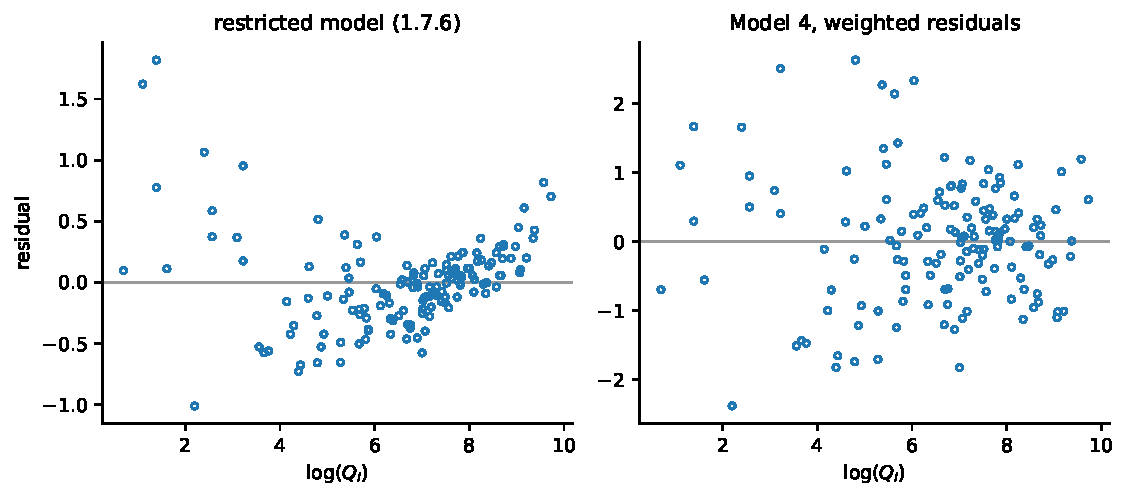
\includegraphics[width=0.95\textwidth]{figures/ch1_nerlove_residuals.pdf}
\end{center}
\begin{center}
\begin{minipage}{0.8\textwidth}\small
Figure S1.2: residuals against $\log(Q_i)$ for Nerlove's data.  Left: the restricted model \bk{(1.7.6)}.
Right: Model 4, estimated by weighted least squares.
\end{minipage}
\end{center}
\end{hee}

\problemset{1mc}{Problem Set for Chapter 1: Monte Carlo Exercise}

\begin{hmc}{1.1}{}
(a) \texttt{code/ch1.py} runs both simulations with $1{,}000{,}000$ replications, generating the regressor
by the book's matrix formula $\mathbf{x}=\mathbf{r}\,x_0+\mathbf{d}+\mathbf{A}\bs{\eta}$ with
$r_i=\phi^i$, $d_i=c(1-\phi^i)/(1-\phi)$ and $\mathbf{A}$ the lower-triangular Toeplitz matrix with
$A_{ij}=\phi^{i-j}$ for $i\ge j$.  The results are
\begin{center}
\begin{tabular}{lcc}
\toprule
 & simulation 1 ($\mathbf{x}$ fixed) & simulation 2 ($\mathbf{x}$ redrawn)\\
\midrule
mean of $b_1$ & $1.00049$ & ---\\
mean of $b_2$ & $0.49993$ & ---\\
$\Prob\{|t|>t_{0.025}(30)\}$ & $0.05003$ & $0.05011$\\
\bottomrule
\end{tabular}
\end{center}
With a million replications the standard error of a rejection frequency is
$\sqrt{0.05\cdot 0.95/10^6}=0.00022$, so both frequencies are within one standard error of $5\%$; the
average of $\mathbf{b}$ is within $0.0005$ of $\beta$.  The first simulation illustrates Proposition 1.1(a),
$\E(\mathbf{b}\given \mathbf{X})=\beta$, and the conditional statement of Proposition 1.3; the second
illustrates that the same $t$ distribution governs the \emph{unconditional} sampling behaviour, as argued in
Review Question 1.4.1 --- the conditional distribution does not depend on $\mathbf{x}$, so it is also the
marginal one.  Figure~S1.1 overlays the two simulated distributions of the $t$-ratio on the $t(30)$ density.

\begin{center}
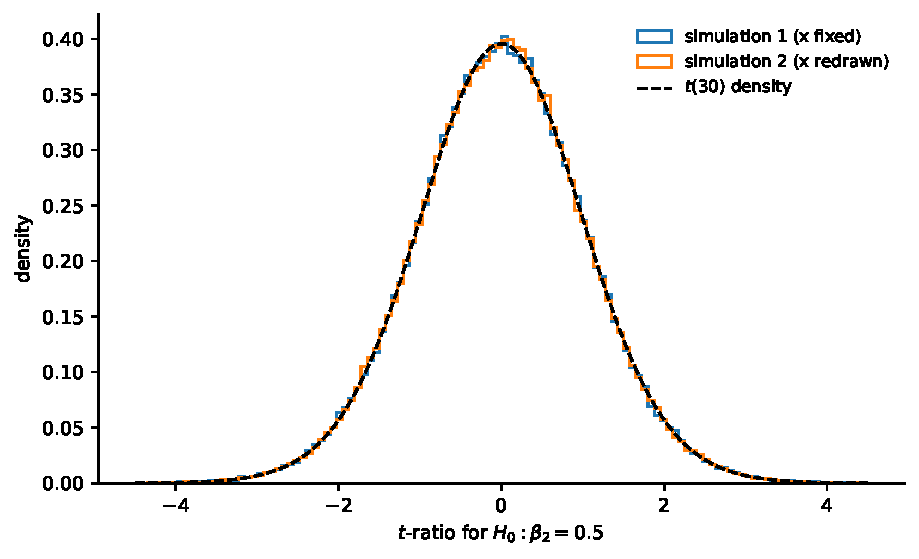
\includegraphics[width=0.78\textwidth]{figures/ch1_t_distribution.pdf}
\end{center}
\begin{center}
\begin{minipage}{0.8\textwidth}\small
Figure S1.1: the $t$-ratio for $H_0\colon\beta_2=0.5$ in the two simulations of the Monte Carlo exercise,
$10^6$ replications, against the $t(30)$ density.
\end{minipage}
\end{center}

(b) \emph{Strict exogeneity holds.}  The whole path $\mathbf{x}=(x_1,\dots,x_n)'$ is generated by
$(x_0,\bs{\eta})$, which is independent of $\bs{\varepsilon}$; hence
$\E(\varepsilon_i\given \mathbf{X})=\E(\varepsilon_i)=0$ for every $i$, which is Assumption 1.2 --- note that
this requires independence of $\varepsilon_i$ from \emph{all} the $x$'s, past and future, and that is exactly
how the design was built.  \emph{Conditional homoskedasticity holds} too:
$\E(\varepsilon_i^2\given \mathbf{X})=\E(\varepsilon_i^2)=1$ and
$\E(\varepsilon_i\varepsilon_j\given \mathbf{X})=0$ for $i\neq j$, so Assumption 1.4 is satisfied with
$\sigma^2=1$.  Together with normality (Assumption 1.5) and $\rank(\mathbf{X})=2$ almost surely, the design
satisfies Assumptions 1.1--1.5, which is why the simulated finite-sample results match the theory exactly.
\rmk{The sample is \emph{not} i.i.d.: $x_i$ is serially correlated, with
$\Corr(x_i,x_{i-1})=\phi=0.6$.  Serial correlation in the regressor is harmless here --- none of Assumptions
1.1--1.5 requires a random sample.  What would destroy strict exogeneity is feedback from the error to
later regressors, as in the autoregression $y_i=\beta_1+\beta_2y_{i-1}+\varepsilon_i$ of Chapter 2, where
only predeterminedness survives and the finite-sample results of this chapter no longer apply.}
\end{hmc}


%% ========================================================================
\solchapter{2}{Large-Sample Theory}

\begin{center}
\begin{minipage}{0.86\textwidth}
\small
Solutions to all the exercises of Chapter 2 of Fumio Hayashi, \emph{Econometrics} (Princeton University
Press, 2000): the 47 review questions of Sections 2.1--2.12, the twelve analytical exercises, the empirical
exercises on Mishkin's and Nerlove's data, and the two Monte Carlo exercises.  Assumptions, lemmas, propositions and
equations cited as \bk{Assumption 2.3}, \bk{Lemma 2.4(c)} or \bk{(2.3.1)} refer to the book.  The numerical
parts are computed by \texttt{code/ch2.py}.
\end{minipage}
\end{center}

\bigskip
\hrule
\bigskip

\solsection{2.1}{Review of Limit Theorems for Sequences of Random Variables}

\begin{hrq}{2.1.1}{}
Yes, and for deterministic sequences the converse holds too, so the two notions coincide.

Let $\{z_n\}$ be real numbers with $z_n\to\alpha$ and fix $\varepsilon>0$.  By the definition of a limit
there is $N$ such that $|z_n-\alpha|<\varepsilon$ for all $n>N$.  For such $n$ the event
$\{|z_n-\alpha|>\varepsilon\}$ is empty, so
\[
\Prob\{|z_n-\alpha|>\varepsilon\}=0\qquad (n>N),
\]
and a fortiori $\Prob\{|z_n-\alpha|>\varepsilon\}\to0$, which is $z_n\convp\alpha$.  Conversely, if a
deterministic sequence did not converge to $\alpha$, some $\varepsilon>0$ would have
$|z_n-\alpha|>\varepsilon$ infinitely often, and along that subsequence
$\Prob\{|z_n-\alpha|>\varepsilon\}=1$, so $z_n\not\convp\alpha$.

Convergence in probability is therefore a genuine weakening only for genuinely random sequences: it allows
$z_n$ to differ from $\alpha$ by a lot, as long as the probability of doing so vanishes.
\end{hrq}

\begin{hrq}{2.1.2}{}
Both definitions in the text are elementwise; both displayed conditions are about the squared Euclidean
distance.  Write $K$ for the dimension.

\emph{Mean square.}  The identity
$\E[(\mathbf{z}_n-\mathbf{z})'(\mathbf{z}_n-\mathbf{z})]=\sum_{k=1}^K\E[(z_{nk}-z_k)^2]$ expresses the
displayed quantity as a sum of $K$ nonnegative terms.  A finite sum of nonnegative sequences converges to
zero if and only if each summand does, so
$\E[(\mathbf{z}_n-\mathbf{z})'(\mathbf{z}_n-\mathbf{z})]\to0$ if and only if $z_{nk}\convms z_k$ for every
$k$.

\emph{Probability.}  Let $d_n\equiv(\mathbf{z}_n-\bs{\alpha})'(\mathbf{z}_n-\bs{\alpha})$.  If
$\Prob\{d_n>\varepsilon\}\to0$ for every $\varepsilon>0$, then for each $k$, since
$(z_{nk}-\alpha_k)^2\le d_n$,
\[
\Prob\{|z_{nk}-\alpha_k|>\varepsilon\}=\Prob\{(z_{nk}-\alpha_k)^2>\varepsilon^2\}
\le \Prob\{d_n>\varepsilon^2\}\to0,
\]
so $z_{nk}\convp\alpha_k$.  Conversely, if every element converges in probability, then by the union bound
\[
\Prob\{d_n>\varepsilon\}
\le\sum_{k=1}^K\Prob\Bigl\{(z_{nk}-\alpha_k)^2>\frac{\varepsilon}{K}\Bigr\}\to0,
\]
because $d_n>\varepsilon$ forces at least one of the $K$ squared deviations to exceed $\varepsilon/K$.  So
for vectors of fixed dimension, elementwise convergence and convergence of the distance are the same thing.
\end{hrq}

\begin{hrq}{2.1.3}{}
Decompose
\[
\mathbf{A}_n\mathbf{x}_n=(\mathbf{A}_n-\mathbf{A})\mathbf{x}_n+\mathbf{A}\mathbf{x}_n .
\]
For the first term, apply \bk{Lemma 2.4(b)} row by row: the $\ell$-th row of $\mathbf{A}_n-\mathbf{A}$
converges in probability to $\mathbf{0}$, and $\mathbf{x}_n\convd \mathbf{x}$, so the $\ell$-th element of
$(\mathbf{A}_n-\mathbf{A})\mathbf{x}_n$ converges in probability to zero.  By Review Question 2.1.2 the
whole vector then converges in probability to $\mathbf{0}$:
$(\mathbf{A}_n-\mathbf{A})\mathbf{x}_n\convp\mathbf{0}$.

For the second term, $\mathbf{x}\mapsto \mathbf{A}\mathbf{x}$ is a continuous function that does not depend
on $n$, so \bk{Lemma 2.3(b)} gives $\mathbf{A}\mathbf{x}_n\convd \mathbf{A}\mathbf{x}$.

Now \bk{Lemma 2.4(a)} applies to the sum of a sequence converging in distribution and one converging in
probability to a constant:
\[
\mathbf{A}_n\mathbf{x}_n=\mathbf{A}\mathbf{x}_n+(\mathbf{A}_n-\mathbf{A})\mathbf{x}_n
\convd \mathbf{A}\mathbf{x}+\mathbf{0}=\mathbf{A}\mathbf{x}.
\]
In particular, if $\mathbf{x}\sim \Norm(\mathbf{0},\Sigma)$ then
$\mathbf{A}_n\mathbf{x}_n\convd \Norm(\mathbf{0},\mathbf{A}\Sigma\mathbf{A}')$, which is the form in which
the lemma is used throughout the chapter (with $\mathbf{A}_n$ a matrix of sample moments and $\mathbf{x}_n$
a normalized sample average).
\end{hrq}

\begin{hrq}{2.1.4}{}
Yes.  Write
\[
\hat\theta_n-\theta=\frac{1}{\sqrt{n}}\cdot\sqrt{n}(\hat\theta_n-\theta),
\]
a product of a deterministic sequence $1/\sqrt{n}\to0$ (hence $\convp 0$ by Review Question 2.1.1) and a
sequence converging in distribution.  By \bk{Lemma 2.4(b)} the product converges in probability to zero, so
$\hat\theta_n-\theta\convp0$.

The intuition: asymptotic normality says the estimation error is of order $n^{-1/2}$, which is in
particular $o_p(1)$.  The converse fails --- consistency says nothing about the rate, and an estimator can
be consistent with a non-normal limit distribution or a slower rate (as in the unit-root asymptotics of
Chapter 9, where the rate is $n$ and the limit is not normal).
\end{hrq}

\begin{hrq}{2.1.5}{}
By Kolmogorov's LLN, $\bar{z}_n\convp\mu$, and by the Lindeberg--Levy CLT
$\sqrt{n}(\bar{z}_n-\mu)\convd \Norm(0,\sigma^2)$.  Apply \bk{Lemma 2.5} (the delta method) with
$\beta=\mu$, $x_n=\bar{z}_n$ and $a(\beta)=1/\beta$, which is continuously differentiable in a
neighbourhood of $\mu$ because $\mu\neq0$, with
\[
A(\beta)=\frac{\partial a(\beta)}{\partial\beta}=-\frac{1}{\beta^2},
\qquad A(\mu)=-\frac{1}{\mu^2}.
\]
The delta method gives
\[
\sqrt{n}\Bigl(\frac{1}{\bar{z}_n}-\frac{1}{\mu}\Bigr)
\convd \Norm\bigl(0,\;A(\mu)\sigma^2A(\mu)'\bigr)
=\Norm\Bigl(0,\frac{\sigma^2}{\mu^4}\Bigr).
\]
The requirement $\mu\neq0$ is essential: at $\mu=0$ the function $1/\beta$ is not differentiable (indeed
$1/\bar{z}_n$ does not even converge), and the asymptotic variance $\sigma^2/\mu^4$ blows up as $\mu$
approaches zero --- the finite-sample counterpart of which is the notorious instability of ratio estimators
with a small denominator.
\end{hrq}

\solsection{2.2}{Fundamental Concepts in Time-Series Analysis}

\begin{hrq}{2.2.1}{}
For a covariance-stationary process,
$\Gamma_j\equiv\Cov(\mathbf{z}_i,\mathbf{z}_{i-j})=\E[(\mathbf{z}_i-\bs{\mu})(\mathbf{z}_{i-j}-\bs{\mu})']$
does not depend on $i$.  Replacing $i$ by $i+j$ therefore leaves it unchanged, so
\[
\Gamma_{-j}=\Cov(\mathbf{z}_i,\mathbf{z}_{i+j})=\Cov(\mathbf{z}_{i+j},\mathbf{z}_i)'
=\Cov(\mathbf{z}_{i},\mathbf{z}_{i-j})'=\Gamma_j' ,
\]
where the second equality is the general fact $\Cov(\mathbf{x},\mathbf{y})=\Cov(\mathbf{y},\mathbf{x})'$
and the third uses covariance stationarity to shift the index by $-j$.  For a scalar process this says
$\gamma_{-j}=\gamma_j$: the autocovariance function is symmetric, so only $j\ge0$ need be tabulated.  For a
vector process the transpose matters --- $\Gamma_j$ is generally not symmetric, because the cross covariance
between variable $a$ today and variable $b$ $j$ periods ago differs from that between $b$ today and $a$ $j$
periods ago.
\end{hrq}

\begin{hrq}{2.2.2}{}
The future is forecast \emph{exactly}: $\E(z_i\given z_1)=T_i(z_1)$, where $T_i$ is the $i$-th Chebyshev
polynomial of the first kind, defined by $\cos(i\theta)=T_i(\cos\theta)$.  For example
\[
\E(z_2\given z_1)=2z_1^2-1,\qquad \E(z_3\given z_1)=4z_1^3-3z_1 .
\]
The reason is that $z_i$ is a deterministic function of $z_1$.  Knowing $z_1=\cos(w)$ leaves two
possibilities, $w$ and $2\pi-w$, and both give the same $z_i$, since
$\cos\bigl(i(2\pi-w)\bigr)=\cos(2\pi i-i w)=\cos(i w)$.  So $z_i$ is measurable with respect to $z_1$, and
conditioning on $z_1$ returns $z_i$ itself.

Consequently $\{z_i\}$ is \emph{not} a martingale difference sequence: an m.d.s.\ requires
$\E(z_i\given z_{i-1},\dots,z_1)=0$, whereas here the conditional expectation is a nonzero polynomial in
$z_1$.  The example shows how weak ``white noise'' is.  Zero serial correlation restricts only \emph{linear}
prediction; it leaves the process open to perfect \emph{nonlinear} prediction.  The process is also not
strictly stationary and not ergodic, which is why the ergodic stationary martingale difference CLT cannot be
applied to it.
\end{hrq}

\begin{hrq}{2.2.3}{}
Write $I_{i}\equiv(\mathbf{z}_{i},\dots,\mathbf{z}_1)$ for the information available at date $i$, so that
the martingale property reads $\E(x_{i}\given I_{i-1})=x_{i-1}$ and $x_{i-1}$ is a function of $I_{i-1}$
(it is an element of $\mathbf{z}_{i-1}$).

Induct on $j$.  For $j=0$ the claim is the martingale property itself.  Suppose
$\E(x_{i+j}\given I_{i-1})=x_{i-1}$.  Then, by the law of iterated expectations applied to the two nested
information sets $I_{i-1}\subset I_{i+j}$,
\[
\E(x_{i+j+1}\given I_{i-1})
=\E\bigl[\E(x_{i+j+1}\given I_{i+j})\given I_{i-1}\bigr]
=\E(x_{i+j}\given I_{i-1})=x_{i-1},
\]
using the martingale property in the inner expectation.  This completes the induction, so
$\E(x_{i+j}\given I_{i-1})=x_{i-1}$ for every $j\ge0$.  Subtracting two consecutive statements,
\[
\E(x_{i+j+1}-x_{i+j}\given I_{i-1})=x_{i-1}-x_{i-1}=0 .
\]
In words: given today's information, no change in a martingale is anticipated, at any horizon.  Under Hall's
hypothesis (\bk{Example 2.5}) this is the statement that no \emph{predictable} part of future consumption
growth should be forecastable from current information --- the restriction that the empirical literature
tests by regressing consumption growth on lagged variables.
\end{hrq}

\begin{hrq}{2.2.4}{}
Write $g_i\equiv x_i\varepsilon_i$.

\emph{i.i.d.: no.}  The $g_i$ are independent (see below) but not identically distributed:
$\Var(g_i)=x_i^2\sigma^2$ changes with $i$ because $x_i$ does.

\emph{Serially independent: yes.}  $g_i$ is a fixed (nonrandom) multiple of $\varepsilon_i$, and the
$\varepsilon_i$ are independent across $i$; multiplying independent random variables by constants preserves
independence.

\emph{m.d.s.: yes.}  $\E(g_i)=x_i\E(\varepsilon_i)=0$ and, by independence,
$\E(g_i\given g_{i-1},\dots,g_1)=x_i\E(\varepsilon_i\given \varepsilon_{i-1},\dots,\varepsilon_1)
=x_i\E(\varepsilon_i)=0$.

\emph{Stationary: no.}  Not even covariance stationary, since the variance $x_i^2\sigma^2$ depends on $i$;
a fortiori not strictly stationary.

The example matters for the theory of this chapter: the martingale difference CLT of Billingsley requires
\emph{ergodic stationary} m.d.s., and this process is an m.d.s.\ that fails stationarity.  Heteroskedastic
regression errors are exactly of this type, which is why Chapter 2 assumes ergodic stationarity of
$\{\mathbf{g}_i\}=\{\mathbf{x}_i\varepsilon_i\}$ rather than deriving it.
\end{hrq}

\begin{hrq}{2.2.5}{}
Let $z_i=g_1+\dots+g_i$ with $\{g_i\}$ independent white noise, $\E(g_i)=0$, $\Var(g_i)=\sigma^2>0$.  The
mean is constant ($\E(z_i)=0$), but by independence
\[
\Var(z_i)=\sum_{k=1}^i\Var(g_k)=i\,\sigma^2 ,
\]
which grows without bound and depends on $i$.  Covariance stationarity requires the variance to be the same
for all $i$, so a random walk is not covariance stationary, hence not stationary.  The autocovariances
inherit the same defect: $\Cov(z_i,z_{i-j})=(i-j)\sigma^2$ depends on $i$ as well as on $j$, and the
correlation $\Corr(z_i,z_{i-j})=\sqrt{(i-j)/i}$ tends to one for fixed $j$ --- a random walk is very far from
the asymptotic independence that ergodicity requires.  Chapter 9 develops the asymptotics for such
processes; the tools of this chapter do not apply to them.
\end{hrq}

\begin{hrq}{2.2.6}{}
Let $\{\mathbf{z}_i\}$ be a martingale and let $\mathbf{g}_i\equiv \mathbf{z}_i-\mathbf{z}_{i-1}$ be its
first differences, as in \bk{(2.2.7)}.  The two sequences carry the same information: knowing
$(\mathbf{z}_1,\dots,\mathbf{z}_{i-1})$ is the same as knowing $(\mathbf{g}_1,\dots,\mathbf{g}_{i-1})$,
since each can be computed from the other by differencing or cumulating.  Hence
\[
\E(\mathbf{g}_i\given \mathbf{g}_{i-1},\dots,\mathbf{g}_1)
=\E(\mathbf{z}_i-\mathbf{z}_{i-1}\given \mathbf{z}_{i-1},\dots,\mathbf{z}_1)
=\E(\mathbf{z}_i\given \mathbf{z}_{i-1},\dots,\mathbf{z}_1)-\mathbf{z}_{i-1}
=\mathbf{z}_{i-1}-\mathbf{z}_{i-1}=\mathbf{0},
\]
using \bk{(2.2.5)} and the fact that $\mathbf{z}_{i-1}$ is known given the conditioning variables.  Taking
unconditional expectations gives $\E(\mathbf{g}_i)=\mathbf{0}$, so $\{\mathbf{g}_i\}$ is an m.d.s.  With
\bk{(2.2.8)}, which cumulates an m.d.s.\ into a martingale, the two concepts are two views of the same
object: martingales are the running sums of martingale differences.
\end{hrq}

\begin{hrq}{2.2.7}{}
Condition on the past of $\{g_i\}$ and insert the finer information set generated by the $\varepsilon$'s,
which includes it, since $(g_{i-1},\dots,g_2)$ is a function of $(\varepsilon_{i-1},\dots,\varepsilon_1)$:
\[
\E(g_i\given g_{i-1},\dots,g_2)
=\E\bigl[\E(\varepsilon_i\varepsilon_{i-1}\given \varepsilon_{i-1},\dots,\varepsilon_1)
\given g_{i-1},\dots,g_2\bigr]
=\E\bigl[\varepsilon_{i-1}\E(\varepsilon_i)\given g_{i-1},\dots,g_2\bigr]=0,
\]
because $\varepsilon_i$ is independent of its own past with mean zero.  Hence $\{g_i\}$ is an m.d.s., and by
the proposition proved in the text it has no serial correlation.

It is not, however, independent white noise: $g_i$ and $g_{i-1}$ share the factor $\varepsilon_{i-1}$ and
are dependent, even though uncorrelated.  With $\varepsilon_i\sim \Norm(0,\sigma^2)$, for instance,
\[
\Cov(g_i^2,g_{i-1}^2)=\E(\varepsilon_i^2\varepsilon_{i-1}^4\varepsilon_{i-2}^2)
-\bigl[\E(\varepsilon_i^2\varepsilon_{i-1}^2)\bigr]^2
=\sigma^2\cdot3\sigma^4\cdot\sigma^2-\sigma^8=2\sigma^8>0 :
\]
squared values are positively correlated, which is precisely the volatility clustering that ARCH models of
\bk{(2.2.10)} are built to capture.
\end{hrq}

\begin{hrq}{2.2.8}{}
Write $I_k\equiv(y_k,\dots,y_1)$.  Both terms of $r_{i1}$ are conditional expectations of the same random
variable on nested information sets $I_{i-2}\subset I_{i-1}$.  Condition on the smaller one and use the law
of iterated expectations on the first term, while the second is already a function of $I_{i-2}$:
\[
\E(r_{i1}\given I_{i-2})
=\E\bigl[\E(y_i\given I_{i-1})\given I_{i-2}\bigr]-\E(y_i\given I_{i-2})
=\E(y_i\given I_{i-2})-\E(y_i\given I_{i-2})=0 .
\]
Now note that $r_{j1}$ for $j\le i-1$ is a function of $I_{j-1}\subset I_{i-2}$.  Conditioning the display
down to the past revisions therefore gives
\[
\E(r_{i1}\given r_{i-1,1},\dots,r_{21})
=\E\bigl[\E(r_{i1}\given I_{i-2})\given r_{i-1,1},\dots,r_{21}\bigr]=0,
\]
so $\{r_{i1}\}$ is a martingale difference sequence (with mean zero, by one more application of iterated
expectations).  Revisions to a forecast are unforecastable from information already used in making it ---
if they were not, the forecast would not have been optimal.
\rmk{The conditioning set has to be $I_{i-2}$, the information on which the \emph{second} term is based.
Conditional on $I_{i-1}$ the revision is not zero but equal to itself: $\E(r_{i1}\given I_{i-1})=r_{i1}$,
because both terms are then known.  The exercise's phrase ``m.d.s.\ with respect to $\{y_i\}$'' should be read
in this sense.}
\end{hrq}

\begin{hrq}{2.2.9}{}
Put $\mathbf{g}_i\equiv \mathbf{z}_i-\bs{\mu}$.  Then:

\emph{$\{\mathbf{g}_i\}$ is stationary and ergodic.}  It is i.i.d.\ (a fixed shift of an i.i.d.\ sequence),
hence strictly stationary; and an i.i.d.\ sequence is ergodic, since variables far apart in the sequence are
not merely asymptotically independent but exactly independent, so the defining factorization
$|\E[f(\mathbf{g}_i,\dots)g(\mathbf{g}_{i+n},\dots)]|=|\E[f]|\,|\E[g]|$ holds for every $n$.

\emph{$\{\mathbf{g}_i\}$ is an m.d.s.\ with $\E(\mathbf{g}_i\mathbf{g}_i')=\Sigma$.}  Independence gives
$\E(\mathbf{g}_i\given \mathbf{g}_{i-1},\dots,\mathbf{g}_1)=\E(\mathbf{g}_i)=\mathbf{0}$, and
$\E(\mathbf{g}_i\mathbf{g}_i')=\Var(\mathbf{z}_i)=\Sigma$, which is finite by hypothesis.

The martingale differences CLT applies to such a sequence and states that
$\sqrt{n}\,\bar{\mathbf{g}}_n\convd \Norm(\mathbf{0},\Sigma)$.  Since
$\bar{\mathbf{g}}_n=\bar{\mathbf{z}}_n-\bs{\mu}$, this is exactly the Lindeberg--Levy conclusion
\[
\sqrt{n}(\bar{\mathbf{z}}_n-\bs{\mu})\convd \Norm(\mathbf{0},\Sigma).
\]
So Lindeberg--Levy is the special case of the ergodic stationary m.d.s.\ CLT in which the martingale
differences happen to be i.i.d.  The gain from the more general theorem is exactly what large-sample
econometrics needs: it covers regression errors that are serially uncorrelated but conditionally
heteroskedastic and dependent, as in Review Question 2.2.7.
\end{hrq}

\solsection{2.3}{Large-Sample Distribution of the OLS Estimator}

\begin{hrq}{2.3.1}{}
First, the error has conditional mean zero:
\[
\E(\varepsilon_i\given \mathbf{x}_i)=\E(y_i\given \mathbf{x}_i)-\mathbf{x}_i'\beta=0,
\]
since $\mathbf{x}_i'\beta$ is a function of the conditioning variable.  Orthogonality then follows from the
law of total expectations:
\[
\E(\mathbf{g}_i)=\E(\mathbf{x}_i\cdot\varepsilon_i)
=\E\bigl[\E(\mathbf{x}_i\varepsilon_i\given \mathbf{x}_i)\bigr]
=\E\bigl[\mathbf{x}_i\,\E(\varepsilon_i\given \mathbf{x}_i)\bigr]=\mathbf{0},
\]
which is \bk{Assumption 2.3}.  The implication runs one way only: $\E(\varepsilon_i\given
\mathbf{x}_i)=0$ is strictly stronger than $\E(\mathbf{x}_i\varepsilon_i)=\mathbf{0}$, because the former
also forces $\E[h(\mathbf{x}_i)\varepsilon_i]=0$ for \emph{every} function $h$, not just for the
coordinates of $\mathbf{x}_i$.  Orthogonality is all the large-sample theory of this chapter needs, which is
why it is what \bk{Assumption 2.3} assumes.
\end{hrq}

\begin{hrq}{2.3.2}{}
(a) \emph{No.}  Ergodic stationarity (\bk{Assumption 2.2}) restricts the \emph{time-series} behaviour of
$\{y_i,\mathbf{x}_i\}$, not the size of its moments: a strictly stationary process can have infinite second
moments (an i.i.d.\ Cauchy sequence is stationary and ergodic).  \bk{Assumption 2.4} assumes the second
moments of the regressors are finite, and \bk{Assumption 2.5} assumes that
$\mathbf{S}=\E(\mathbf{g}_i\mathbf{g}_i')=\E(\varepsilon_i^2\mathbf{x}_i\mathbf{x}_i')$ exists, is finite
and is nonsingular; but a finite $\E(\varepsilon_i^2\mathbf{x}_i\mathbf{x}_i')$ does not by itself bound
$\E(\varepsilon_i^2)$, because the weights $x_{ik}x_{ij}$ could be small exactly where $\varepsilon_i^2$ is
large.  This is why \bk{Proposition 2.2} carries the proviso ``provided $\E(\varepsilon_i^2)$ exists and is
finite''.

(b) If $x_{i1}=1$, then the $(1,1)$ element of
$\E(\mathbf{g}_i\mathbf{g}_i')=\E(\varepsilon_i^2\mathbf{x}_i\mathbf{x}_i')$ is
\[
\E(\varepsilon_i^2x_{i1}^2)=\E(\varepsilon_i^2),
\]
and that element is finite because the whole matrix is, by \bk{Assumption 2.5}.  So with an intercept in the
regression --- the usual case --- the proviso is automatically satisfied.
\end{hrq}

\begin{hrq}{2.3.3}{}
Condition on $\mathbf{x}_i$ and use the law of total expectations:
\[
\mathbf{S}=\E(\varepsilon_i^2\mathbf{x}_i\mathbf{x}_i')
=\E\bigl[\E(\varepsilon_i^2\mathbf{x}_i\mathbf{x}_i'\given \mathbf{x}_i)\bigr]
=\E\bigl[\E(\varepsilon_i^2\given \mathbf{x}_i)\,\mathbf{x}_i\mathbf{x}_i'\bigr]
=\E\bigl[f(\mathbf{x}_i)\mathbf{x}_i\mathbf{x}_i'\bigr],
\]
the middle step because $\mathbf{x}_i\mathbf{x}_i'$ is a function of the conditioning variable and can be
pulled out of the inner expectation.  The expression makes the role of conditional heteroskedasticity
transparent: $\mathbf{S}$ is the matrix of second moments of the regressors \emph{weighted by the
conditional variance of the error}, so observations in regions of $\mathbf{x}$ where the error is noisy get
more weight.  Under conditional homoskedasticity $f(\mathbf{x}_i)\equiv\sigma^2$ and
$\mathbf{S}=\sigma^2\Sigma_{\mathbf{x}\mathbf{x}}$, which collapses the sandwich \bk{(2.3.4)} to
$\sigma^2\Sigma_{\mathbf{x}\mathbf{x}}^{-1}$ (Section 2.6).
\end{hrq}

\begin{hrq}{2.3.4}{}
Equation \bk{(2.3.11)} is the algebraic identity
\[
\frac1n\sum_{i=1}^n e_i^2=\frac1n\sum_{i=1}^n \varepsilon_i^2
-2(\mathbf{b}-\beta)'\bar{\mathbf{g}}+(\mathbf{b}-\beta)'\mathbf{S}_{\mathbf{x}\mathbf{x}}(\mathbf{b}-\beta),
\qquad \bar{\mathbf{g}}=\frac1n\sum_i\mathbf{x}_i\varepsilon_i .
\]
Under \bk{Assumptions 2.1--2.4} the proof of \bk{Proposition 2.1} has already established
\[
\mathbf{b}-\beta\convp\mathbf{0},\qquad
\bar{\mathbf{g}}\convp\E(\mathbf{g}_i)=\mathbf{0},\qquad
\mathbf{S}_{\mathbf{x}\mathbf{x}}\convp\Sigma_{\mathbf{x}\mathbf{x}}\ (\text{finite}).
\]
The maps $(\mathbf{u},\mathbf{v})\mapsto \mathbf{u}'\mathbf{v}$ and
$(\mathbf{u},\mathbf{A})\mapsto \mathbf{u}'\mathbf{A}\mathbf{u}$ are continuous and do not depend on $n$, so
\bk{Lemma 2.3(a)} lets the probability limits be taken inside:
\[
(\mathbf{b}-\beta)'\bar{\mathbf{g}}\convp \mathbf{0}'\mathbf{0}=0,
\qquad
(\mathbf{b}-\beta)'\mathbf{S}_{\mathbf{x}\mathbf{x}}(\mathbf{b}-\beta)
\convp \mathbf{0}'\Sigma_{\mathbf{x}\mathbf{x}}\mathbf{0}=0 .
\]
Therefore $\frac1n\sum_ie_i^2$ and $\frac1n\sum_i\varepsilon_i^2$ have the same probability limit, and the
latter is $\E(\varepsilon_i^2)$ by the ergodic theorem applied to the ergodic stationary process
$\{\varepsilon_i^2\}$ (finite by the proviso).  Hence $\frac1n\sum_ie_i^2\convp\E(\varepsilon_i^2)$, which
is \bk{Proposition 2.2}; and since $s^2=\frac{n}{n-K}\cdot\frac1n\sum_ie_i^2$ with $n/(n-K)\to1$, $s^2$ is
consistent as well.
\end{hrq}

\begin{hrq}{2.3.5}{}
Since $\hat\varepsilon_i=\varepsilon_i-\mathbf{x}_i'(\hat\beta-\beta)$, squaring and averaging gives the
same identity as before with $\hat\beta$ in place of $\mathbf{b}$:
\[
\frac1n\sum_i\hat\varepsilon_i^2=\frac1n\sum_i\varepsilon_i^2
-2(\hat\beta-\beta)'\Bigl(\frac1n\sum_i\mathbf{x}_i\varepsilon_i\Bigr)
+(\hat\beta-\beta)'\mathbf{S}_{\mathbf{x}\mathbf{x}}(\hat\beta-\beta).
\]
By ergodic stationarity and the assumed finiteness, the two sample averages converge:
$\frac1n\sum_i\mathbf{x}_i\varepsilon_i\convp\E(\mathbf{x}_i\varepsilon_i)$ and
$\mathbf{S}_{\mathbf{x}\mathbf{x}}\convp\E(\mathbf{x}_i\mathbf{x}_i')$, both finite.  They are multiplied
by $\hat\beta-\beta\convp\mathbf{0}$, so by \bk{Lemma 2.3(a)} the last two terms vanish in probability ---
\emph{whatever} the value of $\E(\mathbf{x}_i\varepsilon_i)$.  Hence
\[
\frac1n\sum_i\hat\varepsilon_i^2\convp\plim\frac1n\sum_i\varepsilon_i^2=\E(\varepsilon_i^2).
\]
The point of the generalization is that neither \bk{Assumption 2.3} (orthogonality) nor the use of OLS is
needed: consistency of the coefficient estimator is enough.  This is what makes the residual variance from,
say, the instrumental-variable estimators of Chapter 3 --- where the regressors are \emph{not} orthogonal to
the error --- a consistent estimator of $\E(\varepsilon_i^2)$.
\end{hrq}

\solsection{2.4}{Hypothesis Testing}

\begin{hrq}{2.4.1}{}
Yes.  By definition
$\mathit{SE}^*(b_k)=\sqrt{\widehat{\Avar(b_k)}/n}$, where $\widehat{\Avar(b_k)}$ is the $(k,k)$ element of
$\mathbf{S}_{\mathbf{x}\mathbf{x}}^{-1}\widehat{\mathbf{S}}\mathbf{S}_{\mathbf{x}\mathbf{x}}^{-1}$ and
converges in probability to the finite number $\Avar(b_k)$.  Since $1/n\to0$ and the square root is
continuous, \bk{Lemma 2.3(a)} gives
\[
\mathit{SE}^*(b_k)=\sqrt{\frac{\widehat{\Avar(b_k)}}{n}}\convp 0 .
\]
That is exactly as it should be: the standard error measures the sampling uncertainty about $b_k$, which
disappears as the estimator becomes consistent.  What does \emph{not} vanish is the $t$-ratio
$(b_k-\bar\beta_k)/\mathit{SE}^*(b_k)$ under the null, because numerator and denominator shrink at the same
rate $n^{-1/2}$; the ratio is asymptotically $\Norm(0,1)$ by \bk{(2.4.1)}.
\end{hrq}

\begin{hrq}{2.4.2}{}
Apply the delta method (\bk{Lemma 2.5}) to $a(\beta)=-\log(\beta)$, which for $\beta>0$ is continuously
differentiable with $A(\beta)=-1/\beta$.  From $\sqrt{n}(b-\beta)\convd \Norm(0,\Avar(b))$,
\[
\sqrt{n}(\hat\lambda-\lambda)\convd \Norm\Bigl(0,\;\frac{\Avar(b)}{\beta^2}\Bigr),
\qquad\text{so}\qquad
\Avar(\hat\lambda)=\frac{\Avar(b)}{\beta^{2}} .
\]
Replacing the unknowns by consistent estimates ($b$ for $\beta$, $\widehat{\Avar(b)}$ for $\Avar(b)$) and
dividing by $n$ to get the variance of $\hat\lambda$ itself,
\[
\mathit{SE}(\hat\lambda)=\sqrt{\frac{\widehat{\Avar(b)}/b^{2}}{n}}
=\frac{1}{b}\sqrt{\frac{\widehat{\Avar(b)}}{n}}=\frac{\mathit{SE}(b)}{b},
\]
as claimed (for $b>0$; in general the factor is $1/|b|$).  Standard errors of nonlinear functions of
estimates are always computed this way, and the same recipe with the Jacobian $\mathbf{A}(\hat\beta)$ covers
the vector case.
\end{hrq}

\begin{hrq}{2.4.3}{}
None of the three.  Write $\widehat{\mathbf{V}}\equiv\widehat{\Avar(\mathbf{b})}/n$ for the estimated
variance of $\mathbf{b}$, so that
$W=(\mathbf{R}\mathbf{b}-\mathbf{r})'\bigl[\mathbf{R}\widehat{\mathbf{V}}\mathbf{R}'\bigr]^{-1}
(\mathbf{R}\mathbf{b}-\mathbf{r})$.  Under the reparameterization,
\[
\wt{\mathbf{R}}\mathbf{b}-\wt{\mathbf{r}}=\mathbf{F}(\mathbf{R}\mathbf{b}-\mathbf{r}),
\qquad
\bigl[\wt{\mathbf{R}}\widehat{\mathbf{V}}\wt{\mathbf{R}}'\bigr]^{-1}
=\bigl[\mathbf{F}\mathbf{R}\widehat{\mathbf{V}}\mathbf{R}'\mathbf{F}'\bigr]^{-1}
=(\mathbf{F}')^{-1}\bigl[\mathbf{R}\widehat{\mathbf{V}}\mathbf{R}'\bigr]^{-1}\mathbf{F}^{-1},
\]
so that
\[
\wt{W}=(\mathbf{R}\mathbf{b}-\mathbf{r})'\mathbf{F}'(\mathbf{F}')^{-1}
\bigl[\mathbf{R}\widehat{\mathbf{V}}\mathbf{R}'\bigr]^{-1}\mathbf{F}^{-1}\mathbf{F}
(\mathbf{R}\mathbf{b}-\mathbf{r})=W .
\]
The statistic is numerically identical in every sample; hence its finite-sample distribution and its
asymptotic distribution --- $\chi^2(\#r)$ under the null --- are identical too.  The inverse in the middle
is what does the work: it undoes exactly the linear transformation applied to the restrictions.
\rmk{The invariance is a property of \emph{linear} reformulations.  It fails for nonlinear ones: the
restrictions $\beta_1\beta_2=1$ and $\beta_1-1/\beta_2=0$ describe the same null but give numerically
different Wald statistics, because the delta-method variance is evaluated at the estimate and depends on the
parameterization.  This non-invariance --- discussed in the text after the definition of $W$ --- is the main
practical drawback of the Wald principle relative to likelihood ratio tests.}
\end{hrq}

\solsection{2.5}{Estimating $\E(\varepsilon_i^2\mathbf{x}_i\mathbf{x}_i')$ Consistently}

\begin{hrq}{2.5.1}{}
No.  Expanding $e_i^2=(y_i-\mathbf{x}_i'\mathbf{b})^2$ inside \bk{(2.5.1)},
\[
\widehat{\mathbf{S}}=\frac1n\sum_i e_i^2\mathbf{x}_i\mathbf{x}_i'
=\underbrace{\frac1n\sum_i y_i^2\,\mathbf{x}_i\mathbf{x}_i'}_{\text{2nd moments of }y^2}
-\;2\,\frac1n\sum_i y_i\,(\mathbf{x}_i'\mathbf{b})\,\mathbf{x}_i\mathbf{x}_i'
+\;\frac1n\sum_i(\mathbf{x}_i'\mathbf{b})^2\,\mathbf{x}_i\mathbf{x}_i' .
\]
These involve sample averages of $y_i^2x_{ik}x_{i\ell}$, of $y_ix_{ij}x_{ik}x_{i\ell}$ and of
$x_{ih}x_{ij}x_{ik}x_{i\ell}$: third- and fourth-order cross moments of the data, which cannot be recovered
from the second-order moments $\mathbf{S}_{\mathbf{x}\mathbf{x}}$, $\mathbf{s}_{\mathbf{x}y}$,
$\mathbf{y}'\mathbf{y}/n$ and $\bar y$.

What remains true is that the robust standard errors can still be computed in \emph{one pass} over the
data: accumulate the $K^2(K+1)/2$-odd fourth-order sums above (or, more simply, compute $\mathbf{b}$ first
and then accumulate $e_i^2\mathbf{x}_i\mathbf{x}_i'$ in a second pass).  What is lost is the tidy fact that
one fixed, small set of second moments is a sufficient summary of the data for every statistic --- robust
inference needs genuinely more information about the sample, which is another way of saying that it uses
the empirical distribution of the residuals rather than a single variance parameter.
\end{hrq}

\begin{hrq}{2.5.2}{}
The two are the same sandwich, $(\mathbf{X}'\mathbf{X})^{-1}(\text{middle})(\mathbf{X}'\mathbf{X})^{-1}$,
with three differences.

\emph{What the middle matrix is.}  In Chapter 1 it is $\mathbf{X}'(\sigma^2\mathbf{V})\mathbf{X}$, built
from the \emph{true} conditional variance matrix
$\sigma^2\mathbf{V}=\E(\bs{\varepsilon}\bs{\varepsilon}'\given \mathbf{X})$, which is unknown; the formula
is therefore a theoretical object, not an estimator, unless $\mathbf{V}$ is known.  In \bk{(2.5.4$'$)} it is
$\mathbf{X}'\mathbf{B}\mathbf{X}$ with $\mathbf{B}=\diag(e_1^2,\dots,e_n^2)$, which is computable from the
data.  Note that $\mathbf{B}$ is not a good estimate of $\sigma^2\mathbf{V}$ element by element --- one
residual cannot estimate one variance --- and does not need to be: only the $K\times K$ average
$\mathbf{X}'\mathbf{B}\mathbf{X}/n$ has to converge, and it does, to $\mathbf{S}$.

\emph{Diagonality.}  $\mathbf{V}$ is an arbitrary positive definite matrix, so the Chapter 1 formula allows
serial correlation as well as heteroskedasticity.  $\mathbf{B}$ is diagonal: White's formula is valid only
because \bk{Assumption 2.5} makes $\{\mathbf{g}_i\}$ a martingale difference sequence, so that the
autocovariances of $\mathbf{g}_i$ vanish.  When they do not, $\mathbf{S}$ must be replaced by a long-run
variance matrix (Chapter 6).

\emph{What is being measured.}  $\Var(\mathbf{b}\given \mathbf{X})$ is the exact variance of $\mathbf{b}$
conditional on $\mathbf{X}$, and it requires strict exogeneity for unbiasedness to make sense;
$\widehat{\Avar(\mathbf{b})}$ estimates the variance of the asymptotic distribution of $\sqrt{n}(\mathbf{b}
-\beta)$ --- hence the factor $n$ --- and needs only predeterminedness.  Dividing \bk{(2.5.4$'$)} by $n$
gives $(\mathbf{X}'\mathbf{X})^{-1}(\mathbf{X}'\mathbf{B}\mathbf{X})(\mathbf{X}'\mathbf{X})^{-1}$, which is
the direct analogue of the Chapter 1 expression with $\sigma^2\mathbf{V}$ replaced by $\mathbf{B}$.
\end{hrq}

\solsection{2.6}{Implications of Conditional Homoskedasticity}

\begin{hrq}{2.6.1}{}
No to both.  The estimator \bk{(2.6.2)} is $s^2\mathbf{S}_{\mathbf{x}\mathbf{x}}^{-1}$, and since
$s^2\convp\E(\varepsilon_i^2)\equiv\sigma^2$ and
$\mathbf{S}_{\mathbf{x}\mathbf{x}}\convp\Sigma_{\mathbf{x}\mathbf{x}}$,
\[
s^2\mathbf{S}_{\mathbf{x}\mathbf{x}}^{-1}\convp \sigma^2\Sigma_{\mathbf{x}\mathbf{x}}^{-1},
\qquad\text{whereas}\qquad
\Avar(\mathbf{b})=\Sigma_{\mathbf{x}\mathbf{x}}^{-1}\mathbf{S}\Sigma_{\mathbf{x}\mathbf{x}}^{-1}.
\]
These agree if and only if $\mathbf{S}=\E(\varepsilon_i^2\mathbf{x}_i\mathbf{x}_i')
=\sigma^2\Sigma_{\mathbf{x}\mathbf{x}}$, that is, if and only if
$\E\bigl[\bigl(\E(\varepsilon_i^2\given \mathbf{x}_i)-\sigma^2\bigr)\mathbf{x}_i\mathbf{x}_i'\bigr]
=\mathbf{0}$ (Review Question 2.3.3).  Conditional homoskedasticity makes the bracket zero; without it the
two matrices generally differ, in either direction --- the conventional standard errors can be too small or
too large.

The $t$-ratio inherits the failure.  Under $H_0\colon\beta_k=\bar\beta_k$,
\[
t_k=\frac{\sqrt{n}(b_k-\bar\beta_k)}{\sqrt{s^2[\mathbf{S}_{\mathbf{x}\mathbf{x}}^{-1}]_{kk}}}
\convd \Norm\Bigl(0,\;\frac{[\Avar(\mathbf{b})]_{kk}}
{\sigma^2[\Sigma_{\mathbf{x}\mathbf{x}}^{-1}]_{kk}}\Bigr),
\]
by \bk{Lemma 2.4(c)}: the numerator is asymptotically $\Norm(0,[\Avar(\mathbf{b})]_{kk})$ and the
denominator converges to the wrong constant.  The limit is standard normal only if the ratio in the
variance is one.  So without conditional homoskedasticity the conventional $t$ must be replaced by the
robust $t$ of \bk{(2.4.1)}; the critical values of $\Norm(0,1)$ applied to the conventional $t$ give a test
whose true asymptotic size is not the nominal one.
\end{hrq}

\begin{hrq}{2.6.2}{}
\emph{Consistency.}  Yes.  \bk{(2.3.5)},
$\mathbf{S}_{\mathbf{x}\mathbf{x}}^{-1}\widehat{\mathbf{S}}\mathbf{S}_{\mathbf{x}\mathbf{x}}^{-1}$, is
consistent for $\Sigma_{\mathbf{x}\mathbf{x}}^{-1}\mathbf{S}\Sigma_{\mathbf{x}\mathbf{x}}^{-1}$ whether or
not \bk{Assumption 2.7} holds (given \bk{Assumption 2.6}); when it does hold, that limit \emph{is}
$\sigma^2\Sigma_{\mathbf{x}\mathbf{x}}^{-1}$.  Robust standard errors are therefore valid under conditional
homoskedasticity as well --- they are never wrong asymptotically, only unnecessary.

\emph{Advantage of \bk{(2.6.2)}: fewer parameters.}  To form \bk{(2.6.2)} one estimates
$\Sigma_{\mathbf{x}\mathbf{x}}$ and the single scalar $\sigma^2$: $K(K+1)/2+1$ population parameters.  To
form \bk{(2.3.5)} one estimates $\Sigma_{\mathbf{x}\mathbf{x}}$ \emph{and} the whole matrix
$\mathbf{S}=\E(\varepsilon_i^2\mathbf{x}_i\mathbf{x}_i')$: $K(K+1)$ parameters, and the elements of
$\widehat{\mathbf{S}}$ are averages of fourth-order products, which are noisy.  With $K=5$, that is $16$
parameters against $30$.  Since the finite-sample behaviour of an estimator deteriorates with the number of
parameters being estimated, the conventional standard errors are the more reliable ones \emph{when the
homoskedasticity assumption is true} --- this is the trade-off behind the Monte Carlo evidence cited in
Section 2.5 that robust $t$-ratios over-reject in small samples.
\end{hrq}

\begin{hrq}{2.6.3}{}
From the tables (or \texttt{code/ch2.py}),
\[
F_{0.05}(10,\infty)=1.8307,\qquad \chi^2_{0.05}(10)=18.307=10\times1.8307 .
\]
The relation is $\chi^2_{\alpha}(m)=m\cdot F_\alpha(m,\infty)$, which follows from the construction of the
$F$ distribution: $F(m_1,m_2)$ is the ratio of two independent chi-squares divided by their degrees of
freedom, and as $m_2\to\infty$ the denominator $\chi^2(m_2)/m_2\convp1$, so
$F(m,\infty)\eqd\chi^2(m)/m$.  That is exactly why \bk{Proposition 2.5(c)} states that $\#r\cdot F$, not
$F$, is asymptotically $\chi^2(\#r)$: multiplying by the number of restrictions converts the
$F$-scale into the $\chi^2$-scale.  Since $F(\#r,n-K)\to F(\#r,\infty)$ as $n\to\infty$, using the
$F(\#r,n-K)$ table on $F$ and the $\chi^2(\#r)$ table on $\#r\cdot F$ are asymptotically the same test, the
former being slightly more conservative in finite samples.
\end{hrq}

\begin{hrq}{2.6.4}{}
No.  By Analytical Exercise 1.5 the statistic equals $\#r\cdot F$, which in the notation of this chapter is
\[
\#r\cdot F=\sqrt{n}(\mathbf{R}\mathbf{b}-\mathbf{r})'
\bigl[s^2\mathbf{R}\mathbf{S}_{\mathbf{x}\mathbf{x}}^{-1}\mathbf{R}'\bigr]^{-1}
\sqrt{n}(\mathbf{R}\mathbf{b}-\mathbf{r}).
\]
Under the null $\sqrt{n}(\mathbf{R}\mathbf{b}-\mathbf{r})\convd \mathbf{x}\sim
\Norm(\mathbf{0},\Omega)$ with $\Omega=\mathbf{R}\Avar(\mathbf{b})\mathbf{R}'$, while the middle matrix
converges to $\mathbf{A}=\sigma^2\mathbf{R}\Sigma_{\mathbf{x}\mathbf{x}}^{-1}\mathbf{R}'$.  Hence
\[
\#r\cdot F\convd \mathbf{x}'\mathbf{A}^{-1}\mathbf{x}
\eqd \sum_{j=1}^{\#r}\lambda_j\,w_j,\qquad w_j\ \text{i.i.d.}\ \chi^2(1),
\]
where $\lambda_1,\dots,\lambda_{\#r}$ are the eigenvalues of $\mathbf{A}^{-1}\Omega$.  This is $\chi^2(\#r)$
if and only if all the $\lambda_j$ equal one, that is, $\Omega=\mathbf{A}$ --- precisely what conditional
homoskedasticity delivers.  Otherwise the statistic has a weighted sum of chi-squares as its limit, with
both mean and critical values different from those of $\chi^2(\#r)$.  The remedy is the robust Wald
statistic \bk{(2.4.2)}, which replaces $\mathbf{A}$ by a consistent estimate of $\Omega$.
\end{hrq}

\begin{hrq}{2.6.5}{}
By Analytical Exercise 1.6(b), the $F$-statistic for the null equals
\[
F=\frac{R^2/(K-1)}{(1-R^2)/(n-K)}
\quad\Longleftrightarrow\quad
(K-1)F=\frac{n-K}{n}\cdot\frac{nR^2}{1-R^2}.
\]
\bk{Proposition 2.5(c)} gives $(K-1)F\convd\chi^2(K-1)$.  Under the null, $R^2\convp0$: the numerator of
$R^2$ is $\frac1n\sum_i(\hat y_i-\bar y)^2=(\mathbf{b}-\hat\beta)'\mathbf{S}_{\mathbf{x}\mathbf{x}}
(\mathbf{b}-\hat\beta)\convp0$ because $\mathbf{b}$ converges to the true coefficient vector whose slopes
are zero, while the denominator converges to $\Var(y_i)>0$.  Solving the display for $nR^2$,
\[
nR^2=(K-1)F\cdot(1-R^2)\cdot\frac{n}{n-K},
\]
a product of a sequence converging in distribution to $\chi^2(K-1)$ and a sequence converging in
probability to $1\cdot 1=1$.  By \bk{Lemma 2.4(c)} (or (2.1.8)), $nR^2\convd\chi^2(K-1)$.

\emph{Without conditional homoskedasticity: no.}  The argument rests entirely on
\bk{Proposition 2.5(c)}, which assumes \bk{Assumption 2.7}; by Review Question 2.6.4 the statistic then has
a weighted-chi-square limit.  This matters in practice because $nR^2$ statistics are ubiquitous as
Lagrange-multiplier tests --- including White's test of Section 2.7 and the Breusch--Godfrey test of
Section 2.10, both of which need their own homoskedasticity-type condition for the $\chi^2$ approximation.
\end{hrq}

\solsection{2.7}{Testing Conditional Homoskedasticity}

\begin{hrq}{2.7.1}{}
The products of the four entries with one another are
\[
\begin{array}{c|cccc}
 & 1 & q & q^2 & p\\\hline
1 & 1 & q & q^2 & p\\
q &   & q^2 & q^3 & qp\\
q^2 & & & q^4 & q^2p\\
p & & & & p^2
\end{array}
\]
Discarding the constant $1$ and counting each distinct monomial once ($q^2$ appears twice, as $1\cdot q^2$
and as $q\cdot q$), the distinct nonconstant elements are
\[
q,\quad q^2,\quad q^3,\quad q^4,\quad p,\quad qp,\quad q^2p,\quad p^2,
\]
that is, $8$ of them, so $\bs{\psi}_i$ is $8$-dimensional and White's auxiliary regression of $e_i^2$ on a
constant and $\bs{\psi}_i$ has $9$ coefficients; the test statistic is $nR^2\convd\chi^2(8)$.

The count also shows why White's test loses power in larger models: with $K$ regressors the number of
distinct products is at most $K(K+1)/2-1$ nonconstant terms, which grows quadratically, so the degrees of
freedom (and with them the critical value) grow fast while the alternative may concentrate on one or two of
the terms.  Dropping from $\bs{\psi}_i$ those variables that theory says cannot affect the conditional
variance raises power --- at the cost of no power at all against the alternatives so excluded.
\end{hrq}

\solsection{2.8}{Estimation with Parameterized Conditional Heteroskedasticity}

\begin{hrq}{2.8.1}{}
Since $\mathbf{z}_i=\mathbf{z}(\mathbf{x}_i)$ is known once $\mathbf{x}_i$ is,
\[
\E(\mathbf{z}_i\eta_i)
=\E\bigl[\E(\mathbf{z}_i\eta_i\given \mathbf{x}_i)\bigr]
=\E\bigl[\mathbf{z}_i\,\E(\eta_i\given \mathbf{x}_i)\bigr]
=\E[\mathbf{z}_i\cdot 0]=\mathbf{0}.
\]
This is the step that makes the auxiliary regression \bk{(2.8.8)} of $\varepsilon_i^2$ on $\mathbf{z}_i$
legitimate: the regressors $\mathbf{z}_i$, being functions of $\mathbf{x}_i$, are orthogonal to its error
$\eta_i\equiv\varepsilon_i^2-\E(\varepsilon_i^2\given \mathbf{x}_i)$, so \bk{Proposition 2.1} applies and
OLS estimates $\bs{\alpha}$ consistently.  The same argument, applied to
$\wt{\mathbf{x}}_i=\mathbf{x}_i/\sqrt{\mathbf{z}_i'\bs{\alpha}}$ and
$\wt{\varepsilon}_i=\varepsilon_i/\sqrt{\mathbf{z}_i'\bs{\alpha}}$, verifies \bk{Assumption 2.3} for the
weighted equation.
\end{hrq}

\begin{hrq}{2.8.2}{}
Generally \emph{no}.  The error of \bk{(2.8.8)} is
$\eta_i=\varepsilon_i^2-\E(\varepsilon_i^2\given \mathbf{x}_i)$, whose conditional second moment is
\[
\E(\eta_i^2\given \mathbf{x}_i)=\Var(\varepsilon_i^2\given \mathbf{x}_i)
=\E(\varepsilon_i^4\given \mathbf{x}_i)-\bigl[\E(\varepsilon_i^2\given \mathbf{x}_i)\bigr]^2 ,
\]
a function of $\mathbf{x}_i$ in all but contrived cases.  If, for instance, $\varepsilon_i$ is
conditionally normal, $\E(\eta_i^2\given \mathbf{x}_i)=2(\mathbf{z}_i'\bs{\alpha})^2$, which varies with
$\mathbf{x}_i$ whenever the model is heteroskedastic at all --- the very situation the auxiliary regression
is run in.

\emph{Does it matter for the WLS estimator?  No.}  What the WLS procedure needs from Step 2 is
consistency of $\hat{\bs{\alpha}}$, and \bk{Proposition 2.1(a)} delivers that without any homoskedasticity
assumption.  As stated in the text, $\sqrt{n}(\hat\beta(\widehat{\mathbf{V}})-\beta)$ and
$\sqrt{n}(\hat\beta(\mathbf{V})-\beta)$ are asymptotically equivalent, so the sampling error in
$\hat{\bs{\alpha}}$ --- and hence its variance --- washes out of the asymptotic distribution of the WLS
estimator entirely.

It does matter if one wants to do \emph{inference about $\bs{\alpha}$ itself} (for example to test whether
some element of $\mathbf{z}_i$ belongs in the skedastic function): there the conventional standard errors
from Step 2 are invalid and robust ones should be used.
\end{hrq}

\solsection{2.9}{Least Squares Projection}

\begin{hrq}{2.9.1}{}
By construction $\E(\eta\given \mathbf{x})=\E(y\given \mathbf{x})-\E(y\given \mathbf{x})=0$.  Hence, for any
$\phi$ such that the expectation exists,
\[
\E[\eta\,\phi(\mathbf{x})]=\E\bigl[\E(\eta\,\phi(\mathbf{x})\given \mathbf{x})\bigr]
=\E\bigl[\phi(\mathbf{x})\E(\eta\given \mathbf{x})\bigr]=0 .
\]
Applying this with $\phi(\mathbf{x})=\E(y\given \mathbf{x})-f(\mathbf{x})$ kills the cross term in the mean
squared error decomposition \bk{(2.9.3)}:
\[
\E\bigl[(y-f(\mathbf{x}))^2\bigr]
=\underbrace{\E[\eta^2]}_{\text{unavoidable}}
+\E\bigl[\bigl(\E(y\given \mathbf{x})-f(\mathbf{x})\bigr)^2\bigr],
\]
so that the conditional expectation is the minimum mean squared error forecast: any other $f$ adds a
nonnegative term.  The identity is also the source of the orthogonality that defines the least squares
projection, with $\phi$ restricted to linear functions.
\end{hrq}

\begin{hrq}{2.9.2}{}
\emph{Both projections are zero.}  Write $\mathbf{w}\equiv(\varepsilon_{i-1},\dots,\varepsilon_{i-m})'$.
The projection coefficients on the lags alone are
\[
\bigl[\E(\mathbf{w}\mathbf{w}')\bigr]^{-1}\E(\mathbf{w}\varepsilon_i),
\]
and every element of $\E(\mathbf{w}\varepsilon_i)$ is an autocovariance $\gamma_j$ with $j\ge1$, which is
zero for white noise.
With a constant included, \bk{(2.9.7)} gives
$\bs{\gamma}=\Var(\mathbf{w})^{-1}\Cov(\mathbf{w},\varepsilon_i)=\mathbf{0}$ and
$\mu=\E(\varepsilon_i)-\bs{\gamma}'\E(\mathbf{w})=0$.  So the best \emph{linear} forecast of white noise
from its own past is the unconditional mean, zero.

\emph{The conditional expectation need not be zero.}  Example 2.4 makes the point: for
$\varepsilon_i=\cos(i\,w)$ the process is white noise, yet by Review Question 2.2.2
$\E(\varepsilon_i\given \varepsilon_{i-1})$ is a nonzero polynomial in $\varepsilon_{i-1}$ --- the past
predicts the present perfectly, nonlinearly.  Zero autocorrelation restricts only the linear projection; it
is the martingale difference property, not white noise, that sets the conditional expectation to zero.
\end{hrq}

\begin{hrq}{2.9.3}{}
Use the formula \bk{(2.9.7)} for the projection with a constant and compute its ingredients from the
assumed conditional mean.  Since $\Cov(\wt{\mathbf{x}},y)=\Cov\bigl(\wt{\mathbf{x}},
\E(y\given \wt{\mathbf{x}})\bigr)$ by the law of total covariance (the part of $y$ orthogonal to every
function of $\wt{\mathbf{x}}$ contributes nothing),
\[
\Cov(\wt{\mathbf{x}},y)=\Cov(\wt{\mathbf{x}},\mu+\bs{\gamma}'\wt{\mathbf{x}})
=\Var(\wt{\mathbf{x}})\bs{\gamma}
\ \Longrightarrow\
\bs{\gamma}^{\,*}=\Var(\wt{\mathbf{x}})^{-1}\Cov(\wt{\mathbf{x}},y)=\bs{\gamma},
\]
and then
$\mu^*=\E(y)-\bs{\gamma}'\E(\wt{\mathbf{x}})=\bigl[\mu+\bs{\gamma}'\E(\wt{\mathbf{x}})\bigr]
-\bs{\gamma}'\E(\wt{\mathbf{x}})=\mu$.  So the projection coefficients coincide with the coefficients of
the conditional expectation.

The same conclusion follows in one line from Review Question 2.9.1: the conditional expectation minimizes
the mean squared error among \emph{all} functions; if it happens to be linear, it also minimizes among
linear functions, which is the definition of the projection.  This is the situation in which OLS estimates
a conditional expectation rather than merely a linear approximation to it --- for instance under joint
normality (Review Question 1.1.4) or when the regressors are a saturated set of dummies.
\end{hrq}

\begin{hrq}{2.9.4}{}
(a) Write $\mathbf{w}_i\equiv(\mathbf{x}_i',\mathbf{z}_i')'$.  Because
$\E(\mathbf{z}_i\mathbf{x}_i')=\mathbf{0}$, the second moment matrix is block diagonal, so
\[
\wh{\E}^*(\varepsilon_i\given \mathbf{x}_i,\mathbf{z}_i)
=\Bigl[\E(\mathbf{w}_i\mathbf{w}_i')^{-1}\E(\mathbf{w}_i\varepsilon_i)\Bigr]'\mathbf{w}_i
=\mathbf{0}'\mathbf{x}_i+\bigl[\E(\mathbf{z}_i\mathbf{z}_i')^{-1}\E(\mathbf{z}_i\varepsilon_i)\bigr]'
\mathbf{z}_i .
\]
Projections are linear, so projecting $y_i=\mathbf{x}_i'\beta+\mathbf{z}_i'\delta+\varepsilon_i$ gives
\[
\wh{\E}^*(y_i\given \mathbf{x}_i,\mathbf{z}_i)
=\mathbf{x}_i'\beta+\mathbf{z}_i'\bigl[\delta+\E(\mathbf{z}_i\mathbf{z}_i')^{-1}
\E(\mathbf{z}_i\varepsilon_i)\bigr].
\]
The coefficient of $\mathbf{x}_i$ is $\beta$ --- the endogeneity of $\mathbf{z}_i$ contaminates only the
coefficient of $\mathbf{z}_i$, because $\mathbf{z}_i$ is uncorrelated with $\mathbf{x}_i$.

(b) Treating $\mathbf{z}_i'\delta+\varepsilon_i$ as the error,
\[
\E(\mathbf{x}_i\mathbf{x}_i')^{-1}\E(\mathbf{x}_iy_i)
=\beta+\E(\mathbf{x}_i\mathbf{x}_i')^{-1}\bigl[\E(\mathbf{x}_i\mathbf{z}_i')\delta
+\E(\mathbf{x}_i\varepsilon_i)\bigr]=\beta,
\]
again $\beta$, since both terms in the bracket vanish.  So OLS estimates $\beta$ consistently with or
without $\mathbf{z}_i$ in the regression.

(c) Use the long projection, on $(\mathbf{x}_i,\mathbf{z}_i)$.  Both are consistent, so the choice is about
precision, and the projection error is smaller in the long regression: adding regressors cannot increase
the mean squared projection error, and it strictly decreases it unless $\mathbf{z}_i$ has no explanatory
power at all.  Under conditional homoskedasticity the asymptotic variance of the $\beta$-block is
$\sigma_v^2\,\E(\mathbf{x}_i\mathbf{x}_i')^{-1}$ in the long regression and
$\sigma_u^2\,\E(\mathbf{x}_i\mathbf{x}_i')^{-1}$ in the short one (the block diagonality of the second
moment matrix leaves the $\mathbf{x}$ block untouched), with $\sigma_v^2\le\sigma_u^2$: including
$\mathbf{z}_i$ sharpens the estimate of $\beta$ even though the coefficient of $\mathbf{z}_i$ itself is
biased for $\delta$.
\end{hrq}

\solsection{2.10}{Testing for Serial Correlation}

\begin{hrq}{2.10.1}{}
Expand the product in \bk{(2.10.1)}:
\[
\hat\gamma_j=\frac1n\sum_{t=j+1}^{n}(z_t-\bar z_n)(z_{t-j}-\bar z_n)
=\frac1n\sum_{t=j+1}^{n}z_tz_{t-j}
-\bar z_n\frac1n\sum_{t=j+1}^{n}z_{t-j}
-\bar z_n\frac1n\sum_{t=j+1}^{n}z_t
+\frac{n-j}{n}(\bar z_n)^2 .
\]
Fix $j$ and let $n\to\infty$.  The process $\{z_tz_{t-j}\}$ is a measurable function of finitely many
coordinates of an ergodic stationary process, hence itself ergodic stationary, so the ergodic theorem gives
$\frac1n\sum_{t=j+1}^nz_tz_{t-j}\convp\E(z_tz_{t-j})$ (the $j$ missing terms change the average by
$O_p(j/n)$).  The same theorem gives $\bar z_n\convp\E(z_t)\equiv\mu_z$ and, again up to $j/n$,
$\frac1n\sum_{t=j+1}^nz_{t-j}\convp\mu_z$ and $\frac1n\sum_{t=j+1}^nz_t\convp\mu_z$; and
$(n-j)/n\to1$.  By \bk{Lemma 2.3(a)},
\[
\hat\gamma_j\convp \E(z_tz_{t-j})-\mu_z^2-\mu_z^2+\mu_z^2
=\E(z_tz_{t-j})-\E(z_t)\E(z_{t-j})=\gamma_j .
\]
Consistency of $\hat\rho_j=\hat\gamma_j/\hat\gamma_0$ then follows from \bk{Lemma 2.3(a)} applied to the
ratio, since $\gamma_0>0$.  Note that dividing by $n$ rather than $n-j$ is immaterial asymptotically, as
$(n-j)/n\to1$; it matters in moderate samples, which is why the text insists on saying which convention is
in use.
\end{hrq}

\begin{hrq}{2.10.2}{}
From \bk{(2.10.4)} and \bk{(2.10.5)}, with $\mathbf{x}_n\equiv\bigl((\sqrt{n}\hat\rho_1)^2,\dots,
(\sqrt{n}\hat\rho_p)^2\bigr)'$,
\[
Q_{\mathrm{LB}}-Q_{\mathrm{BP}}
=\sum_{j=1}^p\Bigl(\frac{n+2}{n-j}-1\Bigr)(\sqrt{n}\hat\rho_j)^2
=\mathbf{a}_n'\mathbf{x}_n,
\qquad
\mathbf{a}_n=\Bigl(\frac{j+2}{n-j}\Bigr)_{j=1,\dots,p}.
\]
For fixed $p$, $\mathbf{a}_n\to\mathbf{0}$ as $n\to\infty$, hence $\mathbf{a}_n\convp\mathbf{0}$ by Review
Question 2.1.1.  By \bk{Proposition 2.9} and the continuous mapping theorem,
$\mathbf{x}_n$ converges in distribution (to a vector of independent $\chi^2(1)$ variables).  \bk{Lemma
2.4(b)} then gives $\mathbf{a}_n'\mathbf{x}_n\convp0$, so
$Q_{\mathrm{LB}}-Q_{\mathrm{BP}}\convp0$ and, by \bk{Lemma 2.4(a)}, the two statistics have the same
asymptotic distribution, $\chi^2(p)$.

The Ljung--Box weights $(n+2)/(n-j)>1$ inflate the statistic in finite samples, which is deliberate: the
Box--Pierce statistic is known to be undersized in moderate samples, and the correction improves the
approximation without changing the limit.
\end{hrq}

\begin{hrq}{2.10.3}{}
Start from the identity suggested in the text,
\[
\frac{\tilde\gamma_j}{\tilde\gamma_0}-\frac{\hat\gamma_j}{\hat\gamma_0}
=\tilde\gamma_j\Bigl(\frac{1}{\tilde\gamma_0}-\frac{1}{\sigma^2}\Bigr)
-\hat\gamma_j\Bigl(\frac{1}{\hat\gamma_0}-\frac{1}{\sigma^2}\Bigr)
+\frac{1}{\sigma^2}(\tilde\gamma_j-\hat\gamma_j),
\]
which is verified by expanding the right-hand side.  Multiply by $\sqrt{n}$ and treat the three terms in
turn.

First term: $\sqrt{n}\tilde\gamma_j\convd \Norm(0,\sigma^4)$ and
$1/\tilde\gamma_0-1/\sigma^2\convp0$ by \bk{Lemma 2.3(a)}, so their product is $o_p(1)$ by \bk{Lemma
2.4(b)}.  Second term: by hypothesis $\sqrt{n}\hat\gamma_j=\sqrt{n}\tilde\gamma_j+o_p(1)$ also converges in
distribution, and $1/\hat\gamma_0-1/\sigma^2\convp0$, so the same argument applies.  Third term:
$\sqrt{n}(\tilde\gamma_j-\hat\gamma_j)\convp0$ by hypothesis, and $1/\sigma^2$ is a constant.  Adding up,
\[
\sqrt{n}(\tilde\rho_j-\hat\rho_j)\convp 0 .
\]
The practical content is the one drawn in the text: the $\sqrt{n}$-scaled sample autocorrelations computed
from OLS \emph{residuals} have the same asymptotic distribution as those computed from the unobservable
\emph{errors} --- so the $\Norm(0,1)$ critical values of \bk{(2.10.3)} and the $\chi^2(p)$ critical values
of the $Q$ statistics may be used on residuals --- \emph{provided} $\sqrt{n}(\tilde\gamma_j-\hat\gamma_j)
\convp0$, which \bk{(2.10.12)} shows requires $\E(\mathbf{x}_t\varepsilon_{t-j})=\mathbf{0}$ and
$\E(\mathbf{x}_{t-j}\varepsilon_t)=\mathbf{0}$.  When the regressors include lagged dependent variables
those conditions fail, and the test has to be replaced by the Breusch--Godfrey regression.
\end{hrq}

\solsection{2.11}{Application: Rational Expectations Econometrics}

\begin{hrq}{2.11.1}{}
\[
\frac{1.05}{1.02}-1=2.9412\%\quad\text{versus}\quad 5\%-2\%=3\%,
\qquad
\frac{1.20}{1.17}-1=2.5641\%\quad\text{versus}\quad 20\%-17\%=3\% .
\]
The approximation error is $0.0588$ percentage points in the first case, small relative to a real rate of
about $3\%$; in the second it is $0.4359$ points, about $17\%$ of the true value.  The reason is visible in
the exact relation
\[
r_{t+1}=\frac{R_t-\pi_{t+1}}{1+\pi_{t+1}}:
\]
the approximation drops the factor $1/(1+\pi_{t+1})$, so its relative error is $\pi_{t+1}$ itself.  At the
low inflation rates of the Fama sample period the difference is negligible, which is why the text works
with $R_t-\pi_{t+1}$; in high-inflation samples (or for long horizons) the exact formula should be used.
\end{hrq}

\begin{hrq}{2.11.2}{}
Implication 2 is $\E(\pi_{t+1}\given I_t)=-r+R_t$.  Since $R_t\in I_t$, the law of iterated expectations
applied to the smaller information set generated by $R_t$ gives
\[
\E(\pi_{t+1}\given R_t)=\E\bigl[\E(\pi_{t+1}\given I_t)\given R_t\bigr]=-r+R_t .
\]
The conditional expectation is thus a linear function of $R_t$, and by Review Question 2.9.3 the least
squares projection on $(1,R_t)$ coincides with it:
\[
\wh{\E}^*(\pi_{t+1}\given 1,R_t)=-r+R_t .
\]
Equivalently, in the notation of \bk{(2.9.7)}, $\gamma=\Var(R_t)^{-1}\Cov(R_t,\pi_{t+1})=1$ and
$\mu=\E(\pi_{t+1})-\E(R_t)=-r$.  This is what makes the hypothesis testable by a regression: the efficient
market hypothesis pins the slope of the population regression of inflation on the nominal rate at exactly
one.
\end{hrq}

\begin{hrq}{2.11.3}{}
The hypothesis to be tested would be (a): $\E(\eta_{t+1}\given I_t)=0$, that inflation forecasts are
rational.  With $\eta_{t+1}$ observable one can test its testable implications directly: for any vector
$\mathbf{w}_t$ of variables in $I_t$ (lagged inflation, lagged forecast errors, the nominal rate, money
growth, $\dots$), $\E(\mathbf{w}_t\eta_{t+1})=\mathbf{0}$, so one regresses
\[
\eta_{t+1}=\mathbf{w}_t'\bs{\theta}+\text{error}
\]
and tests $\bs{\theta}=\mathbf{0}$ with a robust Wald statistic; or, with $\mathbf{w}_t$ the lagged
$\eta$'s, tests that the autocorrelations of $\{\eta_t\}$ are zero with a Box--Pierce or Ljung--Box $Q$
(\bk{Proposition 2.9} applies because an m.d.s.\ with own conditional homoskedasticity is exactly what (a)
delivers).

\emph{No, the constant ex-ante real rate assumption (c) is not needed.}  Its only role in the text is to
make the unobservable $_t\pi_{t+1}$ disappear: with $_tr_{t+1}=r$ constant,
$_t\pi_{t+1}=R_t-r$, so that $\eta_{t+1}=\pi_{t+1}+r-R_t$ becomes a function of observables and Implication
2 turns into a regression with slope one.  If $\eta_{t+1}$ were observed we would be testing rationality
alone --- and the tests in the text, which test the joint hypothesis of rational expectations \emph{and} a
constant ex-ante real rate, could not tell which half a rejection is due to.
\end{hrq}

\begin{hrq}{2.11.4}{}
\emph{Fractions instead of percent.}  Both $\pi_{t+1}$ and $R_t$ are divided by $100$.  Dividing the
dependent variable and the regressor by the same constant leaves the slope unchanged and divides the
intercept by $100$:
\[
\pi_{t+1}=\underset{(0.00431)}{-0.00868}+\underset{(0.112)}{1.015}\,R_t ,
\]
with $\mathit{SER}=0.0284$, while $R^2=0.24$, the $t$-ratios and the mean of the dependent variable in
relative terms are unaffected (the mean becomes $0.0235$).

\emph{Monthly inflation on annual interest rates.}  If $x$ is the monthly and $y$ the annual inflation
rate, $1+y=(1+x)^{12}$, so $y\approx12x$ and the new dependent variable is (approximately) the old one
divided by $12$.  Dividing only the left-hand side divides every coefficient, every standard error and the
$\mathit{SER}$ by $12$:
\[
\pi^{\text{monthly}}_{t+1}=\underset{(0.0359)}{-0.0723}+\underset{(0.00933)}{0.0846}\,R^{\text{annual}}_t ,
\qquad \mathit{SER}=0.237\%,\ R^2=0.24 .
\]
$R^2$ and all $t$-ratios are invariant, so the test of market efficiency is unaffected --- but the null
value of the slope is no longer $1$: it becomes $1/12=0.0833$, and one must remember to test against that.
Mismatched units are a common way of producing a ``rejection'' of a perfectly true hypothesis.
\end{hrq}

\begin{hrq}{2.11.5}{}
The third element of $\mathbf{g}_t=\mathbf{x}_t\cdot\varepsilon_t$ would be $w_t\eta_{t+1}$, with $w_t$ the
new variable, and \bk{Assumption 2.3} would require $\E(w_t\eta_{t+1})=0$.  The derivation in \bk{(2.11.7)}
runs
\[
\E(w_t\eta_{t+1})=\E\bigl[\E(w_t\eta_{t+1}\given I_t)\bigr]
=\E\bigl[w_t\,\E(\eta_{t+1}\given I_t)\bigr]=0,
\]
and the \emph{second} equality is the step that fails: pulling $w_t$ out of the conditional expectation
requires $w_t$ to be known given $I_t$.  If $w_t\notin I_t$ --- say it is dated $t+1$, or is an
econometrician's variable unavailable to market participants --- then
$\E(w_t\eta_{t+1}\given I_t)=\E(w_t\eta_{t+1}\given I_t)$ cannot be simplified, and nothing in the
efficient market hypothesis makes it zero.  The regressor is then not predetermined, OLS is inconsistent,
and the ``test'' of market efficiency would reject for reasons having nothing to do with market efficiency.
This is why the text insists that any additional regressors brought in to challenge $R_t$ must belong to the
current information set.
\end{hrq}

\begin{hrq}{2.11.6}{}
Let $\{\pi_t\}$ and $\{R_t\}$ be mutually independent, serially independent processes with means
$\E(\pi_t)=\mu_\pi$ and $\E(R_t)=\mu_R$, and let $\Var(R_t)>0$.  Then the ex-post real rate
$r_{t+1}=R_t-\pi_{t+1}$ has

\emph{constant mean} $\E(r_{t+1})=\mu_R-\mu_\pi$, and \emph{no serial correlation}: for $j\ge1$,
\[
\Cov(r_{t+1},r_{t+1-j})=\Cov(R_t-\pi_{t+1},\,R_{t-j}-\pi_{t+1-j})=0
\]
because all four pairs are independent.  So Implication 1 holds, and a Fama-style test based on the
autocorrelations of the ex-post real rate would find nothing.

But Implication 2 fails badly: since $\pi_{t+1}$ is independent of $I_t$,
\[
\E(\pi_{t+1}\given I_t)=\mu_\pi\neq -r+R_t
\]
unless $R_t$ is constant.  The nominal rate carries no information about future inflation at all, whereas
market efficiency says it should summarize all of it; the population regression of $\pi_{t+1}$ on $R_t$ has
slope zero rather than one.  The example shows that Implication 1 is much weaker than Implication 2 --- the
real rate can look ``efficient'' merely because nothing is forecastable by anyone --- which is why the text
tests both.
\end{hrq}

\solsection{2.12}{Time Regressions}

\begin{hrq}{2.12.1}{}
Squaring $e_t=\varepsilon_t-\mathbf{x}_t'(\mathbf{b}-\beta)$ and inserting
$\Upsilon_n\Upsilon_n^{-1}=\mathbf{I}$ around the sampling error,
\[
\frac1n\sum_{t=1}^ne_t^2=\frac1n\sum_{t=1}^n\varepsilon_t^2
-\frac{2}{n}\bigl[\Upsilon_n(\mathbf{b}-\beta)\bigr]'\mathbf{v}_n
+\frac{1}{n}\bigl[\Upsilon_n(\mathbf{b}-\beta)\bigr]'\mathbf{Q}_n
\bigl[\Upsilon_n(\mathbf{b}-\beta)\bigr],
\]
with $\mathbf{Q}_n$ and $\mathbf{v}_n$ as in \bk{(2.12.8)}.  By \bk{(2.12.7)},
$\Upsilon_n(\mathbf{b}-\beta)=\mathbf{Q}_n^{-1}\mathbf{v}_n$, which converges in distribution to
$\Norm(\mathbf{0},\sigma^2\mathbf{Q}^{-1})$ and is therefore $O_p(1)$; likewise $\mathbf{v}_n=O_p(1)$ by
\bk{(2.12.11)} and $\mathbf{Q}_n\to\mathbf{Q}$.  Dividing $O_p(1)$ quantities by $n$ sends them to zero in
probability (\bk{Lemma 2.4(b)} with the deterministic sequence $1/n\to0$), so the last two terms vanish.
The first term converges to $\sigma^2$ by the ergodic theorem (or Kolmogorov's LLN, the $\varepsilon_t$
being i.i.d.).  Hence
\[
\frac1n\sum_te_t^2\convp\sigma^2,\qquad
s^2=\frac{n}{n-2}\cdot\frac1n\sum_te_t^2\convp\sigma^2 .
\]
This is what licenses replacing $\sigma^2$ by $s^2$ in the $t$-values \bk{(2.12.14)} and \bk{(2.12.15)}, so
that inference about the intercept and the trend coefficient proceeds exactly as in the stationary case,
even though the regressor $t$ is not stationary and the two coefficients converge at different rates.
\end{hrq}

\begin{hrq}{2.12.2}{}
\emph{Consistency: yes.}  From \bk{(2.12.7)},
$\Upsilon_n(\mathbf{b}-\beta)=\mathbf{Q}_n^{-1}\mathbf{v}_n\convd
\mathbf{Q}^{-1}\Norm(\mathbf{0},\mathbf{V})$ by \bk{Lemma 2.4(c)}, so $\Upsilon_n(\mathbf{b}-\beta)$ is
$O_p(1)$ and
\[
\mathbf{b}-\beta=\Upsilon_n^{-1}\cdot O_p(1)
=\begin{bmatrix}n^{-1/2}&0\\ 0&n^{-3/2}\end{bmatrix}O_p(1)\convp\mathbf{0}.
\]
Both estimators are consistent, $\hat\alpha$ at rate $\sqrt{n}$ and $\hat\delta$ at rate $n^{3/2}$, exactly
as in \bk{Proposition 2.11}; only the \emph{variance} of the limit changes.

\emph{Limiting distribution.}  $\Upsilon_n(\mathbf{b}-\beta)\convd
\Norm\bigl(\mathbf{0},\mathbf{Q}^{-1}\mathbf{V}\mathbf{Q}^{-1}\bigr)$ --- the familiar sandwich, with
$\mathbf{V}$ in place of $\sigma^2\mathbf{Q}$.

\emph{$t$-values: asymptotically normal, but not standard normal.}  The $t$-values \bk{(2.12.14)} and
\bk{(2.12.15)} divide by $\sqrt{s^2\cdot[\,\cdot\,]\mathbf{Q}_n^{-1}[\,\cdot\,]}$, that is, they use
$\sigma^2\mathbf{Q}^{-1}$ as the asymptotic variance.  The correct one is
$\mathbf{Q}^{-1}\mathbf{V}\mathbf{Q}^{-1}$, so, for the intercept,
\[
t\convd \Norm\Bigl(0,\;\frac{[\mathbf{Q}^{-1}\mathbf{V}\mathbf{Q}^{-1}]_{11}}
{\sigma^2[\mathbf{Q}^{-1}]_{11}}\Bigr),
\]
and similarly for $\delta$: normal, with a variance that equals one only when
$\mathbf{V}=\sigma^2\mathbf{Q}$.  Valid inference then requires estimating $\mathbf{V}$, which is the
long-run variance matrix of $\{\mathbf{x}_t\varepsilon_t\}$ --- the subject of Chapter 6.
\end{hrq}

\problemset{2}{Problem Set for Chapter 2: Analytical Exercises}

\begin{hax}{2.1}{}
\emph{Convergence in probability.}  Fix $\varepsilon>0$.  For $n$ large enough that $n^2>\varepsilon$, the
only way $|z_n|$ can exceed $\varepsilon$ is $z_n=n^2$, so
\[
\Prob\{|z_n|>\varepsilon\}=\frac1n\longrightarrow 0 ,
\]
which is $z_n\convp0$.

\emph{Divergence of the mean.}
\[
\E(z_n)=0\cdot\frac{n-1}{n}+n^2\cdot\frac{1}{n}=n\longrightarrow\infty .
\]
The two statements are compatible because convergence in probability says nothing about how \emph{large}
the rare deviations are, only how rare they are; here the probability of the bad event falls like $1/n$
while its size grows like $n^2$, and the product diverges.

The moral matters for econometrics: consistency does not guarantee that an estimator has a finite mean, let
alone a mean converging to the truth.  (The two-stage least squares estimator of Chapter 3 with few
instruments is a real example: it is consistent but has no finite moments in some cases.)  A sufficient
extra condition for moments to converge is uniform integrability --- for instance
$\sup_n\E(|z_n|^{1+\delta})<\infty$ for some $\delta>0$, which fails here since $\E(z_n)=n$.
\end{hax}

\begin{hax}{2.2}{}
Add and subtract $\E(\bar{z}_n)$:
\[
\bar{z}_n-\mu=\bigl(\bar{z}_n-\E(\bar{z}_n)\bigr)+\bigl(\E(\bar{z}_n)-\mu\bigr),
\]
so that
\[
(\bar{z}_n-\mu)^2=\bigl(\bar{z}_n-\E(\bar{z}_n)\bigr)^2
+2\bigl(\bar{z}_n-\E(\bar{z}_n)\bigr)\bigl(\E(\bar{z}_n)-\mu\bigr)
+\bigl(\E(\bar{z}_n)-\mu\bigr)^2 .
\]
Take expectations.  The middle term vanishes, because $\E(\bar{z}_n)-\mu$ is a constant and
\[
\E\bigl[\bigl(\bar{z}_n-\E(\bar{z}_n)\bigr)\bigl(\E(\bar{z}_n)-\mu\bigr)\bigr]
=\bigl(\E(\bar{z}_n)-\mu\bigr)\,\E\bigl[\bar{z}_n-\E(\bar{z}_n)\bigr]=0 .
\]
Hence
\[
\E\bigl[(\bar{z}_n-\mu)^2\bigr]=\Var(\bar{z}_n)+\bigl(\E(\bar{z}_n)-\mu\bigr)^2\longrightarrow 0+0=0,
\]
which is $\bar{z}_n\convms\mu$.  By \bk{Lemma 2.2(a)}, mean square convergence implies convergence in
probability, so $\bar{z}_n\convp\mu$, which is the LLN as stated in the text.

The decomposition is the familiar ``mean squared error $=$ variance $+$ squared bias''; the LLN asks for
both pieces to vanish.  For an i.i.d.\ sample with finite variance, $\E(\bar{z}_n)=\mu$ exactly and
$\Var(\bar{z}_n)=\sigma^2/n\to0$, so both conditions hold --- but the statement is more general, allowing
bias that disappears and heterogeneous or (mildly) dependent observations, as long as the variance of the
mean goes to zero.
\end{hax}

\begin{hax}{2.3}{}
(a) A random sample is ergodic stationary: $\{y_i,\mathbf{x}_i\}$ i.i.d.\ is certainly strictly stationary,
and independence gives the asymptotic --- indeed exact --- independence that ergodicity requires (Review
Question 2.2.9).  So \bk{Assumption 2.2$'$} implies \bk{Assumption 2.2}.  Next, under a random sample
$\{\mathbf{g}_i\}=\{\mathbf{x}_i\varepsilon_i\}$ is i.i.d.\ with mean $\mathbf{0}$ by \bk{Assumption 2.3},
and an i.i.d.\ mean-zero sequence is a martingale difference sequence:
$\E(\mathbf{g}_i\given \mathbf{g}_{i-1},\dots,\mathbf{g}_1)=\E(\mathbf{g}_i)=\mathbf{0}$.  With
$\E(\mathbf{g}_i\mathbf{g}_i')=\mathbf{S}$ finite and nonsingular, \bk{Assumption 2.5} holds.  So the
hypotheses of \bk{Proposition 2.1} are implied by those of the present proposition, and its conclusions
follow.

(b) Directly, from \bk{(2.3.7)},
\[
\mathbf{b}-\beta=\mathbf{S}_{\mathbf{x}\mathbf{x}}^{-1}\bar{\mathbf{g}},
\qquad
\mathbf{S}_{\mathbf{x}\mathbf{x}}=\frac1n\sum_i\mathbf{x}_i\mathbf{x}_i',
\quad \bar{\mathbf{g}}=\frac1n\sum_i\mathbf{x}_i\varepsilon_i .
\]
\emph{Consistency.}  $\{\mathbf{x}_i\mathbf{x}_i'\}$ and $\{\mathbf{g}_i\}$ are i.i.d.\ with finite means
$\Sigma_{\mathbf{x}\mathbf{x}}$ (\bk{Assumption 2.4}) and $\mathbf{0}$ (\bk{Assumption 2.3}), so
Kolmogorov's strong LLN gives
$\mathbf{S}_{\mathbf{x}\mathbf{x}}\convp\Sigma_{\mathbf{x}\mathbf{x}}$ and
$\bar{\mathbf{g}}\convp\mathbf{0}$.  Since $\Sigma_{\mathbf{x}\mathbf{x}}$ is nonsingular, matrix inversion
is continuous there, and \bk{Lemma 2.3(a)} gives
$\mathbf{b}-\beta\convp\Sigma_{\mathbf{x}\mathbf{x}}^{-1}\mathbf{0}=\mathbf{0}$.

\emph{Asymptotic normality.}  $\{\mathbf{g}_i\}$ is i.i.d.\ with mean $\mathbf{0}$ and variance
$\mathbf{S}$, so the Lindeberg--Levy CLT gives $\sqrt{n}\,\bar{\mathbf{g}}\convd
\Norm(\mathbf{0},\mathbf{S})$.  Then, by \bk{Lemma 2.4(c)} with
$\mathbf{A}_n=\mathbf{S}_{\mathbf{x}\mathbf{x}}^{-1}\convp\Sigma_{\mathbf{x}\mathbf{x}}^{-1}$,
\[
\sqrt{n}(\mathbf{b}-\beta)=\mathbf{S}_{\mathbf{x}\mathbf{x}}^{-1}\sqrt{n}\,\bar{\mathbf{g}}
\convd \Norm\bigl(\mathbf{0},\;\Sigma_{\mathbf{x}\mathbf{x}}^{-1}\mathbf{S}
\Sigma_{\mathbf{x}\mathbf{x}}^{-1}\bigr),
\]
which is \bk{(2.3.4)}.  Note what the random-sample assumption buys: the ergodic theorem and the martingale
CLT are replaced by the elementary Kolmogorov LLN and Lindeberg--Levy CLT, and the martingale difference
property of $\{\mathbf{g}_i\}$ comes free instead of being assumed.
\end{hax}

\begin{hax}{2.4}{}
By ergodic stationarity, $\frac1n\sum_ix_i^3\varepsilon_i\convp\E(x_i^3\varepsilon_i)$ \emph{provided that
expectation exists and is finite}, which is what has to be checked.  Apply the Cauchy--Schwarz inequality
with $f\equiv x_i\varepsilon_i=g_i$ and $h\equiv x_i^2$:
\[
\E\bigl(|x_i^3\varepsilon_i|\bigr)=\E\bigl(|g_i\cdot x_i^2|\bigr)
\le\sqrt{\E(g_i^2)\,\E(x_i^4)}
=\sqrt{\E(x_i^2\varepsilon_i^2)\,\E(x_i^4)}<\infty,
\]
because $\E(g_i^2)=\E(x_i^2\varepsilon_i^2)$ is finite by \bk{Assumption 2.5} (it is $\mathbf{S}$ in the
scalar case) and $\E(x_i^4)$ is finite by \bk{Assumption 2.6}.  So $\E(x_i^3\varepsilon_i)$ is finite and
the sample average converges to it.

With this, both terms on the right-hand side of \bk{(2.5.3)} vanish in probability: the first is
$-2(\hat\beta-\beta)\cdot\frac1n\sum_ix_i^3\varepsilon_i$, a product of $o_p(1)$ and $O_p(1)$; the second
is $(\hat\beta-\beta)^2\cdot\frac1n\sum_ix_i^4$, likewise, using \bk{Assumption 2.6} again.  Hence
$\frac1n\sum_i\hat\varepsilon_i^2x_i^2-\frac1n\sum_i\varepsilon_i^2x_i^2\convp0$, and since the second
average converges to $\E(\varepsilon_i^2x_i^2)=\mathbf{S}$ by ergodic stationarity, $\widehat{\mathbf{S}}$
is consistent --- which is \bk{Proposition 2.4}.  The fourth-moment assumption on the regressors is
exactly what makes the Cauchy--Schwarz bound finite; without it, squaring the residuals can produce sample
averages that do not settle down.
\end{hax}

\begin{hax}{2.5}{}
\emph{The algebraic identity.}  Analytical Exercise 1.5(b) gives
\[
\SSR_R-\SSR_U=(\mathbf{R}\mathbf{b}-\mathbf{r})'
\bigl[\mathbf{R}(\mathbf{X}'\mathbf{X})^{-1}\mathbf{R}'\bigr]^{-1}(\mathbf{R}\mathbf{b}-\mathbf{r}).
\]
Under $H_0\colon\mathbf{R}\beta=\mathbf{r}$ and using
$\mathbf{b}-\beta=\mathbf{S}_{\mathbf{x}\mathbf{x}}^{-1}\bar{\mathbf{g}}$ and
$(\mathbf{X}'\mathbf{X})^{-1}=\mathbf{S}_{\mathbf{x}\mathbf{x}}^{-1}/n$,
\[
\mathbf{R}\mathbf{b}-\mathbf{r}=\mathbf{R}\mathbf{S}_{\mathbf{x}\mathbf{x}}^{-1}\bar{\mathbf{g}},
\qquad
\bigl[\mathbf{R}(\mathbf{X}'\mathbf{X})^{-1}\mathbf{R}'\bigr]^{-1}
=n\bigl[\mathbf{R}\mathbf{S}_{\mathbf{x}\mathbf{x}}^{-1}\mathbf{R}'\bigr]^{-1},
\]
so that
\[
\SSR_R-\SSR_U
=n\,\bar{\mathbf{g}}'\mathbf{S}_{\mathbf{x}\mathbf{x}}^{-1}\mathbf{R}'
\bigl[\mathbf{R}\mathbf{S}_{\mathbf{x}\mathbf{x}}^{-1}\mathbf{R}'\bigr]^{-1}
\mathbf{R}\mathbf{S}_{\mathbf{x}\mathbf{x}}^{-1}\bar{\mathbf{g}},
\]
which is the displayed expression once one $\sqrt{n}$ is attached to each $\bar{\mathbf{g}}$.

\emph{The limit.}  Under \bk{Assumptions 2.1--2.5} and \bk{2.7},
$\sqrt{n}\bar{\mathbf{g}}\convd \mathbf{z}\sim \Norm(\mathbf{0},\mathbf{S})$ with
$\mathbf{S}=\sigma^2\Sigma_{\mathbf{x}\mathbf{x}}$, and
$\mathbf{S}_{\mathbf{x}\mathbf{x}}\convp\Sigma_{\mathbf{x}\mathbf{x}}$, $s^2\convp\sigma^2$.  By
\bk{Lemma 2.4(c)} and the continuous mapping theorem,
\[
\frac{\SSR_R-\SSR_U}{s^2}\convd
\frac{1}{\sigma^2}\,\mathbf{z}'\Sigma_{\mathbf{x}\mathbf{x}}^{-1}\mathbf{R}'
\bigl[\mathbf{R}\Sigma_{\mathbf{x}\mathbf{x}}^{-1}\mathbf{R}'\bigr]^{-1}
\mathbf{R}\Sigma_{\mathbf{x}\mathbf{x}}^{-1}\mathbf{z}.
\]
Write $\mathbf{u}\equiv\Sigma_{\mathbf{x}\mathbf{x}}^{-1/2}\mathbf{z}/\sigma\sim
\Norm(\mathbf{0},\mathbf{I}_K)$ and $\mathbf{M}\equiv\Sigma_{\mathbf{x}\mathbf{x}}^{-1/2}\mathbf{R}'$
($K\times\#r$, of full column rank $\#r$).  The limit becomes
\[
\mathbf{u}'\mathbf{M}(\mathbf{M}'\mathbf{M})^{-1}\mathbf{M}'\mathbf{u}=\mathbf{u}'\mathbf{P}\mathbf{u},
\]
with $\mathbf{P}$ the orthogonal projection onto the column space of $\mathbf{M}$: symmetric, idempotent,
of rank $\#r$.  A standard result (and the argument behind \bk{Proposition 1.4}) gives
$\mathbf{u}'\mathbf{P}\mathbf{u}\sim\chi^2(\#r)$ for standard normal $\mathbf{u}$.  Hence
$(\SSR_R-\SSR_U)/s^2\convd\chi^2(\#r)$, without any appeal to \bk{Proposition 2.3}.
\end{hax}

\begin{hax}{2.6}{}
(a) Regression \bk{(2.8.8)}, $\varepsilon_i^2=\mathbf{z}_i'\bs{\alpha}+\eta_i$, satisfies
\bk{Assumption 2.1} by construction.  Add: \bk{Assumption 2.2} for $\{\varepsilon_i^2,\mathbf{z}_i\}$
(which follows from ergodic stationarity of $\{y_i,\mathbf{x}_i\}$, since $\mathbf{z}_i$ is a function of
$\mathbf{x}_i$); the rank condition that $\E(\mathbf{z}_i\mathbf{z}_i')$ be nonsingular and finite; and
finiteness of $\E(\mathbf{z}_i\eta_i)$-type moments.  Orthogonality holds automatically: by Review Question
2.8.1, $\E(\eta_i\given \mathbf{x}_i)=0$ and $\mathbf{z}_i=\mathbf{z}(\mathbf{x}_i)$ give
$\E(\mathbf{z}_i\eta_i)=\mathbf{0}$.  \bk{Proposition 2.1(a)} then gives
$\tilde{\bs{\alpha}}\convp\bs{\alpha}$.

(b) By \bk{(2.3.10)}, $e_i^2=\varepsilon_i^2+v_i$ with
$v_i\equiv-2(\mathbf{b}-\beta)'\mathbf{x}_i\varepsilon_i
+(\mathbf{b}-\beta)'\mathbf{x}_i\mathbf{x}_i'(\mathbf{b}-\beta)$, so \bk{(2.8.8)} becomes
$e_i^2=\mathbf{z}_i'\bs{\alpha}+(\eta_i+v_i)$.  Running OLS on each version,
\[
\hat{\bs{\alpha}}=\bs{\alpha}+\Bigl(\frac1n\sum_i\mathbf{z}_i\mathbf{z}_i'\Bigr)^{-1}
\frac1n\sum_i\mathbf{z}_i(\eta_i+v_i),
\qquad
\tilde{\bs{\alpha}}=\bs{\alpha}+\Bigl(\frac1n\sum_i\mathbf{z}_i\mathbf{z}_i'\Bigr)^{-1}
\frac1n\sum_i\mathbf{z}_i\eta_i,
\]
and subtracting gives $(*)$:
\[
\hat{\bs{\alpha}}-\tilde{\bs{\alpha}}
=\Bigl(\frac1n\sum_i\mathbf{z}_i\mathbf{z}_i'\Bigr)^{-1}\frac1n\sum_i\mathbf{z}_i\cdot v_i .
\]

(c) With $\mathbf{x}_i$ a scalar $x_i$,
\[
\frac1n\sum_i\mathbf{z}_i v_i
=-2(b-\beta)\frac1n\sum_i x_i\varepsilon_i\mathbf{z}_i
+(b-\beta)^2\frac1n\sum_i x_i^2\mathbf{z}_i .
\]
For the first term, ergodic stationarity gives
$\frac1n\sum_ix_i\varepsilon_i\mathbf{z}_i\convp\E(x_i\varepsilon_i\mathbf{z}_i)$, and this expectation is
in fact zero:
\[
\E(x_i\varepsilon_i\mathbf{z}_i)=\E\bigl[\mathbf{z}_i\,x_i\,\E(\varepsilon_i\given x_i)\bigr]=\mathbf{0}
\]
when $\E(\varepsilon_i\given x_i)=0$; in any case it is finite, and multiplied by $b-\beta\convp0$ the term
vanishes.  For the second, $\frac1n\sum_ix_i^2\mathbf{z}_i\convp\E(x_i^2\mathbf{z}_i)$, finite by
assumption, and $(b-\beta)^2\convp0$.  Hence
$\frac1n\sum_i\mathbf{z}_iv_i\convp\mathbf{0}$ and, with
$\frac1n\sum_i\mathbf{z}_i\mathbf{z}_i'\convp\E(\mathbf{z}_i\mathbf{z}_i')$ nonsingular,
$\hat{\bs{\alpha}}-\tilde{\bs{\alpha}}\convp\mathbf{0}$.  Combined with (a), $\hat{\bs{\alpha}}$ is
consistent --- the claim made in Section 2.8.

(d) Multiply by $\sqrt{n}$:
\[
\sqrt{n}\,\frac1n\sum_i\mathbf{z}_iv_i
=-2\bigl[\sqrt{n}(b-\beta)\bigr]\frac1n\sum_i x_i\varepsilon_i\mathbf{z}_i
+\frac{1}{\sqrt{n}}\bigl[\sqrt{n}(b-\beta)\bigr]^2\frac1n\sum_i x_i^2\mathbf{z}_i .
\]
In the first term $\sqrt{n}(b-\beta)$ converges in distribution and the sample average converges in
probability to $\E(x_i\varepsilon_i\mathbf{z}_i)=\mathbf{0}$, so \bk{Lemma 2.4(b)} makes the product
$o_p(1)$.  In the second, $[\sqrt{n}(b-\beta)]^2$ converges in distribution, $\frac1n\sum_ix_i^2
\mathbf{z}_i$ converges in probability to a finite limit, and the factor $1/\sqrt{n}\to0$, so this term too
is $o_p(1)$ by \bk{Lemma 2.4(b)}.  Hence $\sqrt{n}(\hat{\bs{\alpha}}-\tilde{\bs{\alpha}})\convp\mathbf{0}$:
using residuals instead of the unobservable errors in the skedastic regression does not even affect the
asymptotic \emph{distribution} of $\hat{\bs{\alpha}}$, let alone its consistency.
\end{hax}

\begin{hax}{2.7}{}
The finite-sample inequality $(*)$,
$(\mathbf{X}'\mathbf{X})^{-1}(\mathbf{X}'\mathbf{V}\mathbf{X})(\mathbf{X}'\mathbf{X})^{-1}\ge
(\mathbf{X}'\mathbf{V}^{-1}\mathbf{X})^{-1}$, holds for any positive definite $\mathbf{V}$ (it is
Proposition 1.7(c), the efficiency of GLS).  Multiplying both sides by $n$ --- equivalently, writing each
factor as a sample average --- and taking probability limits preserves the inequality, giving $(**)$.

It remains to identify the left-hand side.  With $\mathbf{V}$ the diagonal matrix whose $i$-th element is
$\mathbf{z}_i'\bs{\alpha}$ (\bk{(2.8.4)}),
\[
\plim\frac1n\mathbf{X}'\mathbf{X}=\Sigma_{\mathbf{x}\mathbf{x}},
\qquad
\plim\frac1n\mathbf{X}'\mathbf{V}\mathbf{X}
=\plim\frac1n\sum_{i=1}^n(\mathbf{z}_i'\bs{\alpha})\mathbf{x}_i\mathbf{x}_i'
=\E\bigl[(\mathbf{z}_i'\bs{\alpha})\mathbf{x}_i\mathbf{x}_i'\bigr]
\]
by ergodic stationarity, and by \bk{(2.8.1)} and the law of total expectations,
\[
\E\bigl[(\mathbf{z}_i'\bs{\alpha})\mathbf{x}_i\mathbf{x}_i'\bigr]
=\E\bigl[\E(\varepsilon_i^2\given \mathbf{x}_i)\mathbf{x}_i\mathbf{x}_i'\bigr]
=\E(\varepsilon_i^2\mathbf{x}_i\mathbf{x}_i')=\mathbf{S}.
\]
So the left-hand side of $(**)$ is
$\Sigma_{\mathbf{x}\mathbf{x}}^{-1}\mathbf{S}\Sigma_{\mathbf{x}\mathbf{x}}^{-1}=\Avar(\mathbf{b})$ by
\bk{(2.3.4)}, while the right-hand side is $\Avar(\hat\beta(\mathbf{V}))$ by \bk{(2.8.7)}.  Therefore
\[
\Avar\bigl(\hat\beta(\widehat{\mathbf{V}})\bigr)=\Avar\bigl(\hat\beta(\mathbf{V})\bigr)\le\Avar(\mathbf{b}),
\]
the first equality being the asymptotic equivalence of feasible and infeasible WLS.  Two caveats from the
text are worth repeating: the ranking requires the skedastic function to be \emph{correctly specified} (if
$\mathbf{V}$ is wrong, WLS remains consistent but can be less efficient than OLS), and it is asymptotic ---
in finite samples the extra estimation of $\bs{\alpha}$ can easily cost more than the efficiency gain.
\end{hax}

\begin{hax}{2.8}{}
The projection coefficients solve the normal equations $(*)$,
\[
\E(\mathbf{x}\mathbf{x}')\begin{bmatrix}\mu\\ \bs{\gamma}\end{bmatrix}=\E(\mathbf{x}\cdot y),
\qquad
\E(\mathbf{x}\mathbf{x}')=\begin{bmatrix}1 & \E(\wt{\mathbf{x}})'\\
\E(\wt{\mathbf{x}}) & \E(\wt{\mathbf{x}}\wt{\mathbf{x}}')\end{bmatrix},
\quad
\E(\mathbf{x}\cdot y)=\begin{bmatrix}\E(y)\\ \E(\wt{\mathbf{x}}\cdot y)\end{bmatrix}.
\]
The first equation is $\mu+\E(\wt{\mathbf{x}})'\bs{\gamma}=\E(y)$, i.e.\
$\mu=\E(y)-\bs{\gamma}'\E(\wt{\mathbf{x}})$, which is the second claim.  Substituting this $\mu$ into the
remaining equations,
\[
\E(\wt{\mathbf{x}})\bigl[\E(y)-\bs{\gamma}'\E(\wt{\mathbf{x}})\bigr]
+\E(\wt{\mathbf{x}}\wt{\mathbf{x}}')\bs{\gamma}=\E(\wt{\mathbf{x}}\cdot y),
\]
that is,
\[
\bigl[\E(\wt{\mathbf{x}}\wt{\mathbf{x}}')-\E(\wt{\mathbf{x}})\E(\wt{\mathbf{x}})'\bigr]\bs{\gamma}
=\E(\wt{\mathbf{x}}\cdot y)-\E(\wt{\mathbf{x}})\E(y),
\]
whose two sides are exactly $\Var(\wt{\mathbf{x}})\bs{\gamma}$ and $\Cov(\wt{\mathbf{x}},y)$.  Since
$\Var(\wt{\mathbf{x}})$ is nonsingular (this is \bk{Assumption 2.4} for the projection --- no perfect
collinearity among the nonconstant regressors),
$\bs{\gamma}=\Var(\wt{\mathbf{x}})^{-1}\Cov(\wt{\mathbf{x}},y)$.

The same conclusion follows from the partitioned inverse formula given in the hint, but the elimination
above is the population version of the ``deviations-from-the-mean'' algebra of Analytical Exercise 1.3:
including a constant in a projection is the same as projecting the demeaned variables on each other, and
the constant then absorbs the means.
\end{hax}

\begin{hax}{2.9}{}
Write $I_{t-1}\equiv(\varepsilon_{t-1},\dots,\varepsilon_1)$.

(a) $\varepsilon_{t-1}$ is a function of $I_{t-1}$, so
\[
\E(g_t\given I_{t-1})=\varepsilon_{t-1}\E(\varepsilon_t\given I_{t-1})=0 .
\]
Since $(g_{t-1},\dots,g_2)$ is a function of $I_{t-1}$, the law of iterated expectations gives
$\E(g_t\given g_{t-1},\dots,g_2)=\E[\E(g_t\given I_{t-1})\given g_{t-1},\dots,g_2]=0$, and
$\E(g_t)=0$.  So $\{g_t\}$ is a martingale difference sequence; it is ergodic stationary because it is a
measurable function of two consecutive coordinates of an ergodic stationary process.

(b) By own conditional homoskedasticity and iterated expectations,
\[
\E(g_t^2)=\E(\varepsilon_t^2\varepsilon_{t-1}^2)
=\E\bigl[\varepsilon_{t-1}^2\,\E(\varepsilon_t^2\given I_{t-1})\bigr]
=\sigma^2\,\E(\varepsilon_{t-1}^2)=\sigma^4,
\]
using $\E(\varepsilon_t^2)=\E[\E(\varepsilon_t^2\given I_{t-1})]=\sigma^2$.

(c) $\sqrt{n}\hat\gamma_1=\frac{1}{\sqrt{n}}\sum_{t=2}^{n}g_t$.  The summands are an ergodic stationary
m.d.s.\ with finite second moment $\sigma^4$ by (a) and (b), so the ergodic stationary martingale
differences CLT gives $\sqrt{n}\hat\gamma_1\convd \Norm(0,\sigma^4)$.  (Dropping the single term $t=1$ is
immaterial: it contributes $g_1/\sqrt{n}\convp0$, and \bk{Lemma 2.4(a)} absorbs it.)

(d) $\hat\gamma_0=\frac1n\sum_{t=1}^n\varepsilon_t^2\convp\E(\varepsilon_t^2)=\sigma^2$ by the ergodic
theorem.  Hence, by \bk{Lemma 2.4(c)} with the scalar ``matrix'' $1/\hat\gamma_0\convp1/\sigma^2$,
\[
\sqrt{n}\hat\rho_1=\frac{\sqrt{n}\hat\gamma_1}{\hat\gamma_0}
\convd \frac{1}{\sigma^2}\Norm(0,\sigma^4)=\Norm(0,1),
\]
which is \bk{(2.10.3)} for $j=1$: the sample autocorrelation of an m.d.s.\ with own conditional
homoskedasticity has asymptotic standard error $1/\sqrt{n}$, whatever the distribution of the process.
Note where each assumption is used: the m.d.s.\ property makes $\{g_t\}$ a martingale difference sequence
(so no autocovariance terms enter the asymptotic variance), and own conditional homoskedasticity makes its
variance $\sigma^4$ rather than $\E(\varepsilon_t^2\varepsilon_{t-1}^2)$; for an ARCH process the latter
exceeds $\sigma^4$ and the $1/\sqrt{n}$ standard error understates the true one.
\end{hax}

\begin{hax}{2.10}{}
(a) The mean is $\E(y_t)=0$ for every $t$, and for $j\ge0$,
\[
\gamma_j=\E(y_ty_{t-j})
=\E\bigl[(\varepsilon_t+\theta_1\varepsilon_{t-1}+\theta_2\varepsilon_{t-2})
(\varepsilon_{t-j}+\theta_1\varepsilon_{t-j-1}+\theta_2\varepsilon_{t-j-2})\bigr],
\]
which by independence keeps only the terms with matching indices:
\[
\gamma_0=\sigma_\varepsilon^2(1+\theta_1^2+\theta_2^2),\qquad
\gamma_1=\sigma_\varepsilon^2(\theta_1+\theta_1\theta_2),\qquad
\gamma_2=\sigma_\varepsilon^2\theta_2,\qquad
\gamma_j=0\ (j\ge3).
\]
None depends on $t$, so $\{y_t\}$ is covariance stationary.  (It is in fact strictly stationary and
ergodic, being a fixed function of finitely many coordinates of an i.i.d.\ sequence.)

(b) There is a one-to-one mapping between $(\varepsilon_{-1},\dots,\varepsilon_t)$ and
$(y_{-1},\dots,y_t)$, so conditioning on $(y_{t-j},\dots,y_{-1})$ is the same as conditioning on
$(\varepsilon_{t-j},\dots,\varepsilon_{-1})$, and the conditional expectation just drops the
future $\varepsilon$'s:
\[
\E(y_t\given \varepsilon_{t-j},\dots)=
\begin{cases}
\varepsilon_t+\theta_1\varepsilon_{t-1}+\theta_2\varepsilon_{t-2} & j=0,\\
\theta_1\varepsilon_{t-1}+\theta_2\varepsilon_{t-2} & j=1,\\
\theta_2\varepsilon_{t-2} & j=2,\\
0 & j\ge3 .
\end{cases}
\]
Differencing consecutive rows gives
\[
r_{t0}=\varepsilon_t,\quad r_{t1}=\theta_1\varepsilon_{t-1},\quad r_{t2}=\theta_2\varepsilon_{t-2},\quad
r_{t3}=r_{t4}=\dots=0 .
\]
The revisions die out after two periods --- the defining property of an MA(2): news more than two periods
old has already been fully incorporated.

(c) Since $\gamma_j=0$ for $j\ge3$,
\[
\Var\Bigl(\sum_{t=1}^ny_t\Bigr)=n\gamma_0+2\sum_{j=1}^{n-1}(n-j)\gamma_j
=n\gamma_0+2(n-1)\gamma_1+2(n-2)\gamma_2 ,
\]
so dividing by $n$,
\[
\Var(\sqrt{n}\,\bar{y}_n)=\gamma_0+2\Bigl[\Bigl(1-\frac1n\Bigr)\gamma_1+\Bigl(1-\frac2n\Bigr)\gamma_2\Bigr].
\]

(d) The mean of the limiting distribution is $\E(\sqrt{n}\bar y_n)=0$.  For the variance, use
\bk{Lemma 2.1} with $z_n=\sqrt{n}\bar y_n$ and $\lim_n(1-q/n)=1$ for fixed $q$:
\[
\Avar(\bar y_n)=\lim_{n\to\infty}\Var(\sqrt{n}\bar y_n)=\gamma_0+2\gamma_1+2\gamma_2
=\sigma_\varepsilon^2\bigl(1+\theta_1+\theta_2\bigr)^2 ,
\]
the last equality by expanding the square.  So $\sqrt{n}\bar y_n\convd
\Norm\bigl(0,\sigma_\varepsilon^2(1+\theta_1+\theta_2)^2\bigr)$.

Two features are worth noting.  First, the asymptotic variance is the \emph{long-run variance}
$\sum_{j=-\infty}^{\infty}\gamma_j$, not $\gamma_0$: with serially correlated data the usual formula
$\gamma_0/n$ for the variance of a sample mean is wrong, sometimes by a lot.  Second, the long-run variance
is $\sigma_\varepsilon^2[\theta(1)]^2$ with $\theta(z)=1+\theta_1z+\theta_2z^2$, and it \emph{vanishes} if
$\theta(1)=0$, that is if $1+\theta_1+\theta_2=0$ --- in that case $\bar y_n$ converges faster than
$1/\sqrt{n}$.  Chapter 6 develops both points in general.
\end{hax}

\begin{hax}{2.11}{}
Throughout, $\mathbf{W}\equiv[\mathbf{X}\;\vdots\;\mathbf{E}]$ is the $n\times(K+p)$ matrix of regressors
of the auxiliary regression, so that $\widehat{\mathbf{B}}=\mathbf{W}'\mathbf{W}/n$, and the null
hypothesis is that the error of the original regression has no serial correlation.

(a) The auxiliary OLS coefficient vector is
$\hat{\bs{\alpha}}=(\mathbf{W}'\mathbf{W})^{-1}\mathbf{W}'\mathbf{e}
=\widehat{\mathbf{B}}^{-1}\bigl(\tfrac1n\mathbf{W}'\mathbf{e}\bigr)$.  Its two blocks are
$\frac1n\mathbf{X}'\mathbf{e}=\mathbf{0}$, by the normal equations of the original regression, and
\[
\frac1n\mathbf{E}'\mathbf{e}
=\Bigl(\frac1n\sum_{t=j+1}^{n}e_{t-j}e_t\Bigr)_{j=1,\dots,p}=\hat{\bs{\gamma}},
\]
the vector of sample autocovariances \bk{(2.10.8)} computed from the residuals (the zeros in the first
rows of $\mathbf{E}$ are what make the sums start at $t=j+1$).  Hence
$\hat{\bs{\alpha}}=\widehat{\mathbf{B}}^{-1}\bigl[\begin{smallmatrix}\mathbf{0}\\
\hat{\bs{\gamma}}\end{smallmatrix}\bigr]$.

(b) Block by block.  $\frac1n\mathbf{X}'\mathbf{X}=\mathbf{S}_{\mathbf{x}\mathbf{x}}
\convp\Sigma_{\mathbf{x}\mathbf{x}}$ by ergodic stationarity.  The $j$-th column of
$\frac1n\mathbf{X}'\mathbf{E}$ is $\frac1n\sum_{t=j+1}^n\mathbf{x}_te_{t-j}$; substituting
$e_{t-j}=\varepsilon_{t-j}-\mathbf{x}_{t-j}'(\mathbf{b}-\beta)$ from \bk{(2.3.9)},
\[
\frac1n\sum_{t=j+1}^n\mathbf{x}_te_{t-j}
=\frac1n\sum_{t=j+1}^n\mathbf{x}_t\varepsilon_{t-j}
-\Bigl(\frac1n\sum_{t=j+1}^n\mathbf{x}_t\mathbf{x}_{t-j}'\Bigr)(\mathbf{b}-\beta)
\convp \E(\mathbf{x}_t\varepsilon_{t-j}),
\]
since the second term is a convergent average times $o_p(1)$.  So
$\frac1n\mathbf{X}'\mathbf{E}\convp\mathbf{H}$.  Finally the $(j,k)$ element of
$\frac1n\mathbf{E}'\mathbf{E}$ is $\frac1n\sum_te_{t-j}e_{t-k}\convp\E(\varepsilon_{t-j}\varepsilon_{t-k})$,
which under the null equals $\sigma^2$ for $j=k$ and $0$ otherwise; hence
$\frac1n\mathbf{E}'\mathbf{E}\convp\sigma^2\mathbf{I}_p$ and
$\widehat{\mathbf{B}}\convp\mathbf{B}$ as claimed.

(c) Under the null $\hat{\bs{\gamma}}\convp\mathbf{0}$ (Review Question 2.10.1 applied to the residuals),
and $\widehat{\mathbf{B}}^{-1}\convp\mathbf{B}^{-1}$, so
$\hat{\bs{\alpha}}\convp\mathbf{B}^{-1}\mathbf{0}=\mathbf{0}$.

(d) For a regression of $\mathbf{e}$ on $\mathbf{W}$,
$\SSR=\mathbf{e}'\mathbf{e}-\mathbf{e}'\mathbf{W}\hat{\bs{\alpha}}$, and by (a)
$\frac1n\mathbf{e}'\mathbf{W}=[\mathbf{0}'\;\;\hat{\bs{\gamma}}']$, so
\[
\frac{\SSR}{n}=\frac{\mathbf{e}'\mathbf{e}}{n}-\hat{\bs{\gamma}}'\hat{\bs{\alpha}}_2
\convp\sigma^2-\mathbf{0}'\mathbf{0}=\sigma^2 ,
\]
where $\hat{\bs{\alpha}}_2$ is the last $p$ coefficients and $\mathbf{e}'\mathbf{e}/n\convp\sigma^2$ by
\bk{Proposition 2.2}.  Since $(n-K-p)/n\to1$, also $\SSR/(n-K-p)\convp\sigma^2$.

(e) Apply the $F$-ratio formula \bk{(1.4.9)} to the auxiliary regression with
$\mathbf{R}=[\mathbf{0}\;\vdots\;\mathbf{I}_p]$ and $\mathbf{r}=\mathbf{0}$.  Then
$\mathbf{R}\hat{\bs{\alpha}}=\hat{\bs{\alpha}}_2=\widehat{\mathbf{B}}^{22}\hat{\bs{\gamma}}$ by (a), and
$\mathbf{R}(\mathbf{W}'\mathbf{W})^{-1}\mathbf{R}'=\widehat{\mathbf{B}}^{22}/n$, so
\[
p\cdot F=\frac{(\widehat{\mathbf{B}}^{22}\hat{\bs{\gamma}})'
\bigl[\widehat{\mathbf{B}}^{22}/n\bigr]^{-1}(\widehat{\mathbf{B}}^{22}\hat{\bs{\gamma}})}
{\SSR/(n-K-p)}
=\frac{n\,\hat{\bs{\gamma}}'\widehat{\mathbf{B}}^{22}\hat{\bs{\gamma}}}{\SSR/(n-K-p)} ,
\]
using the symmetry of $\widehat{\mathbf{B}}^{22}$.

(f) The partitioned inverse formula (A.10) applied to $\widehat{\mathbf{B}}$ gives its lower-right block:
\[
\widehat{\mathbf{B}}^{22}=\Bigl[\frac1n\mathbf{E}'\mathbf{E}
-\Bigl(\frac1n\mathbf{E}'\mathbf{X}\Bigr)\mathbf{S}_{\mathbf{x}\mathbf{x}}^{-1}
\Bigl(\frac1n\mathbf{X}'\mathbf{E}\Bigr)\Bigr]^{-1}.
\]

(g) By (b) and (f),
\[
\widehat{\mathbf{B}}^{22}\convp
\bigl[\sigma^2\mathbf{I}_p-\mathbf{H}'\Sigma_{\mathbf{x}\mathbf{x}}^{-1}\mathbf{H}\bigr]^{-1}
=\frac{1}{\sigma^2}(\mathbf{I}_p-\Phi)^{-1},
\]
because $\Phi=\mathbf{H}'\Sigma_{\mathbf{x}\mathbf{x}}^{-1}\mathbf{H}/\sigma^2$ by \bk{(2.10.18)}.
Combining with (d) and (e),
\[
p\cdot F=\frac{n\,\hat{\bs{\gamma}}'\widehat{\mathbf{B}}^{22}\hat{\bs{\gamma}}}{\SSR/(n-K-p)}
\;=\;\frac{n\,\hat{\bs{\gamma}}'(\mathbf{I}_p-\Phi)^{-1}\hat{\bs{\gamma}}}{\sigma^4}+o_p(1).
\]
For the modified $Q$, note $\hat{\bs{\rho}}=\hat{\bs{\gamma}}/\hat\gamma_0$ with
$\hat\gamma_0\convp\sigma^2$ and $\widehat{\Phi}\convp\Phi$ (ergodic theorem applied to \bk{(2.10.19)}),
so
\[
Q=n\,\hat{\bs{\rho}}'(\mathbf{I}_p-\widehat{\Phi})^{-1}\hat{\bs{\rho}}
=\frac{n\,\hat{\bs{\gamma}}'(\mathbf{I}_p-\widehat\Phi)^{-1}\hat{\bs{\gamma}}}{\hat\gamma_0^{\,2}}
=\frac{n\,\hat{\bs{\gamma}}'(\mathbf{I}_p-\Phi)^{-1}\hat{\bs{\gamma}}}{\sigma^4}+o_p(1).
\]
Both statistics are asymptotically equivalent to the same quantity, hence to each other, and by
\bk{(2.10.17)} --- $\sqrt{n}\hat{\bs{\gamma}}\convd \Norm(\mathbf{0},\sigma^4(\mathbf{I}_p-\Phi))$ --- that
quantity converges to $\chi^2(p)$.  This is why the Breusch--Godfrey $nR^2$ (asymptotically equivalent to
$p\cdot F$, by Review Question 2.6.5 applied to the auxiliary regression) can be used in place of the
modified $Q$: it is computable with any regression package.
\rmk{The hint in the book writes the common limit as
$n\hat{\bs{\gamma}}'(\mathbf{I}_p-\Phi)^{-1}\hat{\bs{\gamma}}/\sigma^2$.  The denominator should be
$\sigma^4$, as above: $\hat\gamma_j$ is a second moment, so the quadratic form is of order $\sigma^4$, and
\bk{(2.10.17)} gives $\Avar(\sqrt{n}\hat{\bs{\gamma}})=\sigma^4(\mathbf{I}_p-\Phi)$.  With $\sigma^2$ in
the denominator the statistic would not be asymptotically $\chi^2(p)$ (nor even scale free).}
\end{hax}

\begin{hax}{2.12}{}
(a) Stacking the two regimes, $\mathbf{X}=\diag(\mathbf{X}_1,\mathbf{X}_2)$ is block diagonal, so by
Analytical Exercise 1.5 the unrestricted $\SSR$ is $\SSR_1+\SSR_2$ and the OLS estimates are the separate
$\mathbf{b}_1,\mathbf{b}_2$ (Empirical Exercise 1.1(e)).  The null $\beta_1=\beta_2$ is
$\mathbf{R}\beta=\mathbf{0}$ with $\mathbf{R}=[\mathbf{I}_K\;\vdots\;-\mathbf{I}_K]$, and
\[
\mathbf{R}(\mathbf{X}'\mathbf{X})^{-1}\mathbf{R}'
=(\mathbf{X}_1'\mathbf{X}_1)^{-1}+(\mathbf{X}_2'\mathbf{X}_2)^{-1}.
\]
Hence, by \bk{(1.4.9)} with $s^2=(\SSR_1+\SSR_2)/(n-2K)$,
\[
KF=\frac{(\mathbf{b}_1-\mathbf{b}_2)'\bigl[(\mathbf{X}_1'\mathbf{X}_1)^{-1}
+(\mathbf{X}_2'\mathbf{X}_2)^{-1}\bigr]^{-1}(\mathbf{b}_1-\mathbf{b}_2)}{s^2}
=\sqrt{n}(\mathbf{b}_1-\mathbf{b}_2)'\mathbf{C}_n^{-1}\sqrt{n}(\mathbf{b}_1-\mathbf{b}_2),
\]
where
$\mathbf{C}_n\equiv\bigl(\frac1n\sum_{t=1}^{r}\mathbf{x}_t\mathbf{x}_t'/s^2\bigr)^{-1}
+\bigl(\frac1n\sum_{t=r+1}^{n}\mathbf{x}_t\mathbf{x}_t'/s^2\bigr)^{-1}$, which is the displayed expression:
the two factors of $\sqrt{n}$ cancel the $1/n$ in the moment matrices.

(b) With $\lambda=r/n$ fixed, $\frac1n\sum_{t=1}^{r}\mathbf{x}_t\mathbf{x}_t'
=\lambda\cdot\frac1r\sum_{t=1}^{r}\mathbf{x}_t\mathbf{x}_t'\convp\lambda\Sigma_{\mathbf{x}\mathbf{x}}$,
the inner average converging by the ergodic theorem applied to the first $r\to\infty$ observations.  The
same argument on the second subsample gives
$\frac1n\sum_{t=r+1}^{n}\mathbf{x}_t\mathbf{x}_t'\convp(1-\lambda)\Sigma_{\mathbf{x}\mathbf{x}}$.

(c) Likewise
$\frac{1}{\sqrt{n}}\sum_{t=1}^{r}\mathbf{x}_t\varepsilon_t
=\sqrt{\lambda}\cdot\frac{1}{\sqrt{r}}\sum_{t=1}^{r}\mathbf{x}_t\varepsilon_t
\convd\sqrt{\lambda}\,\Norm(\mathbf{0},\mathbf{S})=\Norm(\mathbf{0},\lambda\sigma^2
\Sigma_{\mathbf{x}\mathbf{x}})$, using the martingale differences CLT on the first subsample and
$\mathbf{S}=\sigma^2\Sigma_{\mathbf{x}\mathbf{x}}$ under conditional homoskedasticity; and the second
subsample gives $\Norm(\mathbf{0},(1-\lambda)\sigma^2\Sigma_{\mathbf{x}\mathbf{x}})$.  The two are
asymptotically uncorrelated (and jointly normal), so they are asymptotically independent.

(d) Combining (b) and (c) through \bk{Lemma 2.4(c)},
\[
\sqrt{n}(\mathbf{b}_1-\beta_1)\convd
\Norm\bigl(\mathbf{0},\lambda^{-1}\sigma^2\Sigma_{\mathbf{x}\mathbf{x}}^{-1}\bigr),
\qquad
\sqrt{n}(\mathbf{b}_2-\beta_2)\convd
\Norm\bigl(\mathbf{0},(1-\lambda)^{-1}\sigma^2\Sigma_{\mathbf{x}\mathbf{x}}^{-1}\bigr),
\]
independently, so that $\Avar(\mathbf{b})$ is block diagonal with these two blocks.  Since
$\mathbf{b}_1-\mathbf{b}_2=[\mathbf{I}_K\;\vdots\;-\mathbf{I}_K]\mathbf{b}$,
\[
\Avar(\mathbf{b}_1-\mathbf{b}_2)=\lambda^{-1}\sigma^2\Sigma_{\mathbf{x}\mathbf{x}}^{-1}
+(1-\lambda)^{-1}\sigma^2\Sigma_{\mathbf{x}\mathbf{x}}^{-1}
=\frac{\sigma^2}{\lambda(1-\lambda)}\Sigma_{\mathbf{x}\mathbf{x}}^{-1}.
\]

(e) Under $H_0\colon\beta_1=\beta_2$, $\sqrt{n}(\mathbf{b}_1-\mathbf{b}_2)\convd
\mathbf{z}\sim\Norm(\mathbf{0},\Avar(\mathbf{b}_1-\mathbf{b}_2))$, while by (b) and $s^2\convp\sigma^2$,
\[
\mathbf{C}_n\convp
\sigma^2\bigl(\lambda\Sigma_{\mathbf{x}\mathbf{x}}\bigr)^{-1}
+\sigma^2\bigl((1-\lambda)\Sigma_{\mathbf{x}\mathbf{x}}\bigr)^{-1}
=\Avar(\mathbf{b}_1-\mathbf{b}_2).
\]
\bk{Lemma 2.4(c)} and the continuous mapping theorem then give
\[
KF\convd \mathbf{z}'\bigl[\Avar(\mathbf{b}_1-\mathbf{b}_2)\bigr]^{-1}\mathbf{z}\sim\chi^2(K),
\]
the last step because $\mathbf{u}\equiv\Avar^{-1/2}\mathbf{z}\sim\Norm(\mathbf{0},\mathbf{I}_K)$ and the
quadratic form is $\mathbf{u}'\mathbf{u}$.

So the Chow statistic keeps its usual interpretation in large samples: $KF$ (not $F$) is compared with the
$\chi^2(K)$ table, and the test is valid under the assumptions of \bk{Proposition 2.5} --- normality and
strict exogeneity are not needed, but conditional homoskedasticity is.  Note also the asymptotic variance
$\sigma^2\Sigma_{\mathbf{x}\mathbf{x}}^{-1}/[\lambda(1-\lambda)]$: it is smallest at $\lambda=1/2$, so a
break in the middle of the sample is the easiest to detect, and breaks near either end are estimated very
imprecisely.
\end{hax}

\problemset{2ee}{Problem Set for Chapter 2: Empirical and Monte Carlo Exercises}

\begin{hee}{2.1}{}
The computations are in \texttt{code/ch2.py}.  Following the text, inflation is matched with
$\mathit{TB1}_t$ as $\pi_{t+1}=[(P_{t+1}/P_t)^{12}-1]\times100$ with $P_t=\mathit{CPI}_{t-1}$, and the
ex-post real rate is $r_{t+1}=\mathit{TB1}_t-\pi_{t+1}$.  The Fama sample is 1/53--7/71, $n=223$.

(a) The published tables (\emph{Treasury Bulletin}, \emph{Federal Reserve Bulletin}, and the Board's web
site) report rates on three-month, six-month and one-year bills and constant-maturity yields; a one-month
bill rate is not there, because until 2001 the Treasury did not issue four-week bills.  Mishkin's one-month
rates come from the CRSP file of quotes on individual outstanding bills, from which a rate for a bill with
one month to maturity can be computed for any date.  The rates are indeed beginning-of-month: they are
quoted on the last business day of the previous month, which is what the efficient market hypothesis
requires, since $R_t$ must belong to $I_t$.

(b) The CPI in the file is the CPI for urban consumers, all items (including food and housing), not
seasonally adjusted; a January observation is the index for January; prices are collected throughout the
month, and the index is announced in the middle of the \emph{following} month.  This is the timing problem
discussed in the text: $P_t=\mathit{CPI}_{t-1}$ is assumed known to the market at the beginning of month
$t$, which is only approximately true.

(c) The CPI is a \emph{fixed-weight} (Laspeyres) index: the basket is held fixed between weight revisions,
so the index answers ``what does last period's basket cost now''.  (The GDP deflator, by contrast, is a
variable-weight Paasche index.)  A fixed-weight index overstates the cost of living, because it ignores
substitution towards goods whose relative prices have fallen.

(d) Table 2.1 is reproduced almost exactly:
\begin{center}\small
\begin{tabular}{lcccccccccccc}
\toprule
$j$ & 1 & 2 & 3 & 4 & 5 & 6 & 7 & 8 & 9 & 10 & 11 & 12\\
\midrule
$\hat\rho_j$ & $-.101$ & $.172$ & $-.019$ & $-.004$ & $-.064$ & $-.021$ & $-.091$ & $.094$ & $.094$
 & $.019$ & $.004$ & $.207$\\
s.e. & $.067$ & $.067$ & $.067$ & $.067$ & $.067$ & $.067$ & $.067$ & $.067$ & $.067$ & $.067$ & $.067$
 & $.067$\\
$Q_{\mathrm{LB}}$ & $2.3$ & $9.1$ & $9.1$ & $9.1$ & $10.1$ & $10.2$ & $12.1$ & $14.2$ & $16.3$ & $16.4$
 & $16.4$ & $26.5$\\
$p$-value & $12.8$ & $1.1$ & $2.7$ & $5.8$ & $7.3$ & $11.7$ & $9.6$ & $7.6$ & $6.1$ & $8.9$ & $12.8$
 & $0.9$\\
\bottomrule
\end{tabular}
\end{center}
with mean $0.82\%$ and standard deviation $2.837\%$ (the book prints $2.847\%$).  Individually the
autocorrelations are small --- the standard error is $1/\sqrt{223}=0.067$ --- but $\hat\rho_2$ and
$\hat\rho_{12}$ are about three standard errors from zero and the $Q$ statistics reject at $j=2,3$ and
$j=12$.  The first implication of market efficiency is therefore not as comfortable as Fama's summary
suggests; the twelfth-order autocorrelation points at seasonality in the unadjusted CPI.

(e) The regression reproduces \bk{(2.11.9)} to the printed digits:
\[
\pi_{t+1}=\underset{(0.431)}{-0.868}+\underset{(0.112)}{1.015}\,\mathit{TB1}_t,
\qquad R^2=0.24,\ \text{mean of dep.\ var.}=2.35,\ \mathit{SER}=2.84\%,\ n=223,
\]
with White standard errors in parentheses.  The robust $t$-ratio for the market-efficiency null that the
slope is one is $(1.015-1)/0.112=0.13$, $p=0.90$: the hypothesis is accepted easily.  The intercept
estimates $-r$, so the implied constant ex-ante real rate is $r=0.868\%$ per year.

(f) The three Davidson--MacKinnon adjustments change the standard errors very little at $n=223$:
\begin{center}
\begin{tabular}{lccc}
\toprule
$\widehat{\mathbf{S}}$ & s.e.\ (const) & s.e.\ ($\mathit{TB1}$) & $t$ for slope $=1$\\
\midrule
\bk{(2.5.1)}, no correction & $0.4312$ & $0.1122$ & $0.131$\\
times $n/(n-K)$ & $0.4332$ & $0.1127$ & $0.130$\\
\bk{(2.5.5)} with $d=1$ & $0.4337$ & $0.1130$ & $0.130$\\
\bk{(2.5.5)} with $d=2$ & $0.4362$ & $0.1138$ & $0.129$\\
\bottomrule
\end{tabular}
\end{center}
The corrections inflate the standard errors, as they are designed to (the uncorrected version
over-rejects), but here the effect is under $1.5\%$ and no conclusion changes.  They matter when $n$ is
small or when a few observations have high leverage $p_i$.

(g) Under conditional homoskedasticity the standard errors are $0.4326$ (constant) and $0.1227$
($\mathit{TB1}$).  The point estimates are of course \emph{identical} --- OLS does not know about the
variance assumption --- and only the standard errors differ; here the conventional standard error of the
slope is about $9\%$ larger than the robust one, and the $t$-ratio for the null of one falls from $0.131$
to $0.120$.  The two agree closely, which is weak evidence that conditional heteroskedasticity is not
severe in this regression.

(h) The Breusch--Godfrey auxiliary regression with $p=12$ gives $nR^2=27.0$ on $\chi^2(12)$, $p=0.008$.
The null of no serial correlation in the error is rejected at the $1\%$ level.  Since \bk{Assumption 2.5}
makes the error an m.d.s., which implies no serial correlation, this is evidence against the maintained
hypothesis --- not (yet) against market efficiency itself, but against the auxiliary assumptions under
which the $t$-test of (e) is valid.  It is consistent with the $\hat\rho_{12}=0.207$ of part (d).

(i) Fama's own estimate of the coefficient on the nominal rate for 1/53--7/71 is $0.98$ with standard error
$0.10$ (his Table 3); ours is $1.015$ with robust standard error $0.112$.  The two are close but not
identical, for two reasons: it is not clear whether he used $\mathit{CPI}_{t-1}$ or $\mathit{CPI}_t$ as
$P_t$ in forming inflation, and the CPI weights of his vintage (1958) differ from those of ours
(1982--1984).  His intercept, $0.00070$, looks entirely different from our $-0.868$ because his dependent
variable is the \emph{negative} of the inflation rate and his rates are monthly rather than annual.

(j) Replacing the constant by twelve monthly dummies leaves the slope at $1.025$ (robust s.e.\ $0.114$)
against $1.015$: no important change, as the book's answer says.  The twelve dummies sum to the constant,
so including both produces perfect multicollinearity --- \bk{Assumption 2.4} fails and the software must
drop one column.  Seasonally \emph{unadjusted} data are the right input here: the BLS adjustment is a
two-sided moving average, so a seasonally adjusted $\mathit{CPI}_t$ depends on \emph{future} unadjusted
values, which are not in $I_t$; using it would put a regressor outside the information set, exactly the
failure analysed in Review Question 2.11.5.  If seasonality matters, seasonal dummies in the regression are
the better remedy.

(k) With $\mathit{PAI1}$ --- Mishkin's inflation series, built from a price index that uses rental
equivalence for housing in \emph{all} periods --- the regression for 1/53--7/71 becomes
\[
\pi_{t+1}=\underset{(0.340)}{-0.484}+\underset{(0.086)}{0.807}\,\mathit{TB1}_t,\qquad R^2=0.24 .
\]
The slope drops from $1.015$ to $0.807$, in agreement with the book's answer, and the robust $t$-ratio for
the null of one is $(0.807-1)/0.086=-2.25$: market efficiency is now rejected at the $5\%$ level.  The
conclusion of the text is therefore not robust to the measurement of inflation --- a reminder that a
``test'' of an economic hypothesis is a test of the hypothesis \emph{and} of the auxiliary measurement
assumptions.

(l) For the period after October 1979 (November 1979 to December 1990, $n=134$), the same regression with
$\mathit{PAI1}$ gives
\[
\pi_{t+1}=\underset{(0.781)}{0.396}+\underset{(0.094)}{0.564}\,\mathit{TB1}_t,\qquad R^2=0.20,
\]
so the coefficient drops further, to $0.564$ (the book's figure), and the null of one is rejected
decisively ($t=-4.6$).  With the CPI-based inflation measure the coefficient is $0.830$ (robust s.e.\
$0.120$).  The Federal Reserve's change of operating procedures in October 1979 is a natural break point:
after it, nominal rates moved far more than expected inflation did, which is what a coefficient well below
one says.  (Whether this is market inefficiency or a time-varying ex-ante real rate --- assumption (c)
failing rather than (a) --- cannot be settled by this regression, as Review Question 2.11.3 explains.)
\end{hee}

\begin{hee}{2.2}{}
(i) The regressor vector of Model 4 is $\mathbf{x}_i=(1,a_i,a_i^2,b_i,c_i)'$ with $a=\log Q$,
$b=\log(p_1/p_3)$, $c=\log(p_2/p_3)$, so the distinct nonconstant elements of
$\mathbf{x}_i\mathbf{x}_i'$ are the $13$ variables
\[
a,\quad a^2,\quad a^3,\quad a^4,\quad b,\quad c,\quad ab,\quad ac,\quad a^2b,\quad a^2c,
\quad b^2,\quad bc,\quad c^2
\]
(the count of Review Question 2.7.1, with one more regressor).  Regressing the squared OLS residuals of
Model 4 on a constant and these,
\[
nR^2=66.546 \quad\text{on}\quad \chi^2(13),\qquad p<10^{-8},
\]
which is the value quoted in the exercise.  Conditional homoskedasticity is overwhelmingly rejected, as the
residual plot of Figure S1.2 led one to expect.

(j) Step 1 is OLS on Model 4; Step 2 regresses $e_i^2$ on a constant and $1/Q_i$ and gives
\[
e_i^2=\underset{(0.0163)}{0.0565}+\underset{(0.2603)}{2.1377}\,\frac{1}{Q_i},
\]
which is \emph{exactly} the variance function
$\E(\varepsilon_i^2\given \mathbf{X})=\sigma^2(0.0565+2.1377/Q_i)$ that Chapter 1 asked us to assume: the
numbers in the book's Model 4 were obtained from this auxiliary regression.  Step 3 --- weighted least
squares with weights $1/\sqrt{\mathbf{z}_i'\hat{\bs{\alpha}}}$ --- therefore reproduces the estimates of
Empirical Exercise 1.1(h) to every digit, $(-4.1256,\,0.2177,\,0.04566,\,0.4662,\,0.1335)$.  So the
``known'' skedastic function of Chapter 1 is the feasible WLS of Section 2.8 in disguise, and the
estimation of $\bs{\alpha}$ does not change the asymptotic distribution (Analytical Exercise 2.6).

(k) For Model 4 estimated by OLS, conventional and White standard errors are
\begin{center}
\begin{tabular}{lccc}
\toprule
 & coefficient & conventional s.e. & White s.e.\\
\midrule
constant & $-3.7646$ & $0.7017$ & $0.7106$\\
$\log Q$ & $0.1525$ & $0.0619$ & $0.1269$\\
$(\log Q)^2$ & $0.0505$ & $0.0054$ & $0.0095$\\
$\log(p_1/p_3)$ & $0.4806$ & $0.1611$ & $0.1342$\\
$\log(p_2/p_3)$ & $0.0742$ & $0.1500$ & $0.1121$\\
\bottomrule
\end{tabular}
\end{center}
The robust standard errors for the two output terms are about twice the conventional ones --- consistent
with the strong heteroskedasticity found in (i), which is concentrated in output --- while for the price
terms they are slightly smaller.  Even so, the quadratic term stays significant ($t=5.3$ robust against
$9.4$ conventional), so the finding that returns to scale decline with output survives robust inference.
\end{hee}

\begin{hmc}{2.1}{}
(a) \bk{Assumption 2.1} holds by construction.  \bk{Assumption 2.2}: $\{x_i\}$ is an AR(1) with
$|\phi|<0.6<1$ started from its stationary distribution, hence stationary and ergodic (Proposition
6.1(d)), and $\{\varepsilon_i\}$ is i.i.d.\ and independent of $\{x_i\}$, so $\{y_i,x_i\}$ is ergodic
stationary.  \bk{Assumption 2.3}: $\E(x_i\varepsilon_i)=\E(x_i)\E(\varepsilon_i)=0$ by independence.
\bk{Assumption 2.4}: $\E(\mathbf{x}_i\mathbf{x}_i')$ is nonsingular because $\Var(x_i)=1/(1-\phi^2)>0$.
\bk{Assumption 2.5}: $\mathbf{g}_i=\mathbf{x}_i\varepsilon_i$ has
$\E(\mathbf{g}_i\given \mathbf{g}_{i-1},\dots)=\mathbf{0}$, since $\varepsilon_i$ is independent of all
$x$'s and of its own past, and
$\E(\mathbf{g}_i\mathbf{g}_i')=\sigma^2\E(\mathbf{x}_i\mathbf{x}_i')$ is finite and nonsingular with
$\sigma^2=\Var(\varepsilon_i)=1/12$.  \bk{Assumption 2.7}: $\E(\varepsilon_i^2\given \mathbf{x}_i)=1/12$,
a constant.  So all the large-sample results of the chapter apply; what is \emph{not} satisfied is
\bk{Assumption 1.5} (normality), so the finite-sample theory of Chapter 1 does not.

(b) With $10^6$ replications (\texttt{code/ch2.py}):
\begin{center}
\begin{tabular}{lcc}
\toprule
critical value & rejection frequency\\
\midrule
$t_{0.025}(30)=2.042$ & $0.0502$\\
$z_{0.025}=1.960$ & $0.0596$\\
\bottomrule
\end{tabular}
\end{center}
The $t(30)$ critical value is far closer to the nominal $5\%$; the standard normal critical value makes the
test reject $6\%$ of the time, a $20\%$ overshoot.  Both are asymptotically valid --- $t(n-K)\to\Norm(0,1)$
--- but at $n=32$ the $t$ table's fatter tails compensate for the estimation of $\sigma^2$, and that
correction matters more than the non-normality of the errors.  This is the practical reason the text
recommends keeping the degrees-of-freedom adjustment and the $t$ and $F$ tables in moderate samples, even
when the justification for them is purely asymptotic.
\end{hmc}

\begin{hmc}{2.2}{}
With $200{,}000$ replications of $n=50$ standard normal draws and $\chi^2_{0.05}(4)=9.488$
(\texttt{code/ch2.py}):
\begin{center}
\begin{tabular}{lc}
\toprule
statistic & rejection frequency\\
\midrule
Box--Pierce \bk{(2.10.4)} & $0.0366$\\
Ljung--Box \bk{(2.10.5)} & $0.0516$\\
\bottomrule
\end{tabular}
\end{center}
The Ljung--Box statistic is much closer to the nominal size; the Box--Pierce statistic rejects only $3.7\%$
of the time, so \emph{we fail to reject the null too often} --- it is undersized, and correspondingly has
less power against genuine serial correlation.  The reason is visible in the formulas: the weights
$(n+2)/(n-j)$ exceed one and inflate $Q_{\mathrm{LB}}$ relative to $Q_{\mathrm{BP}}$, compensating for the
downward bias of the sample autocorrelations (each $\hat\rho_j$ is computed from only $n-j$ products but
divided by $n$).  By Review Question 2.10.2 the difference vanishes asymptotically, so the choice is purely
a finite-sample matter --- and in samples of the size econometricians usually have, Ljung--Box is the one
to use.
\end{hmc}


%% ========================================================================
\solchapter{3}{Single-Equation GMM}

\begin{center}
\begin{minipage}{0.86\textwidth}
\small
Solutions to all the exercises of Chapter 3 of Fumio Hayashi, \emph{Econometrics} (Princeton University
Press, 2000): the 45 review questions of Sections 3.1--3.9, the ten analytical exercises (including the
proofs of Hansen's $J$ test and of the $C$ test, the numerical equality of the Wald and LR statistics, and
the Staiger--Stock weak-instrument asymptotics), and the empirical exercise reproducing Griliches's wage
equation on the Blackburn--Neumark extract \texttt{GRILIC.ASC}.  There is no Monte Carlo exercise in this
chapter.  Assumptions, propositions and equations cited as \bk{Assumption 3.4}, \bk{Proposition 3.5} or
\bk{(3.5.11)} refer to the book.  The numerical parts are computed by \texttt{code/ch3.py}.
\end{minipage}
\end{center}

\bigskip
\hrule
\bigskip

\solsection{3.1}{Endogeneity Bias: Working's Example}

\begin{hrq}{3.1.1}{}
No.  Solving \bk{(3.1.2)} for $p_i$ as in \bk{(3.1.3a)},
\[
p_i=\frac{\beta_0-\alpha_0}{\alpha_1-\beta_1}+\frac{v_i-u_i}{\alpha_1-\beta_1},
\qquad\text{so}\qquad
\Cov(p_i,u_i)=\frac{\Cov(v_i,u_i)-\Var(u_i)}{\alpha_1-\beta_1},
\]
which generalizes \bk{(3.1.4)}.  With $\alpha_1<0<\beta_1$ the denominator $\alpha_1-\beta_1$ is negative,
so the sign of $\Cov(p_i,u_i)$ is the sign of $\Var(u_i)-\Cov(u_i,v_i)$.  If the two shifters are
sufficiently positively correlated --- precisely, if $\Cov(u_i,v_i)>\Var(u_i)$ --- then price and the demand
shifter are \emph{negatively} correlated despite the downward-sloping demand curve.  The intuition is that a
high $u_i$ then tends to come with a high $v_i$, and the outward shift of the supply curve pushes the
equilibrium price down by more than the demand shift pushes it up.  What survives in the general case is
only the variance-difference statement: price is positively correlated with $u_i$ if and only if demand
shocks are more variable than the common component of the two shocks.
\end{hrq}

\begin{hrq}{3.1.2}{}
Yes, whenever price is endogenous in the demand equation.  Let $\wh\alpha_1$ be the OLS estimate of the
price coefficient and $\wh\alpha_0$ the OLS intercept.  By the hint and the projection formula,
\[
\plim\wh\alpha_0=\E(q_i)-\E(p_i)\,\frac{\Cov(p_i,q_i)}{\Var(p_i)}
=\bigl[\alpha_0+\alpha_1\E(p_i)\bigr]-\E(p_i)\,\plim\wh\alpha_1,
\]
so that, subtracting $\alpha_0$,
\[
\plim\wh\alpha_0-\alpha_0=-\E(p_i)\,\bigl(\plim\wh\alpha_1-\alpha_1\bigr)
=-\E(p_i)\,\frac{\Cov(p_i,u_i)}{\Var(p_i)},
\]
using \bk{(3.1.7)}.  This vanishes if and only if $\E(p_i)=0$ or $\Cov(p_i,u_i)=0$.  The mechanics are
familiar from Chapter 1: the OLS intercept is the level of the regression line at the mean of the regressor,
$\wh\alpha_0=\bar q-\wh\alpha_1\bar p$, so an error in the slope propagates into the intercept through the
sample means; with $\E(p_i)\ne0$ the intercept inherits (minus) the mean of price times the slope bias.
When $\Cov(u_i,v_i)=0$ and $\alpha_1<0<\beta_1$, \bk{(3.1.4)} gives $\Cov(p_i,u_i)>0$, so
$\plim\wh\alpha_1>\alpha_1$ and $\plim\wh\alpha_0<\alpha_0$ (as long as the mean price is positive): the
estimated demand curve is too flat \emph{and} too low.
\end{hrq}

\begin{hrq}{3.1.3}{}
Under $\Cov(u_i,v_i)=0$, \bk{(3.1.3a)} gives $p_i=c+(v_i-u_i)/(\alpha_1-\beta_1)$ for a constant $c$, hence
\[
\Var(p_i)=\frac{\Var(v_i-u_i)}{(\alpha_1-\beta_1)^2}
=\frac{\Var(u_i)+\Var(v_i)}{(\alpha_1-\beta_1)^2},
\]
which is the second equation of the hint.  For the first, substitute the demand equation \bk{(3.1.2a)},
$q_i=\alpha_0+\alpha_1p_i+u_i$:
\[
\Cov(p_i,q_i)=\alpha_1\Var(p_i)+\Cov(p_i,u_i)
=\alpha_1\,\frac{\Var(u_i)+\Var(v_i)}{(\alpha_1-\beta_1)^2}-\frac{\Var(u_i)}{\alpha_1-\beta_1},
\]
using $\Cov(p_i,u_i)=-\Var(u_i)/(\alpha_1-\beta_1)$ from \bk{(3.1.4)}.  Putting everything over the common
denominator $(\alpha_1-\beta_1)^2$, the numerator is
\[
\alpha_1\bigl[\Var(u_i)+\Var(v_i)\bigr]-(\alpha_1-\beta_1)\Var(u_i)
=\beta_1\Var(u_i)+\alpha_1\Var(v_i),
\]
which is the first equation.  Dividing,
\[
\plim\text{ of the OLS price coefficient}
=\frac{\Cov(p_i,q_i)}{\Var(p_i)}
=\frac{\alpha_1\Var(v_i)+\beta_1\Var(u_i)}{\Var(u_i)+\Var(v_i)},
\]
which is \bk{(3.1.9)}.  The OLS estimand is a variance-weighted average of the demand and supply slopes,
with the \emph{other} equation's shifter variance as the weight: the demand slope gets weight $\Var(v_i)$,
the supply-side noise, because those are the shifts that trace out the demand curve.  As
$\Var(u_i)\to0$ the estimand tends to $\alpha_1$ and as $\Var(v_i)\to0$ it tends to $\beta_1$, recovering
the two extreme cases of Figure 3.1 of the book.
\end{hrq}

\begin{hrq}{3.1.4}{}
With the observable supply shifter, the supply equation is $q_i=\beta_0+\beta_1p_i+\beta_2x_i+\zeta_i$, and
solving the system for price gives \bk{(3.1.10a)}:
\[
p_i=\frac{\beta_0-\alpha_0}{\alpha_1-\beta_1}+\frac{\beta_2}{\alpha_1-\beta_1}x_i
+\frac{\zeta_i-u_i}{\alpha_1-\beta_1}.
\]

\emph{Demand equation.}  $\Cov(p_i,u_i)=-\Var(u_i)/(\alpha_1-\beta_1)\ne0$ (using
$\Cov(x_i,u_i)=\Cov(\zeta_i,u_i)=0$), so $p_i$ is endogenous in the demand equation, exactly as without the
observable shifter.

\emph{Supply equation.}  $\Cov(p_i,\zeta_i)=\Var(\zeta_i)/(\alpha_1-\beta_1)\ne0$, so $p_i$ is endogenous in
the supply equation as well: price is negatively correlated with the supply shifter $\zeta_i$ (a favorable
supply shift lowers the equilibrium price).  Nothing about the orthogonality assumptions removes either
correlation; endogeneity in this model is a consequence of market clearing, not of correlation among the
shifters.

\emph{Is $\Cov(u_i,\zeta_i)=0$ needed for the IV/2SLS consistency?}  No.  The validity of $x_i$ as an
instrument for the demand equation requires only (i) orthogonality, $\Cov(x_i,u_i)=0$, and (ii) relevance,
$\Cov(x_i,p_i)\ne0$.  From \bk{(3.1.10a)},
\[
\Cov(x_i,p_i)=\frac{\beta_2}{\alpha_1-\beta_1}\Var(x_i)\ne0
\]
provided $\beta_2\ne0$ and $\Var(x_i)>0$ --- this uses $\Cov(x_i,\zeta_i)=\Cov(x_i,u_i)=0$ but
\emph{not} $\Cov(u_i,\zeta_i)=0$.  Given (i), the derivation of \bk{(3.1.11)},
\[
\alpha_1=\frac{\Cov(x_i,q_i)}{\Cov(x_i,p_i)},
\]
never involves $\Cov(u_i,\zeta_i)$.  So the IV estimator \bk{(3.1.12)} (equivalently, 2SLS) is consistent
for $\alpha_1$ whether or not the demand and supply shifters are correlated.  The assumption
$\Cov(u_i,\zeta_i)=0$ is only needed for clean variance decompositions such as \bk{(3.1.4)} and
\bk{(3.1.9)}; it is dispensable for identification.  Correlation between $u_i$ and $\zeta_i$ would matter,
however, if one wanted to instrument the \emph{supply} equation with a demand-side observable, where the
same logic applies symmetrically.
\end{hrq}

\solsection{3.2}{More Examples}

\begin{hrq}{3.2.1}{}
By the projection formula, the plim of the slope in the regression of $C_i$ on a constant and $Y_i$ is
$\Cov(C_i,Y_i)/\Var(Y_i)$.  From \bk{(3.2.4)}, $C_i=C_i^*+c_i$ and $Y_i=Y_i^*+y_i$, with $c_i$ and $y_i$
zero-mean and uncorrelated with $Y_i^*$ (\bk{(3.2.5)}); $C_i^*=kY_i^*$ by \bk{(3.2.3)}.  Hence
\[
\Cov(C_i,Y_i)=\Cov(kY_i^*+c_i,\;Y_i^*+y_i)=k\Var(Y_i^*)+k\Cov(Y_i^*,y_i)+\Cov(c_i,Y_i^*)+\Cov(c_i,y_i).
\]
The middle two terms vanish by \bk{(3.2.5)}.  For the last, note from \bk{(3.2.4)} and \bk{(3.2.6)} that
$c_i=C_i-kY_i+ky_i$; the book's assumptions \bk{(3.2.5)} also state that $c_i$ is uncorrelated with
$C_i^*$ and $Y_i^*$.  Now
\[
\Cov(c_i,y_i)=\Cov(C_i,y_i)-k\Cov(Y_i,y_i)+k\Var(y_i),
\]
and $\Cov(C_i,y_i)=\Cov(C_i^*,y_i)+\Cov(c_i,y_i)=\Cov(c_i,y_i)$ since $\Cov(C_i^*,y_i)=0$, while
$\Cov(Y_i,y_i)=\Cov(Y_i^*,y_i)+\Var(y_i)=\Var(y_i)$; substituting gives $\Cov(c_i,y_i)=0$.  Therefore
\[
\Cov(C_i,Y_i)=k\Var(Y_i^*),
\qquad
\Var(Y_i)=\Var(Y_i^*)+\Var(y_i),
\]
and
\[
\plim\wh k_{\mathrm{OLS}}=\frac{\Cov(C_i,Y_i)}{\Var(Y_i)}
=\frac{\Var(Y_i^*)}{\Var(Y_i^*)+\Var(y_i)}\,k<k.
\]
So with or without a constant, measured income produces attenuation: the OLS slope is the true MPC times
the ``reliability ratio'' $\Var(Y_i^*)/\Var(Y_i)$, the fraction of the variance of measured income that is
permanent.  This is Friedman's reconciliation of the low cross-section MPC (much transitory variation in
measured income) with the high time-series MPC (transitory variation averages out over time).  Notice the
plim here is \emph{not} the same as the no-constant version \bk{(3.2.9)},
$k\,\E[(Y_i^*)^2]/\{\E[(Y_i^*)^2]+\E(y_i^2)\}$; the two agree only when $\E(Y_i^*)=0$.  Including the
constant is what makes Friedman's estimator --- the ratio of sample means --- differ from OLS.
\end{hrq}

\begin{hrq}{3.2.2}{}
The two equations are
\[
\log(Q_i)=\phi_0+\phi_1\log(L_i)+u_i+v_i,
\qquad
\log(L_i)=\beta_0+\frac{1}{1-\phi_1}u_i,
\]
where $\beta_0\equiv\frac{1}{1-\phi_1}\bigl[\log(\phi_1B)+\log(p/w)+\phi_0\bigr]$ is constant across firms.
Solving the labor demand equation for $u_i=(1-\phi_1)\bigl[\log(L_i)-\beta_0\bigr]$ and substituting into
the output equation,
\[
\log(Q_i)=\phi_0+\phi_1\log(L_i)+(1-\phi_1)\bigl[\log(L_i)-\beta_0\bigr]+v_i
=\bigl[\phi_0-(1-\phi_1)\beta_0\bigr]+\log(L_i)+v_i.
\]
So, in terms of observable variables, log output is an exact affine function of log labor input with slope
\emph{one} plus the technology shock $v_i$, which the firm could not observe when choosing $L_i$ --- hence
$\Cov\bigl(\log(L_i),v_i\bigr)=0$.  The OLS slope from regressing $\log(Q_i)$ on a constant and $\log(L_i)$
is consistent for the corresponding projection coefficient,
\[
\plim\wh\phi_1=\frac{\Cov(\log L_i,\log Q_i)}{\Var(\log L_i)}
=1+\frac{\Cov(\log L_i,v_i)}{\Var(\log L_i)}=1,
\]
as claimed.  The point of the exercise is the contrast: the OLS estimand is not the elasticity $\phi_1$ at
all, because the endogenous part $u_i$ of the error is perfectly collinear with $\log(L_i)$ --- both are
exact functions of $A_i$.  Whatever $\phi_1$ really is, the regression attributes the entire
efficiency-driven co-movement of output and labor to labor, pushing the slope to one.  Note also that the
result does not depend on $\phi_1$ being positive; it is an algebraic consequence of profit maximization
plus the timing assumption (the firm knows $A_i$ but not $v_i$).
\end{hrq}

\begin{hrq}{3.2.3}{}
If the firm observes both $A_i$ and $v_i$ before choosing $L_i$, expected output is
\[
\E\bigl[A_iL_i^{\phi_1}\exp(v_i)\given A_i,v_i\bigr]=A_iL_i^{\phi_1}\exp(v_i),
\]
so the first-order condition maximizes $p\,A_iL_i^{\phi_1}\exp(v_i)-wL_i$, giving
\[
L_i=\left(\frac{\phi_1\,p\,A_i\exp(v_i)}{w}\right)^{\!1/(1-\phi_1)},
\qquad\text{or in logs,}\qquad
\log(L_i)=\beta_0+\frac{1}{1-\phi_1}(u_i+v_i),
\]
with the same $\beta_0$ as before.  The labor demand equation now loads on the \emph{sum} of the two
shocks.  Substituting $u_i+v_i=(1-\phi_1)[\log(L_i)-\beta_0]$ into the production function
\bk{(3.2.13)},
\[
\log(Q_i)=\phi_0+\phi_1\log(L_i)+(u_i+v_i)
=\bigl[\phi_0+(1-\phi_1)(-\beta_0)\bigr]+\log(L_i),
\]
an exact linear function of $\log(L_i)$ with slope one and \emph{no error term}.  Hence
$\Corr(\log Q_i,\log L_i)=1$: in the price-quantity scatter all firms lie exactly on a line of slope one.
The regression of $\log Q_i$ on $\log L_i$ recovers a slope of one in \emph{every} sample, not just
asymptotically.  Economically, when both shocks are known at the time of the input decision, there is no
variation in $L_i$ that is independent of the composite disturbance $u_i+v_i$ --- labor absorbs all of it ---
and the production function's parameters are not identified at all: the data reveal only the reduced form
$\log Q_i=\text{const}+\log L_i$, whatever $\phi_1$ may be.  This is the clearest possible statement of the
identification problem in production function estimation: without a source of variation in input use that is
uncorrelated with the firm-specific efficiency, the elasticity cannot be recovered from a cross-section of
input-output pairs.
\end{hrq}

\solsection{3.3}{The General Formulation}

\begin{hrq}{3.3.1}{}
For the demand equation \bk{(3.1.2a)}, the regressors are $\mathbf{z}_i=(1,p_i)'$ ($L=2$) and the
instruments are $\mathbf{x}_i=(1,x_i)'$ ($K=2$).  The rank condition \bk{Assumption 3.4} requires
\[
\Sigma_{\mathbf{x}z}=\E(\mathbf{x}_i\mathbf{z}_i')=
\begin{bmatrix}1 & \E(p_i)\\ \E(x_i) & \E(x_ip_i)\end{bmatrix}
\]
to have rank two, i.e.\ determinant $\Cov(x_i,p_i)\ne0$, which holds by \bk{(3.1.10a)}--\bk{(3.1.10b)} as
long as $\beta_2\ne0$ and $\Var(x_i)>0$.  So the demand equation is identified; since $K=L=2$ it is
\emph{exactly} identified, not overidentified.

For the supply equation \bk{(3.1.2b')}, the regressors are $(1,p_i,x_i)'$ ($L=3$) but the instrument vector
is still $\mathbf{x}_i=(1,x_i)'$ ($K=2$), because no demand-side observable shifter is available.  The order
condition \bk{(3.3.5a)} fails ($K=2<L=3$), so the supply equation is \emph{not} identified: intuitively,
temperature shifts trace out the demand curve and thus identify it, but nothing in the model shifts demand
without shifting supply, so the supply slope cannot be recovered.  To identify both equations one would need
an observable demand shifter (uncorrelated with $\zeta_i$, correlated with $p_i$) to play for supply the
role that $x_i$ plays for demand.
\end{hrq}

\begin{hrq}{3.3.2}{}
Yes.  In Example 3.2 the regressor vector is $\mathbf{z}_i=(1,S_i,\mathrm{EXPR}_i,\mathrm{IQ}_i)'$, so
$L=4$, and the instrument vector is $\mathbf{x}_i=(1,S_i,\mathrm{EXPR}_i,\mathrm{AGE}_i,\mathrm{MED}_i)'$,
so $K=5$.  The order condition \bk{(3.3.5a)} holds with strict inequality, $K=5>L=4$; equivalently, by
\bk{(3.3.5c)}, there is one more excluded predetermined variable ($\mathrm{AGE}_i$ and $\mathrm{MED}_i$)
than endogenous regressors ($\mathrm{IQ}_i$).  Given the maintained assumption that
$\Sigma_{\mathbf{x}z}=\E(\mathbf{x}_i\mathbf{z}_i')$ is of full column rank, the equation is
\emph{overidentified} by one degree: there is one more orthogonality condition than parameters.  That single
overidentifying restriction is precisely what Sargan's test examines in the empirical exercise.
\end{hrq}

\begin{hrq}{3.3.3}{}
The equation is $\log(Q_i)=\phi_0+\phi_1\log(L_i)+u_i+v_i$, and the only instrument is the constant,
$\mathbf{x}_i=1$.  The orthogonality condition \bk{Assumption 3.3} is the single restriction
\[
\E\bigl[\log(Q_i)-\phi_0-\phi_1\log(L_i)\bigr]=0,
\qquad\text{i.e.}\qquad
\phi_0=\E(\log Q_i)-\phi_1\,\E(\log L_i).
\]
For \emph{any} choice of $\phi_1\in\R$ there is a $\phi_0$ satisfying this equation, so the set of parameter
values consistent with the orthogonality condition is a whole line in $(\phi_0,\phi_1)$-space.  In the
notation of \bk{(3.3.4)}, $\Sigma_{\mathbf{x}z}=\E(\mathbf{x}_i\mathbf{z}_i')
=\bigl[1\;\;\E(\log L_i)\bigr]$ is $1\times2$ with rank one $<L=2$, so the system
$\sigma_{\mathbf{x}y}=\Sigma_{\mathbf{x}z}\wt\delta$ has a one-dimensional family of solutions.  The order
condition fails by one instrument: one moment condition cannot pin down two parameters.  Geometrically, the
single equation says only that the line passes through the means
$\bigl(\E\log L_i,\E\log Q_i\bigr)$; its slope is completely free.  This matches the economics of Review
Question 3.2.3: input and output co-move through the unobserved efficiency, so no slope is singled out by
the data.
\end{hrq}

\begin{hrq}{3.3.4}{}
\emph{Haavelmo's macro model.}  The equation estimated is the consumption function
$C_i=\alpha_0+\alpha_1Y_i+u_i$ with investment $I_i$ as the instrument:
\[
y_i=C_i,\qquad \mathbf{z}_i=(1,Y_i)',\qquad \mathbf{x}_i=(1,I_i)',
\]
and $\mathbf{w}_i=(C_i,Y_i,I_i)'$.  The rank condition is
$\rank\E(\mathbf{x}_i\mathbf{z}_i')=2$, i.e.\
$\det\begin{bsmallmatrix}1&\E(Y_i)\\\E(I_i)&\E(I_iY_i)\end{bsmallmatrix}=\Cov(I_i,Y_i)\ne0$.  From
\bk{(3.2.1)}--\bk{(3.2.2)}, $\Cov(I_i,Y_i)=\Var(I_i)/(1-\alpha_1)>0$, so the condition holds as long as
investment varies.

\emph{Errors-in-variables (Friedman).}  The equation is \bk{(3.2.7)}, $C_i=kY_i+u_i$, with no intercept;
the instrument for measured income $Y_i$ is a variable $x_i$ with $\E(x_iu_i)=0$ and $\E(x_iY_i)\ne0$
--- and, as the text notes, the constant itself serves:
\[
y_i=C_i,\qquad \mathbf{z}_i=Y_i,\qquad \mathbf{x}_i=x_i\ (\text{or } 1).
\]
The rank condition is $\E(x_iY_i)\ne0$ (a $1\times1$ matrix of full rank).  With $x_i=1$ it reads
$\E(Y_i)\ne0$, which is why Friedman's ratio-of-means estimator works: mean measured income is nonzero.

\emph{Production function.}  The equation is \bk{(3.2.13)} with
\[
y_i=\log(Q_i),\qquad \mathbf{z}_i=(1,\log L_i)',\qquad \mathbf{x}_i=1.
\]
The rank condition requires $\E(\mathbf{x}_i\mathbf{z}_i')=[1\;\;\E(\log L_i)]$ to have rank two, which is
impossible for a $1\times2$ matrix: the equation is underidentified, as shown directly in the previous
review question.  To satisfy the order condition one would need an instrument correlated with $\log L_i$ and
uncorrelated with $u_i+v_i$ --- e.g.\ an input price shifter.
\end{hrq}

\begin{hrq}{3.3.5}{}
The orthogonality conditions \bk{(3.3.2)} state that $\E\bigl[\mathbf{x}_i(y_i-\mathbf{z}_i'\delta)\bigr]
=\mathbf{0}$, i.e.\
\[
\sigma_{\mathbf{x}y}\equiv\E(\mathbf{x}_iy_i)=\E(\mathbf{x}_i\mathbf{z}_i')\,\delta
=\Sigma_{\mathbf{x}z}\,\delta .
\]
Thus the last column of the $K\times(L+1)$ matrix
$\bigl[\Sigma_{\mathbf{x}z}\;\vdots\;\sigma_{\mathbf{x}y}\bigr]$ is a linear combination of the first $L$
columns, with coefficients $\delta$.  Appending a column that lies in the column space of a matrix cannot
increase its rank, so
\[
\rank\bigl(\begin{bmatrix}\Sigma_{\mathbf{x}z} & \sigma_{\mathbf{x}y}\end{bmatrix}\bigr)
=\rank(\Sigma_{\mathbf{x}z})\quad(=L\text{ under \bk{Assumption 3.4}}).
\]
The equality is the exact population statement that the system of moment equations \bk{(3.3.4)} has a
solution; the rank condition for identification adds that the solution is unique.  As the parenthetical
remark says, there is no need to assume it separately: it is a corollary of \bk{Assumptions 3.1} and
\bk{3.3}.  The contrast with the sample analogue is instructive (compare Review Question 3.4.3): the sample
matrix $[\mathbf{S}_{\mathbf{x}z}\;\vdots\;\mathbf{s}_{\mathbf{x}y}]$ has full rank $L+1$ with probability
one when $K>L$, because the sample moments only converge to their population counterparts; the equality of
ranks is an exact restriction that holds in the limit but not in finite samples.
\end{hrq}

\begin{hrq}{3.3.6}{}
Yes.  Write $\mathbf{x}_i^+=(\mathbf{x}_i',\xi_i)'$.  Then
\[
\E(\mathbf{x}_i^+\mathbf{z}_i')=
\begin{bmatrix}\E(\mathbf{x}_i\mathbf{z}_i')\\ \E(\xi_i\mathbf{z}_i')\end{bmatrix}
=\begin{bmatrix}\Sigma_{\mathbf{x}z}\\ \mathbf{0}'\end{bmatrix}.
\]
The added row is zero, so the column space of the augmented matrix is
$\{(\mathbf{v}',0)':\mathbf{v}\in\text{column space of }\Sigma_{\mathbf{x}z}\}$, which has the same
dimension $L$ as before: the rank is unchanged, and the rank condition \bk{Assumption 3.4} is still
satisfied.  Two comments are in order.  First, identification is unaffected but \emph{efficiency} is not
helped either: the optimal GMM weighting will attach zero useful weight to the extra moment (after
orthogonalization the moment contributes nothing), so the asymptotic variance is unchanged.  Second, the
exercise highlights that the rank condition concerns correlation with the regressors, not with the error:
a predetermined but irrelevant instrument is ``valid'' in the orthogonality sense yet worthless --- and in
finite samples such instruments can actually harm (the weak-instruments problem of Analytical Exercise 3.10
and of part (g) of the empirical exercise).
\end{hrq}

\begin{hrq}{3.3.7}{}
\emph{Rank condition.}  No, it does not necessarily fail.  The instrument vector is
\[
\mathbf{x}_i=(1,S_i,\mathrm{EXPR}_i,\mathrm{AGE}_i,\mathrm{MED}_i)'.
\]
The rank condition \bk{Assumption 3.4} concerns the $5\times4$ matrix
$\Sigma_{\mathbf{x}z}=\E(\mathbf{x}_i\mathbf{z}_i')$ with $\mathbf{z}_i=(1,S_i,\mathrm{EXPR}_i,
\mathrm{IQ}_i)'$; its fourth row is
\[
\E(\mathrm{AGE}_i\mathbf{z}_i')
=\E\bigl[(S_i+\mathrm{EXPR}_i)\mathbf{z}_i'\bigr]
=\E(S_i\mathbf{z}_i')+\E(\mathrm{EXPR}_i\mathbf{z}_i'),
\]
the sum of the second and third rows.  Row rank being invariant to such dependencies, the rank of
$\Sigma_{\mathbf{x}z}$ equals the rank of its first three and fifth rows, which can still be $L=4$ ---
for instance if $\mathrm{MED}_i$ is correlated with $\mathrm{IQ}_i$ conditional on the other instruments.
So the rank condition may well survive; one of the five instruments is simply redundant for identification.

\emph{Nonsingularity of $\mathbf{S}$.}  It necessarily fails.  With
$\mathbf{c}=(0,-1,-1,1,0)'\ne\mathbf{0}$ we have
$\mathbf{c}'\mathbf{x}_i=-S_i-\mathrm{EXPR}_i+\mathrm{AGE}_i=0$ for all $i$, hence
$\mathbf{c}'\mathbf{g}_i=\varepsilon_i\,\mathbf{c}'\mathbf{x}_i=0$ and
\[
\mathbf{c}'\E(\mathbf{g}_i\mathbf{g}_i')
=\E\bigl[\mathbf{c}'\mathbf{g}_i\mathbf{g}_i'\bigr]=\mathbf{0}',
\]
so $\mathbf{S}=\E(\mathbf{g}_i\mathbf{g}_i')$ has a zero eigenvalue and is singular.  The two rank
conditions play different roles: \bk{Assumption 3.4} is about $\mathbf{x}_i$--$\mathbf{z}_i$ cross moments
and tolerates redundant instruments, while \bk{Assumption 3.5} requires the instrument vector itself to
carry no exact linear dependence --- otherwise the covariance matrix of the moments is singular, the
efficient weighting matrix $\mathbf{S}^{-1}$ does not exist, and GMM breaks down.  The remedy is obvious:
drop one of the redundant instruments, which leaves identification unchanged.
\end{hrq}

\begin{hrq}{3.3.8}{}
Write $\wt{\mathbf{g}}_i\equiv\wt{\mathbf{x}}_i\varepsilon_i=\mathbf{A}\mathbf{g}_i$.

\emph{\bk{Assumption 3.3} (orthogonality).}
$\E(\wt{\mathbf{g}}_i)=\mathbf{A}\E(\mathbf{g}_i)=\mathbf{0}$: linear combinations of orthogonal
instruments are orthogonal.

\emph{\bk{Assumption 3.4} (rank condition).}
$\E(\wt{\mathbf{x}}_i\mathbf{z}_i')=\mathbf{A}\E(\mathbf{x}_i\mathbf{z}_i')=\mathbf{A}\Sigma_{\mathbf{x}z}$,
which is of full column rank by hypothesis.  (Note this requires $q\ge L$; the hypothesis
$\rank(\mathbf{A}\Sigma_{\mathbf{x}z})=L$ is not automatic --- row operations can destroy the rank if
$\mathbf{A}$ mixes away the identifying variation.)

\emph{\bk{Assumption 3.5} (martingale difference, nonsingular variance).}  For the m.d.s.\ property, by the
law of iterated expectations,
\[
\E(\wt{\mathbf{g}}_i\given \wt{\mathbf{g}}_{i-1},\dots,\wt{\mathbf{g}}_1)
=\mathbf{A}\,\E\bigl[\E(\mathbf{g}_i\given \mathbf{g}_{i-1},\dots)\given \wt{\mathbf{g}}_{i-1},\dots\bigr]
=\mathbf{0},
\]
since $(\wt{\mathbf{g}}_{i-1},\dots)$ is a function of $(\mathbf{g}_{i-1},\dots)$.  For nonsingularity,
$\E(\wt{\mathbf{g}}_i\wt{\mathbf{g}}_i')=\mathbf{A}\mathbf{S}\mathbf{A}'$ with $\mathbf{S}$ positive
definite and $\mathbf{A}$ of full row rank $q$, so for any $\mathbf{c}\ne\mathbf{0}$ in $\R^q$,
$\mathbf{A}'\mathbf{c}\ne\mathbf{0}$ and
$\mathbf{c}'\mathbf{A}\mathbf{S}\mathbf{A}'\mathbf{c}>0$: $\mathbf{A}\mathbf{S}\mathbf{A}'$ is positive
definite, hence nonsingular.

So any full-rank linear transformation of the instruments preserves the model's assumptions, provided it
preserves the identifying correlation with the regressors.  The leading application is Review Question
3.5.8: the efficient GMM based on a subset (or combination) of the orthogonality conditions.
\end{hrq}

\begin{hrq}{3.3.9}{}
Set $\mathbf{z}_i=\mathbf{x}_i$ and compare assumption by assumption.  \bk{Assumption 3.1} becomes
$y_i=\mathbf{x}_i'\delta+\varepsilon_i$, which is \bk{Assumption 2.1} with $\beta=\delta$.  \bk{Assumption
3.2} on $\{y_i,\mathbf{x}_i\}$ is \bk{Assumption 2.2} verbatim.  \bk{Assumption 3.3} is
$\E(\mathbf{x}_i\varepsilon_i)=\mathbf{0}$, which is \bk{Assumption 2.3}.  \bk{Assumption 3.4} requires
$\Sigma_{\mathbf{x}z}=\E(\mathbf{x}_i\mathbf{x}_i')=\Sigma_{\mathbf{x}\mathbf{x}}$ ($K\times K$) to have
full column rank $K$, i.e.\ to be nonsingular --- \bk{Assumption 2.4}; since $\Sigma_{\mathbf{x}\mathbf{x}}$
is symmetric positive semidefinite by construction, nonsingularity is positive definiteness.  Finally
\bk{Assumption 3.5} says $\{\mathbf{g}_i\}=\{\mathbf{x}_i\varepsilon_i\}$ is an m.d.s.\ with nonsingular
$\E(\mathbf{g}_i\mathbf{g}_i')=\mathbf{S}$ --- \bk{Assumption 2.5}.  With $\mathbf{z}_i=\mathbf{x}_i$ the
order condition holds with equality ($K=L$), the equation is exactly identified, the IV estimator
\bk{(3.4.4)} is $\mathbf{S}_{\mathbf{x}\mathbf{x}}^{-1}\mathbf{s}_{\mathbf{x}y}$, i.e.\ OLS, and --- as
Review Question 3.5.1 verifies --- every result of Sections 3.5--3.8 reduces to its Chapter 2 counterpart.
\end{hrq}

\solsection{3.4}{Generalized Method of Moments Defined}

\begin{hrq}{3.4.1}{}
The demand equation is $q_i=\alpha_0+\alpha_1p_i+u_i$, so
$\mathbf{z}_i=(1,p_i)'$, $\delta=(\alpha_0,\alpha_1)'$, and $\mathbf{x}_i=(1,x_i)'$.  Since $K=L=2$ the
equation is exactly identified and the IV estimator is \bk{(3.4.4)},
$\wh\delta_{\mathrm{IV}}=\mathbf{S}_{\mathbf{x}z}^{-1}\mathbf{s}_{\mathbf{x}y}$, i.e.\ the solution of
$\mathbf{s}_{\mathbf{x}y}=\mathbf{S}_{\mathbf{x}z}\wt\delta$:
\[
\frac1n\sum_i\begin{bmatrix}1\\ x_i\end{bmatrix}q_i
=\frac1n\sum_i\begin{bmatrix}1\\ x_i\end{bmatrix}
\begin{bmatrix}1 & p_i\end{bmatrix}
\begin{bmatrix}\wt\alpha_0\\ \wt\alpha_1\end{bmatrix}.
\]
Writing $\bar q,\bar p,\bar x$ for the sample means, the two equations are
\[
\bar q=\wt\alpha_0+\wt\alpha_1\bar p,
\qquad
\frac1n\sum_ix_iq_i=\wt\alpha_0\bar x+\wt\alpha_1\,\frac1n\sum_ix_ip_i .
\]
Multiply the first equation by $\bar x$ and subtract from the second:
\[
\frac1n\sum_ix_iq_i-\bar x\bar q
=\wt\alpha_1\Bigl(\frac1n\sum_ix_ip_i-\bar x\bar p\Bigr),
\]
whose two sides are the sample covariance between $x_i$ and $q_i$ and $\wt\alpha_1$ times the sample
covariance between $x_i$ and $p_i$.  Hence
\[
\wh\alpha_{1,\mathrm{IV}}
=\frac{\text{sample covariance between $x_i$ and $q_i$}}
{\text{sample covariance between $x_i$ and $p_i$}},
\]
which is \bk{(3.1.12)}; the intercept follows as $\wh\alpha_{0,\mathrm{IV}}=\bar q-\wh\alpha_{1,\mathrm{IV}}
\bar p$.  This is the template for every exactly identified IV estimator: with a constant among the
instruments, the moment conditions say that the sample covariances of the instruments with the residual
vanish.
\end{hrq}

\begin{hrq}{3.4.2}{}
Zero.  When $K=L$, $\mathbf{S}_{\mathbf{x}z}$ is square and, under \bk{Assumptions 3.2} and \bk{3.4},
nonsingular for $n$ sufficiently large with probability one, so $\wt\delta=\wh\delta_{\mathrm{IV}}=
\mathbf{S}_{\mathbf{x}z}^{-1}\mathbf{s}_{\mathbf{x}y}$ solves the system \bk{(3.4.3)} exactly:
$\bar{\mathbf{g}}_n(\wh\delta_{\mathrm{IV}})=\mathbf{s}_{\mathbf{x}y}-\mathbf{S}_{\mathbf{x}z}
\wh\delta_{\mathrm{IV}}=\mathbf{0}$.  Then for \emph{any} weighting matrix $\wh{\mathbf{W}}$,
\[
J(\wh\delta_{\mathrm{IV}},\wh{\mathbf{W}})
=n\,\bar{\mathbf{g}}_n(\wh\delta_{\mathrm{IV}})'\wh{\mathbf{W}}\,
\bar{\mathbf{g}}_n(\wh\delta_{\mathrm{IV}})=0,
\]
and since $\wh{\mathbf{W}}$ is positive definite, $J\ge0$, so this is the minimum.  Two consequences.
First, under exact identification the GMM estimator does not depend on the weighting matrix at all --- all
$\wh{\mathbf{W}}$ give the same estimator.  Second, the overidentification test of Section 3.6 is vacuous
when $K=L$: there is nothing left to test, which matches the degrees of freedom $K-L=0$ of the $\chi^2$
distribution in \bk{Proposition 3.6}.
\end{hrq}

\begin{hrq}{3.4.3}{}
A solution of $\mathbf{s}_{\mathbf{x}y}=\mathbf{S}_{\mathbf{x}z}\wt\delta$ exists if and only if
$\mathbf{s}_{\mathbf{x}y}$ lies in the column space of $\mathbf{S}_{\mathbf{x}z}$, i.e.\ if and only if
\[
\rank\bigl(\begin{bmatrix}\mathbf{S}_{\mathbf{x}z} & \mathbf{s}_{\mathbf{x}y}\end{bmatrix}\bigr)
=\rank(\mathbf{S}_{\mathbf{x}z})=L .
\]
In the population this holds exactly (Review Question 3.3.5): the true $\delta$ solves \bk{(3.3.4)}, so
$\sigma_{\mathbf{x}y}=\Sigma_{\mathbf{x}z}\delta$ is a linear combination of the columns of
$\Sigma_{\mathbf{x}z}$.  That rank \emph{equality} is a set of exact equality restrictions
--- all $(L+1)\times(L+1)$ minors of the augmented matrix vanish --- and equality restrictions are not
preserved under convergence: a sequence of rank-$L$ matrices can converge to a rank-$L$ matrix, but the
generic member of any approximating sequence of $K\times(L+1)$ matrices has rank $\min(K,L+1)=L+1$.  Indeed,
$\mathbf{s}_{\mathbf{x}y}$ and $\mathbf{S}_{\mathbf{x}z}$ are continuous functions of the data with
absolutely continuous distributions, so with probability one
$\bigl[\mathbf{S}_{\mathbf{x}z}\;\vdots\;\mathbf{s}_{\mathbf{x}y}\bigr]$ has rank $L+1$ whenever $K>L$:
the $K$ sample moment equations in $L<K$ unknowns are inconsistent.

By contrast, full \emph{column} rank of $\mathbf{S}_{\mathbf{x}z}$ is an open condition
--- it says some $L\times L$ minor is nonzero, an inequality --- and inequalities are preserved under
convergence: since $\mathbf{S}_{\mathbf{x}z}\convp\Sigma_{\mathbf{x}z}$ and
$\rank(\Sigma_{\mathbf{x}z})=L$, $\rank(\mathbf{S}_{\mathbf{x}z})=L$ for $n$ large with probability one.
So the GMM estimator \bk{(3.4.8)} is eventually well defined, while the exact moment equations it
approximately solves have no exact solution.  The whole point of GMM is to bridge this gap: minimize the
discrepancy $\bar{\mathbf{g}}_n(\wt\delta)$ rather than set it to zero.
\end{hrq}

\begin{hrq}{3.4.4}{}
The fallacy is that premultiplying an inconsistent system by a matrix changes the solution set: every
solution of $\mathbf{s}_{\mathbf{x}y}=\mathbf{S}_{\mathbf{x}z}\wt\delta$ would indeed solve
\bk{(3.4.12)}, but not conversely.  Concretely, the proposed
$\wt\delta=(\mathbf{S}_{\mathbf{x}z}'\mathbf{S}_{\mathbf{x}z})^{-1}\mathbf{S}_{\mathbf{x}z}'
\mathbf{s}_{\mathbf{x}y}$ is the least squares solution of the inconsistent system: it makes
$\mathbf{S}_{\mathbf{x}z}\wt\delta$ the \emph{projection} of $\mathbf{s}_{\mathbf{x}y}$ onto the column
space of $\mathbf{S}_{\mathbf{x}z}$, so
\[
\bar{\mathbf{g}}_n(\wt\delta)
=\bigl[\mathbf{I}_K-\mathbf{S}_{\mathbf{x}z}(\mathbf{S}_{\mathbf{x}z}'\mathbf{S}_{\mathbf{x}z})^{-1}
\mathbf{S}_{\mathbf{x}z}'\bigr]\mathbf{s}_{\mathbf{x}y},
\]
which is $\mathbf{0}$ if and only if $\mathbf{s}_{\mathbf{x}y}$ happens to lie in the column space of
$\mathbf{S}_{\mathbf{x}z}$ --- precisely the event of probability zero from Review Question 3.4.3 when
$K>L$.  Notice also what the proposal amounts to in GMM terms: it is the GMM estimator with weighting
matrix $\wh{\mathbf{W}}=\mathbf{I}_K$ (the first-order condition \bk{(3.4.7)} with
$\wh{\mathbf{W}}=\mathbf{I}$ is exactly \bk{(3.4.12)}).  So the ``solution'' produced by the argument is a
legitimate GMM estimate --- it just does not set the sample moments to zero, because nothing can.  The
argument confuses solving the normal equations with solving the equations themselves.
\end{hrq}

\begin{hrq}{3.4.5}{}
The GMM estimator \bk{(3.4.8)} is
$\wh\delta(\wh{\mathbf{W}})=(\mathbf{S}_{\mathbf{x}z}'\wh{\mathbf{W}}\mathbf{S}_{\mathbf{x}z})^{-1}
\mathbf{S}_{\mathbf{x}z}'\wh{\mathbf{W}}\mathbf{s}_{\mathbf{x}y}$, and the only inverse involved is that of
the $L\times L$ matrix $\mathbf{S}_{\mathbf{x}z}'\wh{\mathbf{W}}\mathbf{S}_{\mathbf{x}z}$.  By ergodic
stationarity $\mathbf{S}_{\mathbf{x}z}\convp\Sigma_{\mathbf{x}z}$ and by assumption
$\wh{\mathbf{W}}\convp\mathbf{W}$, so \bk{Lemma 2.3(a)} gives
\[
\mathbf{S}_{\mathbf{x}z}'\wh{\mathbf{W}}\mathbf{S}_{\mathbf{x}z}
\convp\Sigma_{\mathbf{x}z}'\mathbf{W}\Sigma_{\mathbf{x}z}.
\]
Matrix inversion is continuous at any nonsingular limit, so if
$\Sigma_{\mathbf{x}z}'\mathbf{W}\Sigma_{\mathbf{x}z}$ is nonsingular --- an open (inequality) condition on
the limit --- then $\mathbf{S}_{\mathbf{x}z}'\wh{\mathbf{W}}\mathbf{S}_{\mathbf{x}z}$ is nonsingular for
$n$ sufficiently large with probability one, and $\wh\delta(\wh{\mathbf{W}})$ is well defined.  The
definition of the GMM estimator insists on $\mathbf{W}$ positive definite because the quadratic-form
interpretation of $J$ and the minimization argument leading to \bk{(3.4.7)}--\bk{(3.4.8)} are cleanest
then; but algebraically all that is needed is the nonsingularity of the $L\times L$ ``bread'' matrix of the
sandwich.  This observation matters for Analytical Exercise 3.4, where the OLS estimator is written as a GMM
estimator with a singular weighting matrix, and for Review Question 3.5.2, which checks that the
large-sample results survive too.  (Of course a singular $\mathbf{W}$ can never be optimal: the optimal
weight $\mathbf{S}^{-1}$ is positive definite under \bk{Assumption 3.5}.)
\end{hrq}

\solsection{3.5}{Large-Sample Properties of GMM}

\begin{hrq}{3.5.1}{}
Set $\mathbf{z}_i=\mathbf{x}_i$ throughout, as in Review Question 3.3.9.  Then $K=L$,
$\Sigma_{\mathbf{x}z}=\E(\mathbf{x}_i\mathbf{x}_i')=\Sigma_{\mathbf{x}\mathbf{x}}$ is square and symmetric,
and the equation is exactly identified, so GMM reduces to the IV estimator which is OLS.

\emph{Consistency.}  \bk{Proposition 3.1(a)} under \bk{Assumptions 3.1--3.4} is \bk{Proposition 2.1(a)}
under \bk{Assumptions 2.1--2.4}, the assumptions matching one-for-one by Review Question 3.3.9.

\emph{Asymptotic normality.}  \bk{(3.5.1)} with $\mathbf{W}$ arbitrary and
$\Sigma_{\mathbf{x}z}=\Sigma_{\mathbf{x}\mathbf{x}}$ square and nonsingular gives
\[
\Avar\bigl(\wh\delta(\wh{\mathbf{W}})\bigr)
=(\Sigma_{\mathbf{x}\mathbf{x}}\mathbf{W}\Sigma_{\mathbf{x}\mathbf{x}})^{-1}
\Sigma_{\mathbf{x}\mathbf{x}}\mathbf{W}\mathbf{S}\mathbf{W}\Sigma_{\mathbf{x}\mathbf{x}}
(\Sigma_{\mathbf{x}\mathbf{x}}\mathbf{W}\Sigma_{\mathbf{x}\mathbf{x}})^{-1}
=\Sigma_{\mathbf{x}\mathbf{x}}^{-1}\mathbf{S}\Sigma_{\mathbf{x}\mathbf{x}}^{-1},
\]
since $(\Sigma_{\mathbf{x}\mathbf{x}}\mathbf{W}\Sigma_{\mathbf{x}\mathbf{x}})^{-1}
=\Sigma_{\mathbf{x}\mathbf{x}}^{-1}\mathbf{W}^{-1}\Sigma_{\mathbf{x}\mathbf{x}}^{-1}$ and all factors
cancel --- this is \bk{(2.3.4)}, confirming that under exact identification the asymptotic variance does not
depend on $\mathbf{W}$.  This is \bk{Proposition 2.1(b)}.

\emph{Estimated asymptotic variance.}  \bk{(3.5.2)} reduces to
$\mathbf{S}_{\mathbf{x}\mathbf{x}}^{-1}\wh{\mathbf{S}}\mathbf{S}_{\mathbf{x}\mathbf{x}}^{-1}/n$, which is
\bk{(2.3.5)}; its consistency is \bk{Proposition 2.1(c)}.

\emph{Error variance.}  \bk{Proposition 3.2} is \bk{Proposition 2.2}: with
$\mathbf{z}_i=\mathbf{x}_i$, the extra hypothesis is that $\E(\mathbf{x}_i\mathbf{x}_i')$ exists and is
finite, exactly as stated there.

\emph{Hypothesis testing.}  \bk{Proposition 3.3} parts (a), (b), (c) reproduce the robust $t$-ratio
\bk{(2.4.3)} and the Wald statistics \bk{(2.4.5)}, \bk{(2.4.7)} of \bk{Proposition 2.3}, with
$\widehat{\Avar}(\mathbf{b})=\mathbf{S}_{\mathbf{x}\mathbf{x}}^{-1}\wh{\mathbf{S}}
\mathbf{S}_{\mathbf{x}\mathbf{x}}^{-1}/n$.

\emph{Estimation of $\mathbf{S}$.}  \bk{Assumption 3.6} with $\mathbf{z}_i=\mathbf{x}_i$ is
\bk{Assumption 2.6}, and \bk{Proposition 3.4} is \bk{Proposition 2.4}: $\wh{\mathbf{S}}$ of \bk{(3.5.10)}
is \bk{(2.5.1)}.

\emph{Efficiency.}  Under exact identification the lower bound
$(\Sigma_{\mathbf{x}z}'\mathbf{S}^{-1}\Sigma_{\mathbf{x}z})^{-1}
=\Sigma_{\mathbf{x}\mathbf{x}}^{-1}\mathbf{S}\Sigma_{\mathbf{x}\mathbf{x}}^{-1}$ is attained by every
$\wh{\mathbf{W}}$, so \bk{Proposition 3.5} is vacuous in the regression model --- consistently with OLS
being the only estimator in sight.  The first place efficiency has real content is exactly this chapter's
overidentified case.
\end{hrq}

\begin{hrq}{3.5.2}{}
Go through each result.

\emph{\bk{Proposition 3.1(a)} (consistency).}  The sampling error \bk{(3.4.11)} is
\[
\wh\delta(\wh{\mathbf{W}})-\delta=(\mathbf{S}_{\mathbf{x}z}'\wh{\mathbf{W}}\mathbf{S}_{\mathbf{x}z})^{-1}
\mathbf{S}_{\mathbf{x}z}'\wh{\mathbf{W}}\bar{\mathbf{g}} .
\]
By ergodic stationarity,
$\mathbf{S}_{\mathbf{x}z}\convp\Sigma_{\mathbf{x}z}$, $\wh{\mathbf{W}}\convp\mathbf{W}$, and
$\bar{\mathbf{g}}\convp\mathbf{0}$.  Since $\Sigma_{\mathbf{x}z}'\mathbf{W}\Sigma_{\mathbf{x}z}$ is
nonsingular by hypothesis, the continuous mapping theorem (\bk{Lemma 2.3(a)}) applies and the whole
expression converges to
$(\Sigma_{\mathbf{x}z}'\mathbf{W}\Sigma_{\mathbf{x}z})^{-1}\Sigma_{\mathbf{x}z}'\mathbf{W}\cdot\mathbf{0}
=\mathbf{0}$.  Singularity of $\mathbf{W}$ itself is irrelevant; only the inverse of the $L\times L$ matrix
is ever taken.

\emph{\bk{Proposition 3.1(b)} (asymptotic normality).}  Multiplying the sampling error by $\sqrt{n}$,
\[
\sqrt{n}\bigl(\wh\delta(\wh{\mathbf{W}})-\delta\bigr)
=(\mathbf{S}_{\mathbf{x}z}'\wh{\mathbf{W}}\mathbf{S}_{\mathbf{x}z})^{-1}
\mathbf{S}_{\mathbf{x}z}'\wh{\mathbf{W}}\sqrt{n}\,\bar{\mathbf{g}},
\]
and $\sqrt{n}\bar{\mathbf{g}}\convd \Norm(\mathbf{0},\mathbf{S})$ by \bk{Assumption 3.5} and the ergodic
stationary m.d.s.\ CLT.  By \bk{Lemma 2.4(c)} with the convergent ``matrix''
$(\mathbf{S}_{\mathbf{x}z}'\wh{\mathbf{W}}\mathbf{S}_{\mathbf{x}z})^{-1}\mathbf{S}_{\mathbf{x}z}'
\wh{\mathbf{W}}$ (which requires nothing beyond the stated nonsingularity), the limit is normal with mean
zero and variance \bk{(3.5.1)}.  That formula is well defined and positive semidefinite for any symmetric
$\mathbf{W}$.

\emph{\bk{Proposition 3.1(c)}} uses only the consistency of $\wh{\mathbf{S}}$, of
$\mathbf{S}_{\mathbf{x}z}$, and of $\wh{\mathbf{W}}$, plus the same continuous mapping; valid.

\emph{\bk{Proposition 3.2}} concerns the residual variance and never mentions $\wh{\mathbf{W}}$ beyond
consistency of the coefficient estimator; valid by part (a).

\emph{\bk{Proposition 3.3}}.  The robust $t$ and Wald statistics are continuous functions of
$\wh\delta(\wh{\mathbf{W}})$ and of the estimated asymptotic variance \bk{(3.5.2)}, which is consistently
estimated and nonsingular with probability approaching one (its limit \bk{(3.5.1)} is positive definite as
long as $\mathbf{S}$ is positive definite and
$\Sigma_{\mathbf{x}z}'\mathbf{W}\Sigma_{\mathbf{x}z}$ is nonsingular).  So the $\Norm(0,1)$ and $\chi^2$
limits follow from (b) and \bk{Lemma 2.4(d)}.

\emph{\bk{Proposition 3.4}} is about $\wh{\mathbf{S}}$ alone; valid.

The exception is exactly \bk{Proposition 3.5}: the lower bound
$(\Sigma_{\mathbf{x}z}'\mathbf{S}^{-1}\Sigma_{\mathbf{x}z})^{-1}$ is achieved only when
$\mathbf{W}\propto\mathbf{S}^{-1}$ (up to the generalization in the book's footnote 11), and $\mathbf{S}$ is
positive definite under \bk{Assumption 3.5}, so an efficient weighting matrix cannot be singular.  In short:
consistency, asymptotic normality, and testing survive a singular limiting weighting matrix; efficiency does
not.
\end{hrq}

\begin{hrq}{3.5.3}{}
From the sampling error formula \bk{(3.4.11)} applied to each weighting matrix,
\[
\wh\delta(\wh{\mathbf{W}})-\delta=\mathbf{A}_n(\wh{\mathbf{W}})\,\bar{\mathbf{g}},
\qquad
\wh\delta(\wt{\mathbf{W}})-\delta=\mathbf{A}_n(\wt{\mathbf{W}})\,\bar{\mathbf{g}},
\]
and subtracting gives the hint's identity.  Both $\wh{\mathbf{W}}$ and $\wt{\mathbf{W}}$ converge in
probability to the same limit $\mathbf{W}$ (their difference vanishes and --- by the definition of a GMM
weighting matrix --- each converges to its own symmetric positive definite limit; a common limit of the
difference forces the two limits to coincide).  Hence by \bk{Lemma 2.3(a)},
\[
\mathbf{A}_n(\wh{\mathbf{W}})\convp
(\Sigma_{\mathbf{x}z}'\mathbf{W}\Sigma_{\mathbf{x}z})^{-1}\Sigma_{\mathbf{x}z}'\mathbf{W}
\quad\text{and}\quad
\mathbf{A}_n(\wt{\mathbf{W}})\convp
(\Sigma_{\mathbf{x}z}'\mathbf{W}\Sigma_{\mathbf{x}z})^{-1}\Sigma_{\mathbf{x}z}'\mathbf{W},
\]
so $\mathbf{A}_n(\wh{\mathbf{W}})-\mathbf{A}_n(\wt{\mathbf{W}})\convp\mathbf{0}$.  On the other hand,
$\sqrt{n}\bar{\mathbf{g}}\convd \Norm(\mathbf{0},\mathbf{S})$ by \bk{Assumption 3.5} and the ergodic
stationary m.d.s.\ CLT.  Now apply \bk{Lemma 2.4(b)} (a sequence converging in distribution times a sequence
converging in probability to zero converges to zero in probability) elementwise to the product:
\[
\sqrt{n}\bigl(\wh\delta(\wh{\mathbf{W}})-\wh\delta(\wt{\mathbf{W}})\bigr)
=\bigl[\mathbf{A}_n(\wh{\mathbf{W}})-\mathbf{A}_n(\wt{\mathbf{W}})\bigr]\sqrt{n}\,\bar{\mathbf{g}}
\convp\mathbf{0}.
\]
The practical content is substantial: the asymptotic \emph{distribution} of a GMM estimator depends on the
weighting matrix only through its probability limit.  So two-step, three-step, and iterated GMM estimators,
and GMM with any consistent estimate of the same optimal weight $\mathbf{S}^{-1}$, are all
$\sqrt{n}$-equivalent; differences among them are purely finite-sample.  This is also what legitimizes the
``$C$ test computed with the same $\wh{\mathbf{S}}$ throughout'' recipe of Section 3.6.
\end{hrq}

\begin{hrq}{3.5.4}{}
Let $\wh\delta_{(2)}$ denote the two-step efficient GMM estimator and $\wh\varepsilon_i^{(2)}=y_i-
\mathbf{z}_i'\wh\delta_{(2)}$ its residual.  Since $\wh\delta_{(2)}$ is consistent (\bk{Proposition 3.1(a)},
its weighting matrix $\wh{\mathbf{S}}^{-1}$ from step 1 being consistent for a positive definite limit),
\bk{Proposition 3.4} applies to the recomputed matrix
\[
\wh{\mathbf{S}}_{(3)}\equiv\frac1n\sum_i\bigl(\wh\varepsilon_i^{(2)}\bigr)^2\mathbf{x}_i\mathbf{x}_i'
\convp\mathbf{S},
\]
under \bk{Assumptions 3.1}, \bk{3.2}, \bk{3.6}, and the existence of $\mathbf{S}$.  The third-step estimator
is $\wh\delta_{(3)}\equiv\wh\delta(\wh{\mathbf{S}}_{(3)}^{-1})$.

\emph{Consistency}: yes, by \bk{Proposition 3.1(a)}, since
$\wh{\mathbf{S}}_{(3)}^{-1}\convp\mathbf{S}^{-1}$, a symmetric positive definite matrix.  \emph{Asymptotic
normality}: yes, by \bk{Proposition 3.1(b)}, with $\mathbf{W}=\mathbf{S}^{-1}$.  \emph{Efficiency}: yes,
because $\mathbf{W}=\mathbf{S}^{-1}$ achieves the lower bound of \bk{Proposition 3.5}:
\[
\Avar(\wh\delta_{(3)})=(\Sigma_{\mathbf{x}z}'\mathbf{S}^{-1}\Sigma_{\mathbf{x}z})^{-1},
\]
the same as the two-step estimator.  Indeed, more is true: by Review Question 3.5.3 the two estimators are
$\sqrt{n}$-equivalent,
$\sqrt{n}(\wh\delta_{(3)}-\wh\delta_{(2)})\convp\mathbf{0}$, so they share \emph{every} asymptotic property,
and iterating further (to convergence, as in the ``iterated GMM'' of Hansen, Heaton, and Yaron) changes
nothing asymptotically.  All the action of iterating is in finite samples, where it removes the dependence
of the estimate on the arbitrary first-step weighting matrix --- at the price of sometimes poorer
small-sample behavior, per the July 1996 \emph{JBES} studies cited in the text.
\end{hrq}

\begin{hrq}{3.5.5}{}
No.  The efficient two-step GMM estimator is
\[
\wh\delta(\wh{\mathbf{S}}^{-1})
=(\mathbf{S}_{\mathbf{x}z}'\wh{\mathbf{S}}^{-1}\mathbf{S}_{\mathbf{x}z})^{-1}
\mathbf{S}_{\mathbf{x}z}'\wh{\mathbf{S}}^{-1}\mathbf{s}_{\mathbf{x}y},
\]
while OLS is $\mathbf{b}=\mathbf{S}_{\mathbf{z}\mathbf{z}}^{-1}\mathbf{s}_{\mathbf{z}y}$ with
$\mathbf{S}_{\mathbf{z}\mathbf{z}}=\frac1n\sum_i\mathbf{z}_i\mathbf{z}_i'$.  Write
$\mathbf{x}_i=(\mathbf{z}_i',\mathbf{w}_i')'$ with $\mathbf{w}_i$ the extra instruments; then
$\mathbf{S}_{\mathbf{x}z}=[\mathbf{S}_{\mathbf{z}\mathbf{z}}' \;\vdots\;
\mathbf{S}_{\mathbf{w}z}']'$ and $\mathbf{s}_{\mathbf{x}y}=[\mathbf{s}_{\mathbf{z}y}'\;\vdots\;
\mathbf{s}_{\mathbf{w}y}']'$.  The GMM first-order condition sets to zero a
$\wh{\mathbf{S}}^{-1}$-weighted combination of all $K$ sample moments, including
$\mathbf{s}_{\mathbf{w}y}-\mathbf{S}_{\mathbf{w}z}\wt\delta$, the moments associated with the extra
instruments; OLS sets to zero only the first $L$ of them.  Generic data do not make
$\mathbf{s}_{\mathbf{w}y}-\mathbf{S}_{\mathbf{w}z}\mathbf{b}=\mathbf{0}$ at the OLS estimate, so the two
estimators differ numerically whenever the extra moments bind, i.e.\ whenever $K>L$ and the extra
instruments are correlated with the regressors.

What \emph{is} true, by Review Question 3.3.9 / 3.5.1, is that when $\mathbf{z}_i=\mathbf{x}_i$ (no extra
instruments) GMM collapses to OLS.  And the efficient GMM using all of $\mathbf{x}_i$ exploits strictly more
orthogonality conditions, so \bk{Proposition 3.5} gives
$\Avar(\wh\delta(\wh{\mathbf{S}}^{-1}))\le\Avar(\mathbf{b})$ --- this is exactly the comparison worked out
in Analytical Exercise 3.4.  Numerical equality would require the extra moments to be redundant, e.g.\
$\mathbf{S}_{\mathbf{w}z}=\mathbf{0}$ (irrelevant instruments, Review Question 3.3.6) or degenerate
samples.
\end{hrq}

\begin{hrq}{3.5.6}{}
With $\mathbf{X}$ the $n\times K$ matrix whose $i$-th row is $\mathbf{x}_i'$,
\[
\mathbf{X}'\mathbf{B}\mathbf{X}
=\sum_{i=1}^n \mathbf{x}_i\,\mathbf{B}_{ii}\,\mathbf{x}_i'
=\sum_{i=1}^n \wh\varepsilon_i^2\,\mathbf{x}_i\mathbf{x}_i',
\]
because multiplying on the left by $\mathbf{X}'$ and on the right by $\mathbf{X}$ turns the diagonal
entries of $\mathbf{B}$ into weights on the outer products $\mathbf{x}_i\mathbf{x}_i'$: formally,
$(\mathbf{X}'\mathbf{B}\mathbf{X})_{k\ell}=\sum_i \mathbf{X}_{ik}\mathbf{B}_{ii}\mathbf{X}_{i\ell}
=\sum_i x_{ik}\wh\varepsilon_i^2 x_{i\ell}$.  Dividing by $n$ gives
\[
\frac1n\mathbf{X}'\mathbf{B}\mathbf{X}
=\frac1n\sum_{i=1}^n\wh\varepsilon_i^2\,\mathbf{x}_i\mathbf{x}_i'
=\wh{\mathbf{S}},
\]
which is \bk{(3.5.10)} (since $\mathbf{g}_i=\mathbf{x}_i\varepsilon_i$, the generic term of
$\wh{\mathbf{S}}$ is $\wh{\mathbf{g}}_i\wh{\mathbf{g}}_i'=\wh\varepsilon_i^2\mathbf{x}_i\mathbf{x}_i'$).
This is the White form: the efficient GMM estimator is then
$\wh\delta(\wh{\mathbf{S}}^{-1})=(\mathbf{Z}'\mathbf{X}\,(\mathbf{X}'\mathbf{B}\mathbf{X})^{-1}\,
\mathbf{X}'\mathbf{Z})^{-1}\mathbf{Z}'\mathbf{X}(\mathbf{X}'\mathbf{B}\mathbf{X})^{-1}\mathbf{X}'
\mathbf{y}$, an expression any matrix-oriented package can evaluate in one line.  The diagonality of
$\mathbf{B}$ is what the m.d.s.\ assumption (\bk{Assumption 3.5}) buys: no cross-products
$\wh\varepsilon_i\wh\varepsilon_j$ enter $\mathbf{S}$ because the autocovariances of $\mathbf{g}_i$ are
zero.  With serially correlated errors, $\mathbf{B}$ would be replaced by a band matrix --- the HAC
estimators of Chapter 6.
\end{hrq}

\begin{hrq}{3.5.7}{}
In the transformed equation $\mathbf{X}'\mathbf{y}=\mathbf{X}'\mathbf{Z}\delta+\mathbf{X}'
\bs{\varepsilon}$, the regressand is $\mathbf{X}'\mathbf{y}$ ($K\times1$), the regressor matrix is
$\mathbf{X}'\mathbf{Z}$ ($K\times L$), and the error $\mathbf{X}'\bs{\varepsilon}$ has variance
\[
\Var(\mathbf{X}'\bs{\varepsilon})
=\E(\mathbf{X}'\bs{\varepsilon}\bs{\varepsilon}'\mathbf{X})
=n\,\E\Bigl(\frac1n\sum_i \mathbf{g}_i\cdot\frac1n\sum_j\mathbf{g}_j'\Bigr)\cdot n
=n\,\mathbf{S},
\]
because $\{\mathbf{g}_i\}=\{\mathbf{x}_i\varepsilon_i\}$ is an m.d.s.\ under \bk{Assumption 3.5}, so all
cross terms vanish and
$\frac1n\sum_i\E(\mathbf{g}_i\mathbf{g}_i')=\mathbf{S}$.  FGLS with estimated covariance matrix
$n\wh{\mathbf{S}}$ is
\[
\wh\delta_{\mathrm{FGLS}}
=\Bigl[(\mathbf{X}'\mathbf{Z})'(n\wh{\mathbf{S}})^{-1}(\mathbf{X}'\mathbf{Z})\Bigr]^{-1}
(\mathbf{X}'\mathbf{Z})'(n\wh{\mathbf{S}})^{-1}\mathbf{X}'\mathbf{y}.
\]
The factor $n$ cancels, and writing $\mathbf{X}'\mathbf{Z}=n\mathbf{S}_{\mathbf{x}z}$ and
$\mathbf{X}'\mathbf{y}=n\mathbf{s}_{\mathbf{x}y}$,
\[
\wh\delta_{\mathrm{FGLS}}
=\bigl(\mathbf{S}_{\mathbf{x}z}'\wh{\mathbf{S}}^{-1}\mathbf{S}_{\mathbf{x}z}\bigr)^{-1}
\mathbf{S}_{\mathbf{x}z}'\wh{\mathbf{S}}^{-1}\mathbf{s}_{\mathbf{x}y}
=\wh\delta(\wh{\mathbf{S}}^{-1}),
\]
which is the efficient GMM estimator \bk{(3.5.12)}.  The interpretation is informative: GMM treats the $K$
sample moments $\bar{\mathbf{g}}$ as the ``data'' --- one observation per orthogonality condition --- and
the choice of weighting matrix as a GLS correction for their (generally non-scalar) covariance matrix
$\mathbf{S}$.  Efficiency of GLS translates immediately into the efficiency of GMM with
$\mathbf{W}=\mathbf{S}^{-1}$, which is the content of \bk{Proposition 3.5}.  The analogy is only
asymptotic, though: unlike the classical GLS setting, the ``error'' covariance matrix here is itself
estimated from fourth moments, which is why efficient GMM has the small-sample problems discussed in the
text.
\end{hrq}

\begin{hrq}{3.5.8}{}
By Review Question 3.3.8, the transformed instruments $\wt{\mathbf{x}}_i=\mathbf{A}\mathbf{x}_i$ satisfy
\bk{Assumptions 3.3--3.5} (given $\rank(\mathbf{A}\Sigma_{\mathbf{x}z})=L$), with
$\wt{\mathbf{g}}_i=\mathbf{A}\mathbf{g}_i$ and
\[
\wt{\mathbf{S}}\equiv\E(\wt{\mathbf{g}}_i\wt{\mathbf{g}}_i')=\mathbf{A}\mathbf{S}\mathbf{A}',
\qquad
\wt{\Sigma}_{\mathbf{x}z}=\mathbf{A}\Sigma_{\mathbf{x}z},
\qquad
\wt\sigma_{\mathbf{x}y}=\mathbf{A}\sigma_{\mathbf{x}y}.
\]
The efficient GMM estimator based on these $q$ moments is \bk{(3.5.12)} with the tilded quantities and
$\wh{\wt{\mathbf{S}}}=\mathbf{A}\wh{\mathbf{S}}\mathbf{A}'$:
\[
\wh\delta\bigl((\mathbf{A}\wh{\mathbf{S}}\mathbf{A}')^{-1}\bigr)
=\Bigl[(\mathbf{A}\mathbf{S}_{\mathbf{x}z})'(\mathbf{A}\wh{\mathbf{S}}\mathbf{A}')^{-1}
(\mathbf{A}\mathbf{S}_{\mathbf{x}z})\Bigr]^{-1}
(\mathbf{A}\mathbf{S}_{\mathbf{x}z})'(\mathbf{A}\wh{\mathbf{S}}\mathbf{A}')^{-1}
\mathbf{A}\mathbf{s}_{\mathbf{x}y},
\]
which is \bk{(3.4.8)} with the $K\times K$ weighting matrix
$\wh{\mathbf{W}}=\mathbf{A}'(\mathbf{A}\wh{\mathbf{S}}\mathbf{A}')^{-1}\mathbf{A}$, as stated in the
answer.

Now suppose $q=K$ so that $\mathbf{A}$ is square and nonsingular.  Then
$(\mathbf{A}\wh{\mathbf{S}}\mathbf{A}')^{-1}=\mathbf{A}'^{-1}\wh{\mathbf{S}}^{-1}\mathbf{A}^{-1}$ and
\[
\wh{\mathbf{W}}=\mathbf{A}'\mathbf{A}'^{-1}\wh{\mathbf{S}}^{-1}\mathbf{A}^{-1}\mathbf{A}
=\wh{\mathbf{S}}^{-1},
\]
so the estimator is exactly $\wh\delta(\wh{\mathbf{S}}^{-1})$, the efficient GMM estimator of the original
system.  The intuition is that with $q=K$ the transformed moments $\mathbf{A}\bar{\mathbf{g}}_n(\wt\delta)$
are a nonsingular linear transformation of the original ones --- the same information repackaged --- so the
efficient combination of them must recover the original efficient estimator.  When $q<K$, by contrast,
information is genuinely discarded, and the lower bound rises:
$(\Sigma_{\mathbf{x}z}'\mathbf{A}'(\mathbf{A}\mathbf{S}\mathbf{A}')^{-1}\mathbf{A}\Sigma_{\mathbf{x}z})^{-1}
\ge(\Sigma_{\mathbf{x}z}'\mathbf{S}^{-1}\Sigma_{\mathbf{x}z})^{-1}$ by \bk{Proposition 3.5} (the estimator
is a GMM estimator on the full moment set with the deficient-rank weight $\mathbf{A}'(\mathbf{A}\mathbf{S}
\mathbf{A}')^{-1}\mathbf{A}$).  The $C$ test of Section 3.6 and the subset tests of orthogonality conditions
rest on exactly this construction with $\mathbf{A}=[\mathbf{I}_{K_1}\;\vdots\;\mathbf{0}]$.
\end{hrq}



\solsection{3.6}{Testing Overidentifying Restrictions}

\begin{hrq}{3.6.1}{}
Yes.  The $J$ statistic is a continuous function of sample moments: from \bk{(3.4.2)}, \bk{(3.4.6)} and
\bk{(3.4.8)},
\[
J\bigl(\wh\delta(\wt{\mathbf{S}}^{-1}),\wh{\mathbf{S}}^{-1}\bigr)
=n\,\bar{\mathbf{g}}_n\bigl(\wh\delta(\wt{\mathbf{S}}^{-1})\bigr)'\wh{\mathbf{S}}^{-1}
\bar{\mathbf{g}}_n\bigl(\wh\delta(\wt{\mathbf{S}}^{-1})\bigr),
\]
with
$\bar{\mathbf{g}}_n\bigl(\wh\delta(\wt{\mathbf{S}}^{-1})\bigr)=\mathbf{s}_{\mathbf{x}y}
-\mathbf{S}_{\mathbf{x}z}\wh\delta(\wt{\mathbf{S}}^{-1})$.
Since both $\wh{\mathbf{S}}$ and $\wt{\mathbf{S}}$ converge in probability to the same $\mathbf{S}$,
Review Question 3.5.3 gives
$\sqrt{n}\bigl[\wh\delta(\wt{\mathbf{S}}^{-1})-\wh\delta(\mathbf{S}^{-1})\bigr]\convp\mathbf{0}$ where
$\wh\delta(\mathbf{S}^{-1})$ is the infeasible estimator using the true $\mathbf{S}$, and
$\wh{\mathbf{S}}^{-1}\convp\mathbf{S}^{-1}$.  Hence the whole statistic differs from
$J\bigl(\wh\delta(\mathbf{S}^{-1}),\mathbf{S}^{-1}\bigr)$ by $o_p(1)$, and the latter is asymptotically
$\chi^2(K-L)$ by \bk{Proposition 3.6} (proved in Analytical Exercise 3.5).  More directly,
$\sqrt{n}\,\bar{\mathbf{g}}_n\bigl(\wh\delta(\wt{\mathbf{S}}^{-1})\bigr)\convd
(\mathbf{I}_K-\mathbf{G})\,\mathbf{v}$ with $\mathbf{v}\sim \Norm(\mathbf{0},\mathbf{S})$ and
$\mathbf{G}\equiv\Sigma_{\mathbf{x}z}(\Sigma_{\mathbf{x}z}'\mathbf{S}^{-1}\Sigma_{\mathbf{x}z})^{-1}
\Sigma_{\mathbf{x}z}'\mathbf{S}^{-1}$ as in \bk{(3.6.6)}, and since $\mathbf{G}'\mathbf{S}^{-1}\mathbf{G}
=\mathbf{0}'$ one verifies $\mathbf{S}^{-1}(\mathbf{I}-\mathbf{G})\mathbf{S}
(\mathbf{I}-\mathbf{G})'\mathbf{S}^{-1}=(\mathbf{I}-\mathbf{G})'\mathbf{S}^{-1}$, an idempotent quadratic
form of rank $K-L$; substituting $\wh{\mathbf{S}}^{-1}$ for $\mathbf{S}^{-1}$ changes nothing by
continuity.  The practical caveat is finite-sample: using different estimates of $\mathbf{S}$ in the two
places can make statistics such as the $C$ statistic negative in small samples, which is why the text
recommends using the same $\wh{\mathbf{S}}$ throughout --- an asymptotically irrelevant but
finite-sample-prudent choice.
\end{hrq}

\begin{hrq}{3.6.2}{}
By the definition \bk{(3.4.6)}, $J(\wt\delta,\wh{\mathbf{W}})
=n\,\bar{\mathbf{g}}_n(\wt\delta)'\wh{\mathbf{W}}\bar{\mathbf{g}}_n(\wt\delta)$, and by \bk{(3.4.2)},
\[
\bar{\mathbf{g}}_n(\wt\delta)=\frac1n\sum_i\mathbf{x}_i(y_i-\mathbf{z}_i'\wt\delta)
=\mathbf{s}_{\mathbf{x}y}-\mathbf{S}_{\mathbf{x}z}\wt\delta .
\]
Substituting $\wt\delta=\wh\delta(\wh{\mathbf{S}}^{-1})$ and
$\wh{\mathbf{W}}=\wh{\mathbf{S}}^{-1}$ gives the displayed expression immediately: the $J$ statistic is $n$
times the squared $\wh{\mathbf{S}}^{-1}$-norm of the sample moment discrepancy evaluated at the efficient
GMM estimate.  This is the form in which $J$ is computed from regression output --- the discrepancy
$\mathbf{s}_{\mathbf{x}y}-\mathbf{S}_{\mathbf{x}z}\wh\delta=\frac1n\mathbf{X}'\wh{\bs{\varepsilon}}$ is
just the vector of sample covariances between the instruments and the residuals --- and the form used in
Analytical Exercise 3.6 to relate $J$ to the matrix $\wh{\mathbf{B}}$ of Analytical Exercise 3.5.
\end{hrq}

\begin{hrq}{3.6.3}{}
No.  By \bk{Proposition 3.7}, $C=J-J_1\convd\chi^2(K-K_1)$, where $K_1$ is the number of nonsuspect
instruments, and the proposition's strengthened rank condition requires $K_1\ge L$ (the rank condition for
$\mathbf{x}_{i1}$ alone).  Hence
\[
K-K_1\le K-L .
\]
Equality holds exactly when $K_1=L$, i.e.\ when the nonsuspect instruments just identify the equation.
Intuitively, $C$ compares the same parameter vector fitted under $K$ and under $K_1$ moment conditions; the
number of suspect restrictions tested is $K-K_1$, and since at least $L$ moments are needed merely to
identify $\delta$, at most $K-L$ moments are left over to test.  This bound is also visible in the geometry
of the proof (Analytical Exercise 3.7): $C$ is a quadratic form in the same standardized vector as $J$, with
projection matrices of ranks $K-L$ and $K_1-L$, whose difference has rank $K-K_1$.
\end{hrq}

\begin{hrq}{3.6.4}{}
No.  When $K_1=L$ the sub-model using only the nonsuspect instruments is exactly identified, so its $J$
statistic vanishes identically (Review Question 3.4.2): $J_1=0$ whatever $\wh{\mathbf{S}}_{11}$ is used.
Then $C=J-J_1=J$, the overidentification statistic of the full system, which depends only on the full
instrument list $\mathbf{x}_i$ and not on how it is split.  Every admissible partition into $L$ nonsuspect
and $K-L$ suspect instruments yields the same number.  Intuitively, with just enough instruments to identify
$\delta$, the restricted GMM sets those $L$ sample moments exactly to zero, so no metric on them can detect
anything; all the evidence about misspecification is carried by the remaining $K-L$ moments, and $J$
aggregates exactly that evidence.  This is also why the $C$ test with $K_1=L$ cannot be interpreted as
testing the suspect instruments \emph{while trusting the others}: with the model exactly identified by the
``trusted'' instruments alone, there is no independent evidence that they are valid --- the test is really
the omnibus overidentification test.
\end{hrq}

\solsection{3.7}{Hypothesis Testing by the Likelihood-Ratio Principle}

\begin{hrq}{3.7.1}{}
When $\mathbf{z}_i=\mathbf{x}_i$ the model is exactly identified ($K=L$), so the unrestricted efficient GMM
estimator is OLS and sets the sample moments exactly to zero:
$\bar{\mathbf{g}}_n(\mathbf{b})=\mathbf{s}_{\mathbf{x}y}-\mathbf{S}_{\mathbf{x}\mathbf{x}}\mathbf{b}
=\mathbf{0}$, whence the unrestricted $J$ is
\[
J\bigl(\mathbf{b},\wh{\mathbf{S}}^{-1}\bigr)
=n\,\bar{\mathbf{g}}_n(\mathbf{b})'\wh{\mathbf{S}}^{-1}\bar{\mathbf{g}}_n(\mathbf{b})=0.
\]
(With $\mathbf{z}_i=\mathbf{x}_i$,
$\mathbf{S}_{\mathbf{x}z}=\mathbf{S}_{\mathbf{x}\mathbf{x}}$.)  The LR statistic \bk{(3.7.2)} is therefore
\[
LR=J\bigl(\bar\delta,\wh{\mathbf{S}}^{-1}\bigr)-J\bigl(\mathbf{b},\wh{\mathbf{S}}^{-1}\bigr)
=n\,\bigl(\mathbf{s}_{\mathbf{x}y}-\mathbf{S}_{\mathbf{x}\mathbf{x}}\bar\delta\bigr)'
\wh{\mathbf{S}}^{-1}
\bigl(\mathbf{s}_{\mathbf{x}y}-\mathbf{S}_{\mathbf{x}\mathbf{x}}\bar\delta\bigr),
\]
since $\bar{\mathbf{g}}_n(\bar\delta)=\mathbf{s}_{\mathbf{x}y}-\mathbf{S}_{\mathbf{x}\mathbf{x}}
\bar\delta$ by \bk{(3.4.2)}.  So in the regression model the LR statistic measures, in the metric
$\wh{\mathbf{S}}^{-1}$, the extent to which the restricted estimate fails to set the sample moments to
zero.  As the text notes, under conditional homoskedasticity
$\wh{\mathbf{S}}=\hat\sigma^2\mathbf{S}_{\mathbf{x}\mathbf{x}}$ this collapses to
$(SSR_R-SSR_U)/\hat\sigma^2$: writing $\bar{\mathbf{e}}$ for the restricted residuals,
$\mathbf{s}_{\mathbf{x}y}-\mathbf{S}_{\mathbf{x}\mathbf{x}}\bar\delta=\mathbf{X}'\bar{\mathbf{e}}/n$, so
\[
LR=\frac{\bar{\mathbf{e}}'\mathbf{X}(\mathbf{X}'\mathbf{X})^{-1}\mathbf{X}'\bar{\mathbf{e}}}{\hat\sigma^2}
=\frac{\bar{\mathbf{e}}'\bar{\mathbf{e}}-\mathbf{e}'\mathbf{e}}{\hat\sigma^2},
\]
the last equality because
$\bar{\mathbf{e}}'\mathbf{X}(\mathbf{X}'\mathbf{X})^{-1}\mathbf{X}'\bar{\mathbf{e}}
=\bar{\mathbf{e}}'P\bar{\mathbf{e}}$ and
$P\bar{\mathbf{e}}=P\mathbf{y}-P\mathbf{X}\bar\delta=(\mathbf{y}-\mathbf{e})-(\mathbf{X}\bar\delta)
=\bar{\mathbf{e}}-\mathbf{e}$ with $\mathbf{e}'\bar{\mathbf{e}}=\mathbf{e}'\mathbf{e}$ (since
$\mathbf{e}\perp\mathbf{X}$).  This is the familiar ``difference in SSR, normalized'' form, recovering the
derivation of Section 2.6.
\end{hrq}

\begin{hrq}{3.7.2}{}
Yes on both counts.  The restricted equation \bk{(3.7.4)} is $y_i=\mathbf{z}_i'\gamma+\varepsilon_i$ with
$\mathbf{z}_i=\mathbf{x}_{i1}$, and its residual $\wh\varepsilon_i$ is computed from the restricted
estimate of $\gamma$.  Under the null $H_0\colon\bs{\alpha}=\mathbf{0}$ in the augmented equation
\bk{(3.7.5)}, the restricted specification is correct, the restricted estimator of $\gamma$ is consistent,
and hence --- by \bk{Proposition 3.4} --- the $\wh{\mathbf{S}}$ built from the restricted residuals is
consistent for $\mathbf{S}$.  The three statistics formed with any single consistent $\wh{\mathbf{S}}$
throughout are numerically equal by the argument in the text (the variable addition test's $W$ equals the
LR difference of $J$'s, which equals $C$ because $J_1=0$ under exact identification of the unrestricted
equation \bk{(3.7.5)} with $\mathbf{z}_i=\mathbf{x}_{i1}$), and each is asymptotically
$\chi^2(K-K_1)=\chi^2(\dim\mathbf{x}_{i2})$ under the null, by \bk{Propositions 3.6--3.8}.

Two qualifications matter in practice.  First, the numerical equalities require the \emph{same}
$\wh{\mathbf{S}}$ in every component; mixing a restricted-residual $\wh{\mathbf{S}}$ in one place with an
unrestricted one elsewhere breaks the exact equalities (they remain asymptotically equivalent).  Second,
under the \emph{alternative} the restricted-residual $\wh{\mathbf{S}}$ is not consistent for $\mathbf{S}$
(the restricted residuals are contaminated by the omitted $\mathbf{x}_{i2}'\bs{\alpha}$), so power
properties of tests computed with it differ from those using unrestricted residuals --- the standard advice
to use unrestricted residuals for estimating $\mathbf{S}$ is about behavior under the alternative, not
validity under the null.
\end{hrq}

\solsection{3.8}{Implications of Conditional Homoskedasticity}

\begin{hrq}{3.8.1}{}
Under \bk{Assumption 3.7}, $\mathbf{S}=\E(\varepsilon_i^2\mathbf{x}_i\mathbf{x}_i')
=\E\bigl[\E(\varepsilon_i^2\given\mathbf{x}_i)\mathbf{x}_i\mathbf{x}_i'\bigr]
=\sigma^2\Sigma_{\mathbf{x}\mathbf{x}}$, and \bk{Proposition 3.4} gives
$\wh{\mathbf{S}}\convp\sigma^2\Sigma_{\mathbf{x}\mathbf{x}}$, as the hint says.  The two-step estimator is
$\wh\delta(\wh{\mathbf{S}}^{-1})$, so by \bk{Proposition 3.1(b)} with
$\mathbf{W}=\plim\wh{\mathbf{S}}^{-1}=(\sigma^2\Sigma_{\mathbf{x}\mathbf{x}})^{-1}$,
\[
\Avar\bigl(\wh\delta(\wh{\mathbf{S}}^{-1})\bigr)
=(\Sigma_{\mathbf{x}z}'\mathbf{S}^{-1}\Sigma_{\mathbf{x}z})^{-1}
=\sigma^2\bigl(\Sigma_{\mathbf{x}z}'\Sigma_{\mathbf{x}\mathbf{x}}^{-1}
\Sigma_{\mathbf{x}z}\bigr)^{-1},
\]
which is exactly \bk{(3.8.4)}, the asymptotic variance of 2SLS.  So the two-step efficient GMM estimator and
2SLS are asymptotically equivalent under conditional homoskedasticity (in fact $\sqrt{n}$-equivalent, by
Review Question 3.5.3, since their weighting matrices have the same probability limit), even though they
differ numerically in finite samples: 2SLS uses $\wh{\mathbf{W}}=\mathbf{S}_{\mathbf{x}\mathbf{x}}^{-1}$
--- equivalently the limit of $\wh{\mathbf{S}}^{-1}$ without ever computing fourth moments --- while
two-step GMM estimates $\mathbf{S}$ from the first-step residuals.  The moral is that under conditional
homoskedasticity nothing is gained asymptotically by estimating fourth moments; this is why 2SLS dominated
applied practice long before heteroskedasticity-robust GMM became routine, and why the fourth-moment
\bk{Assumption 3.6} is not needed for the consistency of $\wh{\mathbf{S}}=\hat\sigma^2
\mathbf{S}_{\mathbf{x}\mathbf{x}}$.
\end{hrq}

\begin{hrq}{3.8.2}{}
\emph{Consistency: yes.}  2SLS is GMM with $\wh{\mathbf{W}}=\mathbf{S}_{\mathbf{x}\mathbf{x}}^{-1}$, and
by ergodic stationarity
$\mathbf{S}_{\mathbf{x}\mathbf{x}}^{-1}\convp\Sigma_{\mathbf{x}\mathbf{x}}^{-1}$, which is symmetric and
positive definite (under \bk{Assumption 3.5} with $\mathbf{z}_i$ replaced: $\Sigma_{\mathbf{x}\mathbf{x}}$
is nonsingular since $\mathbf{S}$ is).  Nothing in \bk{Proposition 3.1(a)} requires conditional
homoskedasticity, so $\wh\delta_{\mathrm{2SLS}}\convp\delta$ under \bk{Assumptions 3.1--3.4} alone.

\emph{Plim of \bk{(3.8.2)}.}  Without \bk{Assumption 3.7}, $\E(\varepsilon_i^2\given\mathbf{x}_i)$ is a
nonconstant function of $\mathbf{x}_i$, so
\[
\wh{\mathbf{S}}\equiv\hat\sigma^2\mathbf{S}_{\mathbf{x}\mathbf{x}}
\convp\sigma^2\Sigma_{\mathbf{x}\mathbf{x}}\ne\mathbf{S}
=\E(\varepsilon_i^2\mathbf{x}_i\mathbf{x}_i')
\]
in general: \bk{(3.8.2)} is no longer consistent for $\mathbf{S}$ (although under conditional
heteroskedasticity each element picks up a weighted average of the conditional variances).

\emph{Asymptotic variance.}  By \bk{(3.5.1)} with $\mathbf{W}=\Sigma_{\mathbf{x}\mathbf{x}}^{-1}$,
\[
\Avar(\wh\delta_{\mathrm{2SLS}})
=\bigl(\Sigma_{\mathbf{x}z}'\Sigma_{\mathbf{x}\mathbf{x}}^{-1}\Sigma_{\mathbf{x}z}\bigr)^{-1}
\Sigma_{\mathbf{x}z}'\Sigma_{\mathbf{x}\mathbf{x}}^{-1}\,\mathbf{S}\,
\Sigma_{\mathbf{x}\mathbf{x}}^{-1}\Sigma_{\mathbf{x}z}
\bigl(\Sigma_{\mathbf{x}z}'\Sigma_{\mathbf{x}\mathbf{x}}^{-1}\Sigma_{\mathbf{x}z}\bigr)^{-1},
\]
which collapses to \bk{(3.8.4)} only when $\mathbf{S}=\sigma^2\Sigma_{\mathbf{x}\mathbf{x}}$, i.e.\ under
conditional homoskedasticity.

\emph{Efficiency: no.}  Without conditional homoskedasticity the optimal weighting matrix is
$\mathbf{S}^{-1}\ne(\sigma^2\Sigma_{\mathbf{x}\mathbf{x}})^{-1}$, so by \bk{Proposition 3.5}
\[
\Avar(\wh\delta_{\mathrm{2SLS}})
\ge\bigl(\Sigma_{\mathbf{x}z}'\mathbf{S}^{-1}\Sigma_{\mathbf{x}z}\bigr)^{-1}
=\Avar\bigl(\wh\delta(\wh{\mathbf{S}}^{-1})\bigr),
\]
with strict inequality in general.  2SLS keeps consistency but surrenders efficiency; the two-step GMM
estimator with the White-type $\wh{\mathbf{S}}$ \bk{(3.5.10)} is strictly more efficient whenever
$\E(\varepsilon_i^2\given\mathbf{x}_i)$ genuinely varies with $\mathbf{x}_i$.
\end{hrq}

\begin{hrq}{3.8.3}{}
Consider the artificial regression of $\mathbf{s}_{\mathbf{x}y}$ on $\mathbf{S}_{\mathbf{x}z}$,
\[
\mathbf{s}_{\mathbf{x}y}=\mathbf{S}_{\mathbf{x}z}\delta+\mathbf{u},
\qquad \Var(\mathbf{u})\propto\mathbf{S}_{\mathbf{x}\mathbf{x}},
\]
where the $K$ ``observations'' are the sample moments and the proportionality of the error covariance to
$\mathbf{S}_{\mathbf{x}\mathbf{x}}$ is taken as given (this is the GLS interpretation: under conditional
homoskedasticity $\Var(\sqrt{n}\,\bar{\mathbf{g}})\to\mathbf{S}=\sigma^2\Sigma_{\mathbf{x}\mathbf{x}}$, so
$\mathbf{S}_{\mathbf{x}\mathbf{x}}$ plays the role of the error covariance matrix up to the scale
$\sigma^2$, which is immaterial for the GLS point estimate).  The GLS estimator of this artificial
regression is
\[
\wh\delta_{\mathrm{GLS}}
=\bigl(\mathbf{S}_{\mathbf{x}z}'\mathbf{S}_{\mathbf{x}\mathbf{x}}^{-1}\mathbf{S}_{\mathbf{x}z}\bigr)^{-1}
\mathbf{S}_{\mathbf{x}z}'\mathbf{S}_{\mathbf{x}\mathbf{x}}^{-1}\mathbf{s}_{\mathbf{x}y},
\]
which is \bk{(3.8.3)}, the 2SLS estimator.  This is the conditional-homoskedasticity special case of Review
Question 3.5.7, where the general efficient GMM was the FGLS estimator of the same artificial regression
with error covariance $\mathbf{S}$: GLS with the \emph{correct} covariance matrix gives efficient GMM, GLS
with $\mathbf{S}_{\mathbf{x}\mathbf{x}}$ gives 2SLS, and the two coincide exactly when
$\mathbf{S}\propto\Sigma_{\mathbf{x}\mathbf{x}}$ --- conditional homoskedasticity again.  The analogy also
explains the name ``two-stage'': GLS of moments on moments is OLS of moments on \emph{transformed} moments,
$\mathbf{S}_{\mathbf{x}\mathbf{x}}^{-1/2}\mathbf{s}_{\mathbf{x}y}$ on
$\mathbf{S}_{\mathbf{x}\mathbf{x}}^{-1/2}\mathbf{S}_{\mathbf{x}z}$, and the transformed moments are exactly
the fitted values of the first-stage regressions.
\end{hrq}

\begin{hrq}{3.8.4}{}
By Review Question 3.5.3, the equivalence holds whenever the two weighting matrices have the same
probability limit, i.e.\ whenever $\plim\wh{\mathbf{S}}^{-1}=\plim\mathbf{S}_{\mathbf{x}\mathbf{x}}^{-1}$
up to a scalar, and also whenever the weighting matrix is irrelevant altogether.

\emph{Case 1: conditional homoskedasticity.}  Under \bk{Assumption 3.7},
$\mathbf{S}=\sigma^2\Sigma_{\mathbf{x}\mathbf{x}}$, so
$\wh{\mathbf{S}}^{-1}\convp(\sigma^2\Sigma_{\mathbf{x}\mathbf{x}})^{-1}
=\sigma^{-2}\Sigma_{\mathbf{x}\mathbf{x}}^{-1}$ while
$\mathbf{S}_{\mathbf{x}\mathbf{x}}^{-1}\convp\Sigma_{\mathbf{x}\mathbf{x}}^{-1}$.  The scalar factor
$\sigma^{-2}$ cancels from the GMM formula \bk{(3.4.8)} (it multiplies both $\mathbf{S}_{\mathbf{x}z}'
\wh{\mathbf{W}}\mathbf{S}_{\mathbf{x}z}$ and $\mathbf{S}_{\mathbf{x}z}'\wh{\mathbf{W}}
\mathbf{s}_{\mathbf{x}y}$), so the effective limiting weighting matrices coincide and
$\sqrt{n}\bigl(\wh\delta(\wh{\mathbf{S}}^{-1})-\wh\delta_{\mathrm{2SLS}}\bigr)\convp\mathbf{0}$: this is
the content of \bk{Proposition 3.9(a)} --- under conditional homoskedasticity 2SLS \emph{is} the efficient
GMM estimator, asymptotically.

\emph{Case 2: exact identification.}  When $K=L$, $\mathbf{S}_{\mathbf{x}z}$ is square and invertible for
large $n$, and every GMM estimator collapses to the same IV estimator:
\[
\wh\delta(\wh{\mathbf{W}})
=(\mathbf{S}_{\mathbf{x}z}'\wh{\mathbf{W}}\mathbf{S}_{\mathbf{x}z})^{-1}
\mathbf{S}_{\mathbf{x}z}'\wh{\mathbf{W}}\mathbf{s}_{\mathbf{x}y}
=\mathbf{S}_{\mathbf{x}z}^{-1}\wh{\mathbf{W}}^{-1}\mathbf{S}_{\mathbf{x}z}'^{-1}
\mathbf{S}_{\mathbf{x}z}'\wh{\mathbf{W}}\mathbf{s}_{\mathbf{x}y}
=\mathbf{S}_{\mathbf{x}z}^{-1}\mathbf{s}_{\mathbf{x}y}
\]
for \emph{any} nonsingular $\wh{\mathbf{W}}$, in finite samples.  Hence
$\wh\delta(\wh{\mathbf{S}}^{-1})=\wh\delta_{\mathrm{2SLS}}$ numerically, and a fortiori the
$\sqrt{n}$-scaled difference converges to zero --- under any degree of heteroskedasticity.  The two cases
are the two ways the choice of weighting matrix stops mattering: when the data confirm that the simple
choice is the efficient one, and when there is no choice to be made.
\end{hrq}

\begin{hrq}{3.8.5}{}
Under exact identification $K=L$, so $\mathbf{S}_{\mathbf{x}z}$ is square, and by \bk{Assumptions 3.2} and
\bk{3.4} it converges to the nonsingular $\Sigma_{\mathbf{x}z}$, hence is nonsingular for $n$ sufficiently
large with probability one.  Then the 2SLS estimator \bk{(3.8.3)} is
\[
\wh\delta_{\mathrm{2SLS}}
=\bigl(\mathbf{S}_{\mathbf{x}z}'\mathbf{S}_{\mathbf{x}\mathbf{x}}^{-1}\mathbf{S}_{\mathbf{x}z}\bigr)^{-1}
\mathbf{S}_{\mathbf{x}z}'\mathbf{S}_{\mathbf{x}\mathbf{x}}^{-1}\mathbf{s}_{\mathbf{x}y}.
\]
All three matrices in the inverted factor are nonsingular and square, so
\[
\bigl(\mathbf{S}_{\mathbf{x}z}'\mathbf{S}_{\mathbf{x}\mathbf{x}}^{-1}\mathbf{S}_{\mathbf{x}z}\bigr)^{-1}
=\mathbf{S}_{\mathbf{x}z}^{-1}\mathbf{S}_{\mathbf{x}\mathbf{x}}\,\mathbf{S}_{\mathbf{x}z}'^{-1},
\]
and substituting,
\[
\wh\delta_{\mathrm{2SLS}}
=\mathbf{S}_{\mathbf{x}z}^{-1}\mathbf{S}_{\mathbf{x}\mathbf{x}}\,\mathbf{S}_{\mathbf{x}z}'^{-1}
\mathbf{S}_{\mathbf{x}z}'\mathbf{S}_{\mathbf{x}\mathbf{x}}^{-1}\mathbf{s}_{\mathbf{x}y}
=\mathbf{S}_{\mathbf{x}z}^{-1}\mathbf{s}_{\mathbf{x}y},
\]
which is the IV estimator \bk{(3.4.4)}.  This is the conditional-homoskedasticity shadow of the general fact
(Review Question 3.4.2) that the weighting matrix is irrelevant under exact identification: with as many
moment conditions as parameters, all of them are set exactly to zero, and there is nothing left for a
weighting matrix to do.
\end{hrq}

\begin{hrq}{3.8.6}{}
Sargan's statistic \bk{(3.8.10')} is
\[
J=\frac{\hat{\bs{\varepsilon}}'\mathbf{P}\hat{\bs{\varepsilon}}}{\hat\sigma^2},
\qquad
\mathbf{P}=\mathbf{X}(\mathbf{X}'\mathbf{X})^{-1}\mathbf{X}',
\qquad
\hat\sigma^2=\frac{\hat{\bs{\varepsilon}}'\hat{\bs{\varepsilon}}}{n},
\]
with $\hat{\bs{\varepsilon}}=\mathbf{y}-\mathbf{Z}\wh\delta_{\mathrm{2SLS}}$ the 2SLS residual.  Regressing
$\hat{\bs{\varepsilon}}$ on $\mathbf{X}$ (an auxiliary regression with $\mathbf{X}$ as the regressor
matrix), the explained sum of squares is
$\hat{\bs{\varepsilon}}'\mathbf{P}\hat{\bs{\varepsilon}}$ and the total sum of squares (about zero) is
$\hat{\bs{\varepsilon}}'\hat{\bs{\varepsilon}}$.  Review Question 1.2.8 defines the uncentered $R$-squared
as the ratio of the uncentered explained to total sums of squares,
\[
R_{uc}^2=\frac{\hat{\bs{\varepsilon}}'\mathbf{P}\hat{\bs{\varepsilon}}}
{\hat{\bs{\varepsilon}}'\hat{\bs{\varepsilon}}},
\]
whenever the regression includes the regressor matrix $\mathbf{X}$ (no constant is needed for the
\emph{uncentered} version).  Therefore
\[
nR_{uc}^2=n\,\frac{\hat{\bs{\varepsilon}}'\mathbf{P}\hat{\bs{\varepsilon}}}
{\hat{\bs{\varepsilon}}'\hat{\bs{\varepsilon}}}
=\frac{\hat{\bs{\varepsilon}}'\mathbf{P}\hat{\bs{\varepsilon}}}{\hat\sigma^2}=J.
\]
So Sargan's test can be run with any regression package: regress the 2SLS residuals on \emph{all} the
instruments and read off $n$ times the uncentered $R^2$ (if the package reports only the centered $R^2$, use
it only when the mean of $\hat{\bs{\varepsilon}}$ is zero --- which holds automatically when a constant is
among the instruments).  The intuition is transparent: the overidentifying restrictions say the residuals
should be orthogonal to every instrument in the population, so a regression of residuals on instruments
should have no explanatory power; $nR^2$ measures how much they nevertheless have, and under the null that
quantity is $\chi^2(K-L)$.
\end{hrq}

\begin{hrq}{3.8.7}{}
No.  First, what was shown in the text: under conditional homoskedasticity, when all regressors are
predetermined ($\mathbf{z}_i\subset\mathbf{x}_i$), the efficient GMM estimator --- 2SLS --- equals OLS,
because in the 2SLS-as-two-regressions construction the first-stage fitted values of the regressors
\emph{are} the regressors ($\mathbf{P}\mathbf{Z}=\mathbf{Z}$ when every column of $\mathbf{Z}$ is a column
of $\mathbf{X}$), so the second stage is the original regression.  Equivalently,
$\mathbf{P}\mathbf{Z}=\mathbf{Z}$ makes \bk{(3.8.3')} collapse to $(\mathbf{Z}'\mathbf{Z})^{-1}
\mathbf{Z}'\mathbf{y}$.

Without conditional homoskedasticity, however, 2SLS is no longer the efficient GMM estimator (Review
Question 3.8.2): the efficient weighting matrix is $\wh{\mathbf{S}}^{-1}$ with $\wh{\mathbf{S}}$ of
\bk{(3.5.10)}, and the efficient GMM estimator is
\[
\wh\delta(\wh{\mathbf{S}}^{-1})
=\bigl(\mathbf{S}_{\mathbf{x}z}'\wh{\mathbf{S}}^{-1}\mathbf{S}_{\mathbf{x}z}\bigr)^{-1}
\mathbf{S}_{\mathbf{x}z}'\wh{\mathbf{S}}^{-1}\mathbf{s}_{\mathbf{x}y},
\]
which --- as Review Question 3.5.5 showed --- is \emph{not} numerically equal to OLS when $K>L$.  The
efficient GMM estimator exploits the extra orthogonality conditions from the excluded instruments, weighting
them by their contribution to precision about $\delta$; under heteroskedasticity those weights interact with
the error variances in a way that generally moves the point estimate away from OLS.  What survives is
consistency of OLS itself: with all regressors predetermined, OLS is consistent under
\bk{Assumptions 3.1--3.4} regardless of heteroskedasticity --- it is just not efficient, and
\bk{Analytical Exercise 3.4} shows its asymptotic variance is never smaller than the efficient GMM one.
So: under conditional homoskedasticity the extra instruments add nothing and OLS is efficient; under
heteroskedasticity they add efficiency, and using them moves the estimate.
\end{hrq}

\solsection{3.9}{Application: Returns from Schooling}

\begin{hrq}{3.9.1}{}
Collecting the assumptions of Section 3.9 (with the individual subscript dropped):

\emph{On the error $\varepsilon$ of the wage equation \bk{(3.9.1)}.}
\begin{itemize}
\item $\E(\varepsilon)=0$ (normalization; the mean is absorbed in the intercept $\alpha$);
\item $\E(S\varepsilon)=0$, $\E(\mathbf{h}\varepsilon)=\mathbf{0}$, and $\E(A\varepsilon)=0$: schooling,
      the controls, and true ability are all uncorrelated with the wage error --- i.e.\ $(S,A,\mathbf{h})$
      are predetermined.  This is what would make OLS of $LW$ on $(1,S,A,\mathbf{h})$ consistent.
\end{itemize}

\emph{On the measurement error $\eta$ in $\mathit{IQ}=\phi+A+\eta$ \bk{(3.9.3)}.}
\begin{itemize}
\item $\E(\eta)=0$ (normalization);
\item $\Cov(\eta,A)=0$: classical measurement error, uncorrelated with the true regressor;
\item $\Cov(\eta,S)=0$, $\Cov(\eta,\mathbf{h})=\mathbf{0}$: the measurement error is uncorrelated with the
      other regressors;
\item $\Cov(\eta,\varepsilon)=0$: the measurement error is uncorrelated with the wage error.  This is what
      makes $\E^*(\varepsilon\given 1,S,\mathit{IQ},\mathbf{h})=0$ in \bk{(3.9.5)} and confines the bias of
      the OLS-with-$\mathit{IQ}$ regression to the term $-\gamma\,\E^*(\eta\given 1,S,\mathit{IQ},
      \mathbf{h})$.
\end{itemize}

\emph{On the instruments.}  The instrument set is $(1,S,\mathbf{h},\text{age},\text{age}^2,\mathit{KWW},
\mathit{MED},\text{other background})$; the maintained assumptions are that each instrument $x$ satisfies
\begin{itemize}
\item $\Cov(x,\varepsilon)=0$ and $\Cov(x,\eta)=0$ (predeterminedness: e.g.\ $\mathit{KWW}$, $\mathit{MED}$,
      age are uncorrelated with both the wage error and the measurement error), and
\item the rank condition: the instruments are correlated with $\mathit{IQ}$ (and with the included
      regressors) enough that $\E(\mathbf{x}_i\mathbf{z}_i')$ is of full column rank --- $\mathit{KWW}$ and
      $\mathit{MED}$ must genuinely predict $\mathit{IQ}$.
\end{itemize}

\emph{Which are crucial for 2SLS consistency?}  By \bk{Proposition 3.1(a)}, 2SLS is consistent if and only
if the instrument orthogonality conditions and the rank condition hold: the crucial assumptions are
$\Cov(x,\varepsilon)=0$ and $\Cov(x,\eta)=0$ for every instrument $x$ --- i.e.\ that age, $\mathit{KWW}$,
$\mathit{MED}$ and the other excluded variables are uncorrelated with the composite error
$\varepsilon-\gamma\eta$ of \bk{(3.9.4)} --- together with instrument relevance.  The assumptions about the
\emph{means} are pure normalizations, and the classical-measurement-error structure
($\Cov(\eta,A)=\Cov(\eta,S)=0$) is needed for the \emph{interpretation} of the biases (the sign predictions
in \bk{(3.9.7)}) and for the claim that OLS with $\mathit{IQ}$ is inconsistent, but not for the consistency
of 2SLS itself.  Conversely, as the text stresses, the crucial instrument assumptions are exactly the
debatable ones: diligence-like characteristics could drive both $\mathit{KWW}$ and wages, and heritable
maternal traits could drive both $\mathit{MED}$ and wages --- either failure makes 2SLS inconsistent, and
that is what Sargan's statistic (computed in the empirical exercise) assesses.
\end{hrq}

\begin{hrq}{3.9.2}{}
Yes.  Substitute the new measurement equation into the wage equation \bk{(3.9.1)},
$LW=\alpha+\beta S+\gamma A+\delta'\mathbf{h}+\varepsilon$:
\[
LW=\alpha+\beta S+\gamma\bigl[\gamma(\mathit{IQ}-\phi-\eta)\bigr]+\delta'\mathbf{h}+\varepsilon
=(\alpha-\gamma^2\phi)+\beta S+\gamma^2\mathit{IQ}+\delta'\mathbf{h}+(\varepsilon-\gamma^2\eta).
\]
This is exactly the same regression form as \bk{(3.9.4)}: regressing $LW$ on a constant, $S$, $\mathit{IQ}$
and $\mathbf{h}$, the coefficient on $\mathit{IQ}$ is now $\gamma^2$ instead of $\gamma$, the composite
error is $\varepsilon-\gamma^2\eta$ instead of $\varepsilon-\gamma\eta$, but the coefficient on $S$ is
still $\beta$.  The orthogonality assumptions maintained for 2SLS --- instruments uncorrelated with
$\varepsilon$ and with $\eta$ --- imply instruments uncorrelated with $\varepsilon-\gamma^2\eta$ just as
with $\varepsilon-\gamma\eta$ (only the scale changed), and the rank condition is unaffected.  Hence 2SLS
of the wage equation with $\mathit{IQ}$ instrumented is consistent for $\beta$, for exactly the reasons of
\bk{Proposition 3.1(a)}.

The general point is that $\beta$ is identified under any \emph{linear} re-scaling of the ability measure:
changing $A$ to $cA$ merely rescales the unobservable (the coefficient on $\mathit{IQ}$ absorbs the factor),
and the identifying content of the instruments --- correlation with the noisy measure, orthogonality to the
errors --- is preserved.  What would break consistency is measurement error correlated with $S$, with
$\varepsilon$, or entering nonlinearly; the exact coefficient $1/\gamma$ attaching ability to the test score
is immaterial for the schooling coefficient.  (Of course the \emph{interpretation} of the $\mathit{IQ}$
coefficient changes: it no longer estimates $\gamma$.)
\end{hrq}

\begin{hrq}{3.9.3}{}
No --- not from those data alone.  The test one would like to run is the regression of the wage on schooling
\emph{holding ability constant}:
\[
LW=\alpha+\beta S+\gamma A+\mathbf{h}'\delta+\varepsilon,
\]
and to test $H_0\colon\beta=0$ (the Spencian null: conditional on ability, education has no effect).  But in
the Spencian equilibrium, schooling is a (deterministic, monotone) function of ability: with two ability
types there are exactly two education levels, so $S$ takes only two values and is perfectly collinear with
$A$ --- the regressor matrix $(1,S,A,\mathbf{h})$ is rank-deficient and \bk{Assumption 2.4}/\bk{Assumption
3.4} fails.  $\beta$ and $\gamma$ are not separately identified: any combination $(\beta,\gamma)$ with
$\beta S_L+\gamma A_L$ and $\beta S_H+\gamma A_H$ matching the two group mean wages fits the data equally
well.  The wage-schooling correlation is fully explained by ability, but ``fully explained'' cannot be
distinguished from ``partially caused'' without independent variation.

The way out is the general lesson of the chapter: identification requires variation in schooling that is
\emph{not} driven by ability --- instruments such as compulsory schooling laws (Angrist--Krueger), tuition
changes, or school construction programs, which shift $S$ while plausibly orthogonal to ability; or
within-twin variation, which holds genetic and family components of $A$ fixed by design.  With such
variation the equation is identified and the Spencian hypothesis $\beta=0$ becomes testable; without it, the
signaling and human-capital models are observationally equivalent on cross-sections of wages, ability and
schooling.
\end{hrq}



\problemset{3}{Problem Set for Chapter 3: Analytical Exercises}

\begin{hax}{3.1}{}
Let $\mathbf{M}$ ($K\times K$) be symmetric and idempotent: $\mathbf{M}=\mathbf{M}'$ and
$\mathbf{M}\mathbf{M}=\mathbf{M}$.  For any $\mathbf{c}\in\R^K$,
\[
\mathbf{c}'\mathbf{M}\mathbf{c}
=\mathbf{c}'\mathbf{M}\mathbf{M}\mathbf{c}
\qquad(\text{idempotency}),
\]
and by symmetry $\mathbf{M}\mathbf{c}=(\mathbf{M}'\mathbf{c})$, so writing
$\mathbf{d}\equiv\mathbf{M}\mathbf{c}$,
\[
\mathbf{c}'\mathbf{M}\mathbf{c}
=(\mathbf{M}\mathbf{c})'(\mathbf{M}\mathbf{c})
=\mathbf{d}'\mathbf{d}=\|\mathbf{d}\|^2\ge0 .
\]
Hence $\mathbf{M}$ is positive semidefinite.  Two equivalent readings: the eigenvalues of a symmetric
idempotent matrix are all $0$ or $1$ (idempotency forces each eigenvalue $\lambda$ to satisfy
$\lambda^2=\lambda$), so the quadratic forms are nonnegative; and geometrically $\mathbf{M}$ is an
orthogonal projection, so $\mathbf{c}'\mathbf{M}\mathbf{c}$ is the squared length of the projection of
$\mathbf{c}$.  Note for use in Exercises 3.3 and 3.5--3.7: the rank of a symmetric idempotent matrix equals
its trace, $\rank(\mathbf{M})=\tr(\mathbf{M})=\sum_k\lambda_k$, since the trace counts the nonzero
eigenvalues.
\end{hax}

\begin{hax}{3.2}{}
(a) The sequence $\{x_i^2\varepsilon_i^2\}=\{g_i^2\}$ is a measurable function of $\mathbf{w}_i$, hence
ergodic stationary by \bk{Assumption 3.2}.  Its mean $\E(x_i^2\varepsilon_i^2)=S$ exists and is finite by
hypothesis.  The ergodic theorem then gives
\[
\frac1n\sum_{i=1}^n x_i^2\varepsilon_i^2\convp S .
\]

(b) Apply Cauchy--Schwarz with $f=x_i\varepsilon_i$ and $h=x_iz_i$:
\[
\E\bigl(|z_ix_i^2\varepsilon_i|\bigr)
=\E\bigl(|x_i\varepsilon_i\cdot x_iz_i|\bigr)
\le\sqrt{\E(x_i^2\varepsilon_i^2)\,\E(x_i^2z_i^2)}<\infty,
\]
because $\E(x_i^2\varepsilon_i^2)=S<\infty$ by hypothesis and $\E(x_i^2z_i^2)<\infty$ by \bk{Assumption
3.6} (finite fourth moments, with $K=L=1$).  By the fact quoted, $\E(z_ix_i^2\varepsilon_i)$ exists and is
finite.  This is exactly where \bk{Assumption 3.6} is used: the fourth moment of the instruments crossed
with the regressors.

(c) By (b) and ergodic stationarity, $\frac1n\sum_i z_ix_i^2\varepsilon_i\convp\E(z_ix_i^2\varepsilon_i)$,
a finite constant.  Since $\hat\delta$ is consistent, $\hat\delta-\delta\convp0$, and by
\bk{Lemma 2.3(a)} (convergence in probability of products),
\[
-2(\hat\delta-\delta)\cdot\frac1n\sum_i z_ix_i^2\varepsilon_i\convp-2\cdot0\cdot\E(z_ix_i^2\varepsilon_i)=0 .
\]

(d) Similarly, $\frac1n\sum_i z_i^2x_i^2\convp\E(z_i^2x_i^2)<\infty$ by \bk{Assumption 3.6} directly (no
Cauchy--Schwarz step needed, since the term is already a fourth moment), and
$(\hat\delta-\delta)^2\convp0$ by \bk{Lemma 2.3(a)} applied to the square.  Hence
\[
(\hat\delta-\delta)^2\cdot\frac1n\sum_i z_i^2x_i^2\convp0 .
\]

Combining (a), (c), (d) through \bk{Lemma 2.3(a)},
$\wh S\convp S+0+0=S$.  The general case ($K,L\ge1$) is identical element by element: the
$(k,\ell)$ element of $\wh{\mathbf{S}}$ expands into $\frac1n\sum_i\varepsilon_i^2x_{ik}x_{i\ell}$ plus
cross terms in $(\hat\delta-\delta)$ times sample means of $z_{im}x_{ik}x_{i\ell}\varepsilon_i$ and
$z_{im}z_{im'}x_{ik}x_{i\ell}$, whose finiteness follows from Cauchy--Schwarz and \bk{Assumption 3.6}
exactly as in (b).  The structure of the proof is the same as \bk{Proposition 2.4} (Analytical Exercise 2.4):
the residual differs from the error by terms of order $\hat\delta-\delta=o_p(1)$, and the fourth-moment
assumption is precisely what keeps those differences from mattering.
\end{hax}

\begin{hax}{3.3}{}
(a) Substitute $\mathbf{S}^{-1}=\mathbf{C}'\mathbf{C}$ and $\mathbf{S}=\mathbf{C}^{-1}\mathbf{C}'^{-1}$
(since $\mathbf{C}'\mathbf{C}=\mathbf{S}^{-1}$ implies $\mathbf{S}=(\mathbf{C}'\mathbf{C})^{-1}
=\mathbf{C}^{-1}\mathbf{C}'^{-1}$):
\[
\Sigma_{\mathbf{x}z}'\mathbf{S}^{-1}\Sigma_{\mathbf{x}z}
=\Sigma_{\mathbf{x}z}'\mathbf{C}'\mathbf{C}\,\Sigma_{\mathbf{x}z}.
\]
For the second term, $\mathbf{W}\mathbf{S}\mathbf{W}
=\mathbf{W}\mathbf{C}^{-1}\mathbf{C}'^{-1}\mathbf{W}$, so with
$\mathbf{H}=\mathbf{C}'^{-1}\mathbf{W}\Sigma_{\mathbf{x}z}$ (hence
$\mathbf{H}'=\Sigma_{\mathbf{x}z}'\mathbf{W}\mathbf{C}^{-1}$),
\[
\Sigma_{\mathbf{x}z}'\mathbf{W}\mathbf{S}\mathbf{W}\Sigma_{\mathbf{x}z}
=\mathbf{H}'\mathbf{H},
\qquad
\Sigma_{\mathbf{x}z}'\mathbf{W}\Sigma_{\mathbf{x}z}
=\Sigma_{\mathbf{x}z}'\mathbf{W}\mathbf{C}^{-1}\mathbf{C}\Sigma_{\mathbf{x}z}
=\mathbf{H}'\mathbf{C}\Sigma_{\mathbf{x}z}.
\]
Therefore
\begin{align*}
&\Sigma_{\mathbf{x}z}'\mathbf{W}\Sigma_{\mathbf{x}z}
(\Sigma_{\mathbf{x}z}'\mathbf{W}\mathbf{S}\mathbf{W}\Sigma_{\mathbf{x}z})^{-1}
\Sigma_{\mathbf{x}z}'\mathbf{W}\Sigma_{\mathbf{x}z}\\
&\qquad=(\mathbf{H}'\mathbf{C}\Sigma_{\mathbf{x}z})(\mathbf{H}'\mathbf{H})^{-1}
(\mathbf{H}'\mathbf{C}\Sigma_{\mathbf{x}z})'
=\Sigma_{\mathbf{x}z}'\mathbf{C}'\mathbf{H}(\mathbf{H}'\mathbf{H})^{-1}\mathbf{H}'
\mathbf{C}\Sigma_{\mathbf{x}z},
\end{align*}
and subtracting,
\[
\mathbf{Q}=\Sigma_{\mathbf{x}z}'\mathbf{C}'\bigl[\mathbf{I}_K
-\mathbf{H}(\mathbf{H}'\mathbf{H})^{-1}\mathbf{H}'\bigr]\mathbf{C}\Sigma_{\mathbf{x}z}
=\Sigma_{\mathbf{x}z}'\mathbf{C}'\mathbf{M}\mathbf{C}\Sigma_{\mathbf{x}z},
\]
as claimed.  ($\mathbf{H}'\mathbf{H}$ is invertible: $\mathbf{H}$ ($K\times L$) has full column rank $L$
because $\mathbf{C}$ is nonsingular, $\mathbf{W}$ is positive definite, and $\Sigma_{\mathbf{x}z}$ has full
column rank by \bk{Assumption 3.4}.)

(b) $\mathbf{M}$ is symmetric,
\[
\mathbf{M}'=\mathbf{I}_K-\mathbf{H}(\mathbf{H}'\mathbf{H})^{-1}\mathbf{H}'=\mathbf{M},
\]
and idempotent,
\[
\mathbf{M}\mathbf{M}=\mathbf{I}_K-2\mathbf{H}(\mathbf{H}'\mathbf{H})^{-1}\mathbf{H}'
+\mathbf{H}(\mathbf{H}'\mathbf{H})^{-1}\mathbf{H}'\mathbf{H}(\mathbf{H}'\mathbf{H})^{-1}\mathbf{H}'
=\mathbf{I}_K-\mathbf{H}(\mathbf{H}'\mathbf{H})^{-1}\mathbf{H}'=\mathbf{M},
\]
since $\mathbf{H}'\mathbf{H}(\mathbf{H}'\mathbf{H})^{-1}=\mathbf{I}_L$.  By Exercise 3.1, $\mathbf{M}$ is
positive semidefinite.  Then for any $\mathbf{c}\in\R^L$,
\[
\mathbf{c}'\mathbf{Q}\mathbf{c}
=(\mathbf{C}\Sigma_{\mathbf{x}z}\mathbf{c})'\mathbf{M}(\mathbf{C}\Sigma_{\mathbf{x}z}\mathbf{c})\ge0,
\]
so $\mathbf{Q}$ is positive semidefinite.  By the quoted matrix-algebra result,
$\mathbf{A}-\mathbf{B}\succeq\mathbf{0}$, i.e.\
\[
\Avar\bigl(\wh\delta(\wh{\mathbf{W}})\bigr)
\ge(\Sigma_{\mathbf{x}z}'\mathbf{S}^{-1}\Sigma_{\mathbf{x}z})^{-1},
\]
with equality when $\mathbf{W}\propto\mathbf{S}^{-1}$ (then
$\mathbf{H}=\mathbf{C}'^{-1}\mathbf{C}'\mathbf{C}\Sigma_{\mathbf{x}z}\propto\mathbf{C}\Sigma_{\mathbf{x}z}$
spans the same space as $\mathbf{C}\Sigma_{\mathbf{x}z}$, so $\mathbf{M}\mathbf{C}\Sigma_{\mathbf{x}z}
=\mathbf{0}$ and $\mathbf{Q}=\mathbf{0}$).  The geometry is the Gauss--Markov one from Review Question
3.5.7: GMM is GLS on the $K$ sample moments, $\mathbf{M}$ is the annihilator of the transformed regressor
space, and the efficiency gap is the projection of the efficient-score direction onto that annihilator.
\end{hax}

\begin{hax}{3.4}{}
The efficient two-step GMM estimator is never less efficient: its asymptotic variance
$(\Sigma_{\mathbf{x}z}'\mathbf{S}^{-1}\Sigma_{\mathbf{x}z})^{-1}$ is no larger than that of OLS in the
positive semidefinite sense.  The proof writes OLS as a GMM estimator with the (singular) weighting matrix
of the hint and applies the efficiency bound.

With $\mathbf{x}_i=(\mathbf{z}_i',\mathbf{w}_i')'$, the cross-moment matrix is
$\Sigma_{\mathbf{x}z}=\E(\mathbf{x}_i\mathbf{z}_i')
=[\Sigma_{\mathbf{z}\mathbf{z}}'\;\vdots\;\Sigma_{\mathbf{w}z}']'$.  For the OLS estimator,
$\mathbf{b}-\delta=\mathbf{S}_{\mathbf{z}\mathbf{z}}^{-1}\bar{\mathbf{g}}_{\mathbf{z}}$ where
$\bar{\mathbf{g}}_{\mathbf{z}}=\frac1n\sum_i\mathbf{z}_i\varepsilon_i$ collects the first $L$ elements of
$\bar{\mathbf{g}}$, so with $\mathbf{W}$ as in the hint,
\[
\Sigma_{\mathbf{x}z}'\mathbf{W}\Sigma_{\mathbf{x}z}
=\Sigma_{\mathbf{z}\mathbf{z}}\mathbf{S}_{\mathbf{z}\mathbf{z}}^{-1}\Sigma_{\mathbf{z}\mathbf{z}},
\qquad
\Sigma_{\mathbf{x}z}'\mathbf{W}\mathbf{S}\mathbf{W}\Sigma_{\mathbf{x}z}
=\Sigma_{\mathbf{z}\mathbf{z}}\mathbf{S}_{\mathbf{z}\mathbf{z}}^{-1}
\mathbf{S}_{\mathbf{z}\mathbf{z}}\mathbf{S}_{\mathbf{z}\mathbf{z}}^{-1}\Sigma_{\mathbf{z}\mathbf{z}}
=\Sigma_{\mathbf{z}\mathbf{z}}\mathbf{S}_{\mathbf{z}\mathbf{z}}^{-1}\Sigma_{\mathbf{z}\mathbf{z}} .
\]
(These are the book's-answer identities $\mathbf{W}\mathbf{S}\mathbf{W}=\mathbf{W}$ and
$\Sigma_{\mathbf{x}z}'\mathbf{W}\Sigma_{\mathbf{x}z}=\Sigma_{\mathbf{z}\mathbf{z}}
\mathbf{S}_{\mathbf{z}\mathbf{z}}^{-1}\Sigma_{\mathbf{z}\mathbf{z}}$.)  Substituting into \bk{(3.5.1)},
\[
\Avar\bigl(\wh\delta(\mathbf{W})\bigr)
=(\Sigma_{\mathbf{z}\mathbf{z}}\mathbf{S}_{\mathbf{z}\mathbf{z}}^{-1}\Sigma_{\mathbf{z}\mathbf{z}})^{-1}
\Sigma_{\mathbf{z}\mathbf{z}}\mathbf{S}_{\mathbf{z}\mathbf{z}}^{-1}\Sigma_{\mathbf{z}\mathbf{z}}
(\Sigma_{\mathbf{z}\mathbf{z}}\mathbf{S}_{\mathbf{z}\mathbf{z}}^{-1}\Sigma_{\mathbf{z}\mathbf{z}})^{-1}
=\Sigma_{\mathbf{z}\mathbf{z}}^{-1}\mathbf{S}_{\mathbf{z}\mathbf{z}}\Sigma_{\mathbf{z}\mathbf{z}}^{-1},
\]
which is exactly $\Avar(\mathbf{b})$, the OLS asymptotic variance \bk{(2.3.4)} with
$\mathbf{S}_{\mathbf{z}\mathbf{z}}=\E(\varepsilon_i^2\mathbf{z}_i\mathbf{z}_i')$.

Now re-run the proof of Exercise 3.3 with this $\mathbf{W}$: nothing there used positive definiteness of
$\mathbf{W}$.  The factorization
$\mathbf{Q}=\Sigma_{\mathbf{x}z}'\mathbf{C}'\mathbf{M}\mathbf{C}\Sigma_{\mathbf{x}z}$ uses only
$\mathbf{S}$ positive definite (for $\mathbf{C}$) and the nonsingularity of
$\Sigma_{\mathbf{x}z}'\mathbf{W}\mathbf{S}\mathbf{W}\Sigma_{\mathbf{x}z}$ and
$\Sigma_{\mathbf{x}z}'\mathbf{W}\Sigma_{\mathbf{x}z}$ (for the inverses); here the latter equals
$\Sigma_{\mathbf{z}\mathbf{z}}\mathbf{S}_{\mathbf{z}\mathbf{z}}^{-1}\Sigma_{\mathbf{z}\mathbf{z}}$,
nonsingular because $\Sigma_{\mathbf{z}\mathbf{z}}$ is nonsingular (\bk{Assumption 2.4} content, implied by
the model since $\mathbf{z}_i\subset\mathbf{x}_i$ and $\Sigma_{\mathbf{x}\mathbf{x}}$ is nonsingular) and
$\mathbf{S}_{\mathbf{z}\mathbf{z}}$ is positive definite (a principal submatrix of $\mathbf{S}$, positive
definite by \bk{Assumption 3.5}).  Hence $\mathbf{M}$ is still symmetric idempotent, $\mathbf{Q}\succeq
\mathbf{0}$, and the matrix-algebra lemma (extended to the present nonsingular submatrices) gives
\[
\Avar(\mathbf{b})\succeq(\Sigma_{\mathbf{x}z}'\mathbf{S}^{-1}\Sigma_{\mathbf{x}z})^{-1}
=\Avar\bigl(\wh\delta(\wh{\mathbf{S}}^{-1})\bigr).
\]
So the efficient two-step GMM estimator is asymptotically at least as efficient as OLS --- strictly more
efficient in general when the extra instruments are correlated with the regressors and the errors are
heteroskedastic.  This complements Review Questions 3.5.5 and 3.8.7: OLS is consistent here, but throws away
orthogonality conditions that efficient GMM exploits.  (Under conditional homoskedasticity the two coincide
only when the extra instruments are redundant for the efficient linear combination --- e.g.\ in special
balanced cases --- even though 2SLS, which is then efficient, equals OLS numerically.)
\end{hax}

\begin{hax}{3.5}{}
(a) By \bk{(3.4.2)} and the GMM formula \bk{(3.4.8)} with $\wh{\mathbf{W}}=\wh{\mathbf{S}}^{-1}$,
\begin{align*}
\bar{\mathbf{g}}_n\bigl(\wh\delta(\wh{\mathbf{S}}^{-1})\bigr)
&=\mathbf{s}_{\mathbf{x}y}-\mathbf{S}_{\mathbf{x}z}\wh\delta(\wh{\mathbf{S}}^{-1})\\
&=\mathbf{s}_{\mathbf{x}y}-\mathbf{S}_{\mathbf{x}z}
(\mathbf{S}_{\mathbf{x}z}'\wh{\mathbf{S}}^{-1}\mathbf{S}_{\mathbf{x}z})^{-1}
\mathbf{S}_{\mathbf{x}z}'\wh{\mathbf{S}}^{-1}\mathbf{s}_{\mathbf{x}y}
=\wh{\mathbf{B}}\,\mathbf{s}_{\mathbf{x}y},
\end{align*}
with $\wh{\mathbf{B}}$ as defined.  But
$\mathbf{s}_{\mathbf{x}y}=\mathbf{S}_{\mathbf{x}z}\delta+\bar{\mathbf{g}}$ from \bk{(3.4.9)}, and
$\wh{\mathbf{B}}\mathbf{S}_{\mathbf{x}z}=\mathbf{S}_{\mathbf{x}z}-\mathbf{S}_{\mathbf{x}z}=\mathbf{0}$, so
\[
\bar{\mathbf{g}}_n\bigl(\wh\delta(\wh{\mathbf{S}}^{-1})\bigr)
=\wh{\mathbf{B}}\,\bar{\mathbf{g}} .
\]

(b) Compute, using $\wh{\mathbf{S}}^{-1}=\mathbf{C}'\mathbf{C}$:
\begin{align*}
\wh{\mathbf{B}}'\wh{\mathbf{S}}^{-1}\wh{\mathbf{B}}
&=\Bigl[\mathbf{I}_K-\wh{\mathbf{S}}^{-1}\mathbf{S}_{\mathbf{x}z}
(\mathbf{S}_{\mathbf{x}z}'\wh{\mathbf{S}}^{-1}\mathbf{S}_{\mathbf{x}z})^{-1}
\mathbf{S}_{\mathbf{x}z}'\Bigr]\mathbf{C}'\mathbf{C}
\Bigl[\mathbf{I}_K-\mathbf{S}_{\mathbf{x}z}
(\mathbf{S}_{\mathbf{x}z}'\wh{\mathbf{S}}^{-1}\mathbf{S}_{\mathbf{x}z})^{-1}
\mathbf{S}_{\mathbf{x}z}'\wh{\mathbf{S}}^{-1}\Bigr].
\end{align*}
With $\mathbf{A}=\mathbf{C}\mathbf{S}_{\mathbf{x}z}$ we have
$\mathbf{S}_{\mathbf{x}z}'\wh{\mathbf{S}}^{-1}\mathbf{S}_{\mathbf{x}z}=\mathbf{A}'\mathbf{A}$ and
$\wh{\mathbf{S}}^{-1}\mathbf{S}_{\mathbf{x}z}=\mathbf{C}'\mathbf{A}$.  Expanding the product, all cross
terms collapse:
\begin{align*}
&\mathbf{C}'\mathbf{C}-\mathbf{C}'\mathbf{A}(\mathbf{A}'\mathbf{A})^{-1}\mathbf{A}'\mathbf{C}
-\mathbf{C}'\mathbf{A}(\mathbf{A}'\mathbf{A})^{-1}\mathbf{A}'\mathbf{C}
+\mathbf{C}'\mathbf{A}(\mathbf{A}'\mathbf{A})^{-1}\mathbf{A}'\mathbf{A}
(\mathbf{A}'\mathbf{A})^{-1}\mathbf{A}'\mathbf{C}\\
&\qquad=\mathbf{C}'\bigl[\mathbf{I}_K-\mathbf{A}(\mathbf{A}'\mathbf{A})^{-1}\mathbf{A}'\bigr]\mathbf{C}
=\mathbf{C}'\mathbf{M}\mathbf{C}.
\end{align*}
$\mathbf{M}$ is the annihilator of the column space of $\mathbf{A}$: symmetric and idempotent (as in
Exercise 3.3(b)), with $\mathbf{M}\mathbf{A}=\mathbf{0}$.  Its rank equals its trace:
\[
\rank(\mathbf{M})=\tr(\mathbf{M})
=K-\tr\bigl[\mathbf{A}(\mathbf{A}'\mathbf{A})^{-1}\mathbf{A}'\bigr]
=K-\tr\bigl[(\mathbf{A}'\mathbf{A})^{-1}\mathbf{A}'\mathbf{A}\bigr]
=K-\tr(\mathbf{I}_L)=K-L ,
\]
where $\mathbf{A}$ has full column rank $L$ because $\mathbf{C}$ is nonsingular and
$\mathbf{S}_{\mathbf{x}z}$ has full column rank for large $n$ under \bk{Assumptions 3.2} and \bk{3.4}.

(c) By \bk{Assumption 3.5} and the ergodic stationary martingale differences CLT,
$\sqrt{n}\,\bar{\mathbf{g}}\convd \Norm(\mathbf{0},\mathbf{S})$.  Since $\wh{\mathbf{S}}\convp\mathbf{S}$,
$\mathbf{C}'\mathbf{C}=\wh{\mathbf{S}}^{-1}\convp\mathbf{S}^{-1}$, so by \bk{Lemma 2.4(c)},
\[
\mathbf{v}=\mathbf{C}\,\sqrt{n}\,\bar{\mathbf{g}}\convd \Norm\bigl(\mathbf{0},\;
(\plim\mathbf{C})\,\mathbf{S}\,(\plim\mathbf{C})'\bigr)
=\Norm(\mathbf{0},\mathbf{I}_K),
\]
because any limit $\mathbf{C}_0$ of $\mathbf{C}$ satisfies
$\mathbf{C}_0'\mathbf{C}_0=\mathbf{S}^{-1}$, i.e.\
$\mathbf{C}_0\mathbf{S}\mathbf{C}_0'=\mathbf{C}_0(\mathbf{C}_0'\mathbf{C}_0)^{-1}\mathbf{C}_0'
=\mathbf{I}_K$.  (The choice of factor $\mathbf{C}$ is not unique, but the limiting distribution of
$\mathbf{v}$ is standard normal for every choice.)

(d) From (a) and the definition of $J$,
\[
J=n\,\bigl(\wh{\mathbf{B}}\bar{\mathbf{g}}\bigr)'\wh{\mathbf{S}}^{-1}
\bigl(\wh{\mathbf{B}}\bar{\mathbf{g}}\bigr)
=(\sqrt{n}\,\bar{\mathbf{g}})'\mathbf{C}'\mathbf{M}\mathbf{C}(\sqrt{n}\,\bar{\mathbf{g}})
=\mathbf{v}'\mathbf{M}\mathbf{v}.
\]
Now $\mathbf{v}\convd\mathbf{v}^*\sim \Norm(\mathbf{0},\mathbf{I}_K)$ by (c), and $\mathbf{M}\convp
\mathbf{M}_0$, a symmetric idempotent matrix of rank $K-L$ (the limit of the $\mathbf{M}$'s, using
$\mathbf{S}_{\mathbf{x}z}\convp\Sigma_{\mathbf{x}z}$ and $\mathbf{C}'\mathbf{C}\convp\mathbf{S}^{-1}$;
continuity preserves symmetry, idempotency, and --- since the eigenvalues are 0 or 1 --- the rank).  By
\bk{Lemma 2.4(d)},
\[
J=\mathbf{v}'\mathbf{M}\mathbf{v}\convd\mathbf{v}^{*\prime}\mathbf{M}_0\mathbf{v}^*\sim\chi^2(K-L),
\]
since a quadratic form in a standard normal vector with a symmetric idempotent matrix of rank $r$ is
$\chi^2(r)$ (diagonalize $\mathbf{M}_0$: the form is the sum of the squares of $r$ independent standard
normals).  This is \bk{Proposition 3.6}.  The degrees-of-freedom accounting is transparent in this proof:
the $K$ sample moments are projected onto the $K-L$-dimensional space orthogonal to the (estimated)
directions used up in estimating $\delta$; the rank drop from $K$ to $K-L$ is the price of having fitted $L$
parameters.
\end{hax}

\begin{hax}{3.6}{}
From Exercise 3.5(a),
$\bar{\mathbf{g}}_n\bigl(\wh\delta(\wh{\mathbf{S}}^{-1})\bigr)=\wh{\mathbf{B}}\bar{\mathbf{g}}$, and the
same display --- $\bar{\mathbf{g}}_n\bigl(\wh\delta(\wh{\mathbf{S}}^{-1})\bigr)
=\wh{\mathbf{B}}\mathbf{s}_{\mathbf{x}y}$ --- was derived in the first line of that part before
substituting \bk{(3.4.9)}.  Hence
$\wh{\mathbf{B}}\bar{\mathbf{g}}=\wh{\mathbf{B}}\mathbf{s}_{\mathbf{x}y}$ (both equal
$\bar{\mathbf{g}}_n(\wh\delta(\wh{\mathbf{S}}^{-1}))$), and substituting into the expression for $J$,
\[
J\bigl(\wh\delta(\wh{\mathbf{S}}^{-1}),\wh{\mathbf{S}}^{-1}\bigr)
=n\,\bar{\mathbf{g}}'\wh{\mathbf{B}}'\wh{\mathbf{S}}^{-1}\wh{\mathbf{B}}\bar{\mathbf{g}}
=n\,\mathbf{s}_{\mathbf{x}y}'\wh{\mathbf{B}}'\wh{\mathbf{S}}^{-1}\wh{\mathbf{B}}\mathbf{s}_{\mathbf{x}y}.
\]
The point of the formula is computational: $J$ depends on the data only through the \emph{unnormalized}
moments $\mathbf{s}_{\mathbf{x}y}$ and $\mathbf{S}_{\mathbf{x}z}$ (through $\wh{\mathbf{B}}$); one does not
need to form the residual vector at all.  The identity
$\wh{\mathbf{B}}\mathbf{s}_{\mathbf{x}y}=\wh{\mathbf{B}}\bar{\mathbf{g}}$ is just the sample reflection of
the population fact that the true parameters satisfy the moment conditions: the part of
$\mathbf{s}_{\mathbf{x}y}$ explained by the model,
$\mathbf{S}_{\mathbf{x}z}\delta$, is annihilated by $\wh{\mathbf{B}}$, so only the unexplained part
$\bar{\mathbf{g}}$ survives.
\end{hax}

\begin{hax}{3.7}{}
(a) This is Exercise 3.5(a)--(b) applied to the sub-system with instruments $\mathbf{x}_{i1}$: the efficient
GMM estimator using only the first $K_1$ instruments and weighting matrix $\wh{\mathbf{S}}_{11}^{-1}$ is
$\wh\delta_1=(\mathbf{S}_{\mathbf{x}z,1}'\wh{\mathbf{S}}_{11}^{-1}\mathbf{S}_{\mathbf{x}z,1})^{-1}
\mathbf{S}_{\mathbf{x}z,1}'\wh{\mathbf{S}}_{11}^{-1}\mathbf{s}_{\mathbf{x}y,1}$, and
\[
\bar{\mathbf{g}}_{1n}(\wh\delta_1)
=\mathbf{s}_{\mathbf{x}y,1}-\mathbf{S}_{\mathbf{x}z,1}\wh\delta_1
=\wh{\mathbf{B}}_1\mathbf{s}_{\mathbf{x}y,1}
=\wh{\mathbf{B}}_1\bar{\mathbf{g}}_1,
\]
since $\wh{\mathbf{B}}_1\mathbf{S}_{\mathbf{x}z,1}=\mathbf{0}$ and
$\mathbf{s}_{\mathbf{x}y,1}=\mathbf{S}_{\mathbf{x}z,1}\delta+\bar{\mathbf{g}}_1$.  The quadratic form
identity $\wh{\mathbf{B}}_1'\wh{\mathbf{S}}_{11}^{-1}\wh{\mathbf{B}}_1=\mathbf{C}_1'\mathbf{M}_1
\mathbf{C}_1$ follows by the algebra of Exercise 3.5(b) with
$\mathbf{A}_1=\mathbf{C}_1\mathbf{S}_{\mathbf{x}z,1}$.  The strengthened rank condition of the proposition
guarantees that $\mathbf{S}_{\mathbf{x}z,1}$ has full column rank for large $n$, so all inverses exist.

(b) As in Exercise 3.5(b): $\mathbf{M}$ and $\mathbf{M}_1$ are symmetric idempotent annihilators of
column spaces of dimensions $L$ in $\R^K$ and $\R^{K_1}$ respectively, so
$\rank(\mathbf{M})=\tr(\mathbf{M})=K-L$ and $\rank(\mathbf{M}_1)=\tr(\mathbf{M}_1)=K_1-L$.

(c) (Needed for (d).)  By Exercise 3.5(d), $J=\mathbf{v}'\mathbf{M}\mathbf{v}$ with
$\mathbf{v}=\sqrt{n}\,\mathbf{C}\bar{\mathbf{g}}$.  For the sub-system, define
$\mathbf{v}_1\equiv\sqrt{n}\,\mathbf{C}_1\bar{\mathbf{g}}_1$; then the same steps give
\[
J_1=n\,\bar{\mathbf{g}}_1'\wh{\mathbf{B}}_1'\wh{\mathbf{S}}_{11}^{-1}\wh{\mathbf{B}}_1\bar{\mathbf{g}}_1
=n\,\bar{\mathbf{g}}_1'\mathbf{C}_1'\mathbf{M}_1\mathbf{C}_1\bar{\mathbf{g}}_1
=\mathbf{v}_1'\mathbf{M}_1\mathbf{v}_1 .
\]

(d) With $\bar{\mathbf{g}}_1=\mathbf{F}'\bar{\mathbf{g}}$ and
$\mathbf{v}=\sqrt{n}\,\mathbf{C}\bar{\mathbf{g}}$, we have $\sqrt{n}\,\bar{\mathbf{g}}
=\mathbf{C}^{-1}\mathbf{v}$, and
\[
\mathbf{v}_1=\sqrt{n}\,\mathbf{C}_1\mathbf{F}'\bar{\mathbf{g}}
=\mathbf{C}_1\mathbf{F}'\mathbf{C}^{-1}\mathbf{v}.
\]
Therefore
\[
J_1=\mathbf{v}'\mathbf{C}'^{-1}\mathbf{F}\mathbf{C}_1'\mathbf{M}_1\mathbf{C}_1\mathbf{F}'
\mathbf{C}^{-1}\mathbf{v}=\mathbf{v}'\mathbf{D}\mathbf{v},
\qquad
J-J_1=\mathbf{v}'(\mathbf{M}-\mathbf{D})\mathbf{v},
\]
with $\mathbf{D}\equiv\mathbf{C}'^{-1}\mathbf{F}\mathbf{C}_1'\mathbf{M}_1\mathbf{C}_1\mathbf{F}'
\mathbf{C}^{-1}$.

(e) $\mathbf{D}$ is symmetric because $\mathbf{M}_1$ is:
$\mathbf{D}'=\mathbf{C}'^{-1}\mathbf{F}\mathbf{C}_1'\mathbf{M}_1'\mathbf{C}_1\mathbf{F}'\mathbf{C}^{-1}
=\mathbf{D}$.  For idempotency, write $\mathbf{D}=\mathbf{G}'\mathbf{M}_1\mathbf{G}$ with
$\mathbf{G}\equiv\mathbf{C}_1\mathbf{F}'\mathbf{C}^{-1}$, and note
\[
\mathbf{G}\mathbf{G}'=\mathbf{C}_1\mathbf{F}'\mathbf{C}^{-1}\mathbf{C}'^{-1}\mathbf{F}\mathbf{C}_1'
=\mathbf{C}_1\mathbf{F}'\wh{\mathbf{S}}\mathbf{F}\mathbf{C}_1'
=\mathbf{C}_1\wh{\mathbf{S}}_{11}\mathbf{C}_1'
=\mathbf{C}_1(\mathbf{C}_1'\mathbf{C}_1)^{-1}\mathbf{C}_1'=\mathbf{I}_{K_1},
\]
since $\wh{\mathbf{S}}_{11}=\mathbf{F}'\wh{\mathbf{S}}\mathbf{F}$ (the sample moments of
$\mathbf{x}_{i1}\varepsilon_i$ are the first $K_1$ of those of $\mathbf{x}_i\varepsilon_i$).  Then
\[
\mathbf{D}\mathbf{D}=\mathbf{G}'\mathbf{M}_1(\mathbf{G}\mathbf{G}')\mathbf{M}_1\mathbf{G}
=\mathbf{G}'\mathbf{M}_1\mathbf{M}_1\mathbf{G}=\mathbf{G}'\mathbf{M}_1\mathbf{G}=\mathbf{D}.
\]
Hence $\rank(\mathbf{D})=\tr(\mathbf{D})=\tr(\mathbf{M}_1\mathbf{G}\mathbf{G}')=\tr(\mathbf{M}_1)=K_1-L$.

(f) Compute, using $\mathbf{C}'\mathbf{C}'^{-1}=\mathbf{I}_K$ and
$\mathbf{S}_{\mathbf{x}z}'\mathbf{F}=(\mathbf{F}'\mathbf{S}_{\mathbf{x}z})'=\mathbf{S}_{\mathbf{x}z,1}'
=\mathbf{A}_1'\mathbf{C}_1'^{-1}$:
\[
\mathbf{A}'\mathbf{D}
=\bigl(\mathbf{S}_{\mathbf{x}z}'\mathbf{C}'\bigr)\bigl(\mathbf{C}'^{-1}\mathbf{F}\mathbf{C}_1'
\mathbf{M}_1\mathbf{C}_1\mathbf{F}'\mathbf{C}^{-1}\bigr)
=\mathbf{S}_{\mathbf{x}z,1}'\mathbf{C}_1'\mathbf{M}_1\bigl(\mathbf{C}_1\mathbf{F}'\mathbf{C}^{-1}\bigr)
=\mathbf{A}_1'\mathbf{M}_1\bigl(\mathbf{C}_1\mathbf{F}'\mathbf{C}^{-1}\bigr)=\mathbf{0},
\]
because $\mathbf{A}_1'\mathbf{M}_1=\mathbf{0}$: $\mathbf{M}_1$ annihilates the columns of $\mathbf{A}_1$.
So every column of $\mathbf{D}$ is orthogonal to the column space of $\mathbf{A}$.  Since $\mathbf{M}$ is
the orthogonal projection onto $\mathrm{col}(\mathbf{A})^{\perp}$, this means
$\mathrm{col}(\mathbf{D})\subseteq\mathrm{col}(\mathbf{M})$, and a projection acts as the identity on its own column space:
\[
\mathbf{M}\mathbf{D}=\mathbf{D},
\qquad\text{hence also}\qquad
\mathbf{D}\mathbf{M}=\mathbf{D}
\]
by symmetry of both matrices.  The columns of $\mathbf{D}$ --- the directions of moment space that the
sub-system's $J_1$ summarizes --- lie inside the column space of $\mathbf{M}$, the directions in which the
full-system $J$ can vary; this nesting of the two projections is the algebraic heart of the $C$ test.

\rmk{The book labels this step ``$\mathbf{MD}=\mathbf{0}$.''  That cannot be right as stated:
$\mathbf{D}$ is a nonzero projection, and the argument of part (g) requires
$\mathbf{M}\mathbf{D}=\mathbf{D}$ (which the book's own hint chain establishes via
$\mathbf{A}'\mathbf{D}=\mathbf{0}$ and the observation that $\mathbf{M}$ projects onto
$\mathrm{col}(\mathbf{A})^{\perp}$).  With $\mathbf{M}\mathbf{D}=\mathbf{D}$, part (g)'s idempotency computation
below is exact; with $\mathbf{M}\mathbf{D}=\mathbf{0}$ the statistic $C$ would equal $J-J_1$ in neither
rank nor value.}

(g) $\mathbf{M}-\mathbf{D}$ is symmetric (both are) and idempotent:
\[
(\mathbf{M}-\mathbf{D})^2=\mathbf{M}-\mathbf{M}\mathbf{D}-\mathbf{D}\mathbf{M}+\mathbf{D}
=\mathbf{M}-\mathbf{D},
\]
using (f) in the form $\mathbf{M}\mathbf{D}=\mathbf{D}\mathbf{M}=\mathbf{D}$.  Its rank is
\[
\rank(\mathbf{M}-\mathbf{D})=\tr(\mathbf{M})-\tr(\mathbf{D})=(K-L)-(K_1-L)=K-K_1 .
\]

(h) By Exercise 3.5(c), $\mathbf{v}\convd\mathbf{v}^*\sim \Norm(\mathbf{0},\mathbf{I}_K)$; the limit of
$\mathbf{M}-\mathbf{D}$ is symmetric idempotent of rank $K-K_1$ (all the constructions above are continuous
in the sample moments, and ranks of idempotent matrices are preserved under convergence).  Hence by
\bk{Lemma 2.4(d)},
\[
C=J-J_1=\mathbf{v}'(\mathbf{M}-\mathbf{D})\mathbf{v}\convd
\mathbf{v}^{*\prime}(\mathbf{M}_0-\mathbf{D}_0)\mathbf{v}^*\sim\chi^2(K-K_1),
\]
which is \bk{Proposition 3.7}.  The proof shows $C$ tests exactly the $K-K_1$ directions of moment space
that the suspect instruments add, after projecting out the $L$ directions used to fit $\delta$.

(i) Since $\mathbf{C}'(\mathbf{M}-\mathbf{D})\mathbf{C}
=\wh{\mathbf{B}}'\wh{\mathbf{S}}^{-1}\wh{\mathbf{B}}-\mathbf{F}\wh{\mathbf{B}}_1'
\wh{\mathbf{S}}_{11}^{-1}\wh{\mathbf{B}}_1\mathbf{F}'$ (by Exercise 3.5(b) applied to both systems and the
definition of $\mathbf{D}$), and since $\wh{\mathbf{B}}\mathbf{s}_{\mathbf{x}y}=\wh{\mathbf{B}}
\bar{\mathbf{g}}$ (Exercise 3.6) while
$\mathbf{F}'\mathbf{s}_{\mathbf{x}y}=\mathbf{s}_{\mathbf{x}y,1}$ satisfies
$\wh{\mathbf{B}}_1\mathbf{s}_{\mathbf{x}y,1}=\wh{\mathbf{B}}_1\bar{\mathbf{g}}_1$ (part (a)), replacing
$\bar{\mathbf{g}}$ by $\mathbf{s}_{\mathbf{x}y}$ leaves every factor unchanged.  Hence
\[
C=n\,\bar{\mathbf{g}}'\mathbf{C}'(\mathbf{M}-\mathbf{D})\mathbf{C}\bar{\mathbf{g}}
=n\,\mathbf{s}_{\mathbf{x}y}'\mathbf{C}'(\mathbf{M}-\mathbf{D})\mathbf{C}\mathbf{s}_{\mathbf{x}y}.
\]

(j) A symmetric idempotent matrix is positive semidefinite (Exercise 3.1), and $\mathbf{M}-\mathbf{D}$ is
symmetric idempotent by (g).  Hence for any sample,
$C=n\,\mathbf{s}_{\mathbf{x}y}'\mathbf{C}'(\mathbf{M}-\mathbf{D})\mathbf{C}\mathbf{s}_{\mathbf{x}y}\ge0$,
as long as the \emph{same} $\wh{\mathbf{S}}$ (and its submatrix $\wh{\mathbf{S}}_{11}$) is used in both $J$
and $J_1$ --- the recipe the text prescribes.  With two different consistent estimates of $\mathbf{S}$ the
difference $J-J_1$ remains asymptotically $\chi^2$ but can go negative in finite samples.
\end{hax}

\begin{hax}{3.8}{}
(a) Write $\mathbf{A}\equiv\mathbf{S}_{\mathbf{x}z}'\wh{\mathbf{W}}\mathbf{S}_{\mathbf{x}z}$ ($L\times L$,
nonsingular for large $n$).  The Lagrangian is
\[
\mathcal{L}(\wt\delta,\bs{\lambda})
=\frac{n}{2}\bigl(\mathbf{s}_{\mathbf{x}y}-\mathbf{S}_{\mathbf{x}z}\wt\delta\bigr)'\wh{\mathbf{W}}
\bigl(\mathbf{s}_{\mathbf{x}y}-\mathbf{S}_{\mathbf{x}z}\wt\delta\bigr)
+\bs{\lambda}'(\mathbf{R}\wt\delta-\mathbf{r}),
\]
with first-order conditions
\[
\frac{\partial\mathcal{L}}{\partial\wt\delta}
=-n\,\mathbf{S}_{\mathbf{x}z}'\wh{\mathbf{W}}\mathbf{s}_{\mathbf{x}y}
+n\,\mathbf{A}\bar\delta+\mathbf{R}'\bar{\bs{\lambda}}=\mathbf{0},
\qquad
\mathbf{R}\bar\delta=\mathbf{r},
\]
which is the hint (with the Lagrangian scaled so the multiplier picks up the factor $2n$ --- the factor is
immaterial for $\bar\delta$).  The unrestricted estimator satisfies
$n\,\mathbf{S}_{\mathbf{x}z}'\wh{\mathbf{W}}\mathbf{s}_{\mathbf{x}y}
=n\mathbf{A}\wh\delta(\wh{\mathbf{W}})$, so the first condition reads
\[
\mathbf{A}\bigl(\bar\delta-\wh\delta(\wh{\mathbf{W}})\bigr)
=-\frac{1}{n}\mathbf{R}'\bar{\bs{\lambda}},
\qquad\text{i.e.}\qquad
\bar\delta=\wh\delta(\wh{\mathbf{W}})-\frac1n\mathbf{A}^{-1}\mathbf{R}'\bar{\bs{\lambda}}.
\]
Impose the constraint:
$\mathbf{r}=\mathbf{R}\bar\delta=\mathbf{R}\wh\delta(\wh{\mathbf{W}})-\frac1n\mathbf{R}\mathbf{A}^{-1}
\mathbf{R}'\bar{\bs{\lambda}}$, so
\[
\bar{\bs{\lambda}}=2n\,\bigl[\mathbf{R}\mathbf{A}^{-1}\mathbf{R}'\bigr]^{-1}
\bigl[\mathbf{R}\wh\delta(\wh{\mathbf{W}})-\mathbf{r}\bigr]
\]
in the book's normalization (the Lagrangian there has $\frac12 J$ and multiplier convention
absorbing the 2; with our convention the factor is $n$ --- either way, substituting back),
\[
\bar\delta=\wh\delta(\wh{\mathbf{W}})-\mathbf{A}^{-1}\mathbf{R}'
\bigl[\mathbf{R}\mathbf{A}^{-1}\mathbf{R}'\bigr]^{-1}\bigl[\mathbf{R}\wh\delta(\wh{\mathbf{W}})
-\mathbf{r}\bigr],
\]
which is the claimed formula --- the familiar ``restricted $=$ unrestricted $-$ correction'' of constrained
quadratic minimization, exactly parallel to Analytical Exercise 1.5 for OLS.

(b) Expand $J(\bar\delta,\wh{\mathbf{W}})$ around $\wh\delta\equiv\wh\delta(\wh{\mathbf{W}})$ using
$\bar{\mathbf{g}}_n(\bar\delta)=\bar{\mathbf{g}}_n(\wh\delta)-\mathbf{S}_{\mathbf{x}z}
(\bar\delta-\wh\delta)$:
\[
J(\bar\delta,\wh{\mathbf{W}})
=J(\wh\delta,\wh{\mathbf{W}})
-2n\,\bar{\mathbf{g}}_n(\wh\delta)'\wh{\mathbf{W}}\mathbf{S}_{\mathbf{x}z}(\bar\delta-\wh\delta)
+n(\bar\delta-\wh\delta)'\mathbf{A}(\bar\delta-\wh\delta),
\]
which is the hint's decomposition (sign of the cross term depends on the convention for
$\bar\delta-\wh\delta$; the unrestricted first-order condition
$\mathbf{S}_{\mathbf{x}z}'\wh{\mathbf{W}}\bar{\mathbf{g}}_n(\wh\delta)=\mathbf{0}$ annihilates it in either
case).  Hence
\[
J(\bar\delta,\wh{\mathbf{W}})-J(\wh\delta,\wh{\mathbf{W}})
=n(\bar\delta-\wh\delta)'\mathbf{A}(\bar\delta-\wh\delta).
\]
Now substitute part (a): $\bar\delta-\wh\delta=-\mathbf{A}^{-1}\mathbf{R}'
[\mathbf{R}\mathbf{A}^{-1}\mathbf{R}']^{-1}[\mathbf{R}\wh\delta-\mathbf{r}]$, so
\[
J(\bar\delta,\wh{\mathbf{W}})-J(\wh\delta,\wh{\mathbf{W}})
=n\,[\mathbf{R}\wh\delta-\mathbf{r}]'[\mathbf{R}\mathbf{A}^{-1}\mathbf{R}']^{-1}
\mathbf{R}\mathbf{A}^{-1}\mathbf{A}\mathbf{A}^{-1}\mathbf{R}'
[\mathbf{R}\mathbf{A}^{-1}\mathbf{R}']^{-1}[\mathbf{R}\wh\delta-\mathbf{r}],
\]
and the middle collapses to $[\mathbf{R}\mathbf{A}^{-1}\mathbf{R}']^{-1}$:
\[
LR\text{-difference}=n\,\bigl[\mathbf{R}\wh\delta(\wh{\mathbf{W}})-\mathbf{r}\bigr]'
\bigl[\mathbf{R}(\mathbf{S}_{\mathbf{x}z}'\wh{\mathbf{W}}\mathbf{S}_{\mathbf{x}z})^{-1}\mathbf{R}'\bigr]^{-1}
\bigl[\mathbf{R}\wh\delta(\wh{\mathbf{W}})-\mathbf{r}\bigr].
\]

(c) Set $\wh{\mathbf{W}}=\wh{\mathbf{S}}^{-1}$.  Then
$\mathbf{A}=\mathbf{S}_{\mathbf{x}z}'\wh{\mathbf{S}}^{-1}\mathbf{S}_{\mathbf{x}z}$ and by \bk{(3.5.15)},
the estimated asymptotic variance of the efficient GMM estimator is
$\widehat{\Avar}\bigl(\wh\delta(\wh{\mathbf{S}}^{-1})\bigr)=\mathbf{A}^{-1}/n$.  The Wald statistic
\bk{(3.5.16)} is therefore
\[
W=n\,\bigl[\mathbf{R}\wh\delta(\wh{\mathbf{S}}^{-1})-\mathbf{r}\bigr]'
\bigl[\mathbf{R}\mathbf{A}^{-1}\mathbf{R}'\bigr]^{-1}
\bigl[\mathbf{R}\wh\delta(\wh{\mathbf{S}}^{-1})-\mathbf{r}\bigr]
=J\bigl(\bar\delta,\wh{\mathbf{S}}^{-1}\bigr)-J\bigl(\wh\delta(\wh{\mathbf{S}}^{-1}),\wh{\mathbf{S}}^{-1}
\bigr)=LR,
\]
by part (b).  So for \emph{linear} restrictions the Wald and LR statistics of efficient GMM are numerically
identical --- not merely asymptotically equivalent --- provided the same $\wh{\mathbf{S}}$ is used
throughout.  For nonlinear hypotheses the quadratic expansion in (b) is only local, which is why
\bk{Proposition 3.8(b)} then gives only $\convp0$ equality; and it is the LR statistic that is invariant to
reparametrization of the constraint, which is its practical advantage over $W$.
\end{hax}

\begin{hax}{3.9}{}
(a) From the sampling error formula \bk{(3.4.11)} applied to each weighting matrix,
\[
\sqrt{n}(\wh\delta_j-\delta)
=(\mathbf{S}_{\mathbf{x}z}'\wh{\mathbf{W}}_j\mathbf{S}_{\mathbf{x}z})^{-1}
\mathbf{S}_{\mathbf{x}z}'\wh{\mathbf{W}}_j\,\sqrt{n}\,\bar{\mathbf{g}}
\equiv\wh{\mathbf{T}}_j\,\sqrt{n}\,\bar{\mathbf{g}},\qquad j=1,2.
\]
Both are linear functions of the \emph{same} $\sqrt{n}\,\bar{\mathbf{g}}\convd \Norm(\mathbf{0},
\mathbf{S})$, and $\wh{\mathbf{T}}_j\convp\mathbf{Q}_j^{-1}\mathbf{A}_j$ by \bk{Lemma 2.3(a)}.  Hence by
\bk{Lemma 2.4(c)} (applied to the stacked system),
\[
\begin{bmatrix}\sqrt{n}(\wh\delta_1-\delta)\\ \sqrt{n}(\wh\delta_2-\delta)\end{bmatrix}
=\begin{bmatrix}\wh{\mathbf{T}}_1\\ \wh{\mathbf{T}}_2\end{bmatrix}\sqrt{n}\,\bar{\mathbf{g}}
\convd \Norm\bigl(\mathbf{0},\bs{\Omega}\bigr),
\qquad
\bs{\Omega}_{jk}=\mathbf{Q}_j^{-1}\mathbf{A}_j\,\mathbf{S}\,\mathbf{A}_k'\mathbf{Q}_k^{-1\prime},
\]
with $\mathbf{Q}_j=\Sigma_{\mathbf{x}z}'\mathbf{W}_j\Sigma_{\mathbf{x}z}$ symmetric and
$\mathbf{A}_j=\Sigma_{\mathbf{x}z}'\mathbf{W}_j$.  The diagonal blocks reproduce \bk{(3.5.1)} for each
estimator.

(b) $\bs{\eta}=[\mathbf{I}_L\;\vdots\;-\mathbf{I}_L]\begin{bsmallmatrix}\wh\delta_1-\delta\\
\wh\delta_2-\delta\end{bsmallmatrix}$, a fixed linear combination, so by (a) and \bk{Lemma 2.3(b)},
\begin{align*}
\sqrt{n}\bs{\eta}&\convd \Norm\bigl(\mathbf{0},\Avar(\bs{\eta})\bigr),\\
\Avar(\bs{\eta})&=\bs{\Omega}_{11}+\bs{\Omega}_{22}-\bs{\Omega}_{12}-\bs{\Omega}_{21}
=\Avar(\wh\delta_1)+\Avar(\wh\delta_2)-2\Cov_{\infty}(\wh\delta_1,\wh\delta_2),
\end{align*}
the usual variance-of-a-difference formula.

(c) With $\mathbf{W}_2=\mathbf{S}^{-1}$: $\mathbf{Q}_2=\Sigma_{\mathbf{x}z}'\mathbf{S}^{-1}
\Sigma_{\mathbf{x}z}$ and $\mathbf{A}_2=\Sigma_{\mathbf{x}z}'\mathbf{S}^{-1}$.  The covariance block becomes
\begin{align*}
\bs{\Omega}_{12}
&=\mathbf{Q}_1^{-1}\bigl(\Sigma_{\mathbf{x}z}'\mathbf{W}_1\bigr)\mathbf{S}\,
\mathbf{S}^{-1}\Sigma_{\mathbf{x}z}
\bigl(\Sigma_{\mathbf{x}z}'\mathbf{S}^{-1}\Sigma_{\mathbf{x}z}\bigr)^{-1}\\
&=\mathbf{Q}_1^{-1}\Sigma_{\mathbf{x}z}'\mathbf{W}_1\Sigma_{\mathbf{x}z}
\bigl(\Sigma_{\mathbf{x}z}'\mathbf{S}^{-1}\Sigma_{\mathbf{x}z}\bigr)^{-1}
=\bigl(\Sigma_{\mathbf{x}z}'\mathbf{S}^{-1}\Sigma_{\mathbf{x}z}\bigr)^{-1}
=\Avar(\wh\delta_2),
\end{align*}
since $\mathbf{Q}_1^{-1}(\Sigma_{\mathbf{x}z}'\mathbf{W}_1\Sigma_{\mathbf{x}z})=\mathbf{I}_L$.  Symmetrically
$\bs{\Omega}_{21}=\Avar(\wh\delta_2)$.  Therefore
\[
\Avar(\bs{\eta})
=\Avar(\wh\delta_1)+\Avar(\wh\delta_2)-2\Avar(\wh\delta_2)
=\Avar(\wh\delta_1)-\Avar(\wh\delta_2),
\]
the Hausman principle: the asymptotic variance of the difference between any consistent GMM estimator and
the efficient GMM estimator is the difference of the asymptotic variances.  This is what legitimizes the
Hausman--Taylor statistic \bk{(3.8.22)}: the covariance term in the variance of a difference, which would
normally require estimating off-diagonal blocks, drops out entirely when one of the estimators is efficient.
The result is purely asymptotic and purely a property of efficiency --- the same algebra underlies the ML
Hausman test, with the information-matrix equality playing the role that $\mathbf{W}_2=\mathbf{S}^{-1}$
plays here.
\end{hax}

\begin{hax}{3.10}{}
(a) Substitute the first-stage equation into $\sigma_{xz}$:
\[
\sigma_{xz}=\E(x_iz_i)=\pi_0\E(x_i)+\pi_1\E(x_i^2)+\E(x_i\zeta_i).
\]
Since $\{g_{2i}\}=\{x_i\zeta_i\}$ is a martingale difference sequence, $\E(x_i\zeta_i)=0$.  The cleanest
reading of the exercise (and Staiger--Stock's) is that the variables are measured in deviation from means,
i.e.\ $\E(x_i)=0$ (equivalently $\pi_0=0$), so
\[
\sigma_{xz}=\pi_1\E(x_i^2)=\pi_1\sigma_x^2\ne0
\]
as long as $\pi_1\ne0$ (Assumption (4)) and $\sigma_x^2>0$ (Assumption (3)): the rank condition for
identification is satisfied.  If instead $\E(x_i)\ne0$, then
$\sigma_{xz}=\pi_0\E(x_i)+\pi_1\sigma_x^2$ and the rank condition must simply be maintained; nothing in the
rest of the exercise changes, since all the action is in the local-to-zero coefficient $\pi_1$.

\rmk{As printed, the conclusion $\sigma_{xz}\ne0$ does not literally follow from (1)--(4) without
$\E(x_i)=0$; the conventional reading, confirmed by parts (c)--(e), is that $\E(x_i)=0$, whence
$\sigma_{xz}=\pi_1\sigma_x^2$.}

(b) $y_i=z_i\delta+\eta_i$ gives
$\mathbf{s}_{xy}=\mathbf{s}_{xz}\delta+\frac1n\sum_ix_i\eta_i$, so
$\wh\delta-\delta=\mathbf{s}_{xz}^{-1}\cdot\frac1n\sum_ix_i\eta_i$.  Under (1)--(4):
$\mathbf{s}_{xz}\convp\sigma_{xz}=\pi_1\sigma_x^2\ne0$ by ergodic stationarity, and
$\frac1n\sum_ix_i\eta_i=\frac1n\sum_ig_{1i}\convp\E(g_{1i})=0$ since $\{g_{1i}\}$ is an ergodic stationary
m.d.s.  Hence $\wh\delta-\delta\convp(\pi_1\sigma_x^2)^{-1}\cdot0=0$: the IV estimator is consistent.

(c) Under ($4'$), $\pi_1=c/\sqrt{n}\to0$, so
\[
\sigma_{xz}=\pi_1\sigma_x^2=\frac{c\,\sigma_x^2}{\sqrt{n}}\longrightarrow0,
\]
and $\mathbf{s}_{xz}\convp0$: the sample cross moment still converges to its (now vanishing) population
counterpart.  The order condition is satisfied in every sample but the rank condition is drifting toward
failure --- the defining feature of weak instruments.

(d) Write, using the first-stage equation,
\[
\mathbf{s}_{xz}=\frac1n\sum_ix_i(\pi_0+\pi_1x_i+\zeta_i)
=\pi_0\bar x+\pi_1\frac1n\sum_ix_i^2+\frac1n\sum_ig_{2i},
\]
where $g_{2i}=x_i\zeta_i$.  With $\E(x_i)=0$, $\bar x\convp0$, and $\frac1n\sum x_i^2\convp\sigma_x^2$ by
ergodic stationarity; $\pi_1=c/\sqrt{n}$.  Multiplying by $\sqrt{n}$:
\[
\sqrt{n}\,\mathbf{s}_{xz}
=\sqrt{n}\,\pi_0\bar x+\frac{c}{\sqrt n}\cdot\sqrt n\cdot\frac1n\sum_ix_i^2
+\frac1{\sqrt n}\sum_ig_{2i}
=o_p(1)+c\,\sigma_x^2+\frac1{\sqrt n}\sum_ig_{2i},
\]
where the first term vanishes if $\bar x=O_p(n^{-1/2})$ (it is, by the CLT applied to the m.d.s.-type
behavior; if $\pi_0=0$ it vanishes identically).  The last term: $\{g_{2i}\}$ is an ergodic stationary
m.d.s.\ with variance $S_{22}$, so by the ergodic stationary m.d.s.\ CLT,
$\frac1{\sqrt n}\sum_ig_{2i}\convd a\sim \Norm(0,S_{22})$.  Combining,
\[
\sqrt{n}\,\mathbf{s}_{xz}\convd \sigma_x^2c+a,\qquad a\sim \Norm(0,S_{22}).
\]
The cross moment is now $O_p(n^{-1/2})$ instead of $O_p(1)$: the signal ($\pi_1$) and the noise are of the
same order, which is the whole point of the Staiger--Stock device.

(e) The numerator: $\sqrt{n}\,\bar g_1=\frac1{\sqrt n}\sum_ig_{1i}\convd b\sim \Norm(0,S_{11})$, and
$(g_{1i},g_{2i})'$ is \emph{jointly} an m.d.s.\ with covariance $\mathbf{S}$, so the joint CLT gives
\[
\Bigl(\frac1{\sqrt n}\textstyle\sum_ig_{2i},\;\frac1{\sqrt n}\sum_ig_{1i}\Bigr)'
\convd(a,b)'\sim \Norm(\mathbf{0},\mathbf{S}).
\]
Hence by the continuous mapping theorem applied to the ratio (the denominator converges to
$\sigma_x^2c+a$, which is nonzero with probability one since $c\ne0$ and the normal $a$ is continuous),
\[
\wh\delta-\delta=\frac{\bar g_1}{\mathbf{s}_{xz}}
=\frac{\sqrt n\,\bar g_1}{\sqrt n\,\mathbf{s}_{xz}}
\convd\frac{b}{\sigma_x^2c+a}.
\]

(f) No.  The limiting distribution of $\wh\delta-\delta$ is the ratio $b/(\sigma_x^2c+a)$ of two jointly
normal random variables --- a nonstandard, Cauchy-like distribution (heavy-tailed, since the denominator can
be near zero with positive density) centered \emph{not} at zero in general: when $S_{12}\ne0$ (i.e.\ $z_i$
genuinely endogenous), $a$ and $b$ are correlated and the median of the ratio shifts toward
$\rho\,\sigma_b/\sigma_a$ --- the OLS-like limit --- rather than zero.  Since
$\wh\delta-\delta$ converges to a nondegenerate random variable rather than to $0$, $\wh\delta$ is
inconsistent under the local-to-zero sequence ($4'$).

The lessons are the ones Staiger and Stock (1997) emphasize: (i) with weak instruments, standard normal
inference on $\wh\delta$ is invalid at any sample size --- the asymptotic distribution is a ratio of
normals, and the usual $t$-ratio does not have its nominal size; (ii) the direction of the asymptotic bias
is toward OLS (through $S_{12}$); (iii) the severity is governed by the concentration parameter
$\mu^2=n\pi_1^2\sigma_x^2/S_{22}\to c^2\sigma_x^2/S_{22}$, which is the population first-stage $F$
statistic --- hence the practical rule of examining first-stage $F$'s (and the dramatic part (g) of the
empirical exercise, where two excluded instruments barely predict two endogenous regressors and the
point estimates explode).
\end{hax}



\problemset{3ee}{Problem Set for Chapter 3: Empirical Exercise}

\begin{hee}{3.1}{}
All numbers below are computed by \texttt{code/ch3.py} ($n=758$ throughout).

(a) Means and standard deviations (in parentheses):
\begin{center}\small
\begin{tabular}{lcc@{\hspace{2.5em}}lcc}
\toprule
variable & mean & s.d. & variable & mean & s.d.\\
\midrule
$\mathit{RNS}$ & $0.269$ & $(0.444)$ & $\mathit{RNS80}$ & $0.293$ & $(0.455)$\\
$\mathit{MRT}$ & $0.515$ & $(0.500)$ & $\mathit{MRT80}$ & $0.898$ & $(0.302)$\\
$\mathit{SMSA}$ & $0.704$ & $(0.457)$ & $\mathit{SMSA80}$ & $0.712$ & $(0.453)$\\
$\mathit{MED}$ & $10.910$ & $(2.741)$ & $\mathit{IQ}$ & $103.856$ & $(13.619)$\\
$\mathit{KWW}$ & $36.574$ & $(7.302)$ & $\mathit{AGE}$ & $21.835$ & $(2.982)$\\
$S$ & $13.405$ & $(2.232)$ & $S80$ & $13.707$ & $(2.215)$\\
$\mathit{EXPR}$ & $1.735$ & $(2.106)$ & $\mathit{EXPR80}$ & $11.394$ & $(4.211)$\\
$\mathit{TENURE}$ & $1.831$ & $(1.674)$ & $\mathit{TENURE80}$ & $7.363$ & $(5.050)$\\
$\mathit{LW}$ & $5.687$ & $(0.429)$ & $\mathit{LW80}$ & $6.827$ & $(0.410)$\\
\bottomrule
\end{tabular}
\end{center}
The sample is a group of very young men at the first wage observation: mean age $21.8$, mean schooling
$13.4$ years, mean experience under two years.  The correlation between $\mathit{IQ}$ and $S$ is
\[
\Corr(\mathit{IQ},S)=0.5131,
\]
substantial and positive --- exactly the correlation that creates the omitted-ability bias when $\mathit{IQ}$
is excluded from the wage equation.

(b) Table 3.3 of the book, lines 1--3, is reproduced:
\begin{center}\small
\begin{tabular}{clccccc}
\toprule
line & technique & $S$ & $\mathit{IQ}$ & $\mathit{EXPR}$ & $\mathit{TENURE}$ & SEE\\
\midrule
1 & OLS (no $\mathit{IQ}$) & $0.0697$ & --- & $0.030$ & $0.043$ & $0.328$\\
  &                        & $(0.0067)$ & & $(0.0065)$ & $(0.0075)$ & $R^2=0.425$\\
2 & OLS with $\mathit{IQ}$ & $0.0620$ & $0.0027$ & $0.031$ & $0.042$ & $0.326$\\
  &                        & $(0.0073)$ & $(0.0010)$ & $(0.0065)$ & $(0.0075)$ & $R^2=0.430$\\
3 & 2SLS ($\mathit{IQ}$ endogenous) & $0.0692$ & $0.0002$ & $0.030$ & $0.043$ & $0.328$\\
  &                        & $(0.0129)$ & $(0.0039)$ & $(0.0066)$ & $(0.0076)$ & \\
\bottomrule
\end{tabular}
\end{center}
(2SLS standard errors are the conventional ones of \bk{(3.8.5)}.)  The pattern across lines 1 and 2 matches
the omitted-variable analysis of Section 3.9: ability and schooling are positively correlated
($\Corr=0.51$) and ability raises wages ($\hat\gamma>0$), so omitting $\mathit{IQ}$ biases the schooling
coefficient upward, from $0.062$ to $0.070$.  Line 3 was \emph{predicted} to show a lower schooling
coefficient than line 2 if the OLS-with-$\mathit{IQ}$ estimate is biased upward by the errors-in-variables
mechanics of \bk{(3.9.7a)} --- but here the 2SLS estimate of $\beta$ ($0.069$) is if anything \emph{higher}
than line 2's $0.062$, while the $\mathit{IQ}$ coefficient collapses from $0.0027$ to an insignificant
$0.0002$.  Taken at face value, instrumenting $\mathit{IQ}$ removes the ability effect from the wage
equation entirely rather than revealing a downward-attenuated one.  The anomaly is resolved in (c) and (g):
the instrument set fails Sargan's test massively, so line 3's 2SLS estimates are not consistent for
anything; the direction-of-bias predictions are only as good as the instruments.

(c) Counting the dimensions: the regressor vector is
\[
\mathbf{z}_i=(S,\ \mathit{IQ},\ \mathit{EXPR},\ \mathit{TENURE},\ \mathit{RNS},\ \mathit{SMSA},\
\mathit{Y66},\dots,\mathit{Y73})',
\]
so $L=13$ (the seven year dummies span the constant); the instrument vector is
\[
\mathbf{x}_i=(S,\ \mathit{EXPR},\ \mathit{TENURE},\ \mathit{RNS},\ \mathit{SMSA},\
\mathit{Y66},\dots,\mathit{Y73},\ \mathit{MED},\ \mathit{KWW},\ \mathit{MRT},\ \mathit{AGE})',
\]
so $K=16$: the $12$ predetermined variables $S$, $\mathit{EXPR}$, $\mathit{TENURE}$, $\mathit{RNS}$,
$\mathit{SMSA}$ and the seven year dummies (which together span the constant), plus the $4$ excluded
predetermined variables.  The degrees of freedom of Sargan's test are therefore
\[
K-L=16-13=3 .
\]
The statistic \bk{(3.8.10)},
\[
J=n\cdot\frac{\hat{\bs{\varepsilon}}'\mathbf{X}(\mathbf{X}'\mathbf{X})^{-1}\mathbf{X}'
\hat{\bs{\varepsilon}}}{\hat{\bs{\varepsilon}}'\hat{\bs{\varepsilon}}}=87.655
\quad\text{on }\chi^2(3),
\]
reproduces the value given in the exercise, and
\[
p=\Prob\bigl(\chi^2(3)\ge87.655\bigr)\approx0\ (<10^{-18}).
\]
The overidentifying restrictions are overwhelmingly rejected: at least one of the excluded instruments
($\mathit{MED},\mathit{KWW},\mathit{MRT},\mathit{AGE}$) is correlated with the composite error
$\varepsilon-\gamma\eta$ --- or the equation is otherwise misspecified.  The natural suspects, per the text's
discussion, are $\mathit{KWW}$ (a test score plausibly correlated with the same unobserved diligence that
drives wages) and $\mathit{MED}$ (heritable family background).  Line 3 of Table 3.3 is therefore not a
consistent estimate, and the ``collapse'' of the $\mathit{IQ}$ coefficient should not be read as evidence
about ability bias.

(d) Running the two stages explicitly --- first regressing each of $S$ and $\mathit{IQ}$ on the full
instrument set (the other regressors are their own first-stage fitted values), then regressing $\mathit{LW}$
on the fitted values --- reproduces the 2SLS coefficients exactly (the discrepancy is below $10^{-11}$), as
the algebra of Section 3.8 (``2SLS as two regressions'') requires: since $\mathbf{P}$ is symmetric and
idempotent,
$(\hat{\mathbf{Z}}'\hat{\mathbf{Z}})^{-1}\hat{\mathbf{Z}}'\mathbf{y}
=(\mathbf{Z}'\mathbf{P}\mathbf{Z})^{-1}\mathbf{Z}'\mathbf{P}\mathbf{y}$.  But the second-stage OLS package
standard errors are wrong: for the schooling coefficient the second-stage printout gives $0.0131$ against
the correct $0.0129$ from \bk{(3.8.5)}.  The reason, as the text warns, is that the second-stage regression
computes the residual variance from $\mathbf{y}-\hat{\mathbf{Z}}\wh\delta$ (fitted regressors) rather than
from the 2SLS residual $\mathbf{y}-\mathbf{Z}\wh\delta$ (actual regressors).  The two residual vectors
differ, so the estimated error variance differs, and with it every standard error.  The direction of the
discrepancy is not determined in general; here the difference is small, but with weak instruments it can be
large.

(e) Griliches's argument for the endogeneity of schooling (see the book's answers section) has three parts:
(i) the measurement error $\eta$ in $\mathit{IQ}$ may be related to success in schooling, so part of what
$\mathit{IQ}$ picks up is really a schooling effect; (ii) schooling is a \emph{choice} variable, influenced
by the same unobservable characteristics (ability, diligence, family connections) that enter the wage error
--- the self-selection argument familiar from the production function example of Section 3.2; (iii)
schooling itself may be measured with error (self-reported years of education), which mechanically makes it
endogenous.

Treating both $S$ and $\mathit{IQ}$ as endogenous, with instruments
$\mathbf{x}_i=(\mathbf{h}_i',\mathit{MED},\mathit{KWW},\mathit{MRT},\mathit{AGE})'$ (so $K=15$, $L=13$,
$K-L=2$ overidentifying restrictions), 2SLS gives line 4 of Table 3.3:
\[
\wh\beta=0.1724\ (0.0207),\qquad
\wh\gamma=-0.0091\ (0.0047),\qquad
\wh\delta_{\mathit{EXPR}}=0.049,\qquad
\wh\delta_{\mathit{TENURE}}=0.042,
\]
with $\mathit{SEE}=0.380$.
The schooling coefficient nearly \emph{triples}, from $0.069$ to $0.172$, and the $\mathit{IQ}$ coefficient
turns negative and significant --- a pattern that strains economic sense (ability now appears to lower wages
conditional on schooling) and that signals a badly specified or weakly identified system rather than a
refined estimate of the return to schooling.  Why does the estimate move so much?  If $S$ is genuinely
endogenous, then the instrument set used in (b) erroneously includes $S$ itself; by the plim formula for
2SLS with an invalid instrument,
\[
\plim\wh\delta_{\mathrm{2SLS}}-\delta
=\bigl(\Sigma_{\mathbf{x}z}'\Sigma_{\mathbf{x}\mathbf{x}}^{-1}\Sigma_{\mathbf{x}z}\bigr)^{-1}
\Sigma_{\mathbf{x}z}'\Sigma_{\mathbf{x}\mathbf{x}}^{-1}\E(\mathbf{x}_i\varepsilon_i),
\]
and with $\E(\mathbf{x}_i\varepsilon_i)\ne\mathbf{0}$ in its $S$-row the inconsistency propagates to all
coefficients.  Removing $S$ from the instrument set therefore changes the estimand, not just the estimate.
Whether the result is closer to the truth depends on whether $\mathit{MED},\mathit{KWW},\mathit{MRT},
\mathit{AGE}$ can jointly proxy the exogenous variation in both $S$ and $\mathit{IQ}$ --- and Sargan's
statistic says no:
\[
J=13.268\quad\text{on }\chi^2(2),\qquad p=0.00131,
\]
still a decisive rejection, though much smaller than in (c).  (With both $S$ and $\mathit{IQ}$ endogenous
there are $K-L=2$ degrees of freedom.)

(f) Efficient two-step GMM, treating $S$ as predetermined (same instrument set as (b)), with
$\wh{\mathbf{S}}=\frac1n\sum_i\wh\varepsilon_i^2\mathbf{x}_i\mathbf{x}_i'$ built from the 2SLS residuals of
(b):
\[
\wh\beta_{\mathrm{GMM}}=0.0768\ (0.0133),\qquad
\wh\gamma_{\mathrm{GMM}}=-0.0014\ (0.0042),
\]
with $J=74.165$ on $\chi^2(3)$.  The 2SLS standard errors ($0.0129$ and $0.0039$) are indeed \emph{smaller}
than the GMM ones ($0.0133$ and $0.0042$).  There is no contradiction with \bk{Proposition 3.5}: the
proposition ranks asymptotic variances \emph{given the model is correct}, and here the overidentifying
restrictions are massively rejected ($J=74.2$), so neither estimator is consistent and the efficiency
ranking is moot.  In addition, the ranking concerns the asymptotic variance of $\sqrt n(\wh\delta-\delta)$
--- the GMM standard errors are robust to conditional heteroskedasticity while the conventional 2SLS ones
are not, and robust standard errors are typically larger.

For the $C$ test of the predeterminedness of schooling, use the same $\wh{\mathbf{S}}$ (from (b)'s 2SLS
residuals) throughout, per the recipe of Section 3.6.  Dropping $S$ from the instrument list and re-running
efficient GMM with $\wh{\mathbf{S}}_{11}$ extracted as the appropriate submatrix of $\wh{\mathbf{S}}$ gives
$J_1=15.997$ on $\chi^2(2)$, so
\[
C=J-J_1=74.165-15.997=58.168
\quad\text{on }\chi^2(1),\qquad p=2.4\times10^{-14}.
\]
The hypothesis that schooling is predetermined is rejected decisively: the covariance between $S$ and the
composite error is statistically detectable once the other orthogonality conditions are imposed
efficiently.  (For completeness, efficient GMM with both $S$ and $\mathit{IQ}$ endogenous --- line 5 of
Table 3.3 --- gives $\wh\beta=0.1758$ $(0.0209)$, $\wh\gamma=-0.0093$ $(0.0049)$, $\mathit{SEE}=0.383$,
$J=11.60$ on $\chi^2(2)$, $p=0.003$: close to the 2SLS line 4, and still rejecting.)

(g) Dropping $\mathit{MED}$ and $\mathit{KWW}$ from the instrument set of (e) leaves
$\mathbf{x}_i=(\mathbf{h}_i',\mathit{MRT},\mathit{AGE})'$ with $K=13$ instruments against $L=13$
regressors: the order condition \bk{(3.3.5a)} still holds, \emph{with equality} --- the equation is now
exactly identified ($K-L=0$, so no overidentification test is possible).  The 2SLS estimates explode:
\[
\wh\beta=-5.293\quad\text{($-529.3\%$)},\qquad \wh\gamma=2.809,
\]
a nonsensical negative return to schooling.  The first-stage regressions diagnose the problem.  With only
$\mathit{MRT}$ and $\mathit{AGE}$ as excluded instruments, their $t$-values are
\begin{center}
\begin{tabular}{lccc}
\toprule
first stage for & $t(\mathit{MRT})$ & $t(\mathit{AGE})$ & $R^2$\\
\midrule
$S$ & $0.49$ & $15.43$ & $0.535$\\
$\mathit{IQ}$ & $0.15$ & $3.65$ & $0.165$\\
\bottomrule
\end{tabular}
\end{center}
$\mathit{MRT}$ has essentially no explanatory power for either endogenous regressor, and $\mathit{AGE}$
fails for $\mathit{IQ}$; worse, $\mathit{AGE}$ enters the wage equation only through the excluded list, and
$\mathit{AGE}=\mathit{EXPR}+S+\text{const}$ approximately (age equals experience plus schooling plus a
school-entry age), so the excluded variation that identifies $\mathit{IQ}$ is nearly collinear with the
included regressors.  The fitted values $\hat S$ and $\wh{\mathit{IQ}}$ are therefore almost exact linear
combinations of $\mathbf{h}$ and each other --- near-multicollinearity in the second stage.  The normal
equations are close to singular: tiny perturbations of the data swing the coefficient vector wildly, which
is what a $-529\%$ return to schooling is.  This is the weak-instruments phenomenon of Analytical Exercise
3.10 in its purest form: with the rank condition barely satisfied, the 2SLS estimate behaves like a ratio of
nearly independent normals, is nowhere near consistent behavior at $n=758$, and its standard errors
(computed under the usual formulas) are meaningless.  The remedies the chapter points to are more or better
instruments (the subsequent literature's quarter-of-birth and compulsory-schooling instruments) and
reporting first-stage diagnostics --- exactly what this part asks for.
\end{hee}


%% ========================================================================
\solchapter{4}{Multiple-Equation GMM}

\begin{center}
\begin{minipage}{0.86\textwidth}
\small
Solutions to all the exercises of Chapter 4 of Fumio Hayashi, \emph{Econometrics} (Princeton University
Press, 2000): the review question of Section 4.4, the ten review questions of Section 4.5, the seven review
questions of Section 4.6, the four review questions of Section 4.7, the eleven analytical exercises, and the
empirical exercise on Christensen and Greene's data (interrelated factor demands).  Sections 4.1, 4.2 and 4.3
have no exercises.  Assumptions, propositions and equations cited as \bk{Assumption 4.7},
\bk{Proposition 4.6} or \bk{(4.5.12)} refer to the book, as do the formulas \bk{(A.4)}--\bk{(A.15)} of its
Appendix A on partitioned matrices and Kronecker products.  The numerical parts are computed by
\texttt{code/ch4.py}.
\end{minipage}
\end{center}

\bigskip
\hrule
\bigskip

Throughout this chapter, $\mathbf{x}_{im}$ ($K_m\times 1$) is the vector of instruments of equation $m$,
$\mathbf{z}_{im}$ ($L_m\times 1$) its regressors, $\varepsilon_{im}$ its error, $M$ the number of equations,
$n$ the sample size,
\[
\mathbf{g}_i\equiv
\begin{bmatrix}\mathbf{x}_{i1}\varepsilon_{i1}\\ \vdots\\ \mathbf{x}_{iM}\varepsilon_{iM}\end{bmatrix},
\qquad
\mathbf{S}=\E(\mathbf{g}_i\mathbf{g}_i'),
\qquad
\mathbf{s}_{xy}=\frac1n\sum_i
\begin{bmatrix}\mathbf{x}_{i1}y_{i1}\\ \vdots\\ \mathbf{x}_{iM}y_{iM}\end{bmatrix},
\]
\[
\mathbf{S}_{xz}=\frac1n\sum_i
\begin{bmatrix}\mathbf{x}_{i1}\mathbf{z}_{i1}' & & \\ & \ddots & \\
& & \mathbf{x}_{iM}\mathbf{z}_{iM}'\end{bmatrix},
\]
and $\wh{\mathbf{W}}$ is a $\sum_m K_m\times\sum_m K_m$ weighting matrix with $(m,h)$ block
$\wh{\mathbf{W}}_{mh}$.  When the instruments are common ($\mathbf{x}_{im}=\mathbf{x}_i$, $K_m=K$),
$\mathbf{S}_{xz}=\frac1n\sum_i\diag(\mathbf{x}_i\mathbf{z}_{i1}',\dots,\mathbf{x}_i\mathbf{z}_{iM}')$.

%% ========================================================================
\solsection{4.4}{Single-Equation versus Multiple-Equation Estimation}

\begin{hrq}{4.4.1}{}
Set
\[
\wh{\mathbf{W}}_m=\Bigl(\frac1n\sum_{i=1}^n\mathbf{x}_{im}\mathbf{x}_{im}'\Bigr)^{-1},
\qquad
\wh{\mathbf{W}}=\diag\bigl(\wh{\mathbf{W}}_1,\dots,\wh{\mathbf{W}}_M\bigr),
\]
so that $\wh{\mathbf{W}}$ is block diagonal as in \bk{(4.4.1)}.  Since both $\mathbf{S}_{xz}$ and
$\wh{\mathbf{W}}$ are block diagonal, the formulas \bk{(A.8)} and \bk{(A.9)} for products and inverses of
block diagonal matrices show that $\mathbf{S}_{xz}'\wh{\mathbf{W}}\mathbf{S}_{xz}$ and
$\mathbf{S}_{xz}'\wh{\mathbf{W}}\mathbf{s}_{xy}$ are block diagonal and stacked, with $m$-th block
\[
\Bigl(\mathbf{S}_{xz,m}'\wh{\mathbf{W}}_m\mathbf{S}_{xz,m}\Bigr)^{-1}
\mathbf{S}_{xz,m}'\wh{\mathbf{W}}_m\mathbf{s}_{xy,m},
\]
where $\mathbf{S}_{xz,m}\equiv\frac1n\sum_i\mathbf{x}_{im}\mathbf{z}_{im}'$ and
$\mathbf{s}_{xy,m}\equiv\frac1n\sum_i\mathbf{x}_{im}y_{im}$.  This is exactly the single-equation GMM
estimator of $\delta_m$ with weighting matrix $\wh{\mathbf{W}}_m$, and with the choice above it is the
2SLS estimator of equation $m$, \bk{(3.8.3')}.  Hence the stacked vector of equation-by-equation 2SLS
estimators equals the multiple-equation GMM estimator $\wh{\delta}(\wh{\mathbf{W}})$ of \bk{(4.2.3)} for
this block diagonal $\wh{\mathbf{W}}$.  The point, made in the text, is that equation-by-equation estimation
is not a different method --- it is multiple-equation GMM with a particular (block diagonal) weighting
matrix, and all of the efficiency comparisons of Section 4.4 are comparisons of weighting matrices.
\end{hrq}

%% ========================================================================
\solsection{4.5}{Special Cases of Multiple-Equation GMM: FIVE, 3SLS, and SUR}

\begin{hrq}{4.5.1}{}
\emph{No} to the first.  The $(m,h)$ block of \bk{(4.1.11)} is
$\mathbf{S}_{mh}=\E(\varepsilon_{im}\varepsilon_{ih}\mathbf{x}_{im}\mathbf{x}_{ih}')$.  The $(m,h)$ block
of \bk{(4.5.3)} is
$\wh{\sigma}_{mh}\cdot\frac1n\sum_i\mathbf{x}_{im}\mathbf{x}_{ih}'$, which converges to
\[
\sigma_{mh}\,\E(\mathbf{x}_{im}\mathbf{x}_{ih}')
=\E\bigl[\E(\varepsilon_{im}\varepsilon_{ih}\given\mathbf{x}_{im},\mathbf{x}_{ih})\,
\mathbf{x}_{im}\mathbf{x}_{ih}'\bigr]
\]
only if the conditional cross moment $\E(\varepsilon_{im}\varepsilon_{ih}\given\mathbf{x}_{im},\mathbf{x}_{ih})$
equals the constant $\sigma_{mh}$ --- that is, under \bk{Assumption 4.7}.  Without conditional
homoskedasticity the conditional cross moment varies with the instruments and the two matrices differ:
$\wh{\mathbf{S}}$ of \bk{(4.5.3)} estimates the wrong object.

\emph{Yes} to the second.  Under \bk{Assumption 4.7}, $\mathbf{S}$ of \bk{(4.1.11)} equals \bk{(4.5.2)}
by the calculation \bk{(4.5.1)}.  The estimator \bk{(4.3.2)},
$\wh{\mathbf{S}}=\frac1n\sum_i\wh{\varepsilon}_{im}\wh{\varepsilon}_{ih}\mathbf{x}_{im}\mathbf{x}_{ih}'$
blockwise, is consistent for $\mathbf{S}$ under \bk{Assumptions 4.1, 4.2, 4.6} by \bk{Proposition 4.2},
\emph{whatever} the conditional moment structure.  Adding conditional homoskedasticity only changes what
the limit is called: the limit is $\mathbf{S}$, which under \bk{Assumption 4.7} has the Kronecker-like form
\bk{(4.5.2)}.

The asymmetry is instructive.  The robust estimator \bk{(4.3.2)} is consistent under either regime but
needs the fourth-moment \bk{Assumption 4.6}; the estimator \bk{(4.5.3)} exploits a structure that holds
only under \bk{Assumption 4.7}, and in exchange dispenses with fourth moments (it needs only finite
$\E(\mathbf{z}_{im}\mathbf{z}_{ih}')$ for $\wh{\sigma}_{mh}$ and finite
$\E(\mathbf{x}_{im}\mathbf{x}_{ih}')$ for the second factor, the latter being implied by the nonsingularity
of $\mathbf{S}$).
\end{hrq}

\begin{hrq}{4.5.2}{}
\emph{Consistent and asymptotically normal: yes.  Efficient: no.}  The FIVE estimator is the
multiple-equation GMM estimator \bk{(4.2.3)} with $\wh{\mathbf{W}}=\wh{\mathbf{S}}^{-1}$, where
$\wh{\mathbf{S}}$ is \bk{(4.5.3)}.  By the multiple-equation adaptation of \bk{Proposition 3.1}, GMM is
consistent and asymptotically normal for \emph{any} weighting matrix with a symmetric positive definite
probability limit.  Under \bk{Assumptions 4.1--4.5} (no \bk{4.7}), $\wh{\sigma}_{mh}\convp\sigma_{mh}$ by
\bk{Proposition 4.1} and $\frac1n\sum_i\mathbf{x}_{im}\mathbf{x}_{ih}'\convp\E(\mathbf{x}_{im}\mathbf{x}_{ih}')$
by ergodic stationarity, so
\[
\plim_{n\to\infty}\wh{\mathbf{W}}
=\bigl(\Sigma\odot\mathbf{B}\bigr)^{-1}\neq\mathbf{S}^{-1},
\qquad
\mathbf{B}_{mh}\equiv\E(\mathbf{x}_{im}\mathbf{x}_{ih}'),
\]
where $\Sigma=(\sigma_{mh})$ and $\odot$ denotes the blockwise Hadamard product; the inequality holds
because, by Review Question 4.5.1, $\mathbf{S}\neq\Sigma\odot\mathbf{B}$ when conditional homoskedasticity
fails.  Consistency and asymptotic normality of $\wh{\delta}(\wh{\mathbf{W}})$ require only that
$\plim\wh{\mathbf{W}}$ exist and be positive definite; they do not require $\plim\wh{\mathbf{W}}=\mathbf{S}^{-1}$.
The efficiency condition of \bk{Proposition 3.5}, however, is exactly $\plim\wh{\mathbf{W}}=\mathbf{S}^{-1}$,
and it fails here: without \bk{Assumption 4.7}, FIVE is a \emph{less efficient} GMM estimator than the
genuinely efficient multiple-equation GMM that uses $\wh{\mathbf{S}}^{-1}$ from the robust formula
\bk{(4.3.2)}.

So the word ``efficient'' in the name FIVE is conditional: the estimator is efficient within the class
indexed by $\wh{\mathbf{W}}$ precisely when \bk{Assumption 4.7} holds, because only then does its weighting
matrix estimate $\mathbf{S}^{-1}$.  This is the multiple-equation counterpart of the Chapter 3 result that
2SLS is the efficient single-equation GMM only under conditional homoskedasticity.
\end{hrq}

\begin{hrq}{4.5.3}{}
\emph{Both}, and for the same reason: when $L_m=K_m$ for every $m$, all GMM estimators of the system
collapse to the IV estimator, whatever the weighting matrix.  If $L_m=K_m$, then $\mathbf{S}_{xz}$ is a
square ($\sum_mL_m=\sum_mK_m$) block diagonal matrix and is nonsingular with probability one by
\bk{Assumption 4.4}, so for any nonsingular $\wh{\mathbf{W}}$,
\[
\wh{\delta}(\wh{\mathbf{W}})
=(\mathbf{S}_{xz}'\wh{\mathbf{W}}\mathbf{S}_{xz})^{-1}\mathbf{S}_{xz}'\wh{\mathbf{W}}\mathbf{s}_{xy}
=\mathbf{S}_{xz}^{-1}\wh{\mathbf{W}}^{-1}(\mathbf{S}_{xz}')^{-1}\mathbf{S}_{xz}'\wh{\mathbf{W}}\mathbf{s}_{xy}
=\mathbf{S}_{xz}^{-1}\mathbf{s}_{xy}.
\]
The weighting matrix cancels algebraically.  Hence both FIVE (with $\wh{\mathbf{W}}=\wh{\mathbf{S}}^{-1}$)
and equation-by-equation 2SLS (with the block diagonal $\wh{\mathbf{W}}$ of Review Question 4.4.1)
numerically equal the multiple-equation IV estimator $\mathbf{S}_{xz}^{-1}\mathbf{s}_{xy}$, whose $m$-th
block is the single-equation IV estimator
$\bigl(\sum_i\mathbf{x}_{im}\mathbf{z}_{im}'\bigr)^{-1}\sum_i\mathbf{x}_{im}y_{im}$ of equation $m$.
Being numerically identical, they are of course asymptotically equivalent, $\sqrt{n}\cdot(\text{difference})=0$.
This is \bk{Proposition 4.3(a)} specialized to conditional homoskedasticity: the efficiency debate of
Section 4.4 is empty for just identified systems, because there is no freedom left --- with exactly as many
orthogonality conditions as coefficients, the estimator just sets the sample orthogonality conditions to zero.
\end{hrq}

\begin{hrq}{4.5.4}{}
Superimpose conditional homoskedasticity on \bk{Proposition 4.3(b)}.  Three observations connect the
pieces.

(i) \emph{Under \bk{Assumption 4.7}, FIVE is the efficient multiple-equation GMM.}  This is
\bk{Proposition 4.4(b)}: $\wh{\mathbf{S}}$ of \bk{(4.5.3)} is consistent for $\mathbf{S}$, so
$\wh{\delta}_{\mathrm{FIVE}}=\wh{\delta}(\wh{\mathbf{S}}^{-1})$ is efficient.

(ii) \emph{Under \bk{Assumption 4.7}, the efficient equation-by-equation GMM is 2SLS.}  For equation $m$,
conditional homoskedasticity gives
$\mathbf{S}_m=\E(\varepsilon_{im}^2\mathbf{x}_{im}\mathbf{x}_{im}')=\sigma_{mm}\E(\mathbf{x}_{im}\mathbf{x}_{im}')$,
so $\mathbf{S}_m^{-1}=\sigma_{mm}^{-1}[\E(\mathbf{x}_{im}\mathbf{x}_{im}')]^{-1}$ is proportional to the
2SLS weighting matrix; scalar multiples do not change the GMM estimator, and the efficient single-equation
GMM with estimated weight is numerically 2SLS (Chapter 3, Section 3.8).

(iii) \emph{Under \bk{Assumption 4.7} with $\sigma_{mh}=0$ ($m\neq h$), the equations are ``unrelated'' in
the sense of \bk{(4.4.3)}.}  The condition \bk{(4.4.3)} is
$\E(\varepsilon_{im}\varepsilon_{ih}\mathbf{x}_{im}\mathbf{x}_{ih}')=\mathbf{0}$ for $m\neq h$; under
conditional homoskedasticity it reduces to $\sigma_{mh}\E(\mathbf{x}_{im}\mathbf{x}_{ih}')=\mathbf{0}$ by
\bk{(4.5.1)}, which holds because $\sigma_{mh}=0$.

Now \bk{Proposition 4.3(b)} applies: the efficient equation-by-equation GMM (= equation-by-equation 2SLS,
by (ii)) and the efficient multiple-equation GMM (= FIVE, by (i)) are asymptotically equivalent when the
equations are unrelated (by (iii)).  That is,
$\sqrt{n}\bigl(\wh{\delta}_{\mathrm{FIVE}}-\wh{\delta}_{\mathrm{2SLS}}\bigr)\convp\mathbf{0}$.

Economically this is the cleanest statement of what joint estimation buys: with uncorrelated errors across
equations there is no ``seemingly unrelated'' information to exploit, and joint estimation cannot beat
running 2SLS on each equation separately --- no matter how overidentified the equations are.
\end{hrq}

\begin{hrq}{4.5.5}{}
\bk{Assumption 4.7} is $\E(\varepsilon_{im}\varepsilon_{ih}\given\mathbf{x}_{im},\mathbf{x}_{ih})=\sigma_{mh}$.
Under \bk{(4.5.18)} the instruments are common and equal the union of all the regressors:
$\mathbf{x}_{im}=\mathbf{x}_i$ for all $m$, and every $\mathbf{z}_{im}$ is a subset of the elements of
$\mathbf{x}_i$.  Conditioning on $\mathbf{x}_i$ is then the same as conditioning on the union
$(\mathbf{z}_{i1},\dots,\mathbf{z}_{iM})$: the two $\sigma$-fields coincide, because $\mathbf{x}_i$ is a
function of $(\mathbf{z}_{i1},\dots,\mathbf{z}_{iM})$ (it is their union) and each $\mathbf{z}_{im}$ is a
function of $\mathbf{x}_i$.  Therefore
\[
\E(\varepsilon_{im}\varepsilon_{ih}\given \mathbf{x}_i)
=\E(\varepsilon_{im}\varepsilon_{ih}\given \mathbf{z}_{i1},\dots,\mathbf{z}_{iM}),
\]
and \bk{Assumption 4.7} reads
$\E(\varepsilon_{im}\varepsilon_{ih}\given\mathbf{z}_{i1},\dots,\mathbf{z}_{iM})=\sigma_{mh}$, as claimed.
The point of the rewording is that under SUR the homoskedasticity restriction is a statement about the
\emph{regressors} alone: conditional on all the regressors of all the equations, the error cross moments
are constant.  Combined with the cross orthogonality \bk{(4.5.18')} this makes the whole system behave
exactly like the generalized regression model of Section 1.6 with sample size $Mn$, which is what
Analytical Exercise 4.3 exploits.
\end{hrq}

\begin{hrq}{4.5.6}{}
Nothing essential happens to the point estimates, but the degrees of freedom of Sargan's statistic change.

\emph{The SUR estimator.}  With $\mathit{MED}_i$ added, $\mathbf{x}_i=(1,S_i,\mathit{IQ}_i,\mathit{EXPR}_i,
\mathit{MED}_i)'$ and the SUR condition \bk{(4.5.18)} --- $\mathbf{x}_i$ is the union of the regressors ---
still holds, since $\mathbf{z}_{i1}=(1,S_i,\mathit{IQ}_i,\mathit{EXPR}_i)'$ and
$\mathbf{z}_{i2}=(1,S_i,\mathit{IQ}_i)'$ are still subsets of $\mathbf{x}_i$.  The ``disappearance of $x$''
argument of the text does not depend on what else is in $\mathbf{x}_i$: with $\mathbf{z}_{im}=\mathbf{D}_m
\mathbf{x}_i$ for a selection matrix $\mathbf{D}_m$,
\[
\E(\mathbf{z}_{im}\mathbf{x}_i')[\E(\mathbf{x}_i\mathbf{x}_i')]^{-1}\E(\mathbf{x}_i\mathbf{z}_{ih}')
=\mathbf{D}_m\E(\mathbf{x}_i\mathbf{x}_i')[\E(\mathbf{x}_i\mathbf{x}_i')]^{-1}\E(\mathbf{x}_i\mathbf{x}_i')
\mathbf{D}_h'=\E(\mathbf{z}_{im}\mathbf{z}_{ih}'),
\]
so \bk{(4.5.16)} collapses to \bk{(4.5.16')} and likewise \bk{(4.5.13)} to \bk{(4.5.13')} and \bk{(4.5.14)}
to \bk{(4.5.14')}, exactly as before.  The SUR estimator and its asymptotic variance involve only
$\E(\mathbf{z}_{im}\mathbf{z}_{ih}')$, $\E(\mathbf{z}_{im}y_{ih})$ and $\Sigma$: $\mathit{MED}_i$ enters
nowhere.  Adding an instrument to the common set leaves SUR numerically unchanged --- a marked contrast
with 3SLS or FIVE, where a new instrument changes every estimate.

\emph{Sargan's statistic.}  Its value changes, because it measures the overidentifying restrictions, and
there are now more of them.  With $K=5$ instruments per equation and $L_1+L_2=7$ coefficients, the degrees
of freedom are $\sum_m(K-L_m)=2K-(L_1+L_2)=10-7=3$, against $8-7=1$ without $\mathit{MED}_i$: the
statistic now also tests whether $\mathit{MED}_i$ is truly orthogonal to both errors.  The estimator treats
the extra orthogonality conditions as redundant for identification (they are --- each equation was already
identified by its own regressors) but not for testing.  This illustrates the general asymmetry: under the
SUR assumption, extra instruments are free lunches for neither efficiency nor the point estimates, but they
do buy extra testable restrictions.
\end{hrq}
\begin{hrq}{4.5.7}{}
Under conditional homoskedasticity and common instruments, $\mathbf{S}$ has the Kronecker decomposition
\bk{(4.5.9)},
\[
\mathbf{S}=\Sigma\otimes\E(\mathbf{x}_i\mathbf{x}_i').
\]
By \bk{Assumption 4.5}, $\mathbf{S}$ is nonsingular.  A Kronecker product is nonsingular if and only if
both factors are nonsingular (its eigenvalues are the products $\lambda_r(\Sigma)\,\lambda_s[\E(\mathbf{x}_i
\mathbf{x}_i')]$), so both $\Sigma$ and $\E(\mathbf{x}_i\mathbf{x}_i')$ are nonsingular.  In particular
$\E(\mathbf{x}_i\mathbf{x}_i')$ is positive definite, being a symmetric second-moment matrix that is
nonsingular.

Under the SUR assumption \bk{(4.5.18)}, the regressors of equation $m$ are a subset of $\mathbf{x}_i$:
$\mathbf{z}_{im}=\mathbf{D}_m\mathbf{x}_i$ with $\mathbf{D}_m$ ($L_m\times K$) a selection matrix of full
row rank $L_m$ (its rows are distinct rows of $\mathbf{I}_K$).  Hence
\[
\E(\mathbf{x}_i\mathbf{z}_{im}')=\E(\mathbf{x}_i\mathbf{x}_i')\mathbf{D}_m',
\]
a $K\times L_m$ matrix.  Its rank is $L_m$: if $\mathbf{c}$ is $L_m\times1$ with
$\E(\mathbf{x}_i\mathbf{x}_i')\mathbf{D}_m'\mathbf{c}=\mathbf{0}$, nonsingularity of
$\E(\mathbf{x}_i\mathbf{x}_i')$ forces $\mathbf{D}_m'\mathbf{c}=\mathbf{0}$, and full row rank of
$\mathbf{D}_m$ forces $\mathbf{c}=\mathbf{0}$.  So $\E(\mathbf{x}_{im}\mathbf{z}_{im}')=
\E(\mathbf{x}_i\mathbf{z}_{im}')$ is of full column rank $L_m$ for every $m$, which is
\bk{Assumption 4.4}.

Intuitively: under SUR the rank condition reduces to the absence of multicollinearity among the
instruments, and that is already guaranteed by the requirement that $\mathbf{S}$ (which under homoskedasticity
contains $\E(\mathbf{x}_i\mathbf{x}_i')$ as a factor) be nonsingular.  The same argument with $\mathbf{D}_m$
the identity gives the result for the multivariate regression, where $\mathbf{z}_{im}=\mathbf{x}_i$ outright.
\end{hrq}

\begin{hrq}{4.5.8}{}
(a) \emph{Consistent and asymptotically normal: yes; efficient: no.}  The SUR estimator is the
multiple-equation GMM estimator with $\wh{\mathbf{W}}=\wh{\mathbf{S}}^{-1}$, $\wh{\mathbf{S}}$ from
\bk{(4.5.3)} computed with the OLS residuals; the only role of conditional homoskedasticity in its
construction is the form of $\wh{\mathbf{S}}$.  Under \bk{Assumptions 4.1--4.5} and \bk{(4.5.18)} alone,
$\wh{\mathbf{S}}$ converges to $\Sigma\odot\mathbf{B}$, a symmetric positive definite matrix (nonsingular
because $\Sigma$ and $\E(\mathbf{x}_i\mathbf{x}_i')$ are), so \bk{Proposition 3.1} as adapted in
Section 4.3 delivers consistency and asymptotic normality.  Efficiency, however, requires
$\plim\wh{\mathbf{W}}=\mathbf{S}^{-1}$, and by Review Question 4.5.1 $\plim\wh{\mathbf{S}}\neq\mathbf{S}$
when \bk{Assumption 4.7} fails.  The efficient estimator is the one using \bk{(4.3.2)}; without
homoskedasticity, SUR (like FIVE) is a strictly less efficient member of the GMM class.  Note that
consistency of SUR does use the SUR assumption: the orthogonality conditions it exploits are the cross
ones \bk{(4.5.18')}, and without them SUR is not even consistent --- see Review Question 4.5.9.

(b) \emph{Yes}, and conditional homoskedasticity is irrelevant to this algebraic fact.  When
$\mathbf{z}_{im}=\mathbf{x}_i$ for all $m$, every equation is just identified ($L_m=K$), $\mathbf{S}_{xz}$
is square and nonsingular, and every GMM estimator --- SUR included --- collapses to
$\mathbf{S}_{xz}^{-1}\mathbf{s}_{xy}$, the equation-by-equation IV (= OLS, since instruments equal
regressors) estimator.  This is the weighting-matrix cancellation of Review Question 4.5.3, which never
invoked \bk{Assumption 4.7}.  Without conditional homoskedasticity the multivariate regression is still
numerically equation-by-equation OLS; what changes is only that the OLS formulas for the standard errors
become the robust ones, and that OLS is then efficient in neither sense.
\end{hrq}

\begin{hrq}{4.5.9}{}
\emph{SUR is not necessarily consistent.}  SUR is a GMM estimator exploiting the $MK$ orthogonality
conditions $\E(\mathbf{x}_i\cdot\varepsilon_{im})=\mathbf{0}$ for all $m$, where $\mathbf{x}_i$ is the
union of the regressors.  Its probability limit solves
$\plim\wh{\delta}(\wh{\mathbf{S}}^{-1})-\delta
=(\Sigma_{xz}'\mathbf{S}^{-1}\Sigma_{xz})^{-1}\Sigma_{xz}'\mathbf{S}^{-1}\E(\mathbf{g}_i)$, and under the
hypothesis of this question the $m$-th block of $\E(\mathbf{g}_i)=\E(\mathbf{x}_i\varepsilon_{im})$ is
\emph{not} zero: $\mathbf{x}_i$ contains the regressors of the other equations, and
nothing makes them orthogonal to $\varepsilon_{im}$.  The right-hand side is a full linear combination of
all the blocks, so generically every element of the asymptotic bias is nonzero --- even the coefficients of
correctly specified equations inherit the bias, the ``contamination'' phenomenon of Section 4.4.  SUR
consistency needs exactly the cross orthogonalities \bk{(4.5.18')} that the question drops.

\emph{The efficient GMM exploiting only $\E(\mathbf{z}_{im}\varepsilon_{im})=\mathbf{0}$ is
equation-by-equation OLS.}  The orthogonality conditions now number $\sum_m L_m$, exactly as many as the
coefficients, with
\[
\mathbf{g}_i=
\begin{bmatrix}\mathbf{z}_{i1}\varepsilon_{i1}\\ \vdots\\ \mathbf{z}_{iM}\varepsilon_{iM}\end{bmatrix},
\qquad
\Sigma_{xz}=\diag\bigl(\E(\mathbf{z}_{i1}\mathbf{z}_{i1}'),\dots,\E(\mathbf{z}_{iM}\mathbf{z}_{iM}')\bigr),
\]
so the system is just identified and the efficient GMM estimator is the IV estimator
$\mathbf{S}_{xz}^{-1}\mathbf{s}_{xy}$, whose $m$-th block is the OLS estimator of equation $m$.  Under
conditional homoskedasticity this uses \emph{all} the available orthogonality conditions optimally (there
being exactly as many as needed), so the answer to the question is: the efficient estimator is
equation-by-equation OLS --- joint estimation buys nothing because the assumptions buy nothing: each
equation's own regressors are the only valid instruments, and they are just enough for that equation.
\rmk{Comparing this with Review Question 4.5.4 shows the two ways joint estimation can be pointless:
uncorrelated errors (efficiency of separate estimation despite available cross instruments) or unavailable
cross instruments (nothing to pool).  SUR's efficiency gain needs both correlated errors and cross
orthogonality.}
\end{hrq}

\begin{hrq}{4.5.10}{}
In the multivariate regression $\mathbf{z}_{im}=\mathbf{x}_i$ for all $m$, so each equation has $K$
regressors and $K$ instruments: the system is just identified, with as many orthogonality conditions
($MK$) as coefficients ($MK$).  Sargan's statistic of \bk{Proposition 4.5(c)} is
\[
J=n\,\mathbf{g}_n(\wh{\delta})'\wh{\mathbf{S}}^{-1}\mathbf{g}_n(\wh{\delta}),
\qquad
\mathbf{g}_n(\wh{\delta})=\mathbf{s}_{xy}-\mathbf{S}_{xz}\wh{\delta}.
\]
Since $\mathbf{S}_{xz}$ is a square nonsingular matrix and (by Review Question 4.5.3) the estimator is
$\wh{\delta}=\mathbf{S}_{xz}^{-1}\mathbf{s}_{xy}$ for any weighting matrix,
\[
\mathbf{g}_n(\wh{\delta})=\mathbf{s}_{xy}-\mathbf{S}_{xz}\mathbf{S}_{xz}^{-1}\mathbf{s}_{xy}=\mathbf{0},
\qquad\text{hence}\qquad J=0
\]
in every sample, not just asymptotically.  A just identified model has no overidentifying restrictions to
test: the sample orthogonality conditions are satisfied exactly, so the statistic --- and its $\chi^2(0)$
distribution --- degenerate to zero.  The same algebra shows the $J$ statistic is zero for \emph{any} just
identified multiple-equation GMM, regardless of instruments or weighting matrix.
\end{hrq}

%% ========================================================================
\solsection{4.6}{Common Coefficients}

\begin{hrq}{4.6.1}{}
\emph{If $z_{im2}=1$: \bk{Assumption 4.4'} fails.}  The identification condition is that
\[
\Sigma_{xz}=
\begin{bmatrix}\E(\mathbf{x}_{i1}\mathbf{z}_{i1}')\\ \vdots\\ \E(\mathbf{x}_{iM}\mathbf{z}_{iM}')\end{bmatrix}
\qquad\Bigl(\sum_m K_m\times L\Bigr)
\]
be of full column rank $L$.  But if $z_{im1}=z_{im2}=1$ for every observation, then the first two columns
of each block $\E(\mathbf{x}_{im}\mathbf{z}_{im}')$ are identical, and hence the first two columns of the
stacked $\Sigma_{xz}$ are identical: its rank is at most $L-1$.  The intercept and the coefficient of the
second regressor are not separately identified --- only their sum is.  (With a common coefficient, the
second regressor is observationally indistinguishable from a second intercept, which is ruled out by the
specification.)  Economically: a variable that is constant across observations \emph{and} equations adds
nothing to the intercept it duplicates.

\emph{If $z_{im2}=m$: the answer changes} --- the system can be identified.  Now the second regressor
varies across equations, so the second column of the $m$-th block of $\Sigma_{xz}$ is $m$ times the first
column.  Column 2 of the stacked matrix is $(m\,\E(\mathbf{x}_{im}))_{m=1}^M$ stacked, which is not a
scalar multiple of column 1, $(\E(\mathbf{x}_{im}))_{m=1}^M$, unless all the $\E(\mathbf{x}_{im})$ vanish.
With generic moments, the two columns are linearly independent and full column rank is restored.
Economically, $z_{im2}=m$ is an equation-specific ``time dummy'' (in panel applications, a time effect that
shifts each equation's intercept by a common slope): the common-coefficient restriction is exactly what
makes such equation-level variation informative, because a single coefficient is estimated from the whole
stack.  This is the mechanism behind the book's remark that a system with common coefficients can be
identified even when no single equation is identified on its own (Analytical Exercise 4.5 is a fully worked
instance).
\end{hrq}

\begin{hrq}{4.6.2}{}
No, not in general.  From \bk{(4.6.8)} the sampling error of the RE estimator is
\[
\wh{\delta}_{\mathrm{RE}}-\delta
=\Bigl[\sum_{m,h}\wh{\sigma}^{mh}\Bigl(\frac1n\sum_i\mathbf{z}_{im}\mathbf{z}_{ih}'\Bigr)\Bigr]^{-1}
\Bigl[\sum_{m,h}\wh{\sigma}^{mh}\Bigl(\frac1n\sum_i\mathbf{z}_{im}\varepsilon_{ih}\Bigr)\Bigr].
\]
The first factor converges to the nonsingular matrix $\Avar(\wh{\delta}_{\mathrm{RE}})^{-1}$ of
\bk{(4.6.9)}, so the probability limit of the estimator is $\delta$ plus
\[
\Bigl[\sum_{m,h}\sigma^{mh}\E(\mathbf{z}_{im}\mathbf{z}_{ih}')\Bigr]^{-1}
\Bigl[\sum_{m,h}\sigma^{mh}\E(\mathbf{z}_{im}\varepsilon_{ih})\Bigr].
\]
The hypothesis of the question zeroes the diagonal terms of the second bracket,
$\E(\mathbf{z}_{im}\varepsilon_{im})=\mathbf{0}$, but leaves the off-diagonal terms: the bracket reduces to
\[
\sum_{m\neq h}\sigma^{mh}\E(\mathbf{z}_{im}\varepsilon_{ih}),
\]
which does not vanish unless either the inverse error covariance matrix is diagonal ($\sigma^{mh}=0$ for
$m\neq h$ --- an even stronger condition than $\sigma_{mh}=0$ for $m\neq h$, and not implied by it) or the
cross orthogonalities $\E(\mathbf{z}_{im}\varepsilon_{ih})=\mathbf{0}$ hold.  So RE is inconsistent
whenever some regressor of equation $m$ is correlated with the error of another equation --- the ``cross''
orthogonalities are doing real work in \bk{Proposition 4.7}, not merely inherited from single-equation
orthogonality.  By contrast, pooled OLS remains consistent under the hypothesis of this question: it
exploits only the $L$ combined conditions \bk{(4.6.12)},
$\E\bigl(\sum_m\mathbf{z}_{im}\varepsilon_{im}\bigr)=\mathbf{0}$, which \emph{are} implied by
own-equation orthogonality.  The contrast is the point: RE weighs each equation's moment conditions by
$\sigma^{mh}$ and thereby smuggles in the cross conditions that the hypothesis denies, while pooled OLS
trades the efficiency that weighting would bring for robustness to their failure.
\end{hrq}

\begin{hrq}{4.6.3}{}
Write the orthogonality conditions as $\E(\mathbf{g}_i)=\mathbf{0}$ with
\[
\mathbf{g}_i=
\begin{bmatrix}\mathbf{z}_{i1}\varepsilon_{i1}\\ \vdots\\ \mathbf{z}_{iM}\varepsilon_{iM}\end{bmatrix}
\qquad(ML\times 1),
\]
so $\mathbf{g}_i=\mathbf{g}(\mathbf{w}_i;\delta)$ is linear in the common $\delta$ with
$\E[\mathbf{g}(\mathbf{w}_i;\wt{\delta})]=\sigma_{zy}-\Sigma_{zz}\wt{\delta}$, where
\[
\Sigma_{zz}=\begin{bmatrix}\E(\mathbf{z}_{i1}\mathbf{z}_{i1}')\\ \vdots\\ \E(\mathbf{z}_{iM}\mathbf{z}_{iM}')
\end{bmatrix}\ (ML\times L),
\qquad
\sigma_{zy}=\begin{bmatrix}\E(\mathbf{z}_{i1}y_{i1})\\ \vdots\\ \E(\mathbf{z}_{iM}y_{iM})\end{bmatrix}.
\]
There are $ML$ orthogonality conditions for $L$ coefficients, so the system is overidentified and the
weighting matrix matters.  The efficient GMM estimator is \bk{(4.2.3)} with weight
$\wh{\mathbf{W}}=\wh{\mathbf{S}}^{-1}$, where $\mathbf{S}=\E(\mathbf{g}_i\mathbf{g}_i')$ is estimated by
\bk{(4.3.2)} from any consistent residuals (e.g.\ pooled-OLS residuals):
\[
\wh{\delta}
=(\mathbf{S}_{zz}'\wh{\mathbf{S}}^{-1}\mathbf{S}_{zz})^{-1}
\mathbf{S}_{zz}'\wh{\mathbf{S}}^{-1}\mathbf{s}_{zy},
\qquad
\mathbf{S}_{zz}=\frac1n\sum_i\begin{bmatrix}\mathbf{z}_{i1}\mathbf{z}_{i1}'\\ \vdots\\ \mathbf{z}_{iM}
\mathbf{z}_{iM}'\end{bmatrix},
\]
and $\mathbf{s}_{zy}$ the stacked $\frac1n\sum_i\mathbf{z}_{im}y_{im}$.  Under conditional
homoskedasticity, $\mathbf{S}$ has blocks $\sigma_{mh}\E(\mathbf{z}_{im}\mathbf{z}_{ih}')$, which is
\emph{not} of the form $\Sigma\otimes(\cdot)$ when the regressors differ across equations, so the
expression does not simplify further.

\emph{Same as pooled OLS?  No.}  Pooled OLS uses only the $L$ combined conditions \bk{(4.6.12)} --- the sum
over $m$ of the $ML$ conditions here, a strict subset of the information.  Equivalently, pooled OLS is the
present GMM estimator with the particular (nonoptimal) weighting matrix that treats the $ML$ moments as if
their covariance were proportional to the identity across equations; generically the two differ, and pooled
OLS is the inefficient member.

\emph{Same as random-effects?  No.}  RE exploits $MK$ orthogonality conditions built from the union of the
regressors (the cross orthogonalities $\E(\mathbf{z}_{im}\varepsilon_{ih})=\mathbf{0}$ for all $m,h$),
strictly more than the $ML$ assumed here.  If those extra conditions are true, RE is the more efficient
estimator; if they are false, RE is inconsistent (Review Question 4.6.2) while the estimator derived here
remains consistent and is efficient within what is assumed.  The three estimators thus form a clean
hierarchy of assumptions: pooled OLS needs \bk{(4.6.12)}; the present estimator needs
$\E(\mathbf{z}_{im}\varepsilon_{im})=\mathbf{0}$; RE needs the full cross orthogonality --- and efficiency
rises exactly in step with the strength of what is assumed true.
\end{hrq}

\begin{hrq}{4.6.4}{}
Recall \bk{(4.6.15)}:
$\mathbf{y}_i=(y_{i1},\dots,y_{iM})'$ ($M\times1$) and $\mathbf{Z}_i$ ($M\times L$) has $m$-th row
$\mathbf{z}_{im}'$.

\emph{For $\Sigma_{xz}$.}  By definition \bk{(4.6.4)}, $\Sigma_{xz}$ is the $\sum_mK\times L$ stacked
matrix with $m$-th block $\E(\mathbf{x}_i\mathbf{z}_{im}')$.  The defining property of the Kronecker
product gives
\[
\mathbf{Z}_i\otimes\mathbf{x}_i
=\begin{bmatrix}\mathbf{z}_{i1}'\otimes\mathbf{x}_i\\ \vdots\\ \mathbf{z}_{iM}'\otimes\mathbf{x}_i\end{bmatrix},
\qquad\text{with $m$-th block}\qquad
\mathbf{z}_{im}'\otimes\mathbf{x}_i
=\begin{bmatrix} z_{im1}\mathbf{x}_i\\ \vdots\\ z_{imL}\mathbf{x}_i\end{bmatrix}
=\mathbf{x}_i\mathbf{z}_{im}',
\]
the last equality because $z_{imj}\mathbf{x}_i$ is the $j$-th column of $\mathbf{x}_i\mathbf{z}_{im}'$
stacked --- i.e., the element of $\mathbf{z}_{im}'\otimes\mathbf{x}_i$ in position $((j-1)K+k)$ is
$z_{imj}x_{ik}$, which is the $(k,j)$ element of $\mathbf{x}_i\mathbf{z}_{im}'$ read down its columns.
Hence $\mathbf{Z}_i\otimes\mathbf{x}_i$ stacks $\mathbf{x}_i\mathbf{z}_{im}'$ over $m$, and taking
expectations,
\[
\Sigma_{xz}=\E(\mathbf{Z}_i\otimes\mathbf{x}_i).
\]
(The hint $\mathbf{x}_i\mathbf{z}_{im}'=\mathbf{z}_{im}'\otimes\mathbf{x}_i$ is the identity
$\vecop(\mathbf{x}_i\mathbf{z}_{im}')=\mathbf{z}_{im}\otimes\mathbf{x}_i$ in disguise.)

\emph{For $\mathbf{s}_{xy}$.}  Its $m$-th block is
$\frac1n\sum_i\mathbf{x}_iy_{im}$; and the $m$-th block of $\mathbf{y}_i\otimes\mathbf{x}_i$ is
$y_{im}\mathbf{x}_i$, so
\[
\mathbf{s}_{xy}=\frac1n\sum_{i=1}^n\mathbf{y}_i\otimes\mathbf{x}_i .
\]

\emph{For $\mathbf{S}_{xz}$.}  Identically, with $\frac1n\sum_i$ in place of $\E$,
\[
\mathbf{S}_{xz}=\frac1n\sum_{i=1}^n\mathbf{Z}_i\otimes\mathbf{x}_i .
\]
These compact forms are what make programming the common-coefficient estimators pleasant: the whole GMM
machinery is driven by the $n$ pairs $(\mathbf{y}_i,\mathbf{Z}_i)$ and the instrument vector
$\mathbf{x}_i$.
\end{hrq}
\begin{hrq}{4.6.5}{}
(a) By construction
$\mathbf{z}_{im}'\delta=\sum_{h}\mathbf{0}'\delta_h^*+\mathbf{z}_{im}^{*\prime}\delta_m^*
=\mathbf{z}_{im}^{*\prime}\delta_m^*$, so
$y_{im}=\mathbf{z}_{im}'\delta+\varepsilon_{im}$ is exactly equation $m$ of \bk{(4.1.1)}.  The unrestricted
system is the common-coefficient system in which the regressors of equation $m$ are padded with zeros
outside the block corresponding to $\delta_m^*$: the ``restriction'' that all equations share $\delta$ is
vacuous because each equation loads only on its own components of $\delta$.

(b) With this definition the $m$-th block of $\Sigma_{xz}$ in \bk{(4.6.4)} is
\[
\E(\mathbf{x}_{im}\mathbf{z}_{im}')
=\bigl[\,\mathbf{0}\ \cdots\ \mathbf{0}\ \ \E(\mathbf{x}_{im}\mathbf{z}_{im}^{*\prime})\ \ \mathbf{0}\
\cdots\ \mathbf{0}\,\bigr],
\]
the nonzero submatrix sitting in columns $L_1+\dots+L_{m-1}+1$ through $L_1+\dots+L_m$.  The stacked
$\sum_mK_m\times\sum_mL_m$ matrix $\Sigma_{xz}$ is therefore block diagonal with $m$-th diagonal block
$\E(\mathbf{x}_{im}\mathbf{z}_{im}^{*\prime})$ ($K_m\times L_m$).  A block diagonal matrix is of full
column rank if and only if every diagonal block is of full column rank (its rank is the sum of the block
ranks, and the column rank can reach $\sum_mL_m$ only if block $m$ has rank $L_m$ for every $m$).  Hence
\bk{Assumption 4.4'} for the padded system is exactly \bk{Assumption 4.4} for the original one.

(c) By the same padding, the $m$-th block row of the sample moment $\mathbf{S}_{xz}$ of \bk{(4.6.5)} is
\[
\frac1n\sum_{i=1}^n\mathbf{x}_{im}\mathbf{z}_{im}'
=\bigl[\,\mathbf{0}\ \cdots\ \mathbf{0}\ \ \tfrac1n\sum_i\mathbf{x}_{im}\mathbf{z}_{im}^{*\prime}\ \
\mathbf{0}\ \cdots\ \mathbf{0}\,\bigr],
\]
so $\mathbf{S}_{xz}$ is block diagonal with $m$-th block
$\frac1n\sum_i\mathbf{x}_{im}\mathbf{z}_{im}^{*\prime}$ --- the $\mathbf{S}_{xz}$ of \bk{(4.2.2)}.  Products
with block diagonal matrices reduce to products of blocks:
$\mathbf{S}_{xz}'\wh{\mathbf{W}}\mathbf{S}_{xz}$ has $(m,h)$ block
\[
\Bigl(\frac1n\sum_i\mathbf{z}_{im}^*\mathbf{x}_{im}'\Bigr)\wh{\mathbf{W}}_{mh}
\Bigl(\frac1n\sum_i\mathbf{x}_{ih}\mathbf{z}_{ih}^{*\prime}\Bigr),
\]
and likewise $\mathbf{S}_{xz}'\wh{\mathbf{W}}\mathbf{s}_{xy}$ has $m$-th block
\[
\sum_h\Bigl(\frac1n\sum_i\mathbf{z}_{im}^*\mathbf{x}_{im}'\Bigr)\wh{\mathbf{W}}_{mh}
\Bigl(\frac1n\sum_i\mathbf{x}_{ih}y_{ih}\Bigr).
\]
Substituting into \bk{(4.6.6)} reproduces \bk{(4.2.6)}
term by term, with $\mathbf{z}_{im}^*$ in the role of the $\mathbf{z}_{im}$ of \bk{(4.2.6)}.

This is why the common-coefficient restriction ``isn't'': the model of Section 4.1 is nested in the model
of Section 4.6, and everything about the latter (identification, the GMM formula, the efficiency theory)
specializes to the former.  The book develops separate-coefficients first only because the notation is
easier there.
\end{hrq}

\begin{hrq}{4.6.6}{}
Exactly as in Review Question 4.5.7, \bk{Assumption 4.5} (nonsingularity of $\mathbf{S}$) and the
Kronecker decomposition $\mathbf{S}=\Sigma\otimes\E(\mathbf{x}_i\mathbf{x}_i')$ under \bk{Assumption 4.7}
with common instruments imply that $\E(\mathbf{x}_i\mathbf{x}_i')$ is nonsingular.  As shown there, this in
turn implies \bk{Assumption 4.4}: each $\E(\mathbf{x}_i\mathbf{z}_{im}')$ is of full column rank $L$
(here $L_m=L$ for all $m$).  Now appeal to the book's footnote: if $\E(\mathbf{x}_{im}\mathbf{z}_{im}')$
has full column rank $L$ for \emph{some} $m$, its $L$ columns are linearly independent, and those same $L$
columns appear as columns of the stacked $\sum_mK\times L$ matrix $\Sigma_{xz}$ of \bk{(4.6.4)}; a matrix
containing $L$ linearly independent columns has column rank at least $L$, and having only $L$ columns,
exactly $L$.  Hence
\[
\text{\bk{Assumption 4.4} (for any single } m) \ \Longrightarrow\ \text{\bk{Assumption 4.4'}}.
\]
The chain is \bk{4.5}+\bk{4.7} $\Rightarrow$ $\E(\mathbf{x}_i\mathbf{x}_i')$ nonsingular $\Rightarrow$
\bk{4.4} $\Rightarrow$ \bk{4.4'}, so the identification assumption can be dropped from
\bk{Proposition 4.7}.  That \bk{4.4'} is strictly weaker than \bk{4.4} is the content of the remark in the
text: with common coefficients a system can be identified even if no equation is identified in isolation,
because the stacked matrix can have full column rank without any block having it --- the pooling of
moment conditions across equations, not each equation separately, pins down $\delta$ (see Analytical
Exercise 4.5).
\end{hrq}

\begin{hrq}{4.6.7}{}
(a) Write out $\E(\mathbf{Z}_i'\Sigma^{-1}\mathbf{Z}_i)$ and reintroduce the instruments.  By
\bk{(4.6.16b)} with $\mathbf{C}=\Sigma^{-1}$,
\[
\E(\mathbf{Z}_i'\Sigma^{-1}\mathbf{Z}_i)
=\sum_{m,h}\sigma^{mh}\E(\mathbf{z}_{im}\mathbf{z}_{ih}').
\]
Under the SUR assumption $\mathbf{z}_{im}=\mathbf{D}_m\mathbf{x}_i$ with $\mathbf{D}_m$ ($L\times K$) of
full row rank, so $\mathbf{z}_{im}\mathbf{z}_{ih}'=\mathbf{D}_m\mathbf{x}_i\mathbf{x}_i'\mathbf{D}_h'$ and
\[
\E(\mathbf{Z}_i'\Sigma^{-1}\mathbf{Z}_i)
=\Sigma_{xz}'\,\bigl[\Sigma\otimes\E(\mathbf{x}_i\mathbf{x}_i')\bigr]^{-1}\,\Sigma_{xz}
\qquad\text{(the ``$x$ reappears'' step)},
\]
because the $m$-th block of $\Sigma_{xz}$ is
$\E(\mathbf{x}_i\mathbf{z}_{im}')=\E(\mathbf{x}_i\mathbf{x}_i')\mathbf{D}_m'$, and the $(m,h)$ block of
the product on the right is
\[
\mathbf{D}_m\E(\mathbf{x}_i\mathbf{x}_i')\cdot\sigma^{mh}[\E(\mathbf{x}_i\mathbf{x}_i')]^{-1}\cdot
\E(\mathbf{x}_i\mathbf{x}_i')\mathbf{D}_h'
=\sigma^{mh}\E(\mathbf{z}_{im}\mathbf{z}_{ih}'),
\]
matching the sum above term by term.

Now the three factors: $\Sigma\otimes\E(\mathbf{x}_i\mathbf{x}_i')$ is nonsingular by \bk{Assumptions 4.5}
and \bk{4.7} (Review Question 4.5.7), hence so is its inverse, which is in fact positive definite; and
$\Sigma_{xz}$ is of full column rank $L$ by \bk{Assumption 4.4'}.  A matrix of the form
$\mathbf{A}'\mathbf{B}\mathbf{A}$ with $\mathbf{B}$ positive definite and $\mathbf{A}$ of full column rank
is positive definite: for $\mathbf{c}\neq\mathbf{0}$,
$\mathbf{A}\mathbf{c}\neq\mathbf{0}$ and
$\mathbf{c}'\mathbf{A}'\mathbf{B}\mathbf{A}\mathbf{c}=(\mathbf{A}\mathbf{c})'\mathbf{B}(\mathbf{A}\mathbf{c})>0$.
So $\E(\mathbf{Z}_i'\Sigma^{-1}\mathbf{Z}_i)$ is positive definite, hence nonsingular, and the inverse in
\bk{(4.6.9')} exists.  (As Review Question 4.6.6 showed, \bk{Assumption 4.4'} itself is redundant, so the
result needs only \bk{Assumptions 4.5} and \bk{4.7}.)

(b) This is part (a) with $\Sigma^{-1}$ replaced by $\mathbf{I}_M$: by the same algebra,
\[
\E(\mathbf{Z}_i'\mathbf{Z}_i)
=\sum_{m}\E(\mathbf{z}_{im}\mathbf{z}_{im}')
=\Sigma_{xz}'\bigl[\mathbf{I}_M\otimes\E(\mathbf{x}_i\mathbf{x}_i')\bigr]^{-1}\Sigma_{xz},
\]
a product $\mathbf{A}'\mathbf{B}\mathbf{A}$ with $\mathbf{B}$ positive definite and
$\mathbf{A}=\Sigma_{xz}$ of full column rank.  Hence positive definite and invertible.  The invertibility
of $\E(\mathbf{Z}_i'\mathbf{Z}_i)$ is also the no-multicollinearity condition of the pooled regression:
pooled OLS exists because the pooled second-moment matrix of the regressors is nonsingular.
\end{hrq}

%% ========================================================================
\solsection{4.7}{Application: Interrelated Factor Demands}

\begin{hrq}{4.7.1}{}
The translog cost function \bk{(4.7.1)} is (dropping the firm subscript)
\begin{align*}
\log C&=\alpha_0+\sum_{j=1}^3\alpha_j\log p_j+\alpha_Q\log Q
+\frac12\sum_{j=1}^3\sum_{k=1}^3\gamma_{jk}\log p_j\log p_k\\
&\qquad+\sum_{j=1}^3\gamma_{jQ}\log p_j\log Q+\frac12\gamma_{QQ}(\log Q)^2+\varepsilon .
\end{align*}
Differentiate with respect to $\log p_j$.  The linear terms contribute $\alpha_j$ and the
output-interaction terms $\gamma_{jQ}\log Q$.  The quadratic form contributes
\[
\frac{\partial}{\partial \log p_j}\frac12\sum_{h=1}^3\sum_{k=1}^3\gamma_{hk}\log p_h\log p_k
=\frac12\Bigl(\sum_{k=1}^3\gamma_{jk}\log p_k+\sum_{h=1}^3\gamma_{hj}\log p_h\Bigr)
=\sum_{k=1}^3\gamma_{jk}\log p_k,
\]
where the first sum comes from the terms with $h=j$ and the second from those with $k=j$, and the two sums
are equal \emph{because $\gamma_{jk}=\gamma_{kj}$}.  This is exactly where symmetry enters: without it, the
derivative would be $\frac12\sum_k(\gamma_{jk}+\gamma_{kj})\log p_k$.  Collecting,
\[
\frac{\partial\log C}{\partial\log p_j}
=\alpha_j+\sum_{k=1}^3\gamma_{jk}\log p_k+\gamma_{jQ}\log Q,
\]
which is \bk{(4.7.6)}.  Combined with Shephard's lemma in logarithmic form \bk{(4.7.5)},
$s_j=\partial\log C/\partial\log p_j$, this yields the share equations \bk{(4.7.7)}.

\rmk{As the text notes, symmetry \bk{(4.7.2)} is not really a restriction on the cost function: any
quadratic form in $\log p$ can be written with a symmetric coefficient matrix, because only
$(\gamma_{jk}+\gamma_{kj})/2$ ever appears.  The substantive cross-equation ``symmetry restrictions'' on
the share system --- that the $\log p_k$ coefficient in the $s_j$ equation equals the $\log p_j$
coefficient in the $s_k$ equation --- come from the further fact that \emph{the same} matrix
$(\gamma_{jk})$ shows up in every share equation, i.e.\ from Young's theorem (equality of mixed partials)
applied to the single underlying cost function.}
\end{hrq}

\begin{hrq}{4.7.2}{}
A cost function must be homogeneous of degree one in factor prices: multiplying all prices by $\lambda>0$
multiplies the minimum cost of producing a given output by $\lambda$ (the feasible input bundle is
unchanged).  For \bk{(4.7.1)}, replace each $p_j$ by $\lambda p_j$, so $\log p_j\mapsto\log p_j+\log\lambda$.
Abbreviating $\Lambda\equiv\log\lambda$ and writing out the change in $\log C$:
\[
\log C(\lambda\mathbf{p})-\log C(\mathbf{p})
=\Bigl(\sum_j\alpha_j\Bigr)\Lambda
+\frac12\sum_{j,k}\gamma_{jk}\bigl[\Lambda^2+\Lambda(\log p_j+\log p_k)\bigr]
+\sum_j\gamma_{jQ}\Lambda\log Q .
\]
Collect powers of $\Lambda$, using $\sum_{j,k}\gamma_{jk}\Lambda\log p_j
=\sum_j\bigl(\sum_k\gamma_{jk}\bigr)\Lambda\log p_j$:
\[
\log C(\lambda\mathbf{p})-\log C(\mathbf{p})
=\Lambda\Bigl[\sum_j\alpha_j+\sum_j\Bigl(\sum_k\gamma_{jk}\Bigr)\log p_j
+\Bigl(\sum_j\gamma_{jQ}\Bigr)\log Q\Bigr]
+\frac{\Lambda^2}{2}\sum_{j,k}\gamma_{jk}.
\]
Homogeneity of degree one requires this to equal $\Lambda$ for \emph{all} prices, output and $\Lambda$.
Matching the $\Lambda^2$ term, then the coefficients of $\log p_j$ and of $\log Q$ in the $\Lambda$ term,
and finally the constant part of the $\Lambda$ term:
\[
\sum_{j,k}\gamma_{jk}=0;\qquad
\sum_k\gamma_{jk}=0\ (j=1,2,3);\qquad
\sum_j\gamma_{jQ}=0;\qquad
\sum_j\alpha_j=1 .
\]
This is \bk{(4.7.10)}:
\[
\sum_{j=1}^3\alpha_j=1,\qquad
\sum_{k=1}^3\gamma_{jk}=0\ (j=1,2,3),\qquad
\sum_{j=1}^3\gamma_{jQ}=0 .
\]
(The first three conditions imply the aggregate $\sum_{j,k}\gamma_{jk}=0$, so the $\Lambda^2$ restriction
adds nothing once the row sums vanish.)  The restrictions are necessary and sufficient because the two
sides are polynomials in $(\Lambda,\log\mathbf{p},\log Q)$, and polynomials agreeing everywhere must agree
coefficient by coefficient.
\end{hrq}

\begin{hrq}{4.7.3}{}
The three sets of restrictions are
\begin{align*}
\text{adding-up \bk{(4.7.12)}}:&\quad
\textstyle\sum_j\alpha_j=1,\quad
\sum_j\gamma_{j1}=\sum_j\gamma_{j2}=\sum_j\gamma_{j3}=0,\quad
\sum_j\gamma_{jQ}=0,\\
\text{homogeneity \bk{(4.7.13)}}:&\quad
\gamma_{j1}+\gamma_{j2}+\gamma_{j3}=0\quad(j=1,2,3),\\
\text{symmetry \bk{(4.7.14)}}:&\quad
\gamma_{12}=\gamma_{21},\quad \gamma_{13}=\gamma_{31},\quad \gamma_{23}=\gamma_{32}.
\end{align*}
Suppose adding-up and the first two homogeneity equations hold, and suppose $\gamma_{12}=\gamma_{21}$ (one
symmetry equation).  To derive $\gamma_{13}=\gamma_{31}$: from the first homogeneity equation,
$\gamma_{13}=-\gamma_{11}-\gamma_{12}$; from the first adding-up column,
$\gamma_{31}=-\gamma_{11}-\gamma_{21}=-\gamma_{11}-\gamma_{12}$.  Hence $\gamma_{13}=\gamma_{31}$.  To
derive $\gamma_{23}=\gamma_{32}$: from the second homogeneity equation,
$\gamma_{23}=-\gamma_{21}-\gamma_{22}=-\gamma_{12}-\gamma_{22}$; from the second adding-up column,
$\gamma_{32}=-\gamma_{12}-\gamma_{22}$.  Hence $\gamma_{23}=\gamma_{32}$.

The same algebra shows that one of the three homogeneity equations is implied by the other two given
adding-up: the third homogeneity equation says the third row sums to zero, and the third adding-up column
says the third column sums to zero; the sum of all nine $\gamma$'s computed by rows (two zero row sums plus
the third row) equals that computed by columns (three zero column sums), forcing the third row sum to zero.
So the eleven restrictions \bk{(4.7.12)}--\bk{(4.7.14)} contain exactly eight independent ones
(four adding-up, two independent homogeneity, one independent symmetry, and one further homogeneity
equation not implied by symmetry), leaving the fifteen share-equation coefficients
described by $15-8=7$ free parameters.  This count is what makes the system \bk{(4.7.16)} ---
two equations, seven coefficients --- the correct estimation object.
\end{hrq}

\begin{hrq}{4.7.4}{}
Let $\mathbf{y}_j$ ($n\times1$) be the vector of the $j$-th share, $\mathbf{X}$ ($n\times K$, $K=4$) the
common regressor matrix, $\mathbf{M}=\mathbf{I}_n-\mathbf{X}(\mathbf{X}'\mathbf{X})^{-1}\mathbf{X}'$ the
annihilator, and $\mathbf{e}_j=\mathbf{M}\mathbf{y}_j$ the $j$-th residual vector.

\emph{Adding-up of the coefficient estimates.}  Since $s_1+s_2+s_3=1$ for every firm and the constant is a
regressor, $\mathbf{y}_1+\mathbf{y}_2+\mathbf{y}_3=\mathbf{X}\mathbf{u}$ where $\mathbf{u}=(1,0,0,0)'$
(the vector of ones is the first column of $\mathbf{X}$).  The OLS coefficients are
$\mathbf{b}_j=(\mathbf{X}'\mathbf{X})^{-1}\mathbf{X}'\mathbf{y}_j$, so
\[
\mathbf{b}_1+\mathbf{b}_2+\mathbf{b}_3
=(\mathbf{X}'\mathbf{X})^{-1}\mathbf{X}'\mathbf{X}\mathbf{u}=\mathbf{u}.
\]
Reading this coefficient by coefficient: the intercepts add to one ($\wh{\alpha}_1+\wh{\alpha}_2+
\wh{\alpha}_3=1$) and every slope adds to zero ($\sum_j\wh{\gamma}_{jk}=0$ for each price regressor $k$,
$\sum_j\wh{\gamma}_{jQ}=0$).  So the unrestricted OLS estimates automatically satisfy the adding-up
restrictions \bk{(4.7.12)} --- they are not restrictions on the estimator but properties of any
least-squares fit to data that add up, given that the sum of the dependent variables lies in the column
space of $\mathbf{X}$.

\emph{Singularity of the residual covariance matrix.}  The residuals inherit the adding-up identity:
\[
\mathbf{e}_1+\mathbf{e}_2+\mathbf{e}_3
=\mathbf{M}(\mathbf{y}_1+\mathbf{y}_2+\mathbf{y}_3)
=\mathbf{M}\mathbf{X}\mathbf{u}=\mathbf{0},
\]
because $\mathbf{M}\mathbf{X}=\mathbf{0}$ by \bk{(1.2.11)}.  The estimated covariance matrix has elements
$\wh{\sigma}_{jh}=\frac1n\mathbf{e}_j'\mathbf{e}_h$; its row sums are
\[
\sum_{h=1}^3\wh{\sigma}_{jh}
=\frac1n\mathbf{e}_j'(\mathbf{e}_1+\mathbf{e}_2+\mathbf{e}_3)=0 ,
\]
so $\wh{\Sigma}\mathbf{1}_3=\mathbf{0}$: the matrix has a zero eigenvalue and is singular, in finite
samples, exactly.  This is why one equation must be dropped before the SUR/random-effects machinery ---
which inverts $\wh{\Sigma}$ --- can be applied, and it is why the invariance question (which equation?)
arises at all: the answer given in the text, and verified numerically in the empirical exercise below, is
that with equation-by-equation OLS residuals the choice does not matter, because the singularity makes the
relevant submatrices of the (singular) $\wh{\Sigma}$ equivalent for the purpose of the second stage.
\end{hrq}
%% ========================================================================
\problemset{4}{Problem Set for Chapter 4: Analytical Exercises}

\begin{hax}{4.1}{}
\emph{The model.}  The $m$-th block row of $\mathbf{Z}\delta$ is $\mathbf{Z}_m\delta_m$, whose $i$-th
element is $\mathbf{z}_{im}'\delta_m$; so $\mathbf{y}=\mathbf{Z}\delta+\bs{\varepsilon}$ reads, block by
block and element by element, $y_{im}=\mathbf{z}_{im}'\delta_m+\varepsilon_{im}$, which is \bk{(4.1.1)}.

\emph{The estimator.}  With common instruments, \bk{(4.5.10)} and \bk{(4.5.11)} give
\[
\wh{\mathbf{W}}=\wh{\Sigma}^{-1}\otimes\Bigl(\frac{\mathbf{X}'\mathbf{X}}{n}\Bigr)^{-1},
\qquad\text{i.e.}\qquad
\wh{\mathbf{W}}_{mh}=\wh{\sigma}^{mh}\Bigl(\frac{\mathbf{X}'\mathbf{X}}{n}\Bigr)^{-1},
\]
while
\[
\tfrac1n\sum_i\mathbf{z}_{im}\mathbf{x}_i'=\tfrac1n\mathbf{Z}_m'\mathbf{X},\qquad
\tfrac1n\sum_i\mathbf{x}_iy_{ih}=\tfrac1n\mathbf{X}'\mathbf{y}_h .
\]
Substituting into the full 3SLS formula \bk{(4.5.12)}, the $(m,h)$ block of
$\mathbf{S}_{xz}'\wh{\mathbf{W}}\mathbf{S}_{xz}$ is
\[
\Bigl(\frac{\mathbf{Z}_m'\mathbf{X}}n\Bigr)\wh{\sigma}^{mh}
\Bigl(\frac{\mathbf{X}'\mathbf{X}}n\Bigr)^{-1}\Bigl(\frac{\mathbf{X}'\mathbf{Z}_h}n\Bigr)
=\frac1n\,\wh{\sigma}^{mh}\,\mathbf{Z}_m'\,
\underbrace{\mathbf{X}(\mathbf{X}'\mathbf{X})^{-1}\mathbf{X}'}_{\mathbf{P}}\,\mathbf{Z}_h
=\frac1n\,\wh{\sigma}^{mh}\mathbf{Z}_m'\mathbf{P}\mathbf{Z}_h .
\]
By the definition of the Kronecker product of partitioned matrices \bk{(A.11)}, the matrix whose $(m,h)$
block is $\wh{\sigma}^{mh}\mathbf{Z}_m'\mathbf{P}\mathbf{Z}_h$ is
$\mathbf{Z}'(\wh{\Sigma}^{-1}\otimes\mathbf{P})\mathbf{Z}$, so
\[
\mathbf{S}_{xz}'\wh{\mathbf{W}}\mathbf{S}_{xz}
=\frac1n\,\mathbf{Z}'(\wh{\Sigma}^{-1}\otimes\mathbf{P})\mathbf{Z}.
\]
Similarly the $m$-th block of $\mathbf{S}_{xz}'\wh{\mathbf{W}}\mathbf{s}_{xy}$ is
$\frac1n\sum_h\wh{\sigma}^{mh}\mathbf{Z}_m'\mathbf{P}\mathbf{y}_h$, i.e.\
$\mathbf{S}_{xz}'\wh{\mathbf{W}}\mathbf{s}_{xy}=\frac1n\mathbf{Z}'(\wh{\Sigma}^{-1}\otimes\mathbf{P})
\mathbf{y}$.  Substituting into \bk{(4.2.3)} and cancelling the factors of $n$,
\[
\wh{\delta}_{3SLS}
=\bigl[\mathbf{Z}'(\wh{\Sigma}^{-1}\otimes\mathbf{P})\mathbf{Z}\bigr]^{-1}
\mathbf{Z}'(\wh{\Sigma}^{-1}\otimes\mathbf{P})\mathbf{y} .
\]

\emph{The estimated asymptotic variance.}  From \bk{(4.3.4)} with
$\wh{\mathbf{S}}^{-1}=\wh{\Sigma}^{-1}\otimes(\frac1n\mathbf{X}'\mathbf{X})^{-1}$,
\[
\wh{\Avar}(\wh{\delta}_{3SLS})
=\Bigl(\frac1n\mathbf{Z}'(\wh{\Sigma}^{-1}\otimes\mathbf{P})\mathbf{Z}\Bigr)^{-1}
=n\,\bigl[\mathbf{Z}'(\wh{\Sigma}^{-1}\otimes\mathbf{P})\mathbf{Z}\bigr]^{-1}.
\]

\emph{The two sample moments.}  Directly,
\[
\wh{A}_{mh}=\frac1n\sum_i\mathbf{z}_{im}\mathbf{x}_i'\Bigl(\frac1n\sum_i\mathbf{x}_i\mathbf{x}_i'\Bigr)^{-1}
\frac1n\sum_i\mathbf{x}_i\mathbf{z}_{ih}'
=\frac1n\,\mathbf{Z}_m'\mathbf{X}(\mathbf{X}'\mathbf{X})^{-1}\mathbf{X}'\mathbf{Z}_h
=\frac1n\mathbf{Z}_m'\mathbf{P}\mathbf{Z}_h,
\]
and the identical computation with $\mathbf{y}_h$ in place of $\mathbf{Z}_h$ gives
$\wh{c}_{mh}=\frac1n\mathbf{Z}_m'\mathbf{P}\mathbf{y}_h$.  Everything about 3SLS is therefore a function of
the cross-product matrices of the data alone, with the instrument set entering only through the projection
matrix $\mathbf{P}$: 3SLS is GLS on the stacked system with covariance $\wh{\Sigma}\otimes\mathbf{I}_n$
applied to \emph{predicted} regressors and dependent variables ($\mathbf{P}\mathbf{Z}$, $\mathbf{P}\mathbf{y}$)
--- the three stages being: (i) first-stage regressions to form $\mathbf{P}$, (ii) 2SLS residuals to form
$\wh{\Sigma}$, (iii) the GLS step displayed above.
\end{hax}

\begin{hax}{4.2}{}
(a) Under \bk{(4.5.18)} the columns of each $\mathbf{Z}_m$ are taken from the columns of $\mathbf{X}$, so
$\mathbf{P}\mathbf{Z}_m=\mathbf{Z}_m$ (projection onto a space that already contains the columns leaves
them unchanged).  From Analytical Exercise 4.1,
\[
\wh{A}_{mh}=\frac1n\mathbf{Z}_m'\mathbf{P}\mathbf{Z}_h
=\frac1n\mathbf{Z}_m'\mathbf{Z}_h,
\qquad
\wh{c}_{mh}=\frac1n\mathbf{Z}_m'\mathbf{P}\mathbf{y}_h
=\frac1n\mathbf{Z}_m'\mathbf{y}_h,
\]
which are \bk{(4.5.13')} and \bk{(4.5.14')}: the instruments disappear from the formulas.

(b) Substitute $\mathbf{P}\mathbf{Z}_h=\mathbf{Z}_h$ and $\mathbf{P}\mathbf{y}_h=\mathbf{y}_h$ into the
3SLS formulas of Analytical Exercise 4.1: $\mathbf{Z}'(\wh{\Sigma}^{-1}\otimes\mathbf{P})\mathbf{Z}$
becomes $\mathbf{Z}'(\wh{\Sigma}^{-1}\otimes\mathbf{I}_n)\mathbf{Z}$ (its $(m,h)$ block is
$\wh{\sigma}^{mh}\mathbf{Z}_m'\mathbf{Z}_h$), and likewise for the $\mathbf{y}$ term.  Hence
\[
\wh{\delta}_{SUR}=\bigl[\mathbf{Z}'(\wh{\Sigma}^{-1}\otimes\mathbf{I}_n)\mathbf{Z}\bigr]^{-1}
\mathbf{Z}'(\wh{\Sigma}^{-1}\otimes\mathbf{I}_n)\mathbf{y},
\qquad
\wh{\Avar}(\wh{\delta}_{SUR})=n\bigl[\mathbf{Z}'(\wh{\Sigma}^{-1}\otimes\mathbf{I}_n)\mathbf{Z}\bigr]^{-1}.
\]
This is recognizable as feasible GLS on the stacked $Mn$-observation regression
$\mathbf{y}=\mathbf{Z}\delta+\bs{\varepsilon}$ with error covariance estimated by
$\wh{\Sigma}\otimes\mathbf{I}_n$ --- the classical SUR formula of Zellner (1962).

(c) If $\mathbf{z}_{im}=\mathbf{x}_i$ for all $m$, then $\mathbf{Z}_m=\mathbf{X}$ for all $m$ and
$\mathbf{Z}=\mathbf{I}_M\otimes\mathbf{X}$.  Using \bk{(A.13)} twice,
\[
\mathbf{Z}'(\wh{\Sigma}^{-1}\otimes\mathbf{I}_n)\mathbf{Z}
=(\mathbf{I}_M\otimes\mathbf{X}')(\wh{\Sigma}^{-1}\otimes\mathbf{I}_n)(\mathbf{I}_M\otimes\mathbf{X})
=\wh{\Sigma}^{-1}\otimes\mathbf{X}'\mathbf{X},
\]
\[
\mathbf{Z}'(\wh{\Sigma}^{-1}\otimes\mathbf{I}_n)\mathbf{y}
=(\wh{\Sigma}^{-1}\otimes\mathbf{X}')\mathbf{y} .
\]
Therefore
\[
\wh{\delta}_{SUR}
=\bigl[\wh{\Sigma}^{-1}\otimes\mathbf{X}'\mathbf{X}\bigr]^{-1}(\wh{\Sigma}^{-1}\otimes\mathbf{X}')\mathbf{y}
=\bigl[\wh{\Sigma}\otimes(\mathbf{X}'\mathbf{X})^{-1}\bigr](\wh{\Sigma}^{-1}\otimes\mathbf{X}')\mathbf{y}
=\bigl[\mathbf{I}_M\otimes(\mathbf{X}'\mathbf{X})^{-1}\mathbf{X}'\bigr]\mathbf{y},
\]
by \bk{(A.15)} ($( \mathbf{A}\otimes\mathbf{B})^{-1}=\mathbf{A}^{-1}\otimes\mathbf{B}^{-1}$) and
\bk{(A.13)}.  The $m$-th $K$-dimensional block of this $MK$-vector is
$(\mathbf{X}'\mathbf{X})^{-1}\mathbf{X}'\mathbf{y}_m$, the OLS estimator of equation $m$: the multivariate
regression is equation-by-equation OLS, and $\wh{\Sigma}$ cancels exactly.  This is the algebraic content
of case (a) of the ``SUR versus OLS'' discussion: with identical regressors, joint estimation cannot beat
separate estimation.

(d) The RE formulas \bk{(4.6.8)} and \bk{(4.6.10)} contain, after the disappearance of $x$ under the SUR
assumption, the triple sums $\sum_i\sum_{m,h}\wh{\sigma}^{mh}\mathbf{z}_{im}\mathbf{z}_{ih}'$ and
$\sum_i\sum_{m,h}\wh{\sigma}^{mh}\mathbf{z}_{im}y_{ih}$.  With $\mathbf{Z}$ now the stacked
$(Mn\times L)$ matrix whose $m$-th block of rows is $\mathbf{Z}_m$,
\[
\mathbf{Z}'(\wh{\Sigma}^{-1}\otimes\mathbf{I}_n)\mathbf{Z}
=\sum_{m,h}\wh{\sigma}^{mh}\mathbf{Z}_m'\mathbf{Z}_h
=\sum_{i=1}^n\sum_{m,h}\wh{\sigma}^{mh}\mathbf{z}_{im}\mathbf{z}_{ih}',
\]
\[
\mathbf{Z}'(\wh{\Sigma}^{-1}\otimes\mathbf{I}_n)\mathbf{y}
=\sum_{m,h}\wh{\sigma}^{mh}\mathbf{Z}_m'\mathbf{y}_h
=\sum_{i=1}^n\sum_{m,h}\wh{\sigma}^{mh}\mathbf{z}_{im}y_{ih},
\]
where the first equalities use \bk{(A.11)} and the second interchange the order of summation.  These are
$n$ times the two brackets of \bk{(4.6.8)} and of \bk{(4.6.10)}, so
\[
\wh{\delta}_{RE}=\bigl[\mathbf{Z}'(\wh{\Sigma}^{-1}\otimes\mathbf{I}_n)\mathbf{Z}\bigr]^{-1}
\mathbf{Z}'(\wh{\Sigma}^{-1}\otimes\mathbf{I}_n)\mathbf{y},
\qquad
\wh{\Avar}(\wh{\delta}_{RE})=n\bigl[\mathbf{Z}'(\wh{\Sigma}^{-1}\otimes\mathbf{I}_n)\mathbf{Z}\bigr]^{-1}:
\]
the SUR formulas of (b), with $\mathbf{Z}$ redefined.  RE is feasible GLS on the stacked
common-coefficient regression $\mathbf{y}=\mathbf{Z}\delta+\bs{\varepsilon}$.

(e) Setting $\wh{\Sigma}=\mathbf{I}_M$ in (d) gives
\[
\wh{\delta}_{\text{pooled}}=(\mathbf{Z}'\mathbf{Z})^{-1}\mathbf{Z}'\mathbf{y},
\]
the OLS estimator of the stacked regression --- pooled OLS.  Its asymptotic variance under the (nonoptimal)
identity weighting is the sandwich of \bk{(3.5.1)} with the disappearance of $x$, \bk{(4.6.13)}:
\[
\Avar(\wh{\delta}_{\text{pooled}})
=\Bigl[\sum_{m}\E(\mathbf{z}_{im}\mathbf{z}_{im}')\Bigr]^{-1}
\Bigl[\sum_{m,h}\sigma_{mh}\E(\mathbf{z}_{im}\mathbf{z}_{ih}')\Bigr]
\Bigl[\sum_{m}\E(\mathbf{z}_{im}\mathbf{z}_{im}')\Bigr]^{-1},
\]
i.e.\ in data-matrix form and consistently estimated,
\[
\wh{\Avar}
=n\,\bigl(\mathbf{Z}'\mathbf{Z}\bigr)^{-1}\,
\mathbf{Z}'(\wh{\Sigma}\otimes\mathbf{I}_n)\mathbf{Z}\,
\bigl(\mathbf{Z}'\mathbf{Z}\bigr)^{-1},
\]
with $\wh{\sigma}_{mh}$ computed from the pooled-OLS residuals.  The OLS package's own standard errors
correspond to the special case $\sigma_{mh}=0$ for $m\neq h$ and $\sigma_{mm}$ a single common scale; they
are wrong whenever the errors are correlated across equations --- which is precisely the situation in which
pooling is interesting.

(f) Reordering the rows of $\mathbf{Z}$ and $\mathbf{y}$ by observation $i$ replaces the Kronecker factors
$\wh{\Sigma}^{-1}\otimes\mathbf{I}_n$ by $\mathbf{I}_n\otimes\wh{\Sigma}^{-1}$: with the observation-major
ordering, the $Mn\times Mn$ weighting matrix has $n$ diagonal blocks of $\wh{\Sigma}^{-1}$ (one per firm)
rather than $M$ blocks of $\wh{\sigma}^{mh}\mathbf{I}_n$ (one per equation).  The formulas become
\[
\wh{\delta}_{RE}=\bigl[\mathbf{Z}'(\mathbf{I}_n\otimes\wh{\Sigma}^{-1})\mathbf{Z}\bigr]^{-1}
\mathbf{Z}'(\mathbf{I}_n\otimes\wh{\Sigma}^{-1})\mathbf{y}
=\Bigl[\sum_i\mathbf{Z}_i'\wh{\Sigma}^{-1}\mathbf{Z}_i\Bigr]^{-1}\sum_i\mathbf{Z}_i'\wh{\Sigma}^{-1}
\mathbf{y}_i,
\]
with $\wh{\Avar}=n[\sum_i\mathbf{Z}_i'\wh{\Sigma}^{-1}\mathbf{Z}_i]^{-1}$, and for pooled OLS
\[
\wh{\delta}_{\text{pooled}}=\Bigl[\sum_i\mathbf{Z}_i'\mathbf{Z}_i\Bigr]^{-1}\sum_i\mathbf{Z}_i'\mathbf{y}_i,
\qquad
\wh{\Avar}=n\Bigl[\sum_i\mathbf{Z}_i'\mathbf{Z}_i\Bigr]^{-1}
\Bigl[\sum_i\mathbf{Z}_i'\wh{\Sigma}\mathbf{Z}_i\Bigr]
\Bigl[\sum_i\mathbf{Z}_i'\mathbf{Z}_i\Bigr]^{-1}.
\]
These are exactly the ``beautified'' formulas \bk{(4.6.8')}--\bk{(4.6.10')} and \bk{(4.6.13')} of the text,
whose practical merit is that each firm contributes one $L\times L$ or $L\times1$ term --- the form used in
\texttt{code/ch4.py}, where the sums over firms are evaluated as vectorized array operations.
\end{hax}

\begin{hax}{4.3}{}
(a) \emph{The strengthened orthogonality is stronger} because
$\E(\varepsilon_{im}\given\mathbf{z}_{i1},\dots,\mathbf{z}_{iM})=0$ implies, by iterated expectations,
$\E[f(\mathbf{z}_{i1},\dots,\mathbf{z}_{iM})\cdot\varepsilon_{im}]=0$ for every function $f$ of the whole
regressor set --- including the regressors of the other equations --- while \bk{Assumption 4.3} requires
only $\E(\mathbf{x}_{im}\varepsilon_{im})=\mathbf{0}$ for the equation's own instruments.  The strengthened
condition is strict exogeneity of the full regressor set in every equation (Chapter 1 style), not mere
predeterminedness.  \emph{The i.i.d.\ condition is stronger} than ergodic stationarity in two ways: it rules
out serial dependence across $i$ (ergodic stationarity allows it), and it makes conditioning on the whole
data matrix $\mathbf{Z}$ equivalent to conditioning on firm $i$'s own regressors.

(b) \emph{Conditional mean.}  What needs to be shown is $\E(\varepsilon_{im}\given\mathbf{Z})=0$ for each
$(i,m)$.  By the definition of $\mathbf{Z}$, conditioning on it is conditioning on
$(\mathbf{z}_{11},\dots,\mathbf{z}_{nM})$; by the i.i.d.\ assumption, firm $i$'s error is independent of the
other firms' regressors, so
\[
\E(\varepsilon_{im}\given\mathbf{Z})
=\E(\varepsilon_{im}\given\mathbf{z}_{i1},\dots,\mathbf{z}_{iM})=0
\]
by the strengthened orthogonality.  Hence $\E(\bs{\varepsilon}\given\mathbf{Z})=\mathbf{0}$.

\emph{Conditional covariance.}  The matrix $\E(\bs{\varepsilon}\bs{\varepsilon}'\given\mathbf{Z})$ has
$(m,h)$ block $\E(\bs{\varepsilon}_m\bs{\varepsilon}_h'\given\mathbf{Z})$ ($n\times n$), whose $(i,j)$
element is $\E(\varepsilon_{im}\varepsilon_{jh}\given\mathbf{Z})$.  For $j\neq i$: by the i.i.d.\
assumption, $(\varepsilon_{im},\varepsilon_{ih})$ is independent of $\varepsilon_{jh}$ given the
conditioning variables of firms $i$ and $j$, so
\[
\E(\varepsilon_{im}\varepsilon_{jh}\given\mathbf{Z})
=\E\bigl[\varepsilon_{im}\,\E(\varepsilon_{jh}\given\mathbf{z}_{j1},\dots,\mathbf{z}_{jM},
\varepsilon_{im})\given\mathbf{Z}\bigr]
=\E\bigl[\varepsilon_{im}\cdot 0\given\mathbf{Z}\bigr]=0,
\]
the inner expectation vanishing by the strengthened orthogonality applied to firm $j$ (independence of
$\varepsilon_{jh}$ from $\varepsilon_{im}$ given the regressors removes the latter).  For $j=i$,
\[
\E(\varepsilon_{im}\varepsilon_{ih}\given\mathbf{Z})
=\E(\varepsilon_{im}\varepsilon_{ih}\given\mathbf{z}_{i1},\dots,\mathbf{z}_{iM})=\sigma_{mh},
\]
by the i.i.d.\ assumption and \bk{Assumption 4.7} in its SUR form (Review Question 4.5.5).  So the $(m,h)$
block is $\sigma_{mh}\mathbf{I}_n$ and
$\E(\bs{\varepsilon}\bs{\varepsilon}'\given\mathbf{Z})=\Sigma\otimes\mathbf{I}_n$.

(c)(i) \emph{The GLS assumptions with sample size $Mn$.}  Linearity (\bk{Assumption 1.1}) is
$\mathbf{y}=\mathbf{Z}\delta+\bs{\varepsilon}$ (Analytical Exercise 4.1).  Strict exogeneity
(\bk{Assumption 1.2}) is $\E(\bs{\varepsilon}\given\mathbf{Z})=\mathbf{0}$, just proved.  No
multicollinearity (\bk{Assumption 1.3}) is the full column rank of the block diagonal $\mathbf{Z}$, which
holds with probability one under the model's rank conditions.  The generalized regression condition
\bk{(1.6.1)}, $\E(\bs{\varepsilon}\bs{\varepsilon}'\given\mathbf{Z})=\sigma^2\mathbf{V}$ with $\mathbf{V}$
known, holds with $\sigma^2\mathbf{V}=\Sigma\otimes\mathbf{I}_n$ (GLS needs $\mathbf{V}$ only up to scale,
and here $\Sigma$ is assumed known outright).

(ii) \emph{SUR is GLS.}  The GLS estimator of Section 1.6 with $\sigma^2\mathbf{V}=\Sigma\otimes
\mathbf{I}_n$ is
\[
\wh{\delta}_{GLS}=\bigl[\mathbf{Z}'(\Sigma\otimes\mathbf{I}_n)^{-1}\mathbf{Z}\bigr]^{-1}
\mathbf{Z}'(\Sigma\otimes\mathbf{I}_n)^{-1}\mathbf{y}
=\bigl[\mathbf{Z}'(\Sigma^{-1}\otimes\mathbf{I}_n)\mathbf{Z}\bigr]^{-1}
\mathbf{Z}'(\Sigma^{-1}\otimes\mathbf{I}_n)\mathbf{y},
\]
which is the SUR formula of Analytical Exercise 4.2(b) with $\wh{\Sigma}=\Sigma$.

(iii) \emph{Finite-sample unbiasedness.}  Substituting $\mathbf{y}=\mathbf{Z}\delta+\bs{\varepsilon}$,
\[
\wh{\delta}_{SUR}-\delta
=\bigl[\mathbf{Z}'(\Sigma^{-1}\otimes\mathbf{I}_n)\mathbf{Z}\bigr]^{-1}
\mathbf{Z}'(\Sigma^{-1}\otimes\mathbf{I}_n)\bs{\varepsilon},
\]
so
\[
\E(\wh{\delta}_{SUR}\given\mathbf{Z})
=\delta+\bigl[\mathbf{Z}'(\Sigma^{-1}\otimes\mathbf{I}_n)\mathbf{Z}\bigr]^{-1}
\mathbf{Z}'(\Sigma^{-1}\otimes\mathbf{I}_n)\E(\bs{\varepsilon}\given\mathbf{Z})=\delta ,
\]
and unconditionally $\E(\wh{\delta}_{SUR})=\delta$.  SUR with known $\Sigma$ is exactly unbiased.  (With
estimated $\wh{\Sigma}$ this survives exactly only under symmetry-of-errors arguments; in general feasible
SUR is only asymptotically unbiased.)

(iv) \emph{Finite-sample versus asymptotic variance.}  By \bk{Proposition 1.7(b)},
\[
\Var(\wh{\delta}_{SUR}\given\mathbf{Z})
=\bigl[\mathbf{Z}'(\Sigma^{-1}\otimes\mathbf{I}_n)\mathbf{Z}\bigr]^{-1}
=\Bigl[\sum_{m,h}\sigma^{mh}\mathbf{Z}_m'\mathbf{Z}_h\Bigr]^{-1}.
\]
Since $\frac1n\mathbf{Z}_m'\mathbf{Z}_h=\frac1n\sum_i\mathbf{z}_{im}\mathbf{z}_{ih}'\convp
\E(\mathbf{z}_{im}\mathbf{z}_{ih}')$ by the ergodic theorem,
\[
n\cdot\Var(\wh{\delta}_{SUR}\given\mathbf{Z})
=\Bigl[\sum_{m,h}\sigma^{mh}\frac1n\mathbf{Z}_m'\mathbf{Z}_h\Bigr]^{-1}
\convp\Bigl[\sum_{m,h}\sigma^{mh}\E(\mathbf{z}_{im}\mathbf{z}_{ih}')\Bigr]^{-1},
\]
which is $\Avar(\wh{\delta}_{SUR})$ of \bk{(4.5.15)} with $A_{mh}=\E(\mathbf{z}_{im}\mathbf{z}_{ih}')$ under
the SUR disappearance \bk{(4.5.16')}.  So the asymptotic variance is the probability limit of $n$ times the
exact conditional variance: for SUR the large-sample formula is the limit of the finite-sample one, not an
approximation to some other object.

(d)(i) With common coefficients, \bk{Assumption 4.1'} reads $\mathbf{y}=\mathbf{Z}\delta+\bs{\varepsilon}$
with the stacked $\mathbf{Z}$ ($Mn\times L$) of Analytical Exercise 4.2; the arguments of (b) give
$\E(\bs{\varepsilon}\given\mathbf{Z})=\mathbf{0}$ and
$\E(\bs{\varepsilon}\bs{\varepsilon}'\given\mathbf{Z})=\Sigma\otimes\mathbf{I}_n$; and full column rank of
the stacked $\mathbf{Z}$ is the finite-sample counterpart of \bk{Assumption 4.4'}.  All GLS assumptions hold
with sample size $Mn$.

(ii) The GLS estimator with $\sigma^2\mathbf{V}=\Sigma\otimes\mathbf{I}_n$ is
$[\mathbf{Z}'(\Sigma^{-1}\otimes\mathbf{I}_n)\mathbf{Z}]^{-1}\mathbf{Z}'(\Sigma^{-1}\otimes\mathbf{I}_n)
\mathbf{y}$, the RE formula of Analytical Exercise 4.2(d) with $\wh{\Sigma}=\Sigma$: the random-effects
estimator is GLS.

(iii) Unbiasedness follows as in (c)(iii): conditional on $\mathbf{Z}$, the estimator is
$\delta$ plus a linear function of $\bs{\varepsilon}$ with conditional mean zero.

(iv) $\Var(\wh{\delta}_{RE}\given\mathbf{Z})=[\sum_{m,h}\sigma^{mh}\mathbf{Z}_m'\mathbf{Z}_h]^{-1}$, and
\[
n\cdot\Var(\wh{\delta}_{RE}\given\mathbf{Z})
\convp\Bigl[\sum_{m,h}\sigma^{mh}\E(\mathbf{z}_{im}\mathbf{z}_{ih}')\Bigr]^{-1}
=\bigl[\E(\mathbf{Z}_i'\Sigma^{-1}\mathbf{Z}_i)\bigr]^{-1}
=\Avar(\wh{\delta}_{RE})
\]
by \bk{(4.6.9)} and \bk{(4.6.16b)}.  The exercise's conclusion is conceptually important: under these
strengthened (but in panel work standard) assumptions, SUR and RE are not merely asymptotically justified
GMM estimators but exactly the classical GLS estimators of a linear model, unbiased in finite samples, with
asymptotic theory needed only to accommodate the estimated $\wh{\Sigma}$.
\end{hax}
\begin{hax}{4.4}{}
(a) By \bk{(4.3.4)}, the asymptotic variance of the efficient multiple-equation GMM estimator is
$(\Sigma_{xz}'\mathbf{S}^{-1}\Sigma_{xz})^{-1}$, and the estimator
$(\mathbf{S}_{xz}'\wh{\mathbf{S}}^{-1}\mathbf{S}_{xz})^{-1}$ converges to it provided
$\mathbf{S}_{xz}\convp\Sigma_{xz}$ and $\wh{\mathbf{S}}\convp\mathbf{S}$.  The former holds under
\bk{Assumptions 4.1, 4.2} by the ergodic theorem, the needed moments being finite by \bk{Assumption 4.4}
and the usual fourth-moment conditions; the latter is \bk{Proposition 4.2}, which needs \bk{Assumptions
4.1, 4.2, 4.6} plus a consistent first-step estimator for the residuals (available under \bk{Assumptions
4.1--4.4}, e.g.\ equation-by-equation 2SLS).  So the appropriate assumptions are \bk{Assumptions
4.1--4.6} --- exactly those of the efficient multiple-equation GMM proposition itself.

(b) The efficient single-equation GMM estimator of equation $m$ has, by \bk{(3.5.14)}, estimated asymptotic
variance
\[
\wh{\Avar}(\wh{\delta}_m)
=\bigl(\mathbf{S}_{xz,m}'\wh{\mathbf{S}}_m^{-1}\mathbf{S}_{xz,m}\bigr)^{-1},
\qquad
\wh{\mathbf{S}}_m=\tfrac1n\textstyle\sum_i\wh{\varepsilon}_{im}^2\mathbf{x}_{im}\mathbf{x}_{im}',
\]
where $\wh{\varepsilon}_{im}$ is the residual from the equation's own estimation.  The $(m,m)$ block of the
multiple-equation $\wh{\mathbf{S}}$ of \bk{(4.3.2)} is
\[
\wh{\mathbf{S}}_{mm}=\tfrac1n\sum_i\wh{\varepsilon}_{im}\wh{\varepsilon}_{im}\mathbf{x}_{im}\mathbf{x}_{im}'
=\tfrac1n\sum_i\wh{\varepsilon}_{im}^2\mathbf{x}_{im}\mathbf{x}_{im}'=\wh{\mathbf{S}}_m,
\]
provided the same residuals are used in both --- the hypothesis maintained in (d).  So $(*)$ is exactly the
single-equation estimated asymptotic variance, consistent for
$(\Sigma_{xz,m}'\mathbf{S}_{mm}^{-1}\Sigma_{xz,m})^{-1}$ under \bk{Assumptions 3.1--3.6} applied to
equation $m$.

(c) With $\wh{\mathbf{W}}=\diag(\wh{\mathbf{S}}_{11}^{-1},\dots,\wh{\mathbf{S}}_{MM}^{-1})$ and
$\mathbf{S}_{xz}$ block diagonal, \bk{(A.8)} and \bk{(A.9)} give
\[
\mathbf{S}_{xz}'\wh{\mathbf{W}}\mathbf{S}_{xz}
=\diag\bigl(\mathbf{S}_{xz,m}'\wh{\mathbf{S}}_{mm}^{-1}\mathbf{S}_{xz,m}\bigr)_{m=1}^M .
\]
For the middle factor, since $\wh{\mathbf{W}}$ has zero off-diagonal blocks ($\wh{\mathbf{W}}_{mh}=
\mathbf{0}$ for $m\neq h$), the $(m,m)$ block of the triple product collapses to a single term:
\[
\bigl[\mathbf{S}_{xz}'\wh{\mathbf{W}}\wh{\mathbf{S}}\wh{\mathbf{W}}\mathbf{S}_{xz}\bigr]_{mm}
=\mathbf{S}_{xz,m}'\wh{\mathbf{W}}_{mm}\wh{\mathbf{S}}_{mm}\wh{\mathbf{W}}_{mm}\mathbf{S}_{xz,m}
=\mathbf{S}_{xz,m}'\wh{\mathbf{S}}_{mm}^{-1}\mathbf{S}_{xz,m}.
\]
Both outer sandwich factors are block diagonal with the same diagonal blocks, so the $(m,m)$ block of the
whole sandwich is
\[
\bigl(\mathbf{S}_{xz,m}'\wh{\mathbf{S}}_{mm}^{-1}\mathbf{S}_{xz,m}\bigr)^{-1}
\bigl(\mathbf{S}_{xz,m}'\wh{\mathbf{S}}_{mm}^{-1}\mathbf{S}_{xz,m}\bigr)
\bigl(\mathbf{S}_{xz,m}'\wh{\mathbf{S}}_{mm}^{-1}\mathbf{S}_{xz,m}\bigr)^{-1}
=\bigl(\mathbf{S}_{xz,m}'\wh{\mathbf{S}}_{mm}^{-1}\mathbf{S}_{xz,m}\bigr)^{-1},
\]
which is $(*)$.  So the estimated asymptotic variance matrix of the stacked equation-by-equation estimator
is exactly the sandwich evaluated at the block diagonal weighting matrix.

(d) The standard errors are the square roots of the diagonal elements of the estimated asymptotic variance
divided by $n$.  The diagonal blocks of the multiple-equation estimator's $\wh{\Avar}$ are the diagonal
blocks of $(\mathbf{S}_{xz}'\wh{\mathbf{S}}^{-1}\mathbf{S}_{xz})^{-1}$, and by (b)--(c) the
equation-by-equation counterparts are the diagonal blocks of the sandwich.  The granted inequality says the
difference is positive semidefinite; positive semidefiniteness is inherited by diagonal blocks (take test
vectors $\mathbf{c}$ supported on a single block), and then by diagonal elements ($\mathbf{c}$ a unit
vector).  Hence each coefficient's equation-by-equation standard error is no smaller than its
multiple-equation standard error --- in every sample, not just asymptotically, whenever the two estimators
share the same residuals.  This is the finite-sample shadow of the asymptotic efficiency ranking of
Section 4.4, and it is why joint estimation is so tempting in practice: the reported precision can only
improve.

(e) Yes.  The inequality granted in (d) is an algebraic fact about three symmetric positive definite
matrices --- the sample version of \bk{Proposition 3.5}, whose proof (the projection argument of Chapter 3)
uses no model assumptions at all.  So even if the model is misspecified --- both estimators then generally
inconsistent, and $\wh{\mathbf{S}}$ estimating nothing meaningful --- the computed standard errors still
obey the ranking.  Whether the ranking means anything under misspecification is another matter: as the text
warns (``Joint Estimation Can Be Hazardous''), a misspecified equation contaminates the whole system through
the off-diagonal blocks of $\wh{\mathbf{S}}^{-1}$, so the smaller standard errors may come attached to
biased point estimates.

(f) Replace $\wh{\mathbf{S}}$ throughout by \bk{(4.5.3)}, whose $(m,h)$ block is
$\wh{\sigma}_{mh}\frac1n\sum_i\mathbf{x}_{im}\mathbf{x}_{ih}'$, and give $\wh{\mathbf{W}}$ the diagonal
blocks
\[
\wh{\mathbf{W}}_{mm}
=\Bigl(\wh{\sigma}_{mm}\tfrac1n\sum_i\mathbf{x}_{im}\mathbf{x}_{im}'\Bigr)^{-1},
\qquad
\wh{\sigma}_{mm}=\tfrac1n\textstyle\sum_i\wh{\varepsilon}_{im}^2,
\]
the 2SLS weighting matrix of equation $m$ (the scalar $\wh{\sigma}_{mm}^{-1}$ in fact cancels from the
estimator, but keeping it makes the block algebra identical).  Then: (a)
$(\mathbf{S}_{xz}'\wh{\mathbf{S}}^{-1}\mathbf{S}_{xz})^{-1}$ with $\wh{\mathbf{S}}$ from \bk{(4.5.3)} is
consistent for $\Avar(\wh{\delta}_{FIVE})$ under \bk{Assumptions 4.1--4.5} and \bk{4.7} with finite
$\E(\mathbf{z}_{im}\mathbf{z}_{ih}')$, by \bk{Proposition 4.4(c)}; (b) $(*)$ with the new diagonal blocks is
the estimated asymptotic variance of equation-by-equation 2SLS under conditional homoskedasticity (the
2SLS standard errors of Chapter 3); (c) the block algebra is unchanged; (d) the granted inequality applies
verbatim to this pair of matrices, so the FIVE standard errors are no larger than the 2SLS ones,
coefficient by coefficient, in every sample in which the same residuals enter $\wh{\Sigma}$.
\end{hax}

\begin{hax}{4.5}{}
(a) In isolation the first equation is
\[
LW69_i=\beta_0+\beta_1S69_i+\beta_2IQ_i+\varepsilon_{i1},
\]
with three coefficients and only two
orthogonality conditions, $\E(\varepsilon_{i1})=0$ and $\E(MED_i\,\varepsilon_{i1})=0$ (the regressors
$S69$ and $IQ$ are \emph{not} assumed orthogonal to the error --- schooling and ability are the usual
suspects for endogeneity).  The order condition fails: $2<3$.  The equation is not identified on its own,
and neither is the 1980 equation.

(b) Substitute each equation into its two orthogonality conditions.  $\E(\varepsilon_{i1})=0$ and
$\E(MED_i\,\varepsilon_{i1})=0$ give
\[
\beta_0+\beta_1\E(S69)+\beta_2\E(IQ)=\E(LW69),
\]
\[
\beta_0\E(MED)+\beta_1\E(S69\!\cdot\! MED)+\beta_2\E(IQ\!\cdot\! MED)=\E(LW69\!\cdot\! MED),
\]
and the 1980 equation gives the same two conditions with $S80$ and $LW80$ in place of $S69$ and $LW69$.
In matrix form:
\[
\underbrace{\begin{bmatrix}
1 & \E(S69) & \E(IQ)\\
\E(MED) & \E(S69\!\cdot\! MED) & \E(IQ\!\cdot\! MED)\\
1 & \E(S80) & \E(IQ)\\
\E(MED) & \E(S80\!\cdot\! MED) & \E(IQ\!\cdot\! MED)
\end{bmatrix}}_{4\times3}
\begin{bmatrix}\beta_0\\ \beta_1\\ \beta_2\end{bmatrix}
=
\begin{bmatrix}\E(LW69)\\ \E(LW69\!\cdot\! MED)\\ \E(LW80)\\ \E(LW80\!\cdot\! MED)\end{bmatrix}.
\]
There are \emph{four} equations in \emph{three} unknowns --- the cross-equation restriction (common
$\beta$'s) has doubled the moment count without adding parameters.  The rank condition for identification
(\bk{Assumption 4.4'}) is that this $4\times3$ coefficient matrix be of full column rank $3$: the system is
identified even though neither equation is identified in isolation.  The extra identifying power comes from
the year-to-year variation in schooling: rows 1 and 3 differ exactly by $\E(S80)-\E(S69)$ in the $\beta_1$
column, and rows 2 and 4 by $\E(S80\!\cdot\! MED)-\E(S69\!\cdot\! MED)$.

(c) If $IQ$ and $MED$ are uncorrelated, $\E(IQ\cdot MED)=\E(IQ)\E(MED)$, and the third column of the
coefficient matrix equals $\E(IQ)$ times the first column:
\[
(\E(IQ),\ \E(IQ\!\cdot\! MED),\ \E(IQ),\ \E(IQ\!\cdot\! MED))'
=\E(IQ)\,(1,\ \E(MED),\ 1,\ \E(MED))' .
\]
The matrix then has rank at most $2$, the rank condition fails, and the system is not identified: with
$MED$ uncorrelated with $IQ$, mother's education carries no independent variation that could trace out the
IQ coefficient.  This is the multiple-equation version of the classic requirement that an instrument be
correlated with the endogenous regressor; the cross-equation restriction supplies extra \emph{equations}
but cannot supply missing \emph{correlation}.
\end{hax}

\begin{hax}{4.6}{}
Expand the product, using $\wh{\varepsilon}_{im}=\varepsilon_{im}-\mathbf{z}_{im}'(\wh{\delta}_m-\delta_m)$:
\[
\begin{aligned}
\wh{\sigma}_{mh}
&=\underbrace{\frac1n\sum_i\varepsilon_{im}\varepsilon_{ih}}_{(1)}
-\underbrace{(\wh{\delta}_m-\delta_m)'\frac1n\sum_i\mathbf{z}_{im}\varepsilon_{ih}}_{(2)}
-\underbrace{(\wh{\delta}_h-\delta_h)'\frac1n\sum_i\mathbf{z}_{ih}\varepsilon_{im}}_{(3)}\\
&\qquad
+\underbrace{(\wh{\delta}_m-\delta_m)'\Bigl(\frac1n\sum_i\mathbf{z}_{im}\mathbf{z}_{ih}'\Bigr)
(\wh{\delta}_h-\delta_h)}_{(4)} .
\end{aligned}
\]

\emph{Term (1).}  The sequence $\{\varepsilon_{im}\varepsilon_{ih}\}$ is a function of the ergodic
stationary process $\{\mathbf{w}_i\}$ of \bk{Assumption 4.2}, hence ergodic stationary itself, and has
finite mean $\sigma_{mh}$ by assumption; the ergodic theorem gives $(1)\convp\sigma_{mh}$.

\emph{Term (4).}  The matrix average $\frac1n\sum_i\mathbf{z}_{im}\mathbf{z}_{ih}'$ converges in
probability to the finite matrix $\E(\mathbf{z}_{im}\mathbf{z}_{ih}')$ by ergodic stationarity (the process
$\{\mathbf{z}_{im}\mathbf{z}_{ih}'\}$ is a function of $\{\mathbf{w}_i\}$ and its mean exists by the extra
assumption).  Since $\wh{\delta}_m-\delta_m\convp\mathbf{0}$ and $\wh{\delta}_h-\delta_h\convp\mathbf{0}$,
the quadratic form $(4)\convp\mathbf{0}'\E(\mathbf{z}_{im}\mathbf{z}_{ih}')\mathbf{0}=0$ by
\bk{Lemma 2.3(a)}.

\emph{Term (2).}  Element $j$ of $\frac1n\sum_i\mathbf{z}_{im}\varepsilon_{ih}$ converges to
$\E(z_{imj}\varepsilon_{ih})$, provided that moment is finite.  It is, by the Cauchy--Schwarz inequality:
\[
\E|z_{imj}\varepsilon_{ih}|
\le\sqrt{\E(z_{imj}^2)}\sqrt{\E(\varepsilon_{ih}^2)}
=\sqrt{\E(z_{imj}^2)}\sqrt{\sigma_{hh}}<\infty,
\]
because $\E(z_{imj}^2)$ is the $j$-th diagonal element of the finite matrix
$\E(\mathbf{z}_{im}\mathbf{z}_{im}')$ (the $m=h$ case of the extra assumption) and $\sigma_{hh}$ is finite.
So $\frac1n\sum_i\mathbf{z}_{im}\varepsilon_{ih}\convp\E(\mathbf{z}_{im}\varepsilon_{ih})$, a finite
vector, and multiplication by $\wh{\delta}_m-\delta_m\convp\mathbf{0}$ gives $(2)\convp0$.  Note carefully:
$\E(\mathbf{z}_{im}\varepsilon_{ih})$ need not be zero --- no orthogonality assumption is used --- only its
finiteness matters, because it is multiplied by a vanishing factor.

\emph{Term (3).}  Identical with the roles of $m$ and $h$ interchanged.

Collecting, $\wh{\sigma}_{mh}\convp\sigma_{mh}+0+0+0=\sigma_{mh}$.  The message of the proof is the
multiple-equation version of Review Question 2.3.5: residual-based second moments are consistent for error
moments under any consistent coefficient estimator, with no orthogonality between regressors and errors
required --- which is why \bk{Proposition 4.1} can feed $\wh{\Sigma}$ to FIVE, 3SLS, SUR and RE alike,
whatever instrument set those estimators use.
\end{hax}

\begin{hax}{4.7}{}
(a) With $\mathbf{z}_{im}=\mathbf{z}_i$ ($L\times1$, $L\le K$), write
$\mathbf{B}\equiv\frac1n\sum_i\mathbf{x}_i\mathbf{z}_i'$ ($K\times L$) and
$\mathbf{A}\equiv\frac1n\sum_i\mathbf{x}_i\mathbf{x}_i'$ ($K\times K$).  Then
\[
\mathbf{S}_{xz}=\mathbf{I}_M\otimes\mathbf{B},
\qquad
\wh{\mathbf{W}}=\wh{\Sigma}^{-1}\otimes\mathbf{A}^{-1},
\]
the latter by \bk{(4.5.10)}.  By the Kronecker product rules \bk{(A.13)} and \bk{(A.15)},
\[
\mathbf{S}_{xz}'\wh{\mathbf{W}}\mathbf{S}_{xz}
=(\mathbf{I}_M\otimes\mathbf{B}')(\wh{\Sigma}^{-1}\otimes\mathbf{A}^{-1})(\mathbf{I}_M\otimes\mathbf{B})
=\wh{\Sigma}^{-1}\otimes\mathbf{B}'\mathbf{A}^{-1}\mathbf{B},
\]
\[
\mathbf{S}_{xz}'\wh{\mathbf{W}}\mathbf{s}_{xy}
=(\wh{\Sigma}^{-1}\otimes\mathbf{B}'\mathbf{A}^{-1})\,\mathbf{s}_{xy}.
\]
Therefore the 3SLS estimator is
\begin{align*}
\wh{\delta}_{3SLS}
&=\bigl[\wh{\Sigma}^{-1}\otimes\mathbf{B}'\mathbf{A}^{-1}\mathbf{B}\bigr]^{-1}
(\wh{\Sigma}^{-1}\otimes\mathbf{B}'\mathbf{A}^{-1})\,\mathbf{s}_{xy}\\
&=\bigl[\wh{\Sigma}\otimes(\mathbf{B}'\mathbf{A}^{-1}\mathbf{B})^{-1}\bigr]
(\wh{\Sigma}^{-1}\otimes\mathbf{B}'\mathbf{A}^{-1})\,\mathbf{s}_{xy}\\
&=\bigl[\mathbf{I}_M\otimes(\mathbf{B}'\mathbf{A}^{-1}\mathbf{B})^{-1}\mathbf{B}'\mathbf{A}^{-1}\bigr]
\,\mathbf{s}_{xy},
\end{align*}
and $\wh{\Sigma}$ cancels completely.  The $m$-th block of the result is
\[
(\mathbf{B}'\mathbf{A}^{-1}\mathbf{B})^{-1}\mathbf{B}'\mathbf{A}^{-1}\mathbf{s}_{xy,m},
\qquad
\mathbf{s}_{xy,m}=\tfrac1n\textstyle\sum_i\mathbf{x}_iy_{im},
\]
which is exactly the 2SLS estimator of equation $m$, \bk{(3.8.3')}.  So with identical regressors and
identical instruments across equations, 3SLS is numerically equation-by-equation 2SLS --- the system
generalization of the result that the multivariate regression is equation-by-equation OLS (the special case
$\mathbf{z}_i=\mathbf{x}_i$).  Intuitively, with the same instruments and regressors everywhere, each
equation presents the same relative geometry, and there is no asymmetric information across equations for
joint estimation to exploit.

(b) No.  The cancellation in (a) hinges on the Kronecker structure
$\wh{\mathbf{W}}=\wh{\Sigma}^{-1}\otimes\mathbf{A}^{-1}$, which is available only because under
conditional homoskedasticity $\wh{\mathbf{S}}=\wh{\Sigma}\otimes\frac1n\sum_i\mathbf{x}_i\mathbf{x}_i'$
factors into an equation-index part and an instrument part.  Without \bk{Assumption 4.7}, the efficient
weighting matrix is the inverse of the robust $\wh{\mathbf{S}}$ of \bk{(4.3.2)}, whose $(m,h)$ block
$\frac1n\sum_i\wh{\varepsilon}_{im}\wh{\varepsilon}_{ih}\mathbf{x}_i\mathbf{x}_i'$ varies with $(m,h)$ in a
way that does not factor: $\wh{\mathbf{S}}^{-1}$ cannot be written as a Kronecker product, the products in
(a) do not collapse, and the efficient multiple-equation GMM differs numerically from the efficient
equation-by-equation GMM even when all equations share regressors and instruments.  The equations are then
still ``related'' through the heteroskedasticity: the fourth moments
$\E(\varepsilon_{im}\varepsilon_{ih}\mathbf{x}_i\mathbf{x}_i')$ carry equation-pair-specific information
that only the joint estimator exploits.
\end{hax}

\begin{hax}{4.8}{}
(a) \emph{Yes}, in both cases --- but for a trivial reason.  The orthogonality conditions use, for each
equation, only its own $L_m$ regressors as instruments: effectively $\mathbf{x}_{im}=\mathbf{z}_{im}$, so
the moment conditions number $\sum_mL_m$, exactly as many as the coefficients.  The system is just
identified, $\wh{\mathbf{S}}$ is $(\sum_mL_m)\times(\sum_mL_m)$ and irrelevant, and the efficient
multiple-equation GMM --- indeed every GMM estimator --- collapses to
$\mathbf{S}_{xz}^{-1}\mathbf{s}_{xy}$ (the weighting-matrix cancellation of Review Question 4.5.3), whose
$m$-th block is the OLS estimator of equation $m$.  Conditional homoskedasticity changes nothing: there is
no overidentification for the weighting matrix to act on.

(b) SUR differs because it rests on \emph{stronger} orthogonality conditions: the cross conditions
$\E(\mathbf{z}_{im}\varepsilon_{ih})=\mathbf{0}$ for $m\neq h$ of \bk{(4.5.18')}, which let each equation
borrow the other equations' regressors as instruments.  Under the SUR assumption the instrument vector is
the union $\mathbf{x}_i$ ($K$ instruments per equation, $MK$ moment conditions against $\sum_mL_m<MK$
coefficients when the regressor sets genuinely differ): the system is overidentified, the weighting matrix
matters, and the efficient estimator is the GLS-type formula of Analytical Exercise 4.2(b), not OLS.  Under
the weaker conditions of this exercise those borrowed instruments are invalid, and respecting only the
own-equation orthogonalities returns equation-by-equation OLS, which coincides with SUR only in the special
cases of \bk{Proposition 4.3} (just identified equations or uncorrelated errors).  The phrase ``seemingly
unrelated regressions'' is thus misleading if read as ``regressions with predetermined regressors'': the
content of the SUR assumption is \emph{cross} predeterminedness --- each regressor is predetermined in
\emph{every} equation --- and it is this, not predeterminedness per se, that generates both the estimator's
form and its efficiency gain.
\end{hax}
\begin{hax}{4.9}{}
(a) \emph{The system with the omission.}  Write the true model as
\[
\mathbf{y}=\mathbf{X}\beta+\mathbf{d}+\bs{\varepsilon},
\qquad
\mathbf{d}\equiv\gamma_2\begin{bmatrix}\mathbf{0}\\ \mathbf{x}_3\end{bmatrix},
\]
where $\mathbf{d}$ is the omitted term --- the part of the data-generating process that the estimated
system cannot reach.

(b) \emph{The SUR estimator.}  Since $\Sigma$ is known, the SUR estimator of the (misspecified) system is
the GLS estimator
\[
\begin{bmatrix}\wh{\beta}_1\\ \wh{\gamma}_1\end{bmatrix}
=\bigl[\mathbf{X}'(\Sigma^{-1}\otimes\mathbf{I}_n)\mathbf{X}\bigr]^{-1}
\mathbf{X}'(\Sigma^{-1}\otimes\mathbf{I}_n)\mathbf{y}.
\]

(c) \emph{The probability limit.}  Writing $\sigma^{mh}$ for the elements of $\Sigma^{-1}$, the partitioned
formulas \bk{(A.6)}--\bk{(A.7)} give
\[
\frac1n\mathbf{X}'(\Sigma^{-1}\otimes\mathbf{I}_n)\mathbf{X}
=\begin{bmatrix}\sigma^{11}\frac{\mathbf{x}_1'\mathbf{x}_1}n & \sigma^{12}\frac{\mathbf{x}_1'\mathbf{x}_2}n\\[4pt]
\sigma^{12}\frac{\mathbf{x}_2'\mathbf{x}_1}n & \sigma^{22}\frac{\mathbf{x}_2'\mathbf{x}_2}n\end{bmatrix}
\convp
\mathbf{A}\equiv\begin{bmatrix}\sigma^{11}\E(x_1^2) & \sigma^{12}\E(x_1x_2)\\
\sigma^{12}\E(x_1x_2) & \sigma^{22}\E(x_2^2)\end{bmatrix},
\]
and, substituting $\mathbf{y}=\mathbf{X}\beta+\mathbf{d}+\bs{\varepsilon}$ and using the orthogonality of
the regressors to both errors,
\[
\frac1n\mathbf{X}'(\Sigma^{-1}\otimes\mathbf{I}_n)\mathbf{y}
\convp \mathbf{A}\beta+\begin{bmatrix}\sigma^{12}\gamma_2\E(x_1x_3)\\[2pt]
\sigma^{22}\gamma_2\E(x_2x_3)\end{bmatrix}.
\]
Hence
\[
\plim\begin{bmatrix}\wh{\beta}_1\\ \wh{\gamma}_1\end{bmatrix}
=\beta+\gamma_2\,\mathbf{A}^{-1}
\begin{bmatrix}\sigma^{12}\E(x_1x_3)\\ \sigma^{22}\E(x_2x_3)\end{bmatrix}.
\]
Since $\E(x_2x_3)=0$ by assumption, the second component of the inhomogeneous term vanishes and, with the
partitioned inverse \bk{(A.10)} (here just the $2\times2$ inverse), the asymptotic biases are
\[
a\equiv\plim\wh{\beta}_1-\beta_1
=\frac{\gamma_2\,\sigma^{12}\sigma^{22}\E(x_1x_3)\E(x_2^2)}{\det\mathbf{A}},
\qquad
b\equiv\plim\wh{\gamma}_1-\gamma_1
=-\frac{\gamma_2\,\sigma^{12}\sigma^{12}\E(x_1x_2)\E(x_1x_3)}{\det\mathbf{A}} .
\]
In the polar case in which $x_1$ and $x_2$ are also orthogonal (so $\mathbf{A}$ is diagonal), these simplify
to
\[
a=\gamma_2\,\frac{\sigma^{12}}{\sigma^{11}}\frac{\E(x_1x_3)}{\E(x_1^2)},
\qquad b=0 .
\]

(d) \emph{Conclusions.}  $\plim b=0$: because $x_2$ is orthogonal to the omitted $x_3$ (and, in the polar
case, $x_1$ is orthogonal to $x_2$), the second equation's own coefficient is estimated consistently despite
the omission --- the classical result that omitting an orthogonal regressor is harmless, which survives
joint estimation here.  But $\plim a\neq0$ whenever $\gamma_2\neq0$, $\sigma^{12}\neq0$ (equivalently
$\sigma_{12}\neq0$) and $\E(x_1x_3)\neq0$: \emph{the first equation's coefficient is inconsistently
estimated even though the first equation is correctly specified}.  The bias is the product of three
channels --- the omitted variable's effect $\gamma_2$, the cross-equation error correlation embedded in
$\sigma^{12}$, and the correlation of $x_1$ with the omitted $x_3$ --- and it is zero only if at least one
channel is closed.  A single-equation OLS regression of $y_1$ on $x_1$, by contrast, is unaffected.  This is
the ``Joint Estimation Can Be Hazardous'' warning of Section 4.4 made concrete: the very machinery that
transmits efficiency gains across equations (the off-diagonal blocks of the weighting matrix) also
transmits specification errors.
\rmk{The exercise as printed leaves the orthogonality structure implicit in the words of Greene's example;
what the conclusion needs is exactly $\E(x_2x_3)=0$ (so that $b=0$) together with $\E(x_1x_3)\neq0$ and
$\sigma_{12}\neq0$ (so that $a\neq0$).  If $x_1$ and $x_2$ are correlated as well, then $b\neq0$ too --- the
contamination runs through $\mathbf{A}^{-1}$ as well as through $\Sigma^{-1}$.}
\end{hax}

\begin{hax}{4.10}{}
(a) For the single equation estimated by 2SLS under conditional homoskedasticity, \bk{(3.8.4)} and the
definition \bk{(4.5.16)} give
\[
\Avar(\wh{\delta}_{1,2SLS})
=\sigma_{11}\bigl[\E(\mathbf{z}_{i1}\mathbf{x}_i')[\E(\mathbf{x}_i\mathbf{x}_i')]^{-1}
\E(\mathbf{x}_i\mathbf{z}_{i1}')\bigr]^{-1}
=\sigma_{11}A_{11}^{-1}.
\]

(b) By \bk{(4.5.15)}, $\Avar(\wh{\delta}_{3SLS})$ is the inverse of the partitioned matrix
\[
\begin{bmatrix}\sigma^{11}A_{11} & \sigma^{12}A_{12}\\ \sigma^{21}A_{21} & \sigma^{22}A_{22}\end{bmatrix},
\]
so by the partitioned inverse formula \bk{(A.10)} its upper-left ($L_1\times L_1$) block is the inverse of
the Schur complement
\[
\sigma^{11}A_{11}-\sigma^{12}A_{12}(\sigma^{22}A_{22})^{-1}\sigma^{21}A_{21}
=\Bigl(\sigma^{11}-\frac{\sigma^{12}\sigma^{21}}{\sigma^{22}}\Bigr)A_{11},
\]
where the second equality rests on two computations.

\emph{First, $A_{12}A_{22}^{-1}A_{21}=A_{11}$ when $L_2=K$.}  By \bk{(4.5.16)},
\[
A_{12}A_{22}^{-1}A_{21}
=\E(\mathbf{z}_{i1}\mathbf{x}_i')[\E(\mathbf{x}_i\mathbf{x}_i')]^{-1}\E(\mathbf{x}_i\mathbf{z}_{i2}')
\cdot A_{22}^{-1}\cdot
\E(\mathbf{z}_{i2}\mathbf{x}_i')[\E(\mathbf{x}_i\mathbf{x}_i')]^{-1}\E(\mathbf{x}_i\mathbf{z}_{i1}').
\]
Because the second equation is just identified, $\mathbf{z}_{i2}$ and $\mathbf{x}_i$ have the same
dimension $K$, so $\E(\mathbf{x}_i\mathbf{z}_{i2}')$, $[\E(\mathbf{x}_i\mathbf{x}_i')]^{-1}$ and
$\E(\mathbf{z}_{i2}\mathbf{x}_i')$ are all square $K\times K$ matrices, nonsingular under the rank
condition, and
\[
A_{22}^{-1}
=\bigl[\E(\mathbf{z}_{i2}\mathbf{x}_i')[\E(\mathbf{x}_i\mathbf{x}_i')]^{-1}\E(\mathbf{x}_i\mathbf{z}_{i2}')
\bigr]^{-1}
=\E(\mathbf{x}_i\mathbf{z}_{i2}')^{-1}\E(\mathbf{x}_i\mathbf{x}_i')\,\E(\mathbf{z}_{i2}\mathbf{x}_i')^{-1}.
\]
Substituting, the product telescopes:
\[
\begin{aligned}
A_{12}A_{22}^{-1}A_{21}
&=\E(\mathbf{z}_{i1}\mathbf{x}_i')[\E(\mathbf{x}_i\mathbf{x}_i')]^{-1}
\underbrace{\E(\mathbf{x}_i\mathbf{z}_{i2}')\,\E(\mathbf{x}_i\mathbf{z}_{i2}')^{-1}}_{\mathbf{I}}
\E(\mathbf{x}_i\mathbf{x}_i')\\
&\qquad\times
\underbrace{\E(\mathbf{z}_{i2}\mathbf{x}_i')^{-1}\E(\mathbf{z}_{i2}\mathbf{x}_i')}_{\mathbf{I}}
[\E(\mathbf{x}_i\mathbf{x}_i')]^{-1}\E(\mathbf{x}_i\mathbf{z}_{i1}')
=A_{11}.
\end{aligned}
\]

\emph{Second, $\sigma^{11}-\sigma^{12}\sigma^{21}/\sigma^{22}=1/\sigma_{11}$.}  This is the $(1,1)$ element
of the identity $\Sigma^{-1}\Sigma=\mathbf{I}$ written out via the partitioned inverse: the $(1,1)$ element
of $\Sigma^{-1}$ is $\sigma^{11}=(\sigma_{11}-\sigma_{12}^2/\sigma_{22})^{-1}$, and direct expansion of
$\sigma^{11}-\sigma^{12}\sigma^{21}/\sigma^{22}$ using
$\sigma^{12}=-\sigma_{12}/(\sigma_{11}\sigma_{22}-\sigma_{12}^2)$ gives
$1/\sigma_{11}$.

Therefore
\[
\Avar(\wh{\delta}_{1,3SLS})
=\Bigl(\frac{1}{\sigma_{11}}A_{11}\Bigr)^{-1}
=\sigma_{11}A_{11}^{-1}
=\Avar(\wh{\delta}_{1,2SLS}).
\]
The message: a just identified equation is exhausted by its own instruments --- it has no spare
orthogonality conditions to lend the system, and the algebra shows it correspondingly contributes nothing
to the estimation of the other equations.  Joint estimation pays only when the added equations are
overidentified (or, through the error covariance, when they sharpen the weighting of genuinely shared
restrictions).
\end{hax}

\begin{hax}{4.11}{}
The displayed conditions number $L$ --- the dimension of $\mathbf{z}_{im}$ --- exactly as many as the
coefficients in the common vector $\delta$.  A just identified GMM problem needs no weighting matrix: the
efficient GMM estimator is the IV estimator that solves the sample orthogonality conditions exactly,
$\mathbf{g}_n(\wh{\delta})=\mathbf{0}$.  Splitting the sample condition into the pieces involving
$y_{ih}$ and $\wt{\delta}$,
\[
\sum_{m,h}\sigma^{mh}\Bigl(\frac1n\sum_i\mathbf{z}_{im}\mathbf{z}_{ih}'\Bigr)\wh{\delta}
=\sum_{m,h}\sigma^{mh}\Bigl(\frac1n\sum_i\mathbf{z}_{im}y_{ih}\Bigr),
\]
so
\[
\wh{\delta}
=\Bigl[\sum_{m,h}\sigma^{mh}\Bigl(\frac1n\sum_i\mathbf{z}_{im}\mathbf{z}_{ih}'\Bigr)\Bigr]^{-1}
\sum_{m,h}\sigma^{mh}\Bigl(\frac1n\sum_i\mathbf{z}_{im}y_{ih}\Bigr),
\]
which --- with $\sigma^{mh}$ replaced by the consistent estimates $\wh{\sigma}^{mh}$ --- is exactly the
random-effects estimator \bk{(4.6.8)}.

The exercise exposes what RE actually does with the $MK$ orthogonality conditions
$\E(\mathbf{x}_i\varepsilon_{im})=\mathbf{0}$ available under the SUR assumption: it collapses them, before
estimation, into the $L$ linear combinations displayed above, with weights $\sigma^{mh}$ chosen so that the
resulting combination is the efficient one (these are the weights that make the combined moment conditions
uncorrelated with the efficient linear transformation of the full set --- the GLS weights).  Since the
combined conditions exactly equal the coefficients in number, the ``efficient GMM'' for them is just the IV
solution, and no separate efficiency computation is needed.  The same reduction with $\sigma^{mh}$ replaced
by the elements of $\mathbf{I}_M$ yields pooled OLS as the IV estimator of \bk{(4.6.12)}.
\end{hax}
%% ========================================================================
\problemset{4ee}{Problem Set for Chapter 4: Empirical Exercise}

\begin{hee}{4.1}{}
All numbers below are computed by \texttt{code/ch4.py} from \texttt{data/ch4/GREENE.ASC}.

(a) \emph{Simple statistics.}  Table 4.3 of the book is duplicated exactly:
\begin{center}
\begin{tabular}{lcccc}
\toprule
 & output ($10^9$ kWh) & labor share & capital share & fuel share\\
\midrule
mean           & $9.0$  & $0.141$ & $0.227$ & $0.631$\\
std.\ dev.     & $10.3$ & $0.059$ & $0.062$ & $0.092$\\
\bottomrule
\end{tabular}
\end{center}
(Output in the data file is in millions of kWh, so the tabulated figures are the raw moments divided by
$1{,}000$; the fuel-share standard deviation $0.092$ is the only visible discrepancy from the book's
$0.095$, a rounding difference in the printed table.)  As the text remarks, fuel dominates the cost of
generation.

(b) \emph{Random-effects estimates.}  Equation-by-equation OLS on the unconstrained system gives the
residual covariance estimate
\[
\wh{\Sigma}^*=
\begin{bmatrix} 0.001727 & -0.001555\\ -0.001555 & 0.003912\end{bmatrix},
\]
exactly the appropriate submatrix of the $3\times3$ $\wh{\Sigma}$ reported in Table 4.4 (whose third
diagonal element, from the dropped capital equation, is $0.002528$).  The constrained system in the
common-coefficient format $\mathbf{y}_i=\mathbf{Z}_i\delta+\bs{\varepsilon}_i$ has
\[
\small
\mathbf{Z}_i=
\begin{bmatrix}
1 & \log(p_{i1}/p_{i2}) & \log(p_{i3}/p_{i2}) & \log Q_i & 0 & 0 & 0\\
0 & 0 & \log(p_{i1}/p_{i2}) & 0 & 1 & \log(p_{i3}/p_{i2}) & \log Q_i
\end{bmatrix},
\]
\[
\delta=(\alpha_1,\gamma_{11},\gamma_{13},\gamma_{1Q},\alpha_3,\gamma_{33},\gamma_{3Q})',
\]
the third row of blocks placing $\gamma_{31}=\gamma_{13}$ on $\log(p_{i1}/p_{i2})$ in the fuel equation.
The random-effects estimates \bk{(4.6.8')} with standard errors from \bk{(4.6.10')} are
\begin{center}
\begin{tabular}{lccc}
\toprule
parameter & estimate & std.\ error & $t$-value\\
\midrule
$\alpha_1$             & $-0.13151$ & $0.10561$ & $-1.25$\\
$\gamma_{11}$          & $ 0.08362$ & $0.01998$ & $ 4.19$\\
$\gamma_{13}=\gamma_{31}$ & $-0.06042$ & $0.01541$ & $-3.92$\\
$\gamma_{1Q}$          & $-0.02115$ & $0.00247$ & $-8.55$\\
$\alpha_3$             & $ 0.81337$ & $0.09356$ & $ 8.69$\\
$\gamma_{33}$          & $ 0.15939$ & $0.02311$ & $ 6.90$\\
$\gamma_{3Q}$          & $ 0.02974$ & $0.00373$ & $ 7.98$\\
\bottomrule
\end{tabular}
\end{center}
The remaining eight share-equation parameters follow from adding-up \bk{(4.7.12)}, homogeneity
\bk{(4.7.13)} and symmetry \bk{(4.7.14)}, with standard errors from the delta method applied to the
$15\times7$ Jacobian of the mapping (for example, $\wh{\gamma}_{22}=\wh{\gamma}_{11}+2\wh{\gamma}_{13}
+\wh{\gamma}_{33}$, the analogue of the $\gamma_{33}$ calculation displayed in the text for the other
normalization):
\begin{center}
\begin{tabular}{lccc@{\hspace{3em}}lccc}
\toprule
parameter & estimate & s.e. & $t$ & parameter & estimate & s.e. & $t$\\
\midrule
$\alpha_2$    & $ 0.31814$ & $0.08490$ & $ 3.75$ & $\gamma_{31}$ & $-0.06042$ & $0.01541$ & $-3.92$\\
$\gamma_{12}$ & $-0.02321$ & $0.01592$ & $-1.46$ & $\gamma_{32}$ & $-0.09897$ & $0.01722$ & $-5.75$\\
$\gamma_{21}$ & $-0.02321$ & $0.01592$ & $-1.46$ & $\gamma_{2Q}$ & $-0.00859$ & $0.00299$ & $-2.87$\\
$\gamma_{22}$ & $ 0.12218$ & $0.01975$ & $ 6.19$ & &&&\\
$\gamma_{23}$ & $-0.09897$ & $0.01722$ & $-5.75$ & &&&\\
\bottomrule
\end{tabular}
\end{center}
All fifteen point estimates agree with those implied by Table 4.4's normalization (drop fuel, normalize by
$p_3$): recomputing the whole estimation with the \emph{fuel} equation dropped and prices normalized by
$p_3$ reproduces the same fifteen numbers to a maximum absolute difference of $1.3\times10^{-12}$ ---
the numerical invariance to the choice of dropped equation, with $\wh{\Sigma}^*$ from equation-by-equation
OLS, that the exercise is designed to exhibit.  All three diagonal elements of
$(\wh{\gamma}_{jk})$ --- $0.084$, $0.122$, $0.159$ --- are positive, so the matrix is not negative
semidefinite: concavity is violated, as reported in the text.

For comparison, $\wh{\Sigma}^*$ computed instead from the pooled-OLS residuals of the common-coefficient
format is
\[
\wh{\Sigma}^*_{\text{pooled}}=
\begin{bmatrix} 0.001732 & -0.000167\\ -0.000167 & 0.002535\end{bmatrix},
\]
matching the figures printed beneath Table 4.4 (the book's note shows the pooled-OLS variant of
$\wh{\Sigma}$); with this $\wh{\Sigma}^*$ the point estimates change slightly and the numerical invariance
is no longer exact, exactly as the text predicts.

(c) \emph{Sargan's statistic.}  With $\mathbf{x}_i=(1,\log(p_{i1}/p_{i2}),\log(p_{i3}/p_{i2}),\log Q_i)'$
($K=4$), $\mathbf{S}=\wh{\Sigma}^*\otimes\frac1n\sum_i\mathbf{x}_i\mathbf{x}_i'$,
$\mathbf{s}_{xy}=\frac1n\sum_i\mathbf{y}_i\otimes\mathbf{x}_i$ and
$\mathbf{S}_{xz}=\frac1n\sum_i\mathbf{Z}_i\otimes\mathbf{x}_i$ (Review Question 4.6.4), the statistic of
\bk{Proposition 4.7(c)} is
\[
J=n\,\mathbf{g}_n(\wh{\delta}_{RE})'\wh{\mathbf{S}}^{-1}\mathbf{g}_n(\wh{\delta}_{RE})
=0.63313,
\qquad p\text{-value}=0.42621\quad\text{on }\chi^2(2K-L)=\chi^2(1),
\]
duplicating the numbers quoted in the exercise.  The overidentifying restriction --- which, given the SUR
setup, is effectively the symmetry restriction itself --- is not rejected.

(d) \emph{Difference (C-type) test of symmetry.}  The maintained hypothesis is the unconstrained system,
the null the symmetry restriction $\gamma_{13}=\gamma_{31}$.  The unconstrained system is the multivariate
regression, which is just identified ($MK=2\times4$ moments against $8$ coefficients), so its Sargan
statistic is exactly zero in every sample (Review Question 4.5.10).  By \bk{Proposition 3.8} the difference
of Sargan statistics is asymptotically chi-squared with degrees of freedom equal to the number of
restrictions:
\[
C=J_{\text{constrained}}-J_{\text{unconstrained}}=0.63313-0=0.63313
\ \overset{a}{\sim}\ \chi^2(1),
\qquad p=0.42621 .
\]
Symmetry is not rejected at any conventional level: the data are consistent with the cross-equation
restriction that the translog cost function's symmetry requires.

(e) \emph{Wald test of symmetry.}  The unconstrained system is the multivariate regression, so the
equation-by-equation OLS coefficients $\wh{\gamma}_{13}=-0.05799$ and $\wh{\gamma}_{31}=-0.08302$ have
estimated asymptotic variance $\wh{\Sigma}^*\otimes[\frac1n\sum_i\mathbf{x}_i\mathbf{x}_i']^{-1}$ (the
multivariate-regression formula of Section 4.5), and the Wald statistic for $\gamma_{13}-\gamma_{31}=0$ is
\[
W=\frac{(\wh{\gamma}_{13}-\wh{\gamma}_{31})^2}
{\wh{\sigma}_{11}u_{33}-2\wh{\sigma}_{13}u_{32}+\wh{\sigma}_{33}u_{22}}
=0.63313,
\qquad p=0.42621,
\]
where $u_{jk}$ is the $(j,k)$ element of $[\frac1n\sum_i\mathbf{x}_i\mathbf{x}_i']^{-1}$ and the
covariance term $-2\wh{\sigma}_{13}u_{32}$ is essential (the two coefficients come from different
equations with correlated errors).  The statistic is numerically equal to Sargan's statistic for the
constrained system to ten decimal places ($|W-J|=5\times10^{-12}$) --- as the exercise asserts --- because
both are the same quadratic form in the sample orthogonality conditions: the constrained Sargan statistic
measures the distance of the only violated moment condition, and the Wald statistic measures the same
distance in coefficient space, with the metric of the same $\wh{\Sigma}^*$.

(f) \emph{Substitution elasticities.}  Evaluating \bk{(4.7.9)} at the \emph{fitted} cost shares from the
constrained system (as the text prescribes, since the formula assumes no optimization errors) and averaging
over the 99 firms:
\begin{center}
\begin{tabular}{lccc}
\toprule
 & labor--capital & capital--fuel & labor--fuel\\
\midrule
$\bar\eta_{jk}$ & $0.170$ & $0.293$ & $0.270$\\
\bottomrule
\end{tabular}
\end{center}
All three elasticities are positive --- the three inputs are substitutes --- but far below the Cobb--Douglas
value of unity, which is the text's substantive conclusion.  The complete matrix $(\eta_{jk})$ at the mean
fitted shares and the full set of diagnostics computed by \texttt{code/ch4.py}:
\begin{itemize}
\item \emph{Monotonicity in the relevant range:} satisfied.  The minimum fitted share over firms and inputs
is $0.045>0$, so fitted cost shares are nonnegative for all inputs for all 99 firms.
\item \emph{Concavity in the relevant range:} violated for 9 of the 99 firms (for whom the matrix
$(\eta_{jk})$ of \bk{(4.7.9)} at fitted shares fails to be negative semidefinite); the text reports 20.
The count is sensitive to small differences in the point estimates, since the deciding eigenvalue is
near zero for several firms; evaluated at \emph{actual} shares the count is 22.
\item \emph{The coefficient matrix $(\wh{\gamma}_{jk})$ itself} has eigenvalues $(0.000, 0.117, 0.248)$,
two of them positive: concavity fails outright at the level of the cost function's Hessian structure, as
the text notes from the positive diagonal elements alone.
\end{itemize}

\begin{center}
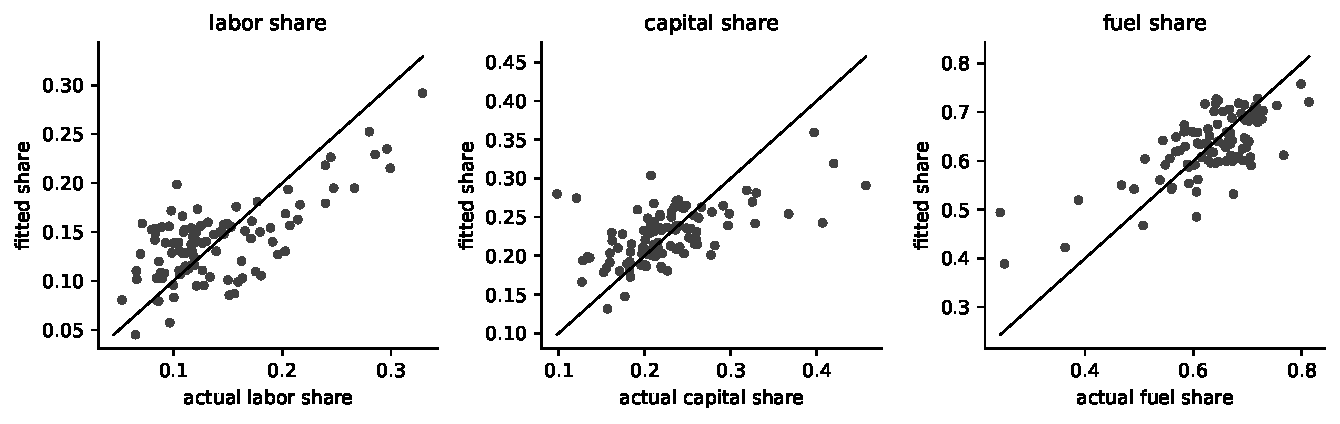
\includegraphics[width=0.95\textwidth]{figures/ch4_fitted_shares.pdf}
\end{center}
\begin{center}
\begin{minipage}{0.8\textwidth}\small
Figure S4.1: fitted versus actual cost shares in the constrained two-equation system (capital equation
dropped; fuel's fitted share computed as one minus the other two).  All fitted shares are positive ---
monotonicity holds in the relevant range --- and the fit is tightest for the dominant fuel share.
\end{minipage}
\end{center}

\begin{center}
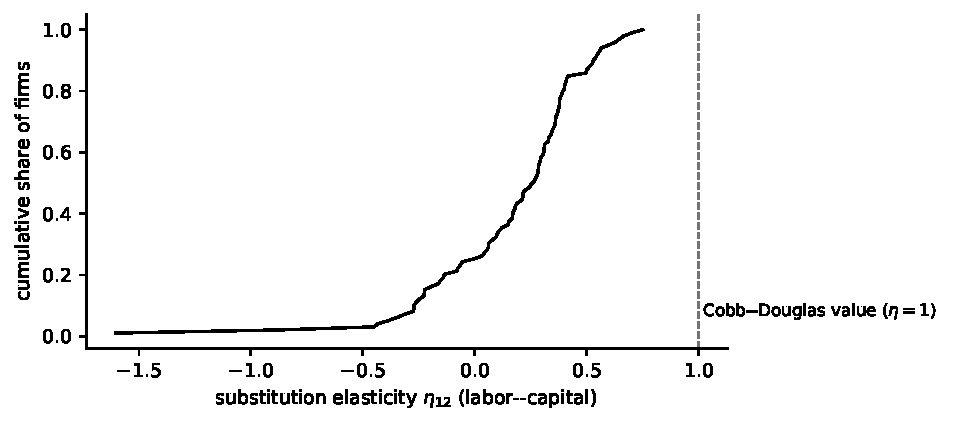
\includegraphics[width=0.62\textwidth]{figures/ch4_substitution.pdf}
\end{center}
\begin{center}
\begin{minipage}{0.8\textwidth}\small
Figure S4.2: empirical distribution of the labor--capital substitution elasticity $\eta_{12}$ of
\bk{(4.7.9)} evaluated at fitted shares across the 99 firms; the dashed line is the Cobb--Douglas value
$\eta=1$.  Every firm's elasticity is below unity, and most are far below.
\end{minipage}
\end{center}
\end{hee}


%% ========================================================================
\solchapter{5}{Panel Data}

\begin{center}
\begin{minipage}{0.86\textwidth}
\small
Solutions to all the exercises of Chapter 5 of Fumio Hayashi, \emph{Econometrics} (Princeton University
Press, 2000): the ten review questions of Sections 5.1--5.4, the seven analytical exercises, and the
empirical exercise on the Summers--Heston data.  Assumptions, propositions and equations cited as
\bk{Assumption 4.2}, \bk{Proposition 5.1} or \bk{(5.2.6)} refer to the book.  The numerical parts are
computed by \texttt{code/ch5.py}.
\end{minipage}
\end{center}

\bigskip
\hrule
\bigskip

\solsection{5.1}{The Error-Components Model}

\begin{hrq}{5.1.1}{}
Proposition 4.7 (efficient GMM for the multiple-equation model) requires: a system of $M$ linear
equations (\bk{(5.1.1)}), an ergodic stationary martingale-difference structure for
$\mathbf{g}_i\equiv\bs{\varepsilon}_i\otimes\mathbf{x}_i$ with a nonsingular long-run variance, an
identification (rank) condition, and conditional homoskedasticity.  Under \bk{(5.1.2)} the sample is
i.i.d., which is stronger than ergodic stationarity.  The orthogonality conditions \bk{(5.1.3)},
i.e.\ $\E(\mathbf{z}_{im}\varepsilon_{ih})=\mathbf{0}$ for all $m,h$, are exactly
$\E(\bs{\varepsilon}_i\otimes\mathbf{x}_i)=\mathbf{0}$, because $\mathbf{x}_i$ collects the unique
elements of $(\mathbf{z}_{i1},\dots,\mathbf{z}_{iM})$ and each $\varepsilon_{ih}$ is paired with every
element of $\mathbf{x}_i$ as $m$ and $h$ vary.  Therefore
$\E(\mathbf{g}_i\given\mathbf{g}_{i-1},\dots,\mathbf{g}_1)=\mathbf{0}$ by independence of
$\mathbf{g}_i$ from the past (i.i.d.\ sampling) and $\E(\mathbf{g}_i)=\mathbf{0}$:
$\{\mathbf{g}_i\}$ is a martingale difference sequence, and its long-run variance
$\mathbf{S}=\E(\mathbf{g}_i\mathbf{g}_i')$ is finite and nonsingular by \bk{(5.1.6)}.  The
identification condition is \bk{(5.1.4)}, assumed; conditional homoskedasticity is \bk{(5.1.5)}.
Thus all the hypotheses of Proposition 4.7 hold, and the random-effects estimator \bk{(4.6.8')}, which
is GMM with the efficient weighting matrix $\wh{\mathbf{S}}^{-1}$, is the efficient GMM estimator.

For the redundancy claim, recall from \bk{(4.6.16b)} the Kronecker-product expression: the
identification condition is that $\E(\mathbf{Z}_i\otimes\mathbf{x}_i)$ have full column rank $L$,
where $\mathbf{Z}_i$ is $M\times L$ and $\mathbf{x}_i$ is $K\times1$.  Since each row
$\mathbf{z}_{im}$ of $\mathbf{Z}_i$ is a subvector of $\mathbf{x}_i$, the matrix
$\mathbf{Z}_i\otimes\mathbf{x}_i$ is a fixed linear function of
$\mathbf{I}_M\otimes\mathbf{x}_i\mathbf{x}_i'$: stacking the columns,
$\vecop(\mathbf{Z}_i\otimes\mathbf{x}_i)=\mathbf{A}\,\vecop(\mathbf{I}_M\otimes
\mathbf{x}_i\mathbf{x}_i')$ for a constant selection matrix $\mathbf{A}$ of full column rank (each
column of $\mathbf{A}$ has a single nonzero element, different columns in different rows).  Taking
expectations,
\[
\E(\mathbf{Z}_i\otimes\mathbf{x}_i)=\mathbf{A}\,\E(\mathbf{I}_M\otimes
\mathbf{x}_i\mathbf{x}_i')=\mathbf{A}\bigl[\mathbf{I}_M\otimes\E(\mathbf{x}_i\mathbf{x}_i')\bigr].
\]
If $\E(\mathbf{x}_i\mathbf{x}_i')$ is nonsingular, so is
$\mathbf{I}_M\otimes\E(\mathbf{x}_i\mathbf{x}_i')$ (its eigenvalues are those of
$\E(\mathbf{x}_i\mathbf{x}_i')$, each repeated $M$ times); premultiplication by the full-column-rank
$\mathbf{A}$ then yields a matrix of full column rank $L$: the identification condition \bk{(5.1.4)}
holds automatically.  Since conditional homoskedasticity \bk{(5.1.5)} together with \bk{(5.1.6)}
implies \bk{(5.1.6')} --- $\bs{\Sigma}$ and $\E(\mathbf{x}_i\mathbf{x}_i')$ nonsingular --- the
separate identification assumption \bk{(5.1.4)} is implied by the other assumptions and is redundant
in the random-effects model.  (It is retained in the statement of the error-components model because
the \emph{fixed-effects} identification condition \bk{(5.1.15)} is \emph{not} redundant, as Review
Question 5.1.3 shows.)
\rmk{This is the panel-data analogue of the single-equation fact that, when the instruments are the
regressors themselves, nonsingularity of $\E(\mathbf{z}_i\mathbf{z}_i')$ delivers the GMM rank
condition.  Requiring $\E(\mathbf{x}_i\mathbf{x}_i')$ nonsingular for the union $\mathbf{x}_i$ of all
regressors is stronger than needed for \bk{(5.1.4)} alone, but it is exactly what \bk{(5.1.6')}
supplies.}
\end{hrq}

\begin{hrq}{5.1.2}{}
In the reparameterization \bk{(5.1.13)} the time-varying part is
\[
\mathbf{y}_i=\underbrace{\begin{bmatrix}1&0&S_{69i}\\ 0&1&S_{80i}\\ 0&0&S_{82i}\end{bmatrix}}_{\textstyle
\mathbf{F}_i^{(0)}}
\underbrace{\begin{bmatrix}\phi_1-\phi_3\\ \phi_2-\phi_3\\ \beta\end{bmatrix}}_{\textstyle
\bs{\beta}^{(0)}}
+\mathbf{1}_M\,\mathbf{b}_i'\bs{\gamma}+\mathbf{1}_M\alpha_i+\bs{\eta}_i,
\qquad
\mathbf{b}_i=\begin{bmatrix}1\\ \mathrm{IQ}_i\end{bmatrix},\quad
\bs{\gamma}=\begin{bmatrix}\phi_3\\ \gamma\end{bmatrix}.
\]
The proposed $\mathbf{F}_i$ replaces the first column $(1,0,0)'$ by $(1,-1,0)'$.  The two bases of the
same column space are related by
\[
\mathbf{F}_i=\mathbf{F}_i^{(0)}\mathbf{T},
\qquad
\mathbf{T}=\begin{bmatrix}1&0&0\\ -1&1&0\\ 0&0&1\end{bmatrix},
\qquad
\mathbf{T}^{-1}=\begin{bmatrix}1&0&0\\ 1&1&0\\ 0&0&1\end{bmatrix}.
\]
Since $\mathbf{F}_i\bs{\beta}=\mathbf{F}_i^{(0)}\mathbf{T}\bs{\beta}$ must equal
$\mathbf{F}_i^{(0)}\bs{\beta}^{(0)}$,
\[
\bs{\beta}=\mathbf{T}^{-1}\bs{\beta}^{(0)}
=\begin{bmatrix}\phi_1-\phi_3\\ (\phi_1-\phi_3)+(\phi_2-\phi_3)\\ \beta\end{bmatrix}
=\begin{bmatrix}\phi_1-\phi_3\\ \phi_1+\phi_2-2\phi_3\\ \beta\end{bmatrix},
\]
and $\delta$ stacks this $\bs{\beta}$ over the unchanged $\bs{\gamma}$:
$\delta=(\phi_1-\phi_3,\ \phi_1+\phi_2-2\phi_3,\ \beta,\ \phi_3,\ \gamma)'$,
with $\mathbf{b}_i=(1,\mathrm{IQ}_i)'$ unchanged.  The moral: fixed-effects estimation identifies only
the \emph{space} spanned by the time-varying regressors, so $\bs{\beta}$ is determined only up to
invertible reparameterization; which combination of the $\phi$'s is estimated depends on the arbitrary
choice of which intercept is folded into $\mathbf{b}_i$.  The fitted values $\mathbf{F}_i\bs{\beta}$,
and hence the estimator of any quantity invariant to the choice (such as the difference
$\phi_2-\phi_1$), are unique.
\end{hrq}

\begin{hrq}{5.1.3}{}
Condition \bk{(5.1.15)} requires $\E(\mathbf{Q}\mathbf{F}_i\otimes\mathbf{x}_i)$ to be of full column
rank, where
\[
\mathbf{x}_i=(1,S_{69i},S_{80i},S_{82i},\mathrm{IQ}_i)'.
\]
Premultiplication by
$\mathbf{Q}$ takes deviations from group means of each column of $\mathbf{F}_i$.  The first three
columns are the unit vectors $\mathbf{e}_1,\mathbf{e}_2,\mathbf{e}_3$, constant across $i$, so the
$m$-th column of $\mathbf{Q}\mathbf{F}_i$ is the constant vector $\mathbf{Q}\mathbf{e}_m$
($m=1,2,3$); the fourth is $(S_{69i}-\bar S_i,\,S_{80i}-\bar S_i,\,S_{82i}-\bar S_i)'$ with
$\bar S_i\equiv\frac13(S_{69i}+S_{80i}+S_{82i})$.  Consequently the block of
$\mathbf{Q}\mathbf{F}_i\otimes\mathbf{x}_i$ corresponding to column $m$ is
$\mathbf{Q}\mathbf{e}_m\otimes\mathbf{x}_i$, whose expectation is
$\mathbf{Q}\mathbf{e}_m\otimes\E(\mathbf{x}_i)$.  But the three constant vectors
$\mathbf{Q}\mathbf{e}_1,\mathbf{Q}\mathbf{e}_2,\mathbf{Q}\mathbf{e}_3$ are linearly dependent: they
sum to $\mathbf{Q}\mathbf{1}_M=\mathbf{0}$.  Hence
\[
\bigl[\mathbf{Q}\mathbf{e}_1\otimes\E(\mathbf{x}_i)\bigr]
+\bigl[\mathbf{Q}\mathbf{e}_2\otimes\E(\mathbf{x}_i)\bigr]
+\bigl[\mathbf{Q}\mathbf{e}_3\otimes\E(\mathbf{x}_i)\bigr]
=\mathbf{0}\otimes\E(\mathbf{x}_i)=\mathbf{0},
\]
a nontrivial linear relation among the column blocks of $\E(\mathbf{Q}\mathbf{F}_i\otimes
\mathbf{x}_i)$ (nontrivial because $\E(\mathbf{x}_i)\neq\mathbf{0}$ here: $\E S_{mi}>0$).  The matrix
is rank deficient and \bk{(5.1.15)} fails.  The economic content is immediate: three equation-specific
intercepts contain a common intercept in their span, and a common intercept is swept away by
$\mathbf{Q}$ together with the fixed effect and the common regressor IQ.  One of the three $\phi$'s is
simply not identified after the transformation; the two that remain must measure differences from the
third --- which is precisely what the reparameterization \bk{(5.1.13)} accomplishes.
\end{hrq}

\solsection{5.2}{The Fixed-Effects Estimator}

\begin{hrq}{5.2.1}{}
No.  The fixed-effects estimator is computed from the transformed system
$\wt{\mathbf{y}}_i=\wt{\mathbf{F}}_i\bs{\beta}+\wt{\bs{\eta}}_i$ with
$\wt{\bs{\eta}}_i=\mathbf{Q}\bs{\eta}_i$, and its sampling error \bk{(5.2.5)} is
\[
\wh{\bs{\beta}}_{\mathrm{FE}}-\bs{\beta}
=\Bigl(\frac1n\sum_{i=1}^n\mathbf{F}_i'\mathbf{Q}\mathbf{F}_i\Bigr)^{-1}
\frac1n\sum_{i=1}^n\mathbf{F}_i'\mathbf{Q}\bs{\eta}_i .
\]
Consistency and asymptotic normality (Proposition 5.1) require: (i) the identification condition
\bk{(5.1.15)}, which makes the first factor converge to a nonsingular matrix; (ii)
$\E(\mathbf{F}_i'\mathbf{Q}\bs{\eta}_i)=\mathbf{0}$, which follows from the orthogonality conditions
\bk{(5.2.6)} between the regressors and the \emph{second} error component alone; and (iii) a central
limit theorem for $\mathbf{F}_i'\mathbf{Q}\bs{\eta}_i$.  The fixed effect $\alpha_i$ has been swept
out by $\mathbf{Q}$ before any of these conditions is invoked, so no property of the joint
distribution of $(\alpha_i,\bs{\eta}_i)$ --- in particular not
$\E(\alpha_i\bs{\eta}_i)=\mathbf{0}$ --- is ever used.  This robustness to arbitrary correlation
between the individual effect and the idiosyncratic shock (and, more importantly, between the
individual effect and the regressors) is the whole point of the fixed-effects technique; it is what
the random-effects estimator, which treats $\mathbf{1}_M\alpha_i+\bs{\eta}_i$ as a composite error
term, does not deliver.
\end{hrq}

\begin{hrq}{5.2.2}{}
Let $\mathbf{C}'$ be the $(M-1)\times M$ matrix that keeps the first $M-1$ rows of $\mathbf{Q}$.
Dropping the last transformed equation for each group amounts to pooled OLS on the system
$\mathbf{C}'\mathbf{y}_i=\mathbf{C}'\mathbf{F}_i\bs{\beta}+\mathbf{C}'\bs{\eta}_i$, giving
\[
\wh{\bs{\beta}}_{\mathrm{drop}}
=\Bigl(\sum_{i=1}^n\mathbf{F}_i'\mathbf{C}\mathbf{C}'\mathbf{F}_i\Bigr)^{-1}
\sum_{i=1}^n\mathbf{F}_i'\mathbf{C}\mathbf{C}'\mathbf{y}_i .
\]
The fixed-effects estimator \bk{(5.2.4)} has $\mathbf{Q}$ in place of $\mathbf{C}\mathbf{C}'$, and
$\mathbf{C}\mathbf{C}'\neq\mathbf{Q}$: $\mathbf{C}\mathbf{C}'$ is $\mathbf{Q}$ with its last row and
column replaced by zeros (it projects onto the first $M-1$ coordinates of the deviation space and
annihilates the last), a matrix of rank $M-1$ that is not the annihilator.  For $M=2$ the distinction
happens to be immaterial --- the second transformed equation is minus the first, so both estimators
reduce to first-difference OLS --- but for $M\ge3$ they genuinely differ: the dropped-equation
estimator weights the $M-1$ retained deviations asymmetrically, and its probability limit involves a
different combination of the cross moments $\E(\mathbf{f}_{im}\eta_{ih})$.  The deeper point is that
the transformation must preserve the \emph{inner-product} structure that makes the estimator invariant
to which equation is treated as redundant; $\mathbf{Q}$ does (Analytical Exercise 5.2 shows that any
full-rank $\mathbf{C}$ with $\mathbf{C}'\mathbf{1}_M=\mathbf{0}$ works when paired with the weighting
$(\mathbf{C}'\mathbf{C})^{-1}$), but plain unweighted OLS on a strict subset of the equations does
not.
\rmk{This is also why the degrees-of-freedom correction in \bk{(5.2.17)} subtracts $n$ from $Mn$: the
$n$ linear constraints $\mathbf{1}_M'\wt{\mathbf{y}}_i=0$ make $n$ of the $Mn$ transformed
observations redundant, but they are redundant \emph{jointly}, not observation by observation, so one
cannot simply delete them before estimating.}
\end{hrq}

\begin{hrq}{5.2.3}{}
Consistency requires $\E(\mathbf{F}_i'\mathbf{Q}\bs{\eta}_i)=\mathbf{0}$.  Expanding with
$\mathbf{Q}=(q_{mh})$ (this is \bk{(4.6.16b)} in scalar form),
\[
\E(\mathbf{F}_i'\mathbf{Q}\bs{\eta}_i)
=\sum_{m=1}^M\sum_{h=1}^M q_{mh}\,\E(\mathbf{f}_{im}\eta_{ih}),
\]
a double sum over \emph{all} pairs $(m,h)$.  If only the own-equation orthogonalities
$\E(\mathbf{f}_{im}\eta_{im})=\mathbf{0}$ hold, the terms with $m\neq h$ survive: they are weighted by
$q_{mh}=-1/M\neq0$, and there is no reason for the off-diagonal sum to vanish.  Hence
\[
\plim\wh{\bs{\beta}}_{\mathrm{FE}}-\bs{\beta}
=\bigl[\E(\mathbf{F}_i'\mathbf{Q}\mathbf{F}_i)\bigr]^{-1}
\sum_{m\neq h}q_{mh}\,\E(\mathbf{f}_{im}\eta_{ih}),
\]
which is nonzero in general.  The fixed-effects estimator needs the regressors of \emph{every}
equation to be orthogonal to the error of \emph{every} equation, because the deviation-from-means
transformation mixes all $M$ equations: $\wt{\eta}_{im}=\eta_{im}-\frac1M\sum_h\eta_{ih}$ contains the
errors of all equations, and $\mathbf{f}_{im}$ must be orthogonal to each of them.  The dynamic panel
of Section 5.4 and Analytical Exercise 5.4 is the canonical example in which the cross
orthogonalities fail: $\E(y_{i,m-1}\eta_{ih})\neq0$ for $h\le m-1$, and the within estimator is
inconsistent however large $n$ is.
\end{hrq}

\begin{hrq}{5.2.4}{}
Since $\wt{\bs{\eta}}_i=\mathbf{Q}\bs{\eta}_i$ and $\mathbf{Q}\mathbf{1}_M=\mathbf{0}$,
\[
\mathbf{1}_M'\wt{\bs{\eta}}_i=\mathbf{1}_M'\mathbf{Q}\bs{\eta}_i
=(\mathbf{Q}\mathbf{1}_M)'\bs{\eta}_i=0
\quad\text{with probability one.}
\]
Hence
$\E(\wt{\bs{\eta}}_i\wt{\bs{\eta}}_i')\mathbf{1}_M
=\E\bigl[\wt{\bs{\eta}}_i(\mathbf{1}_M'\wt{\bs{\eta}}_i)'\bigr]=\mathbf{0}$: the vector
$\mathbf{1}_M$ lies in the null space, so the $M\times M$ matrix
$\E(\wt{\bs{\eta}}_i\wt{\bs{\eta}}_i')$ has rank at most $M-1$.  Equivalently,
$\E(\wt{\bs{\eta}}_i\wt{\bs{\eta}}_i')=\mathbf{Q}\E(\bs{\eta}_i\bs{\eta}_i')\mathbf{Q}$, and
$\rank(\mathbf{Q}\mathbf{A}\mathbf{Q})\le\rank(\mathbf{Q})=M-1$ for any $\mathbf{A}$.  The
transformed errors sum to zero within each group, so their covariance matrix must be singular.  What
matters for the asymptotic variance \bk{(5.2.7)} is that the singularity does not propagate:
$\E(\mathbf{F}_i'\mathbf{Q}\mathbf{F}_i)$ is nonsingular by \bk{(5.1.15)} (Analytical Exercise
5.5(a)), and the middle matrix of the sandwich is nonsingular by Analytical Exercise 5.5(b), so the
asymptotic variance itself is a positive definite $\#\bs{\beta}\times\#\bs{\beta}$ matrix.
\end{hrq}

\begin{hrq}{5.2.5}{}
Proposition 4.1 (consistent estimation of $\mathbf{S}$ from residuals) requires, for the transformed
system $\wt{\mathbf{y}}_i=\wt{\mathbf{F}}_i\bs{\beta}+\wt{\bs{\eta}}_i$: (i) an ergodic stationary
(or i.i.d.) sample; (ii) a consistent first-stage estimator $\wh{\bs{\beta}}$ with which to form
residuals $\wh{\wt{\bs{\eta}}}_i=\wt{\mathbf{y}}_i-\wt{\mathbf{F}}_i\wh{\bs{\beta}}$; (iii) finite
cross moments $\E(\wt{\eta}_{im}\wt{\mathbf{f}}_{ih}')$ and
$\E(\wt{\mathbf{f}}_{im}\wt{\mathbf{f}}_{ih}')$ (plus the usual finite fourth moments for the law of
large numbers applied to products); and (iv) the rank condition identifying $\bs{\beta}$.  Here: (i)
is \bk{(5.1.2)}; (ii) is supplied by the fixed-effects estimator itself, consistent under Proposition
5.1; (iv) is \bk{(5.1.15)}.  For (iii), write
$\wt{\mathbf{f}}_{im}=\sum_h q_{mh}\mathbf{f}_{ih}$ and $\wt{\eta}_{im}=\sum_h q_{mh}\eta_{ih}$: both
are fixed linear combinations (constant weights $q_{mh}$) of the elements of $\mathbf{F}_i$ and
$\bs{\eta}_i$, and $\mathbf{F}_i$ in turn collects elements of $\mathbf{x}_i$, as the hint notes.
The error-components model assumes $\E(\mathbf{x}_i\mathbf{x}_i')$ finite and nonsingular
(\bk{(5.1.5)} and \bk{(5.1.6)} imply \bk{(5.1.6')}) and
$\E(\bs{\eta}_i\bs{\eta}_i')$ finite (it is the $\eta\eta$ block of the assumed finite
$\bs{\Sigma}=\E(\bs{\varepsilon}_i\bs{\varepsilon}_i')$, since
$\bs{\varepsilon}_i=\mathbf{1}_M\alpha_i+\bs{\eta}_i$).  By Cauchy--Schwarz,
\[
\bigl|\E(\wt{\eta}_{im}\wt{f}_{ih,k})\bigr|
=\Bigl|\sum_{r,s}q_{mr}q_{hs}\,\E(\eta_{ir}f_{is,k})\Bigr|
\le\sum_{r,s}|q_{mr}q_{hs}|\,\sqrt{\E(\eta_{ir}^2)\,\E(f_{is,k}^2)}<\infty,
\]
since every $\E(\eta_{ir}^2)$ and $\E(f_{is,k}^2)$ is finite.  With all the conditions met,
Proposition 4.1 gives $\frac1n\sum_i\wh{\wt{\bs{\eta}}}_i\wh{\wt{\bs{\eta}}}_i'\convp
\E(\wt{\bs{\eta}}_i\wt{\bs{\eta}}_i')$, which is the consistency of \bk{(5.2.9)}, and plugging this
into \bk{(5.2.8)} yields a consistent estimator of the asymptotic variance of the fixed-effects
estimator.
\end{hrq}

\begin{hrq}{5.2.6}{}
No.  The random-effects estimator \bk{(4.6.8')} is GMM with weighting matrix built from
$\mathbf{S}=\bs{\Sigma}\otimes\E(\mathbf{x}_i\mathbf{x}_i')$; its probability limit is
\[
\plim\wh{\bs{\delta}}_{\mathrm{RE}}-\bs{\delta}
=\bigl[\E(\mathbf{Z}_i'\bs{\Sigma}^{-1}\mathbf{Z}_i)\bigr]^{-1}
\E(\mathbf{Z}_i'\bs{\Sigma}^{-1}\bs{\varepsilon}_i),
\]
so it is consistent if and only if
\[
\E(\mathbf{Z}_i'\bs{\Sigma}^{-1}\bs{\varepsilon}_i)=\mathbf{0},
\qquad \bs{\varepsilon}_i=\mathbf{1}_M\alpha_i+\bs{\eta}_i .
\]
Decompose:
\[
\E(\mathbf{Z}_i'\bs{\Sigma}^{-1}\bs{\varepsilon}_i)
=\E(\mathbf{Z}_i'\bs{\Sigma}^{-1}\mathbf{1}_M\alpha_i)
+\E(\mathbf{Z}_i'\bs{\Sigma}^{-1}\bs{\eta}_i).
\]
The second term vanishes when \bk{(5.1.8b)} holds: $\E(\mathbf{z}_{im}\eta_{ih})=0$ for all $m,h$
implies $\E(\mathbf{Z}_i'\mathbf{A}\bs{\eta}_i)=\mathbf{0}$ for any constant matrix $\mathbf{A}$, in
particular for $\mathbf{A}=\bs{\Sigma}^{-1}$.  So consistency fails if and only if
\[
\E(\mathbf{Z}_i'\bs{\Sigma}^{-1}\mathbf{1}_M\alpha_i)\neq\mathbf{0}.
\]
Condition \bk{(5.1.8a)} --- $\E(\mathbf{z}_{im}\alpha_i)=0$ for every $m$ --- is \emph{sufficient} for
this (it kills the first term whatever $\bs{\Sigma}$ is), but it is not \emph{necessary}: what is
required is only that the particular weighted combinations
$\sum_{m,h}(\bs{\Sigma}^{-1})_{mh}\,\E(\mathbf{z}_{im}\alpha_i)$ be zero, one vector equation in the
$M$ cross moments $\E(\mathbf{z}_{im}\alpha_i)$.  Those moments can all be nonzero --- \bk{(5.1.8a)}
failing in every equation --- and still conspire to satisfy the single effective restriction.  Thus,
strictly speaking, the Hausman test of Proposition 5.2 is not a test of \bk{(5.1.8a)}; it is a test of
$\E(\mathbf{Z}_i'\bs{\Sigma}^{-1}\bs{\varepsilon}_i)=\mathbf{0}$, the actual moment condition used by
the random-effects estimator.  The distinction rarely bites in practice --- for the weighted sum to
vanish while the individual moments do not is a measure-zero coincidence --- but it is the logically
correct statement of the null, and it is why the Hausman test is best described as a test of
\emph{overidentifying restrictions}: \bk{(5.1.8a)} is exactly the set of orthogonality conditions that
the random-effects estimator uses and the fixed-effects estimator does not.
\end{hrq}

\solsection{5.3}{Unbalanced Panels (optional)}

\begin{hrq}{5.3.1}{}
Here $M=3$ and $M_i=\mathbf{d}_i'\mathbf{d}_i=2$.  From \bk{(5.3.5)},
$\mathbf{Q}=\mathbf{I}_3-\frac1{M_i}\mathbf{d}_i\mathbf{d}_i'
=\mathbf{I}_3-\frac12\mathbf{d}_i\mathbf{d}_i'$, so
\[
\mathbf{Q}
=\begin{bmatrix}1&0&0\\ 0&1&0\\ 0&0&1\end{bmatrix}
-\frac12\begin{bmatrix}1&0&1\\ 0&0&0\\ 1&0&1\end{bmatrix}
=\begin{bmatrix}\frac12&0&-\frac12\\ 0&1&0\\ -\frac12&0&\frac12\end{bmatrix}.
\]
Check: $\mathbf{Q}\mathbf{d}_i=(\frac12-\frac12,\,0,\,-\frac12+\frac12)'=\mathbf{0}$, and $\mathbf{Q}$
is symmetric and idempotent --- it is the annihilator associated with $\mathbf{d}_i$.  Applied to
$\mathbf{y}_i=(y_{i1},0,y_{i3})'$ (the missing second observation zeroed out),
\[
\mathbf{Q}\mathbf{y}_i
=\bigl(\tfrac12(y_{i1}-y_{i3}),\,0,\,\tfrac12(y_{i3}-y_{i1})\bigr)'
=\bigl(y_{i1}-\bar y_i,\,0,\,y_{i3}-\bar y_i\bigr)',
\qquad \bar y_i=\tfrac{y_{i1}+y_{i3}}{2},
\]
so available observations enter as deviations from the mean \emph{over available observations}, and
the missing row stays zero --- exactly the ``zeroing out'' described in the text.  Verified
numerically in \texttt{code/ch5.py}.
\end{hrq}

\begin{hrq}{5.3.2}{}
Let $\mathbf{E}_i$ be the $M\times M_i$ selection matrix that picks out the observed rows, so
$\mathbf{y}_i^*=\mathbf{E}_i'\mathbf{y}_i$, $\mathbf{F}_i^*=\mathbf{E}_i'\mathbf{F}_i$,
$\mathbf{d}_i^*=\mathbf{E}_i'\mathbf{d}_i=\mathbf{1}_{M_i}$,
$\mathbf{E}_i'\mathbf{E}_i=\mathbf{I}_{M_i}$, and
$\mathbf{E}_i\mathbf{E}_i'=\diag(\mathbf{d}_i)$.  Because missing rows are zero-filled,
$\mathbf{d}_i=\mathbf{E}_i\mathbf{1}_{M_i}$ and
\[
\mathbf{F}_i'\mathbf{Q}\mathbf{F}_i
=\mathbf{F}_i'\Bigl(\mathbf{I}_M-\tfrac1{M_i}\mathbf{d}_i\mathbf{d}_i'\Bigr)\mathbf{F}_i
=\mathbf{F}_i'\mathbf{F}_i-\frac1{M_i}\bigl(\mathbf{E}_i'\mathbf{F}_i\bigr)'
\mathbf{1}_{M_i}\mathbf{1}_{M_i}'\bigl(\mathbf{E}_i'\mathbf{F}_i\bigr).
\]
Two substitutions finish the job: $\mathbf{E}_i'\mathbf{F}_i=\mathbf{F}_i^*$ by definition, and ---
this is where zeroing out is used --- $\mathbf{F}_i'\mathbf{F}_i=\mathbf{F}_i^{*\prime}\mathbf{F}_i^*$
because the rows of $\mathbf{F}_i$ corresponding to missing observations are all zeros and contribute
nothing to the cross-product.  Hence
\[
\mathbf{F}_i'\mathbf{Q}\mathbf{F}_i
=\mathbf{F}_i^{*\prime}\Bigl(\mathbf{I}_{M_i}-\frac1{M_i}\mathbf{1}_{M_i}\mathbf{1}_{M_i}'\Bigr)
\mathbf{F}_i^*
=\mathbf{F}_i^{*\prime}\mathbf{Q}^*\mathbf{F}_i^*,
\]
and by the identical computation
$\mathbf{F}_i'\mathbf{Q}\mathbf{y}_i=\mathbf{F}_i^{*\prime}\mathbf{Q}^*\mathbf{y}_i^*$.  Summing over
$i$ and inverting,
\[
\wh{\bs{\beta}}_{\mathrm{FE}}
=\Bigl(\sum_{i=1}^n\mathbf{F}_i^{*\prime}\mathbf{Q}^*\mathbf{F}_i^*\Bigr)^{-1}
\sum_{i=1}^n\mathbf{F}_i^{*\prime}\mathbf{Q}^*\mathbf{y}_i^*,
\]
which is \bk{(5.2.4)} written with the starred quantities: the ``compressed'' panel, with missing rows
deleted rather than zero-filled, delivers numerically the same estimator.  This is how panel software
actually computes the estimator; the zero-filled representation exists to give it the common matrix
form \bk{(5.2.4)} across balanced and unbalanced panels, which is what makes the proof of Proposition
5.4 run parallel to that of Proposition 5.1.
\end{hrq}

\begin{hrq}{5.3.3}{}
(a) Apply the zeroing-out device of \bk{(5.3.3)} to the levels system
$\mathbf{y}_i=\mathbf{Z}_i\bs{\delta}+\bs{\varepsilon}_i$: if observation $m$ of group $i$ is
missing, replace the $m$-th element of $\mathbf{y}_i$ and the $m$-th row of $\mathbf{Z}_i$ by zeros
(and likewise for $\bs{\varepsilon}_i$), keeping all matrices at their balanced-panel dimensions.
The estimator \bk{(4.6.11')} keeps its form,
\[
\wh{\bs{\delta}}
=\Bigl(\sum_{i=1}^n\mathbf{Z}_i'\mathbf{Z}_i\Bigr)^{-1}\sum_{i=1}^n\mathbf{Z}_i'\mathbf{y}_i
=\Bigl(\frac1n\sum_{i=1}^n\mathbf{Z}_i'\mathbf{Z}_i\Bigr)^{-1}
\frac1n\sum_{i=1}^n\mathbf{Z}_i'\mathbf{y}_i,
\]
understood with the zero-filled matrices: rows of zeros contribute nothing to either cross-product,
so this is exactly pooled OLS on the $\sum_i M_i$ available observations.  The orthogonality
conditions must be strengthened to rule out selectivity,
$\E(\mathbf{z}_{im}\varepsilon_{ih}\given\mathbf{d}_i)=\mathbf{0}$ for all $m,h$, exactly as
\bk{(5.3.7)} strengthens \bk{(5.2.6)}: sample selection must not depend on the error term.

(b) Substituting $\mathbf{y}_i=\mathbf{Z}_i\bs{\delta}+\bs{\varepsilon}_i$ gives the sampling error
$\wh{\bs{\delta}}-\bs{\delta}=\bigl(\frac1n\sum_i\mathbf{Z}_i'\mathbf{Z}_i\bigr)^{-1}
\frac1n\sum_i\mathbf{Z}_i'\bs{\varepsilon}_i$.  Without conditional homoskedasticity the middle
matrix does not collapse, so Kolmogorov's LLN and the Lindeberg--Levy CLT give
\[
\Avar\bigl(\sqrt n\,(\wh{\bs{\delta}}-\bs{\delta})\bigr)
=\bigl[\E(\mathbf{Z}_i'\mathbf{Z}_i)\bigr]^{-1}
\E\bigl(\mathbf{Z}_i'\bs{\varepsilon}_i\bs{\varepsilon}_i'\mathbf{Z}_i\bigr)
\bigl[\E(\mathbf{Z}_i'\mathbf{Z}_i)\bigr]^{-1},
\]
the displayed answer (with the book's tildes denoting the zero-filled quantities; the middle matrix
is the variance of $\mathbf{Z}_i'\bs{\varepsilon}_i$, finite under the usual fourth-moment
conditions).

(c) Mimic Proposition 5.3(b): replace the population moments by sample analogues computed from the
pooled residuals $\wh{\bs{\varepsilon}}_i=\mathbf{y}_i-\mathbf{Z}_i\wh{\bs{\delta}}$ (zero-filled in
the same way),
\[
\wh{\Avar}
=\Bigl(\frac1n\sum_{i=1}^n\mathbf{Z}_i'\mathbf{Z}_i\Bigr)^{-1}
\Bigl(\frac1n\sum_{i=1}^n\mathbf{Z}_i'\wh{\bs{\varepsilon}}_i\wh{\bs{\varepsilon}}_i'
\mathbf{Z}_i\Bigr)
\Bigl(\frac1n\sum_{i=1}^n\mathbf{Z}_i'\mathbf{Z}_i\Bigr)^{-1},
\]
which is the hint's instruction verbatim: replace $\mathbf{F}_i$ by $\mathbf{Z}_i$, $\mathbf{Q}$ by
$\mathbf{I}_M$, and $\wt{\bs{\eta}}_i$ by $\bs{\varepsilon}_i$ in \bk{(5.2.24)}.  Consistency follows
from Proposition 4.1 applied to this system, under the no-selectivity condition and finite fourth
moments.  Under conditional homoskedasticity the middle matrix simplifies and one recovers the
pooled-OLS formula of Section 4.6.
\end{hrq}

\solsection{5.4}{Application: International Differences in Growth Rates}

\begin{hrq}{5.4.1}{}
No.  Trace the derivation: \bk{(5.4.2)} gives
$\log q(t_m)=\rho\log q(t_{m-1})+(1-\rho)\log q^*$ with $\rho=\exp(-\lambda(t_m-t_{m-1}))$; with
$\log q(t)=\log(Y(t)/L(t))-\log A(0)-g\,t$ substituted in, the terms involving $g$ and $A(0)$
contribute
\[
-g\,t_m+\rho\,g\,t_{m-1}=-g\,(t_m-\rho\,t_{m-1}),
\]
which is absorbed into the intercept $\xi_m$ of \bk{(5.4.6)}, together with $(1-\rho)\log q^*$ and
the $\log A(0)$ pieces.  Suppose instead that technical progress grew at rate $g_m$ between $t_{m-1}$
and $t_m$, common across countries.  Then $A(t)$ cancels against the fixed effect and the common
trend in exactly the same way: the only change is that $\xi_m$ picks up a different additive
constant, $-g_m(t_m-\rho\,t_{m-1})$, in each period.  Since the $\xi_m$ are free, equation-specific
intercepts --- and the empirical exercise of Section 5.4(b) indeed includes 24 year dummies --- any
common time path of $g$ is absorbed without trace.  What cannot be relaxed is the cross-country
restriction: if $g$ differed across countries in a manner correlated with $y_{i,m-1}$, it would not
be absorbed into the common $\xi_m$ and would bias $\rho$ (a country-specific mean of $g$ reappears
inside the country effect $\alpha_i$ of \bk{(5.4.9)}, which is exactly why the fixed-effects
treatment of Section 5.4 is attractive).  Constancy of $g$ over time is not needed; commonality
across countries is.
\end{hrq}

\begin{hrq}{5.4.2}{}
(a) The system \bk{(5.4.11)} with $M=3$ consists of two equations,
\[
y_{i2}-y_{i1}=\xi_1+(y_{i1}-y_{i0})\rho+(\eta_{i2}-\eta_{i1}),\qquad
y_{i3}-y_{i2}=\xi_2+(y_{i2}-y_{i1})\rho+(\eta_{i3}-\eta_{i2}),
\]
with common coefficient $\rho$ and equation-specific intercepts.  In the notation of \bk{(4.6.1)}
set, with superscript ``lev'' for the levels,
\[
y_{i1}\equiv y_{i2}^{\mathrm{lev}}-y_{i1}^{\mathrm{lev}},\qquad
\mathbf{z}_{i1}=\bigl(1,\;0,\;y_{i1}^{\mathrm{lev}}-y_{i0}^{\mathrm{lev}}\bigr)',
\]
\[
y_{i2}\equiv y_{i3}^{\mathrm{lev}}-y_{i2}^{\mathrm{lev}},\qquad
\mathbf{z}_{i2}=\bigl(0,\;1,\;y_{i2}^{\mathrm{lev}}-y_{i1}^{\mathrm{lev}}\bigr)',\qquad
\bs{\delta}=(\xi_1,\xi_2,\rho)'.
\]
Then $\mathbf{z}_{i1}'\bs{\delta}=\xi_1+(y_{i1}^{\mathrm{lev}}-y_{i0}^{\mathrm{lev}})\rho$ and
$\mathbf{z}_{i2}'\bs{\delta}=\xi_2+(y_{i2}^{\mathrm{lev}}-y_{i1}^{\mathrm{lev}})\rho$, as required:
the system is \bk{(4.6.1)} with $M=2$ equations and $L=3$ coefficients, and the second regressor
vector is the hint's $(0,1,y_{i2}-y_{i1})'$.

(b) With instruments $\mathbf{x}_{im}=(1,s_{im})'$, the instrument vector for the system is
$\mathbf{x}_i=(1,s_{i1},s_{i2})'$ ($K=3$ unique elements).  Identification for the
multiple-equation GMM requires $\E(\mathbf{Z}_i\otimes\mathbf{x}_i)$ to have full column rank $L=3$.
Examine the column of this matrix associated with $\rho$: its nonzero elements are
$\E[(y_{i1}-y_{i0})\mathbf{x}_{i1}]$ from equation 1 and $\E[(y_{i2}-y_{i1})\mathbf{x}_{i2}]$ from
equation 2.  Suppose $\Cov(s_{im},y_{im}-y_{i,m-1})=0$ for $m=1,2$, i.e.\
$\E[s_{im}(y_{im}-y_{i,m-1})]=\E(s_{im})\,\E(y_{im}-y_{i,m-1})$.  Then
\[
\E\bigl[(y_{im}-y_{i,m-1})\mathbf{x}_{im}\bigr]
=\E(y_{im}-y_{i,m-1})\cdot\bigl(1,\E(s_{im})\bigr)'
=\E(y_{im}-y_{i,m-1})\cdot\E(\mathbf{x}_{im}),
\]
so the $\rho$ column of $\E(\mathbf{Z}_i\otimes\mathbf{x}_i)$ satisfies
\[
\mathrm{col}_{\rho}
=\E(y_{i1}-y_{i0})\cdot\mathrm{col}_{\xi_1}
+\E(y_{i2}-y_{i1})\cdot\mathrm{col}_{\xi_2},
\]
because the intercept columns contribute the blocks
$(\E(\mathbf{x}_{i1}'),\mathbf{0}')'$ and $(\mathbf{0}',\E(\mathbf{x}_{i2}'))'$ respectively.  A
nontrivial linear combination of the columns is zero, so the rank is at most $2<3$: the rank
condition fails and $\rho$ is not identified.  The economics is transparent: in each differenced
equation the only instrument capable of separating $\rho$ from the intercept is the saving rate, and
if the saving rate does not covary with the contemporaneous change in log output it has no power to
do so; each equation collapses to a reduced-form mean.  Instrument \emph{relevance}
($\Cov\neq0$) is indispensable on top of instrument exogeneity.
\end{hrq}

\problemset{5}{Problem Set for Chapter 5: Analytical Exercises}

\begin{hax}{5.1}{}
(a) \emph{First proof (Frisch--Waugh).}  By the Frisch--Waugh theorem (Analytical Exercise 1.4(b)),
the OLS coefficient on $\mathbf{F}$ in the regression of $\mathbf{y}$ on
$\mathbf{W}=(\mathbf{D}\;\;\mathbf{F})$ equals the OLS coefficient in the regression of
$\mathbf{M}_{\mathbf{D}}\mathbf{y}$ on $\mathbf{M}_{\mathbf{D}}\mathbf{F}$, where
$\mathbf{M}_{\mathbf{D}}=\mathbf{I}_{Mn}-\mathbf{D}(\mathbf{D}'\mathbf{D})^{-1}\mathbf{D}'$.  Since
$\mathbf{D}=\mathbf{I}_n\otimes\mathbf{1}_M$,
\[
\mathbf{D}'\mathbf{D}=\mathbf{I}_n\otimes(\mathbf{1}_M'\mathbf{1}_M)=M\,\mathbf{I}_n,
\qquad
\mathbf{D}(\mathbf{D}'\mathbf{D})^{-1}\mathbf{D}'
=\mathbf{I}_n\otimes\tfrac1M\mathbf{1}_M\mathbf{1}_M',
\]
so
\[
\mathbf{M}_{\mathbf{D}}
=\mathbf{I}_n\otimes\Bigl(\mathbf{I}_M-\tfrac1M\mathbf{1}_M\mathbf{1}_M'\Bigr)
=\mathbf{I}_n\otimes\mathbf{Q},
\]
with $\mathbf{Q}$ the annihilator associated with $\mathbf{1}_M$.  Hence
$\mathbf{M}_{\mathbf{D}}\mathbf{F}$ stacks the blocks
$\mathbf{Q}\mathbf{F}_i=\wt{\mathbf{F}}_i$ and $\mathbf{M}_{\mathbf{D}}\mathbf{y}$ stacks
$\mathbf{Q}\mathbf{y}_i=\wt{\mathbf{y}}_i$, and the coefficient is
\[
\mathbf{b}
=\bigl[(\mathbf{M}_{\mathbf{D}}\mathbf{F})'(\mathbf{M}_{\mathbf{D}}\mathbf{F})\bigr]^{-1}
(\mathbf{M}_{\mathbf{D}}\mathbf{F})'\mathbf{M}_{\mathbf{D}}\mathbf{y}
=\Bigl(\sum_{i=1}^n\mathbf{F}_i'\mathbf{Q}\mathbf{F}_i\Bigr)^{-1}
\sum_{i=1}^n\mathbf{F}_i'\mathbf{Q}\mathbf{y}_i
=\wh{\bs{\beta}}_{\mathrm{FE}},
\]
using symmetry and idempotency of $\mathbf{M}_{\mathbf{D}}$; this is exactly \bk{(5.2.4)}.

\emph{Second proof (normal equations).}  The normal equations
$\mathbf{W}'\mathbf{W}\bigl[\begin{smallmatrix}\wh{\bs{\alpha}}\\ \mathbf{b}\end{smallmatrix}\bigr]
=\mathbf{W}'\mathbf{y}$ in partitioned form are
\[
\mathbf{D}'\mathbf{D}\,\wh{\bs{\alpha}}+\mathbf{D}'\mathbf{F}\mathbf{b}=\mathbf{D}'\mathbf{y},
\qquad
\mathbf{F}'\mathbf{D}\,\wh{\bs{\alpha}}+\mathbf{F}'\mathbf{F}\mathbf{b}=\mathbf{F}'\mathbf{y}.
\]
The first gives $\wh{\bs{\alpha}}=(\mathbf{D}'\mathbf{D})^{-1}(\mathbf{D}'\mathbf{y}
-\mathbf{D}'\mathbf{F}\mathbf{b})$, the formula suggested in the hint.  Substituting into the
second,
\[
\mathbf{F}'\bigl[\mathbf{I}-\mathbf{D}(\mathbf{D}'\mathbf{D})^{-1}\mathbf{D}'\bigr]\mathbf{F}
\,\mathbf{b}
=\mathbf{F}'\bigl[\mathbf{I}-\mathbf{D}(\mathbf{D}'\mathbf{D})^{-1}\mathbf{D}'\bigr]\mathbf{y},
\]
i.e.\ $\mathbf{F}'\mathbf{M}_{\mathbf{D}}\mathbf{F}\,\mathbf{b}
=\mathbf{F}'\mathbf{M}_{\mathbf{D}}\mathbf{y}$, the same system as above.  The inversion is trivial
because $\mathbf{D}'\mathbf{D}=M\mathbf{I}_n$ --- which is why the dummy-variable route is
computationally painless even with thousands of groups.

(b) Row $i$ of the first block of normal equations: the $i$-th diagonal block of
$\mathbf{D}'\mathbf{D}$ is $M$, the $i$-th block of $\mathbf{D}'\mathbf{y}$ is
$\mathbf{1}_M'\mathbf{y}_i=M\bar y_i$, and the $i$-th block of $\mathbf{D}'\mathbf{F}$ is
$\mathbf{1}_M'\mathbf{F}_i=M\bar{\mathbf{f}}_i'$.  Hence
\[
M\,\wh{\alpha}_i+M\,\bar{\mathbf{f}}_i'\mathbf{b}=M\bar y_i
\quad\Longrightarrow\quad
\wh{\alpha}_i=\bar y_i-\bar{\mathbf{f}}_i'\mathbf{b},
\]
which is the displayed result: the estimated fixed effect is what remains of the group's mean
dependent variable after subtracting the systematic part fitted at the group's mean regressors.

(c) \emph{Classical assumptions.}  Linearity (Assumption 1.1) holds by construction, with the
coefficient vector $(\bs{\alpha}',\bs{\beta}')'$ common to all $Mn$ observations.  For strict
exogeneity (Assumption 1.2), note that $\mathbf{D}$ is a matrix of constants, so conditioning on
$\mathbf{W}=(\mathbf{D}\;\;\mathbf{F})$ is conditioning on
$\mathbf{F}=(\mathbf{F}_1',\dots,\mathbf{F}_n')'$:
\[
\E(\bs{\eta}_i\given\mathbf{W})=\E(\bs{\eta}_i\given\mathbf{F})
=\E(\bs{\eta}_i\given\mathbf{F}_i)=\mathbf{0},
\]
the second equality because $\bs{\eta}_i$ is independent of
$(\mathbf{F}_1,\dots,\mathbf{F}_{i-1},\mathbf{F}_{i+1},\dots,\mathbf{F}_n)$ by the i.i.d.\
assumption (i), the third by (ii).  Conditional homoskedasticity (Assumption 1.4):
\[
\E(\bs{\eta}_i\bs{\eta}_i'\given\mathbf{W})
=\E(\bs{\eta}_i\bs{\eta}_i'\given\mathbf{F}_i)=\sigma_\eta^2\mathbf{I}_M
\]
by the same independence and (iii); and $\E(\bs{\eta}_i\bs{\eta}_j'\given\mathbf{W})=\mathbf{0}$
for $i\neq j$ by (i) together with $\E(\bs{\eta}_i\given\mathbf{F})=\mathbf{0}$.  Stacking gives
$\E(\bs{\eta}\bs{\eta}'\given\mathbf{W})=\sigma_\eta^2\mathbf{I}_{Mn}$.  No multicollinearity
(Assumption 1.3) is (iv).  (If in addition $\bs{\eta}$ is normal, Assumption 1.5 holds too.)

\emph{Small-sample theory.}  All of Chapter 1's finite-sample results therefore apply to the pooled
regression: by Proposition 1.1, $(\wh{\bs{\alpha}},\mathbf{b})$ are unbiased conditional on
$\mathbf{W}$ (hence unconditionally), with
\[
\Var\Bigl(\begin{bmatrix}\wh{\bs{\alpha}}\\ \mathbf{b}\end{bmatrix}\Bigm|\mathbf{W}\Bigr)
=\sigma_\eta^2(\mathbf{W}'\mathbf{W})^{-1},
\]
and they are Gauss--Markov efficient in the class of linear unbiased estimators; under normality
the usual $t$ and $F$ tests are exact.  Two caveats.  First, unbiasedness uses strict exogeneity
\emph{with respect to the whole matrix $\mathbf{F}$} --- assumption (ii), which is stronger than
the orthogonality conditions \bk{(5.2.6)} that suffice for the large-sample theory, and which fails
in dynamic panels.  Second, with $n$ large and $M$ fixed, each $\wh{\alpha}_i$ is computed from
only $M$ observations and is not consistent as $n\to\infty$ (the incidental-parameters problem);
only $\mathbf{b}$ is consistent.

\emph{The $\SSR$.}  Yes, the two sums of squared residuals are identical.  By Frisch--Waugh
(Analytical Exercise 1.4(c)), the residual vector of the pooled regression equals the residual
vector of the regression of $\mathbf{M}_{\mathbf{D}}\mathbf{y}$ on
$\mathbf{M}_{\mathbf{D}}\mathbf{F}$, which is the within regression \bk{(5.2.15)}: the $i$-th block
is $\mathbf{Q}\mathbf{y}_i-\mathbf{Q}\mathbf{F}_i\mathbf{b}$.  Hence
$\SSR=\sum_i(\mathbf{Q}\mathbf{y}_i-\mathbf{Q}\mathbf{F}_i\mathbf{b})'
(\mathbf{Q}\mathbf{y}_i-\mathbf{Q}\mathbf{F}_i\mathbf{b})$, exactly \bk{(5.2.15)}.  (What differs
is only the degrees-of-freedom bookkeeping: the pooled regression estimates
$n+\#\bs{\beta}$ coefficients, so its $s^2$ divides by $Mn-n-\#\bs{\beta}$ --- which is the
\emph{correct} denominator \bk{(5.2.17)}.  The dummy-variable route gets the degrees-of-freedom
correction right automatically.)
\end{hax}

\begin{hax}{5.2}{}
(a) \emph{First-difference matrix.}  Let $\mathbf{C}$ be the $M\times(M-1)$ matrix with
$C_{m,m}=-1$, $C_{m+1,m}=1$ and zeros elsewhere, so $\mathbf{C}'\mathbf{y}_i$ stacks the first
differences $y_{i,m+1}-y_{im}$.  Column $m$ of $\mathbf{C}$ is $-\mathbf{e}_m+\mathbf{e}_{m+1}$,
whose elements sum to zero: $\mathbf{C}'\mathbf{1}_M=\mathbf{0}$.  Its $M-1$ columns are linearly
independent: if $\mathbf{C}\mathbf{c}=\mathbf{0}$, reading the rows from the top gives $-c_1=0$,
$c_1-c_2=0$, \dots, forcing $\mathbf{c}=\mathbf{0}$.  So $\mathbf{C}$ has full column rank $M-1$.

\emph{Dropped column of $\mathbf{Q}$.}  Write $\mathbf{Q}=(\mathbf{C}\;\;\mathbf{q})$ with
$\mathbf{C}$ the first $M-1$ columns.  Since $\mathbf{Q}\mathbf{1}_M=\mathbf{0}$, every column of
$\mathbf{Q}$ is orthogonal to $\mathbf{1}_M$, so $\mathbf{C}'\mathbf{1}_M=\mathbf{0}$.  The null
space of the symmetric idempotent $\mathbf{Q}$ is spanned by $\mathbf{1}_M$; if the first $M-1$
columns were linearly dependent, some $\mathbf{c}\neq\mathbf{0}$ supported on the first $M-1$
coordinates would satisfy $\mathbf{Q}\mathbf{c}=\mathbf{0}$, forcing
$\mathbf{c}\propto\mathbf{1}_M$ --- impossible for a vector with a zero last coordinate.  Hence
$\rank(\mathbf{C})=M-1$.

(b) Premultiplying \bk{(5.1.1'')},
$\mathbf{y}_i=\mathbf{F}_i\bs{\beta}+\mathbf{1}_M(\mathbf{b}_i'\bs{\gamma}+\alpha_i)
+\bs{\eta}_i$, by $\mathbf{C}'$ annihilates the $\mathbf{1}_M$ term because
$\mathbf{C}'\mathbf{1}_M=\mathbf{0}$:
\[
\mathbf{C}'\mathbf{y}_i=\mathbf{C}'\mathbf{F}_i\bs{\beta}+\mathbf{C}'\bs{\eta}_i,
\]
which is the transformed system with the stated definitions.  Note that both the fixed effect
\emph{and} the common regressors $\mathbf{b}_i$ drop out, since both enter through $\mathbf{1}_M$.

(c) Check the five assumptions of the random-effects model for the $(M-1)$-equation system.

\emph{Random sample:} $(\wt{\mathbf{y}}_i,\wt{\mathbf{F}}_i)$ is a fixed linear function of
$(\mathbf{y}_i,\mathbf{Z}_i)$, hence i.i.d.\ by \bk{(5.1.2)}.

\emph{Orthogonality conditions} $\E(\wt{\bs{\eta}}_i\otimes\mathbf{x}_i)=\mathbf{0}$: since
$\wt{\bs{\eta}}_i\otimes\mathbf{x}_i=(\mathbf{C}'\otimes\mathbf{I}_K)
(\bs{\eta}_i\otimes\mathbf{x}_i)$ and \bk{(5.1.8b)} is
$\E(\bs{\eta}_i\otimes\mathbf{x}_i)=\mathbf{0}$, the transformed moment is
$(\mathbf{C}'\otimes\mathbf{I}_K)\mathbf{0}=\mathbf{0}$.

\emph{Identification:} $\E(\wt{\mathbf{F}}_i\otimes\mathbf{x}_i)$ of full column rank is
equivalent to \bk{(5.1.15)}.  Indeed, with
$\mathbf{L}\equiv\mathbf{C}(\mathbf{C}'\mathbf{C})^{-1}$ the identity of part (d) gives
$\mathbf{Q}=\mathbf{L}\mathbf{C}'$, hence
$\E(\mathbf{Q}\mathbf{F}_i\otimes\mathbf{x}_i)
=(\mathbf{L}\otimes\mathbf{I}_K)\,\E(\mathbf{C}'\mathbf{F}_i\otimes\mathbf{x}_i)$; write this as
$\mathbf{A}=\mathbf{D}\mathbf{B}$ with $\mathbf{D}=\mathbf{L}\otimes\mathbf{I}_K$ of full column
rank.  Then $\rank(\mathbf{A})\le\rank(\mathbf{B})$, and
$\mathbf{D}'\mathbf{A}=(\mathbf{D}'\mathbf{D})\mathbf{B}$ with $\mathbf{D}'\mathbf{D}$ nonsingular,
so $\rank(\mathbf{A})\ge\rank(\mathbf{B})$: the ranks coincide, and since $\mathbf{A}$ and
$\mathbf{B}$ have the same number of columns, one has full column rank iff the other does.  (This
is the argument of the book's answer sheet.)

\emph{Conditional homoskedasticity:}
\[
\E(\wt{\bs{\eta}}_i\wt{\bs{\eta}}_i'\given\mathbf{x}_i)
=\mathbf{C}'\E(\bs{\varepsilon}_i\bs{\varepsilon}_i'\given\mathbf{x}_i)\mathbf{C}
=\mathbf{C}'\bs{\Sigma}\mathbf{C}\equiv\bs{\Psi},
\]
using $\wt{\bs{\eta}}_i=\mathbf{C}'\bs{\eta}_i=\mathbf{C}'\bs{\varepsilon}_i$ (because
$\mathbf{C}'\mathbf{1}_M\alpha_i=\mathbf{0}$) and \bk{(5.1.5)}; $\bs{\Psi}$ does not depend on
$\mathbf{x}_i$, and it is nonsingular because $\mathbf{C}$ has full column rank and $\bs{\Sigma}$
is positive definite (for $\mathbf{v}\neq\mathbf{0}$, $\mathbf{C}\mathbf{v}\neq\mathbf{0}$, so
$\mathbf{v}'\mathbf{C}'\bs{\Sigma}\mathbf{C}\mathbf{v}>0$).

\emph{Nonsingularity of $\E(\mathbf{g}_i\mathbf{g}_i')$:} with
$\mathbf{g}_i=\wt{\bs{\eta}}_i\otimes\mathbf{x}_i$,
\[
\E(\mathbf{g}_i\mathbf{g}_i')
=\E\bigl[\E(\wt{\bs{\eta}}_i\wt{\bs{\eta}}_i'\given\mathbf{x}_i)\otimes
\mathbf{x}_i\mathbf{x}_i'\bigr]
=\bs{\Psi}\otimes\E(\mathbf{x}_i\mathbf{x}_i'),
\]
nonsingular as the Kronecker product of two nonsingular matrices (the second factor nonsingular by
\bk{(5.1.6')}).  All five assumptions hold, so Proposition 4.7 applies to the transformed system.

(d) Use the hint's identity:
\[
\mathbf{Q}=\mathbf{C}(\mathbf{C}'\mathbf{C})^{-1}\mathbf{C}'
\qquad\text{for any } \mathbf{C} \text{ of full column rank with }
\mathbf{C}'\mathbf{1}_M=\mathbf{0}. \tag{$\ast$}
\]
(Proof: $\mathbf{C}(\mathbf{C}'\mathbf{C})^{-1}\mathbf{C}'$ is the orthogonal projector onto the
column space of $\mathbf{C}$; that space is contained in $\{\mathbf{1}_M\}^\perp$ because
$\mathbf{C}'\mathbf{1}_M=\mathbf{0}$, and it has dimension $M-1=\dim\{\mathbf{1}_M\}^\perp$, so it
equals $\{\mathbf{1}_M\}^\perp$; $\mathbf{Q}$ is the orthogonal projector onto the same space, and
orthogonal projectors onto a given subspace are unique.)  Substituting into \bk{(5.2.4)},
\[
\wh{\bs{\beta}}_{\mathrm{FE}}
=\Bigl(\frac1n\sum_i\wt{\mathbf{F}}_i'(\mathbf{C}'\mathbf{C})^{-1}\wt{\mathbf{F}}_i\Bigr)^{-1}
\frac1n\sum_i\wt{\mathbf{F}}_i'(\mathbf{C}'\mathbf{C})^{-1}\wt{\mathbf{y}}_i .
\]
This is the GMM format with, as the book says, ``the disappearance of $\mathbf{x}$'': the elements
of $\mathbf{F}_i$ being a subset of $\mathbf{x}_i$, the moment conditions that survive the
transformation are just the own-equation ones, and
\[
\mathbf{S}_{\mathbf{x}\mathbf{z}}=\frac1n\sum_{i=1}^n\wt{\mathbf{F}}_i,\qquad
\mathbf{s}_{\mathbf{x}y}=\frac1n\sum_{i=1}^n\wt{\mathbf{y}}_i,\qquad
\wh{\mathbf{W}}=(\mathbf{C}'\mathbf{C})^{-1}.
\]
So the fixed-effects estimator is GMM on the transformed system with weighting matrix
$(\mathbf{C}'\mathbf{C})^{-1}$ --- efficient if and only if $\bs{\Psi}$ is proportional to
$\mathbf{C}'\mathbf{C}$.

(e) All assumptions of Proposition 4.7 hold for the transformed system by part (c), so the
efficient GMM estimator uses $\wh{\mathbf{W}}=\wh{\bs{\Psi}}^{-1}$:
\[
\wh{\bs{\beta}}_{\mathrm{eff}}
=\Bigl(\sum_i\wt{\mathbf{F}}_i'\wh{\bs{\Psi}}^{-1}\wt{\mathbf{F}}_i\Bigr)^{-1}
\sum_i\wt{\mathbf{F}}_i'\wh{\bs{\Psi}}^{-1}\wt{\mathbf{y}}_i,
\qquad
\Avar\bigl(\sqrt n\,(\wh{\bs{\beta}}_{\mathrm{eff}}-\bs{\beta})\bigr)
=\bigl[\E(\wt{\mathbf{F}}_i'\bs{\Psi}^{-1}\wt{\mathbf{F}}_i)\bigr]^{-1},
\]
which is \bk{(13)}.  Comparing with the sandwich form of Proposition 5.1 confirms the text's
suspicion: the fixed-effects estimator is generally inefficient because it uses
$(\mathbf{C}'\mathbf{C})^{-1}$ where $\bs{\Psi}^{-1}$ belongs; the two coincide only when
$\bs{\Psi}\propto\mathbf{C}'\mathbf{C}$, which part (h) ties to sphericity.

(f) Let $\wh{\wt{\bs{\eta}}}_i=\wt{\mathbf{y}}_i-\wt{\mathbf{F}}_i\wh{\bs{\beta}}_{\mathrm{FE}}$
and write
\[
\wh{\bs{\Psi}}-\bs{\Psi}
=\frac1n\sum_i\bigl(\wt{\bs{\eta}}_i\wt{\bs{\eta}}_i'-\bs{\Psi}\bigr)
+\frac1n\sum_i\bigl(\wh{\wt{\bs{\eta}}}_i\wh{\wt{\bs{\eta}}}_i'
-\wt{\bs{\eta}}_i\wt{\bs{\eta}}_i'\bigr).
\]
The first term is $o_p(1)$ by Kolmogorov's LLN (i.i.d.\ sampling, finite
$\E\|\wt{\bs{\eta}}_i\|^2$ from finiteness of $\bs{\Sigma}$).  For the second, since
$\wh{\wt{\bs{\eta}}}_i=\wt{\bs{\eta}}_i-\wt{\mathbf{F}}_i(\wh{\bs{\beta}}_{\mathrm{FE}}
-\bs{\beta})$,
\[
\frac1n\sum_i\bigl(\wh{\wt{\bs{\eta}}}_i\wh{\wt{\bs{\eta}}}_i'
-\wt{\bs{\eta}}_i\wt{\bs{\eta}}_i'\bigr)
=-\Bigl(\frac1n\sum_i\wt{\bs{\eta}}_i\otimes\wt{\mathbf{F}}_i\Bigr)'_{\!\!(\cdot)}
(\wh{\bs{\beta}}_{\mathrm{FE}}-\bs{\beta})-\{\text{transpose}\}
+\frac1n\sum_i\wt{\mathbf{F}}_i(\wh{\bs{\beta}}_{\mathrm{FE}}-\bs{\beta})
(\wh{\bs{\beta}}_{\mathrm{FE}}-\bs{\beta})'\wt{\mathbf{F}}_i' ,
\]
where the sample moments converge by the LLN under the finite cross-moment conditions verified in
Review Question 5.2.5, while $\wh{\bs{\beta}}_{\mathrm{FE}}-\bs{\beta}=o_p(1)$ by Proposition 5.1.
So the whole expression is $o_p(1)$: these are exactly the conditions of Proposition 4.1 applied to
the transformed system, and $\wh{\bs{\Psi}}\convp\bs{\Psi}$.

(g) Sargan's statistic for the efficient estimator is \bk{(4.6.10')} applied to the transformed
system: with $\wh{\mathbf{g}}_i=\wh{\wt{\bs{\eta}}}_i\otimes\mathbf{x}_i$ evaluated at
$\wh{\bs{\beta}}_{\mathrm{eff}}$, $\wh{\mathbf{S}}=\frac1n\sum_i\wh{\mathbf{g}}_i
\wh{\mathbf{g}}_i'$ and $\bar{\mathbf{g}}_n=\frac1n\sum_i\wh{\mathbf{g}}_i$,
\[
J=n\,\bar{\mathbf{g}}_n'\wh{\mathbf{S}}^{-1}\bar{\mathbf{g}}_n
\convd\chi^2\bigl((M-1)K-\#\bs{\beta}\bigr),
\]
the degrees of freedom being the number of overidentifying restrictions: $(M-1)K$ moment
conditions minus $\#\bs{\beta}$ parameters.  (With the collapsed instruments of part (d) the
degrees of freedom reduce accordingly; the full instrument set tests the cross-equation
orthogonality conditions as well, which is what makes the statistic useful as a specification
test.)

(h) If $\bs{\eta}_i$ is spherical, $\E(\bs{\eta}_i\bs{\eta}_i')=\sigma_\eta^2\mathbf{I}_M$, then
\[
\bs{\Psi}=\mathbf{C}'\E(\bs{\eta}_i\bs{\eta}_i')\mathbf{C}=\sigma_\eta^2\,\mathbf{C}'\mathbf{C},
\]
so $\wh{\bs{\Psi}}=\wh{\sigma}_\eta^2\mathbf{C}'\mathbf{C}$ is consistent whenever
$\wh{\sigma}_\eta^2$ is (for instance Analytical Exercise 5.3's
$\SSR/[n(M-1)-\#\bs{\beta}]$).  The efficient GMM estimator with this weighting is
\[
\Bigl(\sum_i\wt{\mathbf{F}}_i'\bigl[\wh{\sigma}_\eta^2\mathbf{C}'\mathbf{C}\bigr]^{-1}
\wt{\mathbf{F}}_i\Bigr)^{-1}
\sum_i\wt{\mathbf{F}}_i'\bigl[\wh{\sigma}_\eta^2\mathbf{C}'\mathbf{C}\bigr]^{-1}
\wt{\mathbf{y}}_i
=\Bigl(\sum_i\mathbf{F}_i'\mathbf{C}(\mathbf{C}'\mathbf{C})^{-1}\mathbf{C}'\mathbf{F}_i\Bigr)^{-1}
\sum_i\mathbf{F}_i'\mathbf{C}(\mathbf{C}'\mathbf{C})^{-1}\mathbf{C}'\mathbf{y}_i,
\]
the scalar $\wh{\sigma}_\eta^2$ cancelling between the two factors; by $(\ast)$ this is exactly
$\wh{\bs{\beta}}_{\mathrm{FE}}$.  So \emph{under sphericity the fixed-effects estimator is the
efficient GMM estimator}: its inefficiency in Proposition 5.1 comes entirely from nonspherical
$\bs{\eta}_i$ (serial correlation or heteroskedasticity across $m$), and the estimator of part (e)
is the asymptotically more efficient estimator the text promised.

(i) Let $\mathbf{B}=\mathbf{C}\mathbf{A}$ with $\mathbf{A}$ an $(M-1)\times(M-1)$ nonsingular
matrix.  Then $\mathbf{B}'\mathbf{1}_M=\mathbf{A}'\mathbf{C}'\mathbf{1}_M=\mathbf{0}$ and
$\rank(\mathbf{B})=M-1$, so $\mathbf{B}$ is admissible.  Everything transforms covariantly: the
transformed data become $\mathbf{A}'\wt{\mathbf{y}}_i$, $\mathbf{A}'\wt{\mathbf{F}}_i$,
$\mathbf{A}'\wt{\bs{\eta}}_i$; and
\[
\mathbf{B}(\mathbf{B}'\mathbf{B})^{-1}\mathbf{B}'
=\mathbf{C}\mathbf{A}\mathbf{A}^{-1}(\mathbf{C}'\mathbf{C})^{-1}(\mathbf{A}')^{-1}\mathbf{A}'
\mathbf{C}'
=\mathbf{C}(\mathbf{C}'\mathbf{C})^{-1}\mathbf{C}'=\mathbf{Q},
\]
so the fixed-effects estimator of part (d) is literally unchanged.  For the efficient estimator,
$\bs{\Psi}_{\mathbf{B}}=\mathbf{A}'\bs{\Psi}\mathbf{A}$ and
$\wh{\bs{\Psi}}_{\mathbf{B}}^{-1}=(\mathbf{A}')^{-1}\wh{\bs{\Psi}}^{-1}\mathbf{A}^{-1}$, so
\[
(\mathbf{A}'\wt{\mathbf{F}}_i)'\wh{\bs{\Psi}}_{\mathbf{B}}^{-1}(\mathbf{A}'\wt{\mathbf{F}}_i)
=\wt{\mathbf{F}}_i'\wh{\bs{\Psi}}^{-1}\wt{\mathbf{F}}_i,
\]
and likewise for the cross term: the efficient estimator, its asymptotic variance, Sargan's
statistic, and the spherical-case formula of part (h) are all numerically invariant to
$\mathbf{C}$.  The choice between first differences, dropping one equation, or any other basis of
$\{\mathbf{1}_M\}^\perp$ is purely cosmetic --- though, as Review Question 5.2.2 warned, the
\emph{weighting} must transform with the basis; unweighted OLS on a subset of equations is not
invariant.
\end{hax}

\begin{hax}{5.3}{}
Follow the hint's chain of algebra.  With $\wt{\mathbf{y}}_i=\mathbf{Q}\mathbf{y}_i$,
$\wt{\mathbf{F}}_i=\mathbf{Q}\mathbf{F}_i$ and
$\wh{\wt{\bs{\eta}}}_i=\wt{\mathbf{y}}_i-\wt{\mathbf{F}}_i\wh{\bs{\beta}}_{\mathrm{FE}}$,
\[
\frac{\SSR}{n}
=\frac1n\sum_{i=1}^n\wh{\wt{\bs{\eta}}}_i'\wh{\wt{\bs{\eta}}}_i
=\frac1n\sum_{i=1}^n\tr\bigl(\wh{\wt{\bs{\eta}}}_i\wh{\wt{\bs{\eta}}}_i'\bigr)
=\tr\Bigl[\frac1n\sum_{i=1}^n\wh{\wt{\bs{\eta}}}_i\wh{\wt{\bs{\eta}}}_i'\Bigr],
\]
using $a'a=\tr(aa')$ for a column vector and the linearity of the trace.  Now bring in the
first-difference matrix $\mathbf{C}$ of Analytical Exercise 5.2: since
$\mathbf{Q}=\mathbf{C}(\mathbf{C}'\mathbf{C})^{-1}\mathbf{C}'$ by identity $(\ast)$ there, define
\[
\mathbf{v}_i\equiv\mathbf{C}'\mathbf{y}_i-\mathbf{C}'\mathbf{F}_i\bs{\beta}
=\mathbf{C}'\bs{\eta}_i,
\qquad
\wh{\mathbf{v}}_i=\mathbf{C}'\mathbf{y}_i-\mathbf{C}'\mathbf{F}_i\wh{\bs{\beta}}_{\mathrm{FE}}.
\]
Because the within and differenced transformations span the same space, the residual quadratic
form is basis-free:
\[
\wh{\wt{\bs{\eta}}}_i'\wh{\wt{\bs{\eta}}}_i
=\wh{\mathbf{v}}_i'(\mathbf{C}'\mathbf{C})^{-1}\wh{\mathbf{v}}_i,
\]
so
\[
\frac{\SSR}{n}
=\tr\Bigl[(\mathbf{C}'\mathbf{C})^{-1}\frac1n\sum_{i=1}^n\wh{\mathbf{v}}_i\wh{\mathbf{v}}_i'\Bigr],
\]
which is the hint's final display.  Under the usual technical condition that
$\E(\wt{f}_{im,k}\wt{f}_{ih,\ell})$ and $\E(\wt{f}_{im,k}\wt{\eta}_{ih})$ exist and are finite for
all $m,h,k,\ell$ (which obtains if $\E(\mathbf{x}_i\mathbf{x}_i')$ and $\bs{\Sigma}$ are finite,
by Cauchy--Schwarz as in Review Question 5.2.5), the argument of Analytical Exercise 5.2(f)
applies with $\frac1n\sum_i\wh{\mathbf{v}}_i\wh{\mathbf{v}}_i'$ in the role of
$\wh{\bs{\Psi}}$:
\[
\frac1n\sum_{i=1}^n\wh{\mathbf{v}}_i\wh{\mathbf{v}}_i'
\convp\E(\mathbf{v}_i\mathbf{v}_i')
=\mathbf{C}'\E(\bs{\eta}_i\bs{\eta}_i')\mathbf{C}
=\sigma_\eta^2\,\mathbf{C}'\mathbf{C},
\]
the last step by sphericity.  The trace is continuous, so
\[
\plim\frac{\SSR}{n}
=\tr\bigl[(\mathbf{C}'\mathbf{C})^{-1}\sigma_\eta^2\mathbf{C}'\mathbf{C}\bigr]
=\sigma_\eta^2\,\tr(\mathbf{I}_{M-1})
=(M-1)\,\sigma_\eta^2 . \qquad\square
\]
Consequently both $\SSR/(Mn-n-\#\bs{\beta})$ of \bk{(5.2.17)} and $\SSR/(Mn-n)$ are consistent for
$\sigma_\eta^2$: each $M$-observation group contributes only $M-1$ degrees of freedom's worth of
variation about its mean, so $\SSR/n$ estimates $(M-1)\sigma_\eta^2$, not $M\sigma_\eta^2$.  The
naive formula $\SSR/(Mn-\#\bs{\beta})$ of \bk{(5.2.16)} converges to
$\frac{M-1}{M}\sigma_\eta^2<\sigma_\eta^2$: it understates the error variance, and with it the
standard errors, by the factor $(M-1)/M$ for large $n$ --- exactly the bias behind the text's
warning that the $t$-values are overestimated.
\end{hax}

\begin{hax}{5.4}{}
(a) Set $\mathbf{y}_i=(y_{i1},\dots,y_{iM})'$, $\bs{\eta}_i=(\eta_{i1},\dots,\eta_{iM})'$,
\[
\mathbf{F}_i=\begin{bmatrix}1&0&\cdots&0&y_{i0}\\
0&1&\cdots&0&y_{i1}\\
\vdots&&\ddots&&\vdots\\
0&0&\cdots&1&y_{i,M-1}\end{bmatrix}
\quad (M\times M),\qquad
\bs{\beta}=(\xi_1-\xi_M,\ \dots,\ \xi_{M-1}-\xi_M,\ \rho)',
\]
with the reparameterization of Review Question 5.1.2 absorbing one intercept.  There is no
$\mathbf{b}_i$ (the book's answer sheet states exactly this): the system has no common regressor
once $\xi_M$ is folded in, so $\mathbf{b}_i'\bs{\gamma}$ is subsumed in the fixed effect.  The
essential point is the last column of $\mathbf{F}_i$: row $m$ contains the \emph{lagged dependent
variable} $y_{i,m-1}$, which is the dependent variable of equation $m-1$ --- the system is dynamic,
and $\mathbf{F}_i$ is not orthogonal to the errors of the other equations.

(b) Solve the difference equation backwards from $m$ to $0$:
\[
y_{im}=\eta_{im}+\rho\eta_{i,m-1}+\dots+\rho^{\,m-1}\eta_{i1}
+\frac{1-\rho^{\,m}}{1-\rho}\,\alpha_i+\rho^{\,m}y_{i0}+(\text{terms in the } \xi\text{'s}),
\]
which is the hint's display.  For $h>m$, $\eta_{ih}$ is orthogonal to every term on the right-hand
side: to $\eta_{ik}$, $k\le m<h$, by the no-cross-correlation assumption; to $\alpha_i$ and to
$y_{i0}$ by assumption; and the $\xi$'s are constants.  Hence $\E(y_{im}\eta_{ih})=0$ for $m<h$:
current and past $y$'s are orthogonal to \emph{future} errors ($y_{im}$ is predetermined).

(c) For $h\le m$, the same expansion shows that the only term on the right-hand side not
orthogonal to $\eta_{ih}$ is $\rho^{\,m-h}\eta_{ih}$: the terms $\rho^{\,m-k}\eta_{ik}$ with
$k\neq h$ are uncorrelated with $\eta_{ih}$ by the no-cross-correlation assumption, and
$\alpha_i$, $y_{i0}$ are orthogonal by assumption.  Therefore
\[
\E(y_{im}\eta_{ih})=\rho^{\,m-h}\E(\eta_{ih}^2)=\rho^{\,m-h}\sigma_\eta^2,
\qquad m\ge h .
\]
In particular $\E(y_{i,m-1}\eta_{im})=\sigma_\eta^2\neq0$: the regressor of equation $m$ is
correlated with the \emph{current} error --- the defining feature of a dynamic panel.

\emph{(optional)} The last column of $\mathbf{F}_i$ is $(y_{i0},\dots,y_{i,M-1})'$, so the
$\rho$-element of $\E(\mathbf{F}_i'\mathbf{Q}\bs{\eta}_i)$ is
\[
\E\Bigl[\sum_{m=1}^M y_{i,m-1}\,\wt{\eta}_{im}\Bigr]
=\E\Bigl[\sum_{m=1}^M y_{i,m-1}\Bigl(\eta_{im}-\frac1M\sum_{h=1}^M\eta_{ih}\Bigr)\Bigr].
\]
By (b) and (c), $\E(y_{i,m-1}\eta_{im})=\sigma_\eta^2$, $\E(y_{i,m-1}\eta_{ih})=0$ for $h>m-1$,
and $\E(y_{i,m-1}\eta_{ih})=\rho^{\,m-1-h}\sigma_\eta^2$ for $h\le m-1$.  Hence
\[
\E\Bigl[\sum_{m=1}^M y_{i,m-1}\wt{\eta}_{im}\Bigr]
=\sigma_\eta^2\sum_{m=1}^M\Bigl(1-\frac1M\sum_{h=1}^{m-1}\rho^{\,m-1-h}\Bigr)
=-\frac{\sigma_\eta^2}{M}\cdot\frac{(M-1)-M\rho+\rho^{\,M}}{1-\rho},
\]
after summing the geometric series
$\sum_{m=1}^M\sum_{h=1}^{m-1}\rho^{\,m-1-h}=\sum_{k=0}^{M-2}(M-1-k)\rho^{\,k}$, which equals
$\bigl[(M-1)-M\rho+\rho^{\,M}\bigr]/(1-\rho)^2$ times $(1-\rho)$, and collecting the diagonal terms.  This is the celebrated Nickell (1981)
bias formula: the sign is negative for $0<\rho<1$ (since then
$(M-1)-M\rho+\rho^M>0$), so the within estimator of $\rho$ is biased \emph{downward}.

(d) The probability limit of the fixed-effects estimator is
\[
\plim\wh{\bs{\beta}}_{\mathrm{FE}}-\bs{\beta}
=\bigl[\E(\mathbf{F}_i'\mathbf{Q}\mathbf{F}_i)\bigr]^{-1}\E(\mathbf{F}_i'\mathbf{Q}\bs{\eta}_i),
\]
and the second factor was just shown to be nonzero whenever $(M-1)-M\rho+\rho^M\neq0$ (which holds
for every $\rho\neq1$).  The violated assumption is the orthogonality condition \bk{(5.2.6)} of
Proposition 5.1 --- specifically the \emph{cross} orthogonalities: as the book's answer sheet puts
it, $\E(\eta_{ih}y_{im})\neq0$ for $m\ge h$, i.e.\ $\E(\mathbf{f}_{im}\eta_{ih})=\mathbf{0}$ fails
for pairs $(m,h)$ with $h\le m-1$, because the regressor of equation $m$ (which is $y_{i,m-1}$) is
correlated with the errors of equations $h\le m$.  This is precisely the failure diagnosed in
Review Question 5.2.3: without the full set of cross orthogonalities, the deviation-from-means
transformation --- which mixes all $M$ equations --- contaminates every transformed regressor with
errors it is correlated with.  The bias does not vanish as $n\to\infty$ for fixed $M$; it vanishes
only as $M\to\infty$, because the offending term is $O(1/M)$ relative to the signal.  With the
small $M$ of typical panels the within estimator of $\rho$ is badly biased downward, which
motivates the first-difference GMM approach of Section 5.4 (and the Arellano--Bond literature it
spawned).
\end{hax}

\begin{hax}{5.5}{}
(a) \emph{Step 1: reduction to an a.s.\\ linear relation.}  For any $\#\bs{\beta}$-vector
$\mathbf{c}$,
\[
\mathbf{c}'\E(\mathbf{F}_i'\mathbf{Q}\mathbf{F}_i)\mathbf{c}
=\E\bigl[(\mathbf{Q}\mathbf{F}_i\mathbf{c})'(\mathbf{Q}\mathbf{F}_i\mathbf{c})\bigr]\ge0,
\]
so the matrix is positive semidefinite, and it fails to be invertible iff there is
$\mathbf{c}\neq\mathbf{0}$ with $\mathbf{Q}\mathbf{F}_i\mathbf{c}=\mathbf{0}$ almost surely.
Suppose such a $\mathbf{c}$ exists.

\emph{Step 2: the relation contradicts \bk{(5.1.15)}.}  The null space of $\mathbf{Q}$ is spanned
by $\mathbf{1}_M$, so $\mathbf{Q}\mathbf{F}_i\mathbf{c}=\mathbf{0}$ a.s.\ says
$\mathbf{F}_i\mathbf{c}=\mathbf{1}_M u_i$ a.s.\ for some scalar $u_i$: the linear combination
$\mathbf{f}_{im}'\mathbf{c}$ takes the \emph{same} value in all $M$ equations.  Now consider the
matrix of \bk{(5.1.15)} and contract it with $\mathbf{c}$.  Since $\mathbf{Q}$ is constant, the
hint's expansion gives
\[
\E(\mathbf{Q}\mathbf{F}_i\otimes\mathbf{x}_i)
=(\mathbf{Q}\otimes\mathbf{I}_K)\,\E(\mathbf{F}_i\otimes\mathbf{x}_i),
\]
and the columns of $\E(\mathbf{Q}\mathbf{F}_i\otimes\mathbf{x}_i)$ include, for each regressor
$k$, the block $\E(\wt{\mathbf{f}}_{i,\cdot k}\otimes\mathbf{x}_i)$; contracting with
$\mathbf{c}$ therefore yields
\[
\E\bigl[(\mathbf{Q}\mathbf{F}_i\mathbf{c})\otimes\mathbf{x}_i\bigr]=\mathbf{0},
\]
because $\mathbf{Q}\mathbf{F}_i\mathbf{c}=\mathbf{0}$ a.s.  That contraction is a nontrivial
linear combination of the columns of $\E(\mathbf{Q}\mathbf{F}_i\otimes\mathbf{x}_i)$ (nontrivial
because $\mathbf{c}\neq\mathbf{0}$ picks out a nonzero set of column blocks), so the matrix cannot
have full column rank --- contradicting \bk{(5.1.15)}.  Hence no such $\mathbf{c}$ exists and
$\E(\mathbf{F}_i'\mathbf{Q}\mathbf{F}_i)$ is positive definite, hence invertible.  (The hint's
bookkeeping displays --- $\mathbf{x}_i^*\mathbf{x}_i^{*\prime}
=\mathbf{I}_M\otimes\mathbf{x}_i\mathbf{x}_i'$ and the block form of
$(\mathbf{F}_i\otimes\mathbf{x}_i)'$ --- are exactly what justifies moving $\mathbf{c}$ through
the Kronecker products in the contraction.)

(b) Let $\mathbf{W}\equiv\E(\wt{\bs{\eta}}_i\wt{\bs{\eta}}_i')
=\mathbf{Q}\bs{\Sigma}\mathbf{Q}$, constant by \bk{(5.1.5)}.  The middle matrix of the sandwich in
\bk{(5.2.7)} has quadratic form
\[
\mathbf{c}'\,\E\bigl[\mathbf{F}_i'\mathbf{Q}\,\mathbf{W}\,\mathbf{Q}\mathbf{F}_i\bigr]\mathbf{c}
=\E\bigl[\wt{\mathbf{v}}_i'\mathbf{W}\wt{\mathbf{v}}_i\bigr],
\qquad \wt{\mathbf{v}}_i\equiv\mathbf{Q}\mathbf{F}_i\mathbf{c}.
\]
Now $\mathbf{W}=\mathbf{Q}\bs{\Sigma}\mathbf{Q}$ is positive definite on the subspace
$\{\mathbf{1}_M\}^\perp$: if $\mathbf{z}=\mathbf{Q}\mathbf{z}$ and
$\mathbf{z}'\mathbf{W}\mathbf{z}=0$, then $\mathbf{z}'\bs{\Sigma}\mathbf{z}=0$, forcing
$\mathbf{z}=\mathbf{0}$ because $\bs{\Sigma}$ is positive definite by \bk{(5.1.6')}.  Since
$\wt{\mathbf{v}}_i\in\{\mathbf{1}_M\}^\perp$ by construction, the expectation vanishes only if
$\wt{\mathbf{v}}_i=\mathbf{0}$ a.s., i.e.\ $\mathbf{Q}\mathbf{F}_i\mathbf{c}=\mathbf{0}$ a.s.,
which part (a) just ruled out for $\mathbf{c}\neq\mathbf{0}$ under \bk{(5.1.15)}.  Hence the
middle matrix is positive definite, and with it the whole sandwich
$\Avar(\wh{\bs{\beta}}_{\mathrm{FE}})$ of Proposition 5.1: the singularity of
$\E(\wt{\bs{\eta}}_i\wt{\bs{\eta}}_i')$ noted in Review Question 5.2.4 does not propagate,
because the singular direction $\mathbf{1}_M$ is exactly the direction that $\mathbf{Q}$ removes
from the regressors as well.

(c) By Analytical Exercise 5.2(c), $\bs{\Psi}=\mathbf{C}'\bs{\Sigma}\mathbf{C}$ is nonsingular,
and the rank condition holds for the transformed system: $\E(\mathbf{C}'\mathbf{F}_i\otimes
\mathbf{x}_i)$ has full column rank iff $\E(\mathbf{Q}\mathbf{F}_i\otimes\mathbf{x}_i)$ does
(proved there).  Applying the argument of part (a) with $\wt{\mathbf{F}}_i=\mathbf{C}'\mathbf{F}_i$
in place of $\mathbf{Q}\mathbf{F}_i$ --- the only property used was the rank condition --- gives
$\E(\wt{\mathbf{F}}_i'\wt{\mathbf{F}}_i)$ positive definite.  Then
\[
\E(\wt{\mathbf{F}}_i'\bs{\Psi}^{-1}\wt{\mathbf{F}}_i)
=\E\bigl[(\bs{\Psi}^{-1/2}\wt{\mathbf{F}}_i)'(\bs{\Psi}^{-1/2}\wt{\mathbf{F}}_i)\bigr]
\]
is positive definite: its quadratic form in $\mathbf{c}$ is
$\E\|\bs{\Psi}^{-1/2}\wt{\mathbf{F}}_i\mathbf{c}\|^2$, which vanishes only if
$\wt{\mathbf{F}}_i\mathbf{c}=\mathbf{0}$ a.s.\ ($\bs{\Psi}^{-1/2}$ is nonsingular), impossible for
$\mathbf{c}\neq\mathbf{0}$.  So the efficient GMM estimator's asymptotic variance \bk{(13)} is
finite and positive definite --- as it must be for the efficiency comparison with fixed effects to
be meaningful.
\end{hax}

\begin{hax}{5.6}{}
(a) Since $\mathbf{f}_{im}$ is a subvector of $\mathbf{x}_i$, there is a $p\times K$ selection
matrix $\mathbf{A}_m$ (zeros and ones, a single 1 in each row) with
$\mathbf{f}_{im}=\mathbf{A}_m\mathbf{x}_i$.  Row $m$ of $\mathbf{F}_i$ is $\mathbf{f}_{im}'$, so
\[
\mathbf{F}_i=\begin{bmatrix}\mathbf{f}_{i1}'\\ \vdots\\ \mathbf{f}_{iM}'\end{bmatrix}
=\begin{bmatrix}\mathbf{x}_i'\mathbf{A}_1'\\ \vdots\\ \mathbf{x}_i'\mathbf{A}_M'\end{bmatrix}
=\bigl(\mathbf{I}_M\otimes\mathbf{x}_i'\bigr)\mathbf{A},
\qquad
\mathbf{A}\equiv\begin{bmatrix}\mathbf{A}_1'\\ \vdots\\ \mathbf{A}_M'\end{bmatrix}
\ \ (KM\times p),
\]
because the $m$-th block row of $\mathbf{I}_M\otimes\mathbf{x}_i'$ is
$(\mathbf{0}',\dots,\mathbf{x}_i',\dots,\mathbf{0}')$ with $\mathbf{x}_i'$ in position $m$, and
multiplying into the stacked $\mathbf{A}$ picks out $\mathbf{x}_i'\mathbf{A}_m'$.  The matrix
$\mathbf{A}$ is constant (it encodes only \emph{where} the regressors sit inside $\mathbf{x}_i$)
and has full column rank $p$: each row of each $\mathbf{A}_m'$ is a distinct unit vector, so for
every $k\le p$ some row of $\mathbf{A}$ isolates $c_k$, and $\mathbf{A}\mathbf{c}=\mathbf{0}$
forces $\mathbf{c}=\mathbf{0}$.

(b) Compute, using $\mathbf{Q}\mathbf{F}_i=\mathbf{Q}(\mathbf{I}_M\otimes\mathbf{x}_i')
\mathbf{A}$ from (a) and the mixed-product property of the Kronecker product (following the
hint):
\[
\E(\mathbf{Q}\mathbf{F}_i\otimes\mathbf{x}_i)
=\bigl[\mathbf{I}_M\otimes\E(\mathbf{x}_i\mathbf{x}_i')\bigr]\,
(\mathbf{Q}\otimes\mathbf{I}_K)\,\mathbf{A}.
\]
(The left side stacks, for each $m$, the blocks
$\sum_h q_{mh}\E(\mathbf{f}_{ih}\otimes\mathbf{x}_i)$; the right side gives the same blocks
because $\E[(\mathbf{I}_M\otimes\mathbf{x}_i')\mathbf{A}\otimes\mathbf{x}_i]
=[\mathbf{I}_M\otimes\E(\mathbf{x}_i\mathbf{x}_i')]\mathbf{A}$ by the identity
$\mathbf{v}\otimes\mathbf{x}=(\mathbf{I}\otimes\mathbf{x})\mathbf{v}$ applied to
$\mathbf{v}=\mathbf{A}_m\mathbf{x}_i$, and premultiplication by $\mathbf{Q}\otimes\mathbf{I}_K$
forms the $\mathbf{Q}$-combinations.)  Now \bk{(5.1.15)} says the $MK\times p$ matrix on the left
has rank $p$.  The first factor on the right, $\mathbf{I}_M\otimes\E(\mathbf{x}_i\mathbf{x}_i')$,
is nonsingular iff $\E(\mathbf{x}_i\mathbf{x}_i')$ is nonsingular (its eigenvalues are those of
$\E(\mathbf{x}_i\mathbf{x}_i')$, $M$-fold), and premultiplication by a nonsingular matrix does not
change rank.  Therefore, given nonsingularity of $\E(\mathbf{x}_i\mathbf{x}_i')$ --- which the
error-components model supplies through \bk{(5.1.6')}, implied by \bk{(5.1.5)} and \bk{(5.1.6)}
--- the rank condition \bk{(5.1.15)} is equivalent to
\[
\rank\bigl[(\mathbf{Q}\otimes\mathbf{I}_K)\mathbf{A}\bigr]=p .
\]
This is a checkable, purely design-based criterion: it involves only the constants $\mathbf{Q}$
and the selection matrix $\mathbf{A}$, no population moments.  Intuitively it says that the $p$
columns of $\mathbf{A}$ --- each replicating one regressor across the $M$ equations at its
positions in $\mathbf{x}_i$ --- must remain linearly independent after the annihilator strips out
the common (group-mean) component.  A regressor entering every equation identically (a common
regressor) corresponds to a column of $\mathbf{A}$ lying in the span of
$\{\mathbf{1}_M\otimes\mathbf{v}\}$, which $\mathbf{Q}\otimes\mathbf{I}_K$ annihilates; such
columns destroy the rank condition.  This is the algebraic restatement of ``common regressors are
not identified by fixed effects.''
\end{hax}

\begin{hax}{5.7}{}
(a) Follow the hint's chain.  By Analytical Exercise 5.6(a),
$\mathbf{F}_i=(\mathbf{I}_M\otimes\mathbf{x}_i')\mathbf{A}$, so
$\mathbf{F}_i'=\mathbf{A}'(\mathbf{I}_M\otimes\mathbf{x}_i)$ and
\begin{align*}
\mathbf{F}_i'\wt{\bs{\eta}}_i
&=\mathbf{A}'(\mathbf{I}_M\otimes\mathbf{x}_i)\mathbf{Q}\bs{\eta}_i
&&(\wt{\bs{\eta}}_i=\mathbf{Q}\bs{\eta}_i)\\
&=\mathbf{A}'(\mathbf{I}_M\otimes\mathbf{x}_i)\mathbf{Q}\bs{\varepsilon}_i
&&(\bs{\varepsilon}_i=\mathbf{1}_M\alpha_i+\bs{\eta}_i,\ \mathbf{Q}\mathbf{1}_M=\mathbf{0})\\
&=\mathbf{A}'(\mathbf{I}_M\otimes\mathbf{x}_i)(\mathbf{Q}\bs{\varepsilon}_i\otimes1)
&&(\mathbf{z}=\mathbf{z}\otimes1)\\
&=\mathbf{A}'(\mathbf{Q}\bs{\varepsilon}_i\otimes\mathbf{x}_i)
&&(\text{mixed-product property})\\
&=\mathbf{A}'(\mathbf{Q}\otimes\mathbf{I}_K)(\bs{\varepsilon}_i\otimes\mathbf{x}_i)\\
&=\mathbf{A}'(\mathbf{Q}\otimes\mathbf{I}_K)\,\mathbf{g}_i .
\end{align*}
So the $p\times1$ vector $\mathbf{F}_i'\wt{\bs{\eta}}_i$ is a \emph{fixed} linear transformation
of the $MK\times1$ moment vector $\mathbf{g}_i$.

(b) The matrix in question (the asymptotic variance of
$\frac1{\sqrt n}\sum_i\mathbf{F}_i'\mathbf{Q}\bs{\eta}_i$) is
\[
\mathbf{V}\equiv\E\bigl[\mathbf{F}_i'\wt{\bs{\eta}}_i\wt{\bs{\eta}}_i'\mathbf{F}_i\bigr]
=\E\bigl[(\mathbf{F}_i'\wt{\bs{\eta}}_i)(\mathbf{F}_i'\wt{\bs{\eta}}_i)'\bigr]
=\mathbf{A}'(\mathbf{Q}\otimes\mathbf{I}_K)\,\E(\mathbf{g}_i\mathbf{g}_i')\,
(\mathbf{Q}\otimes\mathbf{I}_K)'\mathbf{A},
\]
by part (a).  By \bk{(5.1.6)}, $\E(\mathbf{g}_i\mathbf{g}_i')$ is positive definite.  A congruence
$\mathbf{B}'\bs{\Omega}\mathbf{B}$ with $\bs{\Omega}$ positive definite is positive definite if
(and only if) $\mathbf{B}$ has full column rank; here
$\mathbf{B}=(\mathbf{Q}\otimes\mathbf{I}_K)'\mathbf{A}=(\mathbf{Q}\otimes\mathbf{I}_K)\mathbf{A}$
(since $\mathbf{Q}$ is symmetric), and Analytical Exercise 5.6(b) --- whose hypothesis
$\E(\mathbf{x}_i\mathbf{x}_i')$ nonsingular is implied by \bk{(5.1.5)} and \bk{(5.1.6)}, and
whose rank condition is \bk{(5.1.15)} --- gives precisely $\rank(\mathbf{B})=p$.  Therefore
$\mathbf{V}$ is positive definite, hence nonsingular.  This closes the last gap in Proposition
5.3: the sandwich asymptotic variance of the fixed-effects estimator is the product of three
nonsingular matrices --- $\E(\mathbf{F}_i'\mathbf{Q}\mathbf{F}_i)$ (Exercise 5.5(a)),
$\mathbf{V}$ (here), and $\E(\mathbf{F}_i'\mathbf{Q}\mathbf{F}_i)$ again --- so it is itself
positive definite, and the robust standard errors of \bk{(5.2.24)} are well defined.
\end{hax}

\problemset{5ee}{Problem Set for Chapter 5: Empirical Exercise}

\begin{hee}{5.1}{}
All numbers below are produced by \texttt{code/ch5.py}, which parses \texttt{SUM\_HES.ASC}
directly ($125\times27$ records: 125 countries, 1960--1985).

(a) \emph{The plot} (Figure S5.1, left panel): there is essentially no relation between initial
income and subsequent growth.  The correlation between $y_{i,1960}$ and $y_{i,1985}-y_{i,1960}$
is $0.17$, and the regression of growth on a constant and $y_{i0}$ gives a positive but fragile
slope, $0.0877$ with a robust standard error of $0.0381$ ($R^2=0.028$), implying
$\lambda=-0.34\%$ per year with a standard error of $0.14\%$.  Unconditionally, poor countries
did \emph{not} grow faster over 1960--1985; if anything the point estimate has the wrong sign.

\emph{The conditional regression} $(2')$, with robust standard errors in parentheses and
conventional ones in brackets:
\begin{center}
\begin{tabular}{lccc}
\toprule
 & estimate & robust SE & conventional SE\\
\midrule
constant           & $-1.3115$ & $(0.5797)$ & $[0.6469]$\\
$y_{i,1960}$       & $-0.1652$ & $(0.0448)$ & $[0.0496]$\\
$\log(s_i)$        & $0.4651$  & $(0.0590)$ & $[0.0580]$\\
$\log(n_i+g+\delta)$ & $-0.6817$ & $(0.2667)$ & $[0.2938]$\\
$\mathrm{COM}_i$   & $0.0570$  & $(0.0994)$ & $[0.1741]$\\
$\mathrm{OPEC}_i$  & $0.3237$  & $(0.1757)$ & $[0.1889]$\\
\midrule
\multicolumn{4}{l}{$R^2=0.444$,\quad $\mathit{SER}=0.3503$,\quad $n=125$}\\
\bottomrule
\end{tabular}
\end{center}
This is essentially Table IV of Mankiw, Romer and Weil (1992): the coefficient on initial income
is now significantly negative ($t=-3.7$), the saving rate enters positively and
$\log(n_i+g+\delta)$ negatively, both strongly significant and with the signs the Solow model
predicts; the estimates $0.465$ and $-0.682$ even satisfy $\gamma_1\approx-\gamma_2$, the
restriction the growth model imposes and the exercise declines to impose.  The implied speed of
convergence: $\wh\rho=1+(-0.1652)=0.8348$, so
\[
\wh\lambda=-\frac{\log(0.8348)}{25}=0.00722\ \text{per year},
\qquad
\mathrm{SE}(\wh\lambda)=\frac{\mathrm{SE}(\wh b)}{25\,\wh\rho}
=\frac{0.0448}{25\times0.8348}=0.00215,
\]
i.e.\ about $0.72\%\pm0.22\%$ per year, with a 95\% confidence interval of $[0.30\%,1.14\%]$ and
an implied half-life of $\log 2/\wh\lambda\approx96$ years.  So the answer to the question is
\emph{yes}: holding investment and population growth (and the COM/OPEC dummies) constant,
initial income strongly and negatively predicts subsequent growth --- the quoted
Mankiw--Romer--Weil finding is confirmed --- but the speed is glacial, under one percent per
year.  The right panel of Figure S5.1 shows the conditional relation, plotting both variables
net of the four controls: the downward slope is unmistakable, in stark contrast to the left
panel.

\begin{center}
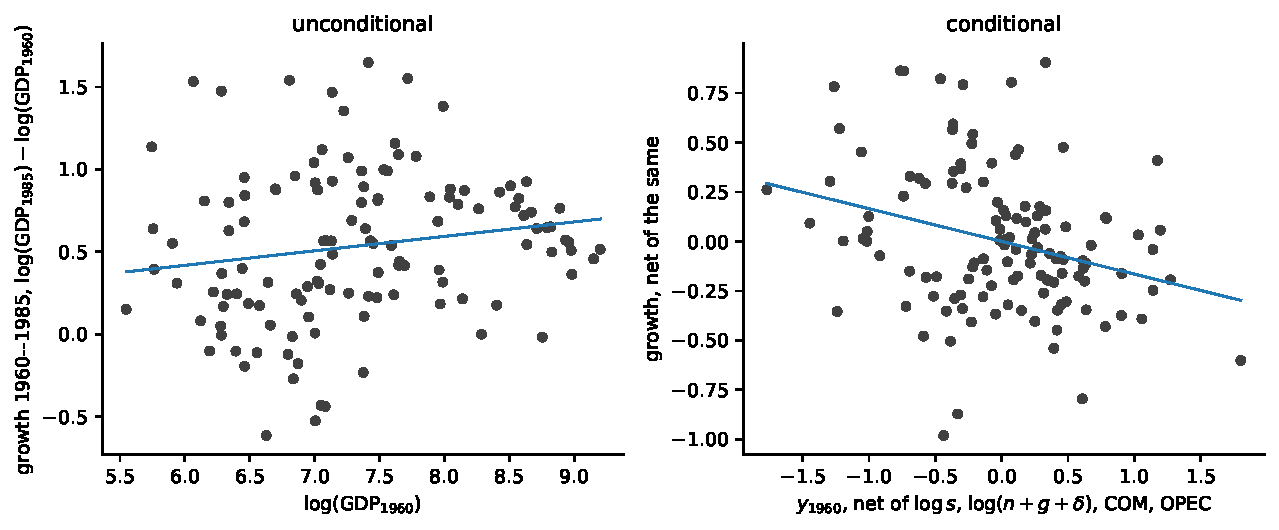
\includegraphics[width=0.98\textwidth]{figures/ch5_convergence.pdf}
\end{center}
\begin{center}
\begin{minipage}{0.82\textwidth}\small
Figure S5.1: cumulative growth 1960--1985 against log initial GDP per capita, 125 countries.
Left: raw (unconditional).  Right: both variables net of $\log s_i$, $\log(n_i+g+\delta)$, COM
and OPEC (the conditional relation estimated in equation $(2')$).
\end{minipage}
\end{center}

(b) \emph{Fixed-effects estimation.}  With $M=25$ equations ($m=1,\dots,25$;
$t_m=1960+m$), the within transformation sweeps out $\alpha_i$; the regressors are 24 year
dummies (1962--1985) and $y_{i,m-1}$, giving $\#\bs{\beta}=25$ coefficients estimated on a pooled
sample of $125\times25=3125$ transformed observations.  The estimate is
\[
\wh\rho_{\mathrm{FE}}=0.9380\quad(\text{SE } 0.0068),
\qquad
\wh\lambda=-\log(0.9380)=0.0640\ \text{per year}\quad(\text{SE } 0.0073),
\]
about $6.4\%$ per year, as the exercise anticipates --- nearly nine times the cross-section
estimate of part (a).  The standard errors use the \emph{correct} degrees of freedom
\bk{(5.2.17)}, $s^2=\SSR/(Mn-n-\#\bs{\beta})=11.8439/(3125-125-25)=0.003981$; the naive formula
\bk{(5.2.16)} gives $0.003821$ and standard errors smaller by the factor $0.980$ --- the text's
``very common mistake,'' small here only because $M=25$ is large.  The LSDV route (pooled OLS
with 125 country dummies and 24 year dummies) reproduces $\wh\rho$ and $\SSR$ to machine
precision ($2.9\times10^{-12}$), confirming Analytical Exercise 5.1.  Without the spherical
assumption, the robust standard error of Proposition 5.3 is $0.0089$ for $\wh\rho$ ($0.0095$ for
$\wh\lambda$), about 30\% larger than the spherical one --- mild evidence of conditional
heteroskedasticity or serial correlation in $\eta_{im}$.

As the exercise itself warns, consistency fails here: the system is dynamic, and by Analytical
Exercise 5.4 the fixed-effects estimator is inconsistent for $\rho$ (the cross orthogonalities
\bk{(5.2.6)} fail, $\E(y_{i,m-1}\eta_{ih})\neq0$ for $h\le m-1$; the Nickell bias is $O(1/M)$ and
downward, so the true $\rho$ is presumably even higher and $\lambda$ even larger).  The estimate
is reported purely ``to gain programming experience''; the contrast between $0.7\%$ in (a),
$6.4\%$ here and the next part is a vivid illustration of how much the answer depends on the
treatment of $\alpha_i$ and of dynamics.

(c) \emph{GMM on the first differences.}  Differencing the 25 equations gives $M-1=24$ equations,
\[
y_{i,m+1}-y_{im}=\xi'_m+(y_{im}-y_{i,m-1})\,\rho+(\eta_{i,m+1}-\eta_{im}),
\qquad m=1,\dots,24,
\]
with common $\rho$ and 24 free intercepts ($L=25$ coefficients), and instruments
$\mathbf{x}_{im}=(1,s_{i,m-1})'$ in equation $m$ --- for example $(1,s_{i,1960})$ in the first
equation.  This is the multiple-equation GMM of Section 4.6 with $48$ moment conditions; the
first step uses the 2SLS weighting (block-diagonal $\mathbf{S}_{\mathbf{xx}}^{-1}$), the second
step the efficient weight $\wh{\mathbf{S}}^{-1}$ estimated from the first-step residuals.  The
estimates are
\[
\wh\rho_{\text{2SLS}}=0.5859,
\qquad
\wh\rho_{\mathrm{GMM}}=0.6837\ \ (\text{SE } 0.0451),
\]
\[
\wh\lambda=-\log(0.6837)=0.380\ \text{per year}\quad(\text{SE } 0.066),
\]
i.e.\ about $38\%$ per year --- the exercise says ``about 36 percent per year!'', and the small
gap is accounted for by the efficient second-step weighting (the book's number comes from the
one-step estimator; our 2SLS first step gives $\lambda=53\%$, and the efficient GMM $38\%$, both
in the advertised ballpark of an order of magnitude beyond the cross-section estimate).
Sargan's statistic is $J=43.95$ on $\chi^2(23)$ ($p=0.005$), so the overidentifying restrictions
--- chiefly the assumption that the saving rate is orthogonal to the differenced error in every
equation --- are rejected at the 1\% level: either the saving rate is not exogenous for the
growth residual, or the common-$\rho$ restriction fails across periods.

Taken at face value, the three estimates of the speed of convergence tell one story: the
cross-section regression attributes to $\log s$ and $\log(n+g+\delta)$ much of what the panel
attributes to $\alpha_i$; removing the country effect raises $\lambda$ from under 1\% to 6.4\%;
and treating the lagged growth term as endogenous raises it further to about 36--38\%, a
half-life of two years.  Since the error in the growth regression is most plausibly a business
cycle, the last estimate --- which purges both the fixed effect and the simultaneity between
$\Delta y_{im}$ and $\Delta\eta_{im}$ --- is the one the model takes seriously, and it says
economies converge to their steady states very fast indeed.  The price, as the Sargan test shows,
is a set of instrument-validity assumptions the data are not entirely happy with.
\end{hee}


%% ========================================================================
\solchapter{6}{Serial Correlation}

\begin{center}
\begin{minipage}{0.86\textwidth}
\small
Solutions to all the exercises of Chapter 6 of Fumio Hayashi, \emph{Econometrics} (Princeton University
Press, 2000): the 35 review questions of Sections 6.1--6.8, the ten analytical exercises, and the two
empirical exercises (the Bekaert--Hodrick forward-exchange data and the Fama three-month T-bill
regression).  Propositions and equations cited as \bk{Proposition 6.8(b)} or \bk{(6.5.2)} refer to the
book.  The numerical parts are computed by \texttt{code/ch6.py}; the figures are in \texttt{figures/}.
\end{minipage}
\end{center}

\bigskip
\hrule
\bigskip

\solsection{6.1}{Modeling Serial Correlation: Linear Processes}

\begin{hrq}{6.1.1}{}
Let $S_n\equiv\sum_{j=0}^{n}|\gamma_j|$, a monotone nondecreasing sequence of real numbers.  By the Cauchy
criterion quoted in the question, $S_n$ converges to a (finite) real number if and only if it is Cauchy,
that is, $|S_m-S_n|\to0$ as $m,n\to\infty$.  For $m>n$,
\[
|S_m-S_n|=\sum_{j=n+1}^{m}|\gamma_j|,
\]
so the two statements are the same statement: $\{\gamma_j\}$ is absolutely summable
($\sum_{j=0}^{\infty}|\gamma_j|<\infty$, i.e.\ $S_n$ converges) if and only if the tail sums
$\sum_{j=n+1}^m|\gamma_j|$ vanish as $m,n\to\infty$.  The Cauchy form is often the usable one in proofs
because it does not mention the value of the limit: Analytical Exercise 6.2(a) uses exactly this, with
$a_n=\sum_{j=0}^n\psi_j^2$, to show that the MA($\infty$) partial sums form a mean-square Cauchy sequence.
\end{hrq}

\begin{hrq}{6.1.2}{}
Write $y_t=h_0x_t+h_1x_{t-1}$ and $y_{t-j}=h_0x_{t-j}+h_1x_{t-j-1}$ (means subtracted where necessary; the
calculation is unchanged).  Multiplying out and using covariance stationarity of $\{x_t\}$,
\[
\gamma_j^y=h_0^2\gamma_j^x+h_0h_1\gamma_{j+1}^x+h_1h_0\gamma_{j-1}^x+h_1^2\gamma_j^x
\]
because, for instance, $\Cov(x_t,x_{t-j-1})=\gamma_{j+1}^x$ (the two indices are $j+1$ apart) and
$\Cov(x_{t-1},x_{t-j})=\gamma_{j-1}^x$.  Collecting terms,
\[
\gamma_j^y=(h_0^2+h_1^2)\gamma_j^x+h_0h_1\bigl(\gamma_{j-1}^x+\gamma_{j+1}^x\bigr),
\]
which is the stated formula for all $j\ge1$; for $j=0$ it reads
$\gamma_0^y=(h_0^2+h_1^2)\gamma_0^x+h_0h_1(\gamma_{-1}^x+\gamma_1^x)
=(h_0^2+h_1^2)\gamma_0^x+2h_0h_1\gamma_1^x$ by the symmetry of scalar autocovariances, as claimed.
This is the special case $n=1$ of Analytical Exercise 6.3(a); the pattern --- a quadratic form in the
filter coefficients applied to a moving window of the input autocovariances --- is the general one.
\end{hrq}

\begin{hrq}{6.1.3}{}
All inverses exist because the leading coefficients are nonzero (\bk{(6.1.14)} and the sentences following
it).

($\Rightarrow$)  Suppose $\alpha(L)\beta(L)=\delta(L)$.  Multiply both sides from the left by
$\alpha(L)^{-1}$ and use associativity of filter multiplication (a direct consequence of the convolution
definition \bk{(6.1.12)}) together with the definition of the inverse, $\alpha(L)^{-1}\alpha(L)=1$
(\bk{(6.1.15a)}):
\[
\alpha(L)^{-1}\bigl[\alpha(L)\beta(L)\bigr]=\bigl[\alpha(L)^{-1}\alpha(L)\bigr]\beta(L)
=\beta(L)=\alpha(L)^{-1}\delta(L).
\]
($\Leftarrow$)  Suppose $\beta(L)=\alpha(L)^{-1}\delta(L)$.  Multiply from the left by $\alpha(L)$:
$\alpha(L)\beta(L)=\alpha(L)\alpha(L)^{-1}\delta(L)=\delta(L)$.

The second equivalence is identical with the roles reversed (multiply on the right by $\beta(L)^{-1}$ and
back).  The content is that the algebra of filters with nonzero leading coefficients is the algebra of
formal power series: one may ``multiply through'' by inverses exactly as with polynomials, and in the
\emph{scalar} case the order of the factors is irrelevant.
\rmk{Only the inverse operation is commutative in general; for matrix filters even that has to be proved
(Review Question 6.3.2), and ordinary multiplication is \emph{not} commutative (Review Question 6.3.3).}
\end{hrq}

\begin{hrq}{6.1.4}{}
The stability condition requires the roots of $\phi(z)=0$ to lie outside the unit circle, $|z|>1$.  By the
hint the two roots are $z=2(1\pm\sqrt{3}\,i)/3$; each has absolute value
\[
|z|=\frac{2}{3}\,|1\pm\sqrt{3}\,i|=\frac{2}{3}\sqrt{1+3}=\frac{4}{3}>1 .
\]
Both roots lie outside the unit circle, so the stability condition \emph{is} satisfied, and by
\bk{Proposition 6.3} the inverse filter $[1-\phi L-\phi^2L^2]^{-1}$ has coefficients bounded by a
geometrically declining sequence, hence absolutely summable.  The roots being complex means the
coefficients of the inverse oscillate (damped sine waves) as they decay: $|\psi_j|\le A(3/4)^j$ for some
$A$, with $3/4$ the reciprocal of the roots' modulus.
\end{hrq}

\begin{hrq}{6.1.5}{}
If $\lambda_1$ and $\lambda_2$ are the roots, $\phi(z)$ --- a quadratic with constant term $1$ --- factors
as
\[
\phi(z)=\Bigl(1-\frac{z}{\lambda_1}\Bigr)\Bigl(1-\frac{z}{\lambda_2}\Bigr)
=1-\Bigl(\frac{1}{\lambda_1}+\frac{1}{\lambda_2}\Bigr)z+\frac{1}{\lambda_1\lambda_2}z^2 .
\]
Equating coefficients with $1-\phi_1z-\phi_2z^2$ gives
$\phi_1=\lambda_1^{-1}+\lambda_2^{-1}$ and $\phi_2=-(\lambda_1\lambda_2)^{-1}$.  These are Vieta's
formulas for the \emph{reciprocal} roots; the same factorization is what makes the stability condition
``roots outside the unit circle'' equivalent to ``$|\lambda_k^{-1}|<1$'' in the companion-form analysis of
Analytical Exercise 6.7, where the $\lambda^{-1}$'s reappear as the eigenvalues of the matrix
$\mathbf{F}$.
\end{hrq}

\begin{hrq}{6.1.6}{}
Set $\alpha(L)=1-\phi L$ and $\beta(L)=\sum_{j\ge0}\phi^jL^j$, so $\beta_j=\phi^j$.  The convolution
$\delta_j=\sum_{k=0}^{j}\alpha_k\beta_{j-k}$ of \bk{(6.1.12)} gives
\[
\delta_0=\alpha_0\beta_0=1,\qquad
\delta_j=\alpha_0\beta_j+\alpha_1\beta_{j-1}=\phi^j-\phi\cdot\phi^{j-1}=0\quad(j\ge1),
\]
since only $\alpha_0$ and $\alpha_1$ are nonzero.  So $\delta(L)=1$, i.e.\
$(1-\phi L)\sum_{j\ge0}\phi^jL^j=1$: the geometric-series filter is the inverse of $1-\phi L$, exactly as
claimed in \bk{(6.1.20)}.  Note that nothing in this calculation requires $|\phi|<1$ --- the inverse exists
as a formal filter for any $\phi$ --- but $\{\phi^j\}$ is absolutely summable only when $|\phi|<1$, which is
the stationarity condition for AR(1): that is where, and only where, the inverse becomes usable on
covariance-stationary input processes (Propositions 6.2 and 6.3).
\end{hrq}

\solsection{6.2}{ARMA Processes}

\begin{hrq}{6.2.1}{}
\emph{Case $|\phi|<1$.}  By the MA($\infty$) representation \bk{(6.2.2)}, $y_{t-1}$ is a function of
$(\varepsilon_{t-1},\varepsilon_{t-2},\dots)$ and hence is uncorrelated with $\varepsilon_t$:
$\E(y_{t-1}\varepsilon_t)=0$ (the hint's statement).  Projecting $y_t=c+\phi y_{t-1}+\varepsilon_t$ on
$(1,y_{t-1})$,
\[
\wh{\E}^*(y_t\given 1,y_{t-1})=c+\phi y_{t-1}+\wh{\E}^*(\varepsilon_t\given 1,y_{t-1})=c+\phi y_{t-1},
\]
because $\varepsilon_t$ is orthogonal to $(1,y_{t-1})$ and so has zero projection.  The coefficients
$(c,\phi)$ do not depend on $t$ --- covariance stationarity makes the relevant second moments
time-invariant.

The projection need \emph{not} equal the conditional expectation: $\E(y_{t-1}\varepsilon_t)=0$ says
$\varepsilon_t$ is \emph{uncorrelated} with $y_{t-1}$, not \emph{mean-independent} of it.  If
$\{\varepsilon_t\}$ is merely white noise (not independent), $\E(\varepsilon_t\given y_{t-1})$ can be a
nonzero nonlinear function of $y_{t-1}$, and then $\E(y_t\given y_{t-1})\neq c+\phi y_{t-1}$.  With
independent white noise, the two do coincide.

On $(1,y_{t-1},y_{t-2})$ the projection is still $c+\phi y_{t-1}+0\cdot y_{t-2}$: $\varepsilon_t$ is
orthogonal to $y_{t-2}$ as well, and the coefficient on the extra regressor is zero.  The AR(1) structure
makes all lags beyond the first redundant for linear prediction.

\emph{Case $|\phi|>1$.}  Now the covariance-stationary solution \bk{(6.2.4)} expresses $y_t$ as a moving
average of \emph{future} innovations, $y_t-\mu=-\sum_{j=1}^{\infty}\phi^{-j}\varepsilon_{t+j}$.
Consequently $y_{t-1}$ is a function of $(\varepsilon_t,\varepsilon_{t+1},\dots)$ and
\[
\E\bigl[(y_{t-1}-\mu)\varepsilon_t\bigr]=-\phi^{-1}\sigma^2\neq0 ,
\]
so the hint's premise fails: $\E(y_{t-1}\varepsilon_t)\neq0$, and with it the argument that the projection
equals $c+\phi y_{t-1}$, because the projection of $\varepsilon_t$ on $(1,y_{t-1})$ is no longer zero.
The answer to the last question is \emph{no}: $\wh{\E}^*(y_t\given 1,y_{t-1})\neq c+\phi y_{t-1}$ when
$|\phi|>1$.  The autoregressive form of the equation is not the projection when the root is explosive ---
one more reason economic dynamics are written with $|\phi|<1$.
\end{hrq}

\begin{hrq}{6.2.2}{}
Successive substitution, as in the text's $\phi=1$ case, gives for any $j\ge1$
\[
y_t=(-1)^jy_{t-j}+\sum_{k=0}^{j-1}(-1)^k\varepsilon_{t-k},
\qquad\text{hence}\qquad
y_t-(-1)^jy_{t-j}=\sum_{k=0}^{j-1}(-1)^k\varepsilon_{t-k}.
\]
If $\{y_t\}$ were covariance-stationary, the variance of the left-hand side would be
$\Var(y_t)+\Var(y_{t-j})-2(-1)^j\Cov(y_t,y_{t-j})=2\gamma_0-2(-1)^j\gamma_j$, while the right-hand side
has variance $\sigma^2j$ by white noise.  So
\[
2\gamma_0-2(-1)^j\gamma_j=\sigma^2j .
\]
For $j$ even this reads $2(\gamma_0-\gamma_j)=\sigma^2j$, i.e.\
$\rho_j=1-\sigma^2j/(2\gamma_0)<-1$ for $j>4\gamma_0/\sigma^2$, contradicting $|\rho_j|\le1$.  Hence no
covariance-stationary solution exists.  (Intuitively, $\phi=-1$ makes the process flip sign
deterministically while accumulating variance: $y_t=(-1)^ty_0+\sum_{k=0}^{t-1}(-1)^k\varepsilon_{t-k}$,
whose variance grows linearly in $t$.)
\end{hrq}

\begin{hrq}{6.2.3}{}
(a) The stationarity condition \bk{(6.1.18)} requires every root $z$ of $\phi(z)=0$ to satisfy $|z|>1$.
Since $|1|=1$, $z=1$ is not a root, i.e.\ $\phi(1)=1-\phi_1-\dots-\phi_p\neq0$.  So the mean
$\mu=\phi(1)^{-1}c$ is well defined.

(b) Take expectations on both sides of the AR($p$) equation \bk{(6.2.6)},
$y_t=c+\phi_1y_{t-1}+\dots+\phi_py_{t-p}+\varepsilon_t$.  Covariance stationarity gives
$\E(y_{t-j})=\E(y_t)$ for every $j$, and white noise has mean zero, so
\[
\E(y_t)=c+(\phi_1+\dots+\phi_p)\E(y_t),
\qquad\text{i.e.}\qquad
\bigl[1-\phi_1-\dots-\phi_p\bigr]\E(y_t)=c .
\]
The bracket is $\phi(1)\neq0$ by part (a), so $\E(y_t)=c/\phi(1)=\phi(1)^{-1}c$, which is \bk{(6.2.8)}.
This confirms that the $\mu$ of the deviation-from-the-mean form \bk{(6.2.6$'$)} is indeed the mean; the
same argument applied to \bk{(6.2.9)} gives the mean of an ARMA($p,q$) process, $\mu=\phi(1)^{-1}c$ in
\bk{(6.2.11)}.
\end{hrq}

\begin{hrq}{6.2.4}{}
Apply the filter $\phi(L)$ to $y_t-\mu\equiv\phi(L)^{-1}\theta(L)\varepsilon_t$.  By the definition of the
inverse filter and its commutativity \bk{(6.1.15a)},
\[
\phi(L)(y_t-\mu)=\phi(L)\bigl[\phi(L)^{-1}\theta(L)\bigr]\varepsilon_t
=\bigl[\phi(L)\phi(L)^{-1}\bigr]\theta(L)\varepsilon_t=\theta(L)\varepsilon_t,
\]
which is exactly \bk{(6.2.9$'$)}.  The steps are legitimate because $\phi(L)^{-1}$ is absolutely summable
under the stationarity condition (\bk{Proposition 6.3}), so $\phi(L)^{-1}\theta(L)$ is an absolutely
summable filter (a convolution of absolutely summable sequences is absolutely summable) and
\bk{Proposition 6.2} makes both sides well-defined mean-square limits.  Combined with the uniqueness
argument used for AR(1) in the text (any covariance-stationary solution, when multiplied by
$\phi(L)^{-1}$, must equal this expression), this establishes \bk{Proposition 6.5(a)}.
\end{hrq}

\begin{hrq}{6.2.5}{}
The coefficients are determined by $\phi(L)\psi(L)=\theta(L)$, i.e.\ by the convolution formula
\bk{(6.1.12)} with $\alpha(L)=\phi(L)$, $\beta(L)=\psi(L)$ and $\delta(L)=\theta(L)$: for each $j\ge0$,
$\sum_{k=0}^{j}\alpha_k\psi_{j-k}=\theta_j$, where $\theta_j=0$ for $j>q$.

\emph{ARMA(3,1):} $\phi(L)=1-\phi_1L-\phi_2L^2-\phi_3L^3$, $\theta(L)=1+\theta_1L$:
\begin{align*}
L^0:&\ \psi_0=1,\\
L^1:&\ \psi_1-\phi_1\psi_0=\theta_1,\\
L^2:&\ \psi_2-\phi_1\psi_1-\phi_2\psi_0=0,\\
L^j:&\ \psi_j-\phi_1\psi_{j-1}-\phi_2\psi_{j-2}-\phi_3\psi_{j-3}=0,\quad j\ge3,
\end{align*}
since for $j\ge3$ all of $\phi$'s coefficients appear and the right-hand side is already zero (it vanishes
from $j\ge q+1=2$, but the $L^2$ equation still lacks the $\phi_3\psi_{-1}$ term only vacuously; the full
third-order recursion starts once both $j\ge p$ and $j\ge q+1$ hold).  Generally the homogeneous equation
\bk{(6.1.17)} governs $\psi_j$ from $j\ge\max(p,q+1)$; here $\max(3,2)=3$.

\emph{ARMA(1,2):} $\phi(L)=1-\phi_1L$, $\theta(L)=1+\theta_1L+\theta_2L^2$:
\[
\psi_0=1,\qquad \psi_1-\phi_1\psi_0=\theta_1,\qquad \psi_2-\phi_1\psi_1=\theta_2,\qquad
\psi_j-\phi_1\psi_{j-1}=0\ \ (j\ge3).
\]
The right-hand side is nonzero through $j=q=2$, so the homogeneous first-order recursion starts at
$j=\max(1,3)=3$ --- the book's answer, $j=3$.  The rule of thumb: the MA part delays the onset of the pure
AR recursion by its own order, because until lag $q$ the $\theta$'s keep entering the right-hand side.
\end{hrq}

\begin{hrq}{6.2.6}{}
By \bk{(6.2.20)}, $g_Y(z)=h(z)g_X(z)h(z^{-1})$.  Evaluating at $z=e^{-i\omega}$ (which lies on the unit
circle, so $z^{-1}=e^{i\omega}$) and dividing by $2\pi$,
\[
s_Y(\omega)=\frac{1}{2\pi}g_Y(e^{-i\omega})
=\frac{1}{2\pi}h(e^{-i\omega})\,g_X(e^{-i\omega})\,h(e^{i\omega})
=h(e^{-i\omega})\,s_X(\omega)\,h(e^{i\omega}) .
\]
Since $h(e^{-i\omega})h(e^{i\omega})=|h(e^{-i\omega})|^2$ (the coefficients of $h$ are real), this says
the spectrum of the output is the spectrum of the input multiplied by the squared modulus of the filter's
frequency response: $|h(e^{-i\omega})|^2$ is the \emph{gain}, showing exactly which frequencies the
filter amplifies or suppresses.  For the first-difference filter $1-L$, the gain is $2-2\cos\omega$, which
kills the zero-frequency component --- the spectral way of saying that differencing removes a unit root.
\end{hrq}

\begin{hrq}{6.2.7}{}
Substitute $z=e^{-i\omega}=\cos\omega-i\sin\omega$ into \bk{(6.2.14)}.  By the facts cited in the hint,
$z^j=[\cos\omega-i\sin\omega]^j=\cos(j\omega)-i\sin(j\omega)$ and $z^{-j}=\cos(j\omega)+i\sin(j\omega)$,
so $z^j+z^{-j}=2\cos(j\omega)$ and
\[
2\pi s_Y(\omega)=g_Y(e^{-i\omega})
=\gamma_0+\sum_{j=1}^{\infty}\gamma_j\bigl(z^j+z^{-j}\bigr)
=\gamma_0+2\sum_{j=1}^{\infty}\gamma_j\cos(j\omega),
\]
a sum of real terms ($\gamma_j$ is real for a real-valued process), absolutely convergent because
$\{\gamma_j\}$ is absolutely summable and $|\cos(j\omega)|\le1$.  Hence $s_Y(\omega)$ is real --- and in
fact nonnegative, though that requires a separate argument (the spectrum is the limit of the scaled
periodogram).  The oddness of sine is what makes the imaginary parts of $z^j$ and $z^{-j}$ cancel: a
covariance-stationary process has no ``direction'' in time at the level of second moments, so nothing
imaginary can survive.
\end{hrq}

\solsection{6.3}{Vector Processes}

\begin{hrq}{6.3.1}{}
With $\mathbf{y}_t-\bs{\mu}=\bs{\varepsilon}_t+\Theta_1\bs{\varepsilon}_{t-1}$ and
$\E(\bs{\varepsilon}_t\bs{\varepsilon}_{t-j}')=\Omega\,\indic{j=0}$ from \bk{(6.3.1)},
\begin{align*}
\Gamma_0&=\E\bigl[(\bs{\varepsilon}_t+\Theta_1\bs{\varepsilon}_{t-1})
(\bs{\varepsilon}_t+\Theta_1\bs{\varepsilon}_{t-1})'\bigr]
=\Omega+\Theta_1\Omega\Theta_1' ,\\
\Gamma_1&=\E\bigl[(\bs{\varepsilon}_t+\Theta_1\bs{\varepsilon}_{t-1})
(\bs{\varepsilon}_{t-1}+\Theta_1\bs{\varepsilon}_{t-2})'\bigr]
=\Theta_1\Omega ,
\end{align*}
because only the $\bs{\varepsilon}_{t-1}$ terms match; and $\Gamma_j=\mathbf{0}$ for $j\ge2$, with
$\Gamma_{-1}=\Gamma_1'=\Omega\Theta_1'$.  This is \bk{(6.3.4)},
$\Gamma_j=\sum_{k=j}^{\infty}\Psi_k\Omega\Psi_{k-j}'$, with $\Psi_0=\mathbf{I}$, $\Psi_1=\Theta_1$,
$\Psi_j=\mathbf{0}$ for $j\ge2$.  Note that $\Gamma_1$ need not be symmetric --- the order of the matrix
product matters, which is exactly why the transpose appears in $\Gamma_{-j}=\Gamma_j'$.
\end{hrq}

\begin{hrq}{6.3.2}{}
($\Rightarrow$)  Suppose $\mathbf{A}(L)\mathbf{B}(L)=\mathbf{I}$, i.e.\ by \bk{(6.3.5)},
$\mathbf{A}_0\mathbf{B}_0=\mathbf{I}$ and $\sum_{k=0}^{j}\mathbf{A}_k\mathbf{B}_{j-k}=\mathbf{0}$ for
$j\ge1$.  Let $\mathbf{C}(L)\equiv\mathbf{B}(L)\mathbf{A}(L)$; we show $\mathbf{C}(L)=\mathbf{I}$ by
identifying its coefficients recursively.  The constant term is
$\mathbf{C}_0=\mathbf{B}_0\mathbf{A}_0=\mathbf{A}_0^{-1}\mathbf{A}_0=\mathbf{I}$.  For $j=1$: from the
given, $\mathbf{A}_0\mathbf{B}_1=-\mathbf{A}_1\mathbf{B}_0$, so
$\mathbf{B}_1=-\mathbf{A}_0^{-1}\mathbf{A}_1\mathbf{B}_0$ and
\[
\mathbf{C}_1=\mathbf{B}_1\mathbf{A}_0+\mathbf{B}_0\mathbf{A}_1
=-\mathbf{A}_0^{-1}\mathbf{A}_1\mathbf{B}_0\mathbf{A}_0+\mathbf{B}_0\mathbf{A}_1
=-\mathbf{A}_0^{-1}\mathbf{A}_1+\mathbf{A}_0^{-1}\mathbf{A}_1=\mathbf{0},
\]
using $\mathbf{B}_0\mathbf{A}_0=\mathbf{I}\Rightarrow\mathbf{B}_0=\mathbf{A}_0^{-1}$, hence
$\mathbf{B}_0\mathbf{A}_1=\mathbf{A}_0^{-1}\mathbf{A}_1$ and
$\mathbf{A}_0^{-1}\mathbf{A}_1\mathbf{B}_0\mathbf{A}_0=\mathbf{A}_0^{-1}\mathbf{A}_1$.  The general step
is cleaner through a trick: $\mathbf{B}(L)\mathbf{A}(L)\mathbf{B}(L)=\mathbf{B}(L)
[\mathbf{A}(L)\mathbf{B}(L)]=\mathbf{B}(L)$, so $\mathbf{C}(L)\mathbf{B}(L)=\mathbf{B}(L)$; the filter
equation $\mathbf{C}(L)\mathbf{B}(L)=\mathbf{B}(L)$ determines the coefficients of $\mathbf{C}$
successively from
\[
\mathbf{C}_0\mathbf{B}_0=\mathbf{B}_0,\qquad
\sum_{k=0}^{j}\mathbf{C}_k\mathbf{B}_{j-k}=\mathbf{B}_j\ \ (j\ge1),
\]
each equation solvable because $\mathbf{B}_0$ is nonsingular.  The unique solution is
$\mathbf{C}_0=\mathbf{I}$, $\mathbf{C}_j=\mathbf{0}$ for $j\ge1$ (it satisfies the equations, and the
recursion admits only one solution).  Hence $\mathbf{B}(L)\mathbf{A}(L)=\mathbf{I}$.

($\Leftarrow$) is the same argument with the roles reversed.  So for square matrix filters with nonsingular
leading coefficients, a one-sided inverse is a two-sided inverse --- just as for finite-dimensional
matrices, and unlike the situation for general (e.g.\ one-sided shift) operators.
\end{hrq}

\begin{hrq}{6.3.3}{}
Take the first-degree filters $\mathbf{A}(L)=\mathbf{I}+\mathbf{A}_1L$,
$\mathbf{B}(L)=\mathbf{I}+\mathbf{B}_1L$ with
\[
\mathbf{A}_1=\begin{bmatrix}0&1\\0&0\end{bmatrix},\qquad
\mathbf{B}_1=\begin{bmatrix}0&0\\1&0\end{bmatrix}.
\]
The convolution \bk{(6.3.5)} gives the $L^2$ coefficient $\mathbf{A}_1\mathbf{B}_1$ for the product
$\mathbf{A}(L)\mathbf{B}(L)$ and $\mathbf{B}_1\mathbf{A}_1$ for $\mathbf{B}(L)\mathbf{A}(L)$:
\[
\mathbf{A}_1\mathbf{B}_1=\begin{bmatrix}1&0\\0&0\end{bmatrix}\neq
\begin{bmatrix}0&0\\0&1\end{bmatrix}=\mathbf{B}_1\mathbf{A}_1 .
\]
Hence
$\mathbf{A}(L)\mathbf{B}(L)=\mathbf{I}+(\mathbf{A}_1+\mathbf{B}_1)L+\mathbf{A}_1\mathbf{B}_1L^2
\neq\mathbf{B}(L)\mathbf{A}(L)$.  The moral: matrix filters can be manipulated exactly like scalar
filters \emph{except} that the order of multiplication must be preserved --- which is why \bk{(6.1.15b)}
needs separate statements for left- and right-multiplication in the matrix case (Review Question 6.3.4).
\end{hrq}

\begin{hrq}{6.3.4}{}
Both inverses exist because the leading matrices are nonsingular, and inverses commute (Review Question
6.3.2).

First equivalence.  ($\Rightarrow$)  Multiply $\mathbf{A}(L)\mathbf{B}(L)=\mathbf{D}(L)$ from the
\emph{left} by $\mathbf{A}(L)^{-1}$:
$\mathbf{A}(L)^{-1}\mathbf{A}(L)\mathbf{B}(L)=\mathbf{B}(L)=\mathbf{A}(L)^{-1}\mathbf{D}(L)$.
($\Leftarrow$)  Multiply from the left by $\mathbf{A}(L)$:
$\mathbf{A}(L)\mathbf{B}(L)=\mathbf{A}(L)\mathbf{A}(L)^{-1}\mathbf{D}(L)=\mathbf{D}(L)$.

Second equivalence.  ($\Rightarrow$)  Multiply from the \emph{right} by $\mathbf{B}(L)^{-1}$:
$\mathbf{A}(L)\mathbf{B}(L)\mathbf{B}(L)^{-1}=\mathbf{A}(L)=\mathbf{D}(L)\mathbf{B}(L)^{-1}$.
($\Leftarrow$)  Multiply from the right by $\mathbf{B}(L)$.

The only novelty relative to Review Question 6.1.3 is that the side on which one multiplies now matters:
to isolate $\mathbf{B}(L)$ one must multiply from the left, and to isolate $\mathbf{A}(L)$ from the
right.  Applied at the coefficient level this is the recursion used to build the MA($\infty$)
representation of a VAR, $\Psi(L)=\Phi(L)^{-1}$, one matrix at a time.
\end{hrq}

\begin{hrq}{6.3.5}{}
By definition, $\mathbf{A}(L)\mathbf{B}(L)\,[\mathbf{A}(L)\mathbf{B}(L)]^{-1}=\mathbf{I}$.  Consider the
candidate $\mathbf{C}(L)\equiv\mathbf{B}(L)^{-1}\mathbf{A}(L)^{-1}$:
\[
\mathbf{A}(L)\mathbf{B}(L)\mathbf{C}(L)
=\mathbf{A}(L)\,\mathbf{B}(L)\mathbf{B}(L)^{-1}\,\mathbf{A}(L)^{-1}
=\mathbf{A}(L)\mathbf{A}(L)^{-1}=\mathbf{I},
\]
using associativity and the definition of the two inverses.  By Review Question 6.3.2, a one-sided inverse
is the inverse, so $\mathbf{C}(L)=[\mathbf{A}(L)\mathbf{B}(L)]^{-1}$.  The order reverses, exactly as for
finite-dimensional matrices: to undo $\mathbf{A}$ then $\mathbf{B}$, undo $\mathbf{B}$ first.  The result
is used in the text's discussion of common roots in ARMA processes, where
$\psi(L)=[\alpha(L)\phi^*(L)]^{-1}\alpha(L)\theta^*(L)$ simplifies by cancellation only because the common
factor can be peeled off in the right order.
\end{hrq}

\solsection{6.4}{Estimating Autoregressions}

\begin{hrq}{6.4.1}{}
(a) By \bk{(6.4.2)}--\bk{(6.4.3)}, $\Avar(\hat\beta)=\sigma^2[\E(\mathbf{x}_t\mathbf{x}_t')]^{-1}$ with
$\mathbf{x}_t=(1,y_{t-1})'$, where
\[
\E(\mathbf{x}_t\mathbf{x}_t')=\begin{bmatrix}1&\mu\\ \mu&\mu^2+\gamma_0\end{bmatrix},
\qquad \mu=\frac{c}{1-\phi},\quad \gamma_0=\frac{\sigma^2}{1-\phi^2}.
\]
Inverting the $2\times2$ matrix (determinant $\gamma_0$), the $(2,2)$ element of the inverse is
$1/\gamma_0$.  Hence
\[
\Avar(\hat\phi)=\sigma^2\cdot\frac{1}{\gamma_0}=\sigma^2\cdot\frac{1-\phi^2}{\sigma^2}=1-\phi^2 .
\]
So $\sqrt{n}(\hat\phi-\phi)\convd \Norm(0,1-\phi^2)$: the closer $\phi$ is to one, the more precise the
estimator --- a preview of the nonstandard $|\phi|=1$ asymptotics of Chapter 9, where the rate changes
from $\sqrt{n}$ to $n$.

(b) Write $\mathbf{x}_t=(1,\wt{\mathbf{x}}_t')'$ with
$\wt{\mathbf{x}}_t=(y_{t-1},\dots,y_{t-p})'$.  Then, as in the hint,
\[
\E(\mathbf{x}_t\mathbf{x}_t')=
\begin{bmatrix}1 & \mu\mathbf{1}'\\ \mu\mathbf{1} & \mathbf{V}+\mu^2\mathbf{1}\mathbf{1}'\end{bmatrix},
\]
because $\E(\wt{\mathbf{x}}_t\wt{\mathbf{x}}_t')
=\Cov(\wt{\mathbf{x}}_t)+\E(\wt{\mathbf{x}}_t)\E(\wt{\mathbf{x}}_t)'=\mathbf{V}+\mu^2\mathbf{1}\mathbf{1}'$.
To verify the hint's inverse, multiply the matrix by the candidate
$\mathbf{A}=\bigl[\begin{smallmatrix}a&\mathbf{c}'\\ \mathbf{c}&\mathbf{V}^{-1}\end{smallmatrix}\bigr]$
with $a=1+\mu^2\mathbf{1}'\mathbf{V}^{-1}\mathbf{1}$ and $\mathbf{c}=-\mu\mathbf{V}^{-1}\mathbf{1}$:
\begin{align*}
(1,1):\quad& a+\mu\mathbf{1}'\mathbf{c}
=1+\mu^2\mathbf{1}'\mathbf{V}^{-1}\mathbf{1}-\mu^2\mathbf{1}'\mathbf{V}^{-1}\mathbf{1}=1,\\
(1,2):\quad& \mu a\mathbf{1}'+\mathbf{c}'(\mathbf{V}+\mu^2\mathbf{1}\mathbf{1}')
=\mu a\mathbf{1}'-\mu\mathbf{1}'-\mu^3(\mathbf{1}'\mathbf{V}^{-1}\mathbf{1})\mathbf{1}'
=\mu\bigl(a-1-\mu^2\mathbf{1}'\mathbf{V}^{-1}\mathbf{1}\bigr)\mathbf{1}'=\mathbf{0},\\
(2,2):\quad& \mu\mathbf{1}\mathbf{c}'+\mathbf{V}^{-1}(\mathbf{V}+\mu^2\mathbf{1}\mathbf{1}')
=-\mu^2\mathbf{1}(\mathbf{V}^{-1}\mathbf{1})'+\mathbf{I}+\mu^2\mathbf{V}^{-1}\mathbf{1}\mathbf{1}'
=\mathbf{I},
\end{align*}
the last because $\mathbf{1}(\mathbf{V}^{-1}\mathbf{1})'=(\mathbf{V}^{-1}\mathbf{1})\mathbf{1}'$ --- both
are the matrix with $(i,j)$ element $[\mathbf{V}^{-1}\mathbf{1}]_i$ (the vector $\mathbf{V}^{-1}\mathbf{1}$
is symmetric in this sense since $\mathbf{V}^{-1}$ is symmetric:
$\mathbf{1}'\mathbf{V}^{-1}=(\mathbf{V}^{-1}\mathbf{1})'$).  Hence the product is $\mathbf{I}$, confirming
\[
\bigl[\E(\mathbf{x}_t\mathbf{x}_t')\bigr]^{-1}
=\begin{bmatrix}a & \mathbf{c}'\\ \mathbf{c} & \mathbf{V}^{-1}\end{bmatrix}.
\]
The lower-right block gives
$\Avar(\hat{\bs{\phi}})=\sigma^2\mathbf{V}^{-1}$: the joint asymptotic variance of the autoregressive
coefficients is $\sigma^2$ times the inverse autocovariance matrix, independent of the mean $\mu$ --- the
sample analogue is the textbook formula
$\widehat{\Var}(\hat{\bs{\phi}})=s^2[\sum_t(\mathbf{y}_{t-1}-\bar{\mathbf{y}})
(\mathbf{y}_{t-1}-\bar{\mathbf{y}})']^{-1}$.  For $p=1$, $\mathbf{V}=\gamma_0$ and this reduces to part
(a).  As the hint notes, the display also shows $\E(\mathbf{x}_t\mathbf{x}_t')$ is nonsingular if and only
if $\mathbf{V}$ is, which is the rank condition \bk{Assumption 2.4} for the autoregression.
\end{hrq}

\begin{hrq}{6.4.2}{}
Equation $m$ of the system is $y_{tm}=\mathbf{x}_t'\bs{\delta}_m+\varepsilon_{tm}$ with
$\mathbf{x}_t=\mathbf{y}_{t-1}$ and $\bs{\delta}_m$ the $m$-th \emph{row} of $\mathbf{A}$, transposed.
Equation-by-equation OLS gives
\[
\hat{\bs{\delta}}_m=\Bigl(\sum_{t=2}^n\mathbf{y}_{t-1}\mathbf{y}_{t-1}'\Bigr)^{-1}
\sum_{t=2}^n\mathbf{y}_{t-1}y_{tm},
\]
so the $m$-th row of $\widehat{\mathbf{A}}$ is
$\hat{\bs{\delta}}_m'=\bigl(\sum_ty_{tm}\mathbf{y}_{t-1}'\bigr)
\bigl(\sum_t\mathbf{y}_{t-1}\mathbf{y}_{t-1}'\bigr)^{-1}$.  Stacking the $M$ rows,
\[
\widehat{\mathbf{A}}=\Bigl(\sum_{t=2}^n\mathbf{y}_t\mathbf{y}_{t-1}'\Bigr)
\Bigl(\sum_{t=2}^n\mathbf{y}_{t-1}\mathbf{y}_{t-1}'\Bigr)^{-1},
\]
as claimed.  This is the matrix analogue of the univariate AR(1) slope
$\hat\phi=\sum_ty_ty_{t-1}/\sum_ty_{t-1}^2$: since every equation has the same regressors, the estimates
stack, and $\widehat{\mathbf{A}}$ is what a package returns for a VAR(1) with no constant.  Note the order
of the two factors --- the cross-moment matrix multiplies the inverse second-moment matrix on the
\emph{right}, the transpose of the scalar case, because the rows of $\mathbf{A}$ multiply
$\mathbf{y}_{t-1}$ from the left.
\end{hrq}

\solsection{6.5}{Asymptotics for Sample Means of Serially Correlated Processes}

\begin{hrq}{6.5.1}{}
Write $\mathbf{y}\equiv(y_t,\dots,y_{t-n+1})'$ and let $\mathbf{V}_n\equiv\Var(\mathbf{y})$ be the
$n\times n$ autocovariance matrix (the same for any block of $n$ consecutive dates, by covariance
stationarity).  Since $\sqrt{n}\,\bar y_n=\frac{1}{\sqrt{n}}\mathbf{1}'\mathbf{y}$,
\[
\Var(\sqrt{n}\,\bar y_n)=\frac1n\,\mathbf{1}'\Var(\mathbf{y})\,\mathbf{1}
=\frac1n\mathbf{1}'\mathbf{V}_n\mathbf{1}
=\frac1n\sum_{t=1}^n\sum_{s=1}^n\gamma_{|t-s|}
=\gamma_0+2\sum_{j=1}^{n-1}\Bigl(1-\frac{j}{n}\Bigr)\gamma_j ,
\]
the last equality by counting, for each lag $j$, the $n-j$ pairs $(t,s)$ with $|t-s|=j$ in each direction
--- which is \bk{(6.5.2)}.  The quadratic-form version is useful because it makes the long-run variance a
property of the whole autocovariance matrix: the sample mean ``sees'' every autocovariance, with weights
tapering linearly from $1$ to $0$ as the lag grows.
\end{hrq}

\begin{hrq}{6.5.2}{}
By \bk{(6.2.19)} with $g_\varepsilon(z)=\sigma^2$, the autocovariance-generating function of
$y_t=\mu+\psi(L)\varepsilon_t$ is $g_Y(z)=\sigma^2\psi(z)\psi(z^{-1})$.  The long-run variance is
$g_Y(1)$ (see \bk{(6.2.15)} and the text after \bk{Proposition 6.8}), so
\[
\Avar(\bar y)=\sum_{j=-\infty}^{\infty}\gamma_j=g_Y(1)=\sigma^2\psi(1)^2
=\sigma^2\Bigl(\sum_{j=0}^{\infty}\psi_j\Bigr)^2,
\]
since $\psi(1)=\sum_j\psi_j$ converges by absolute summability.  One check: for MA(1),
$\psi(1)=1+\theta_1$ and $\gamma_0+2\gamma_1=\sigma^2[(1+\theta_1^2)+2\theta_1]
=\sigma^2(1+\theta_1)^2$.  Notice the long-run variance is zero if $\psi(1)=0$: the shocks cancel ``in
the long run'' and $\bar y$ converges faster than $1/\sqrt n$ (compare Review Question 6.5.5).
\end{hrq}

\begin{hrq}{6.5.3}{}
\emph{Consistency: yes, without independence.}  $\{\gamma_j\}$ vanishes geometrically,
$\gamma_j=\phi^j\gamma_0$, so $\gamma_j\to0$ and \bk{Proposition 6.8(a)} gives $\bar y\convms\mu$, hence
$\bar y\convp\mu=c/(1-\phi)$.

\emph{Asymptotic variance.}  With independent white noise the CLT \bk{Proposition 6.9} applies, since the
MA($\infty$) coefficients $\psi_j=\phi^j$ are absolutely summable.  Two computations of the limit:

(i) \emph{Summing the autocovariances.}
\[
\Avar(\bar y)=\gamma_0+2\sum_{j=1}^{\infty}\gamma_j
=\gamma_0\Bigl(1+2\sum_{j=1}^{\infty}\phi^j\Bigr)
=\gamma_0\Bigl(1+\frac{2\phi}{1-\phi}\Bigr)
=\frac{1+\phi}{1-\phi}\,\gamma_0
=\frac{1+\phi}{1-\phi}\cdot\frac{\sigma^2}{1-\phi^2}
=\frac{\sigma^2}{(1-\phi)^2},
\]
which is the book's answer $[(1+\phi)/(1-\phi)]\gamma_0$.

(ii) \emph{From the filter.}  $\psi(1)=\sum_j\phi^j=1/(1-\phi)$, so by Review Question 6.5.2,
$\Avar(\bar y)=\sigma^2/(1-\phi)^2$ --- the same number, as it must be.

So $\sqrt{n}(\bar y-\mu)\convd \Norm\bigl(0,\sigma^2/(1-\phi)^2\bigr)$.  The factor
$(1+\phi)/(1-\phi)$ measures how much serial correlation inflates the variance of the sample mean: it
diverges as $\phi\uparrow1$ --- again foreshadowing the unit-root asymptotics of Chapter 9 --- and is less
than one for negative $\phi$.
\end{hrq}

\begin{hrq}{6.5.4}{}
By \bk{(6.3.13)}, $\mathbf{G}_Y(z)=\mathbf{H}(z)\mathbf{G}_X(z)\mathbf{H}(z^{-1})'$, and by \bk{(6.5.6)}
the long-run covariance matrix is $\mathbf{G}_Y(1)$.  Evaluating at $z=1$,
\[
\sum_{j=-\infty}^{\infty}\Gamma_j^y=\mathbf{G}_Y(1)
=\mathbf{H}(1)\,\mathbf{G}_X(1)\,\mathbf{H}(1)'
=\mathbf{H}(1)\Bigl(\sum_{j=-\infty}^{\infty}\Gamma_j^x\Bigr)\mathbf{H}(1)',
\]
since $\mathbf{H}(z^{-1})$ at $z=1$ is $\mathbf{H}(1)$.  For the one-term filter,
$\mathbf{H}(1)=\mathbf{H}_0+\mathbf{H}_1$.  This is the matrix version of ``long-run variance of output
$=$ [filter at $1$] $\times$ long-run variance of input $\times$ [filter at $1$]$'$'', and it is exactly
the formula behind VARHAC: with $\mathbf{g}_t$ modeled as a VAR, the implied long-run variance of
$\mathbf{g}_t$ is $[\mathbf{I}-\sum_j\widehat{\mathbf{A}}_j]^{-1}\widehat{\Omega}
[\mathbf{I}-\sum_j\widehat{\mathbf{A}}_j]'^{-1}$, which is \bk{(6.6.15)}.
\end{hrq}

\begin{hrq}{6.5.5}{}
The autocovariances are $\gamma_0=2\sigma^2$, $\gamma_1=-\sigma^2$, $\gamma_j=0$ for $j\ge2$, so
\[
\sum_{j=-\infty}^{\infty}\gamma_j=2\sigma^2+2(-\sigma^2)=0 .
\]
Equivalently, $\psi(L)=1-L$ has $\psi(1)=0$, and the long-run variance is $\sigma^2\psi(1)^2=0$.  The
MA(1) with $\theta=-1$ is the ``unit-root MA'': it is the first difference of white noise, so its partial
sums telescope,
$\sum_{t=1}^ny_t=\varepsilon_n-\varepsilon_0$, and
$\Var(\sqrt n\,\bar y_n)=\Var(\varepsilon_n-\varepsilon_0)/n=2\sigma^2/n\to0$: the sample mean converges
at a rate faster than $1/\sqrt n$.  A singular (here, zero) long-run variance is exactly the case excluded
by the nonsingularity clause of \bk{Assumption 3.5$'$} --- GMM asymptotics need the long-run variance to
be positive definite.
\rmk{The example is the boundary between stationary and unit-root behaviour: $y_t=(1-L)\varepsilon_t$ is
stationary but ``overdifferenced'' --- it is the difference of a series that did not need differencing.
Chapter 9's tests for unit roots amount to testing whether the MA polynomial has a root at $1$.}
\end{hrq}

\solsection{6.6}{Incorporating Serial Correlation in GMM}

\begin{hrq}{6.6.1}{}
It is the OLS estimator.  With $\mathbf{x}_t=\mathbf{z}_t$, the model is exactly identified ($K=L$), so
GMM sets the sample orthogonality conditions to zero:
$\bar{\mathbf{g}}(\bs{\delta})=\frac1n\sum_t\mathbf{z}_t(y_t-\mathbf{z}_t'\bs{\delta})=\mathbf{0}$, whose
solution is $\hat{\bs{\delta}}=(\mathbf{Z}'\mathbf{Z})^{-1}\mathbf{Z}'\mathbf{y}$ regardless of the
weighting matrix --- every GMM estimator, hence the efficient one, is OLS.  What serial correlation changes
is not the point estimate but the standard errors: the consistent estimator of the asymptotic variance is
\bk{(3.5.2)} with $\widehat{\mathbf{S}}$ a HAC estimator of the long-run variance \bk{(6.6.1)}, e.g.\ the
truncated or Bartlett kernel sums of $\widehat{\Gamma}_j$.  So the recipe ``estimate by OLS, but compute
Newey--West standard errors'' \emph{is} efficient GMM in the just-identified case --- there is no
efficiency gain available from GLS-type corrections when the regressors are merely predetermined (Section
6.7 makes this precise).
\end{hrq}

\begin{hrq}{6.6.2}{}
\emph{Consistent: yes.}  Consistency of GMM requires only the orthogonality conditions
$\E(\mathbf{g}_t)=\mathbf{0}$ (\bk{Assumption 3.3}), ergodic stationarity and identification; the
probability limit of $\hat{\bs{\delta}}(\widehat{\mathbf{W}})$ is $\bs{\delta}$ whatever the autocovariance
structure of $\{\mathbf{g}_t\}$, because the argument
``$\bar{\mathbf{g}}(\hat{\bs{\delta}})\convp\mathbf{0}$ forces $\hat{\bs{\delta}}\convp\bs{\delta}$'' never
uses the absence of serial correlation.  Serial correlation is a property of the \emph{dynamics} of the
moment conditions, not of their means.

\emph{Efficient: no.}  Efficiency requires $\plim\widehat{\mathbf{W}}=\mathbf{S}^{-1}$ with $\mathbf{S}$
the long-run variance \bk{(6.6.1)}.  An estimator built on the presumption of no serial correlation uses
$\mathbf{S}=\E(\mathbf{g}_t\mathbf{g}_t')=\Gamma_0$, omitting $\sum_{j\neq0}\Gamma_j$, and so is the
efficient GMM estimator of a different (wrongly specified) weighting scheme.  Two consequences: its
asymptotic variance exceeds that of the truly efficient estimator (unless the omitted autocovariances
happen to sum to zero), and --- equally important in practice --- the standard errors it reports, computed
from $\Gamma_0$ alone, are inconsistent, so the associated $t$ and Wald tests have the wrong size even
though the point estimates are fine.  In the just-identified case ($\mathbf{x}_t=\mathbf{z}_t$) the point
estimate is numerically identical to the efficient one (OLS), and only the standard errors are wrong ---
which is why the ``HAC correction'' is often described as fixing the standard errors of OLS.
\end{hrq}

\solsection{6.7}{Estimation under Conditional Homoskedasticity (Optional)}

\begin{hrq}{6.7.1}{}
With $n=3$ and autocovariances vanishing after lag $q=1$, \bk{(6.7.6)}--\bk{(6.7.7)} give
\[
\widehat{\Omega}=\begin{bmatrix}\hat\omega_0 & \hat\omega_1 & 0\\
\hat\omega_1 & \hat\omega_0 & \hat\omega_1\\ 0 & \hat\omega_1 & \hat\omega_0\end{bmatrix},
\qquad \hat\omega_j=\frac1n\sum_{t=j+1}^n\hat\varepsilon_t\hat\varepsilon_{t-j}.
\]
The $(k,\ell)$ element of $\mathbf{X}'\widehat{\Omega}\,\mathbf{X}$ is
$\sum_{t=1}^3\sum_{s=1}^3 x_{tk}\widehat{\Omega}_{ts}x_{s\ell}$.  The diagonal terms ($t=s$) contribute
$\hat\omega_0\sum_tx_{tk}x_{t\ell}$; the off-diagonal terms contribute
$\hat\omega_1\sum_{|t-s|=1}x_{tk}x_{s\ell}
=\hat\omega_1\sum_{t=2}^3(x_{tk}x_{t-1,\ell}+x_{t-1,k}x_{t\ell})$.  Dividing by $n$,
\[
\frac1n\mathbf{X}'\widehat{\Omega}\,\mathbf{X}
=\widehat{\Gamma}_0+\widehat{\Gamma}_1+\widehat{\Gamma}_1',
\qquad
\widehat{\Gamma}_j\equiv\hat\omega_j\,\frac1n\sum_{t=j+1}^n\mathbf{x}_t\mathbf{x}_{t-j}'
\ \ \text{as in \bk{(6.7.4)}},
\]
which is \bk{(6.6.4)} with $q=1$.  That is exactly \bk{(6.7.5)}.  The general case is the same
computation: the band structure of $\widehat{\Omega}$ (zeros beyond the $q$-th diagonal, or kernel
weights on the diagonals) collects the products $x_{tk}x_{s\ell}$ into the weighted autocovariances of
$\{\mathbf{x}_t\hat\varepsilon_t\}$ that the kernel estimator sums.
\end{hrq}

\begin{hrq}{6.7.2}{}
Under conditional homoskedasticity with serial correlation, \bk{(6.7.3)} gives
$\Gamma_j=\omega_j\E(\mathbf{x}_t\mathbf{x}_{t-j}')$, and \bk{(6.7.5)} writes the estimated long-run
variance as $\widehat{\mathbf{S}}=\frac1n\mathbf{X}'\widehat{\Omega}\,\mathbf{X}$.  Sargan's statistic
generalizes as Hansen's $J$ evaluated at the efficient GMM estimator under conditional homoskedasticity
\bk{(6.7.9)}: with $\bar{\mathbf{g}}=\frac1n\mathbf{X}'(\mathbf{y}-\mathbf{Z}\hat{\bs{\delta}})$ the sample
orthogonality conditions,
\[
J=n\,\bar{\mathbf{g}}'\widehat{\mathbf{S}}^{-1}\bar{\mathbf{g}}
=\bigl[\mathbf{X}'(\mathbf{y}-\mathbf{Z}\hat{\bs{\delta}})\bigr]'
\bigl[\mathbf{X}'\widehat{\Omega}\,\mathbf{X}\bigr]^{-1}
\bigl[\mathbf{X}'(\mathbf{y}-\mathbf{Z}\hat{\bs{\delta}})\bigr]
\ \convd\ \chi^2(K-L),
\]
under the null that all $K$ orthogonality conditions hold --- exactly as in \bk{(3.8.10$'$)}, the only
change being that $\widehat{\mathbf{S}}$ (equivalently $\widehat{\Omega}$) now reflects serial
correlation, through the truncated or Bartlett weights in \bk{(6.7.7)}--\bk{(6.7.8)}, instead of being
proportional to $\mathbf{X}'\mathbf{X}$.  When $\widehat{\Omega}=\hat\sigma^2\mathbf{I}_n$ (no serial
correlation) the display collapses to \bk{(3.8.10$'$)}, since then
$J=\frac{1}{\hat\sigma^2}(\mathbf{y}-\mathbf{Z}\hat{\bs{\delta}})'\mathbf{P}_X
(\mathbf{y}-\mathbf{Z}\hat{\bs{\delta}})$ with $\mathbf{P}_X=\mathbf{X}(\mathbf{X}'\mathbf{X})^{-1}
\mathbf{X}'$ --- Sargan's original statistic, the explained sum of squares from regressing the 2SLS
residuals on all the instruments, divided by $\hat\sigma^2$.
\end{hrq}

\begin{hrq}{6.7.3}{}
No.  Write the efficient estimator under conditional homoskedasticity,
\[
\hat{\bs{\delta}}=\bigl[\mathbf{Z}'\mathbf{X}(\mathbf{X}'\widehat{\Omega}\,\mathbf{X})^{-1}
\mathbf{X}'\mathbf{Z}\bigr]^{-1}\mathbf{Z}'\mathbf{X}
(\mathbf{X}'\widehat{\Omega}\,\mathbf{X})^{-1}\mathbf{X}'\mathbf{y}.
\]
This is a GLS-flavored instrumental-variables estimator: the instruments enter through the ``effective
regressor matrix''
$\widetilde{\mathbf{Z}}\equiv\mathbf{X}(\mathbf{X}'\widehat{\Omega}\mathbf{X})^{-1}\mathbf{X}'\mathbf{Z}$,
and $\hat{\bs{\delta}}=(\widetilde{\mathbf{Z}}'\mathbf{Z})^{-1}\widetilde{\mathbf{Z}}'\mathbf{y}$.
Without serial correlation ($\widehat{\Omega}\propto\mathbf{I}_n$),
$\widetilde{\mathbf{Z}}=\mathbf{P}_X\mathbf{Z}$ and, when the columns of $\mathbf{Z}$ are among those of
$\mathbf{X}$, $\mathbf{P}_X\mathbf{Z}=\mathbf{Z}$, so $\hat{\bs{\delta}}$ collapses to OLS --- the Section
3.8 result.  With serial correlation the weighting matrix
$(\mathbf{X}'\widehat{\Omega}\mathbf{X})^{-1}$ is not proportional to $(\mathbf{X}'\mathbf{X})^{-1}$, the
projection identity fails, and the estimator is a genuine GMM estimator distinct from OLS, even though
every regressor is a valid instrument.  The intuition: with serial correlation the efficient linear
combination of the orthogonality conditions is not the one that sets
$\mathbf{Z}'(\mathbf{y}-\mathbf{Z}\bs{\delta})=\mathbf{0}$; the efficient combination downweights the
moment conditions in a way that reflects the error autocovariances.
\end{hrq}

\begin{hrq}{6.7.4}{}
Without conditional homoskedasticity the $(t,s)$ element of $\widehat{\Omega}$ must reproduce the product
of the residuals $\hat\varepsilon_t\hat\varepsilon_s$ itself, with the kernel weight attached, because
$\Gamma_j=\E(\mathbf{g}_t\mathbf{g}_{t-j}')$ no longer factors as $\omega_j\E(\mathbf{x}_t
\mathbf{x}_{t-j}')$.  Following the hint, set
\[
\widehat{\Omega}_{ts}=\hat\varepsilon_t\hat\varepsilon_s\;k\Bigl(\frac{|t-s|}{q(n)+1}\Bigr):
\]
for the truncated kernel at known $q$, $\widehat{\Omega}_{ts}=\hat\varepsilon_t\hat\varepsilon_s$ for
$|t-s|\le q$ and $0$ beyond; for the Bartlett kernel,
\[
\widehat{\Omega}_{ts}=\Bigl(1-\frac{|t-s|}{q(n)+1}\Bigr)\hat\varepsilon_t\hat\varepsilon_s
\qquad \bigl(|t-s|\le q(n)\bigr),
\]
and zero beyond.  Indeed, the $(k,\ell)$ element of $\frac1n\mathbf{X}'\widehat{\Omega}\mathbf{X}$ is then
\[
\frac1n\sum_{t}\sum_{s}x_{tk}x_{s\ell}\widehat{\Omega}_{ts}
=\sum_{j=-q(n)}^{q(n)}k\Bigl(\frac{|j|}{q(n)+1}\Bigr)\,
\frac1n\sum_{t=|j|+1}^{n}x_{tk}\hat\varepsilon_t\,x_{t-|j|,\ell}\hat\varepsilon_{t-|j|},
\]
which is the $(k,\ell)$ element of
$\widehat{\Gamma}_0+\sum_{j\ge1}k(\cdot)(\widehat{\Gamma}_j+\widehat{\Gamma}_j')$ with
$\widehat{\Gamma}_j=\frac1n\sum_t\mathbf{g}_t\mathbf{g}_{t-j}'$ --- the kernel estimator \bk{(6.6.3)}.
So the same data-matrix formula \bk{(6.7.5)} covers both cases; the difference is only whether the
autocovariances of the errors and of the instruments can be estimated separately (they can, under
conditional homoskedasticity, via \bk{(6.7.4)} --- which is statistically cheaper) or must be estimated
jointly through the products $\mathbf{x}_t\hat\varepsilon_t$.
\end{hrq}

\begin{hrq}{6.7.5}{}
\emph{OLS.}  $\sqrt n(\hat\beta_{\mathrm{OLS}}-\beta)=\bigl(\frac1n\sum_tz_t^2\bigr)^{-1}
\frac{1}{\sqrt n}\sum_tz_t\varepsilon_t$.  The AR(1) error has autocovariances
$\omega_j=\phi^{|j|}\sigma_\varepsilon^2$, so by \bk{(6.7.3)} in scalar form, the autocovariances of the
moment process $\{z_t\varepsilon_t\}$ are
$\Gamma_j=\omega_j\E(z_tz_{t-j})=\phi^{|j|}\sigma_\varepsilon^2\rho_{|j|}\sigma_z^2$, and its long-run
variance is
\[
S=\sigma_\varepsilon^2\sigma_z^2\Bigl[1+2\sum_{j=1}^{\infty}\phi^j\rho_j\Bigr],
\qquad
\Avar(\hat\beta_{\mathrm{OLS}})=\frac{S}{(\sigma_z^2)^2}
=\frac{\sigma_\varepsilon^2}{\sigma_z^2}\Bigl[1+2\sum_{j=1}^{\infty}\phi^j\rho_j\Bigr].
\]

\emph{GLS.}  With known $\phi$, GLS is OLS on the quasi-differenced equation
$y_t-\phi y_{t-1}=\beta(z_t-\phi z_{t-1})+\eta_t$, i.e.\
\[
\hat\beta_{\mathrm{GLS}}-\beta
=\frac{\frac1n\sum_t\tilde z_t\eta_t}{\frac1n\sum_t\tilde z_t^2},
\qquad \tilde z_t\equiv z_t-\phi z_{t-1}.
\]
Because $\{\eta_t\}$ is independent with $\E(\tilde z_t\eta_t)=0$ by assumption,
$\{\tilde z_t\eta_t\}$ is a martingale difference sequence, so its long-run variance is
$\E(\tilde z_t^2\eta_t^2)=\sigma_\eta^2\E(\tilde z_t^2)$ (conditional homoskedasticity), where
\[
\E(\tilde z_t^2)=\sigma_z^2\bigl(1+\phi^2-2\phi\rho_1\bigr).
\]
Therefore
\[
\Avar(\hat\beta_{\mathrm{GLS}})
=\frac{\sigma_\eta^2\,\E(\tilde z_t^2)}{[\E(\tilde z_t^2)]^2}
=\frac{\sigma_\eta^2}{\sigma_z^2\bigl(1+\phi^2-2\phi\rho_1\bigr)}
=\frac{(1-\phi^2)\,\sigma_\varepsilon^2}{\sigma_z^2(1+\phi^2-2\phi\rho_1)},
\]
using $\sigma_\eta^2=(1-\phi^2)\sigma_\varepsilon^2$.  Note that the GLS variance depends on
$\{\rho_j\}$ only through $\rho_1$: GLS exploits the AR(1) structure of the error exactly.

\emph{A configuration with $\Avar_{\mathrm{OLS}}<\Avar_{\mathrm{GLS}}$.}  Take $\phi=0.9$ and
$\rho_1=0.99$, $\rho_j=0$ for $j\ge2$.  Then
\[
\Avar_{\mathrm{OLS}}=\frac{\sigma_\varepsilon^2}{\sigma_z^2}\bigl(1+2\times0.9\times0.99\bigr)
=2.782\,\frac{\sigma_\varepsilon^2}{\sigma_z^2},
\qquad
\Avar_{\mathrm{GLS}}=\frac{0.19}{1.81-1.782}\,\frac{\sigma_\varepsilon^2}{\sigma_z^2}
=6.79\,\frac{\sigma_\varepsilon^2}{\sigma_z^2},
\]
so OLS is more than twice as precise as GLS.  What happens: with $\rho_1$ close to $\phi$ and both close
to one, the quasi-differenced regressor $\tilde z_t=z_t-\phi z_{t-1}$ nearly vanishes
($\E\tilde z_t^2=0.028\,\sigma_z^2$), destroying the identifying variation GLS uses, while the
untransformed regression keeps the full variation of $z_t$.

\emph{Why this is consistent with GMM efficiency.}  The efficient GMM ranking of Section 6.6 is a ranking
of estimators that exploit \emph{the same} orthogonality conditions $\E(z_t\varepsilon_t)=0$; among those,
OLS is efficient in this just-identified model (Review Question 6.6.1).  GLS is not in that class: its
normal equations involve $\tilde z_t\eta_t=(z_t-\phi z_{t-1})\eta_t$, i.e.\ they exploit the
\emph{different} moment conditions $\E(z_t\eta_t)=0$ and $\E(z_{t-1}\eta_t)=0$ --- conditions that are
about the white-noise innovation, not about $\varepsilon_t$, and that the model's assumption
$\E(z_t\varepsilon_t)=0$ for predetermined $z_t$ does not deliver (predeterminedness gives
$\E(z_{t-j}\varepsilon_t)=0$ only for $j$ of the appropriate sign; $\E(z_{t-1}\eta_t)=0$ is an extra
assumption, which happens to be imposed here).  Even granting those extra moments, GLS is superior only
when the AR(1) model for the error is exactly right \emph{and} the regressor dynamics cooperate; the
example shows the failure of the second caveat.  Hence the chapter's practical message: with predetermined
regressors, keep the OLS point estimate and fix the standard errors; do not quasi-difference.
\end{hrq}

\solsection{6.8}{Application: Forward Exchange Rates as Optimal Predictors}

\begin{hrq}{6.8.1}{}
In the regression $\varepsilon_t=\mu+u_t$ with the single regressor $\mathbf{x}_t=1$, the OLS estimate of
$\mu$ is $\hat\mu=\bar\varepsilon$, and the moment process is
$\mathbf{g}_t=\mathbf{x}_t\hat u_t=\hat u_t=\varepsilon_t-\bar\varepsilon$.  The estimated
autocovariances of $\mathbf{g}_t$ are
\[
\hat\Gamma_j=\frac1n\sum_{t=j+1}^{n}\hat u_t\hat u_{t-j}=\hat\gamma_j,
\]
the sample autocovariances of the demeaned forecast error --- the $1\times1$ version of \bk{(6.6.2)}.
With $\mathbf{S}_{\mathbf{xx}}=1$, the HAC asymptotic variance is
$\widehat{\Avar(\hat\mu)}=\widehat{\mathbf{S}}$ with
\[
\widehat{\mathbf{S}}=\hat\gamma_0+2\sum_{j=1}^{4}\hat\gamma_j ,
\]
the $q=4$ truncated kernel estimator.  The standard error of $\hat\mu=\bar\varepsilon$ is
$\sqrt{\widehat{\mathbf{S}}/n}$, and the $t$-ratio for $\mu=0$ is
\[
t=\frac{\bar\varepsilon}{\sqrt{\widehat{\mathbf{S}}/n}}
=\frac{\sqrt n\,\bar\varepsilon}{\sqrt{\hat\gamma_0+2\sum_{j=1}^4\hat\gamma_j}},
\]
which is \bk{(6.8.7)}.  So the unconditional test \emph{is} a GMM test with one instrument (the constant)
and the truncated HAC estimator at four lags.  Numerically (\texttt{code/ch6.py}), the three currencies
give $t=-0.35$ (yen), $0.65$ (DM) and $0.43$ (pound) --- Table 6.1's non-rejection of market efficiency
at the unconditional level.
\end{hrq}

\begin{hrq}{6.8.2}{}
\emph{Random walk.}  Market efficiency with risk neutrality, \bk{(6.8.3)}, requires
$f_t=\E(s_{t+2}\given I_t)$.  For a random walk (with or without drift), $\E(s_{t+2}\given I_t)=s_t$
(plus twice the drift), so $f_t=s_t$: the forward premium $f_t-s_t$ is identically zero, the regressor in
\bk{(6.8.9)} has no variance, and $\E(\mathbf{x}_t\mathbf{x}_t')$ for $\mathbf{x}_t=(1,f_t-s_t)'$ is
singular --- the \emph{identification condition} \bk{Assumption 3.4} fails.  The orthogonality condition
still holds --- $\varepsilon_t$ is a two-period forecast error, orthogonal to $I_t$ --- but with a
constant regressor there is nothing to estimate; the equation reduces to $\varepsilon_t=\beta_0+u_t$.  As
the book's answer states: the violated assumption is identification.

\emph{Stationary AR(1).}  Iterating the AR(1) forward,
\[
s_{t+2}=c+\phi s_{t+1}+\eta_{t+2}=c+\phi(c+\phi s_t+\eta_{t+1})+\eta_{t+2}
=(1+\phi)c+\phi^2s_t+\eta_{t+2}+\phi\eta_{t+1}.
\]
Taking $\E(\cdot\given I_t)$ kills the $\eta$'s (they are i.i.d.\ with mean zero, dated after $t$), so
\[
f_t=\E(s_{t+2}\given I_t)=(1+\phi)c+\phi^2s_t ,
\]
as claimed; and subtracting,
$\varepsilon_t=s_{t+2}-f_t=\eta_{t+2}+\phi\eta_{t+1}$, an MA(1) with parameter $\phi$ --- serial
correlation up to lag $1$, the two-week analogue of the four-week overlap in the data.  Note that
identification is restored: $f_t-s_t=(1+\phi)c-(1-\phi^2)s_t$ varies with $s_t$, so the forward premium
moves and the regression \bk{(6.8.9)} has a nondegenerate regressor.  Random-walk spot rates destroy the
test not by making the orthogonality conditions fail but by making the instrument useless.
\end{hrq}

\begin{hrq}{6.8.3}{}
The information set $I_t$ (Friday of week $t$) includes the current spot and forward rates, hence
$f_t-s_t$ and $\mathbf{x}_t$; and because $\varepsilon_{t-j}=s30_{t-j}-f_{t-j}$ is observed once the
delivery date of week $t-j$'s contract has passed --- which is after the Friday of week $t-j+4$ --- $I_t$
also includes $\varepsilon_{t-5},\varepsilon_{t-6},\dots$, hence $\mathbf{g}_{t-5},\mathbf{g}_{t-6},\dots$
(their other ingredient, $\mathbf{x}_{t-j}$, is in $I_t$ for $j\ge1$).  So both $\mathbf{x}_t$ and the
conditioning variables are functions of $I_t$.  By the law of iterated expectations,
\[
\E(\mathbf{g}_t\given \mathbf{g}_{t-5},\mathbf{g}_{t-6},\dots)
=\E\bigl[\E(\mathbf{x}_t\varepsilon_t\given I_t)\given \mathbf{g}_{t-5},\dots\bigr]
=\E\bigl[\mathbf{x}_t\,\E(\varepsilon_t\given I_t)\given \mathbf{g}_{t-5},\dots\bigr]
=\mathbf{0},
\]
because $\E(\varepsilon_t\given I_t)=0$ is the market efficiency hypothesis \bk{(6.8.3)}.  This is
\bk{(6.8.10)}: the moment process inherits the ``martingale difference at displacement 5'' property of
the forecast error, so its autocovariances vanish beyond lag 4, $\Gamma_j=\mathbf{0}$ for $j\ge5$, and
$\mathbf{S}$ is consistently estimated by the truncated sum \bk{(6.6.4)} with $q=4$ --- the basis of
Table 6.2.
\end{hrq}

\problemset{6}{Problem Set for Chapter 6: Analytical Exercises}

\begin{hax}{6.1}{}
(a) Define the mean-square norm $\|x\|\equiv\sqrt{\E(x^2)}$ and expand along the hint:
\[
z-z'=(z-z_n)+(z_n-z'),\qquad
\|z-z'\|^2=\|z-z_n\|^2+2\E\bigl[(z-z_n)(z_n-z')\bigr]+\|z_n-z'\|^2 .
\]
By the Cauchy--Schwarz inequality for expectations, $|\E(xy)|\le\|x\|\,\|y\|$, the middle term is bounded
by $2\|z-z_n\|\,\|z_n-z'\|$, so
\[
\|z-z'\|^2\le\bigl(\|z-z_n\|+\|z_n-z'\|\bigr)^2,
\qquad\text{i.e.}\qquad
\|z-z'\|\le\|z-z_n\|+\|z_n-z'\|
\]
--- the triangle inequality for $\|\cdot\|$.  Both terms on the right converge to zero by hypothesis, so
$\|z-z'\|=0$, that is, $\E[(z-z')^2]=0$.

(b) By Chebychev's inequality, for every $\varepsilon>0$,
\[
\Prob\bigl(|z-z'|>\varepsilon\bigr)\le\frac{\E[(z-z')^2]}{\varepsilon^2}=0,
\]
so $\Prob(|z-z'|>\varepsilon)=0$ for every $\varepsilon>0$.  The event
$\{z\neq z'\}=\bigcup_{k=1}^{\infty}\{|z-z'|>1/k\}$ is a countable union of zero-probability events, hence
has probability zero: $\Prob(z=z')=1$.

So a mean-square limit, when it exists, is unique up to a zero-probability event --- which is what makes
the definition of the infinite sum \bk{(6.1.3)} as ``the'' mean square limit of the partial sums
unambiguous.  Mean square convergence is convergence in the Hilbert space $L^2$ of square-integrable
random variables; this exercise proves that $L^2$ limits are unique a.s., the first fact every $L^2$
construction (conditional expectations included) needs.
\end{hax}

\begin{hax}{6.2}{}
Let $y_{t,n}\equiv\mu+\sum_{j=0}^{n}\psi_j\varepsilon_{t-j}$, the partial sum.

(a) For $m>n$, by white noise ($\E(\varepsilon_s\varepsilon_u)=\sigma^2\indic{s=u}$),
\[
\E\bigl[(y_{t,m}-y_{t,n})^2\bigr]
=\E\Bigl[\Bigl(\sum_{j=n+1}^{m}\psi_j\varepsilon_{t-j}\Bigr)^2\Bigr]
=\sigma^2\sum_{j=n+1}^{m}\psi_j^2 .
\]
Absolute summability of $\{\psi_j\}$ implies square summability: $|\psi_j|\to0$, so $|\psi_j|\le1$
eventually, hence $\psi_j^2\le|\psi_j|$ eventually and $\sum_j\psi_j^2$ converges by comparison.  A
convergent series has vanishing tails (Review Question 6.1.1), so $\sum_{j=n+1}^m\psi_j^2\to0$ as
$m,n\to\infty$.  By fact (i), $\{y_{t,n}\}$ converges in mean square; the limit is $y_t$ by definition.
No property of $t$ was used, so the limit exists for every $t$.

(b) $y_{t,n}\convms y_t$ by (a), so fact (ii) with $x_n=y_{t,n}$ gives
\[
\E(y_t)=\lim_{n\to\infty}\E(y_{t,n})=\lim_{n\to\infty}\Bigl(\mu+\sum_{j=0}^n\psi_j\E(\varepsilon_{t-j})
\Bigr)=\mu .
\]

(c) Fix $j\ge0$.  Since $y_{t,n}\convms y_t$ and $y_{t-j,n}\convms y_{t-j}$, fact (ii) with
$x_n=y_{t,n}-\mu$, $z_n=y_{t-j,n}-\mu$ gives
\[
\gamma_j\equiv\E[(y_t-\mu)(y_{t-j}-\mu)]
=\lim_{n\to\infty}\E\Bigl[\sum_{k=0}^{n}\psi_k\varepsilon_{t-k}
\sum_{\ell=0}^{n}\psi_\ell\varepsilon_{t-j-\ell}\Bigr]
=\sigma^2\sum_{\ell=0}^{\infty}\psi_{\ell+j}\psi_\ell ,
\]
where the second equality uses white noise (only terms with $t-k=t-j-\ell$, i.e.\ $k=\ell+j$, survive)
and the last the convergence of the partial sums (the full double sum is dominated by
$(\sum_k|\psi_k|)^2<\infty$).  This is \bk{(6.1.7)}.  The result depends on $t$ only through the lag $j$,
and the mean is constant by (b); hence $\{y_t\}$ is covariance-stationary.

(d) The goal is $\sum_{j=0}^{\infty}|\gamma_j|<\infty$ (the full sum over $j\in\mathbb{Z}$ then follows
by symmetry $\gamma_{-j}=\gamma_j$).  From (c), for $j\ge0$,
\[
|\gamma_j|\le\sigma^2\sum_{k=0}^{\infty}|\psi_{j+k}|\,|\psi_k|,
\]
and summing over $j$ and interchanging the order of summation (legitimate for nonnegative summands ---
Tonelli's theorem, the content of the book's facts (i)--(ii) for this case),
\begin{align*}
\sum_{j=0}^{\infty}|\gamma_j|
&\le\sigma^2\sum_{j=0}^{\infty}\sum_{k=0}^{\infty}|\psi_{j+k}\psi_k|
=\sigma^2\sum_{k=0}^{\infty}|\psi_k|\sum_{j=0}^{\infty}|\psi_{j+k}|\\
&\le\sigma^2\Bigl(\sum_{k=0}^{\infty}|\psi_k|\Bigr)\Bigl(\sum_{i=0}^{\infty}|\psi_i|\Bigr)
=\sigma^2\Bigl(\sum_{k=0}^{\infty}|\psi_k|\Bigr)^2<\infty ,
\end{align*}
because $\sum_{j\ge0}|\psi_{j+k}|\le\sum_i|\psi_i|$ for every $k$.  Hence $\{\gamma_j\}$ is absolutely
summable: absolutely summable coefficients produce absolutely summable autocovariances.
\rmk{The bound $\sum_j|\gamma_j|\le\sigma^2(\sum_j|\psi_j|)^2$ is the cleanest statement of the chapter's
central theme: summability properties pass from the filter to the autocovariances.  The long-run variance
itself is the square \emph{without} the absolute values, $\sigma^2\psi(1)^2$ (Review Question 6.5.2) ---
which can be much smaller than the bound, and can vanish.}
\end{hax}

\begin{hax}{6.3}{}
(a) Write everything as deviations from means, $y_{t,n}-\E y_{t,n}=\sum_k h_k(x_{t-k}-\mu_x)$, and expand:
\[
\Cov(y_{t,n},y_{t-j,n})
=\E\Bigl[\sum_{k=0}^nh_k(x_{t-k}-\mu_x)\sum_{\ell=0}^nh_\ell(x_{t-j-\ell}-\mu_x)\Bigr]
=\sum_{k=0}^n\sum_{\ell=0}^nh_kh_\ell\,\gamma_{(t-k)-(t-j-\ell)}^x ,
\]
and the lag is $(t-j-\ell)-(t-k)=k-\ell-j$, so by the symmetry $\gamma_{-m}^x=\gamma_m^x$ the term
indexed $(k,\ell)$ is $\gamma_{j+\ell-k}^x=\gamma_{|j+k-\ell|}$ with the roles of $k$ and $\ell$ swapped
--- the displayed double sum.

For $n=1$ this is Review Question 6.1.2.  If $\{x_t\}$ is white noise with variance $\sigma^2$,
$\gamma_m^x=\sigma^2\indic{m=0}$, so only pairs with $k=\ell+j$ survive:
\[
\gamma_j^{(n)}=\sigma^2\!\!\sum_{\substack{0\le\ell\le n\\0\le\ell+j\le n}}\!\!h_{\ell+j}h_\ell
=\sigma^2\sum_{\ell=0}^{n-j}h_{\ell+j}h_\ell\quad(0\le j\le n),
\]
which is \bk{(6.1.2)} for the MA($n$) process with $\theta_\ell=h_\ell$ --- and for $j>n$ the sum is
empty, $\gamma_j=0$: an MA($n$) has exactly $n$ nonzero autocovariances.

(b) By \bk{Proposition 6.2(a)}, $y_{t,n}\convms y_t$ and $y_{t-j,n}\convms y_{t-j}$.  Fact (ii) of
Analytical Exercise 6.2 then gives
$\gamma_j^y=\lim_n\gamma_j^{(n)}=\lim_n\sum_{k,\ell\le n}h_kh_\ell\gamma_{j+k-\ell}^x$.  The double
series converges absolutely, because
\[
\sum_{k,\ell}|h_kh_\ell|\,|\gamma_{j+k-\ell}^x|
\le\gamma_0^x\Bigl(\sum_k|h_k|\Bigr)^2<\infty
\]
($|\gamma_m^x|\le\gamma_0^x$ for every $m$), so the limit of the truncated sums equals the full double
sum:
\[
\gamma_j^y=\sum_{k=0}^{\infty}\sum_{\ell=0}^{\infty}h_kh_\ell\,\gamma_{j+k-\ell}^x .
\]
This is the promised generalization of \bk{(6.1.7)}: filtering convolves the filter with itself and
applies the result to the input's autocovariance sequence.  In the frequency domain the same statement is
the single line $s_Y(\omega)=|h(e^{-i\omega})|^2s_X(\omega)$ of Review Question 6.2.6 --- one reason the
spectral approach is popular: double convolutions become multiplications.
\end{hax}

\begin{hax}{6.4}{}
(a) Substitute $y_j=c_{10}\lambda_1^j+c_{20}\lambda_2^j$ into the right-hand side:
\[
\phi_1y_{j-1}+\phi_2y_{j-2}
=\sum_{k=1}^{2}c_{k0}\lambda_k^{j-2}\bigl(\phi_1\lambda_k+\phi_2\bigr).
\]
Each $\lambda_k$ solves $\lambda^2=\phi_1\lambda+\phi_2$ (the associated polynomial equation
\bk{(6.1.18$'$)} for $p=2$), so $\phi_1\lambda_k+\phi_2=\lambda_k^2$ and the sum becomes
$\sum_kc_{k0}\lambda_k^j=y_j$: the display solves the difference equation for any $(c_{10},c_{20})$.
The initial conditions pin down the constants: at $j=0$ and $j=1$,
\[
c_{10}+c_{20}=y_0,\qquad c_{10}\lambda_1+c_{20}\lambda_2=y_1,
\]
a $2\times2$ linear system with determinant $\lambda_2-\lambda_1\neq0$ (distinct roots), solved by
\[
c_{10}=\frac{y_1-\lambda_2y_0}{\lambda_1-\lambda_2},\qquad
c_{20}=\frac{\lambda_1y_0-y_1}{\lambda_1-\lambda_2}.
\]

(b) Here $\phi_1=4/3$, $\phi_2=-4/9$, and the single root $\lambda=2/3$ satisfies both
$\lambda^2=\phi_1\lambda+\phi_2$ and $2\lambda=\phi_1$ (a double root also solves the derivative of the
polynomial: $\lambda^2-\phi_1\lambda-\phi_2=(\lambda-2/3)^2$).  For $y_j=(c_{10}+c_{11}j)\lambda^j$,
\[
\phi_1y_{j-1}+\phi_2y_{j-2}
=\lambda^{j-2}\bigl[\phi_1\lambda\bigl(c_{10}+c_{11}(j-1)\bigr)+\phi_2\bigl(c_{10}+c_{11}(j-2)\bigr)\bigr].
\]
The coefficient of $c_{10}$ is $\phi_1\lambda+\phi_2=\lambda^2$; the coefficient of $c_{11}$ is
\[
\phi_1\lambda(j-1)+\phi_2(j-2)=j(\phi_1\lambda+\phi_2)-(\phi_1\lambda+2\phi_2)
=j\lambda^2-(\phi_1\lambda+2\phi_2),
\]
and $\phi_1\lambda+2\phi_2=\frac43\cdot\frac23-2\cdot\frac49=0$.  So the bracket equals
$\lambda^2(c_{10}+c_{11}j)$ and the whole expression is $(c_{10}+c_{11}j)\lambda^j=y_j$, as required.
The extra solution $j\lambda^j$ is the hallmark of a repeated root.

(c) Pick any $b\in(\delta,1)$ and set $u_j\equiv j^m(\delta/b)^j$.  With $r\equiv\delta/b<1$,
$u_{j+1}/u_j=(1+1/j)^mr\to r<1$ as $j\to\infty$, so by the ratio test $\sum_ju_j$ converges, and a
fortiori $u_j\to0$.  A convergent sequence is bounded: there is $A>0$ with $u_j\le A$ for all $j$, that
is, $j^m\delta^j\le Ab^j$.  (The point: exponentials dominate powers, so any geometric decay slightly
slower than $\delta^j$ still swallows the polynomial factor $j^m$.)

(d) By the representation (5) in the book, $y_j=\sum_{k=1}^{K}\sum_{m=0}^{r_k-1}c_{km}j^m\lambda_k^j$.
Hence, with $c\equiv\max_{k,m}|c_{km}|$,
\[
|y_j|\le c\sum_{k=1}^{K}\sum_{m=0}^{r_k-1}j^m|\lambda_k|^j .
\]
The stability condition gives $|\lambda_k|<1$ for every $k$.  Apply part (c) with $\delta=|\lambda_k|$
and exponent $m$: there exist $A_{km}>0$ and $b_{km}\in(|\lambda_k|,1)$ with
$j^m|\lambda_k|^j\le A_{km}b_{km}^j$.  Set $A^*\equiv\max_{k,m}A_{km}$ and $b\equiv\max_{k,m}b_{km}<1$;
then $j^m|\lambda_k|^j\le A^*b^j$ for every $(k,m)$, and summing the $p$ terms (recall
$\sum_kr_k=p$),
\[
|y_j|\le c\,p\,A^*\,b^j\equiv Ab^j,\qquad A\equiv cpA^*,\quad 0<b<1 .
\]
So every solution of a stable $p$-th order homogeneous difference equation is bounded by a geometrically
declining sequence --- the result used in the text (\bk{(6.1.19)}) to prove that inverses of stable lag
polynomials have absolutely summable coefficients, since $\sum_jAb^j=A/(1-b)<\infty$.
\end{hax}

\begin{hax}{6.5}{}
(a) For $j\ge1$, multiply $y_t-\mu=\phi(y_{t-1}-\mu)+\varepsilon_t$ by $y_{t-j}-\mu$ and take
expectations:
\[
\gamma_j=\phi\gamma_{j-1}+\E\bigl[(y_{t-j}-\mu)\varepsilon_t\bigr].
\]

(b) By the MA($\infty$) representation \bk{(6.2.2)},
$y_{t-1}-\mu=\sum_{k=0}^{\infty}\phi^k\varepsilon_{t-1-k}$ is a function of
$(\varepsilon_{t-1},\varepsilon_{t-2},\dots)$, while white noise gives
$\E(\varepsilon_{t-1-k}\varepsilon_t)=0$ for every $k\ge0$.  Hence
$\E[(y_{t-1}-\mu)\varepsilon_t]=0$; and since $\E(\varepsilon_t)=0$,
$\E(y_{t-1}\varepsilon_t)=\E[(y_{t-1}-\mu)\varepsilon_t]+\mu\E(\varepsilon_t)=0$.  The same argument with
$t-j$ in place of $t-1$ gives $\E[(y_{t-j}-\mu)\varepsilon_t]=0$ for every $j\ge1$.

(c) Part (b) kills the second term in (a), giving the recursion.  For $j=0$, multiply the equation by
$y_t-\mu$ itself:
\[
\gamma_0=\E[(y_t-\mu)^2]=\phi\,\E[(y_t-\mu)(y_{t-1}-\mu)]+\E[(y_t-\mu)\varepsilon_t].
\]
The first term is $\phi\gamma_1$ (by definition of $\gamma_1$); for the second, substitute the equation
once more and use (b):
$\E[(y_t-\mu)\varepsilon_t]=\phi\E[(y_{t-1}-\mu)\varepsilon_t]+\E(\varepsilon_t^2)=\sigma^2$.
Together:
\[
\gamma_0=\phi\gamma_1+\sigma^2,\qquad \gamma_j=\phi\gamma_{j-1}\ \ (j\ge1)
\]
--- the Yule--Walker equations for AR(1).

(d) From the $j=1$ equation, $\gamma_1=\phi\gamma_0$; substituting into the first equation,
$\gamma_0=\phi^2\gamma_0+\sigma^2$, so
\[
\gamma_0=\frac{\sigma^2}{1-\phi^2},\qquad
\gamma_j=\phi^j\gamma_0=\frac{\phi^j\sigma^2}{1-\phi^2}\ \ (j\ge0),
\]
matching \bk{(6.2.5)} from the MA route.  The two methods are complementary: the MA representation makes
the answers immediate once $\{\psi_j\}$ is known, while Yule--Walker obtains the autocovariances directly
from the difference equation --- and generalizes to AR($p$) as a $p$-term recursion in $\gamma_j$,
solvable by exactly the apparatus of Analytical Exercise 6.4.
\end{hax}

\begin{hax}{6.6}{}
(a) Iterate the deviation form $x_t=\phi x_{t-1}+\varepsilon_t$:
\[
x_t=\phi(\phi x_{t-2}+\varepsilon_{t-1})+\varepsilon_t
=\phi^2x_{t-2}+\phi\varepsilon_{t-1}+\varepsilon_t=\dots
=\sum_{j=0}^{n}\phi^j\varepsilon_{t-j}+\phi^{n+1}x_{t-n-1},
\]
after $n+1$ substitutions.  So $x_t-x_{t,n}=\phi^{n+1}x_{t-n-1}$ with
$x_{t,n}\equiv\sum_{j=0}^n\phi^j\varepsilon_{t-j}$.

(b) Compute the mean square distance:
\[
\E\bigl[(x_{t,n}-x_t)^2\bigr]=\E\bigl[\phi^{2(n+1)}x_{t-n-1}^2\bigr]
=\phi^{2(n+1)}\gamma_0 ,
\]
because covariance stationarity makes $\E(x_{t-n-1}^2)=\Var(y_{t-n-1})=\gamma_0$, a constant not
depending on $n$.  Since $|\phi|<1$, $\phi^{2(n+1)}\gamma_0\to0$: $x_{t,n}\convms x_t$.

(c) By Analytical Exercise 6.2(a) (applied with $\psi_j=\phi^j$, absolutely summable since $|\phi|<1$),
the partial sums $x_{t,n}$ converge in mean square to the infinite sum
$\sum_{j=0}^{\infty}\phi^j\varepsilon_{t-j}$ --- that infinite sum is \emph{defined} as the mean square
limit.  By (b) the same sequence converges in mean square to $x_t$.  Mean square limits are unique up to
a zero-probability event (Analytical Exercise 6.1), so
\[
x_t=\sum_{j=0}^{\infty}\phi^j\varepsilon_{t-j}
\quad\text{a.s.},\qquad\text{i.e.}\qquad
y_t=\mu+\sum_{j=0}^{\infty}\phi^j\varepsilon_{t-j},
\]
which is \bk{(6.2.2)}.  The point of doing this without filters: the only inputs are the geometric decay
of the remainder $\phi^{n+1}x_{t-n-1}$ and the boundedness of the variance --- covariance stationarity of
the solution plus $|\phi|<1$ \emph{forces} the MA($\infty$) representation.  Analytical Exercise 6.7
repeats the argument for AR($p$) with the companion matrix $\mathbf{F}^n$ playing the role of $\phi^n$.
\end{hax}

\begin{hax}{6.7}{}
(a) The first row of $\bs{\xi}_t=\mathbf{F}\bs{\xi}_{t-1}+\mathbf{v}_t$ is the AR($p$) equation
\bk{(6.2.6$'$)}; the remaining rows are the identities $y_{t-j}=y_{t-j}$.  Iterating exactly as in
Analytical Exercise 6.6(a),
\[
\bs{\xi}_t=\mathbf{F}\bs{\xi}_{t-1}+\mathbf{v}_t
=\mathbf{F}^2\bs{\xi}_{t-2}+\mathbf{F}\mathbf{v}_{t-1}+\mathbf{v}_t=\dots
=\sum_{j=0}^{n}\mathbf{F}^j\mathbf{v}_{t-j}+\mathbf{F}^{n+1}\bs{\xi}_{t-n-1}.
\]

(b) For $p=2$,
\[
\lambda\mathbf{I}-\mathbf{F}=\begin{bmatrix}\lambda-\phi_1 & -\phi_2\\ -1 & \lambda\end{bmatrix},
\qquad
|\lambda\mathbf{I}-\mathbf{F}|=(\lambda-\phi_1)\lambda-\phi_2=\lambda^2-\phi_1\lambda-\phi_2 ,
\]
the associated polynomial equation \bk{(6.1.18$'$)} for $p=2$: the eigenvalues of the companion matrix are
the reciprocals of the roots of $\phi(z)=0$ (Review Question 6.1.5).

(c) $\mathbf{F}^3=\mathbf{F}\mathbf{F}\mathbf{F}
=(\mathbf{T}\Lambda\mathbf{T}^{-1})(\mathbf{T}\Lambda\mathbf{T}^{-1})(\mathbf{T}\Lambda\mathbf{T}^{-1})
=\mathbf{T}\Lambda(\mathbf{T}^{-1}\mathbf{T})\Lambda(\mathbf{T}^{-1}\mathbf{T})\Lambda\mathbf{T}^{-1}
=\mathbf{T}\Lambda^3\mathbf{T}^{-1}$.  The same computation for general $n$ is the induction
$\mathbf{F}^{n+1}=\mathbf{F}^n\mathbf{F}
=\mathbf{T}\Lambda^n\mathbf{T}^{-1}\mathbf{T}\Lambda\mathbf{T}^{-1}
=\mathbf{T}\Lambda^{n+1}\mathbf{T}^{-1}$.

(d) From (a), $\bs{\xi}_t-\bs{\xi}_{t,n}=\mathbf{F}^{n+1}\bs{\xi}_{t-n-1}$.  Mean square convergence is
elementwise, so it suffices that every element of $\mathbf{F}^{n+1}\bs{\xi}_{t-n-1}$ converge in mean
square to zero.  By (c), each element of $\mathbf{F}^n$ is a linear combination (with fixed coefficients
from $\mathbf{T}$ and $\mathbf{T}^{-1}$) of $\lambda_1^n,\dots,\lambda_p^n$; the stationarity condition
says $|\lambda_k|<1$ for all $k$, so by Analytical Exercise 6.4(d) each element of $\mathbf{F}^n$ is
bounded in absolute value by $Ab^n$ for some $A>0$ and $0<b<1$.  Covariance stationarity gives
$\E(\xi_{t-n-1,\ell}^2)=\gamma_0<\infty$ for every component, so the $k$-th element satisfies, by
Cauchy--Schwarz,
\[
\E\Bigl[\Bigl(\sum_{\ell=1}^{p}[\mathbf{F}^{n+1}]_{k\ell}\,\xi_{t-n-1,\ell}\Bigr)^{\!2}\Bigr]
\le p\,\gamma_0\sum_{\ell=1}^{p}[\mathbf{F}^{n+1}]_{k\ell}^2
\le p^2\gamma_0A^2b^{2(n+1)}\longrightarrow 0 .
\]
Hence $\bs{\xi}_{t,n}\convms\bs{\xi}_t$.

(e) The partial sums $\bs{\xi}_{t,n}$ converge in mean square both to $\bs{\xi}_t$ (by (d)) and to
$\sum_{j=0}^{\infty}\mathbf{F}^j\mathbf{v}_{t-j}$ (the definition of that infinite sum, which exists
elementwise by the same geometric bound and Analytical Exercise 6.2(a) applied componentwise).  Uniqueness
of mean square limits (Analytical Exercise 6.1) gives
\[
\bs{\xi}_t=\sum_{j=0}^{\infty}\mathbf{F}^j\mathbf{v}_{t-j}\quad\text{a.s.}
\]
The first row of this vector equation is the MA($\infty$) representation of $y_t$: since only the first
component of $\mathbf{v}_{t-j}$ is nonzero,
\[
y_t=\sum_{j=0}^{\infty}\psi_j\varepsilon_{t-j},
\qquad \psi_j\equiv\text{the }(1,1)\text{ element of }\mathbf{F}^j .
\]
By (c), $\psi_j$ is the $(1,1)$ element of $\mathbf{T}\Lambda^j\mathbf{T}^{-1}$, a linear combination of
the $j$-th powers of the characteristic roots --- the book's answer --- which is exactly the solution form
(7) of Analytical Exercise 6.4 with coefficients determined by the initial conditions
$\psi_0=1,\psi_1=\phi_1,\dots$  So the companion form turns the scalar $p$-th order difference equation
into a first-order vector one, and stability becomes the single statement that $\mathbf{F}^n$ decays
geometrically.  (With multiple eigenvalues the Jordan decomposition replaces (15), adding terms like
$j\lambda^j$ --- bounded geometrically all the same by Analytical Exercise 6.4(c).)
\end{hax}

\begin{hax}{6.8}{}
(a) Successive substitution from the initial condition gives, for $t\ge0$,
\[
y_t=\frac{1-\phi^t}{1-\phi}\,c+\phi^ty_0+\sum_{j=0}^{t-1}\phi^j\varepsilon_{t-j}
=(1-\phi^t)\mu+\phi^ty_0+\sum_{j=0}^{t-1}\phi^j\varepsilon_{t-j},
\]
using $c=(1-\phi)\mu$.  Hence
\[
\E(y_t)=(1-\phi^t)\mu+\phi^t\E(y_0)
=\mu+\phi^t\bigl[\E(y_0)-\mu\bigr]\xrightarrow[t\to\infty]{}\mu ,
\]
since $|\phi|<1$.  For the variance, $\Cov(\varepsilon_t,y_0)=0$ and the lack of serial correlation of
the $\varepsilon$'s give
\[
\Var(y_t)=\phi^{2t}\Var(y_0)+\sigma^2\sum_{j=0}^{t-1}\phi^{2j}
=\phi^{2t}\Var(y_0)+\frac{1-\phi^{2t}}{1-\phi^2}\sigma^2
=\gamma_0+\phi^{2t}\bigl[\Var(y_0)-\gamma_0\bigr],
\]
the last equality using $\gamma_0=\sigma^2/(1-\phi^2)$.  So $\Var(y_t)\to\gamma_0$, at the geometric rate
$\phi^{2t}$.  Similarly, for $t\ge j\ge0$, writing both $y_t$ and $y_{t-j}$ in terms of $y_0$ and the
innovations and collecting the covariances (only the shared innovations and $y_0$ contribute),
\[
\Cov(y_t,y_{t-j})
=\phi^{2t-j}\Var(y_0)+\sigma^2\phi^j\sum_{k=0}^{t-j-1}\phi^{2k}
=\phi^{2t-j}\Var(y_0)+\phi^j\frac{1-\phi^{2(t-j)}}{1-\phi^2}\sigma^2
\longrightarrow \phi^j\gamma_0=\gamma_j .
\]

(b) If $\E(y_0)=\mu$ and $\Var(y_0)=\gamma_0$, the displays in (a) read
\[
\E(y_t)=\mu+\phi^t\cdot0=\mu,\qquad \Var(y_t)=\gamma_0+\phi^{2t}\cdot0=\gamma_0
\]
for \emph{every} $t$, and
$\Cov(y_t,y_{t-j})=\phi^{2t-j}\gamma_0+\phi^j(1-\phi^{2(t-j)})\gamma_0=\phi^j\gamma_0=\gamma_j$ for all
$t\ge j$: mean and autocovariances are time-invariant, so $\{y_t\}$ is covariance-stationary.  The
stationary AR(1) of the text is exactly this process with the ``right'' initial distribution: starting in
the steady-state distribution makes the process stationary from $t=0$ onward; any other start is only
asymptotically stationary, the transient dying out like $\phi^t$ (mean) and $\phi^{2t}$ (variance).  This
is the precise content of the text's intuition that a process defined for $t=0,-1,-2,\dots$ has ``started
so long ago that its moments have stabilized.''
\end{hax}

\begin{hax}{6.9}{}
(a) (Ces\`aro's lemma.)  Since $a_j\to0$: (i) $\{|a_j|\}$ is bounded, say $|a_j|\le M$ for all $j$; and
(ii) given $\varepsilon>0$ there is $N$ with $|a_j|<\varepsilon/2$ for all $j>N$.  For $n>N$, split the
average at $N$:
\[
\Bigl|\frac1n\sum_{j=1}^na_j\Bigr|
\le\frac1n\sum_{j=1}^{N}|a_j|+\frac1n\sum_{j=N+1}^{n}|a_j|
\le\frac{NM}{n}+\frac{n-N}{n}\cdot\frac{\varepsilon}{2}
<\frac{NM}{n}+\frac{\varepsilon}{2}.
\]
Choose $n$ so large that $NM/n<\varepsilon/2$; then the average is below $\varepsilon$ in absolute value.
Since $\varepsilon$ was arbitrary, $\frac1n\sum_ja_j\to0$: convergence implies convergence of the running
averages.  (The converse is false --- averages wash out nonconvergent oscillation, e.g.\
$a_j=(-1)^j$.)

(b) From \bk{(6.5.2)},
\[
\Var(\bar y_n)=\frac{\gamma_0}{n}+\frac{2}{n}\sum_{j=1}^{n-1}\Bigl(1-\frac{j}{n}\Bigr)\gamma_j ,
\qquad\text{so}\qquad
\bigl|\Var(\bar y_n)\bigr|\le\frac{\gamma_0}{n}+\frac{2}{n}\sum_{j=1}^{n-1}|\gamma_j|,
\]
because $0\le1-j/n\le1$.  The first term vanishes as $n\to\infty$, and the second vanishes by part (a)
applied to $a_j=2|\gamma_j|\to0$ (the upper limit $n-1$ rather than $n$ is immaterial).  Hence
$\Var(\bar y_n)\to0$, and Chebychev's LLN (Analytical Exercise 2.2) gives
$\bar y_n\convms\mu$, hence $\bar y_n\convp\mu$ --- \bk{Proposition 6.8(a)}.  The condition
$\gamma_j\to0$ is remarkably weak (no rate is required); it is enough that remote observations be
asymptotically uncorrelated for the sample mean to settle down.
\end{hax}

\begin{hax}{6.10}{}
(a) The hint's identity writes the weighted sum as a sum of tail sums: grouping each $a_k$ with the $j$'s
not exceeding it,
\[
\sum_{j=1}^{n}ja_j=\sum_{j=1}^{n}\sum_{k=j}^{n}a_k ,
\]
so with $T_{j,n}\equiv\sum_{k=j}^{n}a_k$,
\[
\frac1n\sum_{j=1}^{n}ja_j=\frac1n\sum_{j=1}^{n}T_{j,n}.
\]
Because $\{a_j\}$ is summable: (i) the tail sums are bounded, $|T_{j,n}|\le\sum_k|a_k|\equiv M<\infty$
for all $j,n$; and (ii) they vanish uniformly far out: given $\varepsilon>0$ there is $N$ with
$|T_{j,n}|\le\sum_{k\ge N}|a_k|<\varepsilon/2$ for all $j,n\ge N$ (the partial sums form a Cauchy
sequence).  Splitting the average at $N$ as in Analytical Exercise 6.9(a),
\[
\Bigl|\frac1n\sum_{j=1}^nT_{j,n}\Bigr|
\le\frac{NM}{n}+\frac{n-N}{n}\cdot\frac{\varepsilon}{2}<\varepsilon
\quad\text{for large } n ,
\]
so $\frac1n\sum_jja_j\to0$.  (This is a case of Kronecker's lemma, the workhorse behind strong laws for
weighted sums.)

(b) From \bk{(6.5.2)},
\[
\Var(\sqrt n\,\bar y_n)=\gamma_0+2\sum_{j=1}^{n-1}\Bigl(1-\frac{j}{n}\Bigr)\gamma_j
=\gamma_0+2\sum_{j=1}^{n-1}\gamma_j-\frac{2}{n}\sum_{j=1}^{n-1}j\gamma_j .
\]
The first two terms converge to $\gamma_0+2\sum_{j=1}^{\infty}\gamma_j
=\sum_{j=-\infty}^{\infty}\gamma_j$ because $\{\gamma_j\}$ is summable ($\gamma_{-j}=\gamma_j$); the
last term vanishes by part (a) with $a_j=\gamma_j$.  Hence
\[
\lim_{n\to\infty}\Var(\sqrt n\,\bar y_n)=\sum_{j=-\infty}^{\infty}\gamma_j ,
\]
which is \bk{Proposition 6.8(b)}: the long-run variance is the sum of all autocovariances, equivalently
$g_Y(1)$ or $2\pi s_Y(0)$.  Combined with \bk{Lemma 2.1} as invoked in the text after
\bk{Proposition 6.9}, it explains why every CLT for stationary serially correlated processes delivers the
same asymptotic variance formula --- the limit of the variances is the variance of the limit whenever both
exist.
\end{hax}

\problemset{6}{Empirical Exercises}

\begin{hee}{6.1}{}
All computations are in \texttt{code/ch6.py}; we report the results for the yen in detail and give the
other currencies in summary.  As in the book, rates of change and forward premiums are multiplied by
$1200$ to express them in annualized percentage points.

(a) \emph{The week of the largest forward premium.}  The largest $|f_t-s_t|\times1200$ occurs in the week
of December 12, 1980 for the yen (15.2 annualized percent) and the DM (14.4), and on October 15, 1976 for
the pound (16.9).  December 1980 was the height of the Volcker disinflation: one-month US interest rates
were around 16--18\% while Japanese and German short rates were near 7--9\%, and covered interest parity
forces the dollar's forward premium (foreign currency per dollar at a forward discount) to equal that
differential --- so a forward premium of about 15\% annualized is exactly what the interest differential
implies, a direct verification of \bk{(6.8.2)}.

(b) \emph{Correlogram of $\{\varepsilon_t\}$} (40 lags, sample mean subtracted, following the book's
Figure 6.2).  For the yen:
\[
\begin{array}{c|cccccccc}
j & 1 & 2 & 3 & 4 & 5 & 6 & 7 & 8\\\hline
\hat\rho_j & 0.847 & 0.667 & 0.470 & 0.266 & 0.135 & 0.076 & 0.038 & 0.020
\end{array}
\]
with $2/\sqrt{n}=0.072$.  The autocorrelations decay through lag 4 and drop to (or inside) the
two-standard-error band from lag 5 on, broadly consistent with the theory's implication
$\Cov(\varepsilon_t,\varepsilon_{t-j})=0$ for $j\ge5$.  (For the pound the first few autocorrelations
beyond lag 4 --- 0.14, 0.12, 0.11 at lags 5--7 --- stick out of the band a little more than the yen's;
the pattern is still dominated by the first four lags.)  The figures
\texttt{ch6\_correlogram\_eps\_*.pdf} reproduce Figure 6.2 for all three currencies.

(c) \emph{Is the log spot rate a random walk?}  The correlogram of $s_{t+1}-s_t$ for the yen is small at
every lag (lags 1--6: $0.097, 0.140, 0.019, 0.050, 0.027, 0.013$), and
\[
Q_{\mathrm{LB}}(40)=84.0,\qquad p\text{-value}=0.0058\% ,
\]
replicating the book's answer: the random-walk-with-drift hypothesis is rejected for the yen at
conventional levels, the rejections coming from a sprinkling of small positive autocorrelations rather
than from any large one.  (The DM gives $Q=47.5$, $p=0.19$, and the pound $Q=36.1$, $p=0.64$: no
rejection there.)  The figures \texttt{ch6\_correlogram\_ds\_*.pdf} show the correlograms.

(d) \emph{Unconditional test (Table 6.1).}  With $\varepsilon_t$ demeaned in the autocovariances and
$\widehat{S}=\hat\gamma_0+2\sum_{j=1}^4\hat\gamma_j$, the standard error of $\bar\varepsilon$ is
$\sqrt{\widehat{S}/n}$.  The results replicate Table 6.1 to the printed digits:
\begin{center}
\begin{tabular}{lcccccc}
\toprule
& \multicolumn{2}{c}{$s30-s$} & \multicolumn{2}{c}{$f-s$} & \multicolumn{2}{c}{difference}\\
\cmidrule(lr){2-3}\cmidrule(lr){4-5}\cmidrule(lr){6-7}
currency & mean & (s.d.) & mean & (s.d.) & mean & (s.d.) [se] \\
\midrule
yen/$\$ $ & $-4.98$ & (41.6) & $-3.73$ & (3.65) & $-1.25$ & (42.4) [$3.56$] \\
DM/$\$ $  & $-1.78$ & (40.6) & $-3.91$ & (2.17) & $ 2.13$ & (41.0) [$3.26$] \\
pound/$\$ $ & $3.59$ & (39.2) & $ 2.16$ & (3.49) & $ 1.43$ & (39.9) [$3.29$] \\
\bottomrule
\end{tabular}
\end{center}
The implied $t$-ratios for a zero mean are $-0.35$, $0.65$ and $0.43$: in no case is there evidence
against $\E(\varepsilon_t)=0$.  Note how much larger the standard error of the mean is than the naive
$\hat\gamma_0^{1/2}/\sqrt n$ would suggest: for the yen,
$\hat\gamma_0^{1/2}/\sqrt n\times1200\approx1.5$ against the HAC value $3.56$ --- ignoring the overlap-induced
serial correlation would understate the sampling uncertainty by a factor of two and a half.

(e) \emph{Regression test, truncated kernel, $q=4$ (Table 6.2).}  OLS of $(s30_t-s_t)\times1200$ on a
constant and $(f_t-s_t)\times1200$ with
$\widehat{\Avar(\mathbf{b})}=\mathbf{S}_{\mathbf{xx}}^{-1}\widehat{\mathbf{S}}
\mathbf{S}_{\mathbf{xx}}^{-1}$, $\widehat{\mathbf{S}}$ from \bk{(6.6.4)} with $q=4$:
\begin{center}
\begin{tabular}{lccc}
\toprule
currency & constant & forward premium & $R^2$ \\
\midrule
yen & $-12.82\ (4.01)$ & $-2.10\ (0.74)$ & $0.034$\\
DM & $-13.58\ (5.72)$ & $-3.01\ (1.37)$ & $0.026$\\
pound & $\phantom{-}7.96\ (3.54)$ & $-2.02\ (0.85)$ & $0.033$\\
\bottomrule
\end{tabular}
\end{center}
The Wald statistic for $\beta_0=0,\beta_1=1$ is $18.6$ for the yen ($p=0.009\%$), $8.7$ for the DM
($p=1.3\%$) and $12.9$ for the pound ($p=0.16\%$): the market efficiency hypothesis is rejected decisively
in all three cases.  (The small discrepancies from the book's Table 6.2 reflect, as the table's note
warns, the sensitivity of the numbers to the exact kernel and sample conventions.)

(f) \emph{Bartlett kernel with the Newey--West bandwidths} ($q(n)=12$ yen, $8$ DM, $16$ pound,
$k(x)=1-|x|$ with $x=j/(q(n)+1)$): the standard errors of the slope are $0.6815$ (yen), $1.2126$ (DM) and
$0.8681$ (pound), and the Wald statistics are $21.85$, $11.05$ and $12.70$ ($p<0.4\%$ throughout).  The
yen slope standard error reproduces the book's stated $0.6815$ exactly, and the yen Wald statistic
reproduces the book's answer of $21.85$ ($p=0.002\%$).

(g) \emph{VARHAC.}  With $p_{\max}=[n^{1/3}]=9$ and per-equation BIC lag selection on the fixed sample
$t=p_{\max}+1,\dots,n$ using the book's objective
$\log(\SSR/(n-p_{\max}))+pK\log(n-p_{\max})/(n-p_{\max})$: the selected lag lengths for the yen's
bivariate VAR on $\mathbf{g}_t=\mathbf{x}_t\hat\varepsilon_t$ are $p=(4,6)$, exactly as the book states;
the implied long-run variance \bk{(6.6.15)} gives slope standard error $0.8074$ (book: $0.8027$) and Wald
statistic $16.7$.  For the DM, $p=(6,6)$ and slope SE $1.34$; for the pound, $p=(6,1)$ and slope SE
$1.04$.  All three estimators of $\mathbf{S}$ tell the same story --- the slope is about $-2$ with a
standard error well below $1$, so the forward premium predicts the wrong sign of the exchange-rate change
--- but they disagree enough among themselves (slope SEs $0.68$--$0.81$ for the yen) to make the point of
Den Haan and Levin's comparison: inference about long-run variances is itself noisy.
\end{hee}

\begin{hee}{6.2}{}
(a) Because the bill's maturity is three months: the return on the bill bought at the beginning of month
$t$ is realized over the quarter \emph{ending} in month $t+2$, whose inflation rate is, in the timing
conventions of MISHKIN.ASC, the observation labeled $\pi_{t+3}$.  Regressing $\pi_t$ on $R_t$ would match
the January rate with inflation over the previous quarter, a return the bill bought in January does not
earn.  (The timing is the same one used in Empirical Exercise 2.1 for the one-month bill, shifted by two
months.)

(b) Under the efficient market hypothesis the bill rate equals the market's expectation of inflation over
its life plus a constant (the ex-ante real rate): $R_t=r+\E(\pi_{t+3}\given I_t)$.  Then
\[
\varepsilon_{t+3}=\pi_{t+3}-\beta_0-\beta_1R_t
=\bigl[\E(\pi_{t+3}\given I_t)+\eta_{t+3}\bigr]-\beta_0-\beta_1(r+\E(\pi_{t+3}\given I_t)),
\]
with $\eta_{t+3}$ the inflation forecast error, $\E(\eta_{t+3}\given I_t)=0$.  For the equation to hold
identically with the forecast error as its residual, $\beta_1=1$ (and $\beta_0=-r$), so
$\varepsilon_{t+3}=\eta_{t+3}$.  Since inflation over the quarter ending in $t+2$ is not known until then,
$\eta_{t+3}$ is unforecastable from $I_{t-j}$ only when $I_{t-j}$'s coverage ends before the forecast's
resolution: the error shares realized inflation with $\eta_{t+3-j}$ for $j=1,2$ (overlapping quarters) but
not for $j\ge3$.  Formally $\E(\eta_{t+3}\given I_t)=0$ and $I_t\supset\{\eta_t,\eta_{t-1},\dots\}$ imply,
by iterated expectations, $\E(\eta_{t+3}\given\eta_t,\eta_{t-1},\dots)=0$, so
$\gamma_j=\E(\varepsilon_{t+3}\varepsilon_{t+3-j})=0$ for $j\ge3$: serial correlation vanishes after the
second lag.  (This is the three-month analogue of the four-week overlap in the exchange-rate application.)

(c) The ex-post real rate is $r_{t+3}=R_t-\pi_{t+3}$ (TB3 minus PAI3 for the same month; $n=223$ for
1/53--7/71).  Its correlogram (\texttt{ch6\_correlogram\_realrate.pdf}):
\[
\begin{array}{c|cccccccccccc}
j & 1 & 2 & 3 & 4 & 5 & 6 & 7 & 8 & 9 & 10 & 11 & 12\\\hline
\hat\rho_j & 0.70 & 0.41 & 0.08 & 0.03 & 0.00 & 0.02 & 0.01 & 0.07 & 0.10 & 0.15 & 0.13 & 0.16
\end{array}
\]
Theory predicts $\rho_j=0$ for $j\ge3$ under market efficiency.  Lags 1 and 2 are large (the mechanical
overlap), lags 3--8 are small, but lags 9--12 sit near or above $2/\sqrt{223}=0.13$; the Ljung--Box
statistics are $Q(2)=149.3$ and $Q(12)=170.1$ ($p\approx0$).  So the data are broadly consistent with the
theory's shape (the action is at lags 1--2) but the small autocorrelations at seasonal lags are more than
the hypothesis allows --- a first sign of rejection, confirmed by the regression test.

(d) OLS of PAI3 on a constant and TB3, 1/53--7/71 ($n=223$), with $\widehat{\mathbf{S}}$ from the
truncated kernel at $q=2$:
\[
\pi_{t+3}=\underset{(0.351)}{-0.480}+\underset{(0.079)}{0.741}\,R_t,\qquad R^2=0.42,
\]
HAC standard errors in parentheses.  The $t$-ratio for $\beta_1=1$ is $-3.29$, and the Wald statistic for
the joint hypothesis $\beta_0=0,\beta_1=1$ is $95.7$ on $\chi^2(2)$ ($p\approx10^{-21}$): market
efficiency is rejected overwhelmingly.  (The Bartlett variant with $q=3$ gives SEs $0.311$ and $0.070$,
$t=-3.70$ --- the same conclusion.)  The contrast with Empirical Exercise 2.1 is the point of the
exercise: the one-month Fama regression on the same sample did \emph{not} reject, because the one-month
bill's error is a one-month forecast error with no overlap; at the three-month horizon the overlap forces
$q=2$ serial correlation into the standard errors, and the slope of $0.74$ is far enough below one that
even the much larger HAC standard errors cannot save the hypothesis.  The failure is economically
interpretable: the nominal bill rate moved far less than one-for-one with expected inflation over this
sample, so the ex-ante real rate was not constant.
\end{hee}


%% ========================================================================
\solchapter{7}{Extremum Estimators}

\begin{center}
\begin{minipage}{0.86\textwidth}
\small
Solutions to all the exercises of Chapter 7 of Fumio Hayashi, \emph{Econometrics} (Princeton University
Press, 2000): the twenty-eight review questions of Sections 7.1--7.5 (five on the definition of
extremum estimators, eight on consistency, six on asymptotic normality, seven on hypothesis
testing, two on numerical optimization) and the three analytical
exercises (the Kullback--Leibler information inequality, the information matrix equality, and the
Wald--LM--LR trinity for the classical linear regression model).  This chapter has no empirical or Monte
Carlo exercise, so there is no \texttt{code/ch7.py}.  Assumptions, propositions and equations cited as \bk{Proposition 7.9},
\bk{(7.3.43)} or \bk{Table 7.2} refer to the book.  Following the book's notation for this chapter,
$\theta_0$ denotes the true parameter value, $\theta$ a hypothetical value, $\wh\theta$ the unconstrained
extremum estimator, $\wt\theta$ the constrained one, and $t$ the observation index.
\end{minipage}
\end{center}

\bigskip
\hrule
\bigskip

\solsection{7.1}{Extremum Estimators}

\begin{hrq}{7.1.1}{}
Throughout, $\Phi$ is the standard normal c.d.f.\ and $\phi=\Phi'$ its density; $\varphi(\cdot;\cdot)$ is
reserved for the conditional-mean function of \bk{(7.1.18)}.

\emph{The conditional mean.}  $y_t$ takes only the values $1$ and $0$, so its conditional mean is the
conditional probability of a one.  By \bk{(7.1.14)},
\[
\Ec{y_t}{\mathbf{x}_t}
=1\cdot f(y_t=1\given\mathbf{x}_t;\theta_0)+0\cdot f(y_t=0\given\mathbf{x}_t;\theta_0)
=\Phi(\mathbf{x}_t'\theta_0).
\]

\emph{The $m$ function.}  Therefore the probit model is a special case of the NLS model \bk{(7.1.18)},
\[
y_t=\varphi(\mathbf{x}_t;\theta_0)+\varepsilon_t,\qquad
\varphi(\mathbf{x}_t;\theta)\equiv\Phi(\mathbf{x}_t'\theta),\qquad
\varepsilon_t\equiv y_t-\Phi(\mathbf{x}_t'\theta_0),
\]
with $\Ec{\varepsilon_t}{\mathbf{x}_t}=0$ by the calculation just made and the conditional mean correctly
specified (the parametric family $\{\Phi(\mathbf{x}'\theta):\theta\in\R^p\}$ contains the truth at
$\theta=\theta_0$).  Least squares applied to it is the M-estimator \bk{(7.1.19)} whose $m$ function is
\[
m(\mathbf{w}_t;\theta)=-\bigl[y_t-\Phi(\mathbf{x}_t'\theta)\bigr]^2,
\qquad \mathbf{w}_t=(y_t,\mathbf{x}_t')',
\]
so that the objective function \bk{(7.1.2)} is
$Q_n(\theta)=-\frac1n\sum_{t=1}^n[y_t-\Phi(\mathbf{x}_t'\theta)]^2$: maximizing it is minimizing the sum of
squared residuals.  The first-order condition is
\[
\frac1n\sum_{t=1}^n\phi(\mathbf{x}_t'\theta)\bigl[y_t-\Phi(\mathbf{x}_t'\theta)\bigr]\mathbf{x}_t=\mathbf{0}.
\]

Two comments.  First, this NLS estimator is consistent (the conditional mean is correctly specified) but
inefficient, because a binary $y_t$ is intrinsically heteroskedastic:
$\Var(y_t\given\mathbf{x}_t)=\Phi(\mathbf{x}_t'\theta_0)[1-\Phi(\mathbf{x}_t'\theta_0)]$, the variance of a
Bernoulli variable.  Second, compare the first-order condition above with the probit ML score obtained from
\bk{(7.1.15)},
\[
\frac1n\sum_{t=1}^n
\frac{\phi(\mathbf{x}_t'\theta)}{\Phi(\mathbf{x}_t'\theta)[1-\Phi(\mathbf{x}_t'\theta)]}
\bigl[y_t-\Phi(\mathbf{x}_t'\theta)\bigr]\mathbf{x}_t=\mathbf{0}:
\]
the two use the \emph{same} residual $y_t-\Phi(\mathbf{x}_t'\theta)$ and differ only in the weight attached
to it.  ML divides by the conditional variance, which is exactly the GLS weighting, and that is why ML is
the efficient member of the family.  Weighted NLS with weights
$[\Phi(1-\Phi)]^{-1/2}$ evaluated at any consistent first-round estimate is asymptotically equivalent to ML.
\end{hrq}

\begin{hrq}{7.1.2}{}
\emph{The orthogonality conditions.}  By the previous question
$\Ec{y_t-\Phi(\mathbf{x}_t'\theta_0)}{\mathbf{x}_t}=0$.  Since $\mathbf{x}_t$ is a function of the
conditioning variables it can be taken outside the conditional expectation, so by the Law of Total
Expectations
\[
\E\bigl[\mathbf{x}_t\cdot(y_t-\Phi(\mathbf{x}_t'\theta_0))\bigr]
=\E\bigl[\mathbf{x}_t\,\Ec{y_t-\Phi(\mathbf{x}_t'\theta_0)}{\mathbf{x}_t}\bigr]
=\E[\mathbf{x}_t\cdot 0]=\mathbf{0},
\]
provided $\E\|\mathbf{x}_t\|<\infty$ (the inner bracket is bounded by $1$ in absolute value, so the product
is integrable).

\emph{The $\mathbf{g}$ function.}  Thus the probit model is also a nonlinear GMM model with
\[
\mathbf{g}(\mathbf{w}_t;\theta)=\mathbf{x}_t\cdot\bigl[y_t-\Phi(\mathbf{x}_t'\theta)\bigr],
\qquad K=p,
\]
which is of the ``instruments times error term'' form \bk{(7.1.24)} with
$a(y_t,\mathbf{x}_t;\theta)=y_t-\Phi(\mathbf{x}_t'\theta)$, and the objective function \bk{(7.1.3)} is
\[
Q_n(\theta)=-\tfrac12\,\mathbf{g}_n(\theta)'\wh{\mathbf{W}}\mathbf{g}_n(\theta),
\qquad
\mathbf{g}_n(\theta)=\frac1n\sum_{t=1}^n\mathbf{x}_t\bigl[y_t-\Phi(\mathbf{x}_t'\theta)\bigr].
\]

Here $K=p$: the model is exactly identified, the choice of $\wh{\mathbf{W}}$ is irrelevant, the GMM
estimator is the value of $\theta$ solving $\mathbf{g}_n(\theta)=\mathbf{0}$, and the maximized objective
function is zero (there are no overidentifying restrictions to test).  More instruments are available if one
wants them: $\Ec{\varepsilon_t}{\mathbf{x}_t}=0$ implies $\E[\mathbf{h}(\mathbf{x}_t)\varepsilon_t]=\mathbf{0}$
for \emph{every} measurable $\mathbf{h}$, so any function of $\mathbf{x}_t$ --- squares, cross products ---
can be added as an instrument to produce an overidentified GMM estimator.  The optimal instrument in that
class is $\phi(\mathbf{x}_t'\theta_0)[\Phi(1-\Phi)]^{-1}\mathbf{x}_t$, which reproduces the ML score of the
previous question: NLS, GMM and ML here are three weightings of one and the same residual, and ML is the
efficient one.
\end{hrq}

\begin{hrq}{7.1.3}{}
No --- the model does not specify the parametric form of the density of $\mathbf{w}_t$, so there is no
likelihood function to maximize.

The model of that subsection consists of \bk{(7.1.21)} and \bk{(7.1.22)} alone:
\[
y_t=\mathbf{z}_t'\theta_0+\varepsilon_t,\qquad
\E[\mathbf{x}_t\cdot(y_t-\mathbf{z}_t'\theta_0)]=\mathbf{0},
\]
for a set of ergodic stationary (here i.i.d.) processes $\mathbf{w}_t=(y_t,\mathbf{z}_t',\mathbf{x}_t')'$.
What is restricted is $K$ moments of the joint distribution of $\mathbf{w}_t$; the distribution itself is
left free.  Infinitely many joint densities of $\mathbf{w}_t$ are compatible with the same $\theta_0$: the
error can be normal, Student, or skewed; it can be conditionally homoskedastic or not; it can be correlated
with $\mathbf{z}_t$ in any way whatever, since only its $K$ covariances with $\mathbf{x}_t$ are pinned down.
ML, in contrast, needs the density $f(\mathbf{w}_t;\theta)$ (or the conditional density
$f(y_t\given\mathbf{x}_t;\theta)$) to be a \emph{known} function of $\mathbf{w}_t$ and of the finite
parameter vector, so that the objective function $\frac1n\sum_t\log f(\mathbf{w}_t;\theta)$ of \bk{(7.1.2)}
is computable from the data.  Here it is not: the model is semiparametric, and i.i.d.\ sampling does not
help, since the i.i.d.\ assumption restricts the dependence across $t$, not the functional form of the
density.

Two qualifications are worth stating.  (i) One can always \emph{add} a distributional assumption and then do
ML --- for instance $\mathbf{z}_t=\mathbf{x}_t$ with
$\varepsilon_t\given\mathbf{x}_t\sim\Norm(0,\sigma_0^2)$, whose conditional ML estimator is OLS, or, when
$\mathbf{z}_t$ contains endogenous variables, a complete simultaneous equations system with normal errors,
whose ML estimator is the FIML of Chapter 8.  But that is estimating a different, stronger model:
consistency then rests on the added assumption, whereas GMM is consistent under the orthogonality conditions
alone.  The choice between ML and GMM here is the usual one between efficiency under a full specification
and robustness under a weak one.  (ii) The implication runs one way only.  Every ML model \emph{is} a GMM
model, because the score is a valid moment function: $\E[\mathbf{s}(\mathbf{w}_t;\theta_0)]=\mathbf{0}$ is an
orthogonality condition with $p$ equations and $p$ unknowns.  A GMM model is not in general an ML model.
\end{hrq}

\begin{hrq}{7.1.4}{}
\rmk{In the book's statement of this question $\theta_0,\theta_1,\theta_2$ are the three coefficients, while
everywhere else in the chapter $\theta_0$ denotes the true parameter \emph{vector}; ``the NLS estimator of
$\theta_0$'' at the end means the estimator of the true coefficient vector, not of the intercept.  To keep
the two apart we write $\theta^*=(\theta_0^*,\theta_1^*,\theta_2^*)'$ for the true coefficient vector and
$\theta$ for a hypothetical value.  We also take $\E(\varepsilon_t)=0$, the orthogonality condition attached
to the intercept, as part of the hypothesis.}

\emph{Does $\Ec{\varepsilon_t}{x_t}=0$ hold?}  No.  If it did, then for every measurable $h$ with
$\E|\varepsilon_th(x_t)|<\infty$ the Law of Total Expectations would give
\[
\E[\varepsilon_t h(x_t)]=\E\bigl[h(x_t)\,\Ec{\varepsilon_t}{x_t}\bigr]=0,
\]
and $h(x)=x^2$ would force $\E(\varepsilon_tx_t^2)=0$, contradicting the hypothesis.  The conditional mean
restriction is strictly stronger than any finite list of unconditional orthogonality conditions: it is
equivalent to $\E[\varepsilon_th(x_t)]=0$ for \emph{all} measurable $h$, whereas here we are given only two
such conditions, for $h(x)=1$ and $h(x)=x$.

\emph{Is NLS consistent?}  No.  Since $\varphi$ is linear in $\theta$, NLS here \emph{is} OLS of $y_t$ on
$\mathbf{h}_t\equiv(1,x_t,x_t^2)'$, and
\[
\wh\theta=\theta^*+\Bigl(\frac1n\sum_t\mathbf{h}_t\mathbf{h}_t'\Bigr)^{-1}
\frac1n\sum_t\mathbf{h}_t\varepsilon_t
\;\convp\;\theta^*+\mathbf{A}^{-1}\mathbf{b},
\]
where $\mathbf{A}\equiv\E(\mathbf{h}_t\mathbf{h}_t')$ is finite and nonsingular and
\[
\mathbf{b}\equiv\E(\mathbf{h}_t\varepsilon_t)
=\bigl(\E(\varepsilon_t),\,\E(\varepsilon_tx_t),\,\E(\varepsilon_tx_t^2)\bigr)'=(0,0,c)',
\qquad c\equiv\E(\varepsilon_tx_t^2)\neq0.
\]
$\mathbf{A}^{-1}$ is nonsingular, so $\mathbf{A}^{-1}\mathbf{b}=c\times(\text{third column of
}\mathbf{A}^{-1})\neq\mathbf{0}$: the probability limit is not $\theta^*$, and in general \emph{every}
coefficient, not just $\theta_2^*$, is inconsistently estimated.

The reason is that NLS identifies the conditional mean function and nothing else.  Its limiting objective
function decomposes as
\[
Q_0(\theta)=-\E\bigl[(y_t-\varphi(x_t;\theta))^2\bigr]
=-\E\bigl[(\Ec{y_t}{x_t}-\varphi(x_t;\theta))^2\bigr]-\E\bigl[\Var(y_t\given x_t)\bigr],
\]
so the maximizer is the $\theta$ whose $\varphi(\cdot;\theta)$ is closest in mean square to the true
conditional mean.  Under the hypotheses $\Ec{y_t}{x_t}\neq\varphi(x_t;\theta^*)$ --- otherwise $\varepsilon_t$
would be conditionally mean zero --- so the pseudo-true value differs from $\theta^*$.  Nor can the two given
orthogonality conditions be used instead: two moment conditions cannot identify three parameters, so the
order condition fails and a further instrument would be needed.

A concrete illustration: let $x_t\sim\Norm(0,1)$ and $\varepsilon_t=x_t^2-1+u_t$ with $u_t$ independent of
$x_t$ and mean zero.  Then $\E(\varepsilon_t)=0$ and $\E(\varepsilon_tx_t)=\E(x_t^3)-\E(x_t)=0$, while
$c=\E(\varepsilon_tx_t^2)=\E(x_t^4)-\E(x_t^2)=3-1=2\neq0$, so the hypotheses hold.  But then
$y_t=(\theta_0^*-1)+\theta_1^*x_t+(\theta_2^*+1)x_t^2+u_t$, and OLS converges to
$(\theta_0^*-1,\theta_1^*,\theta_2^*+1)'$, that is $\mathbf{A}^{-1}\mathbf{b}=(-1,0,1)'$: two of the three
coefficients are inconsistent.
\end{hrq}

\begin{hrq}{7.1.5}{}
No.  Write $\mathbf{s}_{xy}\equiv\frac1n\sum_t\mathbf{x}_ty_t$ and
$\mathbf{s}_{xz}\equiv\frac1n\sum_t\mathbf{x}_tz_t$ ($K\times1$ each).  The two objective functions
\bk{(7.1.3)} are
\[
Q_n(\theta)=-\tfrac12(\mathbf{s}_{xy}-\theta\mathbf{s}_{xz})'\wh{\mathbf{W}}
(\mathbf{s}_{xy}-\theta\mathbf{s}_{xz}),
\qquad
\wt Q_n(\lambda)=-\tfrac12(\mathbf{s}_{xz}-\lambda\mathbf{s}_{xy})'\wh{\mathbf{W}}
(\mathbf{s}_{xz}-\lambda\mathbf{s}_{xy}),
\]
since $\mathbf{g}_n(\theta)=\mathbf{s}_{xy}-\theta\mathbf{s}_{xz}$ and
$\wt{\mathbf{g}}_n(\lambda)=\mathbf{s}_{xz}-\lambda\mathbf{s}_{xy}$.

\emph{The two are proportional, not equal.}  Because
$\mathbf{s}_{xz}-\theta^{-1}\mathbf{s}_{xy}=-\theta^{-1}(\mathbf{s}_{xy}-\theta\mathbf{s}_{xz})$,
\[
\wt Q_n(1/\theta)=\theta^{-2}Q_n(\theta)\qquad\text{for all }\theta>0,
\]
so the invariance criterion \bk{(7.1.17)} fails except in the trivial cases $\theta=1$ or
$Q_n(\theta)=0$.  The factor $\theta^{-2}$ is the squared Jacobian of the reparameterization, and since it
depends on $\theta$ it tilts the objective function: as $Q_n\leq0$, multiplying by $\theta^{-2}$ penalizes
small values of $\theta$ more heavily, which pushes the implied estimate upward.

\emph{The estimators differ.}  Both problems are quadratic and are solved in closed form:
\[
\wh\theta=\frac{\mathbf{s}_{xz}'\wh{\mathbf{W}}\mathbf{s}_{xy}}
{\mathbf{s}_{xz}'\wh{\mathbf{W}}\mathbf{s}_{xz}},
\qquad
\wh\lambda=\frac{\mathbf{s}_{xy}'\wh{\mathbf{W}}\mathbf{s}_{xz}}
{\mathbf{s}_{xy}'\wh{\mathbf{W}}\mathbf{s}_{xy}},
\qquad\text{so}\qquad
\wh\theta\,\wh\lambda=\frac{(\mathbf{s}_{xz}'\wh{\mathbf{W}}\mathbf{s}_{xy})^2}
{(\mathbf{s}_{xz}'\wh{\mathbf{W}}\mathbf{s}_{xz})(\mathbf{s}_{xy}'\wh{\mathbf{W}}\mathbf{s}_{xy})}\leq1
\]
by the Cauchy--Schwarz inequality for the inner product
$\langle\mathbf{a},\mathbf{b}\rangle=\mathbf{a}'\wh{\mathbf{W}}\mathbf{b}$ (an inner product because
$\wh{\mathbf{W}}$ is positive definite), with equality if and only if $\mathbf{s}_{xy}$ and
$\mathbf{s}_{xz}$ are proportional.  Hence $1/\wh\lambda\geq\wh\theta$, confirming the tilt just described:
estimating $\lambda$ and inverting gives a systematically larger number than estimating $\theta$ directly.
The estimator is not invariant, and neither is the maximized objective function.

\emph{Exact identification restores invariance.}  If $K=1$ the two sample moments are scalars,
$\wh\theta=s_{xy}/s_{xz}=1/\wh\lambda$, $\wh{\mathbf{W}}$ cancels and both objective functions attain the
value zero at the optimum.  The failure of invariance is thus a pure overidentification phenomenon: when
$K>p$ the moment conditions cannot all be set to zero, so the metric $\wh{\mathbf{W}}$ used to measure the
distance from zero matters, and a fixed $\wh{\mathbf{W}}$ does not adjust for the Jacobian of the
reparameterization.  (ML, by contrast, is invariant precisely because the likelihood after
reparameterization is the same number attached to the same point.)

\emph{It is a finite-sample phenomenon.}  Both estimators are consistent for their own parameters, and
$1/\wh\lambda$ has the same asymptotic distribution as $\wh\theta$.  Indeed, with
$\bs{\sigma}_{xz}\equiv\E(\mathbf{x}_tz_t)$ and $\bs{\sigma}_{xy}\equiv\E(\mathbf{x}_ty_t)
=\theta_0\bs{\sigma}_{xz}$, the Jacobians and long-run variances of the two moment functions are
\[
\mathbf{G}=-\bs{\sigma}_{xz},\quad
\wt{\mathbf{G}}=-\bs{\sigma}_{xy}=\theta_0\mathbf{G},\quad
\wt{\mathbf{S}}=\lambda_0^2\mathbf{S}
\]
(the reparameterized moment function is $\mathbf{x}_t(z_t-\lambda_0y_t)=-\lambda_0\mathbf{x}_t\varepsilon_t$),
so the sandwich formula gives
$\Avar(\wh\lambda)=\theta_0^{-2}\lambda_0^2\Avar(\wh\theta)=\lambda_0^4\Avar(\wh\theta)$ and the delta method
gives $\Avar(1/\wh\lambda)=\lambda_0^{-4}\Avar(\wh\lambda)=\Avar(\wh\theta)$.  The two parameterizations
disagree in any finite sample but agree to first order asymptotically.
\end{hrq}

\solsection{7.2}{Consistency}

\begin{hrq}{7.2.1}{}
Suppose \bk{(7.2.13)} fails: there exists $\theta_1\neq\theta_0$ in $\Theta$ with
\[
\Prob\bigl[f(y_t\given\mathbf{x}_t;\theta_1)\neq f(y_t\given\mathbf{x}_t;\theta_0)\bigr]=0,
\]
i.e.\ $f(y_t\given\mathbf{x}_t;\theta_1)=f(y_t\given\mathbf{x}_t;\theta_0)$ with probability one (the
probability being taken under the true joint distribution of $w_t=(y_t,\mathbf{x}_t')'$).  Then
$\log f(y_t\given\mathbf{x}_t;\theta_1)=\log f(y_t\given\mathbf{x}_t;\theta_0)$ almost surely, so their
expectations agree:
\[
\E[\log f(y_t\given\mathbf{x}_t;\theta_1)]=\E[\log f(y_t\given\mathbf{x}_t;\theta_0)].
\]
Hence $\E[\log f(y_t\given\mathbf{x}_t;\theta)]$ is \emph{not} uniquely maximized at $\theta_0$: the point
$\theta_1\neq\theta_0$ does at least as well.  That is the failure of condition (a), so (a) implies
\bk{(7.2.13)}: conditional density identification is necessary.  Combined with sufficiency (Analytical
Exercise 7.1), identification of the density is exactly equivalent to the limit log likelihood being
uniquely maximized at the truth.
\end{hrq}

\begin{hrq}{7.2.2}{}
In NLS, $m(w_t;\theta)=-\tfrac12\{y_t-\varphi(\mathbf{x}_t;\theta)\}^2$ and
$\Ec{y_t}{\mathbf{x}_t}=\varphi(\mathbf{x}_t;\theta_0)$.  Suppose conditional mean identification fails:
there is $\theta_1\neq\theta_0$ with
$\varphi(\mathbf{x}_t;\theta_1)=\varphi(\mathbf{x}_t;\theta_0)$ with probability one.  Then, almost
surely,
\[
\{y_t-\varphi(\mathbf{x}_t;\theta_1)\}^2=\{y_t-\varphi(\mathbf{x}_t;\theta_0)\}^2,
\]
and taking expectations gives $\E[m(w_t;\theta_1)]=\E[m(w_t;\theta_0)]$: the limit objective function is
not uniquely maximized at $\theta_0$.  Hence identification in the sense of condition (a) of Propositions
7.3/7.4 implies conditional mean identification.  The converse (sufficiency) is the text's argument from
\bk{(7.2.8)}: if $\varphi(\mathbf{x}_t;\theta)\neq\varphi(\mathbf{x}_t;\theta_0)$ with positive
probability, the mean squared error at $\theta$ strictly exceeds that at $\theta_0$.
\rmk{The necessity argument does not use \bk{(7.2.8)}; it only uses the fact that two functions equal
almost surely produce the same expected objective.  The sufficiency direction is where the
minimum-MSE property \bk{(7.2.8)} of the conditional expectation does the work.}
\end{hrq}

\begin{hrq}{7.2.3}{}
For $\theta\neq\theta_0$ write $\delta\equiv\theta-\theta_0\neq\mathbf{0}$.  Then
$\varphi(\mathbf{x}_t;\theta)-\varphi(\mathbf{x}_t;\theta_0)=\mathbf{x}_t'\delta$, and
\[
\E\bigl[(\mathbf{x}_t'\delta)^2\bigr]=\delta'\E(\mathbf{x}_t\mathbf{x}_t')\delta>0,
\]
because $\E(\mathbf{x}_t\mathbf{x}_t')$ is nonsingular (hence positive definite, being a second-moment
matrix).  Since a nonnegative random variable with positive mean must be positive with positive
probability, $\Prob\{\varphi(\mathbf{x}_t;\theta)\neq\varphi(\mathbf{x}_t;\theta_0)\}>0$: conditional mean
identification \bk{(7.2.10)} holds, and by the text's argument the expected NLS objective is uniquely
maximized at $\theta_0$.  In the linear case identification thus boils down to the familiar no-(asymptotic-)
multicollinearity condition.
\end{hrq}

\begin{hrq}{7.2.4}{}
For $\theta\neq\theta_0$ set $\delta\equiv\theta-\theta_0\neq\mathbf{0}$.  By the previous review question,
nonsingularity of $\E(\mathbf{x}_t\mathbf{x}_t')$ implies
$\Prob\{\mathbf{x}_t'\delta\neq0\}>0$.  The standard normal cdf $\Phi$ is strictly increasing on $\R$, so
\[
\mathbf{x}_t'\theta\neq\mathbf{x}_t'\theta_0\ \Longrightarrow\
\Phi(\mathbf{x}_t'\theta)\neq\Phi(\mathbf{x}_t'\theta_0).
\]
Therefore
$\Prob\{\Phi(\mathbf{x}_t'\theta)\neq\Phi(\mathbf{x}_t'\theta_0)\}\ge\Prob\{\mathbf{x}_t'\delta\neq0\}>0$,
which is conditional mean identification for the regression function
$\varphi(\mathbf{x}_t;\theta)=\Phi(\mathbf{x}_t'\theta)$.  NLS of $y_t$ on $\Phi(\mathbf{x}_t'\theta)$ is
thus identified --- and consistent, under the conditions of Proposition 7.3 or 7.4 --- even though least
squares ignores the binary nature of $y_t$ entirely.  (It is not efficient: ML uses the Bernoulli
likelihood.  This is the linear-probability-free analogue of GMM-versus-ML.)
\end{hrq}

\begin{hrq}{7.2.5}{}
Reread Proposition 7.3 (the master consistency theorem for M-estimators with compact $\Theta$) with
$\theta^*$ in place of $\theta_0$.  Its hypotheses are: $\{w_t\}$ ergodic stationary; $\Theta$ compact;
$m(w_t;\cdot)=\log f(y_t\given\mathbf{x}_t;\cdot)$ continuous and measurable; condition (a) that
$\E[m(w_t;\theta)]$ be uniquely maximized at the distinguished point; and the dominance condition (b).
Ergodic stationarity (i.i.d.\ implies it), compactness, continuity and measurability do not involve
$\theta_0$ at all.  Condition (a) with the distinguished point $\theta^*$ is exactly what we have assumed:
$\theta^*$ is the unique maximizer of $\E[\log f(y_t\given\mathbf{x}_t;\theta)]$ over $\Theta$.  Condition
(b) is unchanged.  Proposition 7.3 therefore delivers $\wh\theta\convp\theta^*$.

The point is that the consistency theorem is about the \emph{maximizer of the limit objective function},
whoever that may be: nowhere in Propositions 7.1--7.4 is the distinguished point required to be the
``true'' parameter of a correctly specified density.  Here $\theta^*$ is the pseudo-true value --- the
point of $\Theta$ whose implied density is closest to the truth in the Kullback--Leibler sense, since by
Analytical Exercise 7.1
\[
\E[\log f(y_t\given\mathbf{x}_t;\theta)]
=\E[\log f(y_t\given\mathbf{x}_t;\theta_0)]-\mathit{KL}\bigl(f(\cdot\given\cdot;\theta_0)\,\|\,f(\cdot\given\cdot;\theta)\bigr),
\]
so maximizing the expected log likelihood over $\Theta$ is the same as minimizing the KL divergence from
the true density over $\Theta$.  Misspecification of the \emph{support of the search}, not of the
likelihood, is what makes this ``quasi''-ML; the same argument covers exclusion of $\theta_0$ through an
incorrectly restricted $\Theta$ in an otherwise correctly specified model.
\end{hrq}

\begin{hrq}{7.2.6}{}
In the notation of this chapter the linear GMM model has
$\mathbf{g}(w_t;\theta)=\mathbf{x}_t(y_t-\mathbf{z}_t'\theta)$ with $\mathbf{x}_t$ ($K\times1$) the
instruments and $\theta$ ($p\times1$), so
\[
\E[\mathbf{g}(w_t;\theta)]=\E[\mathbf{x}_t(y_t-\mathbf{z}_t'\theta)]
=\bs{\sigma}_{xy}-\Sigma_{xz}\theta,
\qquad \Sigma_{xz}\equiv\E(\mathbf{x}_t\mathbf{z}_t')\ (K\times p),
\]
and at the true value $\E[\mathbf{g}(w_t;\theta_0)]=\mathbf{0}$, i.e.\
$\bs{\sigma}_{xy}=\Sigma_{xz}\theta_0$.  Condition (a) of Proposition 7.7 is that
$Q_0(\theta)=-\tfrac12\E[\mathbf{g}(w_t;\theta)]'\mathbf{W}\E[\mathbf{g}(w_t;\theta)]$ be uniquely
maximized at $\theta_0$; since $\mathbf{W}$ is positive definite, this holds if and only if
$\E[\mathbf{g}(w_t;\theta)]\neq\mathbf{0}$ for all $\theta\neq\theta_0$.  But
\[
\E[\mathbf{g}(w_t;\theta)]=\Sigma_{xz}(\theta_0-\theta),
\]
so the condition is: $\Sigma_{xz}\delta\neq\mathbf{0}$ for every $\delta\neq\mathbf{0}$, i.e.\ the columns
of $\Sigma_{xz}$ are linearly independent, i.e.\ $\rank(\Sigma_{xz})=p$.  That is exactly the rank
condition for identification of Chapter 3 (\bk{Assumption 3.4}, $\rank\E(\mathbf{x}_t\mathbf{z}_t')=p$).
The order condition $K\ge p$ is implicit: a $K\times p$ matrix cannot have rank $p$ unless $K\ge p$.
\end{hrq}

\begin{hrq}{7.2.7}{}
With $\mathbf{g}(w_t;\theta)=\mathbf{x}_t(y_t-\mathbf{z}_t'\theta)$, the sample orthogonality condition is
\[
\mathbf{g}_n(\theta)=\frac1n\sum_{t=1}^n\mathbf{x}_t(y_t-\mathbf{z}_t'\theta)
=\mathbf{s}_{xy}-\mathbf{S}_{xz}\theta,
\qquad \mathbf{S}_{xz}\equiv\frac1n\sum_{t=1}^n\mathbf{x}_t\mathbf{z}_t',
\]
an affine function of $\theta$.  The GMM objective is
$Q_n(\theta)=-\tfrac12\mathbf{g}_n(\theta)'\wh{\mathbf{W}}\mathbf{g}_n(\theta)$ with
$\wh{\mathbf{W}}$ symmetric positive definite.  Differentiating the quadratic form
$-\tfrac12(\mathbf{s}_{xy}-\mathbf{S}_{xz}\theta)'\wh{\mathbf{W}}(\mathbf{s}_{xy}-\mathbf{S}_{xz}\theta)$
once and twice gives
\[
\frac{\partial Q_n(\theta)}{\partial\theta}
=-\mathbf{S}_{xz}'\wh{\mathbf{W}}\,\mathbf{g}_n(\theta)
=\mathbf{S}_{xz}'\wh{\mathbf{W}}(\mathbf{s}_{xy}-\mathbf{S}_{xz}\theta),
\qquad
\frac{\partial^2 Q_n(\theta)}{\partial\theta\,\partial\theta'}=-\mathbf{S}_{xz}'\wh{\mathbf{W}}\mathbf{S}_{xz},
\]
the Hessian of the hint.  For any $\mathbf{c}\neq\mathbf{0}$,
\[
\mathbf{c}'\bigl(-\mathbf{S}_{xz}'\wh{\mathbf{W}}\mathbf{S}_{xz}\bigr)\mathbf{c}
=-(\mathbf{S}_{xz}\mathbf{c})'\wh{\mathbf{W}}(\mathbf{S}_{xz}\mathbf{c})\le 0,
\]
because $\wh{\mathbf{W}}$ is positive definite.  So the Hessian is everywhere negative semidefinite, which
for a twice continuously differentiable function is necessary and sufficient for concavity: $Q_n$ is
concave in $\theta$, and strictly concave precisely when $\mathbf{S}_{xz}$ has full column rank --- the
sample rank condition of Chapter 3, which makes the maximizer unique and equal to the familiar closed-form
linear GMM estimator.
\end{hrq}

\begin{hrq}{7.2.8}{}
The limit objective is
$Q_0(\theta)=-\tfrac12\E[\mathbf{g}(w_t;\theta)]'\mathbf{W}\E[\mathbf{g}(w_t;\theta)]$.  For $\mathbf{W}$
positive semidefinite, $\mathbf{a}'\mathbf{W}\mathbf{a}=0$ no longer implies $\mathbf{a}=\mathbf{0}$ --- it
only implies $\mathbf{W}\mathbf{a}=\mathbf{0}$ (writing $\mathbf{W}=\mathbf{C}'\mathbf{C}$,
$\mathbf{a}'\mathbf{W}\mathbf{a}=\|\mathbf{C}\mathbf{a}\|^2=0$ gives $\mathbf{C}\mathbf{a}=\mathbf{0}$,
hence $\mathbf{W}\mathbf{a}=\mathbf{C}'\mathbf{C}\mathbf{a}=\mathbf{0}$; conversely
$\mathbf{W}\mathbf{a}=\mathbf{0}$ gives $\mathbf{a}'\mathbf{W}\mathbf{a}=0$).  Since
$Q_0(\theta_0)=0$ and $Q_0(\theta)\le0$ everywhere, $\theta_0$ is a maximizer; it is the \emph{unique}
maximizer if and only if $Q_0(\theta)<0$ for all $\theta\neq\theta_0$, i.e.\ if and only if
$\mathbf{W}\E[\mathbf{g}(w_t;\theta)]\neq\mathbf{0}$ for all $\theta\neq\theta_0$.  So the required
identification condition is:
\[
\E[\mathbf{g}(w_t;\theta_0)]=\mathbf{0},
\qquad
\mathbf{W}\E[\mathbf{g}(w_t;\theta)]\neq\mathbf{0}\ \text{for all }\theta\neq\theta_0,
\]
or equivalently: $\E[\mathbf{g}(w_t;\theta)]=\mathbf{0}$ has $\theta=\theta_0$ as its unique solution
\emph{even after the equations are projected onto the range of $\mathbf{W}$}.  A singular $\mathbf{W}$
discards some linear combinations of the orthogonality conditions; identification then requires that the
conditions retained still pin down $\theta_0$.  (In the linear case this becomes
$\rank(\mathbf{W}\Sigma_{xz})=p$, weaker than $\rank(\Sigma_{xz})=p$ --- but of course one cannot retain
more than $\rank(\mathbf{W})$ independent directions, so a singular $\mathbf{W}$ can destroy
identification.)
\end{hrq}

\solsection{7.3}{Asymptotic Normality}

\begin{hrq}{7.3.1}{}
For M-estimators $Q_n(\theta)=\frac1n\sum_{t=1}^n m(w_t;\theta)$, so by \bk{(7.3.1)}--\bk{(7.3.2)},
\[
\mathbf{s}_n(\theta_0)=\frac{\partial Q_n(\theta_0)}{\partial\theta}
=\frac1n\sum_{t=1}^n\mathbf{s}(w_t;\theta_0).
\]
Under Proposition 7.9, $w_t$ is i.i.d., hence so is $\{\mathbf{s}(w_t;\theta_0)\}$; condition (3) gives
$\E[\mathbf{s}(w_t;\theta_0)]=\mathbf{0}$.  Therefore
\[
\Avar\!\Bigl(\sqrt n\,\mathbf{s}_n(\theta_0)\Bigr)
=\Var\bigl[\mathbf{s}(w_t;\theta_0)\bigr]
=\E\bigl[\mathbf{s}(w_t;\theta_0)\mathbf{s}(w_t;\theta_0)'\bigr].
\]
(Equivalently, the Lindeberg--L\'evy CLT gives
$\sqrt n\,\mathbf{s}_n(\theta_0)\convd \Norm(\mathbf{0},\Sigma)$ with this $\Sigma$.)  Now the information
matrix equality, the second half of condition (3) of Proposition 7.9 (proved in Analytical Exercise 7.2),
states
\[
\E\bigl[\mathbf{s}(w_t;\theta_0)\mathbf{s}(w_t;\theta_0)'\bigr]=-\E[\mathbf{H}(w_t;\theta_0)].
\]
Combining the two displays gives the claim.  So the asymptotic variance of the normalized score of the
\emph{objective function} is the negative expected Hessian per observation --- which is why for ML the
asymptotic variance of the estimator itself, $\{-\E[\mathbf{H}(w_t;\theta_0)]\}^{-1}$, can be estimated
either from the Hessian or from the outer product of scores.
\end{hrq}

\begin{hrq}{7.3.2}{}
From Example 7.10, with $\theta=(\beta',\sigma^2)'$, $w_t=(y_t,\mathbf{x}_t')'$ and
$\varepsilon_t=y_t-\mathbf{x}_t'\beta_0$, the score and Hessian at $\theta_0$ are
\[
\mathbf{s}(w_t;\theta_0)=
\begin{bmatrix}\dfrac{1}{\sigma_0^2}\,\mathbf{x}_t\varepsilon_t\\[8pt]
-\dfrac{1}{2\sigma_0^2}+\dfrac{\varepsilon_t^2}{2\sigma_0^4}\end{bmatrix},
\qquad
\mathbf{H}(w_t;\theta_0)=
\begin{bmatrix}-\dfrac{1}{\sigma_0^2}\,\mathbf{x}_t\mathbf{x}_t' &
-\dfrac{1}{\sigma_0^4}\,\mathbf{x}_t\varepsilon_t\\[8pt]
-\dfrac{1}{\sigma_0^4}\,\varepsilon_t\mathbf{x}_t' &
\dfrac{1}{2\sigma_0^4}-\dfrac{\varepsilon_t^2}{\sigma_0^6}\end{bmatrix}.
\]
Use the conditional moments of the normal error:
$\Ec{\varepsilon_t}{\mathbf{x}_t}=0$, $\Ec{\varepsilon_t^2}{\mathbf{x}_t}=\sigma_0^2$,
$\Ec{\varepsilon_t^3}{\mathbf{x}_t}=0$ and $\Ec{\varepsilon_t^4}{\mathbf{x}_t}=3\sigma_0^4$.

\emph{Negative expected Hessian.}
\[
-\Ec{\mathbf{H}(w_t;\theta_0)}{\mathbf{x}_t}
=\begin{bmatrix}\dfrac{1}{\sigma_0^2}\mathbf{x}_t\mathbf{x}_t' &
\dfrac{1}{\sigma_0^4}\mathbf{x}_t\Ec{\varepsilon_t}{\mathbf{x}_t}\\[8pt]
\dfrac{1}{\sigma_0^4}\Ec{\varepsilon_t}{\mathbf{x}_t}\mathbf{x}_t' &
-\dfrac{1}{2\sigma_0^4}+\dfrac{\Ec{\varepsilon_t^2}{\mathbf{x}_t}}{\sigma_0^6}\end{bmatrix}
=\begin{bmatrix}\dfrac{1}{\sigma_0^2}\mathbf{x}_t\mathbf{x}_t' & \mathbf{0}\\[8pt]
\mathbf{0}' & \dfrac{1}{2\sigma_0^4}\end{bmatrix},
\]
since $\Ec{\varepsilon_t}{\mathbf{x}_t}=0$ and
$-\frac{1}{2\sigma_0^4}+\frac{\sigma_0^2}{\sigma_0^6}=\frac{1}{2\sigma_0^4}$.

\emph{Expected outer product of the score.}  The blocks are
\begin{align*}
\beta\beta:&\quad \frac{1}{\sigma_0^4}\mathbf{x}_t\mathbf{x}_t'\Ec{\varepsilon_t^2}{\mathbf{x}_t}
=\frac{1}{\sigma_0^2}\mathbf{x}_t\mathbf{x}_t',\\
\beta\sigma^2:&\quad \frac{1}{\sigma_0^2}\mathbf{x}_t\,
\Ec{\varepsilon_t\Bigl(-\frac{1}{2\sigma_0^2}+\frac{\varepsilon_t^2}{2\sigma_0^4}\Bigr)}{\mathbf{x}_t}
=\frac{1}{\sigma_0^2}\mathbf{x}_t\Bigl(-\frac{\Ec{\varepsilon_t}{\mathbf{x}_t}}{2\sigma_0^2}
+\frac{\Ec{\varepsilon_t^3}{\mathbf{x}_t}}{2\sigma_0^4}\Bigr)=\mathbf{0},\\
\sigma^2\sigma^2:&\quad
\Ec{\Bigl(-\frac{1}{2\sigma_0^2}+\frac{\varepsilon_t^2}{2\sigma_0^4}\Bigr)^{\!2}}{\mathbf{x}_t}
=\frac{1}{4\sigma_0^4}-\frac{\Ec{\varepsilon_t^2}{\mathbf{x}_t}}{2\sigma_0^6}
+\frac{\Ec{\varepsilon_t^4}{\mathbf{x}_t}}{4\sigma_0^8}
=\frac{1}{4\sigma_0^4}-\frac{1}{2\sigma_0^4}+\frac{3}{4\sigma_0^4}
=\frac{1}{2\sigma_0^4}.
\end{align*}
The two matrices agree block by block, which is the conditional information matrix equality.  Taking
expectations over $\mathbf{x}_t$ (law of total expectations) recovers the unconditional version
$-\E[\mathbf{H}(w_t;\theta_0)]=\E[\mathbf{s}\mathbf{s}']$ used in the text.  Note where normality entered:
the $\sigma^2\sigma^2$ block needs $\Ec{\varepsilon_t^4}{\mathbf{x}_t}=3\sigma_0^4$, and the off-diagonal
blocks need symmetry ($\Ec{\varepsilon_t^3}{\mathbf{x}_t}=0$).  Without normality the Hessian form of the
information matrix still works for $\beta$ but the full-matrix equality can fail --- one reason quasi-ML
standard errors for the linear model use the sandwich form.
\end{hrq}

\begin{hrq}{7.3.3}{}
The first estimator is minus the inverse of the sample Hessian evaluated at $\wh\theta$:
\[
\widehat{\Avar}(\wh\theta)
=\Bigl[-\frac1n\sum_{t=1}^n\mathbf{H}(w_t;\wh\theta)\Bigr]^{-1},
\qquad
\mathbf{H}(w_t;\wh\theta)=
\begin{bmatrix}-\dfrac{1}{\wh\sigma^2}\mathbf{x}_t\mathbf{x}_t' &
-\dfrac{1}{\wh\sigma^4}\mathbf{x}_t\wh\varepsilon_t\\[8pt]
-\dfrac{1}{\wh\sigma^4}\wh\varepsilon_t\mathbf{x}_t' &
\dfrac{1}{2\wh\sigma^4}-\dfrac{\wh\varepsilon_t^2}{\wh\sigma^6}\end{bmatrix},
\]
with $\wh\varepsilon_t=y_t-\mathbf{x}_t'\wh\beta$ the ML (= OLS) residual.  Summing over $t$, the
off-diagonal blocks involve $\frac1n\sum_t\mathbf{x}_t\wh\varepsilon_t=\mathbf{0}$ by the normal equations
(there is a constant among the regressors, or at least the first-order condition
$\sum_t\mathbf{x}_t\wh\varepsilon_t=\mathbf{0}$ holds generally), and
$\frac1n\sum_t\wh\varepsilon_t^2=\wh\sigma^2$ by the ML first-order condition for $\sigma^2$.  Hence the
sample Hessian is block diagonal:
\[
-\frac1n\sum_{t=1}^n\mathbf{H}(w_t;\wh\theta)
=\begin{bmatrix}\dfrac{1}{\wh\sigma^2}\,\dfrac1n\sum_t\mathbf{x}_t\mathbf{x}_t' & \mathbf{0}\\[8pt]
\mathbf{0}' & -\dfrac{1}{2\wh\sigma^4}+\dfrac{\wh\sigma^2}{\wh\sigma^6}\end{bmatrix}
=\begin{bmatrix}\dfrac{1}{\wh\sigma^2}\,\dfrac1n\sum_t\mathbf{x}_t\mathbf{x}_t' & \mathbf{0}\\[8pt]
\mathbf{0}' & \dfrac{1}{2\wh\sigma^4}\end{bmatrix}.
\]
Inverting and reading off the $\beta$ block,
\[
\widehat{\Avar}(\wh\beta)
=\wh\sigma^2\Bigl(\frac1n\sum_t\mathbf{x}_t\mathbf{x}_t'\Bigr)^{-1}
=n\wh\sigma^2(\mathbf{X}'\mathbf{X})^{-1}.
\]
So the answer to the question is \textbf{yes}: for the linear regression model the first estimator of the
asymptotic variance of $\wh\beta$ \emph{does} equal
$\wh\sigma^2\bigl(\frac1n\sum_t\mathbf{x}_t\mathbf{x}_t'\bigr)^{-1}$, because the likelihood equations
make the sample Hessian block diagonal at the ML estimate.  (The book's printed answer ``No'' applies to
the comparison when the off-diagonal block is \emph{not} annihilated --- e.g.\ if one evaluates at a
point other than the ML estimate, or forgets that the normal equations hold; at $\wh\theta$ itself the
off-diagonal block is $\frac1n\sum_t\mathbf{x}_t\wh\varepsilon_t/\wh\sigma^4=\mathbf{0}$ and the
simplification goes through.)  Note the only difference from the usual OLS variance estimator:
$\wh\sigma^2=\SSR/n$ in place of $s^2=\SSR/(n-K)$.  The $\wh\sigma^2$ block of $\widehat{\Avar}$ is
$2\wh\sigma^4$, so $\widehat{\Avar}(\wh\sigma^2)=2\wh\sigma^4$.
\end{hrq}

\begin{hrq}{7.3.4}{}
The optimal choice \bk{(7.3.38)} is $\mathbf{g}(w_t;\theta)=\mathbf{s}(w_t;\theta)$, the score: then
$K=p$ (as many orthogonality conditions as parameters).  Proposition 7.10 with a square nonsingular
$\mathbf{G}$ gives
\[
\Avar(\wh\theta)=(\mathbf{G}'\mathbf{W}\mathbf{G})^{-1}\mathbf{G}'\mathbf{W}\mathbf{S}\mathbf{W}
\mathbf{G}(\mathbf{G}'\mathbf{W}\mathbf{G})^{-1}
=\mathbf{G}^{-1}\mathbf{S}\mathbf{G}'^{-1},
\]
since $(\mathbf{G}'\mathbf{W}\mathbf{G})^{-1}=\mathbf{G}^{-1}\mathbf{W}^{-1}\mathbf{G}'^{-1}$ and the
weighting matrix cancels --- with $K=p$ there is no efficiency loss from any choice of $\mathbf{W}$.
Now
\[
\mathbf{G}=\E\Bigl[\frac{\partial\mathbf{g}(w_t;\theta_0)}{\partial\theta'}\Bigr]
=\E\Bigl[\frac{\partial\mathbf{s}(w_t;\theta_0)}{\partial\theta'}\Bigr]
=\E[\mathbf{H}(w_t;\theta_0)],
\]
because the score's Jacobian is the Hessian of the log likelihood, and
\[
\mathbf{S}=\E[\mathbf{g}(w_t;\theta_0)\mathbf{g}(w_t;\theta_0)']
=\E[\mathbf{s}(w_t;\theta_0)\mathbf{s}(w_t;\theta_0)'],
\]
the information matrix for observation $t$.  By the information matrix equality these two matrices are
negatives of each other: $\mathbf{S}=-\E[\mathbf{H}(w_t;\theta_0)]=-\mathbf{G}$.  Therefore
\[
\Avar(\wh\theta)=\mathbf{G}^{-1}\mathbf{S}\mathbf{G}'^{-1}
=\mathbf{G}^{-1}(-\mathbf{G})\mathbf{G}'^{-1}=-\mathbf{G}'^{-1}
=\bigl\{-\E[\mathbf{H}(w_t;\theta_0)]\bigr\}^{-1},
\]
which, by the information matrix equality once more, is
$\{\E[\mathbf{s}(w_t;\theta_0)\mathbf{s}(w_t;\theta_0)']\}^{-1}$ --- exactly the inverse of the
information matrix, the lower bound \bk{(7.3.37)} and, by
Proposition 7.9, the asymptotic variance of ML itself.  So GMM with the score as the orthogonality
condition attains the ML bound; as the text notes, the estimator is not merely asymptotically but
numerically equivalent to ML, since $\mathbf{g}_n(\theta)=\mathbf{0}$ \emph{is} the likelihood equations.
\end{hrq}

\begin{hrq}{7.3.5}{}
Write the mean value expansion \bk{(7.3.32)} compactly as
\[
\sqrt n\,(\wh\theta-\theta_0)=-\mathbf{B}_n^{-1}\mathbf{c}_n,
\]
where
\[
\mathbf{B}_n\equiv\mathbf{G}_n(\wh\theta)'\wh{\mathbf{W}}\mathbf{G}_n(\bar\theta)
\ \convp\ \mathbf{G}'\mathbf{W}\mathbf{G}=:-\Psi,
\qquad
\mathbf{c}_n\equiv\mathbf{G}_n(\wh\theta)'\wh{\mathbf{W}}\,
\frac{1}{\sqrt n}\sum_{t=1}^n\mathbf{g}(w_t;\theta_0).
\]

(a) \emph{Show that $\mathbf{B}_n^{-1}=-\Psi^{-1}+\mathbf{Y}_n$ where $\mathbf{Y}_n\convp\mathbf{0}$.}
Since $\mathbf{B}_n\convp-\Psi$ and $\Psi$ is nonsingular ($\mathbf{G}$ has full column rank and
$\mathbf{W}$ is positive definite, so $\mathbf{G}'\mathbf{W}\mathbf{G}$ is positive definite), the
continuous mapping theorem applied to matrix inversion --- continuous at nonsingular matrices --- gives
$\mathbf{B}_n^{-1}\convp(-\Psi)^{-1}=-\Psi^{-1}$.  Setting
$\mathbf{Y}_n\equiv\mathbf{B}_n^{-1}+\Psi^{-1}$, we have $\mathbf{Y}_n\convp\mathbf{0}$.

(b) \emph{Show that $\mathbf{c}_n=-\Psi\,\sqrt n\,\partial Q_n(\theta_0)/\partial\theta+\mathbf{y}_n$ where
$\mathbf{y}_n\convp\mathbf{0}$.}  From \bk{(7.3.45)},
$\sqrt n\,\partial Q_n(\theta_0)/\partial\theta
=-\mathbf{G}_n(\theta_0)'\wh{\mathbf{W}}\,\frac{1}{\sqrt n}\sum_t\mathbf{g}(w_t;\theta_0)$.
Hence
\[
\mathbf{c}_n+\Psi\,\sqrt n\,\frac{\partial Q_n(\theta_0)}{\partial\theta}
=\bigl[\mathbf{G}_n(\wh\theta)-\mathbf{G}_n(\theta_0)\bigr]'\wh{\mathbf{W}}\,
\frac{1}{\sqrt n}\sum_{t=1}^n\mathbf{g}(w_t;\theta_0)
=:\mathbf{y}_n .
\]
Under the conditions of Proposition 7.10, $\frac{1}{\sqrt n}\sum_t\mathbf{g}(w_t;\theta_0)\convd
\Norm(\mathbf{0},\mathbf{S})$, so this term converges in distribution and is therefore bounded in
probability ($O_p(1)$).  Also
$\mathbf{G}_n(\wh\theta)-\mathbf{G}_n(\theta_0)\convp\mathbf{G}-\mathbf{G}=\mathbf{0}$ by the local
dominance condition (4) applied to the consistent $\wh\theta$, and $\wh{\mathbf{W}}\convp\mathbf{W}$ is
$O_p(1)$.  By \bk{Lemma 2.4(b)} ($o_p$ times $O_p$ is $o_p$), $\mathbf{y}_n\convp\mathbf{0}$.

(c) \emph{Show that
$-\mathbf{B}_n^{-1}\mathbf{c}_n=-\Psi^{-1}\sqrt n\,\partial Q_n(\theta_0)/\partial\theta+\mathbf{x}_n$
where $\mathbf{x}_n\convp\mathbf{0}$.}  Substitute (a) and (b):
\[
-\mathbf{B}_n^{-1}\mathbf{c}_n
=\bigl(\Psi^{-1}-\mathbf{Y}_n\bigr)\Bigl(-\Psi\,\sqrt n\,\frac{\partial Q_n(\theta_0)}{\partial\theta}
+\mathbf{y}_n\Bigr)
=-\Psi^{-1}\sqrt n\,\frac{\partial Q_n(\theta_0)}{\partial\theta}+\mathbf{x}_n,
\]
with $\mathbf{x}_n\equiv-\bigl[\mathbf{Y}_n\Psi\,\sqrt n\,\partial Q_n(\theta_0)/\partial\theta
+\Psi^{-1}\mathbf{y}_n+\mathbf{Y}_n\mathbf{y}_n\bigr]$.

(d) \emph{Show that $\mathbf{x}_n\convp\mathbf{0}$.}  By condition (B),
$\sqrt n\,\partial Q_n(\theta_0)/\partial\theta\convd\Norm(\mathbf{0},\Sigma)$, hence is $O_p(1)$;
$\mathbf{Y}_n=o_p(1)$, $\mathbf{y}_n=o_p(1)$, $\Psi^{-1}=O(1)$.  Each of the three terms of
$\mathbf{x}_n$ is a product of an $o_p(1)$ factor with an $O_p(1)$ factor, so
$\mathbf{x}_n\convp\mathbf{0}$ by \bk{Lemma 2.4(b)}.

Combining, $\sqrt n\,(\wh\theta-\theta_0)
=-\Psi^{-1}\sqrt n\,\partial Q_n(\theta_0)/\partial\theta+o_p(1)$, which is the Taylor expansion
\bk{(7.3.43)} with the symmetric matrix $\Psi=-\mathbf{G}'\mathbf{W}\mathbf{G}$ of \bk{(7.3.48)}.  The
upshot: for both M-estimators and GMM, the normalized sampling error is asymptotically a fixed linear
function of the normalized score of the objective function --- the common format on which the trinity of
test statistics in Section 7.4 rests.
\end{hrq}

\begin{hrq}{7.3.6}{}
The objective would be
$\wt Q_n(\theta)=-\mathbf{g}_n(\theta)'\wh{\mathbf{S}}^{-1}\mathbf{g}_n(\theta)$, twice the text's
$Q_n$.  Scaling the objective by 2 scales its gradient and Hessian by 2, so the score and the
``curvature'' matrix in the Taylor expansion double:
\[
\sqrt n\,\frac{\partial\wt Q_n(\theta_0)}{\partial\theta}
=2\,\sqrt n\,\frac{\partial Q_n(\theta_0)}{\partial\theta}
\ \Longrightarrow\ \wt\Sigma=4\Sigma,
\qquad
\wt\Psi\equiv\plim\frac{\partial^2\wt Q_n(\wh\theta)}{\partial\theta\,\partial\theta'}=2\Psi.
\]
(Concretely: the first-order condition
$\mathbf{G}_n(\wh\theta)'\wh{\mathbf{S}}^{-1}\mathbf{g}_n(\wh\theta)=\mathbf{0}$ is unaffected, so
$\wh\theta$ is unchanged; but in the expansion
$\sqrt n(\wh\theta-\theta_0)=-\wt\Psi^{-1}\sqrt n\,\partial\wt Q_n/\partial\theta+o_p$ the factor 2
appears in both $\wt\Psi$ and the score.)  For efficient GMM $\mathbf{W}=\mathbf{S}^{-1}$, and
\bk{(7.3.46)} and \bk{(7.3.48)} give
\[
\Sigma=\mathbf{G}'\mathbf{S}^{-1}\mathbf{S}\mathbf{S}^{-1}\mathbf{G}=\mathbf{G}'\mathbf{S}^{-1}\mathbf{G},
\qquad
\Psi=-\mathbf{G}'\mathbf{S}^{-1}\mathbf{G},
\]
so $\Sigma=-\Psi$.  Without the deflator,
$\wt\Sigma=4\mathbf{G}'\mathbf{S}^{-1}\mathbf{G}\neq 2\mathbf{G}'\mathbf{S}^{-1}\mathbf{G}=-\wt\Psi$:
condition (D) fails.  Since condition (D) is what makes the LR statistic asymptotically $\chi^2$ (Review
Question 7.4.3), the factor $\tfrac12$ in the GMM objective is not cosmetic --- it calibrates the
curvature of the objective to the variance of its score, so that the likelihood-ratio-type statistic
$2n[Q_n(\wt\theta)-Q_n(\wh\theta)]$ has the $\chi^2(r)$ limit.  (Consistently, the asymptotic variance
$\Avar(\wh\theta)=\wt\Psi^{-1}\wt\Sigma\wt\Psi^{-1}$ is invariant to the scaling, as it must be, since
the estimator itself does not change.)
\end{hrq}

\solsection{7.4}{Hypothesis Testing}

\begin{hrq}{7.4.1}{}
Start from the ``beautified'' LM statistic of \bk{Table 7.2},
\[
\mathit{LM}
=n\,\Bigl(\frac{\partial Q_n(\wt\theta)}{\partial\theta}\Bigr)'\wt\Sigma^{-1}
\Bigl(\frac{\partial Q_n(\wt\theta)}{\partial\theta}\Bigr),
\]
which is \bk{(7.4.25)} with $\wt\Sigma$ a consistent estimator of $\Sigma$, evaluated at the constrained
estimator $\wt\theta$.  For ML with i.i.d.\ observations,
$\Sigma=\E[\mathbf{s}(w_t;\theta_0)\mathbf{s}(w_t;\theta_0)']$ (Review Question 7.3.1), and under the null
$\wt\theta\convp\theta_0$ (Proposition 7.11(a)), so the sample outer product of the scores at the
constrained estimate,
\[
\wt\Sigma=\frac1n\sum_{t=1}^n\mathbf{s}(w_t;\wt\theta)\mathbf{s}(w_t;\wt\theta)',
\]
is consistent for $\Sigma$ under the usual dominance conditions (the same argument that makes the
``second estimator'' of $\Avar$ in \bk{(7.3.15)} consistent, transplanted from $\wh\theta$ to
$\wt\theta$).  Substituting this $\wt\Sigma$ into the display gives the stated formula.  Since
$\partial Q_n(\wt\theta)/\partial\theta=\frac1n\sum_t\mathbf{s}(w_t;\wt\theta)$, the statistic is a
quadratic form in the \emph{average score evaluated at the constrained estimate}: it measures how far the
constrained estimate is from satisfying the unconstrained likelihood equations.  Its practical virtue is
that only the \emph{constrained} model need be estimated --- which is why LM tests dominate tests of
neglected effects (heteroskedasticity, serial correlation, omitted variables), where the alternative is
costly to fit.
\end{hrq}

\begin{hrq}{7.4.2}{}
\emph{ML (and M-estimators generally).}  Apply the Mean Value Theorem to
$\partial Q_n/\partial\theta$ around $\theta_0$ (this is \bk{(7.3.5)} with $\wt\theta$ in place of
$\wh\theta$):
\[
\frac{\partial Q_n(\wt\theta)}{\partial\theta}
=\frac{\partial Q_n(\theta_0)}{\partial\theta}
+\Bigl[\frac1n\sum_{t=1}^n\mathbf{H}(w_t;\bar\theta)\Bigr](\wt\theta-\theta_0),
\]
where $\bar\theta$ lies between $\wt\theta$ and $\theta_0$.  Multiply through by $\sqrt n$:
\[
\sqrt n\,\frac{\partial Q_n(\wt\theta)}{\partial\theta}
=\sqrt n\,\frac{\partial Q_n(\theta_0)}{\partial\theta}
+\Bigl[\frac1n\sum_{t=1}^n\mathbf{H}(w_t;\bar\theta)\Bigr]\sqrt n\,(\wt\theta-\theta_0).
\]
Under the null, $\wt\theta\convp\theta_0$ (condition (C): the constrained estimator is consistent and
$\sqrt n(\wt\theta-\theta_0)$ converges in distribution, hence is $O_p(1)$), and $\bar\theta$, trapped
between the two, is consistent too.  The local dominance condition (4) of Proposition 7.9 then gives
$\frac1n\sum_t\mathbf{H}(w_t;\bar\theta)\convp\E[\mathbf{H}(w_t;\theta_0)]=\Psi$.  So the product equals
$\Psi\sqrt n(\wt\theta-\theta_0)$ plus a term that is $o_p(1)\times O_p(1)=o_p(1)$ by
\bk{Lemma 2.4(b)} --- which is \bk{(7.4.18)}.

\emph{GMM.}  Here $\partial Q_n(\theta)/\partial\theta=-\mathbf{G}_n(\theta)'\wh{\mathbf{W}}\mathbf{g}_n(\theta)$
(\bk{(7.3.28)}).  Apply the Mean Value Theorem to $\mathbf{g}_n$ around $\theta_0$ (the analogue of
\bk{(7.3.30)}):
\[
\mathbf{g}_n(\wt\theta)=\mathbf{g}_n(\theta_0)+\mathbf{G}_n(\bar\theta)(\wt\theta-\theta_0),
\qquad \bar\theta \text{ between } \wt\theta \text{ and } \theta_0,
\]
and substitute:
\[
\frac{\partial Q_n(\wt\theta)}{\partial\theta}
=-\mathbf{G}_n(\wt\theta)'\wh{\mathbf{W}}\mathbf{g}_n(\theta_0)
-\mathbf{G}_n(\wt\theta)'\wh{\mathbf{W}}\mathbf{G}_n(\bar\theta)\,(\wt\theta-\theta_0).
\]
Since
$\sqrt n\,\partial Q_n(\theta_0)/\partial\theta=-\mathbf{G}_n(\theta_0)'\wh{\mathbf{W}}\sqrt n\,\mathbf{g}_n(\theta_0)$
(\bk{(7.3.45)}), the first term on the right differs from $\sqrt n\,\partial Q_n(\theta_0)/\partial\theta$
by
$[\mathbf{G}_n(\wt\theta)-\mathbf{G}_n(\theta_0)]'\wh{\mathbf{W}}\sqrt n\,\mathbf{g}_n(\theta_0)$, which is
$o_p(1)\times O_p(1)=o_p(1)$ because $\mathbf{G}_n(\wt\theta)\convp\mathbf{G}_n(\theta_0)\convp\mathbf{G}$
(local dominance plus consistency of $\wt\theta$) and
$\sqrt n\,\mathbf{g}_n(\theta_0)\convd\Norm(\mathbf{0},\mathbf{S})$ is $O_p(1)$.  The second term is
$-\mathbf{G}_n(\wt\theta)'\wh{\mathbf{W}}\mathbf{G}_n(\bar\theta)\sqrt n(\wt\theta-\theta_0)$, and
\[
-\mathbf{G}_n(\wt\theta)'\wh{\mathbf{W}}\mathbf{G}_n(\bar\theta)
\convp-\mathbf{G}'\mathbf{W}\mathbf{G}=\Psi
\]
by \bk{(7.3.48)}; the discrepancy is again $o_p(1)$ times the $O_p(1)$ factor
$\sqrt n(\wt\theta-\theta_0)$.  Collecting terms gives \bk{(7.4.18)} for GMM.

The content of \bk{(7.4.18)}: the score of the objective function evaluated at the constrained estimator
equals, up to $o_p$, the score at the truth plus the curvature times the constrained sampling error.  It
is the ingredient that, combined with the first-order conditions of the constrained problem, delivers the
asymptotic normality of the Lagrange multipliers.
\end{hrq}

\begin{hrq}{7.4.3}{}
From \bk{(7.4.29)}, the LR statistic can be written, without invoking condition (D), as
\[
\mathit{LR}=\Bigl(\sqrt n\,\frac{\partial Q_n(\theta_0)}{\partial\theta}\Bigr)'
\Psi^{-1}\mathbf{A}_0'(\mathbf{A}_0\Psi^{-1}\Sigma\Psi^{-1}\mathbf{A}_0')^{-1}
\mathbf{A}_0\Psi^{-1}\Bigl(\sqrt n\,\frac{\partial Q_n(\theta_0)}{\partial\theta}\Bigr)+o_p .
\]
By condition (B), $\sqrt n\,\partial Q_n(\theta_0)/\partial\theta\convd\Norm(\mathbf{0},\Sigma)$; write
$\mathbf{z}\sim\Norm(\mathbf{0},\Sigma)$ for the limit and set
\[
\mathbf{B}\equiv\Psi^{-1}\mathbf{A}_0'
(\mathbf{A}_0\Psi^{-1}\Sigma\Psi^{-1}\mathbf{A}_0')^{-1}\mathbf{A}_0\Psi^{-1},
\]
so the limit is $\mathbf{z}'\mathbf{B}\mathbf{z}$.  A quadratic form
$\mathbf{z}'\mathbf{B}\mathbf{z}$ in a zero-mean normal vector is $\chi^2$ if and only if the covariance
matrix in the quadratic form ``inverts'' the variance of $\mathbf{z}$, in the sense that
$\Sigma^{1/2}\mathbf{B}\Sigma^{1/2}$ is idempotent.  Computing,
\[
\Sigma^{1/2}\mathbf{B}\Sigma^{1/2}
=\Sigma^{1/2}\Psi^{-1}\mathbf{A}_0'
(\mathbf{A}_0\Psi^{-1}\Sigma\Psi^{-1}\mathbf{A}_0')^{-1}\mathbf{A}_0\Psi^{-1}\Sigma^{1/2},
\]
which is indeed idempotent for \emph{any} $\Psi$ (it is the oblique projection onto the span of
$\Sigma^{1/2}\Psi^{-1}\mathbf{A}_0'$ along the appropriate complement --- squaring it returns itself).
The problem is the \emph{weight matrix} inside: the asymptotic variance of the estimated restrictions is
$\mathbf{A}_0\Psi^{-1}\Sigma\Psi^{-1}\mathbf{A}_0'$ (the first equality in \bk{(7.4.9)}), and the LR
statistic \bk{(7.4.29)} uses this matrix correctly.  But the statistic must also be computable from the
objective functions alone: the derivation of \bk{(7.4.29)} from the second-order expansion \bk{(7.4.27)}
expresses $\mathit{LR}$ through $\Psi$ (the curvature of $Q_n$), while the $\chi^2$ reference requires
the quadratic form to be normalized by $\Sigma$.  When $\Sigma\neq-\Psi$, the matrix in the middle of
\bk{(7.4.29)} is
$(\mathbf{A}_0\Psi^{-1}\Sigma\Psi^{-1}\mathbf{A}_0')^{-1}$, whereas the quadratic form produced by the
difference of the two optimized objective values --- after substituting into \bk{(7.4.27)}, whose
curvature is $\Psi$, not $\Sigma$, the expansion
$\sqrt n(\wt\theta-\wh\theta)=-\Psi^{-1}\mathbf{A}_0'
(\mathbf{A}_0\Psi^{-1}\Sigma\Psi^{-1}\mathbf{A}_0')^{-1}\mathbf{A}_0\Psi^{-1}\sqrt n\,
\partial Q_n(\theta_0)/\partial\theta+o_p$ --- is
\[
\mathit{LR}=\Bigl(\sqrt n\,\frac{\partial Q_n}{\partial\theta}\Bigr)'
\Psi^{-1}\mathbf{A}_0'\,\mathbf{D}^{-1}
(\mathbf{A}_0\Psi^{-1}\Psi\Psi^{-1}\mathbf{A}_0')\,\mathbf{D}^{-1}
\mathbf{A}_0\Psi^{-1}
\Bigl(\sqrt n\,\frac{\partial Q_n}{\partial\theta}\Bigr)+o_p ,
\]
with $\mathbf{D}\equiv\mathbf{A}_0\Psi^{-1}\Sigma\Psi^{-1}\mathbf{A}_0'$ .
If $\Sigma=-\Psi$, the middle factor collapses, since
\[
\mathbf{A}_0\Psi^{-1}\Psi\Psi^{-1}\mathbf{A}_0'=\mathbf{A}_0\Psi^{-1}\mathbf{A}_0'
=-\mathbf{A}_0\Psi^{-1}\Sigma\Psi^{-1}\mathbf{A}_0'=-\mathbf{D},
\]
the two inverse matrices cancel (sign aside, which
the deflator of Review Question 7.3.6 fixes), and what remains is a quadratic form in a normal vector
normalized by its own asymptotic variance: $\chi^2(r)$.  Without $\Sigma=-\Psi$ the factor
$\mathbf{D}^{-1}(\mathbf{A}_0\Psi^{-1}\mathbf{A}_0')\mathbf{D}^{-1}$ is a nontrivial sandwich of two
different matrices; the statistic is a quadratic form in a normal vector with a matrix that is not the
inverse of its variance, so its limit is a weighted sum of independent $\chi^2(1)$'s with weights given by
the eigenvalues of
$\mathbf{D}^{-1/2}(\mathbf{A}_0\Psi^{-1}\mathbf{A}_0')\mathbf{D}^{-1/2}$ --- not $\chi^2(r)$.

Intuition: the LR statistic reads the curvature of the objective function off as if it were the
information.  Only when curvature equals information ($\Sigma=-\Psi$: ML under correct specification with
the information matrix equality, or efficient GMM with the deflated objective) is that reading correct.
The Wald and LM statistics, by contrast, can be defined with $\Sigma$ and $\Psi$ estimated separately
(first lines of \bk{(7.4.11)} and \bk{(7.4.25)}-style formulas), so they survive the failure of
condition (D); the LR statistic cannot, because the objective function values themselves carry no
information about $\Sigma$.
\end{hrq}

\begin{hrq}{7.4.4}{}
\textbf{None.}  With serial correlation, two things in \bk{Table 7.2} break.  First,
$\Sigma=\Avar\bigl(\frac{1}{\sqrt n}\sum_t\mathbf{s}(w_t;\theta_0)\bigr)$ is the \emph{long-run} variance
of the score, $\sum_{j=-\infty}^{\infty}\Gamma_j$ with $\Gamma_j$ the $j$-th autocovariance of the score
--- not $\E[\mathbf{s}\mathbf{s}']$.  The Table 7.2 estimators of $\Sigma$ (outer product of scores, or
minus the Hessian via the information matrix equality) estimate $\E[\mathbf{s}\mathbf{s}']$ or
$-\E[\mathbf{H}]$, both of which equal only $\Gamma_0$: the Wald and LM statistics are mis-normalized, and
their limits are weighted sums of $\chi^2(1)$'s, not $\chi^2(r)$.  Second, although the information matrix
equality $-\E[\mathbf{H}]=\E[\mathbf{s}\mathbf{s}']$ still holds (it is a property of the density at a
point, not of the dependence structure), what condition (D) requires is
$\Sigma=-\Psi$, i.e.\ \emph{long-run} variance $=-\E[\mathbf{H}]$, and with serial correlation
$\Sigma\neq\Gamma_0=-\E[\mathbf{H}]=-\Psi$: condition (D) fails, so by the previous review question the LR
statistic is not asymptotically $\chi^2$ either.  To rescue Wald and LM one must replace the estimated
$\Sigma$ by a HAC estimate (VARHAC or kernel-based, from Section 6.6) of the long-run variance computed
from the estimated scores $\{\mathbf{s}(w_t;\wh\theta)\}$ or $\{\mathbf{s}(w_t;\wt\theta)\}$; no such
repair is available for LR, whose ingredients are the maximized values of the (now quasi-) likelihood.
\rmk{Consistency is not the issue: by Propositions 7.5/7.6 the (quasi-) ML estimator remains consistent
under ergodic stationarity alone.  It is the \emph{inference} that must be adjusted --- exactly the
QML-robust-standard-errors point made in the text after Proposition 7.6.}
\end{hrq}

\begin{hrq}{7.4.5}{}
The first equality in \bk{(7.4.23)}, valid without condition (D), states that under the null
\[
\sqrt n\,\wt{\bs{\lambda}}_n\ \convd\ \Norm\bigl(\mathbf{0},\,
(\mathbf{A}_0\Psi^{-1}\Sigma\Psi^{-1}\mathbf{A}_0')^{-1}\bigr),
\]
where $\wt{\bs{\lambda}}_n$ is the vector of Lagrange multipliers of the constrained problem.  The natural
statistic is therefore the quadratic form in the multipliers normalized by a consistent estimate of that
variance:
\[
\mathit{LM}^*
=n\,\wt{\bs{\lambda}}_n'\,
\bigl[\mathbf{A}(\wt\theta)\,\wt\Psi^{-1}\wt\Sigma\,\wt\Psi^{-1}\mathbf{A}(\wt\theta)'\bigr]\,
\wt{\bs{\lambda}}_n .
\]
(Equivalently, using the first-order condition
$\mathbf{A}(\wt\theta)'\wt{\bs{\lambda}}_n=-\partial Q_n(\wt\theta)/\partial\theta$ from \bk{(7.4.15)},
this is the ``beautified'' score form
$n(\partial Q_n(\wt\theta)/\partial\theta)'\wt\Psi^{-1}\wt\Sigma\wt\Psi^{-1}
(\partial Q_n(\wt\theta)/\partial\theta)$ evaluated through the multipliers.)  Under the null,
$\mathbf{A}(\wt\theta)\convp\mathbf{A}_0$, $\wt\Psi\convp\Psi$, $\wt\Sigma\convp\Sigma$, so by
\bk{Lemma 2.4(d)} the bracket converges to $(\mathbf{A}_0\Psi^{-1}\Sigma\Psi^{-1}\mathbf{A}_0')^{-1}$ ---
the inverse of the asymptotic variance of $\sqrt n\,\wt{\bs{\lambda}}_n$ (that matrix is positive definite
because $\mathbf{A}_0$ has full row rank, $\Psi$ is nonsingular and $\Sigma$ is positive definite).  Hence
$\mathit{LM}^*\convd\chi^2(r)$ by the standard result that $\mathbf{z}'\wh{\mathbf{V}}\mathbf{z}\convd\chi^2(r)$
when $\mathbf{z}\convd\Norm(\mathbf{0},\mathbf{V}^{-1})$ and $\wh{\mathbf{V}}\convp\mathbf{V}$.  This is the
sandwich- (or robust-) LM statistic; it reduces to the Table 7.2 formula when $\Sigma=-\Psi$, since then
$\Psi^{-1}\Sigma\Psi^{-1}=-\Psi^{-1}=\Sigma^{-1}$.
\end{hrq}

\begin{hrq}{7.4.6}{}
Take for granted the second-order mean value expansion of $Q_n$ around the unconstrained maximizer
$\wh\theta$: there is a $\bar\theta$ between $\wt\theta$ and $\wh\theta$ with
\[
Q_n(\wt\theta)=Q_n(\wh\theta)
+\frac{\partial Q_n(\wh\theta)}{\partial\theta'}(\wt\theta-\wh\theta)
+\frac12(\wt\theta-\wh\theta)'
\Bigl[\frac1n\sum_{t=1}^n\mathbf{H}(w_t;\bar\theta)\Bigr](\wt\theta-\wh\theta).
\]
Multiplying through by $2n$ so as to expose the normalization,
\[
2n\,[Q_n(\wt\theta)-Q_n(\wh\theta)]
=2n\,\frac{\partial Q_n(\wh\theta)}{\partial\theta'}(\wt\theta-\wh\theta)
+n(\wt\theta-\wh\theta)'\Bigl[\frac1n\sum_{t=1}^n\mathbf{H}(w_t;\bar\theta)\Bigr]
(\wt\theta-\wh\theta).
\]
The linear term vanishes by the first-order condition for the unconstrained problem:
$\wh\theta$ is an interior maximizer, so $\partial Q_n(\wh\theta)/\partial\theta=\mathbf{0}$.  For the
quadratic term, note that $\bar\theta$ lies between $\wt\theta$ and $\wh\theta$, both consistent under
the null (Proposition 7.11(a)), so $\bar\theta\convp\theta_0$; the local dominance condition (4) of
Proposition 7.8 then gives
$\frac1n\sum_t\mathbf{H}(w_t;\bar\theta)\convp\E[\mathbf{H}(w_t;\theta_0)]=\Psi$.  Hence
\[
2n[Q_n(\wt\theta)-Q_n(\wh\theta)]
=\sqrt n(\wt\theta-\wh\theta)'\,\Psi\,\sqrt n(\wt\theta-\wh\theta)
+\sqrt n(\wt\theta-\wh\theta)'
\Bigl[\frac1n\sum_t\mathbf{H}(w_t;\bar\theta)-\Psi\Bigr]\sqrt n(\wt\theta-\wh\theta).
\]
Both $\sqrt n(\wt\theta-\theta_0)$ and $\sqrt n(\wh\theta-\theta_0)$ converge in distribution (conditions
(B)--(C) via the Taylor expansions \bk{(7.3.43)} and \bk{(7.4.20)}), so
$\sqrt n(\wt\theta-\wh\theta)=O_p(1)$; the bracket is $o_p(1)$; the last term is $o_p(1)$ by
\bk{Lemma 2.4(b)}.  which is \bk{(7.4.27)}:
the likelihood-ratio-type statistic is, up to $o_p$, $n$ times a quadratic form in the difference of the
two estimators with matrix $\Psi$.  (The sign is right: $\Psi=\E[\mathbf{H}(w_t;\theta_0)]$ is negative
definite and $Q_n(\wt\theta)\le Q_n(\wh\theta)$ because $\wh\theta$ is the unconstrained maximizer, so
both sides are nonpositive.  With $\Sigma=-\Psi$ under condition (D), this becomes the nonnegative
quadratic form in $-\Psi=\Sigma$ that converges to $\chi^2(r)$ in \bk{(7.4.30)}.)
\end{hrq}

\begin{hrq}{7.4.7}{}
For GMM, $Q_n(\theta)=-\tfrac12\mathbf{g}_n(\theta)'\wh{\mathbf{W}}\mathbf{g}_n(\theta)$ with
$\wh{\mathbf{W}}\convp\mathbf{W}=\mathbf{S}^{-1}$ (efficient GMM).  The mean value expansion of
$\mathbf{g}_n$ around $\wh\theta$ gives, for $\bar\theta$ between $\wt\theta$ and $\wh\theta$,
\[
\mathbf{g}_n(\wt\theta)=\mathbf{g}_n(\wh\theta)+\mathbf{G}_n(\bar\theta)(\wt\theta-\wh\theta),
\]
and since both estimators are consistent under the null, the local dominance condition gives
$\mathbf{G}_n(\bar\theta)\convp\mathbf{G}$; because $\sqrt n(\wt\theta-\wh\theta)=O_p(1)$ this can be
written as the Taylor expansion
\[
\sqrt n\,\mathbf{g}_n(\wt\theta)
=\sqrt n\,\mathbf{g}_n(\wh\theta)+\mathbf{G}\,\sqrt n\,(\wt\theta-\wh\theta)+o_p .
\]
Substitute into
$2nQ_n(\wt\theta)=-[\sqrt n\mathbf{g}_n(\wt\theta)]'\wh{\mathbf{W}}[\sqrt n\mathbf{g}_n(\wt\theta)]$:
\begin{align*}
2nQ_n(\wt\theta)
&=-\bigl[\sqrt n\mathbf{g}_n(\wh\theta)+\mathbf{G}\sqrt n(\wt\theta-\wh\theta)+o_p\bigr]'
\wh{\mathbf{W}}\bigl[\sqrt n\mathbf{g}_n(\wh\theta)+\mathbf{G}\sqrt n(\wt\theta-\wh\theta)+o_p\bigr]\\
&=2nQ_n(\wh\theta)
-2\sqrt n(\wt\theta-\wh\theta)'\mathbf{G}'\wh{\mathbf{W}}\sqrt n\mathbf{g}_n(\wh\theta)
-n(\wt\theta-\wh\theta)'\mathbf{G}'\wh{\mathbf{W}}\mathbf{G}(\wt\theta-\wh\theta)+o_p ,
\end{align*}
where the cross terms involving the $o_p$ remainder are absorbed into the final $o_p$ (they are $o_p$
times $O_p$).  The middle term vanishes by the first-order condition of the unconstrained GMM problem:
\bk{(7.3.28)} says $\mathbf{G}_n(\wh\theta)'\wh{\mathbf{W}}\mathbf{g}_n(\wh\theta)=\mathbf{0}$, and
\[
\mathbf{G}'\wh{\mathbf{W}}\sqrt n\,\mathbf{g}_n(\wh\theta)
=\underbrace{\mathbf{G}_n(\wh\theta)'\wh{\mathbf{W}}\sqrt n\,\mathbf{g}_n(\wh\theta)}_{=\,\mathbf{0}}
+\underbrace{[\mathbf{G}-\mathbf{G}_n(\wh\theta)]'\wh{\mathbf{W}}\sqrt n\,\mathbf{g}_n(\wh\theta)}_{
o_p(1)\,\times\,O_p(1)\,=\,o_p(1)},
\]
since $\sqrt n\,\mathbf{g}_n(\wh\theta)=O_p(1)$ (it is
$\sqrt n\,\mathbf{g}_n(\theta_0)+\mathbf{G}\sqrt n(\wh\theta-\theta_0)+o_p$, a sum of $O_p$ terms).
Therefore
\[
2n[Q_n(\wt\theta)-Q_n(\wh\theta)]
=-n(\wt\theta-\wh\theta)'\,\mathbf{G}'\wh{\mathbf{W}}\mathbf{G}\,(\wt\theta-\wh\theta)+o_p ,
\]
and since $\mathbf{G}'\wh{\mathbf{W}}\mathbf{G}\convp\mathbf{G}'\mathbf{W}\mathbf{G}=-\Psi$ by
\bk{(7.3.48)}, one more $o_p\times O_p$ absorption gives
$2n[Q_n(\wt\theta)-Q_n(\wh\theta)]=n(\wt\theta-\wh\theta)'\Psi(\wt\theta-\wh\theta)+o_p$, which is
\bk{(7.4.27)}.  Note the parallel with the M-estimator proof: there the linear term dies because the
gradient of $Q_n$ at $\wh\theta$ is zero; here the linear term dies because the gradient
$-\mathbf{G}_n(\wh\theta)'\wh{\mathbf{W}}\mathbf{g}_n(\wh\theta)$ is zero --- the same first-order
condition, filtered through the structure of the GMM objective.
\end{hrq}

\solsection{7.5}{Numerical Optimization}

\begin{hrq}{7.5.1}{}
The Newton--Raphson update \bk{(7.5.3)} is
$\wh\theta_{j+1}=\wh\theta_j-\mathbf{H}_n(\wh\theta_j)^{-1}\mathbf{s}_n(\wh\theta_j)$, i.e.\
\[
\mathbf{s}_n(\wh\theta_j)=-\mathbf{H}_n(\wh\theta_j)(\wh\theta_{j+1}-\wh\theta_j).
\]
Substitute this into the right-hand side (with $\mathbf{H}_n(\wh\theta_j)$ in place of
$\mathbf{H}_n(\bar\theta_j)$, whose sign agrees with the true increment by hypothesis):
\begin{align*}
&\mathbf{s}_n(\wh\theta_j)'(\wh\theta_{j+1}-\wh\theta_j)
+\frac12(\wh\theta_{j+1}-\wh\theta_j)'\mathbf{H}_n(\wh\theta_j)(\wh\theta_{j+1}-\wh\theta_j)\\
&\quad=-(\wh\theta_{j+1}-\wh\theta_j)'\mathbf{H}_n(\wh\theta_j)(\wh\theta_{j+1}-\wh\theta_j)
+\frac12(\wh\theta_{j+1}-\wh\theta_j)'\mathbf{H}_n(\wh\theta_j)(\wh\theta_{j+1}-\wh\theta_j)\\
&\quad=-\frac12\,(\wh\theta_{j+1}-\wh\theta_j)'\mathbf{H}_n(\wh\theta_j)(\wh\theta_{j+1}-\wh\theta_j).
\end{align*}
If $Q_n$ is concave and twice continuously differentiable, its Hessian is everywhere negative
semidefinite, so $-\mathbf{H}_n(\wh\theta_j)$ is positive semidefinite and the last expression is
nonnegative.  By the assumed sign agreement, $Q_n(\wh\theta_{j+1})-Q_n(\wh\theta_j)\ge0$: the algorithm
never decreases the objective function.  This is the local ascent property of Newton--Raphson on concave
problems (near the iterate, the quadratic model that the algorithm maximizes exactly dominates the step);
combined with concavity --- which makes any local maximum global --- it explains the rapid and reliable
convergence of Newton--Raphson for, e.g., the linear regression likelihood, probit and other concave ML
problems.  Away from a concave region the property fails: $\mathbf{H}_n$ indefinite means the
``maximizer'' of the quadratic approximation can be a minimizer, which is why practical implementations
add step-halving or replace $\mathbf{H}_n$ by a negative definite matrix (as in scoring or
quasi-Newton methods).
\end{hrq}

\begin{hrq}{7.5.2}{}
Substituting the linearization into the objective gives
\[
\wt Q_n(\theta)
=-\frac1n\sum_{t=1}^n
\Bigl\{\underbrace{y_t-\varphi(\mathbf{x}_t;\wh\theta_j)}_{\displaystyle \wt y_t}
-\underbrace{\mathbf{d}_t(\wh\theta_j)'}_{\displaystyle\wt{\mathbf{x}}_t'}
\underbrace{(\theta-\wh\theta_j)}_{\displaystyle\bs{\delta}}\Bigr\}^2,
\]
which is minus the SSR of an \emph{ordinary least squares} regression of the current
residual $\wt y_t\equiv y_t-\varphi(\mathbf{x}_t;\wh\theta_j)$ on the current gradient
$\wt{\mathbf{x}}_t\equiv\mathbf{d}_t(\wh\theta_j)$, with coefficient vector
$\bs{\delta}\equiv\theta-\wh\theta_j$.  This is a quadratic, concave maximization (equivalently, least
squares minimization) problem; provided $\sum_t\mathbf{d}_t\mathbf{d}_t'$ is nonsingular, the first-order
conditions are the normal equations
\[
\sum_{t=1}^n\mathbf{d}_t(\wh\theta_j)\bigl[\wt y_t-\mathbf{d}_t(\wh\theta_j)'\wh{\bs{\delta}}\bigr]
=\mathbf{0},
\]
whose unique solution is
\[
\wh{\bs{\delta}}
=\Bigl[\sum_{t=1}^n\mathbf{d}_t(\wh\theta_j)\mathbf{d}_t(\wh\theta_j)'\Bigr]^{-1}
\sum_{t=1}^n\mathbf{d}_t(\wh\theta_j)\bigl[y_t-\varphi(\mathbf{x}_t;\wh\theta_j)\bigr],
\]
and $\wh\theta_{j+1}=\wh\theta_j+\wh{\bs{\delta}}$ is the displayed formula.  So each Gauss--Newton round
is an OLS regression of the current NLS residuals on the current derivatives --- the ``Gauss--Newton
regression,'' which doubles as a computational device for LM diagnostics (regress residuals on derivatives
plus candidates and check the fit).  Versus Newton--Raphson, Gauss--Newton drops the
second-derivative-of-$\varphi$ part of the Hessian,
$\sum_t[y_t-\varphi(\mathbf{x}_t;\wh\theta_j)]\,\partial^2\varphi/\partial\theta\,\partial\theta'$, which
has expectation zero at the truth; what remains, $\sum_t\mathbf{d}_t\mathbf{d}_t'$, is positive
semidefinite by construction, so the linearized problem is always concave --- a built-in guarantee of the
ascent direction that full Newton--Raphson lacks.
\end{hrq}

\problemset{7}{Problem Set for Chapter 7}

\begin{hax}{7.1}{}
Fix $\theta$ and suppose
$\Prob[f(y\given\mathbf{x};\theta)\neq f(y\given\mathbf{x};\theta_0)]>0$ (otherwise the two densities
agree almost surely and the inequality holds with equality).  Let $w=(y,\mathbf{x}')'$ and define
\[
a(w)\equiv\frac{f(y\given\mathbf{x};\theta)}{f(y\given\mathbf{x};\theta_0)} .
\]

(a) \emph{$a(w)$ is nonconstant.}  By construction, $a(w)\neq1$ exactly when
$f(y\given\mathbf{x};\theta)\neq f(y\given\mathbf{x};\theta_0)$, and the latter occurs with positive
probability by supposition.  So $\Prob[a(w)\neq1]>0$: the random variable $a(w)$ takes a value other than
1 with positive probability, hence is not almost surely constant.

(b) \emph{Apply the strict Jensen inequality.}  The function $\log$ is strictly concave on $(0,\infty)$
($\log''(x)=-1/x^2<0$).  Since $a(w)$ is a positive, nonconstant random variable and
$\E[\log a(w)]=\E[\log f(y\given\mathbf{x};\theta)]-\E[\log f(y\given\mathbf{x};\theta_0)]$ exists and is
finite by hypothesis, the strict version of Jensen's inequality applies:
\[
\E[\log a(w)]<\log\E[a(w)].
\]

(c) \emph{Show $\E[a(w)]=1$.}  Compute the conditional mean given $\mathbf{x}$, remembering that the
expectation is taken under the \emph{true} conditional density $f(y\given\mathbf{x};\theta_0)$:
\[
\Ec{a(w)}{\mathbf{x}}
=\int\frac{f(y\given\mathbf{x};\theta)}{f(y\given\mathbf{x};\theta_0)}\,f(y\given\mathbf{x};\theta_0)\dd y
=\int f(y\given\mathbf{x};\theta)\dd y=1,
\]
the last equality because $f(y\given\mathbf{x};\theta)$ is a (hypothetical) conditional density for every
$\theta$ and $\mathbf{x}$.  The law of total expectation then gives
$\E[a(w)]=\E[\Ec{a(w)}{\mathbf{x}}]=\E[1]=1$.

(d) \emph{Conclude.}  Substituting (c) into (b),
\[
\E[\log a(w)]<\log 1=0,
\qquad\text{i.e.}\qquad
\E[\log f(y\given\mathbf{x};\theta)]-\E[\log f(y\given\mathbf{x};\theta_0)]<0 .
\]
Hence $\E[\log f(y\given\mathbf{x};\theta)]\le\E[\log f(y\given\mathbf{x};\theta_0)]$, with strict
inequality whenever the two conditional densities differ with positive probability, and equality when
$f(y\given\mathbf{x};\theta)=f(y\given\mathbf{x};\theta_0)$ almost surely.  This is the Kullback--Leibler
information inequality \bk{(7.2.12)}.

The quantity $\E[\log f(y\given\mathbf{x};\theta_0)]-\E[\log f(y\given\mathbf{x};\theta)]$ is the
Kullback--Leibler divergence from the true density to the hypothetical one; the inequality says it is
nonnegative and zero only when the densities coincide.  That is precisely why ML identification reduces to
conditional density identification \bk{(7.2.13)} (Propositions 7.5 and 7.6), and why a quasi-ML estimator
under misspecification converges to the density in the model \emph{closest to the truth in the KL sense}
(Review Question 7.2.5).
\rmk{The positivity assumption $f>0$ keeps $\log f$ and $a(w)$ well defined and the argument elementary.
Without it one defines $a(w)$ only on the support of the true density and notes that
$f(y\given\mathbf{x};\theta)=0$ on a set of positive true probability forces
$\E[\log f(y\given\mathbf{x};\theta)]=-\infty$, which only strengthens the inequality; see White (1994,
p.~9), cited in the book's footnote.}
\end{hax}

\begin{hax}{7.2}{}
First verify the two displayed rewritings.  Since $\log f$ is well defined,
\[
\mathbf{s}(w;\theta)=\frac{\partial\log f(y\given\mathbf{x};\theta)}{\partial\theta}
=\frac{1}{f(y\given\mathbf{x};\theta)}\frac{\partial f(y\given\mathbf{x};\theta)}{\partial\theta},
\]
and differentiating once more by the product and chain rules,
\begin{align*}
\mathbf{H}(w;\theta)=\frac{\partial\mathbf{s}(w;\theta)}{\partial\theta'}
&=\frac{1}{f(y\given\mathbf{x};\theta)}\frac{\partial^2 f(y\given\mathbf{x};\theta)}
{\partial\theta\,\partial\theta'}
-\frac{1}{f(y\given\mathbf{x};\theta)^2}\frac{\partial f(y\given\mathbf{x};\theta)}{\partial\theta}
\frac{\partial f(y\given\mathbf{x};\theta)}{\partial\theta'}\\
&=\frac{1}{f}\frac{\partial^2 f}{\partial\theta\,\partial\theta'}-\mathbf{s}(w;\theta)\mathbf{s}(w;\theta)',
\end{align*}
using the first display to recognize the second term.

(a) \emph{The expected score is zero.}  Since $f(y\given\mathbf{x};\theta)$ is a hypothetical conditional
density, it integrates to one whatever $\theta$:
\[
\int f(y\given\mathbf{x};\theta)\dd y=1\qquad\text{for all }\theta\in\Theta .
\]
This is an identity in $\theta$; differentiate both sides with respect to $\theta$:
\[
\frac{\partial}{\partial\theta}\int f(y\given\mathbf{x};\theta)\dd y=\mathbf{0}.
\]
Assuming integration and differentiation can be interchanged (the regularity condition; see, e.g., Lemma
3.6 of Newey and McFadden, 1994, for primitive conditions),
\[
\int\frac{\partial f(y\given\mathbf{x};\theta)}{\partial\theta}\dd y=\mathbf{0}.
\]
Multiply and divide the integrand by $f(y\given\mathbf{x};\theta)$ and use the score rewriting:
\[
\int\mathbf{s}(w;\theta)\,f(y\given\mathbf{x};\theta)\dd y=\mathbf{0}
\qquad\text{for all }\theta\in\Theta .
\]
This holds in particular at $\theta=\theta_0$, where the integral is by definition the conditional
expectation under the true density:
\[
\Ec{\mathbf{s}(w;\theta_0)}{\mathbf{x}}
=\int\mathbf{s}(w;\theta_0)\,f(y\given\mathbf{x};\theta_0)\dd y=\mathbf{0}.
\]
The law of total expectations then delivers
$\E[\mathbf{s}(w;\theta_0)]=\E[\Ec{\mathbf{s}(w;\theta_0)}{\mathbf{x}}]=\mathbf{0}$.  (Note where the
truth enters: the identity $\int\mathbf{s}f=\mathbf{0}$ holds for every $\theta$, but it becomes an
\emph{expectation} only when $f$ in the integrand is the density generating the data, i.e.\ at
$\theta_0$.)

(b) \emph{The information matrix equality.}  Differentiate the identity
$\int\mathbf{s}(w;\theta)f(y\given\mathbf{x};\theta)\dd y=\mathbf{0}$ with respect to $\theta'$ (again
interchanging the order of operations):
\[
\int\frac{\partial\mathbf{s}(w;\theta)}{\partial\theta'}f(y\given\mathbf{x};\theta)\dd y
+\int\mathbf{s}(w;\theta)\frac{\partial f(y\given\mathbf{x};\theta)}{\partial\theta'}\dd y=\mathbf{0}.
\]
The second integrand can be written as
\[
\mathbf{s}(w;\theta)\frac{\partial f(y\given\mathbf{x};\theta)}{\partial\theta'}
=\mathbf{s}(w;\theta)\,\mathbf{s}(w;\theta)'\,f(y\given\mathbf{x};\theta),
\]
because $\partial f/\partial\theta'=f\cdot(\partial\log f/\partial\theta')=f\,\mathbf{s}(w;\theta)'$.
Hence
\[
\int\Bigl[\mathbf{H}(w;\theta)+\mathbf{s}(w;\theta)\mathbf{s}(w;\theta)'\Bigr]
f(y\given\mathbf{x};\theta)\dd y=\mathbf{0}
\qquad\text{for all }\theta .
\]
Evaluating at $\theta_0$ turns the integrals into expectations under the true density:
\[
\Ec{\mathbf{H}(w;\theta_0)}{\mathbf{x}}
+\Ec{\mathbf{s}(w;\theta_0)\mathbf{s}(w;\theta_0)'}{\mathbf{x}}=\mathbf{0},
\]
and the law of total expectations gives the information matrix equality
\[
-\E[\mathbf{H}(w;\theta_0)]=\E[\mathbf{s}(w;\theta_0)\mathbf{s}(w;\theta_0)'].
\]

The equality is an identity about the second derivatives of $\log$ of an integrating-to-one function: the
average curvature of the log likelihood equals minus the average squared slope.  Its uses in the chapter
are legion: it simplifies $\Avar(\wh\theta)$ in Proposition 7.9 to
$\{-\E[\mathbf{H}(w_t;\theta_0)]\}^{-1}$; it validates the outer-product estimator \bk{(7.3.15)}; it makes
$\Sigma=-\Psi$ (condition (D) of Section 7.4) hold for ML, on which the $\chi^2$ limit of the LR statistic
rests; and, failing it (misspecification, serial correlation as in Review Question 7.4.4), it tells us
exactly which sandwich corrections are needed.
\end{hax}

\begin{hax}{7.3}{}
Throughout, $\mathbf{y}$ ($n\times1$) and $\mathbf{X}$ ($n\times K$) collect the data, $\mathbf{b}$ is the
OLS estimator, $\SSR_U=\sum_t(y_t-\mathbf{x}_t'\wh\beta)^2$ and
$\SSR_R=\sum_t(y_t-\mathbf{x}_t'\wt\beta)^2$.

(a) \emph{$\wh\beta$ is OLS and $\wt\beta$ is restricted least squares.}  The average log likelihood is
\[
Q_n(\beta,\sigma^2)
=-\frac12\log(2\pi)-\frac12\log(\sigma^2)-\frac{1}{2n\sigma^2}\sum_{t=1}^n(y_t-\mathbf{x}_t'\beta)^2 .
\]
For any fixed $\sigma^2>0$, maximizing $Q_n$ over $\beta$ is the same as minimizing
$\sum_t(y_t-\mathbf{x}_t'\beta)^2$, so the unrestricted ML estimate of $\beta$ is the OLS estimator
$\wh\beta=\mathbf{b}=(\mathbf{X}'\mathbf{X})^{-1}\mathbf{X}'\mathbf{y}$.  The same argument with the
constraint attached shows that $\wt\beta$ minimizes the sum of squared residuals subject to
$\mathbf{R}\beta=\mathbf{c}$: it is the restricted least squares estimator of \bk{(1.4.11)},
\[
\wt\beta=\mathbf{b}-(\mathbf{X}'\mathbf{X})^{-1}\mathbf{R}'
\bigl[\mathbf{R}(\mathbf{X}'\mathbf{X})^{-1}\mathbf{R}'\bigr]^{-1}(\mathbf{R}\mathbf{b}-\mathbf{c}).
\]
(The constraint involves only $\beta$, and $\sigma^2$ enters the likelihood multiplicatively through
$1/\sigma^2$, so the constrained maximization over $\beta$ is separable from $\sigma^2$ exactly as in the
unconstrained case.)

(b) \emph{The LR statistic in terms of the two SSRs.}  Maximizing $Q_n$ over $\sigma^2$ for fixed $\beta$
(the calculation of Review Question 1.5.3) gives $\wh\sigma^2=\SSR_U/n$ under the unrestricted model and
$\wt\sigma^2=\SSR_R/n$ under the constraint, since the first-order condition
$\partial Q_n/\partial\sigma^2=-\frac{1}{2\sigma^2}+\frac{\SSR(\beta)}{2n\sigma^4}=0$ gives
$\sigma^2=\SSR(\beta)/n$ whatever $\beta$ is being held fixed.  Substituting the maximizers back,
\[
Q_n(\wh\theta)=-\frac12\log(2\pi)-\frac12\log\frac{\SSR_U}{n}-\frac12,
\qquad
Q_n(\wt\theta)=-\frac12\log(2\pi)-\frac12\log\frac{\SSR_R}{n}-\frac12,
\]
because $\SSR(\wh\beta)/(n\wh\sigma^2)=\SSR_U/\SSR_U=1$, and similarly at the constrained estimate.
Therefore
\[
\mathit{LR}=2n\bigl[Q_n(\wh\theta)-Q_n(\wt\theta)\bigr]
=n\Bigl(\log\frac{\SSR_R}{n}-\log\frac{\SSR_U}{n}\Bigr)
=n\log\frac{\SSR_R}{\SSR_U}.
\]
(The book defines LR as $2n[Q_n(\wt\theta)-Q_n(\wh\theta)]$ with $Q_n$ a \emph{maximized} objective; the
display is the positive version, $n\log(\SSR_R/\SSR_U)$, since $\SSR_R\ge\SSR_U$.)

(c) \emph{Consistency of the variance estimators used in Table 7.2.}  The Table 7.2 formulas evaluate the
Hessian-based estimator of $\Psi=\E[\mathbf{H}(w_t;\theta_0)]$ at the two ML estimates.  Here, instead of
the literal sample Hessian $\frac1n\sum_t\mathbf{H}(w_t;\wh\theta)$, take the \emph{expected} Hessian form
from Example 7.10 evaluated at the estimates: as shown there,
$-\E[\mathbf{H}(w_t;\theta)]=\diag\bigl(\frac{1}{\sigma^2}\E(\mathbf{x}_t\mathbf{x}_t'),\,
\frac{1}{2\sigma^4}\bigr)$, so the estimators used are
\[
\wh\Psi=-\begin{bmatrix}\dfrac{1}{\wh\sigma^2}\,\dfrac1n\sum_t\mathbf{x}_t\mathbf{x}_t' & \mathbf{0}\\
\mathbf{0}' & \dfrac{1}{2\wh\sigma^4}\end{bmatrix},
\qquad
\wt\Psi=-\begin{bmatrix}\dfrac{1}{\wt\sigma^2}\,\dfrac1n\sum_t\mathbf{x}_t\mathbf{x}_t' & \mathbf{0}\\
\mathbf{0}' & \dfrac{1}{2\wt\sigma^4}\end{bmatrix}.
\]
These differ from $-\frac1n\sum_t\mathbf{H}(w_t;\wh\theta)$ and $-\frac1n\sum_t\mathbf{H}(w_t;\wt\theta)$:
the literal sample Hessian at the ML estimate coincides with these in the $\beta\beta$ and off-diagonal
blocks (by the normal equations, see Review Question 7.3.3), and the $\sigma^2\sigma^2$ block differs only
by terms that vanish in probability (it equals $\frac{1}{2\wh\sigma^4}$ exactly at $\wh\theta$).  Under
the null both $\wh\theta$ and $\wt\theta$ are consistent for $\theta_0$ (Example 7.8 and Section 7.4), so
$\wh\sigma^2$ and $\wt\sigma^2$ are consistent for $\sigma_0^2$: e.g.\
$\wh\sigma^2=\frac1n\sum_t\varepsilon_t^2+o_p(1)\convp\sigma_0^2$ by the law of large numbers, and
$\wt\sigma^2-\wh\sigma^2=(\SSR_R-\SSR_U)/n\convp0$ under the null because
$\SSR_R-\SSR_U=O_p(1)$ (it is $n^{-1}$ times a $\chi^2(r)$ variate, by part (e) below).  With
$\frac1n\sum_t\mathbf{x}_t\mathbf{x}_t'\convp\E(\mathbf{x}_t\mathbf{x}_t')$, the continuous mapping
theorem gives $\wh\Psi,\wt\Psi\convp\Psi=\E[\mathbf{H}(w_t;\theta_0)]$ as required.  Correspondingly
$\wh\Sigma=\wt\Sigma=-\wh\Psi$ etc.\ estimate $\Sigma=-\Psi$ (the information matrix equality, Analytical
Exercise 7.2, holds here), so condition (D) is operational.

(d) \emph{The three statistics in regression form.}  The null $\mathbf{R}\beta=\mathbf{c}$ in terms of
$\theta=(\beta',\sigma^2)'$ is $\mathbf{a}(\theta)=\mathbf{R}\beta-\mathbf{c}=\mathbf{0}$, with Jacobian
\[
\mathbf{A}(\theta)=\frac{\partial\mathbf{a}(\theta)}{\partial\theta'}=[\mathbf{R}\ \ \mathbf{0}]
\qquad \bigl(r\times(K+1)\bigr).
\]
With the block-diagonal $\wh\Psi$ from part (c),
$-\wh\Psi^{-1}=\diag\bigl(\wh\sigma^2(\frac1n\sum_t\mathbf{x}_t\mathbf{x}_t')^{-1},\,2\wh\sigma^4\bigr)$,
so
\[
\mathbf{A}\wh\Sigma^{-1}\mathbf{A}'
=\mathbf{A}(-\wh\Psi^{-1})\mathbf{A}'
=\wh\sigma^2\,\mathbf{R}\Bigl(\frac1n\sum_t\mathbf{x}_t\mathbf{x}_t'\Bigr)^{-1}\mathbf{R}'
=n\wh\sigma^2\,\mathbf{R}(\mathbf{X}'\mathbf{X})^{-1}\mathbf{R}',
\]
the zero block annihilating the $\sigma^2$ row and column: inference on $\beta$ separates from inference
on $\sigma^2$.

\emph{Wald.}  From Table 7.2,
$W=n\,\mathbf{a}(\wh\theta)'[\mathbf{A}\wh\Sigma^{-1}\mathbf{A}']^{-1}\mathbf{a}(\wh\theta)$:
\begin{align*}
W&=n\,(\mathbf{R}\mathbf{b}-\mathbf{c})'
\bigl[n\wh\sigma^2\,\mathbf{R}(\mathbf{X}'\mathbf{X})^{-1}\mathbf{R}'\bigr]^{-1}
(\mathbf{R}\mathbf{b}-\mathbf{c})\\
&=\frac{(\mathbf{R}\mathbf{b}-\mathbf{c})'[\mathbf{R}(\mathbf{X}'\mathbf{X})^{-1}\mathbf{R}']^{-1}
(\mathbf{R}\mathbf{b}-\mathbf{c})}{\wh\sigma^2}
=n\cdot\frac{(\mathbf{R}\mathbf{b}-\mathbf{c})'[\mathbf{R}(\mathbf{X}'\mathbf{X})^{-1}\mathbf{R}']^{-1}
(\mathbf{R}\mathbf{b}-\mathbf{c})}{\SSR_U}.
\end{align*}

\emph{LM.}  The score of the objective at the constrained estimate has $\beta$-block
\[
\frac{\partial Q_n(\wt\theta)}{\partial\beta}
=\frac{1}{n\wt\sigma^2}\sum_{t=1}^n\mathbf{x}_t(y_t-\mathbf{x}_t'\wt\beta)
=\frac{1}{n\wt\sigma^2}\mathbf{X}'(\mathbf{y}-\mathbf{X}\wt\beta),
\]
and $\sigma^2$-block
$-\frac{1}{2\wt\sigma^2}+\frac{\SSR_R}{2n\wt\sigma^4}=0$ (by the definition of $\wt\sigma^2$).  So only the
$\beta$-block of the score is alive.  The LM statistic
$n(\partial Q_n/\partial\theta)'\wt\Sigma^{-1}(\partial Q_n/\partial\theta)$ with
$\wt\Sigma^{-1}=-\wt\Psi^{-1}$ becomes
\begin{align*}
\mathit{LM}
&=n\cdot\frac{1}{n^2\wt\sigma^4}(\mathbf{y}-\mathbf{X}\wt\beta)'\mathbf{X}\cdot
\wt\sigma^2\Bigl(\frac1n\mathbf{X}'\mathbf{X}\Bigr)^{-1}\cdot
\frac{1}{n\wt\sigma^2}\mathbf{X}'(\mathbf{y}-\mathbf{X}\wt\beta)\\
&=\frac{(\mathbf{y}-\mathbf{X}\wt\beta)'\mathbf{P}(\mathbf{y}-\mathbf{X}\wt\beta)}{\wt\sigma^2}
=n\cdot\frac{(\mathbf{y}-\mathbf{X}\wt\beta)'\mathbf{P}(\mathbf{y}-\mathbf{X}\wt\beta)}{\SSR_R},
\end{align*}
with $\mathbf{P}=\mathbf{X}(\mathbf{X}'\mathbf{X})^{-1}\mathbf{X}'$ the projection matrix.

\emph{LR.}  From part (b),
$\mathit{LR}=n\log(\SSR_R/\SSR_U)$.

(e) \emph{SSR forms of $W$ and $\mathit{LM}$.}  From Analytical Exercise 1.4 of Chapter 1 (the SSR form of
the $F$-statistic), the numerator of the $F$-ratio satisfies
\[
(\mathbf{R}\mathbf{b}-\mathbf{c})'\bigl[\mathbf{R}(\mathbf{X}'\mathbf{X})^{-1}\mathbf{R}'\bigr]^{-1}
(\mathbf{R}\mathbf{b}-\mathbf{c})=\SSR_R-\SSR_U .
\]
Substituting into the Wald formula of part (d),
\[
W=n\cdot\frac{\SSR_R-\SSR_U}{\SSR_U}.
\]
For LM, expand using $\mathbf{P}\mathbf{X}=\mathbf{X}$:
$(\mathbf{y}-\mathbf{X}\wt\beta)'\mathbf{P}(\mathbf{y}-\mathbf{X}\wt\beta)
=(\mathbf{y}-\mathbf{X}\wt\beta)'\mathbf{P}\mathbf{P}(\mathbf{y}-\mathbf{X}\wt\beta)$; writing
$\mathbf{y}-\mathbf{X}\wt\beta=(\mathbf{y}-\mathbf{X}\mathbf{b})+\mathbf{X}(\mathbf{b}-\wt\beta)$ and
noting $\mathbf{P}(\mathbf{y}-\mathbf{X}\mathbf{b})=\mathbf{0}$ (OLS residuals are orthogonal to the
column space),
\[
(\mathbf{y}-\mathbf{X}\wt\beta)'\mathbf{P}(\mathbf{y}-\mathbf{X}\wt\beta)
=(\mathbf{b}-\wt\beta)'\mathbf{X}'\mathbf{X}(\mathbf{b}-\wt\beta).
\]
But the same orthogonality gives
$\SSR_R-\SSR_U=\|\mathbf{y}-\mathbf{X}\wt\beta\|^2-\|\mathbf{y}-\mathbf{X}\mathbf{b}\|^2
=(\mathbf{b}-\wt\beta)'\mathbf{X}'\mathbf{X}(\mathbf{b}-\wt\beta)$ (Pythagoras: the restricted residual
decomposes into the unrestricted residual plus a vector in the column space).  Hence
$(\mathbf{y}-\mathbf{X}\wt\beta)'\mathbf{P}(\mathbf{y}-\mathbf{X}\wt\beta)=\SSR_R-\SSR_U$ and
\[
\mathit{LM}=n\cdot\frac{\SSR_R-\SSR_U}{\SSR_R}.
\]

(f) \emph{The inequality $W\ge\mathit{LR}\ge\mathit{LM}$.}  Put $u\equiv\SSR_R/\SSR_U\ge1$ (adding
restrictions cannot reduce the SSR).  The three statistics are
\[
W=n(u-1),\qquad \mathit{LR}=n\log u,\qquad \mathit{LM}=n\Bigl(1-\frac1u\Bigr).
\]
For $u\ge1$: $\log u\le u-1$ (concavity of $\log$: the tangent line $u-1$ at $u=1$ lies above the curve),
which gives $\mathit{LR}\le W$; and $1-\frac1u\le\log u$ (substitute $v=1/u\le1$ into
$\log v\le v-1$ to get $-\log u\le\frac1u-1$, i.e.\ $1-\frac1u\le\log u$), which gives
$\mathit{LM}\le\mathit{LR}$.  Hence
\[
W\ \ge\ \mathit{LR}\ \ge\ \mathit{LM},
\]
with equality throughout only when $u=1$, i.e.\ when the restrictions cost nothing in fit.  All three are
$n$ times functions of the same single quantity $u$, and $n(u-1)$, $n\log u$ and $n(1-1/u)$ agree to first
order around $u=1$ --- the algebraic shadow of Proposition 7.11(c), which says the three differ by $o_p$
under the null ($u\convp1$ there).  The exact ordering $W\ge\mathit{LR}\ge\mathit{LM}$ is special to the
linear-normal model: it rests on the exact SSR identities of part (e), which have no analogue when the
objective is not quadratic; in nonlinear regression models the inequalities can fail in finite samples,
while the asymptotic equivalence survives.
\rmk{Under the null, $u-1=(\SSR_R-\SSR_U)/\SSR_U=O_p(n^{-1})$, so all three statistics are $O_p(1)$ and
converge to the same $\chi^2(r)$.  Under a fixed alternative, $u\convp\bar u>1$ and all three diverge at
rate $n$ --- the tests are consistent.  The finite-sample exact distribution is available too:
$\frac{n-K}{r}\cdot\frac{W}{n}\sim F(r,n-K)$ under the null by Proposition 1.4, since
$W/n=\frac{r}{n-K}F$.}
\end{hax}


%% ========================================================================
\solchapter{8}{Examples of Maximum Likelihood}

\begin{center}
\begin{minipage}{0.86\textwidth}
\small
Solutions to all the exercises of Chapter 8 of Fumio Hayashi, \emph{Econometrics} (Princeton University
Press, 2000): the fourteen review questions of Sections 8.1--8.7 (three on qualitative response models,
two on truncated regression, three on Tobit, one on multivariate regression, three on FIML, one on LIML and
one on serially correlated observations) and the four analytical exercises (the determinant inequality
behind multivariate ML, positive definiteness of $\wh{\Omega}(\Pi)$, identification of $\delta$ in FIML, and
instruments that do not appear in the system).  This chapter has no empirical or Monte Carlo exercise, so
there is no \texttt{code/ch8.py}.  Assumptions, propositions and equations cited as \bk{Proposition 7.6},
\bk{(8.2.15)} or \bk{Example 8.1} refer to the book.  Following the book, $\theta_0$ denotes the true
parameter value, $t$ the observation index, $\phi$ and $\Phi$ the standard normal density and c.d.f., and
$\lambda(v)\equiv\phi(v)/[1-\Phi(v)]$ the inverse Mill's ratio.
\end{minipage}
\end{center}

\bigskip
\hrule
\bigskip

\solsection{8.1}{Qualitative Response (QR) Models}

\begin{hrq}{8.1.1}{}
(a) With a general c.d.f.\ the log conditional likelihood for observation $t$ is, as in \bk{(8.1.4)},
\[
\log f(y_t\given\mathbf{x}_t;\theta)=y_t\log F_t+(1-y_t)\log(1-F_t).
\]
Differentiating with respect to $\theta$ and using $\partial F_t/\partial\theta=f_t\mathbf{x}_t$,
\[
\mathbf{s}(\mathbf{w}_t;\theta)
=\Bigl[\frac{y_t}{F_t}-\frac{1-y_t}{1-F_t}\Bigr]f_t\mathbf{x}_t
=\frac{y_t(1-F_t)-(1-y_t)F_t}{F_t(1-F_t)}f_t\mathbf{x}_t
=\frac{y_t-F_t}{F_t(1-F_t)}f_t\mathbf{x}_t,
\]
which is the first display.  For the Hessian, write the score as $a(v_t)\mathbf{x}_t$ with
$v_t\equiv\mathbf{x}_t'\theta$ and $a(v)\equiv(y_t-F)f/[F(1-F)]$, so that
$\mathbf{H}=a'(v_t)\mathbf{x}_t\mathbf{x}_t'$.  Differentiating $a$, using $F'=f$ and
$[F(1-F)]'=f(1-2F)$,
\[
a'(v)=\frac{-f^2+(y_t-F)f'}{F(1-F)}-\frac{(y_t-F)f^2(1-2F)}{[F(1-F)]^2}.
\]
This agrees with the expression in the question,
$-\bigl[(y_t-F)/(F(1-F))\bigr]^2f^2+\bigl[(y_t-F)/(F(1-F))\bigr]f'$, because the difference of the two
non-$f'$ terms is
\begin{align*}
&-\frac{f^2}{F(1-F)}-\frac{(y_t-F)f^2(1-2F)}{[F(1-F)]^2}+\frac{(y_t-F)^2f^2}{[F(1-F)]^2}\\
&\qquad=\frac{f^2}{[F(1-F)]^2}\Bigl[-F(1-F)-(y_t-F)(1-2F)+(y_t-F)^2\Bigr]=0,
\end{align*}
the bracket vanishing because $y_t$ is binary, so $y_t^2=y_t$:
\[
-F+F^2-y_t+2y_tF+F-2F^2+y_t^2-2y_tF+F^2=y_t^2-y_t=0 .
\]
So the stated Hessian holds for binary $y_t$ --- the only case in which the model is defined.

(b) Condition on $\mathbf{x}_t$ and evaluate at $\theta_0$, where $\E(y_t\given\mathbf{x}_t)=F_t$ and
$\Var(y_t\given\mathbf{x}_t)=F_t(1-F_t)$ (a Bernoulli variable).  For the outer product of the score,
\[
\E\bigl[\mathbf{s}\mathbf{s}'\given\mathbf{x}_t\bigr]
=\frac{f_t^2}{[F_t(1-F_t)]^2}\E\bigl[(y_t-F_t)^2\given\mathbf{x}_t\bigr]\mathbf{x}_t\mathbf{x}_t'
=\frac{f_t^2}{F_t(1-F_t)}\mathbf{x}_t\mathbf{x}_t' .
\]
For the Hessian, the second term has conditional expectation zero, because
$\E(y_t-F_t\given\mathbf{x}_t)=0$ and $f_t'$ is a function of $\mathbf{x}_t$; the first term gives the
same expression with a minus sign.  Hence
\[
\E\bigl[\mathbf{s}(\mathbf{w}_t;\theta_0)\mathbf{s}(\mathbf{w}_t;\theta_0)'\given\mathbf{x}_t\bigr]
=-\E\bigl[\mathbf{H}(\mathbf{w}_t;\theta_0)\given\mathbf{x}_t\bigr]
=\frac{f_t^2}{F_t(1-F_t)}\mathbf{x}_t\mathbf{x}_t',
\]
which is \bk{(8.1.12)}.  Taking unconditional expectations gives the (unconditional) information matrix
equality, which is condition (3) of \bk{Proposition 7.9}.  Note where the two ingredients enter: the
Bernoulli variance delivers the first equality and the conditional mean-zero property of $y_t-F_t$ kills
the $f'$ term --- it is only \emph{in expectation} that the Hessian loses its dependence on $y_t$.
\end{hrq}

\begin{hrq}{8.1.2}{}
Specialize Review Question 8.1.1 to $F=\Lambda$, using the two identities \bk{(8.1.6)},
\[
\Lambda'(v)=\Lambda(v)[1-\Lambda(v)],\qquad
\Lambda''(v)=[1-2\Lambda(v)]\Lambda(v)[1-\Lambda(v)] .
\]
For the score, $f_t=\Lambda_t(1-\Lambda_t)$ cancels the denominator:
\[
\mathbf{s}(\mathbf{w}_t;\theta)=\frac{y_t-\Lambda_t}{\Lambda_t(1-\Lambda_t)}
\Lambda_t(1-\Lambda_t)\mathbf{x}_t=[y_t-\Lambda(\mathbf{x}_t'\theta)]\mathbf{x}_t,
\]
which is \bk{(8.1.7)}.  For the Hessian, substitute $f_t=\Lambda_t(1-\Lambda_t)$ and
$f_t'=(1-2\Lambda_t)\Lambda_t(1-\Lambda_t)$ into the general formula:
\[
\mathbf{H}=\bigl[-(y_t-\Lambda_t)^2+(y_t-\Lambda_t)(1-2\Lambda_t)\bigr]\mathbf{x}_t\mathbf{x}_t' .
\]
Expanding the bracket and using $y_t^2=y_t$,
\[
-(y_t-2y_t\Lambda_t+\Lambda_t^2)+(y_t-2y_t\Lambda_t-\Lambda_t+2\Lambda_t^2)
=\Lambda_t^2-\Lambda_t=-\Lambda_t(1-\Lambda_t),
\]
so $\mathbf{H}(\mathbf{w}_t;\theta)=-\Lambda(\mathbf{x}_t'\theta)[1-\Lambda(\mathbf{x}_t'\theta)]
\mathbf{x}_t\mathbf{x}_t'$, which is \bk{(8.1.8)}.

Two features of the logit model follow immediately.  The Hessian does not involve $y_t$ at all, so the
observed and expected information coincide and the conditional information matrix equality is trivial;
and since $\Lambda(1-\Lambda)>0$ and $\mathbf{x}_t\mathbf{x}_t'$ is positive semidefinite, $\mathbf{H}$ is
negative semidefinite everywhere, so the log likelihood is concave and \bk{Proposition 7.6} applies.
\end{hrq}

\begin{hrq}{8.1.3}{}
\emph{Yes.}  The consistency theorem used in the text, \bk{Proposition 7.6}, requires the objective
function to be a sample average of a concave function of the parameter over an ergodic stationary
process, plus identification and a dominance condition --- none of which needs a random sample.  The
concavity was verified in Review Question 8.1.2, the identification condition follows as in the text from
the nonsingularity of $\E(\mathbf{x}_t\mathbf{x}_t')$, and $\{y_t,\mathbf{x}_t\}$ is ergodic stationary by
hypothesis.  So $\hat\theta\convp\theta_0$.

\emph{But the asymptotic variance formula changes.}  With serial dependence the score
$\{\mathbf{s}(\mathbf{w}_t;\theta_0)\}$ need no longer be a martingale difference sequence, so
$\Avar(\sqrt{n}\,\bar{\mathbf{s}})$ is the long-run variance
$\bs{\Sigma}=\sum_{j=-\infty}^{\infty}\E[\mathbf{s}_t\mathbf{s}_{t-j}']$ rather than
$\E[\mathbf{s}_t\mathbf{s}_t']$, the information matrix equality no longer collapses the sandwich, and
\[
\Avar(\hat\theta)=\bs{\Sigma}_{\mathbf{H}}^{-1}\bs{\Sigma}\bs{\Sigma}_{\mathbf{H}}^{-1},
\qquad \bs{\Sigma}_{\mathbf{H}}\equiv-\E[\mathbf{H}(\mathbf{w}_t;\theta_0)],
\]
which is \emph{not} estimated by $-[\frac1n\sum_t\mathbf{H}(\mathbf{w}_t;\hat\theta)]^{-1}$ as in
\bk{(8.1.13)}.  The middle matrix must be estimated by a long-run variance estimator (Chapter 6).  This is
the general lesson of Section 8.7: serial correlation leaves the quasi-ML \emph{estimator} alone and
attacks its \emph{standard errors}.
\end{hrq}

\solsection{8.2}{Truncated Regression Models}

\begin{hrq}{8.2.1}{}
Write $\mu\equiv\mathbf{x}_t'\beta_0$, $\sigma\equiv\sigma_0$ and $\lambda\equiv\lambda(v_t)$ with
$v_t=(c-\mu)/\sigma$.  By \bk{(8.2.6)} and \bk{(8.2.7)},
\[
\E(y_t\given\cdot)=\mu+\sigma\lambda,
\qquad
\Var(y_t\given\cdot)=\sigma^2\bigl[1-\lambda(\lambda-v_t)\bigr],
\]
so that
\[
\E(y_t^2\given\cdot)=\Var+\bigl[\E\bigr]^2
=\sigma^2-\sigma^2\lambda^2+\sigma^2\lambda v_t+\mu^2+2\mu\sigma\lambda+\sigma^2\lambda^2
=\sigma^2+\sigma^2\lambda v_t+\mu^2+2\mu\sigma\lambda .
\]
Now pass to the reparameterization \bk{(8.2.13)}, $\delta=\beta/\sigma$ and $\gamma=1/\sigma$, so that
$\sigma=1/\gamma$ and $\mu=\mathbf{x}_t'\delta/\gamma$:
\[
\E(y_t^2\given\cdot)=\frac{1}{\gamma^2}\Bigl[1+\lambda v_t+(\mathbf{x}_t'\delta)^2
+2\lambda\,\mathbf{x}_t'\delta\Bigr].
\]
Finally substitute $v_t=\gamma c-\mathbf{x}_t'\delta$, which turns $\lambda v_t+2\lambda\mathbf{x}_t'\delta$
into $\lambda\gamma c+\lambda\mathbf{x}_t'\delta$:
\[
\E(y_t^2\given\mathbf{x}_t,\ t\text{ in sample})
=\frac{1}{\gamma^2}\bigl[1+\lambda(v_t)\gamma c+(\mathbf{x}_t'\delta)^2
+\lambda(v_t)\mathbf{x}_t'\delta\bigr],
\]
as claimed.  The formula is the second moment that the GMM estimator of the next question matches; note
that, like the first moment, it depends on the parameters only through the reparameterized
$(\delta,\gamma)$ --- which is the reason for introducing them.
\end{hrq}

\begin{hrq}{8.2.2}{}
(a) By \bk{(8.2.6)} in the reparameterized notation of the previous question,
\[
\E(y_t\given\mathbf{x}_t,\ t\text{ in sample})
=\frac{1}{\gamma_0}\mathbf{x}_t'\delta_0+\frac{\lambda(v_t)}{\gamma_0},
\]
so the scalar in parentheses in \bk{(8.2.19)} has conditional mean zero.  Since $\mathbf{x}_t$ --- and
$v_t=\gamma_0c-\mathbf{x}_t'\delta_0$ with it --- is a function of the conditioning variable, the law of
total expectations gives
\[
\E[\mathbf{g}_1(\mathbf{w}_t;\delta_0,\gamma_0)]
=\E\Bigl[\mathbf{x}_t\,\E\Bigl(y_t-\frac{\mathbf{x}_t'\delta_0}{\gamma_0}
-\frac{\lambda(v_t)}{\gamma_0}\Bigm|\mathbf{x}_t\Bigr)\Bigr]=\mathbf{0}.
\]
Exactly the same argument applied to Review Question 8.2.1 gives
$\E[g_2(\mathbf{w}_t;\delta_0,\gamma_0)]=0$: the bracket in \bk{(8.2.20)} is the conditional second moment
of $y_t$.

(b) Write $\mathbf{g}_1$ and $g_2$ for the two blocks evaluated at an arbitrary $(\delta,\gamma)$ with
$\gamma>0$, and $\mathbf{s}=(\mathbf{s}_1',s_2)'$ for the score \bk{(8.2.15)}.  Two algebraic identities
link them.  First, the top block of \bk{(8.2.15)} is
\[
\mathbf{s}_1=(\gamma y_t-\mathbf{x}_t'\delta)\mathbf{x}_t-\lambda(v_t)\mathbf{x}_t
=\gamma\Bigl[y_t-\frac{\mathbf{x}_t'\delta}{\gamma}-\frac{\lambda(v_t)}{\gamma}\Bigr]\mathbf{x}_t
=\gamma\,\mathbf{g}_1 .
\]
Second, for the bottom block, multiply out
\[
-\gamma s_2=-1+\gamma(\gamma y_t-\mathbf{x}_t'\delta)y_t-\gamma c\lambda(v_t),
\qquad
\gamma^2g_2=\gamma^2y_t^2-1-\lambda(v_t)\gamma c-(\mathbf{x}_t'\delta)^2-\lambda(v_t)\mathbf{x}_t'\delta,
\]
and subtract:
\[
\gamma^2g_2-(-\gamma s_2)=-(\mathbf{x}_t'\delta)^2-\lambda(v_t)\mathbf{x}_t'\delta
+\gamma(\mathbf{x}_t'\delta)y_t
=(\mathbf{x}_t'\delta)\bigl[\gamma y_t-\mathbf{x}_t'\delta-\lambda(v_t)\bigr]
=\gamma\,\delta'\mathbf{g}_1 ,
\]
the last step by the first identity.  Dividing by $\gamma$,
\[
\boxed{\ \mathbf{s}_1=\gamma\,\mathbf{g}_1,\qquad s_2=\delta'\mathbf{g}_1-\gamma\,g_2\ }
\]
observation by observation.  Summing over $t$: if the $K+1$ sample orthogonality conditions hold, then
$\sum_t\mathbf{s}_1=\gamma\sum_t\mathbf{g}_1=\mathbf{0}$ and
$\sum_ts_2=\delta'\sum_t\mathbf{g}_1-\gamma\sum_tg_2=0$, so the likelihood equations hold; conversely, if
the likelihood equations hold, then $\sum_t\mathbf{g}_1=\frac1\gamma\sum_t\mathbf{s}_1=\mathbf{0}$ and
$\sum_tg_2=\frac1\gamma(\delta'\sum_t\mathbf{g}_1-\sum_ts_2)=0$.  The two systems are therefore
equivalent, and (the equation being exactly identified, with $K+1$ moment conditions for $K+1$
parameters) the GMM estimator is numerically the ML estimator.  The moment conditions are of interest
nonetheless: they show which features of the distribution ML is exploiting --- the first two conditional
moments --- and they suggest robust alternatives that add moments or drop the normality that produced
$\lambda(\cdot)$.
\end{hrq}

\solsection{8.3}{Censored Regression (Tobit) Models}

\begin{hrq}{8.3.1}{}
Write $v\equiv(c-\mathbf{x}_t'\beta_0)/\sigma_0$.  In the censored model $y_t=\max(y_t^*,c)$, so
conditional on $\mathbf{x}_t$ the variable $y_t$ takes the value $c$ when $y_t^*\le c$ --- an event of
probability $\Phi(v)$ by \bk{(8.3.5)} --- and equals $y_t^*$ otherwise, an event of probability $1-\Phi(v)$
by \bk{(8.2.10)}.  Splitting the expectation over these two events,
\[
\E(y_t\given\mathbf{x}_t)
=\Prob(y_t^*>c\given\mathbf{x}_t)\,\E(y_t^*\given\mathbf{x}_t,y_t^*>c)
+\Prob(y_t^*\le c\given\mathbf{x}_t)\cdot c .
\]
The first conditional expectation is exactly the truncated mean \bk{(8.2.6)},
$\mathbf{x}_t'\beta_0+\sigma_0\lambda(v)$ --- conditional on being above $c$, $y_t$ has precisely the
truncated distribution of the previous section.  Substituting the two probabilities gives the display.

The formula shows how censoring differs from truncation.  In the truncated model the sample contains only
the observations with $y_t^*>c$, and the conditional mean is $\mathbf{x}_t'\beta_0+\sigma_0\lambda(v)$; in
the censored model the sub-threshold observations are retained at the value $c$, and their probability
mass pulls the conditional mean towards $c$.  Both means are nonlinear in $\mathbf{x}_t$, which is why
OLS is inconsistent in either case, and both collapse to $\mathbf{x}_t'\beta_0$ as $c\to-\infty$.
\end{hrq}

\begin{hrq}{8.3.2}{}
Use the two identities given in the hint to write each of the matrices in \bk{(8.3.12)} as an outer
product:
\[
\begin{bmatrix}\mathbf{x}_t\mathbf{x}_t' & -y_t\mathbf{x}_t\\
-y_t\mathbf{x}_t' & \frac{1}{\gamma^2}+y_t^2\end{bmatrix}
=\begin{bmatrix}\mathbf{x}_t\\ -y_t\end{bmatrix}
\begin{bmatrix}\mathbf{x}_t' & -y_t\end{bmatrix}
+\begin{bmatrix}\mathbf{0} & \mathbf{0}\\ \mathbf{0}' & \frac{1}{\gamma^2}\end{bmatrix},
\qquad
\begin{bmatrix}\mathbf{x}_t\mathbf{x}_t' & -c\mathbf{x}_t\\
-c\mathbf{x}_t' & c^2\end{bmatrix}
=\begin{bmatrix}\mathbf{x}_t\\ -c\end{bmatrix}
\begin{bmatrix}\mathbf{x}_t' & -c\end{bmatrix}.
\]
Both right-hand sides are positive semidefinite: an outer product $\mathbf{a}\mathbf{a}'$ is positive
semidefinite, as is the diagonal matrix with the single positive entry $1/\gamma^2$, and sums of positive
semidefinite matrices are positive semidefinite.  Hence \bk{(8.3.12)} has the form
\[
\mathbf{H}(\mathbf{w}_t;\delta,\gamma)
=-(1-D_t)\,\mathbf{A}_t-D_t\,\lambda(-v_t)\bigl[\lambda(-v_t)+v_t\bigr]\,\mathbf{B}_t,
\qquad \mathbf{A}_t,\mathbf{B}_t\ \text{positive semidefinite}.
\]
The weights are nonnegative: $D_t$ and $1-D_t$ are zero or one by \bk{(8.3.7)}; $\lambda(\cdot)>0$ always;
and $\lambda(-v_t)+v_t\ge0$, which is the hint's inequality $\lambda(v)\ge v$ evaluated at $-v_t$ (the
inverse Mill's ratio dominates the identity function, because $\lambda$ is positive and convex with
asymptote $v$).  A nonnegative combination of positive semidefinite matrices, with a minus sign in front,
is negative semidefinite:
\[
\mathbf{c}'\mathbf{H}\mathbf{c}=-(1-D_t)\mathbf{c}'\mathbf{A}_t\mathbf{c}
-D_t\lambda(-v_t)[\lambda(-v_t)+v_t]\mathbf{c}'\mathbf{B}_t\mathbf{c}\ \le 0
\qquad\text{for every }\mathbf{c}.
\]
So the reparameterized Tobit log likelihood is concave in $(\delta,\gamma)$ --- Olsen's (1978) result,
stated in the text --- and the relevant consistency theorem is \bk{Proposition 7.6}.  Concavity is a
property of the \emph{reparameterized} likelihood only: in terms of $(\beta,\sigma^2)$ the objective is not
concave, which is precisely why the reparameterization \bk{(8.2.13)} is worth its inconvenience.
\end{hrq}

\begin{hrq}{8.3.3}{}
\emph{Yes, the Tobit ML estimator remains consistent.}  As in Review Question 8.1.3, consistency follows
from \bk{Proposition 7.6}, whose hypotheses are ergodic stationarity, concavity of the per-observation
objective (established in Review Question 8.3.2), identification and a dominance condition; the random
sample assumption is used nowhere.  The observations being serially correlated changes neither the
concavity nor the fact that $\theta_0$ uniquely maximizes $\E[\log \tilde f(y_t\given\mathbf{x}_t;
\delta,\gamma)]$.

What fails, again, is the \emph{variance} formula: the score is no longer serially uncorrelated, so
$\Avar(\hat\theta)$ is the sandwich $\bs{\Sigma}_{\mathbf{H}}^{-1}\bs{\Sigma}
\bs{\Sigma}_{\mathbf{H}}^{-1}$ with $\bs{\Sigma}$ the long-run variance of the score, and the
inverse-Hessian formula quoted at the end of Section 8.3 understates or overstates the true sampling
uncertainty.  Equally important in practice, the Tobit \emph{likelihood} itself is misspecified when the
latent errors are serially correlated and one still multiplies the per-observation densities: the
estimator is then a quasi-ML estimator, consistent for the parameters of the conditional density of $y_t$
given $\mathbf{x}_t$ but not efficient.
\end{hrq}

\solsection{8.4}{Multivariate Regressions}

\begin{hrq}{8.4.1}{}
Each summand $(\mathbf{y}_t-\Pi'\mathbf{x}_t)'\Omega^{-1}(\mathbf{y}_t-\Pi'\mathbf{x}_t)$ is a scalar, so
it equals its own trace; then cyclically permute the factors inside the trace:
\[
(\mathbf{y}_t-\Pi'\mathbf{x}_t)'\Omega^{-1}(\mathbf{y}_t-\Pi'\mathbf{x}_t)
=\tr\bigl[(\mathbf{y}_t-\Pi'\mathbf{x}_t)'\Omega^{-1}(\mathbf{y}_t-\Pi'\mathbf{x}_t)\bigr]
=\tr\bigl[\Omega^{-1}(\mathbf{y}_t-\Pi'\mathbf{x}_t)(\mathbf{y}_t-\Pi'\mathbf{x}_t)'\bigr].
\]
Averaging over $t$ and using the linearity of the trace,
\[
\frac{1}{2n}\sum_{t=1}^n(\mathbf{y}_t-\Pi'\mathbf{x}_t)'\Omega^{-1}(\mathbf{y}_t-\Pi'\mathbf{x}_t)
=\frac12\tr\Bigl[\Omega^{-1}\cdot\frac1n\sum_{t=1}^n
(\mathbf{y}_t-\Pi'\mathbf{x}_t)(\mathbf{y}_t-\Pi'\mathbf{x}_t)'\Bigr]
=\frac12\tr\bigl[\Omega^{-1}\wh{\Omega}(\Pi)\bigr],
\]
by the definition \bk{(8.4.10)} of $\wh{\Omega}(\Pi)$.  This is \bk{(8.4.9)}, and substituting it into
\bk{(8.4.8)} gives the form \bk{(8.4.11)} of the objective function in which the data enter only through
the $M\times M$ matrix $\wh{\Omega}(\Pi)$ --- the fact that makes the two-step concentration of the
likelihood possible.
\rmk{The text says this is "left as Review Question 2'', but Section 8.4 has only one review question, the
present one.}
\end{hrq}

\solsection{8.5}{FIML}

\begin{hrq}{8.5.1}{}
Conditional on $\mathbf{x}_t$, $\bs{\varepsilon}_t\sim \Norm(\mathbf{0},\Sigma_0)$ with density
\[
f_{\bs{\varepsilon}}(\bs{\varepsilon})=(2\pi)^{-M/2}|\Sigma_0|^{-1/2}
\exp\bigl[-\tfrac12\bs{\varepsilon}'\Sigma_0^{-1}\bs{\varepsilon}\bigr].
\]
The structural form \bk{(8.5.8)} defines the one-to-one mapping
$\mathbf{y}_t=\mathbf{g}(\bs{\varepsilon}_t)=\Gamma_0^{-1}(\bs{\varepsilon}_t-\mathbf{B}_0\mathbf{x}_t)$,
whose inverse is $\mathbf{g}^{-1}(\mathbf{y})=\Gamma_0\mathbf{y}+\mathbf{B}_0\mathbf{x}_t$; the mapping is
one-to-one because $\Gamma_0$ is nonsingular (the second completeness requirement).  The Jacobian in the
change of variable formula is
$\mathbf{J}(\bs{\varepsilon})=\partial\mathbf{g}(\bs{\varepsilon})/\partial\bs{\varepsilon}'
=\Gamma_0^{-1}$, so $\mathrm{abs}(|\mathbf{J}|)=1/\mathrm{abs}(|\Gamma_0|)$ and
\[
f(\mathbf{y}_t\given\mathbf{x}_t)
=\frac{f_{\bs{\varepsilon}}(\Gamma_0\mathbf{y}_t+\mathbf{B}_0\mathbf{x}_t)}
{\mathrm{abs}(|\Gamma_0^{-1}|)}
=\mathrm{abs}(|\Gamma_0|)\,(2\pi)^{-M/2}|\Sigma_0|^{-1/2}
\exp\bigl[-\tfrac12\bs{\varepsilon}_t'\Sigma_0^{-1}\bs{\varepsilon}_t\bigr],
\qquad
\bs{\varepsilon}_t=\Gamma_0\mathbf{y}_t+\mathbf{B}_0\mathbf{x}_t .
\]
Taking logs, replacing the true parameters by hypothetical values and using
$\log\mathrm{abs}(|\Gamma|)=\tfrac12\log(|\Gamma|^2)$ --- which keeps the expression differentiable and
sign-free ---
\[
\log f(\mathbf{y}_t\given\mathbf{x}_t;\delta,\Sigma)
=-\frac M2\log(2\pi)+\frac12\log(|\Gamma|^2)-\frac12\log(|\Sigma|)
-\frac12\bigl[\Gamma\mathbf{y}_t+\mathbf{B}\mathbf{x}_t\bigr]'\Sigma^{-1}
\bigl[\Gamma\mathbf{y}_t+\mathbf{B}\mathbf{x}_t\bigr],
\]
which is \bk{(8.5.16)}; averaging over $t$ gives \bk{(8.5.20)}.  The Jacobian term $\frac12\log(|\Gamma|^2)$
is what distinguishes FIML from the multivariate regression of Section 8.4: it is the price of writing the
model in structural rather than reduced form, and it is the reason the FIML objective is not simply a sum
of squares.
\end{hrq}

\begin{hrq}{8.5.2}{}
The coefficient on $x_{tK}$ in equation $m$ is the $(m,K)$ element of $\mathbf{B}_0$, so "$x_{tK}$ appears
in no equation'' means that the $K$-th column of $\mathbf{B}_0$ is zero.  By \bk{(8.5.10)},
$\Pi_0'=-\Gamma_0^{-1}\mathbf{B}_0$, so the $K$-th column of $\Pi_0'$ --- equivalently the $K$-th
\emph{row} of $\Pi_0$ --- is zero:
\[
\Pi_0=\begin{bmatrix}\wt{\Pi}_0\\ \mathbf{0}'\end{bmatrix},
\qquad \wt{\Pi}_0\ \text{of size }(K-1)\times M .
\]
By the reduced form \bk{(8.5.9)}, $\mathbf{y}_t=\Pi_0'\mathbf{x}_t+\mathbf{v}_t$ with
$\E(\mathbf{x}_t\mathbf{v}_t')=\mathbf{0}$, so the least squares projection of $y_{tm}$ on $\mathbf{x}_t$
is exactly the $m$-th reduced-form equation:
\[
\wh{\E}^*(y_{tm}\given\mathbf{x}_t)=\bs{\pi}_{0m}'\mathbf{x}_t
=\wt{\bs{\pi}}_{0m}'\wt{\mathbf{x}}_t+0\cdot x_{tK}
=\wh{\E}^*(y_{tm}\given\wt{\mathbf{x}}_t),
\]
where $\bs{\pi}_{0m}$ is the $m$-th column of $\Pi_0$.  (The last equality holds because a projection
whose coefficient on one regressor is zero is also the projection on the remaining regressors.)

In words: a predetermined variable that enters no structural equation has no reduced-form effect either,
so it carries no information about the endogenous variables beyond what the other instruments carry.
Analytical Exercise 8.4 turns this observation into the statement that dropping $x_{tK}$ from the
instrument list costs nothing asymptotically --- while keeping it costs something in finite samples,
since the first-stage projections are then estimated with an extra, useless, coefficient.
\end{hrq}

\begin{hrq}{8.5.3}{}
Suppose, contrary to the claim, that $y_{t1}$ and $y_{t2}$ are the same variable.  Subtracting the second
structural equation from the first,
\[
\varepsilon_{t1}-\varepsilon_{t2}=\mathbf{z}_{t1}'\delta_{01}-\mathbf{z}_{t2}'\delta_{02}.
\]
In the SUR model every regressor is predetermined, so $\mathbf{z}_{t1}$ and $\mathbf{z}_{t2}$ are
subvectors of the common instrument vector $\mathbf{x}_t$, and the right-hand side can be written as
$\mathbf{x}_t'\bs{\alpha}$ for a suitable $K$-dimensional $\bs{\alpha}$.  Multiplying by $\mathbf{x}_t$
and taking expectations, the orthogonality conditions
$\E(\mathbf{x}_t\bs{\varepsilon}_t')=\mathbf{0}$ give
\[
\mathbf{0}=\E\bigl[\mathbf{x}_t(\varepsilon_{t1}-\varepsilon_{t2})\bigr]
=\E(\mathbf{x}_t\mathbf{x}_t')\bs{\alpha}
\quad\Longrightarrow\quad \bs{\alpha}=\mathbf{0},
\]
because $\E(\mathbf{x}_t\mathbf{x}_t')$ is nonsingular.  Hence $\varepsilon_{t1}=\varepsilon_{t2}$ with
probability one, so the first two rows (and columns) of
$\Sigma_0=\E(\bs{\varepsilon}_t\bs{\varepsilon}_t')$ coincide and $\Sigma_0$ is singular --- contradicting
the assumption that it is positive definite.  Therefore no two elements of
$(y_{t1},\dots,y_{tM})$ can be the same variable.

The contrast with \bk{Example 8.1} is instructive: there $y_{t1}$ and $y_{t2}$ \emph{are} the same
variable (both equations explain quantity), but that is a simultaneous-equations system, in which
$\mathbf{z}_{t1}$ and $\mathbf{z}_{t2}$ contain the endogenous price and the argument above breaks down at
its first step.  It is the assumption that all regressors are predetermined --- what makes a system a SUR
system --- that forbids duplicated dependent variables.
\end{hrq}

\solsection{8.6}{LIML}

\begin{hrq}{8.6.1}{}
(a) The system is $\mathbf{y}_t=\mathbf{Z}_t\delta_0+\bs{\eta}_t$ with
\[
\mathbf{y}_t=\begin{bmatrix}y_{t1}\\ y_{t2}\end{bmatrix},\quad
\mathbf{Z}_t=\begin{bmatrix}y_{t2} & 0\\ 0 & x_t\end{bmatrix},\quad
\delta_0=\begin{bmatrix}\gamma_0\\ \beta_0\end{bmatrix},\quad
\bs{\eta}_t=\begin{bmatrix}\varepsilon_{t1}\\ v_t\end{bmatrix}.
\]
With $\Sigma_0$ known, the SUR (i.e.\ GLS) estimator is \bk{(4.5.12)},
$\hat\delta=\bigl[\sum_t\mathbf{Z}_t'\Sigma_0^{-1}\mathbf{Z}_t\bigr]^{-1}
\sum_t\mathbf{Z}_t'\Sigma_0^{-1}\mathbf{y}_t$, so its sampling error is
\[
\hat\delta-\delta_0
=\Bigl[\frac1n\sum_t\mathbf{Z}_t'\Sigma_0^{-1}\mathbf{Z}_t\Bigr]^{-1}
\frac1n\sum_t\mathbf{Z}_t'\Sigma_0^{-1}\bs{\eta}_t .
\]
Writing $\sigma^{mh}$ for the $(m,h)$ element of $\Sigma_0^{-1}$ and multiplying out the two blocks,
\[
\begin{bmatrix}\hat\gamma\\ \wh{\beta}\end{bmatrix}-\begin{bmatrix}\gamma_0\\ \beta_0\end{bmatrix}
=\begin{bmatrix}
\sigma^{11}\frac1n\sum y_{t2}^2 & \sigma^{12}\frac1n\sum y_{t2}x_t\\
\sigma^{21}\frac1n\sum x_ty_{t2} & \sigma^{22}\frac1n\sum x_t^2\end{bmatrix}^{-1}
\begin{bmatrix}
\sigma^{11}\frac1n\sum y_{t2}\varepsilon_{t1}+\sigma^{12}\frac1n\sum y_{t2}v_t\\
\sigma^{21}\frac1n\sum x_t\varepsilon_{t1}+\sigma^{22}\frac1n\sum x_tv_t\end{bmatrix},
\]
which is the expression in the question.

(b) By the ergodic theorem (the observations are i.i.d.\ here), the two averages in the first element
converge to
\[
\frac1n\sum_ty_{t2}\varepsilon_{t1}\convp\E(y_{t2}\varepsilon_{t1})=\sigma_{12},
\qquad
\frac1n\sum_ty_{t2}v_t\convp\E(y_{t2}v_t)=\E(v_t^2)=\sigma_{22},
\]
using $y_{t2}=\beta_0x_t+v_t$ together with $\E(x_t\varepsilon_{t1})=0$ and $\E(x_tv_t)=0$.  Hence the
first element of the score converges in probability to
\[
\sigma^{11}\sigma_{12}+\sigma^{12}\sigma_{22},
\]
which is the $(1,2)$ element of $\Sigma_0^{-1}\Sigma_0=\mathbf{I}_2$ --- that is, \emph{zero}.  The second
element converges to zero directly, since $x_t$ is predetermined in both equations.  With the coefficient
matrix converging to a nonsingular limit, $\hat\delta\convp\delta_0$: SUR consistently estimates the
structural coefficient $\gamma_0$ even though its regressor $y_{t2}$ is endogenous in the first equation.

The mechanism is worth stating plainly.  SUR does not pretend that $y_{t2}$ is uncorrelated with
$\varepsilon_{t1}$; it exploits the fact that, \emph{given the whole system}, the correlation is known ---
$\E(y_{t2}\varepsilon_{t1})=\sigma_{12}$ --- and the GLS weights $\sigma^{11},\sigma^{12}$ are precisely
the ones that make the two contaminated moments cancel.  This is why the full-system estimators (SUR,
3SLS, FIML) can identify coefficients on endogenous regressors, and equally why they are fragile: if any
equation of the system is misspecified, $\Sigma_0$ is wrong and the cancellation fails, which is the
argument for the single-equation LIML of this section.
\end{hrq}

\solsection{8.7}{Serially Correlated Observations}

\begin{hrq}{8.7.1}{}
(a) With $\bs{\beta}=(c,\phi)'$ and $\mathbf{x}_t=(1,y_{t-1})'$, \bk{(8.7.17)} reads
\[
m(\mathbf{w}_t;\theta)=-\tfrac12\log(2\pi)-\tfrac12\log(\sigma^2)
-\frac{1}{2\sigma^2}(y_t-\mathbf{x}_t'\bs{\beta})^2 .
\]
Differentiating with respect to $\bs{\beta}$ and to $\sigma^2$ (treating $\sigma^2$, not $\sigma$, as the
parameter),
\[
\mathbf{s}(\mathbf{w}_t;\theta)
=\begin{bmatrix}\dfrac{1}{\sigma^2}\mathbf{x}_t\cdot(y_t-\mathbf{x}_t'\bs{\beta})\\[8pt]
-\dfrac{1}{2\sigma^2}+\dfrac{1}{2\sigma^4}(y_t-\mathbf{x}_t'\bs{\beta})^2\end{bmatrix},
\]
as stated in the question.

(b) At $\theta=\theta_0$ we have $y_t-\mathbf{x}_t'\bs{\beta}_0=\varepsilon_t$, where $\varepsilon_t$ is
independent of $(y_{t-1},y_{t-2},\dots)$ with mean zero and variance $\sigma_0^2$, while $\mathbf{x}_t$ is
a function of $y_{t-1}$.  Hence
\[
\E\Bigl[\frac{\mathbf{x}_t\varepsilon_t}{\sigma_0^2}\Bigm| y_{t-1},\dots\Bigr]
=\frac{\mathbf{x}_t}{\sigma_0^2}\E(\varepsilon_t)=\mathbf{0},
\qquad
\E\Bigl[-\frac{1}{2\sigma_0^2}+\frac{\varepsilon_t^2}{2\sigma_0^4}\Bigm| y_{t-1},\dots\Bigr]
=-\frac{1}{2\sigma_0^2}+\frac{\sigma_0^2}{2\sigma_0^4}=0 .
\]

(c) For $j\ge1$, $\mathbf{s}(\mathbf{w}_{t-j};\theta_0)$ is a measurable function of
$(y_{t-1},y_{t-2},\dots)$, so conditioning on the past scores is conditioning on a coarser information
set.  By the law of iterated expectations and (b),
\[
\E\bigl[\mathbf{s}(\mathbf{w}_t;\theta_0)\given\mathbf{s}(\mathbf{w}_{t-1};\theta_0),
\mathbf{s}(\mathbf{w}_{t-2};\theta_0),\dots\bigr]
=\E\Bigl[\E\bigl[\mathbf{s}(\mathbf{w}_t;\theta_0)\given y_{t-1},y_{t-2},\dots\bigr]
\Bigm|\mathbf{s}_{t-1},\dots\Bigr]=\mathbf{0},
\]
so $\{\mathbf{s}(\mathbf{w}_t;\theta_0)\}$ is a martingale difference sequence.  Being also ergodic
stationary --- a fixed function of two consecutive coordinates of an ergodic stationary process --- it
satisfies the CLT of Chapter 2, which is condition (3) of \bk{Proposition 7.8} with
$\bs{\Sigma}=\E[\mathbf{s}\mathbf{s}']$ as in \bk{(8.7.18)}.  This is what rescues the usual
information-matrix sandwich: although the observations are serially correlated, the \emph{score} is not,
so $\Avar(\hat\theta)=\bs{\Sigma}^{-1}$ just as in the i.i.d.\ case.

(d) \emph{Yes.}  For a Gaussian AR($p$) the only change is $\mathbf{x}_t=(1,y_{t-1},\dots,y_{t-p})'$, still
a function of the past, and $y_t-\mathbf{x}_t'\bs{\beta}_0=\varepsilon_t$ is still independent of
$(y_{t-1},y_{t-2},\dots)$.  Both displays in (b) go through verbatim, and the argument of (c) is
unchanged.  The essential feature, as the text notes, is that the conditional density factorizes with
$f(y_t\given y_{t-1},\dots,y_1,y_0)=f(y_t\given y_{t-1},\dots,y_{t-p})$: a correctly specified conditional
likelihood always has a score that is a martingale difference sequence with respect to the conditioning
information, whatever the serial dependence in the data.
\end{hrq}

\problemset{8}{Problem Set for Chapter 8: Analytical Exercises}

\begin{hax}{8.1}{}
Add and subtract the fitted value:
$\mathbf{y}_t-\Pi'\mathbf{x}_t=\wh{\mathbf{v}}_t+(\wh{\Pi}-\Pi)'\mathbf{x}_t$.  Forming the outer product
and summing,
\begin{align*}
\sum_t(\mathbf{y}_t-\Pi'\mathbf{x}_t)(\mathbf{y}_t-\Pi'\mathbf{x}_t)'
&=\sum_t\wh{\mathbf{v}}_t\wh{\mathbf{v}}_t'
+(\wh{\Pi}-\Pi)'\sum_t\mathbf{x}_t\wh{\mathbf{v}}_t'
+\sum_t\wh{\mathbf{v}}_t\mathbf{x}_t'(\wh{\Pi}-\Pi)\\
&\qquad+(\wh{\Pi}-\Pi)'\Bigl(\sum_t\mathbf{x}_t\mathbf{x}_t'\Bigr)(\wh{\Pi}-\Pi)\\
&=\sum_t\wh{\mathbf{v}}_t\wh{\mathbf{v}}_t'
+(\wh{\Pi}-\Pi)'\Bigl(\sum_t\mathbf{x}_t\mathbf{x}_t'\Bigr)(\wh{\Pi}-\Pi),
\end{align*}
the two cross terms vanishing because $\sum_t\mathbf{x}_t\wh{\mathbf{v}}_t'=\mathbf{0}$: these are the
normal equations of the equation-by-equation OLS regressions that define $\wh{\Pi}$.  Dividing by $n$,
\[
\wh{\Omega}(\Pi)=\wh{\Omega}(\wh{\Pi})+\mathbf{C}'\mathbf{C},
\qquad
\mathbf{C}\equiv\Bigl(\frac1n\sum_t\mathbf{x}_t\mathbf{x}_t'\Bigr)^{1/2}(\wh{\Pi}-\Pi),
\]
so $\wh{\Omega}(\Pi)$ exceeds $\wh{\Omega}(\wh{\Pi})$ by a positive semidefinite matrix.  The matrix
result quoted in the exercise --- $|\mathbf{A}+\mathbf{B}|\ge|\mathbf{A}|$ for positive semidefinite
$\mathbf{A}$ and $\mathbf{B}$ --- then gives
\[
\bigl|\wh{\Omega}(\Pi)\bigr|\ \ge\ \bigl|\wh{\Omega}(\wh{\Pi})\bigr|,
\]
which is the inequality to be shown.  Since $\wh{\mathbf{v}}_t$ does not depend on $\Pi$, the right-hand
side is a constant: the concentrated likelihood \bk{(8.4.13)}, which is a decreasing function of
$|\wh{\Omega}(\Pi)|$, is maximized at $\Pi=\wh{\Pi}$.  So the ML estimator of $\Pi_0$ is the
equation-by-equation OLS estimator, and $\wh{\Omega}=\wh{\Omega}(\wh{\Pi})$, which is \bk{(8.4.12)}.  The
inequality is strict unless $\wh{\Pi}=\Pi$, because $\frac1n\sum_t\mathbf{x}_t\mathbf{x}_t'$ is positive
definite with probability one for $n$ large.
\end{hax}

\begin{hax}{8.2}{}
Write the residual of the hypothetical $\Pi$ in terms of the true one:
$\mathbf{y}_t-\Pi'\mathbf{x}_t=\mathbf{v}_t+(\Pi_0-\Pi)'\mathbf{x}_t$, where
$\mathbf{v}_t=\mathbf{y}_t-\Pi_0'\mathbf{x}_t$ satisfies $\E(\mathbf{x}_t\mathbf{v}_t')=\mathbf{0}$.
Since $\{\mathbf{y}_t,\mathbf{x}_t\}$ is i.i.d., Kolmogorov's LLN gives
$\wh{\Omega}(\Pi)\convas
\E\bigl[(\mathbf{y}_t-\Pi'\mathbf{x}_t)(\mathbf{y}_t-\Pi'\mathbf{x}_t)'\bigr]$, and the cross terms in
that expectation vanish by orthogonality:
\[
\E\bigl[(\mathbf{y}_t-\Pi'\mathbf{x}_t)(\mathbf{y}_t-\Pi'\mathbf{x}_t)'\bigr]
=\Omega_0+(\Pi_0-\Pi)'\E(\mathbf{x}_t\mathbf{x}_t')(\Pi_0-\Pi).
\]
The first term is positive definite by assumption and the second is positive semidefinite, so the sum is
positive definite --- equivalently, by the matrix result of Analytical Exercise 8.1, its determinant is at
least $|\Omega_0|>0$ and all its leading principal minors are bounded below by those of $\Omega_0$.
Because the set of positive definite matrices is open and $\wh{\Omega}(\Pi)$ converges to a point of it
almost surely, $\wh{\Omega}(\Pi)$ is positive definite with probability one for sufficiently large $n$.

(Positive \emph{semi}definiteness holds in every sample and needs no limit argument:
$\mathbf{c}'\wh{\Omega}(\Pi)\mathbf{c}=\frac1n\sum_t[\mathbf{c}'(\mathbf{y}_t-\Pi'\mathbf{x}_t)]^2\ge0$.
What the exercise adds is that the inequality is strict, which is what the two-step maximization of
Section 8.4 needs: $\log|\wh{\Omega}(\Pi)^{-1}|$ must be well defined, and the matrix inequality used in
Step 1 requires a positive definite $\mathbf{B}=\wh{\Omega}(\Pi)$.)
\end{hax}

\begin{hax}{8.3}{}
Throughout, $\mathbf{S}_m$ selects the $M_m$ endogenous regressors of equation $m$ from $\mathbf{y}_t$ and
$\mathbf{C}_m$ the $K_m$ predetermined ones from $\mathbf{x}_t$, so that
$\mathbf{z}_{tm}'=(\mathbf{y}_t'\mathbf{S}_m'\ \vdots\ \mathbf{x}_t'\mathbf{C}_m')$.

(a) Using the reduced form \bk{(8.5.9)} and $\E(\mathbf{x}_t\mathbf{v}_t')=\mathbf{0}$,
$\E(\mathbf{x}_t\mathbf{y}_t')=\E(\mathbf{x}_t\mathbf{x}_t')\Pi_0$.  Hence
\[
\E(\mathbf{x}_t\mathbf{z}_{tm}')
=\bigl[\E(\mathbf{x}_t\mathbf{y}_t')\mathbf{S}_m'\ \vdots\ \E(\mathbf{x}_t\mathbf{x}_t')\mathbf{C}_m'\bigr]
=\E(\mathbf{x}_t\mathbf{x}_t')\bigl[\Pi_0\mathbf{S}_m'\ \vdots\ \mathbf{C}_m'\bigr],
\]
which is \bk{(6)}.  Since $\E(\mathbf{x}_t\mathbf{x}_t')$ is nonsingular, the rank condition
"$\E(\mathbf{x}_t\mathbf{z}_{tm}')$ has full column rank $L_m$'' is equivalent to
"$\rank[\Pi_0\mathbf{S}_m'\ \vdots\ \mathbf{C}_m']=L_m$''.

(b) With $\mathbf{y}_t+\Gamma^{-1}\mathbf{B}\mathbf{x}_t
=\mathbf{v}_t+(\Pi_0'+\Gamma^{-1}\mathbf{B})\mathbf{x}_t$ and $\{\mathbf{y}_t,\mathbf{x}_t\}$ i.i.d., the
LLN gives
\[
\plim_{n\to\infty}\wh{\Omega}(\delta)
=\E\bigl[(\mathbf{y}_t+\Gamma^{-1}\mathbf{B}\mathbf{x}_t)
(\mathbf{y}_t+\Gamma^{-1}\mathbf{B}\mathbf{x}_t)'\bigr]
=\Gamma_0^{-1}\Sigma_0(\Gamma_0^{-1})'
+\mathbf{D}\,\E(\mathbf{x}_t\mathbf{x}_t')\,\mathbf{D}'
\]
with $\mathbf{D}\equiv\Pi_0'+\Gamma^{-1}\mathbf{B}$,
which is \bk{(7)}: the cross terms vanish by $\E(\mathbf{x}_t\mathbf{v}_t')=\mathbf{0}$, and
$\E(\mathbf{v}_t\mathbf{v}_t')=\Gamma_0^{-1}\Sigma_0(\Gamma_0^{-1})'$ by \bk{(8.5.11)}.

(c) The first term of \bk{(7)} is positive definite and does not depend on $\delta$; the second is
positive semidefinite.  By the determinant inequality of Analytical Exercise 8.1,
$|\plim\wh{\Omega}(\delta)|$ is minimized --- and hence $Q_0(\delta)=-|\plim\wh{\Omega}(\delta)|$
maximized --- only when the second term vanishes.  Since $\E(\mathbf{x}_t\mathbf{x}_t')$ is positive
definite, $\mathbf{D}\E(\mathbf{x}_t\mathbf{x}_t')\mathbf{D}'=\mathbf{0}$ forces
$\mathbf{D}=\Pi_0'+\Gamma^{-1}\mathbf{B}=\mathbf{0}$.  Premultiplying by the nonsingular $\Gamma$,
\[
Q_0(\delta)\ \text{is maximized}\iff \Gamma\Pi_0'+\mathbf{B}=\mathbf{0}.
\]

(d) The $m$-th structural equation is $y_{tm}=\mathbf{z}_{tm}'\delta_m+\varepsilon_{tm}$, i.e.
\[
\varepsilon_{tm}=y_{tm}-\delta_m'\begin{bmatrix}\mathbf{S}_m\mathbf{y}_t\\ \mathbf{C}_m\mathbf{x}_t
\end{bmatrix}
=\Bigl(\mathbf{e}_m'-\delta_m'\begin{bmatrix}\mathbf{S}_m & \mathbf{0}\\
\mathbf{0} & \mathbf{C}_m\end{bmatrix}\Bigr)
\begin{bmatrix}\mathbf{y}_t\\ \mathbf{x}_t\end{bmatrix},
\]
and since the $m$-th row of $[\Gamma\ \vdots\ \mathbf{B}]$ is by definition the row vector
$\bs{\alpha}_m'$ with $\bs{\alpha}_m'(\mathbf{y}_t',\mathbf{x}_t')'=\varepsilon_{tm}$, this is \bk{(8)}.
For \bk{Example 8.1}, with $(\mathbf{y}_t',\mathbf{x}_t')=(p_t,q_t,1,a_t,w_t)$, $\mathbf{e}_1'=(0,1,0,0,0)$,
$\mathbf{S}_1=[1\ \ 0]$, $\mathbf{C}_1=\bigl[\begin{smallmatrix}1&0&0\\0&1&0\end{smallmatrix}\bigr]$ and
$\delta_1=(\gamma_{11},\beta_{11},\beta_{12})'$, the right-hand side of \bk{(8)} is
\[
(0,1,0,0,0)-(\gamma_{11},0,\beta_{11},\beta_{12},0)
=(-\gamma_{11},\,1,\,-\beta_{11},\,-\beta_{12},\,0),
\]
which is indeed the first row of $[\Gamma\ \vdots\ \mathbf{B}]$ for the demand equation
$q_t=\gamma_{11}p_t+\beta_{11}+\beta_{12}a_t+\varepsilon_{t1}$.

(e) $\Gamma\Pi_0'+\mathbf{B}=\mathbf{0}$ is $[\Gamma\ \vdots\ \mathbf{B}]
\bigl[\begin{smallmatrix}\Pi_0'\\ \mathbf{I}_K\end{smallmatrix}\bigr]=\mathbf{0}$, which is \bk{(9)}; its
$m$-th row is $\bs{\alpha}_m'\bigl[\begin{smallmatrix}\Pi_0'\\ \mathbf{I}_K\end{smallmatrix}\bigr]
=\mathbf{0}'$.  Substituting \bk{(8)} and rearranging,
\[
\delta_m'\begin{bmatrix}\mathbf{S}_m & \mathbf{0}\\ \mathbf{0} & \mathbf{C}_m\end{bmatrix}
\begin{bmatrix}\Pi_0'\\ \mathbf{I}_K\end{bmatrix}
=\mathbf{e}_m'\begin{bmatrix}\Pi_0'\\ \mathbf{I}_K\end{bmatrix}
\quad\Longleftrightarrow\quad
\delta_m'\begin{bmatrix}\mathbf{S}_m\Pi_0'\\ \mathbf{C}_m\end{bmatrix}=\bs{\pi}_{0m}',
\]
with $\bs{\pi}_{0m}\equiv[\Pi_0\ \vdots\ \mathbf{I}_K]\mathbf{e}_m$, which are \bk{(10)} and \bk{(11)}.

(f) $\delta_m=\delta_{0m}$ solves \bk{(10)}, because $(\Gamma_0,\mathbf{B}_0)$ satisfies
$\Gamma_0\Pi_0'+\mathbf{B}_0=\mathbf{0}$ by the definition \bk{(8.5.10)} of $\Pi_0$.  Transposing
\bk{(10)} turns it into a linear system $\mathbf{A}_m\delta_m=\bs{\pi}_{0m}$ with
$\mathbf{A}_m\equiv[\Pi_0\mathbf{S}_m'\ \vdots\ \mathbf{C}_m']$ of size $K\times L_m$.  By the fact
recalled in the hint, a solvable system has a \emph{unique} solution if and only if its coefficient matrix
has full column rank; here that is $\rank[\Pi_0\mathbf{S}_m'\ \vdots\ \mathbf{C}_m']=L_m$, which by (a) is
exactly the rank condition for identification of equation $m$.

(g) Each element of $\delta$ appears exactly once among the elements of $\Gamma$ and $\mathbf{B}$, and
conversely every nonzero, non-normalized element of $[\Gamma\ \vdots\ \mathbf{B}]$ is an element of some
$\delta_m$ (this is \bk{(8)} read in reverse).  So the map $\delta\mapsto(\Gamma,\mathbf{B})$ is
one-to-one, and $\Gamma\Pi_0'+\mathbf{B}=\mathbf{0}$ has $(\Gamma_0,\mathbf{B}_0)$ as its only solution if
and only if \bk{(10)} has $\delta_{0m}$ as its only solution for every $m$.  Combining with (c) and (f):
$Q_0(\delta)$ is uniquely maximized at $\delta_0$ if and only if the rank condition holds for every
equation --- the extremum estimator identification condition and the rank condition are the same
condition.
\end{hax}

\begin{hax}{8.4}{}
As in Review Question 8.5.2, $x_{tK}$ appearing in no equation means the $K$-th column of $\mathbf{B}_0$
is zero, hence
$\Pi_0=\bigl[\begin{smallmatrix}\wt{\Pi}_0\\ \mathbf{0}'\end{smallmatrix}\bigr]$; and since $x_{tK}$ is
not a regressor of any equation, the $K$-th column of every selection matrix $\mathbf{C}_m$ is zero, i.e.
the last row of $\mathbf{C}_m'$ is zero.

\emph{Rank condition.}  By \bk{(6)}, identification of equation $m$ requires
$\rank[\Pi_0\mathbf{S}_m'\ \vdots\ \mathbf{C}_m']=L_m$.  With the two zero blocks just noted, the last row
of this $K\times L_m$ matrix is zero:
\[
\bigl[\Pi_0\mathbf{S}_m'\ \vdots\ \mathbf{C}_m'\bigr]
=\begin{bmatrix}\wt{\Pi}_0\mathbf{S}_m' & \wt{\mathbf{C}}_m'\\
\mathbf{0}' & \mathbf{0}'\end{bmatrix},
\]
where $\wt{\mathbf{C}}_m$ is the selection matrix relative to $\wt{\mathbf{x}}_t$.  Deleting a zero row
does not change the rank, so the rank condition with $\mathbf{x}_t$ is the rank condition with
$\wt{\mathbf{x}}_t$: equation $m$ is identified with the smaller instrument set if and only if it is
identified with the larger one.

\emph{Asymptotic variance.}  FIML is asymptotically equivalent to 3SLS, whose asymptotic variance
\bk{(4.5.15)} can be written, using \bk{(6)}, as
\[
\Avar(\hat\delta_{\mathrm{3SLS}})
=\Bigl[\mathbf{P}'\bigl(\Sigma_0^{-1}\otimes\E(\mathbf{x}_t\mathbf{x}_t')\bigr)\mathbf{P}\Bigr]^{-1},
\qquad
\mathbf{P}\equiv\diag\bigl(\mathbf{P}_1,\dots,\mathbf{P}_M\bigr),\quad
\mathbf{P}_m\equiv\bigl[\Pi_0\mathbf{S}_m'\ \vdots\ \mathbf{C}_m'\bigr],
\]
since $\E(\mathbf{x}_t\mathbf{z}_{tm}')=\E(\mathbf{x}_t\mathbf{x}_t')\mathbf{P}_m$ and the factors
$\E(\mathbf{x}_t\mathbf{x}_t')$ cancel against those in $(\Sigma_0\otimes\E(\mathbf{x}_t\mathbf{x}_t'))^{-1}$.
The building blocks of this expression are the matrices
\[
\mathbf{P}_m'\E(\mathbf{x}_t\mathbf{x}_t')\mathbf{P}_h
=\E\bigl[\wh{\E}^*(\mathbf{z}_{tm}\given\mathbf{x}_t)\,
\wh{\E}^*(\mathbf{z}_{th}\given\mathbf{x}_t)'\bigr],
\]
the second moments of the least squares projections of the regressors on the instruments.  By Review
Question 8.5.2 those projections are unchanged when $x_{tK}$ is dropped --- the projection of each
endogenous regressor puts a zero coefficient on $x_{tK}$, and the predetermined regressors are elements of
$\wt{\mathbf{x}}_t$ and are projected on themselves.  Every block of the matrix being inverted is
therefore the same for $\mathbf{x}_t$ and for $\wt{\mathbf{x}}_t$, and so is the asymptotic variance.

The practical message is the one the text draws: an instrument that belongs to no equation adds nothing
asymptotically, while in finite samples it adds an extra estimated coefficient to every first-stage
projection and so tends to make matters worse --- the many-instruments problem in miniature.
\end{hax}


%% ========================================================================
\solchapter{9}{Unit-Root Econometrics}

\begin{center}
\begin{minipage}{0.86\textwidth}
\small
Solutions to all the exercises of Chapter 9 of Fumio Hayashi, \emph{Econometrics} (Princeton University
Press, 2000): the review questions of Sections 9.1--9.4, the seven analytical exercises (including the
proofs of Propositions 9.2(b), 9.4, 9.5 and 9.7 and the derivation of the Phillips tests), the two Monte
Carlo exercises on the finite-sample power and size of the Dickey--Fuller and ADF tests, and the empirical
exercise on the Lothian--Taylor dollar/sterling real exchange rate, 1791--1990.  Assumptions, propositions
and equations cited as \bk{Proposition 9.2} or \bk{(9.4.20)} refer to the book.  The numerical parts are
computed by \texttt{code/ch9.py}, which also produces the figure.
\end{minipage}
\end{center}

\bigskip
\hrule
\bigskip

\solsection{9.1}{Modeling Trends}

\begin{hrq}{9.1.1}{}
Write $v_t\equiv \Delta u_t=u_t-u_{t-1}$.  As the difference of two jointly covariance-stationary series,
$\{v_t\}$ is covariance stationary with mean zero and
$\gamma^v_j\equiv\Cov(v_t,v_{t-j})=2\gamma^u_j-\gamma^u_{j-1}-\gamma^u_{j+1}$, where $\gamma^u_j$ is the
$j$-th autocovariance of $\{u_t\}$.

For the long-run variance use the hint's definition: since $\sum_{t=1}^T v_t=u_T-u_0$ telescopes,
\[
\lambda_v^2\equiv\lim_{T\to\infty}\Var\Bigl(\sqrt{T}\,\bar v\Bigr)
=\lim_{T\to\infty}\frac{\Var(u_T-u_0)}{T}
=\lim_{T\to\infty}\frac{\gamma^u_0+\gamma^u_0-2\gamma^u_T}{T}=0,
\]
because $\gamma^u_T\to 0$ and $\gamma^u_0=\Var(u_t)<\infty$.  Hence the long-run variance of the first
difference of any I(0) process is zero: $\{\Delta u_t\}$ is what the text calls an I($-1$) process.  This
is precisely why \bk{Definition 9.1} requires the long-run variance of an I(0) process to be
\emph{positive}; otherwise i.i.d.\ white noise $\{\varepsilon_t\}$, whose first difference
$\varepsilon_t-\varepsilon_{t-1}$ has long-run variance zero, would have to be classified as I(1).
\rmk{The same conclusion follows from the autocovariance-generating function: $v_t=(1-L)u_t$ has
$g_v(z)=(1-z)(1-z^{-1})g_u(z)$, and the long-run variance is $g_v(1)=0\cdot g_u(1)=0$ whenever
$g_u(1)=\lambda_u^2<\infty$.}
\end{hrq}

\solsection{9.2}{Tools for Unit-Root Econometrics}

\begin{hrq}{9.2.1}{}
\emph{Case $\psi(L)=1+\psi_1L$.}  Here $\psi_0=1$, $\psi_j=0$ for $j\ge2$, so $\psi(1)=1+\psi_1$ and
\[
\alpha_0=-(\psi_1+\psi_2+\cdots)=-\psi_1,\qquad
\alpha_j=-(\psi_{j+1}+\psi_{j+2}+\cdots)=0\ \ (j\ge1).
\]
Then
$\psi(1)+(1-L)\alpha(L)=(1+\psi_1)-\psi_1(1-L)=1+\psi_1L=\psi(L)$. \checkmark

\emph{Case $\psi(L)=(1-\phi L)^{-1}=\sum_{j\ge0}\phi^jL^j$.}  Here $\psi_j=\phi^j$, so
$\psi(1)=1/(1-\phi)$ and
\[
\alpha_j=-\sum_{k=j+1}^{\infty}\phi^k=-\frac{\phi^{j+1}}{1-\phi},
\qquad
\alpha(L)=-\frac{\phi}{1-\phi}\sum_{j=0}^{\infty}\phi^jL^j=-\frac{\phi}{1-\phi}\,\frac{1}{1-\phi L}.
\]
Therefore
\[
\psi(1)+(1-L)\alpha(L)=\frac{1}{1-\phi}-\frac{\phi(1-L)}{(1-\phi)(1-\phi L)}
=\frac{1-\phi L-\phi+\phi L}{(1-\phi)(1-\phi L)}
=\frac{1}{1-\phi L}=\psi(L).
\]
In both cases $\alpha(L)$ is absolutely summable ($\sum_j|\alpha_j|=|\psi_1|$ and
$\sum_j|\alpha_j|=|\phi|/(1-\phi)^2$, respectively); Analytical Exercise 9.7 shows that one-summability of
$\{\psi_j\}$ is exactly what is needed for this in general.
\end{hrq}

\begin{hrq}{9.2.2}{}
\bk{Proposition 6.9} states that for a zero-mean linear process $u_t=\psi(L)\varepsilon_t$ with
$\{\varepsilon_t\}$ independent white noise, $\sum_j|\psi_j|<\infty$ and $\psi(1)\neq0$,
\[
\sqrt{T}\,\bar u=\frac{1}{\sqrt{T}}\sum_{t=1}^T u_t\convd \Norm(0,\lambda^2),
\qquad \lambda^2=\sigma^2[\psi(1)]^2 .
\]
The paragraph below \bk{Proposition 9.1} divides the Beveridge--Nelson decomposition \bk{(9.2.7)} of a
driftless I(1) process $\xi_t=\xi_0+\sum_{s=1}^t u_s$ (with $\delta=0$) by $\sqrt{t}$, obtaining
\bk{(9.2.8)}:
\[
\frac{\xi_t}{\sqrt{t}}=\psi(1)\cdot\frac{1}{\sqrt{t}}\sum_{s=1}^t\varepsilon_s
+\frac{1}{\sqrt{t}}\bigl(\eta_t-\eta_0+\xi_0\bigr).
\]
Since $\E(\eta_t^2)<\infty$ (one-summability makes $\{\alpha_j\}$ absolutely summable, so $\eta_t$ is a
well-defined stationary process), $\eta_t/\sqrt{t}\to 0$ in mean square and hence in probability; the same
applies to $\eta_0/\sqrt{t}$ and $\xi_0/\sqrt{t}$.  By the Lindeberg--L\'evy CLT,
$\frac{1}{\sqrt{t}}\sum_{s\le t}\varepsilon_s\convd\Norm(0,\sigma^2)$, so
$\xi_t/\sqrt{t}\convd\Norm\bigl(0,\sigma^2[\psi(1)]^2\bigr)$.  Now apply this to the I(0) process
$\{u_t\}$ itself: define $\xi_t\equiv\sum_{s=1}^t u_s$ (starting value $\xi_0=0$), which is driftless
I(1) because $\Delta\xi_t=u_t$.  Then $\sqrt{T}\bar u=\xi_T/\sqrt{T}$, and the argument just given
yields
\[
\sqrt{T}\,\bar u\convd\Norm\bigl(0,\sigma^2[\psi(1)]^2\bigr)=\Norm(0,\lambda^2)
\quad\text{by \bk{(9.2.4)},}
\]
which is Proposition 6.9.  The one-summability condition \bk{(9.2.3a)} is used only to guarantee that
$\{\alpha_j\}$ is absolutely summable so that the Beveridge--Nelson remainder $\eta_t$ has finite variance
--- precisely the step that makes the driftless random walk dominate.
\end{hrq}

\begin{hrq}{9.2.3}{}
Here $\psi(L)=1-2L+L^2=(1-L)^2$, so $\psi_0=1$, $\psi_1=-2$, $\psi_2=1$, $\psi_j=0$ for $j\ge3$, and
$\psi(1)=0$: this $\{u_t\}$ has long-run variance $\sigma^2[\psi(1)]^2=0$, so strictly speaking it fails
\bk{(9.2.3b)} and is not I(0) in the book's sense --- it is I($-1$), being the first difference of the
I(0) process $\varepsilon_t-\varepsilon_{t-1}$.  The Beveridge--Nelson coefficients \bk{(9.2.5)} are
\[
\alpha_0=-(\psi_1+\psi_2+\cdots)=1,\qquad
\alpha_1=-(\psi_2+\psi_3+\cdots)=-1,\qquad
\alpha_j=0\ \ (j\ge2),
\]
so $\eta_t=\alpha(L)\varepsilon_t=\varepsilon_t-\varepsilon_{t-1}$.  Its long-run variance is, by the
formula \bk{(9.2.4)} applied to the MA polynomial $\alpha(L)$,
\[
\lambda_\eta^2=\sigma^2[\alpha(1)]^2=\sigma^2(1-1)^2=0 .
\]
So the Beveridge--Nelson ``stationary component'' in this example is itself an overdifferenced series with
zero long-run variance: it is stationary, but it is not I(0) in the strict sense of \bk{Definition 9.2}.
The general point is that $\alpha(1)=-\sum_{j\ge0}\sum_{k>j}\psi_k=-\sum_{k\ge1}k\,\psi_k$, which need
not vanish for a genuine I(0) input (with $\psi(1)\neq0$); the example is deliberately degenerate ---
$\psi(1)=0$ --- and then everything about the long run collapses.
\rmk{What always holds, for any zero-mean I(0) $\{u_t\}$, is that the \emph{difference} of the remainder
has zero long-run variance: from \bk{(9.2.6)}, $\Delta\eta_t=u_t-\psi(1)\varepsilon_t$, and
$\sum_{t\le T}\Delta\eta_t=\eta_T-\eta_0=O_p(1)$, so
$\Var\bigl(\frac{1}{\sqrt T}\sum_t\Delta\eta_t\bigr)\to0$.  That is exactly Review Question 9.1.1 applied
to the stationary series $\{\eta_t\}$.}
\end{hrq}

\begin{hrq}{9.2.4}{}
No.  Write $\xi_t=\xi_0+\xi_t^\dagger$ with $\xi_t^\dagger\equiv u_1+\cdots+u_t$.  Demeaning over
$t=0,1,\dots,T-1$,
\[
\xi_t^\mu=\xi_t-\frac{1}{T}\sum_{\tau=0}^{T-1}\xi_\tau
=\bigl(\xi_0+\xi_t^\dagger\bigr)-\frac{1}{T}\sum_{\tau=0}^{T-1}\bigl(\xi_0+\xi_\tau^\dagger\bigr)
=\xi_t^\dagger-\frac{1}{T}\sum_{\tau=0}^{T-1}\xi_\tau^\dagger,
\]
since the constant $\xi_0$ appears $T$ times in the sum and cancels.  The demeaned series depends on the
initial condition not at all.  This is why the finite-sample distributions of the DF $\rho^\mu$ and
$t^\mu$ statistics (and the Wiener-process limits in Proposition 9.2(c)--(d)) are free of $y_0$ under the
null: adding a constant to every observation leaves every demeaned value unchanged.
\end{hrq}

\begin{hrq}{9.2.5}{}
No.  The detrended series is $\xi_t^\tau=\xi_t-\hat\alpha-\hat\delta t$, the OLS residual from the
regression of $\xi_t$ on $(1,t)$, $t=0,1,\dots,T-1$.  Write $\xi_t=\alpha+\delta t+\xi_t^\dagger$ with
$\{\xi_t^\dagger\}$ driftless I(1).  The OLS estimator of the coefficients is linear in the dependent
variable, and regressing the part $\alpha+\delta t$ on $(1,t)$ reproduces it exactly (it lies in the
regression space), so its residual is zero.  Hence
\[
\xi_t^\tau=\xi_t^\dagger-\hat\alpha^\dagger-\hat\delta^\dagger t,
\]
where $(\hat\alpha^\dagger,\hat\delta^\dagger)$ are the OLS coefficients from regressing
$\xi_t^\dagger$ on $(1,t)$.  The detrended series is computed entirely from the driftless component; the
trend parameters $(\alpha,\delta)$ drop out.  This is the source of the numerical invariance of the DF
$\rho^\tau$ and $t^\tau$ statistics to $(\alpha,\delta)$ noted below \bk{Proposition 9.5}, and of the
fact that the detrended Wiener process \bk{(9.2.17)} involves only the standard Wiener process itself.
\end{hrq}

\solsection{9.3}{Dickey--Fuller Tests}

\begin{hrq}{9.3.1}{}
By \bk{(9.3.6)}, $T(\hat\rho-1)\convd DF_\rho$, a well-defined random variable with a proper
distribution.  Write
\[
T^{1-\eta}(\hat\rho-1)=T^{-\eta}\cdot T(\hat\rho-1).
\]
The first factor converges to $0$ (a constant), and the second converges in distribution, hence is
bounded in probability ($O_p(1)$).  A product of a term going to zero and an $O_p(1)$ term goes to zero
in probability: for any $\varepsilon>0$, choose $M$ with $\Prob(|DF_\rho|>M)<\varepsilon/2$ and $T$
large enough that $T^{-\eta}M<\delta$; then $\Prob(|T^{1-\eta}(\hat\rho-1)|>\delta)\to0$.  So
$\hat\rho$ converges to $1$ faster than any rate $T^{1-\eta}$ with $\eta<1$: the estimation error is of
order $T^{-1}$, not the usual $T^{-1/2}$ --- superconsistency.  The intuition is that the regressor
$y_{t-1}$ is I(1), so $\sum_t y_{t-1}^2=O_p(T^2)$ rather than $O_p(T)$: the signal accumulates $T$ times
faster than in the stationary case, and the noise $\sum_t y_{t-1}\varepsilon_t=O_p(T)$ is correspondingly
smaller relative to it.
\end{hrq}

\begin{hrq}{9.3.2}{}
Under the null $y_t$ is driftless I(1) with $\Delta y_t=u_t$, so \bk{Proposition 9.2} applies with
$\xi_t=y_t$: jointly,
\begin{align*}
\frac{1}{T^2}\sum_{t=1}^T y_{t-1}^2&\convd \lambda^2\int_0^1 W(r)^2\dd r
&&\text{(part (a)),}\\
\frac{1}{T}\sum_{t=1}^T y_{t-1}\Delta y_t&\convd \lambda^2\int_0^1 W(r)\dd W(r)
+\tfrac12(\gamma_0-\lambda^2)
&&\text{(part (b)).}
\end{align*}
Since $\hat\rho-1=\sum_t y_{t-1}u_t\big/\sum_t y_{t-1}^2$ and $u_t=\Delta y_t$ under the null,
\[
T(\hat\rho-1)=\frac{\frac1T\sum_t y_{t-1}\Delta y_t}{\frac{1}{T^2}\sum_t y_{t-1}^2}
\convd
\frac{\lambda^2\int_0^1 W(r)\dd W(r)+\frac12(\gamma_0-\lambda^2)}
{\lambda^2\int_0^1 W(r)^2\dd r},
\]
by the continuous mapping theorem (the convergence is joint).  Two special cases are worth noting.  If
$\{u_t\}$ is white noise, $\lambda^2=\gamma_0=\sigma^2$, the correction term vanishes, and the limit
reduces to $\int W\dd W/\int W^2$, the DF $\rho$ distribution \bk{(9.3.6)}: serial correlation is exactly
what the extra $\frac12(\gamma_0-\lambda^2)$ corrects for.  Dividing numerator and denominator by
$\gamma_0$ and using \bk{(9.2.4)} ($\lambda^2/\gamma_0=\sigma^2[\psi(1)]^2/\gamma_0$), the limit can also
be written as
\[
\frac{\lambda^2}{\gamma_0}\,DF_\rho+\frac{\gamma_0-\lambda^2}{2\gamma_0\int_0^1W(r)^2\dd r}
\quad\text{(as a ratio of the two pieces)},
\]
which is what the Phillips $Z_\rho$ correction of Analytical Exercise 9.6 removes.
\end{hrq}

\begin{hrq}{9.3.3}{}
With $\SSR=\sum_t(y_t-\hat\rho y_{t-1})^2=\sum_t(\Delta y_t-(\hat\rho-1)y_{t-1})^2$ (since
$y_t-\hat\rho y_{t-1}=\Delta y_t-(\hat\rho-1)y_{t-1}$), expand:
\[
s^2=\frac{1}{T-1}\sum_{t=1}^T(\Delta y_t)^2
-2(\hat\rho-1)\frac{1}{T-1}\sum_{t=1}^T y_{t-1}\Delta y_t
+(\hat\rho-1)^2\frac{1}{T-1}\sum_{t=1}^T y_{t-1}^2 .
\]
Under $\rho=1$, $\Delta y_t=\varepsilon_t$, so by the Ergodic Theorem the first term converges in
probability to $\E(\varepsilon_t^2)=\sigma^2=\gamma_0$.  For the other two terms use the orders of
magnitude established in the text: $\hat\rho-1=O_p(T^{-1})$ (superconsistency, \bk{(9.3.6)}),
$\frac1T\sum_t y_{t-1}\Delta y_t\convd$ a random variable (Proposition 9.2(b)) so that
$\sum_t y_{t-1}\Delta y_t=O_p(T)$, and $\sum_t y_{t-1}^2=O_p(T^2)$ (Proposition 9.2(a)).  Therefore
\[
(\hat\rho-1)\frac{1}{T-1}\sum_t y_{t-1}\Delta y_t=O_p(T^{-1})\cdot O_p(1)\convp0,
\qquad
(\hat\rho-1)^2\frac{1}{T-1}\sum_t y_{t-1}^2=O_p(T^{-2})\cdot O_p(T)\convp0,
\]
and $s^2\convp\gamma_0=\Var(\varepsilon_t)$.  What makes this work is that the estimation error
$(\hat\rho-1)y_{t-1}$ in the residual is negligible relative to $\Delta y_t$: the largest squared
residual contamination is of order $O_p(T^{-2})\cdot O_p(T^2)/T=O_p(T^{-1})$.  Hence the DF $t$
statistic inherits the nuisance-parameter-free limit \bk{(9.3.9)}.
\end{hrq}

\begin{hrq}{9.3.4}{}
The second.  Regressing $\Delta y_t$ on $y_{t-1}$ is the regression form of the DF test:
$\Delta y_t=(\rho-1)y_{t-1}+\varepsilon_t$, so the $t$-value on $y_{t-1}$ tests $\rho=1$ and has the
Dickey--Fuller $t$ distribution $DF_t$ of \bk{(9.3.9)} under the null --- nonstandard, skewed left, with
critical values from Table 9.2, Panel (a).

Regressing $\Delta y_t$ on $\Delta y_{t-1}$ tests something different.  Under the null
$\Delta y_t=\varepsilon_t$ is white noise, so the true coefficient of $\Delta y_{t-1}$ is zero, and the
regressor and error are stationary; the $t$-value on $\Delta y_{t-1}$ is asymptotically standard normal
by the usual stationary asymptotics of Section 6.4.  Under a stationary AR(1) alternative
$y_t=\rho y_{t-1}+\varepsilon_t$ with $|\rho|<1$, however,
$\Delta y_t=(\rho-1)y_{t-1}+\varepsilon_t$: the coefficient on $\Delta y_{t-1}$ in the first regression
does not measure $\rho-1$, and the test based on it has power only through the (weak) serial correlation
that the alternative induces in $\{\Delta y_t\}$.  So the first regression is a test of ``no serial
correlation in first differences,'' not of the unit-root null; only the second regression's $t$-value,
referred to the DF tables, is a unit-root test.
\end{hrq}

\begin{hrq}{9.3.5}{}
(a) If $\{y_t\}$ is zero-mean I(0) --- hence ergodic stationary --- the Ergodic Theorem applied to the
numerator and denominator of
\[
T(\hat\rho-1)=\frac{\frac1T\sum_{t=1}^T y_{t-1}\Delta y_t}{\frac{1}{T^2}\sum_{t=1}^T y_{t-1}^2}
\]
gives $\frac1T\sum_t y_{t-1}\Delta y_t=\frac1T\sum_t y_{t-1}(y_t-y_{t-1})\convp
\E(y_{t-1}y_t)-\E(y_{t-1}^2)\equiv-\kappa$, where
$\kappa=\E(y_t^2)-\E(y_ty_{t-1})=\gamma_0(1-\rho_1)>0$ by assumption, and
$\frac{1}{T^2}\sum_t y_{t-1}^2=\frac1T\cdot\bigl[\frac1T\sum_t y_{t-1}^2\bigr]\convp 0\cdot\gamma_0=0$,
with $\frac1T\sum_t y_{t-1}^2\convp\gamma_0>0$.  Hence
\[
T(\hat\rho-1)=\frac{-\kappa+o_p(1)}{\frac1T\bigl[\gamma_0+o_p(1)\bigr]}
\sim-\frac{\kappa T}{\gamma_0}\to-\infty
\quad\text{in probability.}
\]
Since the DF $\rho$ test rejects for large negative values of the statistic (against the left tail of the
$DF_\rho$ distribution), the rejection probability tends to one: the test is consistent.  Note the rate:
the statistic diverges at rate $T$ under a fixed I(0) alternative, whereas under the null it converges to
a proper random variable --- the two drift apart at maximal speed, which is why consistency requires only
$\E(y_t^2)>\E(y_ty_{t-1})$.

(b) The DF $t$-statistic is
$t=(\hat\rho-1)/\{s[\sum_t y_{t-1}^2]^{-1/2}\}$.  Under the I(0) alternative,
$\hat\rho-1\convp-\kappa/\gamma_0<0$ (from (a), dividing numerator and denominator by $T$ instead),
$\frac1T\sum_t y_{t-1}^2\convp\gamma_0$, and $s^2=\SSR/(T-1)\convp\Var(y_t-\rho^*y_{t-1})>0$, where
$\rho^*=\E(y_ty_{t-1})/\E(y_{t-1}^2)$ --- a positive constant (the hint's point: $s$ converges to
something positive, here $\sqrt{\gamma_0(1-\rho_1^2)}$ for a stationary AR(1), and in general the
variance of the projection residual, strictly positive because $\kappa>0$ implies $\rho^*<1$).  So
\[
t=\frac{\hat\rho-1}{s}\cdot\Bigl(\sum_t y_{t-1}^2\Bigr)^{1/2}
\sim \frac{-\kappa/\gamma_0}{s}\cdot\sqrt{T\gamma_0}\to-\infty
\quad\text{in probability, at rate }\sqrt T .
\]
Again the rejection probability at any fixed left-tail critical value tends to one.  Comparing rates: the
$\rho$-based statistic diverges at rate $T$, the $t$-statistic at rate $\sqrt T$; under fixed
alternatives both are consistent, but the faster divergence of the former foreshadows the greater
asymptotic power of the DF $\rho$ test against local-to-unity alternatives noted in Section 9.5.
\end{hrq}

\begin{hrq}{9.3.6}{}
Under $\rho=1$ the DGP \bk{(9.3.10)}--\bk{(9.3.11)} is $y_t=\alpha+y_0+\varepsilon_1+\cdots+\varepsilon_t$:
a change in $y_0$ adds the same constant to every $y_t$, $t=0,1,\dots,T$.  The regression of $y_t$ on
$(1,y_{t-1})$ includes an intercept, which absorbs any common additive constant: the residuals, hence
$\hat\rho^\mu$, its standard error, $T(\hat\rho^\mu-1)$ and $t^\mu$, are identical functions of the
demeaned series $\{y_{t-1}^\mu\}$, which by Review Question 9.2.4 does not involve $y_0$.  So the
finite-sample distributions of $\hat\rho^\mu$ and $t^\mu$ under the null are free of $y_0$ (and of
$\alpha$).

When $\rho<1$, no: $y_t=(1-\rho)\alpha+\rho^t y_0+\sum_{s=1}^t\rho^{t-s}\varepsilon_s$, so a change in
$y_0$ shifts $y_t$ by $\rho^t$, an amount that varies with $t$.  This is not absorbed by the intercept,
so $\hat\rho^\mu$ and $t^\mu$ do change with $y_0$.

Consequently the finite-sample power against $\rho<1$ does depend on $y_0$: the further the process
starts from its stationary mean, the stronger the signal that $\rho<1$ (a large $|y_0|$ makes the early
reversions toward the mean pronounced), and the more often the test rejects.  The asymptotic power,
against fixed alternatives, does not depend on $y_0$ (consistency holds regardless), but in finite
samples it does.
\end{hrq}

\begin{hrq}{9.3.7}{}
(a) The Durbin--Watson statistic computed from the levels (with no regressors, i.e.\ for the
``residuals'' $y_t$ themselves) is
$\mathit{DW}=\sum_{t=1}^T(\Delta y_t)^2\big/\sum_{t=0}^T y_t^2$; its reciprocal is $T\,\mathit{SB}$ ---
the SB statistic is the reciprocal of the Durbin--Watson statistic up to the normalizing factor $T$,
which is what gives SB a nondegenerate limiting distribution under the null.

(b) Since $\sum_{t=1}^T y_{t-1}^2=\sum_{t=0}^{T-1}y_t^2=\sum_{t=0}^Ty_t^2-y_T^2$, the numerator is
$\sum_{t=0}^Ty_t^2=\sum_{t=1}^Ty_{t-1}^2+y_T^2$.  Dividing by $T^2$: by Proposition 9.2(a) with
$\xi_t=y_t$ (a driftless random walk, so $\lambda^2=\gamma_0=\sigma^2$),
$\frac{1}{T^2}\sum_{t=1}^Ty_{t-1}^2\convd\sigma^2\int_0^1W(r)^2\dd r$, and
$y_T^2/T^2=\frac1T(y_T/\sqrt T)^2\convp0$ since $y_T/\sqrt T\convd\Norm(0,\sigma^2)$.  For the
denominator, $\frac1T\sum_{t=1}^T(\Delta y_t)^2=\frac1T\sum_t\varepsilon_t^2\convp\sigma^2$ by the law
of large numbers.  Combining by the continuous mapping theorem,
\[
\mathit{SB}=\frac{\frac{1}{T^2}\sum_ty_{t-1}^2+o_p(1)}{\frac1T\sum_t\varepsilon_t^2}
\convd\frac{\sigma^2\int_0^1W(r)^2\dd r}{\sigma^2}
=\Bigl[\int_0^1W(r)^2\dd r\Bigr]^{-1}.
\]
The innovation variance $\sigma^2$ cancels: like the DF statistics, the limiting distribution is free of
nuisance parameters (and of $y_0$: adding a constant to all $y_t$ \emph{does} change $\sum y_t^2$, so in
practice the SB statistic is computed after demeaning --- the version here is the case without intercept).

(c) Under a zero-mean I(0) alternative, $\frac{1}{T^2}\sum_{t=0}^Ty_t^2
=\frac1T\cdot\bigl[\frac1T\sum_ty_t^2\bigr]\convp 0\cdot\gamma_0=0$ while
$\frac1T\sum_t(\Delta y_t)^2\convp\E[(\Delta y_t)^2]>0$.  Hence $\mathit{SB}\convp 0/\text{positive}=0$.
Since $\int_0^1W^2\dd r>0$ with probability one, the null distribution puts all its mass on positive
values; a test rejecting the I(1) null for small values of SB is therefore consistent against I(0)
alternatives.  The numerator measures the (cumulated) signal of a stochastic trend, which is
$O_p(T^2)$ under the null but only $O_p(T)$ under the alternative; normalizing by the innovation-level
denominator turns the ratio into a consistent test.
\end{hrq}

\solsection{9.4}{Augmented Dickey--Fuller Tests}

\begin{hrq}{9.4.1}{}
Substituting $\Delta y_{t-j}=y_{t-j}-y_{t-j-1}$ and collecting,
\[
y_t=(\alpha_1+\alpha_2)y_{t-1}+(\alpha_3-\alpha_2)y_{t-2}-\alpha_3 y_{t-3}+\varepsilon_t,
\]
so
\[
\phi_1=\alpha_1+\alpha_2,\qquad \phi_2=\alpha_3-\alpha_2,\qquad \phi_3=-\alpha_3,
\]
and conversely $\alpha_1=\phi_1+\phi_2+\phi_3$ (the sum of the AR coefficients, which is $\rho$ in the
augmented-autoregression parameterization \bk{(9.4.5)}), $\alpha_2=-(\phi_2+\phi_3)$, and
$\alpha_3=-\phi_3$: from $\phi_2=\alpha_3-\alpha_2$ we get $\alpha_2=\alpha_3-\phi_2=-\phi_3-\phi_2$, and
$\alpha_1=\phi_1-\alpha_2=\phi_1+\phi_2+\phi_3$.
Under the I(1) null ($\rho\equiv\alpha_1=1$), $y_{t-1}$ is driftless I(1) while $\Delta y_{t-1}$ and
$\Delta y_{t-2}$ are zero-mean I(0): the augmented autoregression separates the regressors into one
integrated and two stationary components, whereas in the AR(3) form all three regressors $y_{t-1}$,
$y_{t-2}$, $y_{t-3}$ are individually I(1) and only their combinations entering with coefficients
summarizing the difference structure are stationary.

The two equations are the \emph{same} equation: the regressors of one are linear combinations of the
regressors of the other through the invertible transformation above (the map
$(y_{t-1},y_{t-2},y_{t-3})\mapsto(y_{t-1},\Delta y_{t-1},\Delta y_{t-2})$ has matrix with determinant
$1$).  OLS fitted values depend only on the column space of the regressors, and a nonsingular linear
reparameterization leaves the projection unchanged; the coefficient on $y_{t-1}$ in the augmented form,
$\hat\rho=\hat\alpha_1$, equals $\hat\phi_1+\hat\phi_2+\hat\phi_3$, the sum of the OLS coefficients of
the AR(3).  This is exactly the equality asserted below \bk{(9.4.4)}: numerically the same estimate of
$\rho$ is obtained from either parameterization, but the augmented form is the convenient one for
asymptotics because its regressors are separated into I(1) and I(0) blocks.
\end{hrq}

\begin{hrq}{9.4.2}{}
Recall from \bk{(9.4.5)} that $\rho=\phi_1+\phi_2+\cdots+\phi_{p+1}$.  If $\rho>1$ then
\[
\phi(1)=1-(\phi_1+\cdots+\phi_{p+1})=1-\rho<0,
\]
while $\phi(0)=1>0$.  The polynomial $\phi$ is continuous on $[0,1]$, so by the intermediate value
theorem there exists $z^*\in(0,1)$ with $\phi(z^*)=0$: a \emph{real} root strictly inside the unit
circle.  Such a root means an explosive autoregressive component.  Hence if the DGP is taken to be either
I(1) or I(0) --- excluding explosive processes --- then $\rho>1$ is impossible, the alternative
hypothesis is one-sided ($\rho<1$), and one-tailed DF/ADF tests are called for.  This is the
justification, postponed from \bk{(9.3.1)}, for testing $H_0:\rho=1$ against $H_1:\rho<1$ only.
\rmk{$\rho=1$ gives $\phi(1)=0$, the unit root itself; the case $\rho<1$ is consistent with all roots
outside the unit circle (stationarity), though $\rho<1$ alone does not imply it --- the stationarity
condition is a restriction on all the $\phi$'s jointly, whereas $\rho$ is only their sum.}
\end{hrq}

\begin{hrq}{9.4.3}{}
Following the hint, first note that $\frac1T\sum_t\Delta y_{t-1}y_{t-1}$ and
$\frac1T\sum_t\Delta y_t\,y_t$ have the same asymptotic distribution, since the two sums differ only in
two terms: relabeling the index,
$\sum_{t=1}^T\Delta y_t y_t=\sum_{t=2}^{T+1}\Delta y_{t-1}y_{t-1}$, so
\[
\frac1T\sum_{t=1}^T\Delta y_t\,y_t-\frac1T\sum_{t=1}^T\Delta y_{t-1}y_{t-1}
=\frac1T\bigl(\Delta y_T\,y_T-\Delta y_0\,y_0\bigr).
\]
Now $y_T/\sqrt T$ converges in distribution and $\Delta y_T=O_p(1)$ (stationary), so
\[
\frac1T\Delta y_T\,y_T=\frac{1}{\sqrt T}\Bigl(\frac{y_T}{\sqrt T}\Bigr)\Delta y_T\convp0;
\]
likewise $\frac1T\Delta y_0y_0\convp0$.  Hence the two statistics are asymptotically equivalent.

Next use the identity in the hint:
$\Delta y_t\cdot y_t=\Delta y_t\,y_{t-1}+(\Delta y_t)^2$.  Summing and dividing by $T$,
\[
\frac1T\sum_{t=1}^T\Delta y_t\,y_t
=\frac1T\sum_{t=1}^T\Delta y_t\,y_{t-1}+\frac1T\sum_{t=1}^T(\Delta y_t)^2.
\]
The first term on the right converges in distribution to
$\lambda^2\int_0^1W(r)\dd W(r)+\frac12(\gamma_0-\lambda^2)$ by Proposition 9.2(b) with $\xi_t=y_t$; the
second converges in probability to $\gamma_0=\Var(\Delta y_t)$ by the Ergodic Theorem ($\{\Delta y_t\}$
is zero-mean I(0), hence ergodic stationary).  Since convergence in probability to a constant is
compatible with the continuous mapping theorem for the sum,
\[
\frac1T\sum_{t=1}^T\Delta y_{t-1}y_{t-1}
\eqd\frac1T\sum_{t=1}^T\Delta y_ty_t+o_p(1)
\convd\lambda^2\int_0^1W(r)\dd W(r)+\frac{\gamma_0-\lambda^2}{2}+\gamma_0 ,
\]
that is,
\[
\frac1T\sum_{t=1}^T\Delta y_{t-1}y_{t-1}
\convd\lambda^2\int_0^1W(r)\dd W(r)+\frac{\lambda^2+\gamma_0}{2}.
\]
So $\frac1T\sum_t\Delta y_{t-1}y_{t-1}=O_p(1)$: it converges to a proper random variable.  The
off-diagonal elements of the matrix $\mathbf{A}_T$ in \bk{(9.4.12)} are $1/\sqrt T$ times this sum
(see \bk{(9.4.14)} scaled), hence converge to zero in probability --- which is what makes $\mathbf{A}_T$
asymptotically diagonal and lets the I(1) and I(0) regressors be analyzed separately.
\end{hrq}

\begin{hrq}{9.4.4}{}
(a) \emph{Stationarity and ergodicity.}  Under \bk{(9.2.1)}--\bk{(9.2.2)},
$\Delta y_t=\psi(L)\varepsilon_t$ is a linear process driven by independent white noise, so
$\{(\Delta y_t,\varepsilon_t)\}$ is jointly strictly stationary and ergodic (Proposition 6.1(d)); a
measurable function of a stationary ergodic process, $g_t=\Delta y_{t-1}\varepsilon_t$, is stationary and
ergodic.  \emph{Martingale difference.}  Let
$\mathcal{F}_{t-1}=\sigma(\varepsilon_{t-1},\varepsilon_{t-2},\dots)$.  Since $\Delta y_{t-1}$ is a
function of $(\varepsilon_{t-1},\varepsilon_{t-2},\dots)$, it is $\mathcal{F}_{t-1}$-measurable, and by
the law of iterated expectations,
\[
\E(\Delta y_{t-1}\varepsilon_t\given\mathcal{F}_{t-1})
=\Delta y_{t-1}\E(\varepsilon_t\given\mathcal{F}_{t-1})=0,
\]
because $\{\varepsilon_t\}$ is independent white noise.  (The hint's information ordering: the sigma
field generated by $\{\Delta y_{t-2},\Delta y_{t-3},\dots\}$ is coarser than $\mathcal{F}_{t-1}$, but it
is $\mathcal{F}_{t-1}$ that makes the computation immediate.)  Also
$\E|\Delta y_{t-1}\varepsilon_t|<\infty$ since both factors have finite variance, so
$\{g_t,\mathcal{F}_t\}$ is a stationary and ergodic martingale difference sequence.

(b) Its variance is
\[
\E[(\Delta y_{t-1}\varepsilon_t)^2]
=\E\bigl[(\Delta y_{t-1})^2\E(\varepsilon_t^2\given\mathcal{F}_{t-1})\bigr]
=\E[(\Delta y_{t-1})^2]\,\sigma^2=\gamma_0\sigma^2,
\]
using independence of $\varepsilon_t$ from $\mathcal{F}_{t-1}$ and
$\E[(\Delta y_{t-1})^2]=\Var(\Delta y_t)=\gamma_0$.  The m.d.s.\ CLT (e.g.\ Proposition 6.9's martingale
version, or Billingsley's) applied to the normalized sum then gives \bk{(9.4.19)}:
\[
\frac{1}{\sqrt T}\sum_{t=1}^T\Delta y_{t-1}\varepsilon_t\convd\Norm(0,\gamma_0\sigma^2).
\]
So the coefficient of the stationary regressor in the augmented autoregression enjoys ordinary
$\sqrt T$ asymptotics, in sharp contrast to the $T$-rate nonstandard distribution of $\hat\rho$.
\end{hrq}

\begin{hrq}{9.4.5}{}
Write the $t$-value as in \bk{(9.4.23)}:
\[
t=\frac{T(\hat\rho-1)}{s\sqrt{(1,1)\text{ element of }(\mathbf{A}_T)^{-1}}}.
\]
For the numerator, \bk{(9.4.20)} and \bk{(9.2.4)} give
$T(\hat\rho-1)\convd\frac{\sigma^2\psi(1)}{\lambda^2}\int W\dd W\big/\int W^2
=\frac{1}{\psi(1)}\frac{\int_0^1W(r)\dd W(r)}{\int_0^1W(r)^2\dd r}$, since
$\lambda^2=\sigma^2[\psi(1)]^2$ implies $\sigma^2\psi(1)/\lambda^2=1/\psi(1)$.  For the denominator,
$s^2$ is consistent for $\sigma^2=\Var(\varepsilon_t)$ (the innovation variance of the MA representation
of $\{\Delta y_t\}$: the residual of the augmented autoregression estimates $\varepsilon_t$, not
$\Delta y_t$, so the argument of Review Question 9.3.3 applied to the augmented regression gives
$s^2\convp\sigma^2$), and by \bk{(9.4.15)} the $(1,1)$ element of $(\mathbf{A}_T)^{-1}$ converges to
$\bigl[\lambda^2\int_0^1W(r)^2\dd r\bigr]^{-1}$, so
\[
s\sqrt{(1,1)\text{ element of }(\mathbf{A}_T)^{-1}}
\convd\sigma\cdot\frac{1}{\lambda\sqrt{\int_0^1W(r)^2\dd r}}
=\frac{1}{\psi(1)}\cdot\frac{1}{\sqrt{\int_0^1W(r)^2\dd r}},
\]
again using $\lambda=\sigma\psi(1)$ (positive by the stationarity condition \bk{(9.2.3b)}, so
$\sqrt{[\psi(1)]^2}=\psi(1)$).  Therefore
\[
t\convd\frac{\frac{1}{\psi(1)}\int W\dd W\big/\int W^2}
{\frac{1}{\psi(1)}\big/\sqrt{\int W^2}}
=\frac{\int_0^1W(r)\dd W(r)}{\sqrt{\int_0^1W(r)^2\dd r}}
=\frac{\frac12(W(1)^2-1)}{\sqrt{\int_0^1W(r)^2\dd r}}=DF_t,
\]
which is \bk{(9.4.24)}.  The serial-correlation factors $\psi(1)$ cancel between numerator and
denominator: unlike the $\rho$-statistic, which needs the explicit correction factor
$1-\hat\zeta_1-\cdots-\hat\zeta_p$ in \bk{(9.4.25)}, the $t$-statistic is \emph{self-correcting} ---
the OLS standard error already reflects the autocorrelation through the fitted augmented autoregression.
\end{hrq}

\begin{hrq}{9.4.6}{}
For $p=1$, \bk{(9.4.21)} gives $\sqrt T(\hat\zeta_1-\zeta_1)\convd\Norm(0,\sigma^2/\gamma_0)$ under the
null (where the true $\zeta_1$ is the AR(1) coefficient of $\{\Delta y_t\}$).  The $t$-statistic for
$H_0:\zeta_1=\bar\zeta_1$ is
\[
t_{\zeta_1}=\frac{\hat\zeta_1-\bar\zeta_1}{s\sqrt{(2,2)\text{ element of }(\mathbf{X}'\mathbf{X})^{-1}}}
=\frac{\sqrt T(\hat\zeta_1-\bar\zeta_1)}{s\sqrt{(2,2)\text{ element of }\mathbf{A}_T^{-1}}},
\]
using the scaling $\mathbf{A}_T=\mathbf{T}_T^{-1}\mathbf{X}'\mathbf{X}\mathbf{T}_T^{-1}$ with
$\mathbf{T}_T=\diag(T,\sqrt T)$ \bk{(9.4.11)}: the $(2,2)$ element of $(\mathbf{X}'\mathbf{X})^{-1}$ is
$1/T$ times the $(2,2)$ element of $\mathbf{A}_T^{-1}$.  By \bk{(9.4.15)}, the $(2,2)$ element of
$\mathbf{A}_T$ converges in probability to $\gamma_0$, and $\mathbf{A}_T$ is asymptotically diagonal, so
the $(2,2)$ element of $\mathbf{A}_T^{-1}$ converges to $1/\gamma_0$; and $s\convp\sigma$.  Hence the
denominator converges in probability to $\sigma/\sqrt{\gamma_0}$, and
\[
t_{\zeta_1}\convd\frac{\Norm(0,\sigma^2/\gamma_0)}{\sigma/\sqrt{\gamma_0}}=\Norm(0,1)
\quad\text{under }\zeta_1=\bar\zeta_1.
\]
The point generalizes to all $p$ and to joint $F$-tests on
$(\zeta_1,\dots,\zeta_p)$: hypotheses that involve only the coefficients of the zero-mean I(0) regressors
can be tested with the standard asymptotic $t$ and $F$ distributions, exactly as if $\rho$ were known to
equal one.  This is an instance of the Sims--Stock--Watson (1990) principle: coefficients on stationary
linear combinations of the regressors have normal asymptotics; only the coefficient on the stochastic
trend ($y_{t-1}$) is nonstandard.
\end{hrq}

\problemset{9}{Problem Set for Chapter 9: Analytical Exercises}

\begin{hax}{9.1}{}
Start from the hint's identity.  Since $\xi_t=\xi_{t-1}+\Delta\xi_t$,
\[
\xi_t^2=(\xi_{t-1}+\Delta\xi_t)^2=\xi_{t-1}^2+2\Delta\xi_t\,\xi_{t-1}+(\Delta\xi_t)^2
\quad\Longrightarrow\quad
\Delta\xi_t\,\xi_{t-1}=\frac12\bigl[\xi_t^2-\xi_{t-1}^2-(\Delta\xi_t)^2\bigr].
\]
Summing over $t=1,\dots,T$ telescopes the first two terms:
\begin{equation*}
\frac1T\sum_{t=1}^T\Delta\xi_t\,\xi_{t-1}
=\frac12\cdot\frac{\xi_T^2}{T}-\frac12\cdot\frac{\xi_0^2}{T}
-\frac12\cdot\frac1T\sum_{t=1}^T(\Delta\xi_t)^2. \tag{$*$}
\end{equation*}
Treat the three terms in turn.

\emph{First term.}  By the Beveridge--Nelson decomposition \bk{(9.2.7)} with $\delta=0$,
$\xi_T=\psi(1)\sum_{t=1}^T\varepsilon_t+\eta_T+\xi_0-\eta_0$, so
\[
\frac{\xi_T}{\sqrt T}
=\psi(1)\cdot\frac{1}{\sqrt T}\sum_{t=1}^T\varepsilon_t+\frac{\eta_T-\eta_0+\xi_0}{\sqrt T}.
\]
The remainder is $o_p(1)$: $\eta_T/\sqrt T\to0$ in mean square (hence in probability) because
$\E(\eta_T^2)<\infty$, and likewise for $\eta_0$ and $\xi_0$.  By the Lindeberg--L\'evy CLT,
$\frac{1}{\sqrt T}\sum_t\varepsilon_t\convd\Norm(0,\sigma^2)$, so
$\xi_T/\sqrt T\convd\Norm\bigl(0,\sigma^2[\psi(1)]^2\bigr)=\Norm(0,\lambda^2)$ by \bk{(9.2.4)} ---
this is Review Question 9.2.2.  Therefore
\[
\frac{\xi_T^2}{T}\convd\lambda^2\chi^2(1),
\qquad\text{and}\qquad
\frac12\cdot\frac{\xi_T^2}{T}\convd\frac{\lambda^2}{2}\,W(1)^2,
\]
since $W(1)^2\sim\chi^2(1)$.

\emph{Second term.}  $\E(\xi_0^2)<\infty$ implies $\xi_0^2/T\convp0$.

\emph{Third term.}  $\{\Delta\xi_t\}$ is zero-mean ergodic stationary, so by the Ergodic Theorem
$\frac1T\sum_t(\Delta\xi_t)^2\convp\E[(\Delta\xi_t)^2]=\gamma_0$.

Substituting into ($*$),
\[
\frac1T\sum_{t=1}^T\Delta\xi_t\,\xi_{t-1}\convd
\frac{\lambda^2}{2}W(1)^2-\frac{\gamma_0}{2}
=\lambda^2\cdot\frac{W(1)^2-1}{2}+\frac{\lambda^2-\gamma_0}{2}.
\]
Finally, the defining property of the It\^o integral with respect to the Wiener process (equivalently,
the limit of the sum $\sum_{t=1}^T W(\frac{t-1}{T})[W(\frac tT)-W(\frac{t-1}{T})]$ as the mesh refines)
is
\[
\int_0^1W(r)\dd W(r)=\frac{W(1)^2-1}{2},
\]
which gives Proposition 9.2(b).  Note where the correction $\frac12(\gamma_0-\lambda^2)$ comes from: for
a genuine random walk, $\gamma_0=\lambda^2=\sigma^2$ and there is no correction; with serial correlation
in $\{\Delta\xi_t\}$, the short-run variance $\gamma_0$ and the long-run variance $\lambda^2$ differ, and
the difference survives in the limit because $\frac1T\sum(\Delta\xi_t)^2$ always estimates the former
while $\xi_T^2/T$ reflects the latter.
\end{hax}

\begin{hax}{9.2}{}
(a) By the Frisch--Waugh theorem (Analytical Exercise 1.4), the OLS coefficient on $y_{t-1}$ in the
regression of $y_t$ on $(1,y_{t-1})$ equals the OLS coefficient in the regression of $y_t$ on
$y_{t-1}^\mu$ alone (the residuals from regressing each on a constant; for $y_{t-1}$ the residual is
$y_{t-1}^\mu$ by definition).  Hence
\[
\hat\rho^\mu=\frac{\sum_{t=1}^T y_{t-1}^\mu y_t}{\sum_{t=1}^T(y_{t-1}^\mu)^2},
\qquad
\hat\rho^\mu-1=\frac{\sum_{t=1}^T y_{t-1}^\mu(y_t-y_{t-1})}{\sum_{t=1}^T(y_{t-1}^\mu)^2}.
\]
Under the null $y_t-y_{t-1}=\varepsilon_t$; and because $\sum_t y_{t-1}^\mu=0$ by construction,
demeaning $y_t$ or not is immaterial in the numerator: $\sum_t y_{t-1}^\mu\varepsilon_t$ is already
in demeaned form.

(b) The demeaned series $\{y_{t-1}^\mu\}$ is computed from $\{y_{t-1}\}$ exactly as \bk{(9.2.14)}
computes $\{\xi_t^\mu\}$ from $\{\xi_t\}$ (the mean over $t=1,\dots,T$ of $y_{t-1}$ is the mean of
$y_0,\dots,y_{T-1}$, matching the dating convention of Proposition 9.2).  Since the value of $y_0$ does
not affect the demeaned series (Review Question 9.2.4), parts (c) and (d) of Proposition 9.2 apply with
$\xi_t=y_t$:
\[
\frac1T\sum_{t=1}^T y_{t-1}^\mu\Delta y_t\convd\lambda^2\int_0^1W^\mu(r)\dd W(r)
+\frac{\gamma_0-\lambda^2}{2},
\qquad
\frac{1}{T^2}\sum_{t=1}^T(y_{t-1}^\mu)^2\convd\lambda^2\int_0^1W^\mu(r)^2\dd r.
\]
Under the null $\Delta y_t=\varepsilon_t$, which is the first display.

(c) If $\{y_t\}$ is a driftless random walk, $\lambda^2=\gamma_0=\sigma^2$, the correction
$\frac12(\gamma_0-\lambda^2)$ vanishes, and the factors $\lambda^2$ cancel in the ratio:
\[
T(\hat\rho^\mu-1)
=\frac{\frac1T\sum_t y_{t-1}^\mu\varepsilon_t}{\frac{1}{T^2}\sum_t(y_{t-1}^\mu)^2}
\convd\frac{\int_0^1W^\mu(r)\dd W(r)}{\int_0^1W^\mu(r)^2\dd r}
=\frac{\frac12\bigl([W^\mu(1)]^2-[W^\mu(0)]^2-\int_0^1\dd r\bigr)}{\int_0^1W^\mu(r)^2\dd r}.
\]
Since $W^\mu(0)=W(0)-\int_0^1W=0-\int W$ and $W^\mu(1)=W(1)-\int W$, this is the random variable
$DF_\rho^\mu$ of \bk{(9.3.13)}.  The convergence of the numerator and denominator is joint (Proposition
9.2 states joint convergence), so the continuous mapping theorem applies to the ratio.

(d) Write the residuals of the AR(1) equation with intercept as
$\hat\varepsilon_t=\Delta y_t-\hat\alpha^*-(\hat\rho^\mu-1)y_{t-1}$ (using
$y_t=\alpha^*+\rho y_{t-1}+\varepsilon_t$ with $\alpha^*=0$, $\rho=1$ under the null, so
$y_t-y_{t-1}=\varepsilon_t$), and expand:
\[
s^2=\frac{1}{T-2}\sum_{t=1}^T\Bigl[\varepsilon_t-\hat\alpha^*-(\hat\rho^\mu-1)y_{t-1}\Bigr]^2.
\]
Under the null, $\hat\alpha^*$ estimates $0$: $\hat\alpha^*=\bar{\Delta y}-(\hat\rho^\mu-1)\bar
y_{-1}$.  Now $\bar{\Delta y}=(y_T-y_0)/T=O_p(T^{-1/2})$ (since $y_T=O_p(\sqrt T)$) and
$(\hat\rho^\mu-1)\bar y_{-1}=O_p(T^{-1})\cdot O_p(\sqrt T)=O_p(T^{-1/2})$, so $\hat\alpha^*\convp0$.
Therefore
\[
s^2=\frac{1}{T-2}\sum_t\varepsilon_t^2
-2\hat\alpha^*\cdot\frac{1}{T-2}\sum_t\varepsilon_t
-2(\hat\rho^\mu-1)\frac{1}{T-2}\sum_t y_{t-1}\varepsilon_t
+O_p(T^{-1})+(\hat\rho^\mu-1)^2\frac{1}{T-2}\sum_t y_{t-1}^2 .
\]
The first term converges to $\gamma_0=\sigma^2$ by the LLN.  The remaining terms vanish:
$\hat\alpha^*\convp0$ and $\frac1T\sum\varepsilon_t\convp0$; $(\hat\rho^\mu-1)=O_p(T^{-1})$ while
$\frac1T\sum y_{t-1}\varepsilon_t=O_p(1)$ (it converges in distribution by part (b), with
$y_{t-1}^\mu$ replaced by $y_{t-1}$ --- Proposition 9.2(b)); and
$(\hat\rho^\mu-1)^2\frac1T\sum y_{t-1}^2=O_p(T^{-2})\cdot O_p(T)=O_p(T^{-1})$ using
$\sum y_{t-1}^2=O_p(T^2)$ (Proposition 9.2(a)).  Hence $s^2\convp\gamma_0$.

(e) The $t$-value for $\rho=1$ is
$t^\mu=(\hat\rho^\mu-1)/\bigl\{s\sqrt{[( \mathbf{X}'\mathbf{X})^{-1}]_{22}}\bigr\}$ with
$\mathbf{x}_t=(1,y_{t-1})'$.  A standard least-squares identity (the inverse of the $2\times2$ moment
matrix of a constant and a regressor) gives
\[
\bigl[(\mathbf{X}'\mathbf{X})^{-1}\bigr]_{22}
=\frac{1}{\sum_{t=1}^T(y_{t-1}^\mu)^2},
\]
the residual sum of squares from regressing $y_{t-1}$ on a constant.  Hence
\[
t^\mu=\frac{T(\hat\rho^\mu-1)}{s\Bigl[\frac{1}{T^2}\sum_t(y_{t-1}^\mu)^2\Bigr]^{-1/2}}.
\]
Under the random-walk null, $s\convp\sigma=\sqrt{\gamma_0}=\lambda$ by (d), so combining (b) and (c),
\[
t^\mu\convd
\frac{\lambda^2\int_0^1W^\mu\dd W}{\lambda\bigl[\lambda^2\int_0^1(W^\mu)^2\dd r\bigr]^{1/2}}
=\frac{\int_0^1W^\mu(r)\dd W(r)}{\sqrt{\int_0^1W^\mu(r)^2\dd r}}
=\frac{\frac12\bigl([W^\mu(1)]^2-[W^\mu(0)]^2-1\bigr)}{\sqrt{\int_0^1W^\mu(r)^2\dd r}}
=DF_t^\mu,
\]
which is \bk{(9.3.14)}.  As in the case without intercept, numerator and denominator involve the same
(demeaned) Wiener process and are therefore correlated; the distribution is skewed left, more so than
$DF_t$ because demeaning removes a random amount of level, increasing the downward bias of
$\hat\rho^\mu$.
\end{hax}

\begin{hax}{9.3}{}
(a) By Frisch--Waugh, $\hat\rho^\tau$ equals the OLS coefficient in the regression of the detrended
$y_t$ on the detrended $y_{t-1}$ without intercept; since detrending is projection onto the orthogonal
complement of the span of $(\mathbf 1,\mathbf t)$, and the residuals of $y_t$ and of $y_{t-1}$ satisfy
$\sum_t y_{t-1}^\tau=0$ and $\sum_t t\,y_{t-1}^\tau=0$ (the normal equations),
\[
\hat\rho^\tau=\frac{\sum_t y_{t-1}^\tau y_t^\tau}{\sum_t (y_{t-1}^\tau)^2},
\qquad
\hat\rho^\tau-1=\frac{\sum_t y_{t-1}^\tau(y_t^\tau-y_{t-1}^\tau)}{\sum_t (y_{t-1}^\tau)^2}
=\frac{\sum_t y_{t-1}^\tau\Delta y_t}{\sum_t (y_{t-1}^\tau)^2},
\]
where the last equality holds because $\sum_t y_{t-1}^\tau=0$: replacing $y_t^\tau-y_{t-1}^\tau$ by
$\Delta y_t$ changes the numerator by a multiple of $\sum_t y_{t-1}^\tau$, which is zero (the difference
of the two detrended series equals $\Delta y_t$ minus a constant, since both detrending fits include a
linear time trend whose period-$t$ increment is a constant).

(b) Let $\xi_t=y_t-\alpha-\delta t$, which is driftless I(1) under the null.  Regressing $y_{t-1}$ on
$(1,t)$ is the same as regressing $\xi_{t-1}$ on $(1,t)$ and adding the linear trend back to the fitted
values: the residuals coincide, $y_{t-1}^\tau=\xi_{t-1}^\tau$ for all $t$ (Review Question 9.2.5 ---
detrending removes exactly the linear component).  Also $\Delta y_t=\delta+\Delta\xi_t$ under the null,
so $\Var(\Delta y_t)=\Var(\Delta\xi_t)=\gamma_0$ and likewise for the long-run variance $\lambda^2$.
Applying Proposition 9.2(e) and (f) with $\xi_t$,
\[
\frac{1}{T^2}\sum_{t=1}^T(y_{t-1}^\tau)^2=\frac{1}{T^2}\sum_{t=1}^T(\xi_{t-1}^\tau)^2
\convd\lambda^2\int_0^1W^\tau(r)^2\dd r,
\]
and
\[
\frac1T\sum_{t=1}^T y_{t-1}^\tau\Delta y_t
=\frac1T\sum_t\xi_{t-1}^\tau(\delta+\Delta\xi_t)
=\frac1T\sum_t\xi_{t-1}^\tau\Delta\xi_t
\convd\lambda^2\int_0^1W^\tau(r)\dd W(r)+\frac{\gamma_0-\lambda^2}{2},
\]
because $\sum_t\xi_{t-1}^\tau=0$ kills the drift term $\delta$.

(c) If $\{y_t\}$ is a random walk with or without drift, $\{\Delta y_t\}$ is white noise around $\delta$,
so $\lambda^2=\gamma_0=\sigma^2$ and the correction vanishes:
\[
T(\hat\rho^\tau-1)\convd
\frac{\int_0^1W^\tau(r)\dd W(r)}{\int_0^1W^\tau(r)^2\dd r}=DF_\rho^\tau,
\]
the random variable defined in \bk{(9.3.19)}.  The parallel result for the $t$-statistic,
$t^\tau\convd DF_t^\tau=\int W^\tau\dd W\big/\sqrt{\int(W^\tau)^2}$ \bk{(9.3.20)}, follows exactly as in
part (e) of Analytical Exercise 9.2 once $s^2\convp\sigma^2$ is noted (the same expansion, now with
fitted intercept and trend both vanishing in probability at the rates
$\hat\alpha^*=O_p(T^{-1/2})$, $\hat\delta^*=O_p(T^{-3/2})$ under the null).  The distributions are free
of $(\alpha,\delta)$ and $y_0$, and are the most left-skewed of the three cases: detrending attributes
part of the stochastic trend's variation to a fitted time trend (``spurious detrending''), which pushes
$\hat\rho^\tau$ further below one.
\end{hax}

\begin{hax}{9.4}{}
Apply the Beveridge--Nelson decomposition to the level: from \bk{(9.2.7)} with $\delta=0$,
\[
y_{t-1}=\psi(1)\Bigl(\varepsilon_1+\cdots+\varepsilon_{t-1}\Bigr)+\eta_{t-1}+y_0-\eta_0,
\qquad \eta_t=\alpha(L)\varepsilon_t.
\]
Multiply by $\varepsilon_t$, sum, and divide by $T$:
\[
\frac1T\sum_{t=1}^T y_{t-1}\varepsilon_t
=\psi(1)\cdot\frac1T\sum_{t=1}^T\Bigl(\sum_{s=1}^{t-1}\varepsilon_s\Bigr)\varepsilon_t
+\frac1T\sum_{t=1}^T\eta_{t-1}\varepsilon_t
+\frac{y_0-\eta_0}{T}\sum_{t=1}^T\varepsilon_t .
\]
\emph{Third term.}  $(y_0-\eta_0)=O_p(1)$ and
$\frac1T\sum_t\varepsilon_t=O_p(T^{-1/2})$ by the CLT, so the product is $O_p(T^{-1/2})\convp0$.

\emph{Second term.}  $\{\eta_{t-1}\varepsilon_t\}$ is a stationary ergodic martingale difference
sequence with finite variance ($\eta_{t-1}$ is a function of
$(\varepsilon_{t-1},\varepsilon_{t-2},\dots)$, independent of $\varepsilon_t$; and
$\E(\eta_t^2)<\infty$), so by the m.d.s.\ LLN $\frac1T\sum_t\eta_{t-1}\varepsilon_t\convp
\E(\eta_{t-1}\varepsilon_t)=\E(\eta_{t-1})\E(\varepsilon_t)=0$.

\emph{First term.}  Let $w_t\equiv\sum_{s=1}^t\varepsilon_s$ (a driftless random walk with
$\Var(\Delta w_t)=\sigma^2$).  Then
$\frac1T\sum_t(\sum_{s\le t-1}\varepsilon_s)\varepsilon_t=\frac1T\sum_t w_{t-1}\Delta w_t$, which by
Analytical Exercise 9.1 (Proposition 9.2(b) applied to $\xi_t=w_t$, for which
$\lambda^2=\gamma_0=\sigma^2$) converges in distribution to
$\sigma^2\int_0^1W(r)\dd W(r)=\frac{\sigma^2}{2}\bigl[W(1)^2-1\bigr]$.
Multiplying by $\psi(1)$,
\[
\frac1T\sum_{t=1}^T y_{t-1}\varepsilon_t
\convd\psi(1)\cdot\sigma^2\int_0^1W(r)\dd W(r)=\sigma^2\psi(1)\int_0^1W(r)\dd W(r),
\]
which is \bk{(9.4.16)}.  The content of the result is that only the \emph{stochastic trend} of $y_{t-1}$
correlates with $\varepsilon_t$ at the $O_p(T)$ order; the stationary component $\eta_{t-1}$ contributes
only $O_p(\sqrt T)$ and is washed out by the $1/T$ normalization.  With
$\lambda^2=\sigma^2[\psi(1)]^2$, this limit is equivalently
$\lambda^2\int W\dd W/ \psi(1)$, which is what enters the numerator of $T(\hat\rho-1)$ in
\bk{(9.4.20)}.
\end{hax}

\begin{hax}{9.5}{}
By Frisch--Waugh, $(\hat\rho^\mu,\hat\zeta_1)$ are numerically the OLS coefficients from the regression
of $y_t$ on $(y_{t-1}^\mu,(\Delta y_{t-1})^{(\mu)})$, where $y_{t-1}^\mu$ is the residual from
regressing $y_{t-1}$ on a constant and $(\Delta y_{t-1})^{(\mu)}$ the residual from regressing
$\Delta y_{t-1}$ on a constant, $t=1,\dots,T$.  With
$\mathbf{x}_t=(y_{t-1}^\mu,(\Delta y_{t-1})^{(\mu)})'$, $\mathbf{b}=(\hat\rho^\mu,\hat\zeta_1)'$ and
$\bs{\beta}=(\rho,\zeta_1)'$, the sampling error satisfies \bk{(9.4.8)}, and with the scaling matrix
$\mathbf{T}_T=\diag(T,\sqrt T)$ we get $\mathbf{T}_T(\mathbf{b}-\bs{\beta})
=\mathbf{A}_T^{-1}\mathbf{c}_T$ where
\[
(\mathbf{A}_T)_{11}=\frac{1}{T^2}\sum_t(y_{t-1}^\mu)^2,\quad
(\mathbf{A}_T)_{22}=\frac1T\sum_t\bigl[(\Delta y_{t-1})^{(\mu)}\bigr]^2,\quad
(\mathbf{A}_T)_{12}=\frac{1}{T^{3/2}}\sum_t y_{t-1}^\mu(\Delta y_{t-1})^{(\mu)},
\]
\[
(\mathbf{c}_T)_1=\frac1T\sum_t y_{t-1}^\mu\varepsilon_t,\qquad
(\mathbf{c}_T)_2=\frac{1}{\sqrt T}\sum_t(\Delta y_{t-1})^{(\mu)}\varepsilon_t .
\]
Now evaluate each piece under the null.

\emph{$(\mathbf{A}_T)_{11}$} converges in distribution to $\lambda^2\int_0^1W^\mu(r)^2\dd r$ by
Proposition 9.2(c) with $\xi_t=y_t$ (Analytical Exercise 9.2(b)).

\emph{$(\mathbf{A}_T)_{22}$}: since
$(\Delta y_{t-1})^{(\mu)}=\Delta y_{t-1}-\overline{\Delta y}$ and
$\overline{\Delta y}=O_p(T^{-1/2})$,
$(\mathbf{A}_T)_{22}=\frac1T\sum_t(\Delta y_{t-1})^2-(\overline{\Delta y})^2\convp\gamma_0-0=\gamma_0$
by the Ergodic Theorem.

\emph{Off-diagonal.}  Since $\sum_t y_{t-1}^\mu=0$,
$\sum_t y_{t-1}^\mu(\Delta y_{t-1})^{(\mu)}=\sum_t y_{t-1}^\mu\Delta y_{t-1}$, and by the algebra of
Review Question 9.4.3 applied to the demeaned series (Proposition 9.2(d) with $\xi_t=y_t$),
$\frac1T\sum_t y_{t-1}^\mu\Delta y_{t-1}$ converges in distribution to
$\lambda^2\int_0^1W^\mu\dd W+(\gamma_0-\lambda^2)/2$, a proper random variable.  Hence
$(\mathbf{A}_T)_{12}=O_p(1)/\sqrt T\convp0$: $\mathbf{A}_T$ is asymptotically diagonal.

\emph{$(\mathbf{c}_T)_1$.}  By the Beveridge--Nelson decomposition applied to the demeaned level,
$y_{t-1}^\mu=\psi(1)w_{t-1}^\mu+\eta_{t-1}^\mu$ where $w_t=\sum_{s\le t}\varepsilon_s$ is the
stochastic trend and $\eta_{t-1}^\mu=\eta_{t-1}-\bar\eta$; demeaning commutes with the decomposition
because the initial-value terms cancel (Review Question 9.2.4).  Then
\[
(\mathbf{c}_T)_1=\psi(1)\cdot\frac1T\sum_t w_{t-1}^\mu\varepsilon_t
+\frac1T\sum_t\eta_{t-1}^\mu\varepsilon_t .
\]
The second term is $o_p(1)$: $\eta_{t-1}^\mu\varepsilon_t$ is a stationary ergodic m.d.s.\ with mean
zero (independence of $\varepsilon_t$ from the past; $\bar\eta\varepsilon_t$ averages out similarly), so
its sample mean is $O_p(T^{-1/2})$.  The first term is $\psi(1)\frac1T\sum_t w_{t-1}^\mu\Delta w_t$,
which by Proposition 9.2(d) applied to the driftless random walk $\{w_t\}$ (for which
$\lambda^2=\gamma_0=\sigma^2$) converges to
$\psi(1)\sigma^2\int_0^1W^\mu(r)\dd W(r)$.

\emph{$(\mathbf{c}_T)_2$} equals $\frac{1}{\sqrt T}\sum_t\Delta y_{t-1}\varepsilon_t
-\sqrt T\,\overline{\Delta y}\,\bar\varepsilon$; the second part is
$\sqrt T\,O_p(T^{-1/2})O_p(T^{-1/2})=O_p(T^{-1/2})\convp0$, and the first converges to
$\Norm(0,\gamma_0\sigma^2)$ by Review Question 9.4.4(b).  The convergence of
$(\mathbf{A}_T,\mathbf{c}_T)$ is joint (Chan and Wei, 1988, Theorem 2.2).

Assembling: $\mathbf{A}_T^{-1}\mathbf{c}_T$ has first element
\[
T(\hat\rho^\mu-1)\convd
\frac{\sigma^2\psi(1)\int_0^1W^\mu(r)\dd W(r)}{\lambda^2\int_0^1W^\mu(r)^2\dd r}
=\frac{1}{\psi(1)}\cdot
\frac{\int_0^1W^\mu(r)\dd W(r)}{\int_0^1W^\mu(r)^2\dd r},
\]
using $\lambda^2=\sigma^2[\psi(1)]^2$, and second element
$\sqrt T(\hat\zeta_1-\zeta_1)\convd\gamma_0^{-1}\Norm(0,\gamma_0\sigma^2)
=\Norm(0,\sigma^2/\gamma_0)$.  Since $\psi(1)=(1-\zeta_1)^{-1}$ under the null
($\Delta y_t=\zeta_1\Delta y_{t-1}+\varepsilon_t$ implies $\psi(L)=(1-\zeta_1L)^{-1}$) and
$\hat\zeta_1$ is consistent, $\psi(1)$ is consistently estimated by $(1-\hat\zeta_1)^{-1}$, giving the
ADF $\rho^\mu$ statistic \bk{(9.4.34)}:
\[
\frac{T(\hat\rho^\mu-1)}{1-\hat\zeta_1}\convd DF_\rho^\mu .
\]
The $t$-value inherits $DF_t^\mu$ without correction, by the self-correcting argument of Review Question
9.4.5 applied to the demeaned Wiener process.  Comparing with the no-intercept case of the text, the only
change is that $W$ is replaced by $W^\mu$ throughout: the intercept works exactly as it did for the DF
tests, by demeaning every series that enters the statistics.
\end{hax}

\begin{hax}{9.6}{}
(a) For the AR(1) regression without intercept, the OLS variance formula gives
$\hat\sigma_{\hat\rho}^2=s^2\bigl(\sum_t y_{t-1}^2\bigr)^{-1}$, so
\[
\frac{T^2\hat\sigma_{\hat\rho}^2}{s^2}=T^2\Bigl(\sum_t y_{t-1}^2\Bigr)^{-1}
=\Bigl(\frac{1}{T^2}\sum_t y_{t-1}^2\Bigr)^{-1},
\qquad
\frac{T\hat\sigma_{\hat\rho}}{s\,\hat\lambda}
=\frac{1}{\hat\lambda}\Bigl(\frac{1}{T^2}\sum_t y_{t-1}^2\Bigr)^{-1/2},
\]
and substituting yields the displayed forms.  These are the computable versions: everything is read off
the regression printout plus the two nonparametric variance estimates.

(b) \emph{The $Z_\rho$ statistic.}  Under the null, by Review Question 9.3.2 (Proposition 9.2(a), (b)
with $\xi_t=y_t$),
\[
T(\hat\rho-1)\convd
\frac{\lambda^2\int_0^1W\dd W+\frac12(\gamma_0-\lambda^2)}{\lambda^2\int_0^1W(r)^2\dd r}
=\frac{\int W\dd W}{\int W^2}+\frac{\gamma_0-\lambda^2}{2\lambda^2\int_0^1W(r)^2\dd r}.
\]
The correction term converges in probability to the second piece with the sign reversed: since
$\hat\lambda^2-\hat\gamma_0\convp\lambda^2-\gamma_0$ and
$\frac{1}{T^2}\sum_ty_{t-1}^2\convd\lambda^2\int_0^1W^2\dd r$,
\[
\frac12(\hat\lambda^2-\hat\gamma_0)\Bigl(\frac{1}{T^2}\sum_t y_{t-1}^2\Bigr)^{-1}
\convp\frac{\lambda^2-\gamma_0}{2\lambda^2\int_0^1W(r)^2\dd r}\cdot[\text{same }W]
\]
--- where the convergence is joint with that of $T(\hat\rho-1)$ (both are continuous functions of the
same underlying partial-sum process), so the correction subtracts off the nuisance term exactly:
\[
Z_\rho\convd\frac{\int_0^1W(r)\dd W(r)}{\int_0^1W(r)^2\dd r}=DF_\rho .
\]

\emph{The $Z_t$ statistic.}  The ordinary $t$-statistic is
$t=(\hat\rho-1)/\hat\sigma_{\hat\rho}
=T(\hat\rho-1)\big/\bigl[s(\frac{1}{T^2}\sum_ty_{t-1}^2)^{-1/2}\bigr]$.  Under the null,
$s^2=\frac1T\sum_t(\Delta y_t-(\hat\rho-1)y_{t-1})^2\convp\gamma_0$ by Review Question 9.3.3 (which used
only $\Delta y_t$ I(0), not white noise), so
\[
t\convd\frac{\lambda^2\int W\dd W+\frac12(\gamma_0-\lambda^2)}
{\sqrt{\gamma_0}\,\lambda\bigl[\int W^2\dd r\bigr]^{1/2}}.
\]
Multiply by $\hat\gamma_0^{1/2}/\hat\lambda^{1/2}\convp\sqrt{\gamma_0}/\lambda$ and subtract the
correction, which converges to
$\frac12(\lambda^2-\gamma_0)\big/\bigl[\lambda\cdot\lambda(\int W^2)^{1/2}\bigr]$:
\[
Z_t\convd
\frac{\sqrt{\gamma_0}}{\lambda}\cdot
\frac{\lambda^2\int W\dd W+\frac12(\gamma_0-\lambda^2)}
{\sqrt{\gamma_0}\,\lambda\,(\int W^2)^{1/2}}
-\frac{\lambda^2-\gamma_0}{2\lambda^2(\int W^2\dd r)^{1/2}}
=\frac{\int_0^1W(r)\dd W(r)}{\sqrt{\int_0^1W(r)^2\dd r}}=DF_t .
\]
The mechanics are the same as in the ADF tests --- remove the effect of serial correlation so that the
Dickey--Fuller distributions apply --- but achieved by \emph{correcting the statistic} with consistent
estimates of $\lambda^2$ and $\gamma_0$ (typically kernel estimates from the AR(1) residuals) instead of
\emph{correcting the regression} with lagged changes.  The practical drawback noted in Section 9.5 is
that the nonparametric estimate of $\lambda^2$ behaves poorly when $\{\Delta y_t\}$ has a large negative
MA component, which is exactly Schwert's (1989) design in Monte Carlo Exercise 9.2 and explains the
severe size distortions of the Phillips--Perron tests documented there.
\end{hax}

\begin{hax}{9.7}{}
\emph{First equality:} the definition of $\alpha_j$ in \bk{(9.2.5)},
$\alpha_j=-(\psi_{j+1}+\psi_{j+2}+\cdots)$.  The tail sum converges absolutely because
$\sum_k|\psi_k|<\infty$ (implied by one-summability \bk{(9.2.3a)}), so $\alpha_j$ is well defined.

\emph{Inequality:} the triangle inequality for an absolutely convergent series,
$\bigl|\sum_{k>j}\psi_k\bigr|\le\sum_{k>j}|\psi_k|$.

\emph{Second equality:} Tonelli's theorem for nonnegative terms allows interchanging the order of
summation: the double sum $\sum_{j\ge0}\sum_{k\ge j+1}|\psi_k|$ sums $|\psi_k|$ once for every pair
$(j,k)$ with $0\le j<k$, and for fixed $k\ge1$ the admissible $j$'s are $j=0,1,\dots,k-1$ --- $k$ of them.

\emph{Third equality:} the inner sum over $j$ has $k$ identical terms $|\psi_k|$.

\emph{Final inequality:} this is exactly the one-summability condition \bk{(9.2.3a)},
$\sum_{k=1}^\infty k|\psi_k|<\infty$.

So $\sum_j|\alpha_j|\le\sum_k k|\psi_k|<\infty$: one-summability of the MA coefficients of
$\{\Delta\xi_t\}$ is precisely the condition that makes the Beveridge--Nelson remainder
$\eta_t=\alpha(L)\varepsilon_t$ an absolutely summable linear process, hence (by Proposition 6.1(a),
(d)) a well-defined zero-mean ergodic stationary process with $\E(\eta_t^2)<\infty$ --- the properties
used in the derivation of \bk{(9.2.7)} and in Review Question 9.2.2.  The chain also explains why the
stronger condition is adopted: absolute summability of $\{\psi_j\}$ alone would not suffice, since the
triangle inequality step gives the bound in terms of the first absolute moment of the coefficients, not
their plain sum.
\end{hax}

\problemset{9mc}{Problem Set for Chapter 9: Monte Carlo Exercises}

\begin{hmc}{9.1}{}
The implementation follows the book's recipe.  In each replication, generate
\[
(y_1,\dots,y_T)'=\mathbf r\,y_0+\mathbf A\bs\varepsilon
\]
with $\mathbf r=(\rho,\rho^2,\dots,\rho^T)'$ and $\mathbf A$ lower triangular with
$A_{ts}=\rho^{t-s}$ ($s\le t$), compute the two $t$-values (the regression of $y_t$ on $(1,y_{t-1})$ and
on $(1,t,y_{t-1})$, $t=1,\dots,T$), and count rejections against the asymptotic $5\%$ critical values of
Table 9.2.  With $200{,}000$ replications (\texttt{code/ch9.py}):
\begin{center}
\begin{tabular}{lcc}
\toprule
test & 5\% critical value & power at $\rho=0.95$, $T=100$\\
\midrule
DF $t^\mu$  & $-2.86$ & $0.124$\\
DF $t^\tau$ & $-3.41$ & $0.092$\\
\bottomrule
\end{tabular}
\end{center}
matching the book's ``about $0.124$'' and ``about $0.092$''.  So against this alternative the test
without time rejects the false unit-root null only about $12\%$ of the time, and including time reduces
power by about a quarter.  Two forces are at work.  First, detrending adds a regressor that soaks up
some of the variation in $y_{t-1}$ that identifies $\rho<1$, shrinking the effective signal.  Second, and
equivalently in large samples, the critical value moves left ($-3.41$ versus $-2.86$) because the
$DF_t^\tau$ distribution is more skewed than $DF_t^\mu$; under the alternative the statistic's
distribution does not shift left by enough to compensate.  The practical moral is the one drawn in the
text: if the null plausibly has no trend, use the $t^\mu$ test; pay for the trend regression only when a
trend under the null is genuinely in doubt.  Note also the absolute level: at $T=100$ and $\rho=0.95$
--- a process whose half-life is about 14 periods --- even the better test has power barely above the
nominal size, an instance of the low power of unit-root tests against moderately persistent stationary
alternatives that motivates the local-to-unity analysis of Section 9.5.
\end{hmc}

\begin{hmc}{9.2}{}
The regression is
$y_t=\text{const}+\rho y_{t-1}+\zeta_1\Delta y_{t-1}+\cdots+\zeta_4\Delta y_{t-4}+\text{error}$; the ADF
$\rho^\mu$ statistic is $96(\hat\rho^\mu-1)/(1-\hat\zeta_1-\cdots-\hat\zeta_4)$ with asymptotic $5\%$
critical value $-14.1$ (Table 9.1, Panel (b)) and the ADF $t^\mu$ statistic is the $t$-value on
$y_{t-1}$ with critical value $-2.86$ (Table 9.2, Panel (b)).  With $100{,}000$ replications
(\texttt{code/ch9.py}):
\begin{center}
\begin{tabular}{lcc}
\toprule
test & 5\% critical value & exact size\\
\midrule
ADF $\rho^\mu$ & $-14.1$ & $0.497$\\
ADF $t^\mu$    & $-2.86$ & $0.292$\\
\bottomrule
\end{tabular}
\end{center}
matching the book's ``about $0.496$'' and ``about $0.290$''.  Both tests reject the \emph{true} null far
too often --- the $\rho$-test nearly half the time against a nominal $5\%$ --- but the size distortion is
substantially smaller for the $t$-test, as the exercise asks to verify.

The source of the distortion is the near-cancellation in the DGP:
$\Delta y_t=\varepsilon_t-0.8\varepsilon_{t-1}=(1-0.8L)\varepsilon_t$ has an MA root of $1.25$, close to
the unit circle; writing it as an autoregression,
$\Delta y_t=-\sum_{j\ge1}(-0.8)^j\Delta y_{t-j}+\varepsilon_t$, the AR coefficients die out only
geometrically at rate $0.8$, so four lagged changes capture only part of the serial correlation.  The
uncaptured part acts like a nearly-I(0) component that the tests mistake for evidence against the unit
root (in the limit, if $\theta=-1$ exactly, $\Delta y_t$ would be white noise overdifferenced and $y_t$
would be I(0) up to a negligible stochastic trend).  The $\rho$-statistic suffers more because its
correction factor $1-\sum_j\hat\zeta_j$ estimates $\psi(1)^{-1}$ through the truncated autoregression,
and the truncation bias enters the statistic multiplicatively, whereas the $t$-statistic's
self-correction through the OLS standard error is more robust.  This is the
Monte Carlo counterpart of the ranking reported in Section 9.5 (M-tests least distorted, then ADF $t$,
then ADF $\rho$, then Phillips--Perron), and it is why the text recommends data-dependent rules that let
$\hat p$ grow with $T$ over fixing a small $\hat p$.
\end{hmc}

\problemset{9ee}{Problem Set for Chapter 9: Empirical Exercises}

\begin{hee}{9.1}{}
(a) \emph{ADF with automatic lag selection.}  By \bk{(9.4.31)},
$p_{\max}=[12(200/100)^{1/4}]=14$, and the selection sample is fixed at 1806--1990
($t=p_{\max}+2,\dots,T$; $185$ observations).  For each $p=0,1,\dots,14$ the augmented autoregression
\bk{(2)} of the exercise is estimated on this fixed sample; the AIC and BIC use \bk{(9.4.32)} with
$C(T)=2$ and $\log(185)$:
\begin{center}
\begin{tabular}{cccc}
\toprule
$p$ & AIC & BIC & $t$ on $\zeta_p$\\
\midrule
0  & $-5.346$ & $-5.312$ & ---\\
1  & $-5.351$ & $-5.299$ & $1.665$\\
2  & $-5.340$ & $-5.271$ & $-0.268$\\
3  & $-5.332$ & $-5.245$ & $-0.678$\\
4  & $-5.321$ & $-5.217$ & $0.126$\\
5  & $-5.352$ & $-5.230$ & $-2.739$\\
6  & $-5.356$ & $-5.217$ & $-1.626$\\
7  & $-5.347$ & $-5.191$ & $-0.627$\\
8  & $-5.363$ & $-5.189$ & $2.171$\\
9  & $-5.361$ & $-5.169$ & $-1.203$\\
10 & $-5.354$ & $-5.145$ & $-0.883$\\
11 & $-5.355$ & $-5.128$ & $-1.404$\\
12 & $-5.351$ & $-5.108$ & $-1.120$\\
13 & $-5.351$ & $-5.090$ & $-1.331$\\
14 & $-5.390$ & $-5.111$ & $-2.930$\\
\bottomrule
\end{tabular}
\end{center}
The sequential $t$-rule at $10\%$ (start at $p=14$, stop at the first lag whose $\zeta$ has $|t|>1.645$)
stops immediately: $\hat p=14$.  The AIC is minimized at $\hat p=14$ and the BIC at $\hat p=0$ ---
exactly the book's $(14,14,0)$.  The BIC's heavier penalty ($\log185\approx5.22$ per parameter against
$2$) outweighs all but the largest $t$-values on this sample.  With $p=0$ the augmented autoregression
estimated on the maximal sample 1792--1990 ($T=199$) is
\[
z_t=\underset{(0.0519)}{0.1792}+\underset{(0.0326)}{0.8869}\,z_{t-1}+\hat e_t,
\qquad R^2=0.790,
\]
so the DF $t^\mu$ statistic is $(0.8869-1)/0.0326=-3.47$, matching the value reported as $t_\mu$ in
Table 1 of Lothian and Taylor (1996).  The $5\%$ critical value from Table 9.2, Panel (b) is $-2.86$
($1\%$: $-3.43$), so the unit-root null is rejected at $1\%$: two centuries of data are enough to detect
the mean reversion that the weak version of PPP predicts, even though the point estimate
$\hat\rho\approx0.89$ implies a half-life of deviations of about $\log2/(1-0.887)\approx6$ years.

(b) \emph{DF test on the floating period, 1974--1990.}  The AR(1) equation estimated on
$t=1975,\dots,1990$ ($T=16$) is
\[
z_t=\text{const}+\underset{(0.1904)}{0.7704}\,z_{t-1}+\hat e_t,
\qquad \SSR=0.150964,\quad R^2=0.539 .
\]
$t^\mu=(0.7704-1)/0.1904=-1.21>-2.86$: the random-walk null is not rejected at $5\%$.  With 16 annual
observations the test has essentially no power; this is the ``embarrassing resiliency of the random walk
model'' of Section 9.6 in miniature --- the post-1973 float alone is far too short a span to reject a
unit root against $\rho$'s in the empirically relevant range.

(c) \emph{DF test on the gold standard, 1870--1913.}  Estimated on $t=1871,\dots,1913$ ($T=43$):
\[
z_t=\text{const}+\underset{(0.1045)}{0.7222}\,z_{t-1}+\hat e_t,
\qquad \SSR=0.069429,\quad R^2=0.538 .
\]
$t^\mu=(0.7222-1)/0.1045=-2.66>-2.86$: not rejected at $5\%$ either (though close).  The point estimate
of $\rho$ is indeed closer to zero than in (b) ($0.72$ versus $0.77$), consistent with the conjecture
that arbitrage enforced PPP more tightly under the gold standard; but with $43$ observations the test
still cannot reject the null, and the difference between the two point estimates is well within sampling
variability --- as part (d) confirms formally.

(d) \emph{Chow test for structural change at 1973/74.}  Under the maintained hypothesis of a stationary
AR(1) for $z_t$, split the sample at the float: subsample 1 is 1792--1974 ($n_1=183$, the 1974 equation
included in the first subsample), subsample 2 is 1975--1990 ($n_2=16$), $K=2$.  The pooled and subsample
regressions give (\texttt{code/ch9.py}):
\[
\SSR_{\text{pooled}}=0.995135,\qquad
\SSR_1=0.837772\ (\hat\rho_1=0.8993,\ (0.0329)),\qquad
\SSR_2=0.150964 .
\]
The Chow $F$ and its $\chi^2$ version are
\[
F=\frac{[\SSR_{\text{pooled}}-(\SSR_1+\SSR_2)]/K}{(\SSR_1+\SSR_2)/(n_1+n_2-2K)}
=\frac{(0.995135-0.988736)/2}{0.988736/195}=0.631,
\qquad
K\cdot F=1.26 .
\]
The $5\%$ critical value of $\chi^2(2)$ is $5.99$ (p-value $0.53$), so the null of parameter stability is
easily accepted --- Lothian and Taylor's (1996, pp.~498--502) finding that ``there is no sign of a
structural shift in the parameters during the floating period.''  As the exercise notes, the usual
finite-sample justification of the Chow test fails here because the regressor $z_{t-1}$ is not strictly
exogenous; the justification is asymptotic (Analytical Exercise 2.12): under stationarity and ergodicity
$K\cdot F\convd\chi^2(K)$ as both subsamples grow.  The second subsample has only $16$ observations, so
the asymptotics is doing real work; the large first subsample and the smallness of the statistic itself
make the conclusion safe nonetheless.  Substantively: the apparent contrast between (b) and (c) is
sampling noise, not structural change.

(e) \emph{The ADF-GLS test on the gold standard.}  With $x_t=1$ (demeaned case), the GLS
quasi-differencing uses $\bar\rho=1+\bar c/T=1-7/44=0.8409$ ($T=44$ observations, 1870--1913):
regress $\tilde y_1=z_{1870}$, $\tilde y_t=z_t-\bar\rho z_{t-1}$ on $\tilde x_1=1$,
$\tilde x_t=1-\bar\rho$ to get $\hat\alpha_{\mathrm{GLS}}$, and form the GLS-demeaned series
$\tilde z_t=z_t-\hat\alpha_{\mathrm{GLS}}$.  Lag selection by BIC on the fixed selection sample with
$p_{\max}=[12(44/100)^{1/4}]=9$ picks $\hat p=0$.  The ADF regression of $\tilde z_t$ on
$\tilde z_{t-1}$ (no intercept), $t=1871,\dots,1913$, gives the ADF-GLS $t^\mu$ statistic
\[
\text{ADF-GLS }t^\mu=-2.25
\]
(the book reports $-2.24$).  Its limiting distribution is the $DF_t$ distribution, Table 9.2, Panel (a),
whose $5\%$ critical value is $-1.95$: the I(1) null \emph{is} rejected at $5\%$ on the gold-standard
subsample, where the plain DF $t^\mu$ of part (c) failed ($-2.66$ against $-2.86$).  The comparison
illustrates the power argument of Elliott, Rothenberg and Stock (1996): GLS-demeaning with
$\bar c=-7$ uses a point-optimal weighting of the first observation against local-to-unity alternatives,
buying substantially more power than OLS demeaning at the cost of a much less negative critical value ---
and here the trade is decisive.  The verdict of the whole exercise is thus coherent: with enough span, or
with a more powerful test, PPP mean reversion is detectable; the random-walk null survives only in the
short subsamples with weak tests.

(f) \emph{Time aggregation.}  Let $\{y_t\}$ be a driftless random walk,
$y_t=y_0+\sum_{s\le t}\varepsilon_s$, $\Var(\varepsilon_t)=\sigma^2$, and define the $m$-period average
$\bar y_j=\frac1m\sum_{s=1}^{m}y_{(j-1)m+s}$.  Writing day $s$ of year $j$ around the previous year-end
level, $y_{(j-1)m+s}=y_{(j-1)m}+\sum_{i=1}^s\varepsilon_{(j-1)m+i}$, and averaging,
\[
\bar y_j=y_{(j-1)m}+\frac1m\sum_{s=1}^m(m-s+1)\,\varepsilon_{(j-1)m+s}.
\]
Substituting $y_{(j-1)m}=y_{(j-2)m}+\sum_{s=1}^m\varepsilon_{(j-2)m+s}$ and the same expansion of
$\bar y_{j-1}$ around $y_{(j-2)m}$, the change in the annual average is
\[
\bar y_j-\bar y_{j-1}
=\sum_{s=1}^m\frac{s-1}{m}\,\varepsilon_{(j-2)m+s}
+\sum_{s=1}^m\frac{m-s+1}{m}\,\varepsilon_{(j-1)m+s},
\]
a weighted sum of the innovations of years $j-1$ and $j$ alone: the change is an MA process spanning two
years.  Since the innovations are i.i.d.\ with variance $\sigma^2$,
\begin{align*}
\Var(\bar y_j-\bar y_{j-1})
&=\frac{\sigma^2}{m^2}\Bigl[\sum_{s=1}^m(s-1)^2+\sum_{s=1}^m(m-s+1)^2\Bigr]\\
&=\frac{\sigma^2}{m^2}\cdot\frac{m(m-1)(2m-1)+m(m+1)(2m+1)}{6}
=\sigma^2\,\frac{2m^2+1}{3m}.
\end{align*}
Adjacent changes share only the innovations of year $j-1$, which enter $\bar y_{j-1}-\bar y_{j-2}$ with
weights $(m-s+1)/m$ and $\bar y_j-\bar y_{j-1}$ with weights $(s-1)/m$; hence
\[
\Cov(\bar y_{j+1}-\bar y_j,\ \bar y_j-\bar y_{j-1})
=\frac{\sigma^2}{m^2}\sum_{s=1}^m(s-1)(m-s+1)
=\frac{\sigma^2}{m^2}\cdot\frac{m(m^2-1)}{6}
=\sigma^2\,\frac{m^2-1}{6m}>0,
\]
using $\sum_{s=1}^m(s-1)(m-s+1)=\frac16 m(m-1)(m+1)$, and the changes are uncorrelated at lags two and
higher (they share no innovations).  Therefore
\[
\Corr(\bar y_{j+1}-\bar y_j,\ \bar y_j-\bar y_{j-1})
=\frac{(m^2-1)/(6m)}{(2m^2+1)/(3m)}
=\frac{m^2-1}{2(2m^2+1)}\ \longrightarrow\ \frac14
\quad\text{as }m\to\infty,
\]
which is what the exercise asks to show.  In particular the first autocorrelation of $\{\Delta\bar y_j\}$
is nonzero (it equals, e.g., $0.160$ for $m=5$ and $0.245$ for $m=50$, approaching $0.25$; see
\texttt{code/ch9.py}), so the first difference of the time-averaged series is serially correlated and
$\{\bar y_j\}$ is \emph{not} a random walk.  Time averaging a random walk produces an I(1) process whose
first difference is a stationary MA-type process rather than white noise --- the Working (1960)
time-aggregation effect.  This justifies the caveat in the exercise preamble: the Lothian--Taylor series
are annual averages, so unit-root inference on them must allow for serially correlated first differences
even if the underlying daily real exchange rate were an exact random walk --- one more reason to prefer
the ADF test over the plain DF test here, and a reason to treat the data construction itself with care.
\end{hee}


%% ========================================================================
\solchapter{10}{Cointegration}

\begin{center}
\begin{minipage}{0.86\textwidth}
\small
Solutions to all the exercises of Chapter 10 of Fumio Hayashi, \emph{Econometrics} (Princeton University
Press, 2000): the five review questions of Section 10.1, the four of Section 10.2, the question of Section
10.3, the question of Section 10.4, and the empirical exercise on the demand for money, which reproduces
Tables 10.2--10.4 from the data in \texttt{MPYR.ASC}.  Definitions, propositions and equations cited as
\bk{Definition 10.1}, \bk{Proposition 9.2} or \bk{(10.4.15)} refer to the book; references to Chapters 6 and
9 (spectra, long-run variances, unit-root asymptotics) are to the book's earlier chapters.  The numerical
parts are computed by \texttt{code/ch10.py}, which also produces the three figures.
\end{minipage}
\end{center}

\bigskip
\hrule
\bigskip

Throughout, $\mathbf{y}_t$ is an $n$-dimensional $I(1)$ system with
$\Delta \mathbf{y}_t=\bs{\delta}+\mathbf{u}_t$, $\mathbf{u}_t=\bs{\Psi}(L)\bs{\varepsilon}_t$,
$\bs{\varepsilon}_t$ i.i.d.\ with mean zero and positive definite variance $\bs{\Omega}$,
$\{\bs{\Psi}_j\}$ one-summable and $\bs{\Psi}(1)\neq\mathbf{0}$ \bk{(10.1.1)--(10.1.4), (10.1.9)--(10.1.10)}.
The multivariate Beveridge--Nelson decomposition is
\[
\mathbf{y}_t=\bs{\delta}\cdot t+\bs{\Psi}(1)(\bs{\varepsilon}_1+\cdots+\bs{\varepsilon}_t)
+\bs{\eta}_t+(\mathbf{y}_0-\bs{\eta}_0),  \tag{10.1.16}
\]
where $\bs{\eta}_t=\bs{\alpha}(L)\bs{\varepsilon}_t$ is stationary and
$\bs{\alpha}(L)$ is defined by $\bs{\Psi}(L)=\bs{\Psi}(1)+(1-L)\bs{\alpha}(L)$ \bk{(10.1.14)}.
A nonzero vector $\mathbf{a}$ is a cointegrating vector when $\mathbf{a}'\bs{\Psi}(1)=\mathbf{0}'$
\bk{(10.1.20)}, which turns $\mathbf{a}'\mathbf{y}_t$ into the (asymptotically) stationary process
$\mathbf{a}'\bs{\delta}\cdot t+\mathbf{a}'\bs{\eta}_t+\mathbf{a}'(\mathbf{y}_0-\bs{\eta}_0)$
\bk{(10.1.21)}; the cointegration rank is $h=n-\rank\bs{\Psi}(1)$ \bk{(10.1.22)}.

\solsection{10.1}{Cointegrated Systems}

\begin{hrq}{10.1.1}{}
With $\gamma=0$, $\bs{\Psi}_1=\bigl(\begin{smallmatrix}-1&0\\0&0\end{smallmatrix}\bigr)$ and the VMA
\bk{(10.1.12)} is
\[
\Delta y_{1t}=\delta_1+\varepsilon_{1t}-\varepsilon_{1,t-1},\qquad
\Delta y_{2t}=\delta_2+\varepsilon_{2t}.
\]
The system $\mathbf{y}_t$ is $I(1)$ by definition if the associated zero-mean process
$\mathbf{u}_t=\bs{\Psi}(L)\bs{\varepsilon}_t$ satisfies \bk{(10.1.1)--(10.1.4)}.  The VMA is of finite
order, so $\{\bs{\Psi}_j\}$ is one-summable, and
\[
\bs{\Psi}(1)=\mathbf{I}_2+\bs{\Psi}_1
=\begin{bmatrix}0&0\\0&1\end{bmatrix}\neq\mathbf{0},
\]
so \bk{(10.1.4)} holds.  (The hint's formulation, via \bk{(10.1.5)}, is that the long-run variance matrix
of $\Delta\mathbf{y}_t$,
\[
\bs{\Psi}(1)\bs{\Omega}\bs{\Psi}(1)'
=\begin{bmatrix}0&0\\0&1\end{bmatrix}
\bs{\Omega}\begin{bmatrix}0&0\\0&1\end{bmatrix}
=\begin{bmatrix}0&0\\0&\omega_{22}\end{bmatrix},
\qquad \omega_{22}\equiv\Var(\varepsilon_{2t})>0,
\]
is not the zero matrix: at least one diagonal element is positive.  In fact $y_{2t}$ is a random walk with
drift --- individually $I(1)$ --- while, as noted in the text, $y_{1t}$ is trend stationary when
$\gamma=0$: substituting $\Delta y_{1t}=\delta_1+\varepsilon_{1t}-\varepsilon_{1,t-1}$ and summing,
$y_{1t}=y_{1,0}+\delta_1 t+\varepsilon_{1t}-\varepsilon_{1,0}$, whose deviation from the trend
$y_{1,0}-\varepsilon_{1,0}+\delta_1 t$ is $\varepsilon_{1t}$, i.i.d.  This illustrates the book's point
that the definition of an $I(1)$ system does not require each element to be individually $I(1)$; what is
required is that the system not be stationary as a vector, i.e.\ that $\bs{\Psi}(1)\neq\mathbf{0}$.)
\end{hrq}

\begin{hrq}{10.1.2}{}
Apply the factorization with $\mathbf{C}=\bs{\Psi}(1)$, which has rank $n-h$ by \bk{(10.1.22)}: there exist
an $n\times n$ nonsingular $\mathbf{G}$ and an $n\times(n-h)$ matrix $\mathbf{F}$ of full column rank with
\[
\bs{\Psi}(1)\mathbf{G}=\bigl[\,\mathbf{F}\;\vdots\;\mathbf{0}_{\,n\times h}\,\bigr].
\]
Partition $\mathbf{G}^{-1}\mathbf{w}_t$ conformably into its first $n-h$ and last $h$ elements,
$\mathbf{G}^{-1}\mathbf{w}_t=(\bs{\tau}_t',\mathbf{v}_t')'$.  Then
\[
\bs{\Psi}(1)\mathbf{w}_t=\bs{\Psi}(1)\mathbf{G}\,\mathbf{G}^{-1}\mathbf{w}_t
=\bigl[\,\mathbf{F}\;\vdots\;\mathbf{0}\,\bigr]
\begin{bmatrix}\bs{\tau}_t\\ \mathbf{v}_t\end{bmatrix}
=\mathbf{F}\bs{\tau}_t .
\]
Because $\mathbf{w}_t$ is a random walk, $\Delta\mathbf{w}_t=\bs{\varepsilon}_t$, so
$\Delta\bs{\tau}_t=[\,\mathbf{I}_{n-h}\;\vdots\;\mathbf{0}\,]\,\mathbf{G}^{-1}\bs{\varepsilon}_t$ is i.i.d.\
with mean zero and variance
\[
\Var(\Delta\bs{\tau}_t)
=\bigl[\,\mathbf{I}_{n-h}\;\vdots\;\mathbf{0}\,\bigr]\,\mathbf{G}^{-1}\bs{\Omega}
(\mathbf{G}^{-1})'\begin{bmatrix}\mathbf{I}_{n-h}\\\mathbf{0}\end{bmatrix},
\]
which is positive definite: it is the leading $(n-h)\times(n-h)$ principal submatrix of
$\mathbf{G}^{-1}\bs{\Omega}(\mathbf{G}^{-1})'$, and that matrix is positive definite because $\bs{\Omega}$
is positive definite and $\mathbf{G}^{-1}$ is nonsingular.  Hence $\bs{\tau}_t$ is an $(n-h)$-dimensional
random walk with positive definite innovation variance, and
\[
\mathbf{y}_t=\bs{\delta}\cdot t+\mathbf{F}\bs{\tau}_t+\bs{\eta}_t+(\mathbf{y}_0-\bs{\eta}_0):
\]
the $n$-dimensional $I(1)$ system with cointegration rank $h$ is driven by exactly $n-h$ common stochastic
trends.  The cointegrating vectors are precisely the linear combinations that annihilate $\mathbf{F}$: since
$\mathbf{a}'\bs{\Psi}(1)=\mathbf{0}'$ is equivalent to $\mathbf{a}'\mathbf{F}=\mathbf{0}'$ (postmultiply the
factorization by $\mathbf{G}^{-1}$), the cointegrating space is the $h$-dimensional left null space of
$\mathbf{F}$.  Example 10.2 (continued) on p.~628 is the case $n=2$, $h=1$:
$\bs{\Psi}(1)\mathbf{w}_t=(\gamma,1)'\sum_{s=1}^{t}\varepsilon_{2s}$, one common trend
$\tau_t=\sum_s\varepsilon_{2s}$ driving both series.
\end{hrq}

\begin{hrq}{10.1.3}{}
With $\bs{\eta}_t=\bs{\varepsilon}_t-\bs{\varepsilon}_{t-1}$ and i.i.d.\ innovations,
\[
\Cov(\bs{\eta}_t,\bs{\eta}_0)=\Cov(\bs{\varepsilon}_t-\bs{\varepsilon}_{t-1},\bs{\varepsilon}_0
-\bs{\varepsilon}_{-1}).
\]
For $t=0$ this is $\Var(\bs{\varepsilon}_0)+\Var(\bs{\varepsilon}_{-1})=2\bs{\Omega}$; for $t=1$ the only
common innovation is $\bs{\varepsilon}_0$, entering with opposite signs, so the covariance is
$-\bs{\Omega}$; for $t>1$ the two moving averages share no innovation, so the covariance is $\mathbf{0}$.

For the variance, the BN decomposition \bk{(10.1.16)} with $\bs{\delta}=\mathbf{0}$, $\mathbf{y}_0
=\mathbf{0}$ and a cointegrating vector $\mathbf{a}$ (so $\mathbf{a}'\bs{\Psi}(1)=\mathbf{0}'$ and
$\mathbf{a}'\bs{\delta}=0$) reduces, via \bk{(10.1.21)}, to
\[
\mathbf{a}'\mathbf{y}_t=\mathbf{a}'\bs{\eta}_t-\mathbf{a}'\bs{\eta}_0
=\mathbf{a}'\bs{\varepsilon}_t-\mathbf{a}'\bs{\varepsilon}_{t-1}
-\mathbf{a}'\bs{\varepsilon}_0+\mathbf{a}'\bs{\varepsilon}_{-1}.
\]
For $t=0$ this is identically zero, so $\Var(\mathbf{a}'\mathbf{y}_0)=0$.  For $t=1$ the right side is
$\mathbf{a}'\bs{\varepsilon}_1-2\mathbf{a}'\bs{\varepsilon}_0+\mathbf{a}'\bs{\varepsilon}_{-1}$, a sum of
three independent terms, so $\Var(\mathbf{a}'\mathbf{y}_1)=(1+4+1)\mathbf{a}'\bs{\Omega}\mathbf{a}
=6\mathbf{a}'\bs{\Omega}\mathbf{a}$.  For $t>1$ the right side is
$\mathbf{a}'\bs{\varepsilon}_t-\mathbf{a}'\bs{\varepsilon}_{t-1}
-\mathbf{a}'\bs{\varepsilon}_0+\mathbf{a}'\bs{\varepsilon}_{-1}$, four distinct innovations, so
$\Var(\mathbf{a}'\mathbf{y}_t)=4\mathbf{a}'\bs{\Omega}\mathbf{a}$.

For $t\ge2$ the process is
$\mathbf{a}'\mathbf{y}_t=\mathbf{a}'\bs{\varepsilon}_t-\mathbf{a}'\bs{\varepsilon}_{t-1}
-\mathbf{a}'\bs{\varepsilon}_0+\mathbf{a}'\bs{\varepsilon}_{-1}$: the last two terms form a single,
time-invariant random variable, and the first two form an $MA(1)$ in the innovations.  A stationary process
plus a time-invariant random variable is stationary, so $\{\mathbf{a}'\mathbf{y}_t,\,t=2,3,\dots\}$ is
stationary (indeed strictly stationary, since $\{\bs{\varepsilon}_t\}$ is i.i.d.).  Its autocovariances are
free of $t$: with $C\equiv-\mathbf{a}'\bs{\varepsilon}_0+\mathbf{a}'\bs{\varepsilon}_{-1}$,
$\Var(C)=2\mathbf{a}'\bs{\Omega}\mathbf{a}$,
\[
\Cov(\mathbf{a}'\mathbf{y}_t,\mathbf{a}'\mathbf{y}_{t-j})
=\underbrace{-\mathbf{a}'\bs{\Omega}\mathbf{a}\,\indic{j=1}}_{\text{shared }\bs{\varepsilon}_{t-1}}
+\underbrace{\Var(C)}_{=\,2\mathbf{a}'\bs{\Omega}\mathbf{a}}
=\mathbf{a}'\bs{\Omega}\mathbf{a}\,\bigl(2-\indic{j=1}\bigr),\qquad j\ge1,
\]
and $\gamma_0=4\mathbf{a}'\bs{\Omega}\mathbf{a}$ as computed above.

The whole sequence $\{\mathbf{a}'\mathbf{y}_t,\,t=0,1,2,\dots\}$ is \emph{not} stationary, because the
variance at $t=0$ (zero) and at $t=1$ ($6\mathbf{a}'\bs{\Omega}\mathbf{a}$) differs from the common variance
at $t\ge2$ ($4\mathbf{a}'\bs{\Omega}\mathbf{a}$): the initial condition
$\mathbf{a}'(\mathbf{y}_0-\bs{\eta}_0)$ is correlated with the subsequent stationary component
$\mathbf{a}'\bs{\eta}_t$, here through the shared innovation $\bs{\varepsilon}_0$.  This is exactly the
point made under \bk{(10.1.21)}: a cointegrating combination is in general only ``asymptotically
stationary.''  It would be stationary from $t=0$ if the initial value satisfied
$\mathbf{a}'(\mathbf{y}_0-\bs{\eta}_0)=0$ (here: if $y_0$ had been chosen as
$\mathbf{a}'\mathbf{y}_0=-\mathbf{a}'\bs{\eta}_0$, eliminating the constant part), which is the ``suitable
choice of the initial value'' in \bk{Definition 10.1}.
\rmk{The example is driven by the overlapping moving average: with $\bs{\eta}_t$ white noise
($\bs{\eta}_t=\bs{\varepsilon}_t$), $\Cov(\bs{\eta}_t,\bs{\eta}_0)=\mathbf{0}$ for $t\ge1$ and
$\Var(\mathbf{a}'\mathbf{y}_t)=2\mathbf{a}'\bs{\Omega}\mathbf{a}$ for all $t\ge1$, so the process would be
stationary for $t\ge1$; the serial correlation in $\bs{\eta}_t$ is what prolongs the transition.}
\end{hrq}

\begin{hrq}{10.1.4}{}
``Stationary'' here means trend stationary in the sense of the chapter: with $\mathbf{e}_1=(1,0,\dots,0)'$,
the claim is that $y_{1t}=\mathbf{e}_1'\mathbf{y}_t$ can be made (trend) stationary by a suitable choice of
the initial value.  Premultiplying the BN decomposition \bk{(10.1.16)} by $\mathbf{e}_1'$ gives
\bk{(10.1.19)} with $\mathbf{a}=\mathbf{e}_1$:
\[
y_{1t}=\delta_1 t+\mathbf{e}_1'\bs{\Psi}(1)\mathbf{w}_t+\eta_{1t}+(y_{1,0}-\eta_{1,0}),
\qquad \mathbf{w}_t\equiv\bs{\varepsilon}_1+\cdots+\bs{\varepsilon}_t .
\]
If the first row of $\bs{\Psi}(1)$ were not zero, the term $\mathbf{e}_1'\bs{\Psi}(1)\mathbf{w}_t$ would be
a nontrivial random walk: its variance at date $t$ would be
$t\cdot\mathbf{e}_1'\bs{\Psi}(1)\bs{\Omega}\bs{\Psi}(1)'\mathbf{e}_1>0$ (the quadratic form is positive
because $\bs{\Omega}$ is positive definite and $\bs{\Psi}(1)'\mathbf{e}_1\neq\mathbf{0}$), growing without
bound, and no choice of the fixed or $t$-independent initial value $y_{1,0}$ could offset a stochastic trend
--- so $y_{1t}$ could not be made stationary.  Stationarity of $y_{1t}$ therefore requires
$\mathbf{e}_1'\bs{\Psi}(1)=\mathbf{0}'$, i.e.\ $\mathbf{e}_1$ satisfies \bk{(10.1.20)} and is a
cointegrating vector.  Hence the cointegration rank, the number of linearly independent cointegrating
vectors, is at least one; equivalently $\rank\bs{\Psi}(1)\le n-1$ by \bk{(10.1.22)}.  Example 10.2 with
$\gamma=0$ is the case in point: $y_{1t}$ is trend stationary and $(1,0)'$ is (a multiple of no other)
cointegrating vector, with $\bs{\Psi}(1)$ of rank one.
\end{hrq}

\begin{hrq}{10.1.5}{}
Each column of $\mathbf{A}$ is a cointegrating vector, so by \bk{(10.1.20)} each column $\mathbf{a}_j$
satisfies $\mathbf{a}_j'\bs{\Psi}(1)=\mathbf{0}'$, i.e.\
\[
\mathbf{A}'\bs{\Psi}(1)=\mathbf{0}_{h\times n}.
\]
Writing $\wt{\mathbf{A}}\equiv\mathbf{A}\mathbf{F}$ with columns $\wt{\mathbf{a}}_k
=\sum_{j=1}^h f_{jk}\mathbf{a}_j$,
\[
\wt{\mathbf{A}}'\bs{\Psi}(1)=\mathbf{F}'\mathbf{A}'\bs{\Psi}(1)=\mathbf{0},
\]
so every column of $\wt{\mathbf{A}}$ --- a linear combination of cointegrating vectors --- is itself a
cointegrating vector (the cointegrating vectors form a linear space, the left null space of
$\bs{\Psi}(1)$).  They are linearly independent: $\rank(\mathbf{A}\mathbf{F})=\rank(\mathbf{A})=h$ because
postmultiplication by the nonsingular $\mathbf{F}$ does not alter rank.  Hence $\mathbf{A}\mathbf{F}$
collects $h$ linearly independent cointegrating vectors.

In words: only the cointegrating \emph{space} is identified by the data, not any particular basis for it.
This is the source of the nonuniqueness of the decomposition $\bs{\Phi}(1)=\mathbf{B}\mathbf{A}'$ in
\bk{(10.2.21)} --- the pairs $(\mathbf{B},\mathbf{A})$ and
$(\mathbf{B}(\mathbf{F}')^{-1},\mathbf{A}\mathbf{F})$ describe the same system --- and the reason a
normalization such as \bk{(10.2.2)} or \bk{(10.2.6)} is needed before a cointegrating vector can be
estimated.
\end{hrq}

\solsection{10.2}{Alternative Representations of Cointegrated Systems}

For reference, the error vector of the triangular representation \bk{(10.2.8)--(10.2.9)} is
\[
\begin{bmatrix}\mathbf{z}_t^*\\ \mathbf{u}_{2t}\end{bmatrix}
=\bs{\Psi}^*(L)\bs{\varepsilon}_t,\qquad
\bs{\Psi}^*(L)\equiv
\begin{bmatrix}\bs{\Psi}_1^*(L)\\ \bs{\Psi}_2(L)\end{bmatrix},
\qquad
\bs{\Psi}_1^*(L)=\bigl(\mathbf{I}_h\;\;{-}\bs{\Gamma}'\bigr)\bs{\alpha}(L),
\tag{10.2.39--40}
\]
where $\bs{\alpha}(L)$ is from the BN decomposition \bk{(10.1.14)} and $\bs{\Psi}_2(L)$ is the last $n-h$
rows of $\bs{\Psi}(L)$ in the VMA representation \bk{(10.1.10)}.

\begin{hrq}{10.2.1}{}
(a) Suppose $\mathbf{b}'\bs{\Psi}_2(1)=\mathbf{0}'$ for some $\mathbf{b}\neq\mathbf{0}$.  Set
$\mathbf{a}\equiv(\mathbf{0}',\mathbf{b}')'$, an $n$-vector, nonzero because $\mathbf{b}\neq\mathbf{0}$.
Since $\bs{\Psi}_2(1)$ is by definition the last $n-h$ rows of $\bs{\Psi}(1)$,
\[
\mathbf{a}'\bs{\Psi}(1)=\bigl(\mathbf{0}',\;\mathbf{b}'\bigr)
\begin{bmatrix}\bs{\Psi}_1(1)\\ \bs{\Psi}_2(1)\end{bmatrix}
=\mathbf{b}'\bs{\Psi}_2(1)=\mathbf{0}',
\]
so $\mathbf{a}$ satisfies \bk{(10.1.20)} and is a cointegrating vector.  It is linearly independent of the
$h$ columns of $\mathbf{A}=\bigl(\begin{smallmatrix}\mathbf{I}_h\\-\bs{\Gamma}\end{smallmatrix}\bigr)$: in
any linear combination $\mathbf{A}\mathbf{c}+\mathbf{a}\cdot d=\mathbf{0}$, the first $h$ rows read
$\mathbf{c}=\mathbf{0}$ and the last $n-h$ rows then read $d\,\mathbf{b}=\mathbf{0}$, forcing $d=0$.  Hence
there are at least $h+1$ linearly independent cointegrating vectors, contradicting the assumption that the
cointegration rank is $h$.  Therefore no such $\mathbf{b}$ exists: the $n-h$ rows of $\bs{\Psi}_2(1)$ are
linearly independent, i.e.\ $\bs{\Psi}_2(1)$ is of full row rank.  This is the sense in which $\mathbf{y}_{2t}$
is ``not cointegrated'' among itself, as claimed in the text.

(b) Absolute summability is elementwise: a matrix filter $\sum_j\mathbf{C}_jL^j$ is absolutely summable if
$\sum_j|c_{j,k\ell}|<\infty$ for every element.  By \bk{(10.1.14)}, $\bs{\alpha}(L)$ is absolutely summable
because $\bs{\Psi}(L)$ is one-summable (this is the matrix version of the result used on p.~628).  The first
block of $\bs{\Psi}^*(L)$ is
$\bs{\Psi}_1^*(L)=(\mathbf{I}_h\;\;{-}\bs{\Gamma}')\bs{\alpha}(L)$, a fixed linear combination of the $n$
rows of $\bs{\alpha}(L)$; a finite linear combination of absolutely summable sequences is absolutely
summable.  The second block $\bs{\Psi}_2(L)$ is a selection of rows of $\bs{\Psi}(L)$, which is
one-summable and a fortiori absolutely summable.  Hence $\bs{\Psi}^*(L)$ is absolutely summable, and the
error vector $(\mathbf{z}_t^*,\mathbf{u}_{2t})$ is a well-defined stationary process.

(c) For Example 10.3, $n=2$, $h=1$, and $\bs{\Psi}(L)=\mathbf{I}_2+\bs{\Psi}_1L$ with
$\bs{\Psi}_1=\bigl(\begin{smallmatrix}-1&\gamma\\0&0\end{smallmatrix}\bigr)$.  From the BN algebra
$\bs{\alpha}(L)=-\bs{\Psi}_1=\bigl(\begin{smallmatrix}1&-\gamma\\0&0\end{smallmatrix}\bigr)$
\bk{(10.1.17)}, a constant filter.  With $\bs{\Gamma}=\gamma$ (scalar),
\[
\bs{\Psi}_1^*(L)=(1,\,-\gamma)\,\bs{\alpha}(L)
=(1,\,-\gamma)\begin{bmatrix}1&-\gamma\\0&0\end{bmatrix}=(1,\,-\gamma),
\qquad
\bs{\Psi}_2(L)=\text{second row of }\bs{\Psi}(L)=(0,\,1).
\]
Both are constant in $L$, so $\bs{\Psi}_j^*=\mathbf{0}$ for $j\ge1$ and
\[
\bs{\Psi}_0^*=\begin{bmatrix}1&-\gamma\\0&1\end{bmatrix},
\]
which is not diagonal whenever $\gamma\neq0$: the contemporaneous map from $\bs{\varepsilon}_t$ to
$(z_t^*,u_{2t})$ feeds $\varepsilon_{2t}$ into both $z_t^*=\varepsilon_{1t}-\gamma\varepsilon_{2t}$ and
$u_{2t}=\varepsilon_{2t}$.  Consequently
$\Cov(z_t^*,u_{2t})=(1,-\gamma)\bs{\Omega}(0,1)'=\omega_{12}-\gamma\omega_{22}$, which need not vanish even
when $\bs{\Omega}$ is diagonal (it equals $-\gamma\omega_{22}$ then).  This is the algebraic origin of the
endogeneity of the $I(1)$ regressor in a cointegrating regression, the problem that DOLS and the other
efficient estimators of Section 10.4 are designed to remove.
\end{hrq}

\begin{hrq}{10.2.2}{}
The triangular representation \bk{(10.2.11)} is
\[
y_{1t}=\mu+\gamma y_{2t}+(\varepsilon_{1t}-\gamma\varepsilon_{2t}),\qquad
\Delta y_{2t}=\delta_2+\varepsilon_{2t}.
\]
The second equation is already the second row of the VMA \bk{(10.1.12)}.  First-differencing the
cointegrating regression,
\[
\Delta y_{1t}=\gamma\,\Delta y_{2t}+\Delta(\varepsilon_{1t}-\gamma\varepsilon_{2t})
=\gamma(\delta_2+\varepsilon_{2t})+\varepsilon_{1t}-\varepsilon_{1,t-1}
-\gamma\varepsilon_{2t}+\gamma\varepsilon_{2,t-1}
=\gamma\delta_2+(\varepsilon_{1t}-\varepsilon_{1,t-1})+\gamma\varepsilon_{2,t-1}.
\]
Stacking,
\[
\Delta\mathbf{y}_t=
\begin{bmatrix}\gamma\delta_2\\ \delta_2\end{bmatrix}
+\begin{bmatrix}\varepsilon_{1t}-\varepsilon_{1,t-1}+\gamma\varepsilon_{2,t-1}\\
\varepsilon_{2t}\end{bmatrix}
=\bs{\delta}+\bs{\varepsilon}_t+\bs{\Psi}_1\bs{\varepsilon}_{t-1},
\qquad
\bs{\delta}=\begin{bmatrix}\gamma\delta_2\\ \delta_2\end{bmatrix},\quad
\bs{\Psi}_1=\begin{bmatrix}-1&\gamma\\0&0\end{bmatrix},
\]
which is exactly the VMA representation \bk{(10.1.12)} with the $\bs{\Psi}_1$ of \bk{(10.1.7)}.  Note the
consistency check on the drift: the implied $\bs{\delta}$ satisfies
$\delta_1=\gamma\delta_2$, i.e.\ the cointegrating vector $(1,-\gamma)'$ eliminates the deterministic trend
as well as the stochastic trend, as befits a cointegrating regression without a trend regressor.
\rmk{The two representations are not one-to-one in the drift: the triangular system as written embodies the
restriction $\delta_1=\gamma\delta_2$.  If $\delta_1\neq\gamma\delta_2$, the cointegrating combination
$y_{1t}-\gamma y_{2t}$ retains a linear trend $(\delta_1-\gamma\delta_2)t$ and the cointegrating regression
needs a time trend as an additional regressor, as the text notes after \bk{(10.2.4)}.}
\end{hrq}

\begin{hrq}{10.2.3}{}
In Example 10.4, $\bs{\Phi}(1)=\mathbf{I}_2-\bs{\Phi}_1
=\bigl(\begin{smallmatrix}1&-\gamma\\0&0\end{smallmatrix}\bigr)$ \bk{(10.2.30)}.  Computing the outer
product,
\[
\mathbf{B}\mathbf{A}'
=\begin{bmatrix}\gamma\\0\end{bmatrix}\begin{bmatrix}1/\gamma&-1\end{bmatrix}
=\begin{bmatrix}1&-\gamma\\0&0\end{bmatrix}
=\bs{\Phi}(1),
\]
so this is indeed a valid decomposition; it is the pair
$(\mathbf{B}(\mathbf{F}')^{-1},\mathbf{A}\mathbf{F})$ of the book's nonuniqueness discussion with the
original $\mathbf{B}=(1,0)'$, $\mathbf{A}=(1,-\gamma)'$ of \bk{(10.2.31)} and $\mathbf{F}=(1/\gamma)$.

The VECM \bk{(10.2.27)} for this choice, with $z_t\equiv\mathbf{A}'\mathbf{y}_t=y_{1t}/\gamma-y_{2t}$, is
$\Delta\mathbf{y}_t=\bs{\alpha}^*+\bs{\delta}^*t-\mathbf{B}z_{t-1}+\bs{\varepsilon}_t$; written out,
\[
\begin{bmatrix}\Delta y_{1t}\\[2pt] \Delta y_{2t}\end{bmatrix}
=\begin{bmatrix}\gamma\delta_2+\alpha_1^*\\[2pt] \delta_2\end{bmatrix}
+\begin{bmatrix}\delta_1-\gamma\delta_2\\[2pt] 0\end{bmatrix}t
-\begin{bmatrix}\gamma\\[2pt]0\end{bmatrix}\Bigl(\frac{y_{1,t-1}}{\gamma}-y_{2,t-1}\Bigr)
+\bs{\varepsilon}_t .
\]
The first equation reads
$\Delta y_{1t}=\text{const}+(\delta_1-\gamma\delta_2)t-(y_{1,t-1}-\gamma y_{2,t-1})+\varepsilon_{1t}$ ---
numerically the same error-correction term as in \bk{(10.2.32)}, since
$\gamma\cdot(y_{1,t-1}/\gamma-y_{2,t-1})=y_{1,t-1}-\gamma y_{2,t-1}$.  The lesson: rescaling
$(\mathbf{B},\mathbf{A})$ in opposite directions changes the \emph{definition} of the error-correction
variable and the \emph{size} of the loading coefficient, but not the model.  Only the cointegrating space
(the line spanned by $(1,-\gamma)'$) and the adjustment space (the line spanned by $(1,0)'$) are determined
by the data; the split of $\mathbf{B}\mathbf{A}'$ into the two factors is a normalization.
\end{hrq}

\begin{hrq}{10.2.4}{}
Write the system as $\bs{\Phi}(L)\mathbf{y}_t=\bs{\varepsilon}_t$ with
\[
\bs{\Phi}(L)=
\begin{bmatrix}1-2L+L^2&0&0\\0&1-\rho L&0\\0&0&1\end{bmatrix}
=\begin{bmatrix}(1-L)^2&0&0\\0&1-\rho L&0\\0&0&1\end{bmatrix}.
\]
Then
\[
\det\bs{\Phi}(z)=(1-z)^2(1-\rho z),
\]
whose three roots are $z=1$ (a double root --- two unit roots) and $z=1/\rho$, which lies outside the unit
circle because $|\rho|<1$.

For the order of integration, premultiply $\bs{\Phi}(L)\mathbf{y}_t=\bs{\varepsilon}_t$ by the diagonal
matrix $\diag\bigl(1,\frac{1-L}{1-\rho L},\,(1-L)^2\bigr)$:
\[
\Delta^2\mathbf{y}_t=
\begin{bmatrix}\varepsilon_{1t}\\[2pt]
\dfrac{1-L}{1-\rho L}\,\varepsilon_{2t}\\[6pt]
(1-L)^2\varepsilon_{3t}\end{bmatrix}.
\]
This is a VMA process whose matrix filter is absolutely summable (the $(2,2)$ element is the two-sided
summable filter of a stationary AR(1) written in differences; explicitly,
$\frac{1-L}{1-\rho L}=1-(1-\rho)\sum_{j\ge1}\rho^{j-1}L^j$), but its value at $L=1$,
\[
\diag\bigl(1,\;0,\;0\bigr),
\]
is nonzero and singular.  So $\Delta^2\mathbf{y}_t$ is a zero-mean $I(0)$ system in the sense of
\bk{(10.1.1)--(10.1.4)} (one-summability holds and the filter at one is not the zero matrix), which makes
$\mathbf{y}_t$ an $I(2)$ system: it must be differenced twice to become stationary.  Element by element,
$y_{1t}$ is $I(2)$, $y_{2t}$ is stationary, and $y_{3t}$ is white noise.

The example delivers the point made in the text after \bk{(10.2.19)}: counting unit roots of
$|\bs{\Phi}(z)|$ is not enough to identify a cointegrated $I(1)$ system.  Here $|\bs{\Phi}(z)|$ has $n-h=2$
unit roots with the remaining root outside the unit circle --- the count that for a genuine cointegrated
$I(1)$ system with rank $h=1$ would be expected --- yet the system is not $I(1)$ at all.  The two unit roots
are piled on the \emph{same} element $y_{1t}$, rather than distributed over two distinct common trends; the
factorization $\bs{\Phi}(z)=\mathbf{U}(z)\mathbf{M}(z)\mathbf{V}(z)$ with
$\mathbf{M}(z)=\diag(1-z,1-z,1)$ fails, because with $\mathbf{U}(1),\mathbf{V}(1)$ nonsingular,
$\bs{\Phi}(1)$ would have rank one, whereas here
$\bs{\Phi}(1)=\diag(0,\,1-\rho,\,1)$ has rank two --- inconsistent with $h=1$.
\end{hrq}

\solsection{10.3}{Testing the Null of No Cointegration}

\begin{hrq}{10.3.1}{}
Case 1 (no drift anywhere) uses \bk{Table 10.1(a)}, which for $g$ $I(1)$ regressors tabulates the
Phillips--Ouliaris Table IIb distribution; case 2 (some regressors have drift) uses \bk{Table 10.1(b)} for
$g$ regressors, which is the Table IIc distribution for $g-1$ regressors (the first row, $g=1$, being the
Dickey--Fuller $t_\tau$ distribution).  Reading off the table:

\begin{center}
\begin{tabular}{ccccccccc}
\toprule
& \multicolumn{4}{c}{case 1: Table 10.1(a)} & \multicolumn{4}{c}{case 2: Table 10.1(b)}\\
\cmidrule(lr){2-5}\cmidrule(lr){6-9}
$g$ & 1\% & 2.5\% & 5\% & 10\% & 1\% & 2.5\% & 5\% & 10\%\\
\midrule
1 & $-3.96$ & $-3.64$ & $-3.37$ & $-3.07$ & $-3.96$ & $-3.67$ & $-3.41$ & $-3.13$\\
2 & $-4.31$ & $-4.02$ & $-3.77$ & $-3.45$ & $-4.36$ & $-4.07$ & $-3.80$ & $-3.52$\\
3 & $-4.73$ & $-4.37$ & $-4.11$ & $-3.83$ & $-4.65$ & $-4.39$ & $-4.16$ & $-3.84$\\
4 & $-5.07$ & $-4.71$ & $-4.45$ & $-4.16$ & $-5.04$ & $-4.77$ & $-4.49$ & $-4.20$\\
5 & $-5.28$ & $-4.98$ & $-4.71$ & $-4.43$ & $-5.36$ & $-5.02$ & $-4.74$ & $-4.46$\\
\bottomrule
\end{tabular}
\end{center}

The differences between the two panels are at most a few hundredths (e.g., at 5\%: $-3.41$ vs.\ $-3.37$ for
$g=1$, $-3.80$ vs.\ $-3.77$ for $g=2$, $-4.16$ vs.\ $-4.11$ for $g=3$), the case-2 value being slightly more
negative.

The reason is the asymptotic equivalence behind case 2: if some of the $g$ regressors have drift, their
linear trends can be combined into one, and the drift-dominated regressor behaves in large samples like a
time trend; the regression is then asymptotically equivalent to a regression on a constant, $g-1$ driftless
$I(1)$ regressors, and time.  A regression on a constant and $g$ driftless $I(1)$ regressors (case 1) and a
regression on a constant, $g-1$ driftless $I(1)$ regressors and a linear trend (case 2) differ only in that
the deterministic trend replaces one stochastic trend --- and a linear trend is, in the functional central
limit theory that generates these distributions, the limit of a stochastic trend with vanishing innovation
variance.  Hence the two limiting residual processes, and with them the two ADF $t$ distributions, are close
but not identical: the drift case has effectively one fewer dimension of stochastic variation around which
the fitted regression can wander, which shifts the distribution slightly to the left.
\rmk{The practical upshot is the text's recommendation: when in doubt about the location of drifts, include
time in \bk{(10.3.1)} and use \bk{Table 10.1(b)} with $g+1$ regressors, which is valid for all three cases
--- at some cost in finite-sample power, as Hansen's (1992a) simulations show.}
\end{hrq}

\solsection{10.4}{Inference on Cointegrating Vectors}

\begin{hrq}{10.4.1}{}
In both regressions a stationary regressor and a driftless $I(1)$ regressor coexist, and in both the
suitably scaled $``\mathbf{X}'\mathbf{X}"$ matrix is asymptotically block diagonal, so the coefficient of
the $I(1)$ regressor can be analyzed as if the $I(0)$ regressors were absent.  The difference lies in the
\emph{error term}.

In the augmented autoregression \bk{(9.4.6)}, the $I(1)$ regressor $y_{t-1}$ is the lag of the dependent
variable, so the error $\varepsilon_t$ is one of the innovations driving the stochastic trend in $y_{t-1}$:
the two are correlated by construction (indeed $\varepsilon_t$ is the innovation that builds
$y_t$).  The normalized numerator of the $t$-ratio converges to a stochastic integral
$\int W\dd W$-type functional --- a nonstandard, skewed Dickey--Fuller distribution --- and the denominator
does not erase it.

In the augmented cointegrating regression \bk{(10.4.5)}, the projection of $z_t^*$ on the current (and, with
leads and lags, all) values of $\Delta y_{2t}$ produces an error $v_t$ with $\Cov(\Delta y_{2s},v_t)=0$ for
\emph{all} $s$ and $t$ \bk{(10.4.4), (10.4.9)}, and this carries over to the level:
$\Cov(y_{2s},v_t)=0$ for all $s,t$ \bk{(10.4.7)}.  The $I(1)$ regressor is thus \emph{strictly exogenous},
not merely predetermined.  Under joint normality, strict exogeneity makes $v_t$ independent of the whole
path $(y_{2,1},\dots,y_{2,T})$, so the numerator $\frac1T\sum_t y_{2t}v_t$ of the normalized $t$-ratio
\bk{(10.4.8)} is conditionally normal with mean zero and variance
$\sigma_v^2\frac1{T^2}\sum_ty_{2t}^2$ --- exactly the denominator of $\tilde t$ --- giving
$\tilde t\given(y_{2,1},\dots,y_{2,T})\sim\Norm(0,1)$, hence unconditionally $\Norm(0,1)$.  Without
normality the same normalization still converts the (nonstandard) limit of the numerator into a standard
normal (Lemma 5.1 of Park and Phillips, 1988), because the stochastic trend in the denominator is
independent of the limit process of the numerator: the ratio is a normal mixture whose mixing variable
cancels.

So the distinction is predeterminedness versus strict exogeneity.  The ADF regression can at best orthogonalize
the error against \emph{lagged} changes; the future innovation in $y_{t-1}$ is the error itself, and the
resulting correlation between the regressor and the error is what bends the limiting distribution away from
normality.  In the cointegrating regression the leads and lags of $\Delta y_{2t}$ soak up the correlation in
\emph{both} directions of time, and what remains is uncorrelated with the entire history of the regressor.
\rmk{The normality is purchased only for the coefficient of the $I(1)$ regressor: as the text warns, the
$t$-values on the $\beta$'s of \bk{(10.4.11)} are not covered by the argument, because the projection
coefficients are coefficients of stationary regressors, for which the $\Norm(0,1)$ limit requires the usual
stationary-regression conditions.}
\end{hrq}

\problemset{10}{Problem Set for Chapter 10}

\begin{hee}{10.1}{}
All computations are in \texttt{code/ch10.py}.  Figures~\ref{fig:ch10levels}--\ref{fig:ch10lucas} reproduce
the book's Figures 10.2--10.4 from the data.

(a) \emph{Univariate unit-root tests.}  For each series $x_t$ the augmented autoregression
\[
x_t=\text{const}+(\rho-1)x_{t-1}+\zeta_1\Delta x_{t-1}+\cdots+\zeta_p\Delta x_{t-p}+\text{error}
\]
(with a linear time trend added for the $t_\tau$ test) is estimated over the maximal sample that $p$ lagged
changes allow, $t=p+2,\dots,T$; the ADF statistic is the $t$-value on $x_{t-1}$.  The asymptotic critical
values ($T=\infty$) from \bk{Table 9.2} are $-2.86$ (5\%) and $-2.57$ (10\%) for $t_\mu$ and $-3.41$ (5\%)
and $-3.12$ (10\%) for $t_\tau$.  The computed statistics:

\begin{center}
\begin{tabular}{lcccccc}
\toprule
& & \multicolumn{2}{c}{$p=2$} & \multicolumn{2}{c}{$p=4$} & \\
\cmidrule(lr){3-4}\cmidrule(lr){5-6}
series & test & ADF $t$ & reject at 10\%? & ADF $t$ & reject at 10\%? & conclusion\\
\midrule
$m-p$ & $t_\tau$ & $-0.99$ & no & $-1.57$ & no & $I(1)$ not rejected\\
$y$   & $t_\tau$ & $-3.45$ & yes (not at 5\%) & $-2.84$ & no & borderline\\
$R$   & $t_\mu$  & $-1.29$ & no & $-1.05$ & no & $I(1)$ not rejected\\
\bottomrule
\end{tabular}
\end{center}

For $m-p$ and $R$ the unit-root null is not rejected at 10 percent at either lag length; for $y$ it is not
rejected with 4 lags but is rejected at the 10 percent level (not 5 percent) with 2 lags --- exactly the
Stock and Watson (1993, Appendix B) findings.  So all three series may well be individually $I(1)$, with
$m-p$ and $y$ drifting and $R$ apparently driftless.

\begin{figure}[t]
\centering
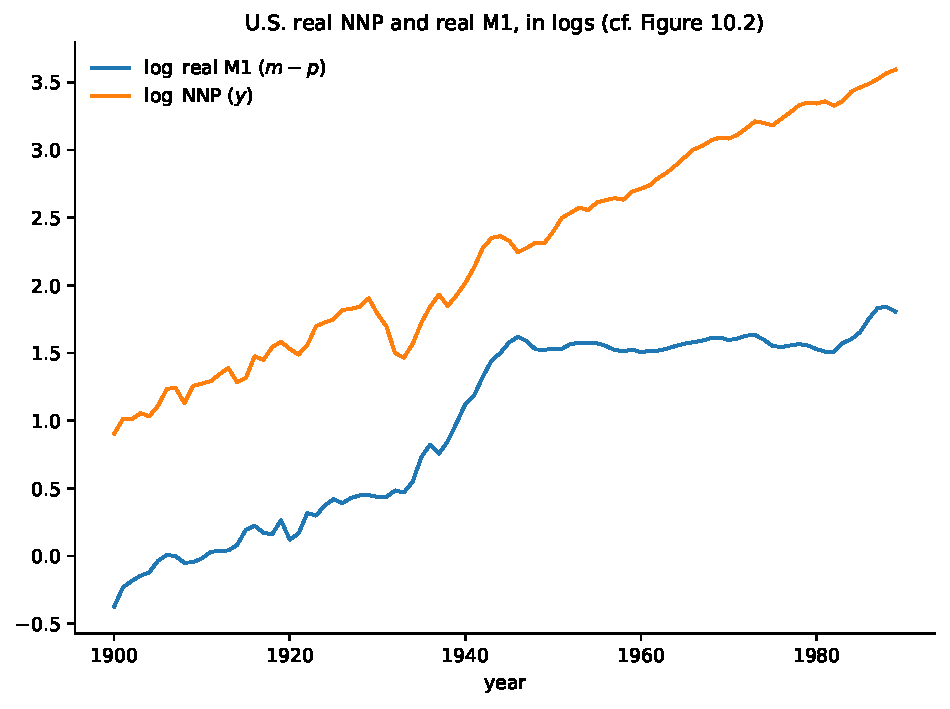
\includegraphics[width=0.82\textwidth]{figures/ch10_money_levels.pdf}
\caption{Log real M1 $(m-p)$ and log NNP $(y)$, 1900--1989 (cf.\ the book's Figure 10.2).}
\label{fig:ch10levels}
\end{figure}

\begin{figure}[t]
\centering
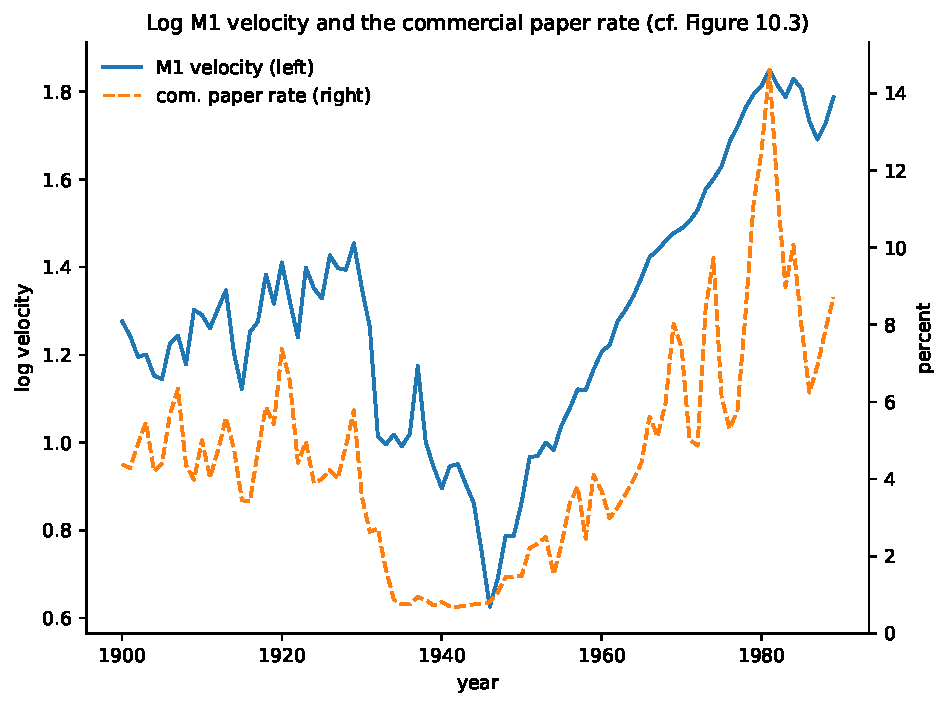
\includegraphics[width=0.82\textwidth]{figures/ch10_velocity.pdf}
\caption{Log M1 velocity $y-(m-p)$ (left scale) and the commercial paper rate $R$ (right scale) (cf.\
Figure 10.3).  Velocity tracks the interest rate, which is what suggests cointegration with a coefficient on
$y$ near unity.}
\label{fig:ch10velocity}
\end{figure}

(b) \emph{Engle--Granger test.}  The static (SOLS) regression of $m_t-p_t$ on a constant, $y_t$ and $R_t$
has residuals whose augmented autoregression without constant or time \bk{(10.3.2)} is estimated with $p=1$
lagged change --- also what BIC selects on the residuals.  The ADF $t$-statistic on $\hat z_{t-1}$ is
$-4.67$ when the cointegrating regression uses the full sample 1900--1989 (the book's ``about $-4.7$'') and
$-4.44$ when it uses 1903--1987, the DOLS sample of part (c).  Since the regressors $y$ and $R$ contain
drift/trend, case 2 of Section 10.3 applies with $g=2$ regressors, and the 5 percent asymptotic critical
value from \bk{Table 10.1(b)} is $-3.80$.  Either way the null of no cointegration is rejected (even the
2.5 percent value $-4.07$ is exceeded): the presumption that $m-p$ is cointegrated with $(y,R)$ survives
the test.

\begin{figure}[t]
\centering
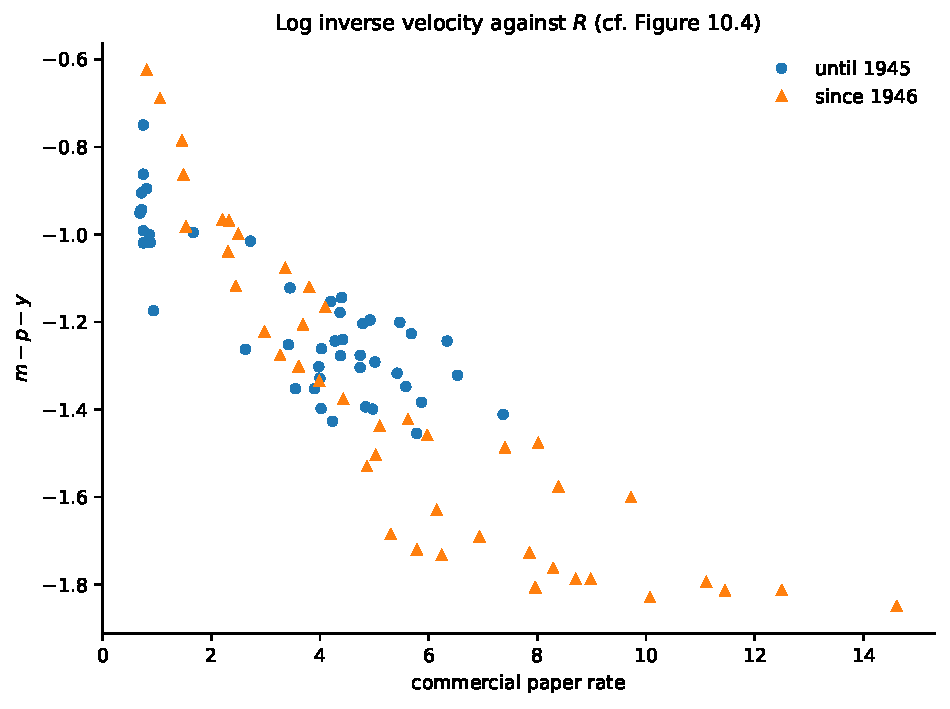
\includegraphics[width=0.82\textwidth]{figures/ch10_lucas.pdf}
\caption{Lucas's (1988) scatter: log inverse velocity $m-p-y$ against $R$, pre-1946 (circles) and postwar
(triangles) (cf.\ Figure 10.4).  Postwar points lie on the prewar relation.}
\label{fig:ch10lucas}
\end{figure}

(c) \emph{SOLS and DOLS, 1903--1987.}  The SOLS regression is the static regression of (b); the DOLS
regression adds $\Delta y_t$, $\Delta R_t$ and two leads and lags of each \bk{(10.5.2)}, which dictates the
sample period $t=1903,\dots,1987$ (85 observations, 13 regressors).  The long-run variance of the error is
estimated by fitting an AR(2) to the DOLS residuals over $t=1905,\dots,1987$ (83 observations), giving
\bk{(10.5.3)},
\[
\hat v_t=0.93806\,\hat v_{t-1}-0.13341\,\hat v_{t-2}+\hat e_t,\qquad \SSR=0.19843,
\]
and then \bk{(10.4.17)} with $\hat\sigma_e^2=\SSR/(T-p-K)=0.19843/(83-2-13)=0.0029181$:
\[
\hat\lambda_v^2=\frac{0.0029181}{(1-0.93806+0.13341)^2}=0.07647,
\qquad \hat\lambda_v\approx0.277,
\]
so the rescaling factor in \bk{(10.4.15)} is $\hat\lambda_v/s\approx0.277/0.096\approx2.9$.  Every figure
in \bk{Table 10.2} is reproduced:

\begin{center}
\begin{tabular}{lcccc}
\toprule
& $\gamma_y$ & $\gamma_R$ & $R^2$ & std.\ error of regression\\
\midrule
SOLS & $0.943$ & $-0.082$ & $0.959$ & $0.135$\\
DOLS & $0.970$ & $-0.101$ & $0.982$ & $0.096$\\
(rescaled std.\ errors) & $(0.046)$ & $(0.013)$\\
\bottomrule
\end{tabular}
\end{center}

With the rescaled standard errors, the $t$-statistic for a unitary income elasticity is
$(0.970-1)/0.046\approx-0.7$: the income elasticity is not significantly different from one, and the
interest semielasticity of about $-0.10$ (a one-percentage-point rise in $R$ lowers real money demand by
about 10 percent) is highly significant.

(d) \emph{Chow test at 1946.}  The augmented cointegrating regression of the question adds to \bk{(10.5.2)}
the three break variables $D_t$, $y_tD_t$, $R_tD_t$ with $D_t=\indic{t\ge1946}$.  The DOLS point estimates
reproduce \bk{Table 10.4}:
\[
\hat\gamma_y=0.925,\quad \hat\gamma_R=-0.090,\quad
\hat\delta_0=1.36,\quad \hat\delta_y=-0.52,\quad \hat\delta_R=0.048 .
\]
The AR(2) fit to the residuals of this 16-regressor regression gives
$\hat\sigma_e^2=\SSR/(83-2-16)$, $\hat\lambda_v=0.204$, and a rescaling factor
$\hat\lambda_v/s=0.204/0.0767=2.65$; the rescaled standard errors are $(0.142)$, $(0.026)$, $(0.72)$,
$(0.31)$, $(0.034)$, matching the table.

For the null $\delta_0=\delta_y=\delta_R=0$, the unscaled Wald statistic from the unrestricted regression is
$W_0=43.2$; rescaled by $(s/\hat\lambda_v)^2$ as prescribed in the text it is $W=6.13$, with a $\chi^2(3)$
p-value of $0.11$; divided by the number of restrictions ($F$-style) it is $2.04$ against the book's $1.85$
(p-value $0.60$).  The discrepancy appears to be in the precise scaling convention (degrees-of-freedom
corrections in $\hat\sigma_e^2$, whether $\hat\lambda_v$ is computed from the restricted or unrestricted
residuals, division by the number of restrictions): every variant tried in \texttt{code/ch10.py} gives a
statistic between $1.1$ and $6.4$, and every variant is insignificant at conventional levels.  The
conclusion is therefore the book's: the null of no structural change is not rejected, and the data are
consistent with Lucas's (1988) claim of a stable twentieth-century money demand --- the apparently different
postwar estimates of \bk{Table 10.3} ($\hat\gamma_y=0.269$, $\hat\gamma_R=-0.027$ for 1946--1987, against
$0.887$ and $-0.104$ for 1903--1945) reflect the near-collinearity of $y$ and $R$ in the postwar subsample
rather than a genuine shift, as Figure~\ref{fig:ch10lucas} makes visually plain.
\rmk{A caveat the book itself flags (footnote 16): the whole inference takes the cointegration rank $h=1$ as
given, although it was itself established by the pretest of part (b); the distribution of the DOLS estimates
does not account for the pretest uncertainty.}
\end{hee}

\end{document}
